\documentclass[11pt,a4paper]{article}
\usepackage[T1]{fontenc}
\usepackage[utf8]{inputenc}
\usepackage{lmodern,microtype,amsmath,amssymb,amsthm,mathtools,mathrsfs}
\usepackage[margin=24mm,headheight=15pt]{geometry}
\usepackage{booktabs,array,longtable,enumitem,xcolor,tikz,pgfplots,listings,fancyhdr,xurl}
\pgfplotsset{compat=1.18}
\usetikzlibrary{arrows.meta,calc,positioning}
\definecolor{navy}{HTML}{17324D}
\definecolor{teal}{HTML}{087F8C}
\definecolor{gold}{HTML}{B97520}
\definecolor{paperblue}{HTML}{EEF5F8}
\definecolor{inkgray}{HTML}{536171}
\usepackage[unicode,colorlinks=true,linkcolor=navy,citecolor=teal,urlcolor=teal,bookmarksnumbered=true]{hyperref}
\hypersetup{pdftitle={Prime Reciprocal Circles and the Riemann Zeta Function: A Unified Energy, Operator, and Sign Theory},pdfauthor={Research synthesis prepared for Keio},pdfsubject={Integrated mathematical working manuscript with additional proved synthesis results; no proof of the Riemann hypothesis is claimed}}
\pagestyle{fancy}\fancyhf{}
\fancyhead[L]{\small\color{inkgray}Prime circles and the Riemann zeta function}
\fancyhead[R]{\small\color{inkgray}Unified research manuscript}
\fancyfoot[C]{\small\thepage}
\renewcommand{\headrulewidth}{.3pt}
\setlength{\parskip}{3.5pt}\setlength{\parindent}{1.15em}
\setlength{\emergencystretch}{3em}
\setcounter{tocdepth}{1}
\makeatletter
\renewcommand*\l@section{\@dottedtocline{1}{1.5em}{3.2em}}
\renewcommand*\@pnumwidth{2.2em}
\makeatother
\numberwithin{equation}{section}
\allowdisplaybreaks[2]
\newtheorem{theorem}{Theorem}[section]
\newtheorem{proposition}[theorem]{Proposition}
\newtheorem{lemma}[theorem]{Lemma}
\newtheorem{corollary}[theorem]{Corollary}
\theoremstyle{definition}\newtheorem{definition}[theorem]{Definition}
\theoremstyle{remark}\newtheorem{remark}[theorem]{Remark}
\newcommand{\RH}{\mathrm{RH}}
\newcommand{\dd}{\,\mathrm{d}}
\newcommand{\ii}{\mathrm{i}}
\newcommand{\Reals}{\mathbb R}\newcommand{\Complex}{\mathbb C}\newcommand{\Disk}{\mathbb D}
\newcommand{\BP}{B_{\mathbb P}}
\DeclareMathOperator{\Li}{Li}
\DeclareMathOperator{\RePart}{Re}\DeclareMathOperator{\ImPart}{Im}
\newcommand{\norm}[1]{\left\lVert#1\right\rVert}
\newcommand{\abs}[1]{\left|#1\right|}
\newcommand{\eqdef}{\mathrel{:=}}
\newcommand{\source}[1]{\textcolor{inkgray}{#1}}
\newcommand{\Target}{\mathsf B}\newcommand{\one}{\mathbf1}
\newcommand{\C}{\mathbb C}\newcommand{\R}{\mathbb R}\newcommand{\D}{\mathbb D}
\newcommand{\T}{\mathbb T}\newcommand{\PP}{\mathbb P}\newcommand{\LP}{\mathcal{LP}}
\newcommand{\method}[2]{\subsection*{#1\quad #2}\addcontentsline{toc}{subsection}{#1\quad #2}}
\lstset{language=Python,basicstyle=\ttfamily\scriptsize,keywordstyle=\color{navy}\bfseries,commentstyle=\color{inkgray},stringstyle=\color{teal},breaklines=true,columns=fullflexible,keepspaces=true,showstringspaces=false,frame=single,rulecolor=\color{black!15},xleftmargin=2mm,xrightmargin=2mm,aboveskip=8pt,belowskip=8pt}
\begin{document}
\hypersetup{pageanchor=false}
\begin{titlepage}
\centering\vspace*{12mm}
{\large\color{teal}INTEGRATED MATHEMATICAL RESEARCH\par}
\vspace{11mm}
{\Huge\bfseries\color{navy}Prime Reciprocal Circles\par}
\vspace{4mm}
{\Huge\bfseries\color{navy}and the Riemann\par}
\vspace{3mm}
{\Huge\bfseries\color{navy}Zeta Function\par}
\vspace{9mm}
{\Large A Unified Energy, Operator, and Sign Theory\par}
\vspace{8mm}
{\large Research synthesis prepared for Keio\par}
{9 November 2026\par}
\vspace{10mm}
\begin{minipage}{.91\textwidth}
\textbf{Abstract.}
This manuscript reorganizes the reciprocal-prime-circle investigation into one theory of geometric deficits, centered prime-counting variance, critical Sobolev energy, Mellin singularities, and one-sided scalar sampling. Eleven earlier working notes are consolidated, including the seventh revision of the sign-sparsity analysis; the separate Mittag--Leffler project is excluded.

The synthesis also yields additional deductions. In the divergent regime, the circle deficit is asymptotic to $4\pi^2$ times the centered prime variance. Fixed harmonic deficits have an exact limiting ratio, giving a strict-gap criterion for RH. The previously known total Toeplitz leakage is localized in a single transverse eigenmode, with an explicit finite error estimate. Dilation differences become invertible co-analytic Toeplitz filters under the Laguerre transform, removing the unknown centering constant without removing the zero obstruction. Nonlinear positive-part moments have an exact growth spectrum; all critically damped $L^r$ endpoints with $r>1$ are finite. When $\Theta>1/2$, a renormalized limit at $r=1$ detects whether the supremal zero line is attained. Growing-threshold counts give a quantitative hierarchy of equivalent strip tests.

The proofs retain their quantifiers and distinguish unconditional implications, RH-conditional asymptotics, finite certificates, and an explicitly separated external fixed-strip input. No uniform bound for the original deficit, proof of RH, or historical-priority claim is made.
\end{minipage}
\vfill
\fcolorbox{navy!20}{paperblue}{\begin{minipage}{.88\textwidth}\centering
\textbf{One unchanged arithmetic target}\\[2mm]
$\displaystyle \RH\ \Longleftrightarrow\ \sup_ND_N<\infty
\ \Longleftrightarrow\ \int_2^\infty\mathcal A(x)_+\frac{dx}{x}<\infty.$\\[2mm]
\small The equivalences and auxiliary theorems are proved below. The finiteness assertion itself remains unproved.
\end{minipage}}
\vspace{5mm}
\end{titlepage}
\hypersetup{pageanchor=true}\pagenumbering{roman}
\begingroup\small\setlength{\parskip}{0pt}\tableofcontents\endgroup
\clearpage\pagenumbering{arabic}

\section{The synthesis: one object viewed through several structures}
\label{syn:introduction}

The research began with drawing prime-indexed arcs and asking whether the resulting geometry could test primality or constrain zeta zeros. The first proposal, an arc of angle $p\pi$, is degenerate modulo $2\pi$: every odd prime gives a half-turn. Replacing it by a $1/p$-turn arc is a change of construction, not an equivalent transformation. All subsequent arithmetic in this manuscript concerns the reciprocal construction.

The resulting sequence is informative only after its deterministic drift has been accounted for. Write
\begin{align}
S(x)&=\sum_{p\le x}p^{-1},&
E(x)&=S(x)-\log\log x-B_{\mathbb P},\label{syn:defs1}\\
P(x)&=\pi(x)-\Li_2(x),&
\Li_2(x)&=\int_2^x\frac{dt}{\log t},\label{syn:defs2}\\
\mathcal A(X)&=\int_2^X P(x)x^{-3/2}\,dx,&
\Theta&=\sup_{\zeta(\rho)=0,\ 0<\Re\rho<1}\Re\rho,
\quad\delta=\Theta-\tfrac12.\label{syn:defs3}
\end{align}
Here $B_{\mathbb P}$ is the prime Mertens constant. Prime-endpoint geometry uses
\begin{gather}
U_n=\exp\{2\pi i(S(p_n)-\log\log p_n)\},\quad
w_n=p_{n+1}-p_{n-1},\quad W_N=\sum_{n=2}^Nw_n,\label{syn:defs4}\\
D_N^{(m)}=W_N-\left|\sum_{n=2}^Nw_nU_n^m\right|,
\qquad D_N=D_N^{(1)}.\label{syn:defs5}
\end{gather}
The finite statistic $D_N$ requires neither $B_{\mathbb P}$ nor a zero of $\zeta$. Its relation to those analytic objects is a theorem, not a property assumed in its definition.
For $r>0$ we also write $\mathscr M_r(X)=\int_2^X\mathcal A(x)_+^r\,dx/x$,
where $y_+=\max(y,0)$.

\subsection{What the combination adds}

The added results are assembled from different mechanisms, rather than from renaming a target. Table~\ref{syn:table:new} separates their mathematical inputs from their precise output. The underlying tools---Taylor expansion, least squares, min--max theory, Laplace transforms, and almost periodicity---are classical. ``Added'' means derived and written out in this consolidation; it does not assert that no equivalent result exists in the literature.

\begin{longtable}{@{}p{.22\textwidth}p{.33\textwidth}p{.39\textwidth}@{}}
\caption{Additional synthesis results and their proof mechanisms.}\label{syn:table:new}\\
\toprule
Result & Structures combined & Exact conclusion\\\midrule\endfirsthead
\toprule Result & Structures combined & Exact conclusion\\\midrule\endhead
Sharp geometric comparison & Tangent covariance, prime-gap quadrature, and zero-forced lower growth & If RH fails, $D_N\sim4\pi^2V(p_{N+1})$, where $V(X)=\min_c\int_2^X(E-c)^2$.\\[3pt]
Harmonic ratio dichotomy & Concentration on a circle and the finite-energy criterion & For any fixed integer $m\ge2$, $\lim D_N^{(m)}/D_N<m^2$ exactly when RH holds; otherwise the limit is $m^2$.\\[3pt]
Single-mode spectral collapse & The tangent expansion of a moment curve and a finite Schur complement estimate & If $D_N\to\infty$, the second eigenvalue of the $(m+1)$-dimensional Toeplitz Gram matrix is asymptotic to $\binom{m+2}{3}D_N$; all later eigenvalues are $o(D_N)$.\\[3pt]
Constant-free Hardy coordinates & Multiplicative dilation, Laguerre functions, and a singular inner multiplier & On $L^2$, a dilation difference is represented by $I-qM_{\Theta_{L,\alpha}}^*$, with bounded inverse and sharp norm bounds; its zero-induced Taylor radius is unchanged.\\[3pt]
Nonlinear critical spectrum & Positive-part sampling, growth exponents, and weighted $L^r$ estimates & $\limsup\log(1+\mathscr M_r(X))/\log X=r\delta$, and $\int_2^\infty\mathcal A_+^r x^{-r\delta-1}dx<\infty$ for every $r>1$.\\[3pt]
Edge residue and count thresholds & Rectified almost-periodic zero profiles and positive series & When $\delta>0$, a normalized $r\downarrow1$ limit detects an attained supremal line; counts above $n^\lambda$ have a sharp transition at $\lambda=k\delta$.\\
\bottomrule
\end{longtable}

The strict harmonic criterion deserves care. Every finite ratio is already strictly below $m^2$ once at least two distinct phases are present. The unresolved issue is whether a positive gap survives the limit. Likewise, critical $L^r$ finiteness for $r>1$ is a proved endpoint result, but its damping depends on the actual zero supremum and it supplies no new numerical bound for $\Theta$.

\subsection{The common arithmetic obstruction}

Several apparently different targets reduce to the same finiteness statement. With the definitions and endpoint conventions proved later,
\begin{align}
\RH
&\Longleftrightarrow E\in L^2(2,\infty)
\Longleftrightarrow \sup_ND_N<\infty
\Longleftrightarrow \sup_XV(X)<\infty\notag\\
&\Longleftrightarrow \sup_X\{R_4(X)+\tfrac34\log\log X\}<\infty
\Longleftrightarrow \mu\in H^{-1}_{1/2}(\mathbb R)\notag\\
&\Longleftrightarrow \mathcal A(X)\le0\ \hbox{eventually}
\Longleftrightarrow\int_2^\infty\mathcal A(x)_+\frac{dx}{x}<\infty.
\label{syn:masterchain}
\end{align}
The measure $\mu$ is the critically weighted prime measure minus its continuous main term. The correlation $R_4$ is defined by a finite-cutoff kernel; there is no divergent infinite double sum hidden in the notation. These objects and every arrow in \eqref{syn:masterchain} receive proofs below. In particular, a Fourier transform of $\mu$ is used only after the required distributional or Sobolev membership is established.

\begin{figure}[htbp]\centering
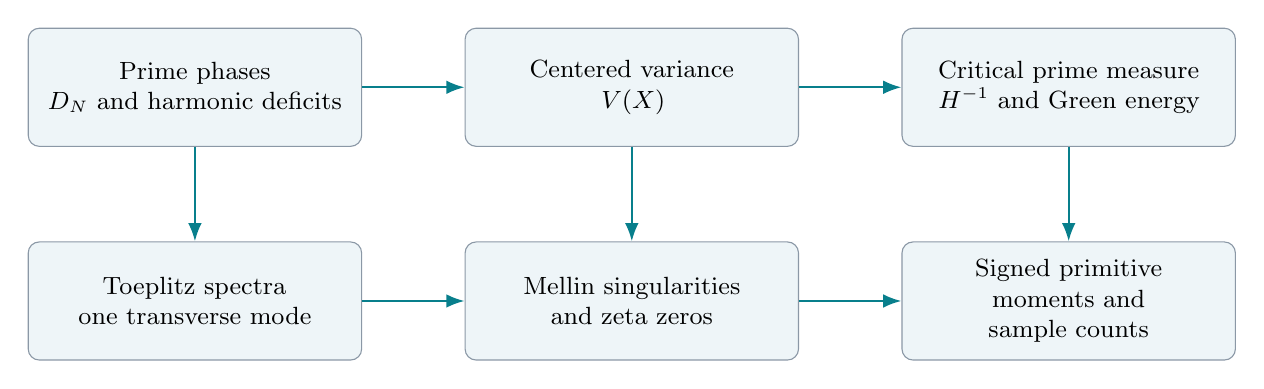
\begin{tikzpicture}[node distance=12mm and 13mm,>=Latex,
box/.style={draw=navy!50,rounded corners,fill=paperblue,align=center,text width=40mm,minimum height=15mm,font=\small},
arr/.style={->,thick,teal}]
\node[box] (circle) {Prime phases\\$D_N$ and harmonic deficits};
\node[box,right=of circle] (var) {Centered variance\\$V(X)$};
\node[box,right=of var] (measure) {Critical prime measure\\$H^{-1}$ and Green energy};
\node[box,below=of circle] (toeplitz) {Toeplitz spectra\\one transverse mode};
\node[box,below=of var] (zero) {Mellin singularities\\and zeta zeros};
\node[box,below=of measure] (scalar) {Signed primitive\\moments and sample counts};
\draw[arr] (circle)--(var);\draw[arr] (var)--(measure);
\draw[arr] (circle)--(toeplitz);\draw[arr] (var)--(zero);
\draw[arr] (measure)--(scalar);\draw[arr] (zero)--(scalar);
\draw[arr] (toeplitz)--(zero);
\end{tikzpicture}
\caption{The organization of the synthesis. Arrows denote proved transfers developed in the text, not independent proofs of finite energy. The additional results quantify several of these transfers.}
\end{figure}

\subsection{Status, assumptions, and the meaning of progress}

An equivalence is a proved theorem even when both equivalent assertions remain undecided. It does not by itself narrow the set of possible zeta zeros. The concrete progress here consists of exact constants, error controls, spectral localization, removal of finite-cutoff artifacts, and identification of which quantifiers still require an arithmetic estimate.

The main synthesis results do not use a fixed zero-free strip to the left of $1$. Some earlier degree-four arguments did import a stated 2026 preprint result. In this consolidated manuscript those applications are read under the explicit hypothesis
\begin{equation}
(H_b):\qquad \Theta\le b<7/8,
\label{syn:fixedstrip}
\end{equation}
or under the directly stated finite eighth-moment hypothesis. The preprint statements and consequences are documented in the polynomial module; their full proofs and formalization are not independently rebuilt here. No such external claim is silently promoted to a result of this manuscript. Purely finite linear algebra and the abstract extremal-polynomial theorems retain their stated hypotheses and do not require $(H_b)$.

Standard inputs are cited where used: Mertens' theorem and the prime number theorem; Euler products and the functional equation; conditional mean-square estimates for the prime-counting error; Stechkin--Popov lower mean estimates; prime-gap estimates; and the stated sieve and large-value theorems. The RH-conditional mean-square estimate is materially stronger for this purpose than merely inserting a pointwise RH bound. The historical studies of integrated prime errors provide relevant context, not a claim of priority for the equivalent formulations recorded here.

\subsection{Editorial scope and reproducibility}

The eleven source notes are listed in the provenance section. Their common notation and title matter have been consolidated, duplicated foundations are referred to the first proof where possible, and independent proof routes are retained when their different hypotheses matter. The eighty-method transfer ledger is retained as an audit of applicability, not a claim that eighty unrelated theorems have proved RH. The theta-kernel and finite-field analyses are included because they arose in the zeta investigation, even though those auxiliary results have their own scope.

Earlier finite numerical certificates remain explicitly finite. New computations check the synthesis constants on finite model sequences and the algebraic identities on actual primes; they do not test any universal RH assertion. All text, diagrams, tables, and displayed reproduction code needed for this version are contained in this single \TeX{} file. The separate Poisson-coupling manuscript for Mittag--Leffler laws is not included.

\clearpage


\clearpage
\part{Foundations: reciprocal primes and geometric energy}\label{part:foundation}


% Consolidated source: Prime_Reciprocal_Circles.tex, section-index 0
\section{The construction and the scope of the claims}\label{pc:sec:foundation}

All logarithms are natural. The letter \(p\) always denotes a prime,
and \(p_n\) is the \(n\)-th prime, with \(p_1=2\). Define
\begin{equation}\label{pc:eq:basic}
 S(x)=\sum_{p\le x}\frac1p,\qquad
 E(x)=S(x)-\log\log x-\BP,\qquad x\ge2,
\end{equation}
where the exact Meissel--Mertens constant is
\begin{equation}\label{pc:eq:mertensconstant}
 \BP=\gamma+\sum_p\left(\log(1-p^{-1})+p^{-1}\right)
 =0.26149721284764278375542683860869585905\ldots .
\end{equation}
The series in \eqref{pc:eq:mertensconstant} converges absolutely.
Mertens' theorem gives \(E(x)=O(1/\log x)\); in particular \(E\) is
bounded and tends to zero. We use the notation of
\eqref{pc:eq:basic} consistently, rather than the several different
constants sometimes denoted \(B_1\) in the literature
\cite{pc:zhao,pc:mertens}.

Let \(\mathcal Z\) be the multiset of nontrivial zeros of \(\zeta\), and set
\begin{equation}\label{pc:eq:theta}
 \Theta=\sup_{\rho\in\mathcal Z}\Re\rho.
\end{equation}
The functional equation and the location of the zeros give
\(1/2\le\Theta\le1\), and RH is equivalent to \(\Theta=1/2\).
We do not assume that the supremum is attained.

\subsection{What a complete turn actually means}

The reciprocal construction adds \(1/p\) of a turn at each prime:
\[
 C(x)=e^{2\pi\ii S(x)}.
\]
The lifted number of turns is the real number \(S(x)\), not just the
point \(C(x)\). The number of completed turns is \(\lfloor S(x)\rfloor\).
Every finite \(S(x)\) is an exactly computable rational number.

\begin{proposition}[No exact closure at a prime endpoint]\label{pc:prop:noexact}
For every nonempty finite set of distinct primes, the sum of their
reciprocals is not an integer. Consequently \(C(p_n)\ne1\) for every
\(n\ge1\).
\end{proposition}
\begin{proof}
Let \(Q\) be the product of the primes in the set and let
\(A=\sum_{p\mid Q}Q/p\). For each \(q\mid Q\),
\(A\equiv Q/q\not\equiv0\pmod q\). Thus \(\gcd(A,Q)=1\), and
the reduced denominator of \(A/Q\) is \(Q>1\).
\end{proof}

If \(q_m\) is the first prime with \(S(q_m)>m\), then
\begin{equation}\label{pc:eq:overshoot}
 0<S(q_m)-m<\frac1{q_m}.
\end{equation}
A continuously drawn arc passes the integer turn during the final
step; its endpoint overshoots it. The fact that \(q_m\) is prime is
built into this indexing and is not a primality test.

The smooth prediction for the \(m\)-th crossing is
\[
 X_m=\exp\!\bigl(\exp(m-\BP)\bigr).
\]
If one formally replaces the local error by
\(E(x)\approx1/(\sqrt{x}\log x)\), then a first-order inversion gives
\(X_m-q_m\approx\sqrt{X_m}\). This explains why a square-root scale is
natural. It does not establish an exact displacement or a uniform
one-sided law. Zeta zeros contribute oscillations, and the final
prime step is discrete. The theorems below concern the entire error
function, not just the sparse sequence of turn crossings.

\subsection{The exact centered circle}

Introduce the reference motion and the relative phase
\begin{equation}\label{pc:eq:circle}
 C_0(x)=e^{2\pi\ii(\log\log x+\BP)},\qquad
 Z(x)=C(x)\overline{C_0(x)}=e^{2\pi\ii E(x)}.
\end{equation}
Their chord distance satisfies the exact identity
\begin{equation}\label{pc:eq:chord}
 |C(x)-C_0(x)|^2=|Z(x)-1|^2=4\sin^2(\pi E(x)).
\end{equation}
Because \(E(x)\to0\), this is asymptotic to \(4\pi^2 E(x)^2\).
The principal argument is not a globally valid replacement for the
lift \(E\): for example \(E(2)\approx0.6050>1/2\). Only its eventual
smallness is needed for the energy comparisons.

\begin{figure}[htbp]
\centering
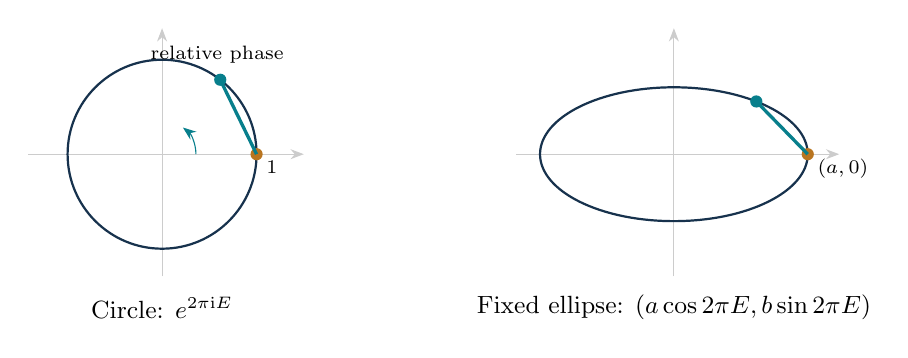
\begin{tikzpicture}[scale=1,>=Stealth]
 \begin{scope}[xshift=-3.4cm]
  \draw[black!20,->](-1.7,0)--(1.8,0);
  \draw[black!20,->](0,-1.55)--(0,1.6);
  \draw[navy,thick](0,0) circle(1.2);
  \fill[gold](1.2,0) circle(2.2pt);
  \fill[teal]({1.2*cos(52)},{1.2*sin(52)}) circle(2.2pt);
  \draw[teal,very thick](1.2,0)--({1.2*cos(52)},{1.2*sin(52)});
  \draw[->,teal](0.43,0) arc(0:52:0.43);
  \node at(0,-1.95){\small Circle: \(e^{2\pi\ii E}\)};
  \node[right] at(1.2,-0.16){\scriptsize \(1\)};
  \node[above] at(0.7,1.03){\scriptsize relative phase};
 \end{scope}
 \begin{scope}[xshift=3.1cm]
  \draw[black!20,->](-2,0)--(2.1,0);
  \draw[black!20,->](0,-1.55)--(0,1.6);
  \draw[navy,thick](0,0) ellipse(1.7 and .85);
  \fill[gold](1.7,0) circle(2.2pt);
  \fill[teal]({1.7*cos(52)},{.85*sin(52)}) circle(2.2pt);
  \draw[teal,very thick](1.7,0)--({1.7*cos(52)},{.85*sin(52)});
  \node at(0,-1.95){\small Fixed ellipse: \((a\cos2\pi E,b\sin2\pi E)\)};
  \node[right] at(1.7,-0.18){\scriptsize \((a,0)\)};
 \end{scope}
\end{tikzpicture}
\caption{The same phase on a circle and a fixed nondegenerate ellipse.
The squared chord distances have comparable tail integrals when
\(a,b>0\). The illustration is schematic, not a plot of prime data.}
\end{figure}

\subsection{Established inputs and deductions in this note}

The analytic inputs are Mertens' theorem, the Euler product and
functional equation, the conditional mean-square estimate stated in
Section~\ref{pc:sec:energy}, and the estimate
\begin{equation}\label{pc:eq:grosswald}
 \pi(x)-\operatorname{li}(x)=O_\Theta\!\left(\frac{x^\Theta}{\log x}\right),
 \qquad \frac12<\Theta<1.
\end{equation}
The last estimate is due to Grosswald; the precise form we use is
recorded in Zhao's equation~(24) \cite{pc:grosswald,pc:zhao}.
These are cited inputs, not results first proved here.
The Mellin converse, discrete comparisons, vector-deficit identities,
growth laws, and transform consequences are established below.
Their historical priority has not been investigated.


% Consolidated source: Prime_Reciprocal_Circles.tex, section-index 1
\section{Prime zeta decomposition and the Mellin obstruction}\label{pc:sec:mellin}

For \(\Re s>1\), the prime zeta function is
\(P(s)=\sum_p p^{-s}\). Stieltjes integration gives
\begin{equation}\label{pc:eq:primezeta}
 P(s)=\int_{2^-}^{\infty}x^{1-s}\dd S(x)
     =(s-1)\int_2^\infty S(x)x^{-s}\dd x.
\end{equation}
The Euler product, followed by absolutely convergent summation, gives
\begin{equation}\label{pc:eq:euler}
 \log\zeta(s)=\sum_{k\ge1}\frac{P(ks)}k,\qquad
 P(s)=\sum_{k\ge1}\frac{\mu(k)}k\log\zeta(ks).
\end{equation}
The logarithms in this half-plane use the Euler-product branch
\cite{pc:dlmf-zeta,pc:froberg}. Each summand
\(p^{-s}=p^{-\Re s}e^{-\ii(\Im s)\log p}\) is a rotating vector,
but this observation alone does not continue the prime series to the
critical line. The continuation must be justified analytically.

Put
\[
 F(s)=\int_2^\infty E(x)x^{-s}\dd x,\qquad
 c=\log\log2+\BP .
\]
Initially \(\Re s>1\). Integrating the elementary part of \(S\) in
\eqref{pc:eq:primezeta} gives
\begin{equation}\label{pc:eq:PF}
 P(s)=(s-1)F(s)+c\,2^{1-s}
      +\int_2^\infty\frac{x^{-s}}{\log x}\dd x.
\end{equation}
Consequently
\begin{equation}\label{pc:eq:Pprime}
 P'(s)=F(s)+(s-1)F'(s)
       -c(\log2)2^{1-s}-\frac{2^{1-s}}{s-1}.
\end{equation}
Also,
\begin{equation}\label{pc:eq:logderivative}
 \frac{\zeta'(s)}{\zeta(s)}
 =P'(s)+\sum_{k\ge2}P'(ks).
\end{equation}
The sum on the right is holomorphic for \(\Re s>1/2\), since on
every compact sub-half-plane it is dominated by
\[
 \sum_p\frac{(\log p)p^{-2\sigma}}{1-p^{-\sigma}}<\infty,
 \qquad \sigma>1/2.
\]

\begin{lemma}[Zero exclusion from Mellin continuation]\label{pc:lem:mellin}
Suppose \(a\ge1/2\), and the germ \(F\) extends holomorphically to
\(\Re s>a\). Then \(\zeta(s)\) has no zeros in that half-plane.
\end{lemma}
\begin{proof}
Equations \eqref{pc:eq:Pprime} and \eqref{pc:eq:logderivative} provide a
meromorphic continuation of \(\zeta'/\zeta\) to this half-plane
whose only possible pole is the one at \(s=1\).
A zero of \(\zeta\) there would give an additional pole of its
logarithmic derivative, with positive integral residue.
The identity theorem for meromorphic functions rules this out.
\end{proof}

We shall also need the obstruction at \(s=1/2\).
Define the entire function
\[
 J_0(s)=c\,2^{1-s}-\gamma-\log\log2
       -\sum_{j\ge1}\frac{[-(s-1)\log2]^j}{j\,j!},
\]
and put \(R_0(s)=\sum_{k\ge2}P(ks)/k\), holomorphic for
\(\Re s>1/2\). The exponential-integral expansion in
\eqref{pc:eq:PF} gives
\begin{equation}\label{pc:eq:Fanalytic}
 F(s)=
 \frac{\log((s-1)\zeta(s))-R_0(s)-J_0(s)}{s-1}.
\end{equation}
The branch is obtained from real \(s>1\) on any simply connected
zero-free region. At \(s=1\), the numerator vanishes because
\(R_0(1)=\gamma-\BP\), \(J_0(1)=\BP-\gamma\), and
\((s-1)\zeta(s)\) takes the value \(1\).
Thus \(s=1\) is removable.

\begin{lemma}[Prime-square singularity]\label{pc:lem:square}
The germ \(F\) cannot extend holomorphically to a half-plane
\(\Re s>a\) with \(a<1/2\).
Along the real continuation from the right,
\begin{equation}\label{pc:eq:square}
 F(1/2+\varepsilon)=-\log\varepsilon+O(1),
 \qquad \varepsilon\downarrow0.
\end{equation}
\end{lemma}
\begin{proof}
The factor \((s-1)\zeta(s)\) has no zero on the real interval
\(1/2\le s\le1\); in particular \(\zeta(1/2)<0\).
The \(k=2\) term in \(R_0\) is
\[
 \tfrac12 P(1+2\varepsilon)
 =-\tfrac12\log(2\varepsilon)+O(1),
\]
whereas its \(k\ge3\) terms remain holomorphic near \(s=1/2\).
Equation \eqref{pc:eq:Fanalytic} therefore proves \eqref{pc:eq:square}.
Equivalently, if \(P'\) were regular there,
\eqref{pc:eq:logderivative} would give a residue \(-1/2\) from
\(P'(2s)\), which is impossible for a logarithmic derivative.
\end{proof}


% Consolidated source: Prime_Reciprocal_Circles.tex, section-index 2
\section{The exact quadratic energy criterion}\label{pc:sec:energy}

\begin{theorem}[Scalar, circle, and fixed-ellipse energies]\label{pc:thm:energy}
The following statements are equivalent:
\begin{enumerate}[label=(\roman*),itemsep=2pt]
 \item RH holds.
 \item \(\displaystyle\int_2^\infty E(x)^2\dd x<\infty\).
 \item \(\displaystyle\int_2^\infty|Z(x)-1|^2\dd x<\infty\).
 \item For any fixed \(a,b>0\),
 \[
 \int_2^\infty
 \left[(a\cos(2\pi E(x))-a)^2+b^2\sin^2(2\pi E(x))\right]\dd x<\infty .
 \]
\end{enumerate}
\end{theorem}

\begin{proof}
Assume (ii). Cauchy--Schwarz shows that \(F\) and all its derivatives
under the integral sign are holomorphic for \(\Re s>1/2\).
For example, on a compact sub-half-plane,
\[
 \int_2^\infty |E(x)|x^{-\sigma}(\log x)^j\dd x
 \le \norm{E}_2
 \left(\int_2^\infty x^{-2\sigma}(\log x)^{2j}\dd x\right)^{1/2}.
\]
Lemma~\ref{pc:lem:mellin} excludes zeros to the right of \(1/2\);
the functional equation excludes those to the left.
Hence (ii) implies RH.

For the forward direction we give the analytic argument, rather
than infer mean-square convergence from a pointwise RH estimate.
The established conditional estimate of Cramer's type is
\begin{equation}\label{pc:eq:cramer}
 \RH\quad\Longrightarrow\quad
 \int_X^{2X}(\psi(t)-t)^2\dd t\ll X^2.
\end{equation}
See Brent--Platt--Trudgian \cite{pc:bpt} for this mean-square framework.
Since \(\psi(x)-\vartheta(x)=O(\sqrt{x})\), the same upper bound
holds for \(R(x)=\vartheta(x)-x\).
Set \(f(x)=R(x)/(x\log x)\). On dyadic intervals,
\[
 \int_X^{2X}f(x)^2\dd x\ll\frac1{\log^2X}.
\]
Summing over \(X=2^j\) proves \(f\in L^2(2,\infty)\).
Partial summation, with the limiting constant in
\eqref{pc:eq:mertensconstant}, gives
\begin{equation}\label{pc:eq:hardyidentity}
 E(x)=f(x)-\int_x^\infty
       \frac{f(t)}t\left(1+\frac1{\log t}\right)\dd t .
\end{equation}
The adjoint Hardy operator
\(Hg(x)=\int_x^\infty g(t)t^{-1}\dd t\) satisfies
\(\norm{Hg}_2\le2\norm{g}_2\).
For compactly supported \(g\), integration by parts followed by
Cauchy--Schwarz proves this inequality; truncation proves the
general case. The multiplier in \eqref{pc:eq:hardyidentity} is bounded
for \(t\ge2\). Therefore \(E\in L^2\).
This also explains the forward assertion in Zhao's Lemma~9
\cite{pc:zhao}.

By \eqref{pc:eq:chord} and \(E(x)\to0\), the integrands in (ii) and
(iii) are comparable on a tail. Initial compact intervals are
irrelevant to finiteness. Finally, if
\(d_{a,b}(t)^2=a^2(\cos2\pi t-1)^2+b^2\sin^22\pi t\), then
\begin{equation}\label{pc:eq:ellipsebounds}
 \min(a^2,b^2)|e^{2\pi\ii t}-1|^2
 \le d_{a,b}(t)^2
 \le \max(a^2,b^2)|e^{2\pi\ii t}-1|^2.
\end{equation}
This proves (iii) if and only if (iv).
\end{proof}

\begin{remark}[Measure and tail rate]
The proof also gives, under RH,
\(\int_X^\infty E(x)^2\dd x\ll1/\log X\).
The measure \(\dd x\) matters: under \(x=e^t\), it becomes
\(e^t\dd t\). Replacing it by \(\dd t\) without the factor
would define a different criterion. Moreover, the common pointwise
RH bound \(E(x)=O(x^{-1/2}\log x)\) alone gives a divergent
majorant for \(\int E^2\); the mean-square input is essential.
\end{remark}


% Consolidated source: Prime_Reciprocal_Circles.tex, section-index 3
\section{The complete integrability spectrum and geometric losses}\label{pc:sec:spectrum}

Partial summation using \(\pi(x)-\operatorname{li}(x)\) gives the exact tail formula
\begin{equation}\label{pc:eq:pitail}
 E(x)=\frac{\pi(x)-\operatorname{li}(x)}x
       -\int_x^\infty\frac{\pi(t)-\operatorname{li}(t)}{t^2}\dd t .
\end{equation}
For \(1/2<\Theta<1\), \eqref{pc:eq:grosswald} implies
\begin{equation}\label{pc:eq:Etheta}
 E(x)=O_\Theta\!\left(\frac{x^{\Theta-1}}{\log x}\right).
\end{equation}

\begin{theorem}[All finite powers, including the endpoint]\label{pc:thm:Lq}
For every finite \(q>0\),
\begin{equation}\label{pc:eq:Lq}
 \int_2^\infty |E(x)|^q\dd x<\infty
 \quad\Longleftrightarrow\quad
 \Theta\le1-\frac1q.
\end{equation}
In particular no such integral converges for \(0<q<2\).
If \(\Theta<1\), the exact threshold is
\(q=1/(1-\Theta)\), and the threshold itself is included.
If \(\Theta=1\), no finite \(q\) works.
\end{theorem}
\begin{proof}
For \(q>1\), H\"older's inequality makes \(F\) holomorphic in
\(\Re s>1-1/q\) whenever \(E\in L^q\).
If \(q\ge2\), Lemma~\ref{pc:lem:mellin} gives the stated necessary
condition. If \(1<q<2\), this continuation crosses \(s=1/2\),
contradicting Lemma~\ref{pc:lem:square}.
For \(0<q\le1\), boundedness of \(E\) would imply
\(E\in L^r\) for any chosen \(1<r<2\), again a contradiction.

For sufficiency, when \(\Theta=1/2\), Theorem~\ref{pc:thm:energy}
and boundedness of \(E\) give \(E\in L^q\) for all \(q\ge2\).
When \(1/2<\Theta<1\), use \eqref{pc:eq:Etheta}.
At the limiting value \(q(1-\Theta)=1\), the majorant is
\(1/[x(\log x)^q]\), which is integrable because \(q>2\).
Larger \(q\) are easier.
\end{proof}

\begin{theorem}[Exact weighted quadratic threshold]\label{pc:thm:weighted}
For every real \(\eta\),
\begin{equation}\label{pc:eq:weighted}
 \int_2^\infty x^{1-2\eta}E(x)^2\dd x<\infty
 \quad\Longleftrightarrow\quad \eta\ge\Theta .
\end{equation}
\end{theorem}
\begin{proof}
Weighted Cauchy--Schwarz makes \(F\) holomorphic in
\(\Re s>\eta\). If \(\eta<1/2\), Lemma~\ref{pc:lem:square}
gives a contradiction; otherwise Lemma~\ref{pc:lem:mellin}
requires \(\eta\ge\Theta\).

For sufficiency at \(\eta=\Theta\), use
Theorem~\ref{pc:thm:energy} when \(\Theta=1/2\),
\eqref{pc:eq:Etheta} when \(1/2<\Theta<1\), and Mertens'
\(E(x)=O(1/\log x)\) when \(\Theta=1\).
The last two cases give the integrable majorant
\(1/[x(\log x)^2]\). For \(\eta>\Theta\) the weight is smaller.
\end{proof}

\begin{corollary}[Order of contact of a curve]\label{pc:cor:contact}
Suppose a continuous curve \(\Gamma:\mathbb R\to\mathbb R^d\) satisfies
\(\Gamma(t)-\Gamma(0)=v t^k+O(t^{k+1})\) as \(t\to0\),
where \(k\) is a positive integer and \(v\ne0\).
Then
\begin{equation}\label{pc:eq:contact}
 \int_2^\infty\norm{\Gamma(E(x))-\Gamma(0)}^2\dd x<\infty
 \quad\Longleftrightarrow\quad
 \Theta\le1-\frac1{2k}.
\end{equation}
\end{corollary}
\begin{proof}
On a tail the integrand is bounded above and below by positive
constants times \(|E(x)|^{2k}\). Apply Theorem~\ref{pc:thm:Lq}.
\end{proof}

A fixed nondegenerate ellipse has \(k=1\) and preserves the RH
criterion. Projecting onto its horizontal axis gives
\((a\cos2\pi E-a)^2\asymp E^4\), so the criterion becomes
\(\Theta\le3/4\). This is an exact classification, not merely a
failure of the original proof.

There is also a continuous transition between these cases.
For \(\lambda\ge0\), consider the moving ellipse point
\[
 \Gamma_\lambda(x)=
 \bigl(\cos(2\pi E(x)),\,x^{-\lambda}\sin(2\pi E(x))\bigr).
\]
Its distance from \((1,0)\) has tail square comparable to
\(E(x)^4+x^{-2\lambda}E(x)^2\). Theorems~\ref{pc:thm:Lq}
and \ref{pc:thm:weighted} therefore give
\begin{equation}\label{pc:eq:shrinkingellipse}
 \int_2^\infty\norm{\Gamma_\lambda(x)-(1,0)}^2\dd x<\infty
 \quad\Longleftrightarrow\quad
 \Theta\le\min\left(\frac34,\frac12+\lambda\right).
\end{equation}
Thus pointwise nondegeneracy is insufficient if an axis tends to zero.

\begin{table}[htbp]
\centering
\small
\begin{tabular}{@{}lll@{}}
\toprule
Observation & Tail sensitivity & Exact finite-energy condition\\
\midrule
Circle / fixed nondegenerate ellipse & \(E^2\) & \(\Theta=1/2\)\\
Horizontal projection & \(E^4\) & \(\Theta\le3/4\)\\
Curve with contact order \(k\) & \(E^{2k}\) &
 \(\Theta\le1-1/(2k)\)\\
Axis \(b(x)=x^{-\lambda}\) & \(E^4+x^{-2\lambda}E^2\) &
 \(\Theta\le\min(3/4,1/2+\lambda)\)\\
\bottomrule
\end{tabular}
\caption{How changing the geometry changes the zero-location condition.}
\end{table}


% Consolidated source: Prime_Reciprocal_Circles.tex, section-index 4
\section{Exact sampling at prime gaps and integers}\label{pc:sec:sampling}

Put
\[
 e_n=E(p_n),\qquad h_n=p_{n+1}-p_n,\qquad
 b_n=E(p_{n+1}^{-})=e_{n+1}-p_{n+1}^{-1}.
\]
On the interval \([p_n,p_{n+1})\) there is no prime jump, and
\[
 E(x)=e_n-\bigl(\log\log x-\log\log p_n\bigr).
\]

\begin{lemma}[A two-endpoint comparison]\label{pc:lem:gap}
For every \(n\ge1\),
\begin{equation}\label{pc:eq:gap}
 \frac{h_n}{24}(e_n^2+b_n^2)
 \le\int_{p_n}^{p_{n+1}}E(x)^2\dd x
 \le h_n(e_n^2+b_n^2).
\end{equation}
\end{lemma}
\begin{proof}
Write \(p=p_n,q=p_{n+1}\) and
\[
 y=\frac{\log\log x-\log\log p}{\log\log q-\log\log p}.
\]
Then \(E(x)=(1-y)e_n+yb_n\). The derivative \(\dd x/\dd y\)
has maximum-to-minimum ratio \(q\log q/(p\log p)<4\) by
Bertrand's postulate, while its integral is \(h_n\).
It is therefore between \(h_n/4\) and \(4h_n\).
Moreover,
\[
 \int_0^1((1-y)a+yb)^2\dd y
 =\frac{a^2+ab+b^2}{3}\ge\frac{a^2+b^2}{6}.
\]
This proves the lower bound. For the upper bound,
\(((1-y)a+yb)^2\le\max(a^2,b^2)\le a^2+b^2\)
throughout the interval.
\end{proof}

The jump correction has finite weighted square:
\begin{equation}\label{pc:eq:jumpcorrection}
 \sum_{n\ge1}\frac{h_n}{p_{n+1}^2}
 \le\sum_{n\ge1}\int_{p_n}^{p_{n+1}}\frac{\dd x}{x^2}
 =\frac12.
\end{equation}
Consequently replacing \(b_n\) by \(e_{n+1}\) preserves convergence.
For \(n\ge2\), set
\begin{equation}\label{pc:eq:weights}
 w_n=h_{n-1}+h_n=p_{n+1}-p_{n-1}.
\end{equation}

\begin{theorem}[The prime-endpoint criterion]\label{pc:thm:discrete}
One has
\begin{align}
 \RH
 &\Longleftrightarrow
 \sum_{n\ge2}w_nE(p_n)^2<\infty \label{pc:eq:discreteE}\\
 &\Longleftrightarrow
 \sum_{n\ge2}w_n|e^{2\pi\ii E(p_n)}-1|^2<\infty .
 \label{pc:eq:discretecircle}
\end{align}
If \(I(X)=\int_2^X E(x)^2\dd x\) and
\(A_N=\sum_{n=2}^N w_ne_n^2\), then
\begin{equation}\label{pc:eq:finitecomparison}
 I(p_N)\ll1+A_N\ll1+I(p_{N+1}).
\end{equation}
\end{theorem}
\begin{proof}
Sum \eqref{pc:eq:gap}. The elementary inequalities
\((a+b)^2\le2a^2+2b^2\) and
\(a^2\le2(a-b)^2+2b^2\), together with
\eqref{pc:eq:jumpcorrection}, give both the convergence statement
and \eqref{pc:eq:finitecomparison}. The finite initial endpoint
contributes only a constant. Theorem~\ref{pc:thm:energy}
and the tail equivalence \eqref{pc:eq:chord} finish the proof.
\end{proof}

The weight \(w_n\) records the amount of real \(x\)-space represented
by a prime endpoint. Dropping it changes the question. Sampling only
the primes at which an entire turn is crossed is much sparser and
is not covered by this theorem.

\begin{corollary}[Integer sampling]\label{pc:cor:integers}
\[
 \RH\quad\Longleftrightarrow\quad
 \sum_{m=2}^{\infty}E(m)^2<\infty
 \quad\Longleftrightarrow\quad
 \sum_{m=2}^{\infty}|Z(m)-1|^2<\infty.
\]
\end{corollary}
\begin{proof}
On \([m,m+1)\), \(S(x)=S(m)\) and
\[
 |E(x)-E(m)|\le\frac1{m\log m}.
\]
The difference between \(E\) and its integer-step sampling is in
\(L^2\). The result follows from Theorem~\ref{pc:thm:energy}.
\end{proof}


% Consolidated source: Prime_Reciprocal_Circles.tex, section-index 5
\section{A monotone geometric criterion without an input constant}\label{pc:sec:deficit}

Define, using no supplied value of \(\BP\),
\begin{equation}\label{pc:eq:U}
 U_n=\exp\left(2\pi\ii\left[S(p_n)-\log\log p_n\right]\right),
 \qquad n\ge2.
\end{equation}
Mertens' theorem implies \(U_n\to u_\infty=e^{2\pi\ii\BP}\).
With the weights in \eqref{pc:eq:weights}, put
\begin{align}
 W_N&=\sum_{n=2}^Nw_n=p_N+p_{N+1}-5, \label{pc:eq:W}\\
 M_N&=\sum_{n=2}^Nw_nU_n,\qquad m_N=M_N/W_N,\\
 D_N&=W_N-|M_N|,\qquad
 V_N=W_N-\frac{|M_N|^2}{W_N}. \label{pc:eq:DV}
\end{align}
Here \(D_N\) is the sum of the vector lengths minus the length of
their resultant. The quantity \(V_N\) is their weighted variance.

\begin{lemma}[Variance and vector deficit]\label{pc:lem:variance}
Let any unit vectors \(u_n\to u_\infty\) and positive weights
\(w_n\) satisfy \(W_N\to\infty\). Define \(M_N,m_N,D_N,V_N\)
as above and let
\(\mathcal J_N=\sum_{n=2}^Nw_n|u_n-u_\infty|^2\).
Then \(D_N,V_N\) are nonnegative and nondecreasing, and
\begin{align}
 V_N&=D_N(1+|M_N|/W_N), &D_N\le V_N\le2D_N, \label{pc:eq:variance1}\\
 V_N&=\sum_{n=2}^Nw_n|u_n-m_N|^2
      =\frac1{W_N}\sum_{2\le j<k\le N}w_jw_k|u_j-u_k|^2,
       \label{pc:eq:variance2}\\
 \mathcal J_N&=V_N+W_N|m_N-u_\infty|^2. \label{pc:eq:fixedcenter}
\end{align}
Moreover,
\begin{equation}\label{pc:eq:deficitequivalence}
 \sup_ND_N<\infty
 \ \Longleftrightarrow\
 \sup_NV_N<\infty
 \ \Longleftrightarrow\
 \mathcal J_\infty<\infty.
\end{equation}
When these quantities are finite,
\begin{equation}\label{pc:eq:deficitlimit}
 2D_\infty=V_\infty=\mathcal J_\infty.
\end{equation}
\end{lemma}
\begin{proof}
Expanding squares proves
\eqref{pc:eq:variance1}--\eqref{pc:eq:fixedcenter}.
The triangle inequality gives monotonicity of \(D_N\).
If a unit point \(u\) of weight \(w\) is appended to old quantities
\(W,m,V\), direct expansion gives
\begin{equation}\label{pc:eq:varianceupdate}
 V_{\rm new}-V=\frac{Ww}{W+w}|u-m|^2\ge0.
\end{equation}
Weighted Cesaro convergence gives \(m_N\to u_\infty\).
If \(\mathcal J_\infty<\infty\), \eqref{pc:eq:fixedcenter} bounds
\(V_N\). Conversely, if \(V_N\le C\), then for every fixed \(K\)
\[
 \sum_{n=2}^K w_n|u_n-m_N|^2\le C\quad(N\ge K).
\]
Let first \(N\to\infty\), then \(K\to\infty\), to get
\(\mathcal J_\infty\le C\).

To prove the equality of limits, write
\(A_N=M_N-W_Nu_\infty\). When \(\mathcal J_\infty<\infty\),
a finite-prefix/tail split and Cauchy--Schwarz show
\(A_N=o(\sqrt{W_N})\). Explicitly, for fixed \(K\),
\[
 \frac{|A_N|}{\sqrt{W_N}}
 \le\frac{|A_K|}{\sqrt{W_N}}
 +\left(\sum_{n>K}w_n|u_n-u_\infty|^2\right)^{1/2}.
\]
Now use \(\mathcal J_N-V_N=|A_N|^2/W_N\to0\) and
\(|M_N|/W_N\to1\).
\end{proof}

\begin{theorem}[Constant-free polygon criterion]\label{pc:thm:deficit}
For the prime vectors \eqref{pc:eq:U} and weights \eqref{pc:eq:weights},
\begin{equation}\label{pc:eq:mainD}
 \boxed{\quad
 \RH\ \Longleftrightarrow\ \sup_{N\ge2}D_N<\infty
       \ \Longleftrightarrow\ \sup_{N\ge2}V_N<\infty .
 \quad}
\end{equation}
Under RH,
\begin{equation}\label{pc:eq:Dlimitprime}
 2D_\infty
 =\sum_{n=2}^\infty w_n|e^{2\pi\ii E(p_n)}-1|^2.
\end{equation}
\end{theorem}
\begin{proof}
Here \(|U_n-u_\infty|=|e^{2\pi\ii E(p_n)}-1|\).
Apply Lemma~\ref{pc:lem:variance} and
Theorem~\ref{pc:thm:discrete}.
\end{proof}

The finite construction really has no \(\BP\) input. Knowledge that
the limit exists is used in its proof, but computing \(D_N\) or
\(V_N\) does not require knowing that limit. The pairwise formula
\eqref{pc:eq:variance2} is also invariant under a common rotation.

There are two convenient alternatives. At integer samples,
\[
 D_N^{\rm int}=(N-1)-
 \left|\sum_{m=2}^N e^{2\pi\ii[S(m)-\log\log m]}\right|
\]
is bounded if and only if RH holds, by
Corollary~\ref{pc:cor:integers} and Lemma~\ref{pc:lem:variance}.
The continuous version
\[
 D(X)=(X-2)-
 \left|\int_2^X e^{2\pi\ii[S(t)-\log\log t]}\dd t\right|
\]
has the same property. Its proof is the integral form of the same
variance identities and limiting argument.

\subsection{Stable updates}

Directly subtracting \(W_N-|M_N|\) can lose precision when both
terms are large. In addition to \eqref{pc:eq:varianceupdate}, the
deficit has a nonnegative rationalized update. If \(r=|M|>0\),
\begin{equation}\label{pc:eq:dupdate}
 D_{\rm new}-D
 =\frac{wr\,|u-M/r|^2}{r+w+|M+wu|}.
\end{equation}
If \(M=0\), the increment is zero. Equation \eqref{pc:eq:dupdate}
follows by multiplying
\(r+w-|M+wu|\) by its conjugate scalar expression
\(r+w+|M+wu|\).
This is a numerical improvement in evaluating a finite quantity;
it does not provide the missing infinite upper bound.


% Consolidated source: Prime_Reciprocal_Circles.tex, section-index 6
\section{Exact growth exponents and the rightmost zeros}\label{pc:sec:growth}

The convergence criteria can be sharpened to exact growth laws.
All exponents below are limsup exponents. No uniform lower bound
at every sufficiently large \(X\) is claimed.

\begin{lemma}[The half-plane barrier]\label{pc:lem:barrier}
If \(F\) is holomorphic throughout \(\Re s>a\), then \(a\ge\Theta\).
\end{lemma}
\begin{proof}
For \(a\ge1/2\), this is Lemma~\ref{pc:lem:mellin}.
For \(a<1/2\), Lemma~\ref{pc:lem:square} excludes the continuation.
\end{proof}

\begin{theorem}[The exact moment-growth law]\label{pc:thm:momentgrowth}
For every finite \(q>0\), let \(I_q(X)=\int_2^X|E(x)|^q\dd x\).
Then
\begin{equation}\label{pc:eq:momentgrowth}
 \boxed{\quad
 \limsup_{X\to\infty}\frac{\log(1+I_q(X))}{\log X}
 =\max\{0,\,1-q(1-\Theta)\}.
 \quad}
\end{equation}
In particular,
\begin{equation}\label{pc:eq:Iexponent}
 \limsup_{X\to\infty}\frac{\log(1+I(X))}{\log X}=2\Theta-1.
\end{equation}
\end{theorem}
\begin{proof}
The classical bound
\(\pi(x)-\operatorname{li}(x)=O(x^\Theta\log x)\) for \(\Theta<1\)
\cite[eq.~(23)]{pc:zhao},
together with \eqref{pc:eq:pitail}, implies
\[
 E(x)=O_{\Theta,\varepsilon}(x^{\Theta-1+\varepsilon})
 \quad\text{for every }\varepsilon>0.
\]
This statement also holds for \(\Theta=1\), simply because \(E\)
is bounded. Integrating its \(q\)-th power proves the upper bound
in \eqref{pc:eq:momentgrowth}.

Write \(\kappa=1-q(1-\Theta)\).
If \(\kappa\le0\), the upper bound and nonnegativity prove the result.
If the claimed lower bound failed when \(\kappa>0\), choose
\(a\ge0\) strictly between the actual limsup and \(\kappa\).
Then \(I_q(X)=O(X^a)\).

For \(q>1\), H\"older's inequality on a dyadic interval gives
\[
 \int_X^{2X}|E(x)|x^{-\sigma}\dd x
 \ll X^{\,a/q+1-1/q-\sigma}.
\]
Dyadic summation makes \(F\) holomorphic for
\(\Re s>1-1/q+a/q<\Theta\), contradicting
Lemma~\ref{pc:lem:barrier}. For \(q=1\), the same argument gives
holomorphy for \(\Re s>a<\Theta\).

For \(0<q<1\), choose \(\varepsilon>0\) so small that
\[
 b=a+(\Theta-1+\varepsilon)(1-q)<\Theta.
\]
On a dyadic interval,
\[
 |E(x)|\le
 O\!\left(X^{(\Theta-1+\varepsilon)(1-q)}\right)|E(x)|^q.
\]
It follows that
\(\int_X^{2X}|E(x)|x^{-\sigma}\dd x\ll X^{b-\sigma}\),
so \(F\) is holomorphic for \(\Re s>b<\Theta\), again impossible.
This argument includes \(\Theta=1\); boundedness alone then
suffices in the last estimate.
\end{proof}

\begin{corollary}[Weighted growth and contact order]\label{pc:cor:weightedgrowth}
For every real \(\eta\),
\begin{equation}\label{pc:eq:weightedgrowth}
 \limsup_{X\to\infty}
 \frac{\log\left(1+\int_2^Xx^{1-2\eta}E(x)^2\dd x\right)}
 {\log X}
 =\max\{0,\,2(\Theta-\eta)\}.
\end{equation}
A curve of contact order \(k\), as in
Corollary~\ref{pc:cor:contact}, has energy exponent
\(\max\{0,\,2k\Theta-2k+1\}\).
\end{corollary}
\begin{proof}
For the weighted upper bound, compare with the finite integral
at \(\eta=\Theta\) from Theorem~\ref{pc:thm:weighted}.
If a smaller power \(X^a\) bounded the truncated weighted energy,
dyadic weighted Cauchy--Schwarz would make \(F\) holomorphic for
\(\Re s>\eta+a/2<\Theta\), a contradiction.
The curve statement follows by tail comparison and
Theorem~\ref{pc:thm:momentgrowth} with \(q=2k\).
\end{proof}

\subsection{Recovering the exponent from the moving center}

\begin{lemma}[Growth transfer for a convergent vector sequence]\label{pc:lem:ratetransfer}
Under the hypotheses of Lemma~\ref{pc:lem:variance}, suppose also
\(W_{N+1}\le C_0W_N\) eventually for some fixed \(C_0\).
For \(0\le a<1\),
\[
 D_N=O(W_N^a)
 \ \Longleftrightarrow\
 V_N=O(W_N^a)
 \ \Longleftrightarrow\
 \mathcal J_N=O(W_N^a).
\]
These three quantities have the same logarithmic limsup growth
exponent, defined as
\(\limsup_N\log(1+\text{quantity})/\log W_N\).
\end{lemma}
\begin{proof}
Only the implication from \(V_N\) to \(\mathcal J_N\) needs work.
For \(M>N\), variance decomposition on the initial \(N\) points gives
\begin{equation}\label{pc:eq:centerbound}
 W_N|m_M-m_N|^2\le V_M-V_N.
\end{equation}
Starting at any large \(N=N_0\), let \(N_{j+1}\) be the first
index at which \(W\) is at least \(2W_{N_j}\).
Then \(2W_{N_j}\le W_{N_{j+1}}<2C_0W_{N_j}\).
If \(V_N=O(W_N^a)\), \eqref{pc:eq:centerbound} implies
\[
 |m_{N_{j+1}}-m_{N_j}|\ll W_{N_j}^{(a-1)/2}.
\]
The bounds form a summable geometric series since \(a<1\).
As \(m_{N_j}\to u_\infty\), we get
\(|m_N-u_\infty|\ll W_N^{(a-1)/2}\).
Equation \eqref{pc:eq:fixedcenter} now gives
\(\mathcal J_N=O(W_N^a)\).

All three limsup exponents lie in \([0,1]\), because
\(\mathcal J_N\le4W_N\).
If the exponent for \(D_N\) were smaller than that for
\(\mathcal J_N\), choose \(a<1\) strictly between them and
apply the proved implication. This is a contradiction, including
when the larger exponent is \(1\).
\end{proof}

For the prime weights, Bertrand's postulate gives
\[
 p_N\le W_N<3p_N,\qquad W_{N+1}<3W_N
 \quad(N\ge2).
\]
The second inequality follows from \(W_N\ge p_{N+1}\) for \(N\ge3\);
the case \(N=2\) is \(W_3/W_2=7/3\).
Combining \eqref{pc:eq:finitecomparison}, the tail chord comparison,
and Lemma~\ref{pc:lem:ratetransfer} proves the main quantitative result.

\begin{theorem}[The deficit determines the rightmost-zero boundary]\label{pc:thm:ThetaD}
For \(D_N\) defined in \eqref{pc:eq:DV},
\begin{equation}\label{pc:eq:ThetaD}
 \boxed{\quad
 \Theta=\frac12\left(
 1+\limsup_{N\to\infty}\frac{\log(1+D_N)}{\log p_N}
 \right).
 \quad}
\end{equation}
The same formula holds with \(V_N\) in place of \(D_N\).
\end{theorem}
\begin{proof}
Equation \eqref{pc:eq:finitecomparison} and \(p_{N+1}<2p_N\)
give the same exponent for \(I(X)\) and \(A_N\).
The chord energy \(\mathcal J_N\) has that exponent because
\(E(p_n)\to0\). Lemma~\ref{pc:lem:ratetransfer} transfers it to
\(D_N,V_N\), and \eqref{pc:eq:Iexponent} identifies its value.
\end{proof}

In particular, for this specific sequence, even the condition
\(D_N=O_\varepsilon(p_N^\varepsilon)\) for every
\(\varepsilon>0\) already implies RH and hence boundedness of \(D_N\).
This implication is an arithmetic consequence of
\eqref{pc:eq:ThetaD}; it is not a general assertion that every
subpower sequence is bounded.


% Consolidated source: Prime_Reciprocal_Circles.tex, section-index 7
\section{Laguerre coefficients, Hardy space, and exact Taylor radius}\label{pc:sec:laguerre}

The same error function admits a countable coefficient criterion.
This section also identifies exactly where the coefficient generating
function becomes singular.

\subsection{A scale-parameter family}

For \(\alpha>1/2\), let \(L_n\) be the ordinary Laguerre polynomial,
\[
 L_n(u)=\sum_{k=0}^n\binom nk\frac{(-u)^k}{k!},
\]
and define
\begin{equation}\label{pc:eq:coeff}
 a_n^{(\alpha)}
 =\sqrt{2\alpha}\int_2^\infty
 E(x)x^{-\alpha-1/2}L_n(2\alpha\log x)\dd x.
\end{equation}
Every fixed coefficient converges absolutely without RH:
\(E\) is bounded, the Laguerre factor is a polynomial in \(\log x\),
and \(\alpha+1/2>1\).

Set
\[
 f(t)=
 \begin{cases}
  0,&0\le t<\log2,\\
  e^{t/2}E(e^t),&t\ge\log2,
 \end{cases}
 \qquad
 \ell_n^{(\alpha)}(t)=\sqrt{2\alpha}\,e^{-\alpha t}
                      L_n(2\alpha t).
\]
The functions \(\ell_n^{(\alpha)}\) form an orthonormal basis of
\(L^2(0,\infty)\). Orthogonality follows from the classical Laguerre
weight \(e^{-u}\); completeness also follows from uniqueness of the
Laplace transform \cite{pc:dlmf-laguerre}.

\begin{theorem}[Coefficient and Hardy criteria]\label{pc:thm:coeff}
For every fixed \(\alpha>1/2\),
\begin{equation}\label{pc:eq:coeffcriterion}
 \RH\quad\Longleftrightarrow\quad
 \sum_{n\ge0}|a_n^{(\alpha)}|^2<\infty .
\end{equation}
Define the germ at \(z=0\)
\begin{equation}\label{pc:eq:G}
 s_\alpha(z)=\frac12+\alpha\frac{1+z}{1-z},
 \qquad
 G_\alpha(z)=\frac{\sqrt{2\alpha}}{1-z}F(s_\alpha(z))
           =\sum_{n\ge0}a_n^{(\alpha)}z^n.
\end{equation}
Then
\begin{equation}\label{pc:eq:Hardycriterion}
 \RH\quad\Longleftrightarrow\quad G_\alpha\in H^2(\Disk).
\end{equation}
Here membership means that the germ extends holomorphically to an
\(H^2\) function on the whole disk.
When these conditions hold,
\begin{equation}\label{pc:eq:Parseval}
 \norm{G_\alpha}_{H^2}^2
 =\sum_{n\ge0}|a_n^{(\alpha)}|^2
 =\int_2^\infty E(x)^2\dd x .
\end{equation}
\end{theorem}
\begin{proof}
If RH holds, \(f\in L^2(0,\infty)\) by
Theorem~\ref{pc:thm:energy}, and its Laguerre coefficients are
exactly \eqref{pc:eq:coeff}. Parseval proves \eqref{pc:eq:Parseval}.

For the converse, suppose the coefficients are square summable.
There is \(h\in L^2(0,\infty)\) with these coefficients.
For \(g=f-h\), all the integrals
\(\int_0^\infty g(t)e^{-\alpha t}t^k\dd t\) vanish:
the Laguerre polynomials span the polynomial space.
The Laplace transform of \(g\) is holomorphic for \(\Re w>1/2\),
since \(f(t)=O(e^{t/2})\) and \(h\in L^2\).
All its derivatives vanish at \(w=\alpha\), so the identity theorem
and Laplace uniqueness give \(g=0\) almost everywhere.
Thus \(f\in L^2\) and RH follows.
This argument avoids assuming Parseval before knowing \(f\in L^2\).

The generating identity
\(\sum_{n\ge0}L_n(u)z^n=(1-z)^{-1}\exp[-uz/(1-z)]\)
gives \eqref{pc:eq:G} initially near zero
\cite{pc:dlmf-laguerre}. For an analytic function on the disk,
membership in \(H^2\) is equivalent to square summability of its
Taylor coefficients, with
\[
 \norm{G}_{H^2}^2=
 \sup_{0<r<1}\frac1{2\pi}\int_0^{2\pi}|G(re^{\ii\theta})|^2
 \dd\theta .
\]
This proves the remaining assertions.
\end{proof}

For numerical evaluation at a point in the absolutely convergent
half-plane, the finite Laguerre expansion gives
\begin{equation}\label{pc:eq:coeffderivs}
 a_n^{(\alpha)}=
 \sqrt{2\alpha}\sum_{k=0}^n
 \binom nk\frac{(2\alpha)^k}{k!}
 F^{(k)}\!\left(\frac12+\alpha\right).
\end{equation}
For real \(s>1\), one may use
\begin{equation}\label{pc:eq:Fcompute}
 F(s)=\frac{
 P(s)-c\,2^{1-s}-\mathrm E_1((s-1)\log2)}{s-1},
 \qquad
 \mathrm E_1(y)=\int_y^\infty\frac{e^{-t}}t\dd t .
\end{equation}

\subsection{Where the power series stops}

If \(\rho\) is a zero of multiplicity \(m_\rho\) with
\(\Re\rho>1/2\), equation \eqref{pc:eq:Fanalytic} gives locally
\begin{equation}\label{pc:eq:zerosingularity}
 F(s)=\frac{m_\rho}{s-1}\log(s-\rho)
      +\text{a holomorphic function}.
\end{equation}
The terms \(R_0,J_0\) cannot cancel this singularity. Its image in
the disk is
\begin{equation}\label{pc:eq:zrho}
 z_\rho^{(\alpha)}
 =\frac{\rho-\frac12-\alpha}{\rho-\frac12+\alpha},
 \qquad
 |z_\rho^{(\alpha)}|<1\ \Longleftrightarrow\ \Re\rho>\frac12 .
\end{equation}
Lemma~\ref{pc:lem:square} supplies another genuine singularity at
\(s=1/2\), corresponding to \(z=-1\).

\begin{theorem}[Exact Taylor radius and root criterion]\label{pc:thm:radius}
The Taylor radius \(\mathcal R_\alpha\) of \(G_\alpha\) is
\begin{equation}\label{pc:eq:radius}
 \boxed{\quad
 \mathcal R_\alpha=
 \min\left\{1,\,
 \inf_{\substack{\rho\in\mathcal Z\\\Re\rho>1/2}}
 \left|\frac{\rho-\frac12-\alpha}{\rho-\frac12+\alpha}\right|
 \right\}.
 \quad}
\end{equation}
The infimum of the empty set is \(+\infty\). Consequently
\begin{equation}\label{pc:eq:rootcriterion}
 \limsup_{n\to\infty}|a_n^{(\alpha)}|^{1/n}
 =\mathcal R_\alpha^{-1},
 \qquad
 \RH\ \Longleftrightarrow\
 \limsup_{n\to\infty}|a_n^{(\alpha)}|^{1/n}=1 .
\end{equation}
\end{theorem}
\begin{proof}
On the simply connected image of a disk containing no transformed
zero, \eqref{pc:eq:Fanalytic} gives a holomorphic logarithm and hence
a holomorphic \(G_\alpha\). A transformed zero is a nonremovable
singularity by \eqref{pc:eq:zerosingularity}.
If the infimum in \eqref{pc:eq:radius} is less than \(1\), it is
attained: there are finitely many zeros of bounded height, and
the transformed moduli tend uniformly to \(1\) as
\(|\Im\rho|\to\infty\).
If there is no interior transformed zero, \(G_\alpha\) is
holomorphic in the unit disk, but the prime-square logarithm
at \(z=-1\) prevents a larger Taylor radius.
Cauchy--Hadamard proves \eqref{pc:eq:rootcriterion}.
\end{proof}

The root criterion is an asymptotic assertion.
It cannot be established by inspecting a fixed finite list of
coefficients. It is also more delicate numerically than the
constant-free deficit because its definition uses the exact lift
\(E\).

\subsection{Optimal scale for one hypothetical zero}

Write a hypothetical off-critical zero as
\(\rho=1/2+\delta+\ii\gamma\), with \(\delta>0\).
Its image has modulus
\begin{equation}\label{pc:eq:ralpha}
 r_\alpha^2=
 \frac{(\alpha-\delta)^2+\gamma^2}
      {(\alpha+\delta)^2+\gamma^2}.
\end{equation}
Elementary differentiation shows that the best scale for this
specified zero is
\begin{equation}\label{pc:eq:optimal}
 \alpha_*=\sqrt{\delta^2+\gamma^2},\qquad
 r_{\min}^{-1}=
 \frac{\sqrt{\delta^2+\gamma^2}+\delta}{|\gamma|}.
\end{equation}
For large \(|\gamma|\) and fixed \(\delta\),
\[
 \log r_1^{-1}\sim\frac{2\delta}{\gamma^2},
 \qquad
 \log r_{\alpha_*}^{-1}\sim\frac{\delta}{|\gamma|}.
\]
This optimizes the exponential separation due to one given zero.
It is not a running-time theorem for finding such a zero.

There is a complementary limitation. For every fixed \(n\),
Laplace's endpoint estimate at \(t=\log2\) gives
\begin{equation}\label{pc:eq:largescale}
 a_n^{(\alpha)}
 \sim(-1)^n\frac{2^{n+1}E(2)(\log2)^n}{n!}
       \alpha^{n-1/2}2^{-\alpha}
 \quad(\alpha\to\infty).
\end{equation}
Thus every fixed initial coefficient can be made small by changing
the scale, regardless of RH. Under RH, the total squared norm in
\eqref{pc:eq:Parseval} is unchanged; energy moves to higher indices.

\subsection{An existing verified height gives a quantitative bound}

Platt and Trudgian rigorously verified that all nontrivial zeros
with \(0<\Im\rho\le3\,000\,175\,332\,800\) lie on the critical
line \cite{pc:platt-trudgian}. Use the safe rounded value
\(T=3\cdot10^{12}\). For any remaining right-half-plane zero,
\(0<\delta<1/2\) and \(|\gamma|>T\).
Minimizing \eqref{pc:eq:ralpha} over those ranges yields
\begin{equation}\label{pc:eq:heightbound}
 \mathcal R_\alpha\ge
 \sqrt{\frac{T^2+(\alpha-\frac12)^2}
            {T^2+(\alpha+\frac12)^2}}.
\end{equation}
In the normalization \(\alpha=1\),
\begin{equation}\label{pc:eq:rootbound}
 1\le\limsup_n|a_n^{(1)}|^{1/n}
 \le\sqrt{\frac{T^2+\frac94}{T^2+\frac14}}
 <1+1.112\cdot10^{-25}.
\end{equation}
This is a transfer of a published verified-zero theorem, not a new
verification or an assertion about the latest computational record.
It quantifies why modest coefficient data cannot resolve the
eventual root growth.

\subsection{Exact centering error creates a false pole}

\begin{theorem}[Miscentering instability]\label{pc:thm:miscenter}
Replace \(\BP\) by \(\BP+\delta\), where \(\delta\ne0\), in
the lifted error and coefficients. For every fixed \(\alpha>1/2\),
the resulting coefficients satisfy, unconditionally,
\begin{equation}\label{pc:eq:miscenter}
 \widetilde a_n^{(\alpha)}
 \sim
 -\frac{\delta\sqrt{2\alpha}}{\alpha-\frac12}
 \left(-\frac{\alpha+\frac12}{\alpha-\frac12}\right)^n .
\end{equation}
In particular,
\begin{equation}\label{pc:eq:fake3}
 \widetilde a_n^{(1)}\sim-2\sqrt2\,\delta\,(-3)^n.
\end{equation}
\end{theorem}
\begin{proof}
Since \(\widetilde E=E-\delta\),
\[
 \widetilde F(s)=F(s)-\delta\frac{2^{1-s}}{s-1}.
\]
Hence
\begin{equation}\label{pc:eq:fakeG}
 \widetilde G_\alpha(z)-G_\alpha(z)
 =-\delta\sqrt{2\alpha}\,
 \frac{2^{1-s_\alpha(z)}}
 {(\alpha-\frac12)+(\alpha+\frac12)z}.
\end{equation}
This has a simple pole at
\(z_* =-(\alpha-\frac12)/(\alpha+\frac12)\), the image of
\(s=1\). Its numerator there is \(-\delta\sqrt{2\alpha}\).
After subtracting
\[
 -\frac{\delta\sqrt{2\alpha}}{\alpha-\frac12}
 \frac1{1-z/z_*},
\]
the remainder is holomorphic throughout \(|z|<1\).
Meanwhile the correctly centered \(G_\alpha\) is holomorphic in
a disk strictly larger than \(|z_*|\): the compact image of
\(|z|\le|z_*|\) lies in \(\Re s\ge1\), which is zero-free, and
\(s=1\) is removable by \eqref{pc:eq:Fanalytic}.
The artificial pole therefore dominates the coefficients,
proving \eqref{pc:eq:miscenter}.
\end{proof}

A fixed rounding error in \(\BP\) eventually overwhelms the
true coefficients. In the scale \(\alpha=1\), controlling the
centering contribution to fixed absolute tolerance at order \(n\)
requires the number of accurate decimal digits in \(\BP\) to grow
at least linearly, with leading rate \(n\log_{10}3\).
Other numerical errors must also be controlled.
The circle itself only needs the phase constant modulo \(1\);
the instability theorem concerns the canonical real lift, where
every nonzero \(\delta\) matters. The deficit construction
\eqref{pc:eq:DV} avoids an input value of \(\BP\) entirely.


% Consolidated source: Prime_Reciprocal_Circles.tex, section-index 8
\section{A second circle and ellipse: geometry of the zeros}\label{pc:sec:zeros}

There is another exact geometry, now attached directly to the zeros.
For \(\rho=\beta+\ii\gamma\), define
\[
 u_\rho=1-\frac1\rho .
\]
Then
\begin{equation}\label{pc:eq:zerocircle}
 |u_\rho|^2=\frac{(\beta-1)^2+\gamma^2}{\beta^2+\gamma^2},
 \qquad
 \beta=\frac12\ \Longleftrightarrow\ |u_\rho|=1.
\end{equation}
The symmetry \(\rho\mapsto1-\rho\) sends \(u_\rho\) to
\(u_\rho^{-1}\), and conjugation sends it to its complex conjugate.
Thus RH is equivalent to every \(u_\rho\) lying on the unit circle.

Apply the Joukowski map
\begin{equation}\label{pc:eq:joukowski}
 w=\frac12(u+u^{-1})
   =1-\frac1{2\rho(1-\rho)}.
\end{equation}
For \(u=re^{\ii\theta}\), it gives
\[
 w=\frac{r+r^{-1}}2\cos\theta
   +\ii\,\frac{r-r^{-1}}2\sin\theta .
\]
The circle \(|u|=r\) maps to an ellipse with foci \(\pm1\),
semimajor axis \((r+r^{-1})/2\), and semiminor axis
\(|r-r^{-1}|/2\). At a zero, the latter is
\begin{equation}\label{pc:eq:minoraxis}
 b_\rho=\frac{|1-2\beta|}{2|\rho|\,|\rho-1|}.
\end{equation}
Hence RH is equivalent to every such spectral ellipse
degenerating to the segment \([-1,1]\).

\begin{figure}[htbp]
\centering
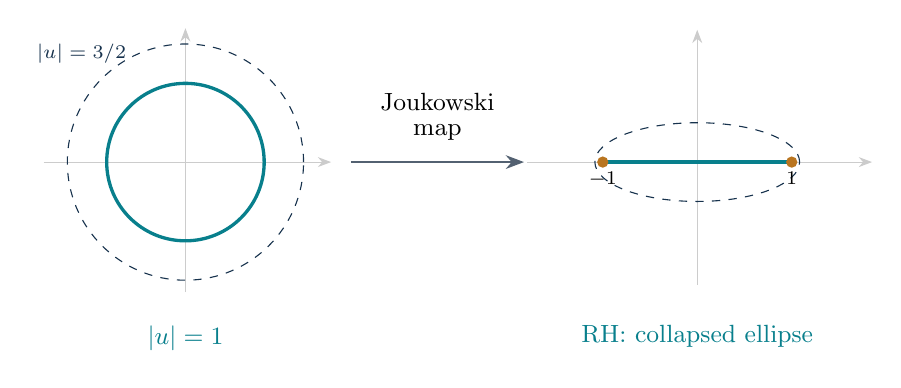
\begin{tikzpicture}[>=Stealth]
 \begin{scope}[xshift=-3.2cm]
  \draw[black!20,->](-1.8,0)--(1.85,0);
  \draw[black!20,->](0,-1.65)--(0,1.7);
  \draw[teal,very thick](0,0) circle(1);
  \draw[navy,dashed](0,0) circle(1.5);
  \node[teal,below] at(0,-1.95){\small \(|u|=1\)};
  \node[navy] at(-1.32,1.38){\scriptsize \(|u|=3/2\)};
 \end{scope}
 \draw[->,thick,inkgray](-1.1,0)--(1.1,0);
 \node[above,align=center] at(0,.15){\small Joukowski\\[-1mm]\small map};
 \begin{scope}[xshift=3.3cm,scale=1.2]
  \draw[black!20,->](-1.8,0)--(1.85,0);
  \draw[black!20,->](0,-1.3)--(0,1.4);
  \draw[navy,dashed](0,0) ellipse(1.083333 and .416667);
  \draw[teal,very thick](-1,0)--(1,0);
  \fill[gold](-1,0)circle(1.7pt);
  \fill[gold](1,0)circle(1.7pt);
  \node[below] at(-1,0){\scriptsize \(-1\)};
  \node[below] at(1,0){\scriptsize \(1\)};
  \node[teal,below] at(0,-1.62){\small RH: collapsed ellipse};
 \end{scope}
\end{tikzpicture}
\caption{The circle-to-ellipse map for the zeros. This spectral
construction is different from applying a fixed ellipse to the
prime-reciprocal phase. The dashed ellipse has semiaxes \(13/12\)
and \(5/12\), corresponding to \(|u|=3/2\).}
\end{figure}

These two ellipse constructions have opposite roles.
The physical phase ellipse of Theorem~\ref{pc:thm:energy} must keep
nonzero linear sensitivity to \(E\). The spectral ellipse above
has zero minor axis precisely when its zero is on the critical
line. Confusing the constructions would incorrectly turn a
geometric change of variables into a proof.


% Consolidated source: Prime_Reciprocal_Circles.tex, section-index 9
\section{A direct mean-square identity for the remaining bound}
\label{pc:sec:directvariance}

The unresolved arithmetic quantity can be isolated without estimating
the zeros individually. Put
\[
 R(x)=\pi(x)-\operatorname{li}(x),\quad f(x)=\frac{R(x)}x,\quad
 A(X)=\int_2^X\frac{R(t)}{t^2}\dd t,\quad
 T(X)=\int_2^X\frac{R(t)^2}{t^2}\dd t.
\]
Partial summation and Mertens' theorem give, unconditionally,
\begin{equation}\label{pc:eq:scalarAinfty}
 \begin{aligned}
 A_\infty&:=\lim_{X\to\infty}A(X)
 =\log\log2+\BP-\frac{\operatorname{li}(2)}2,\\
 E(x)&=f(x)+A(x)-A_\infty.
 \end{aligned}
\end{equation}
Numerically, \(A_\infty=-0.62759759779276793568\ldots\).
Here the prime number theorem gives \(f(x)\to0\); no RH assumption
is used in the existence of \(A_\infty\).

\begin{proposition}[Exact optimized variance]\label{pc:prop:directvariance}
For every \(X>2\),
\begin{equation}\label{pc:eq:directvariance}
 \min_{c\in\Reals}\int_2^X(E(x)-c)^2\dd x
 =T(X)-\frac{2X}{X-2}A(X)^2.
\end{equation}
Moreover, on putting \(H(X)=A_\infty-A(X)\),
\begin{equation}\label{pc:eq:directenergy}
 \int_2^X E(x)^2\dd x
 =T(X)+XH(X)^2-2A_\infty^2.
\end{equation}
Thus \(T(\infty)<\infty\) is equivalent to RH, and when it is finite,
\begin{equation}\label{pc:eq:directenergylimit}
 T(\infty)=\int_2^\infty E(x)^2\dd x+2A_\infty^2,
 \qquad 2A_\infty^2=0.78775748951050582490\ldots .
\end{equation}
\end{proposition}
\begin{proof}
For fixed \(X\), let
\(H_X(x)=\int_x^X f(t)t^{-1}\dd t=A(X)-A(x)\).
Then \(H_X'=-f/x\), \(H_X(X)=0\), and \(H_X(2)=A(X)\).
Integration by parts gives
\[
 \int_2^X(f-H_X)^2\dd x=T(X)-2A(X)^2,
 \qquad \int_2^X(f-H_X)\dd x=2A(X).
\]
Since \(E=f-H_X+A(X)-A_\infty\), subtracting the optimal constant
subtracts the square of the mean, proving \eqref{pc:eq:directvariance}.
Expanding the same identity without subtracting the mean gives
\eqref{pc:eq:directenergy}.

If \(T(\infty)<\infty\), then
\[
 XH(X)^2
 =X\left(\int_X^\infty\frac{f(t)}t\dd t\right)^2
 \le\int_X^\infty f(t)^2\dd t\longrightarrow0.
\]
Equation \eqref{pc:eq:directenergy} proves finite \(E\)-energy.
Conversely that equation and \(XH(X)^2\ge0\) bound \(T(X)\)
whenever the \(E\)-energy is finite. Theorem~\ref{pc:thm:energy}
and passage to the limit finish the proof.
\end{proof}

The subtraction in \eqref{pc:eq:directvariance} approaches the finite
number \(2A_\infty^2\). Optimizing the center therefore cannot
cancel an unbounded \(T(X)\). This identifies the missing global
mean-square estimate precisely, rather than attributing it to an
uncontrolled choice of center.


% Consolidated source: Prime_Reciprocal_Circles.tex, section-index 11
\section{Compact logarithmic filters preserve the obstruction}\label{pc:sec:filters}

The Hardy-space viewpoint suggests averaging the error before measuring its
energy. The following result identifies precisely what every fixed compact
filter preserves. Signed filters are allowed, and the conclusion does not
require their transfer functions to be zero-free.

Extend \(E(x)\) by zero for \(0<x<2\). Let \(\mu\ne0\) be a finite complex
Borel measure on \(\mathbb R\), with compact support contained in
\([a,b]\). Define
\begin{align}
 E_\mu(x)&=\int_{\mathbb R}e^{-u/2}E(xe^{-u})\dd\mu(u),
       &&x>0,\label{pc:eq:filtered-error}\\
 M_\mu(z)&=\int_{\mathbb R}e^{-zu}\dd\mu(u),
       &&z\in\mathbb C,\label{pc:eq:filter-transfer}\\
 I_\mu(X)&=\int_0^X|E_\mu(x)|^2\dd x.
       \label{pc:eq:filtered-energy}
\end{align}
Finite sums of point masses give finite linear combinations of dilations;
an integrable density of compact support gives a logarithmic averaging
filter. Neither positivity nor normalization of \(\mu\) is assumed.

\begin{theorem}[Invariance under compact logarithmic filters]
\label{pc:thm:compactfilters}
For every measure \(\mu\) specified above,
\begin{equation}\label{pc:eq:filter-rh}
 \int_0^\infty|E_\mu(x)|^2\dd x<\infty
 \quad\Longleftrightarrow\quad\RH.
\end{equation}
Moreover, the exact energy exponent is unchanged:
\begin{equation}\label{pc:eq:filter-growth}
 \boxed{\quad
 \limsup_{X\to\infty}
 \frac{\log(1+I_\mu(X))}{\log X}=2\Theta-1.
 \quad}
\end{equation}
The exponent in \eqref{pc:eq:filter-growth} is a limsup; no lower bound at
every sufficiently large \(X\) is asserted.
\end{theorem}

\begin{proof}
First, \(E_\mu(x)=0\) when \(x<2e^a\). Compact support makes
\(M_\mu\) entire. It is not identically zero: otherwise all derivatives
at zero would vanish, so
\(\int u^n\dd\mu(u)=0\) for every integer \(n\ge0\). Polynomial density
in \(C([a,b])\), together with finiteness of the total variation of
\(\mu\), would force \(\mu=0\).

For \(\Re s>1\), define the filtered Mellin transform with the full
positive-axis domain:
\[
 F_\mu(s)=\int_0^\infty E_\mu(x)x^{-s}\dd x.
\]
Since \(E\) is bounded and \(\mu\) has compact support, the relevant
integrals are absolutely convergent in this initial half-plane. Fubini's
theorem and the substitution \(x=e^uy\) give the exact identity
\begin{equation}\label{pc:eq:filtered-mellin}
 F_\mu(s)=M_\mu\left(s-\frac12\right)F(s),
 \qquad \Re s>1.
\end{equation}

Set \(f(t)=e^{t/2}E(e^t)\), using the zero extension, and let
\[
 g(t)=\int_{\mathbb R}f(t-u)\dd\mu(u).
\]
Then \(g(t)=e^{t/2}E_\mu(e^t)\), and a change of variables gives
\[
 \norm{g}_{L^2(\mathbb R)}^2
   =\int_0^\infty|E_\mu(x)|^2\dd x.
\]
Under \(\RH\), Theorem~\ref{pc:thm:energy} gives \(f\in L^2(\mathbb R)\).
Young's inequality for convolution with a finite measure yields
\[
 \norm{g}_2\le |\mu|(\mathbb R)\norm{f}_2,
\]
which proves the forward implication in \eqref{pc:eq:filter-rh}.

Conversely, suppose \(E_\mu\in L^2(0,\infty)\). The lower support bound
\(2e^a>0\) and Cauchy--Schwarz show that \(F_\mu\) is holomorphic in
\(\Re s>1/2\). Let \(\rho\) be a zero of \(\zeta\) of multiplicity
\(m_\rho\), with \(\Re\rho>1/2\). The local continuation of the Mellin
identity for \(F\) has the form
\begin{equation}\label{pc:eq:filter-local-log}
 F(s)=\frac{m_\rho}{s-1}\log(s-\rho)+H_\rho(s),
\end{equation}
where \(H_\rho\) is holomorphic near \(\rho\) and a branch of the
logarithm is chosen on a slit neighborhood. Indeed, the prime-power
correction is holomorphic for \(\Re s>1/2\), while the local factor
\(\zeta(s)=(s-\rho)^{m_\rho}h(s)\), \(h(\rho)\ne0\), gives the
displayed logarithm.

Continue the right side of \eqref{pc:eq:filtered-mellin} from its initial
half-plane along paths avoiding the isolated zeros. Continuation once
around a sufficiently small loop surrounding \(\rho\) changes its value
by
\begin{equation}\label{pc:eq:filter-monodromy}
 2\pi\ii\,m_\rho\frac{M_\mu(s-\tfrac12)}{s-1}.
\end{equation}
This is not identically zero on the neighborhood. In particular, a zero
of \(M_\mu\) of any finite order \(r\) at \(\rho-1/2\) merely replaces
the logarithmic term by a nonzero holomorphic factor times
\((s-\rho)^r\log(s-\rho)\); its monodromy remains nonzero.
Thus the product in \eqref{pc:eq:filtered-mellin} cannot agree with the
single-valued holomorphic function \(F_\mu\) throughout
\(\Re s>1/2\). There is no such zero \(\rho\), and the functional
equation gives \(\RH\).

For the growth statement, put \(A=|\mu|(\mathbb R)\), and extend
\(I(X)=\int_2^X E(x)^2\dd x\) by zero for \(0<X<2\).
Cauchy--Schwarz with respect to \(|\mu|\), followed by Tonelli's theorem,
gives
\begin{align*}
 I_\mu(X)
 &=\int_{-\infty}^{\log X}|g(t)|^2\dd t\\
 &\le A\int_{\mathbb R}
       \int_{-\infty}^{\log X-u}|f(v)|^2\dd v\dd|\mu|(u)\\
 &\le A^2 I(e^{-a}X).
\end{align*}
Theorem~\ref{pc:thm:momentgrowth} therefore implies
\[
 \Gamma_\mu:={\limsup}_{X\to\infty}
 \frac{\log(1+I_\mu(X))}{\log X}
 \le\gamma:=2\Theta-1.
\]
If \(\gamma=0\), equality follows from \(\Gamma_\mu\ge0\).
Otherwise, suppose \(\Gamma_\mu<\gamma\), and choose
\(\Gamma_\mu<\beta<\beta'<\gamma\). Then
\(I_\mu(X)=O(X^\beta)\), so integration by parts yields
\[
 \int_0^\infty x^{-\beta'}|E_\mu(x)|^2\dd x<\infty.
\]
With \(\eta=(1+\beta')/2<\Theta\), weighted Cauchy--Schwarz makes
\(F_\mu\) holomorphic in \(\Re s>\eta\). By the definition of
\(\Theta\), there is a zero \(\rho\) with \(\Re\rho>\eta\).
Here \(\eta>1/2\), so \eqref{pc:eq:filter-local-log} applies. Its surviving
monodromy contradicts holomorphy just as before. This proves
\eqref{pc:eq:filter-growth}.
\end{proof}

\begin{remark}[Scope of the obstruction]
This theorem concerns fixed, nonzero, compactly supported linear filters
of the error. It does not rule out nonlinear constructions, noncompact
operators, or new arithmetic inequalities. It shows that a filter in the
stated class cannot supply the missing uniform bound merely by cancelling
the logarithmic singularities: even a deliberately placed zero of its
entire transfer function does not cancel such a branch point.
\end{remark}


\clearpage
\part{Geometric, harmonic, and arithmetic transfers}\label{part:transfers}


% Consolidated source: Prime_Reciprocal_Circles.tex, section-index 12
\section{What positivity and Hardy-space transfers require}
\label{pc:sec:positivitytransfer}

The positive forms arising from circle variance, Weil's criterion, and
finite spectral approximations have different hypotheses. Identifying
those differences prevents an automatic positivity statement from being
used as an upper bound on arithmetic energy.

\subsection{A Gram square is not the Weil zero pairing}

Use the multiplicative Fourier convention
\[
 \widehat g(z)=\int_0^\infty g(x)x^{-\ii z}\frac{\dd x}{x},
 \qquad s_\rho=\frac{\rho-\tfrac12}{\ii}.
\]
For smooth compactly supported test functions, with the usual conditions
\(\widehat g(\pm\ii/2)=0\) removing the pole terms, the zero side of
Weil's quadratic form involves
\[
 \mathcal Q(g)=\sum_\rho
 \widehat g(s_\rho)\,
 \overline{\widehat g(\overline{s_\rho})}.
\]
Its nonnegativity for every admissible \(g\) is the Weil criterion;
see \cite[Section~4.1]{pc:connessurvey}. Under \(\RH\), each \(s_\rho\)
is real and the corresponding summand is an absolute square.

For an off-line pair \(s,\overline s\), however, put
\(a=\widehat g(s)\) and \(b=\widehat g(\overline s)\). Its contribution
is
\[
 2\Re(a\overline b)
 =\begin{pmatrix}\overline a&\overline b\end{pmatrix}
   \begin{pmatrix}0&1\\1&0\end{pmatrix}
   \begin{pmatrix}a\\b\end{pmatrix}.
\]
The displayed matrix has eigenvalues \(1\) and \(-1\). Replacing this
pairing by \(|a|^2+|b|^2\) adds exactly \(|a-b|^2\), eliminating its
negative direction. This block computation distinguishes the two forms;
it does not by itself isolate a pair from the full infinite zero sum.

By contrast, a variance such as
\[
 V_N=\min_{c\in\mathbb C}\sum_{n=2}^Nw_n|U_n-c|^2
\]
is nonnegative for every sequence \((U_n)\) and every choice of positive
weights. That automatic Gram positivity does not establish Weil
positivity, and it gives no uniform upper bound on \(V_N\) or \(D_N\).
The required arithmetic estimate remains a bound on the size of the
specific vector, rather than positivity of its squared norm.

\subsection{Noor's density result and the unbounded inverse}

Noor considers the functions
\[
 h_k(z)=\frac{1}{1-z}
       \log\left(\frac{1+z+\cdots+z^{k-1}}{k}\right),
 \qquad k\ge2.
\]
Their linear span is dense in \(H^2\) if and only if \(\RH\).
Unconditionally, the span of \((1-z)h_k\) is dense in \(H^2\), and the
span of \(h_k\) is dense for the compact-open topology
\cite[Theorems~8--10]{pc:noor}.

The missing norm control cannot be recovered by simply dividing by
\(1-z\). Indeed, the explicit polynomials
\[
 p_N(z)=\frac{1+z+\cdots+z^{N-1}}{\sqrt N}
\]
satisfy
\[
 \norm{p_N}_{H^2}=1,
 \qquad
 \norm{(1-z)p_N}_{H^2}=\sqrt{\frac2N}\longrightarrow0.
\]
Thus multiplication by \(1-z\) has no bounded inverse on its range.
Convergence after this multiplication, or convergence on every compact
subset of the disk, does not supply the boundary norm bound needed for
the prime-circle energy.

\subsection{The remaining hypotheses in the Connes approximation}

Connes' real-zero theorem applies to a lower-bounded selfadjoint operator
on a finite interval whose kernel depends on the difference of its
arguments. It concludes that the Fourier transform of its lowest
eigenfunction has only real zeros, provided that the lowest eigenvalue
is simple and isolated and the eigenfunction is even
\cite[Theorem~6.1]{pc:connessurvey}.

For the restricted Weil forms, the same paper explicitly leaves two
steps to be established: the required simplicity and evenness of the
lowest eigenfunction, and sufficiently strong approximation of
\(\theta_x\) by \(k_\lambda\)
\cite[Section~6.6]{pc:connessurvey}. Consequently, its accurate finite
approximations do not furnish a uniform bound for the present energy.
They identify a substantive spectral route, whose limiting and
positivity hypotheses still require proof.


% Consolidated source: Prime_Reciprocal_Circles.tex, section-index 13
\section{Closing the Epstein threshold calculation}
\label{pc:sec:epsteinclosure}

This section resolves a concrete claim in the proposed circle--ellipse
comparison.  The constant $4\pi e^{-\gamma}$ is an exact transition value
for an \emph{averaged} Eisenstein series, as already proved by
Lagarias--Suzuki \cite{pc:lagariassuzuki,pc:suzukinote}.  For a fixed rectangular
lattice, a positive Bessel correction survives, and the central crossing
occurs strictly below that constant.  The calculation below establishes
the correction, uniqueness, and a certified enclosure; it makes no claim
of a new criterion for the Riemann zeta function.

For $k\geq1$, initially in $\operatorname{Re}s>1$, set
\[
 Z_k(s)=\sum_{(m,n)\in\mathbb Z^2\setminus\{(0,0)\}}
              (m^2+k^2n^2)^{-s},
 \qquad k_0=4\pi e^{-\gamma},
\]
where $\gamma$ is Euler's constant.  Values outside this half-plane refer
to the meromorphic continuation.  Let $d(r)$ denote the number of
positive divisors of $r$.

\begin{proposition}[Exact central value]
\label{pc:prop:epsteincentral}
For every $k>0$,
\begin{equation}
 \Phi(k):=Z_k(1/2)
   =2\log\frac{k}{k_0}
      +8\sum_{r=1}^{\infty}d(r)K_0(2\pi kr).
 \label{pc:eq:epsteincentral}
\end{equation}
In particular, $\Phi(k_0)>0$.
\end{proposition}

\begin{proof}
The Fourier, or Chowla--Selberg, expansion
\cite{pc:lagariassuzuki} gives
\begin{align*}
 Z_k(s)={}&2\zeta(2s)
  +2\sqrt\pi\,k^{1-2s}
       \frac{\Gamma(s-1/2)}{\Gamma(s)}\zeta(2s-1)\\
 &+\frac{8\pi^s k^{1/2-s}}{\Gamma(s)}
     \sum_{r\geq1}r^{s-1/2}\sigma_{1-2s}(r)
                         K_{s-1/2}(2\pi kr),
\end{align*}
where $\sigma_u(r)=\sum_{d\mid r}d^u$.  At $s=1/2+\varepsilon$,
the first two terms are respectively
$\varepsilon^{-1}+2\gamma+O(\varepsilon)$ and
$-\varepsilon^{-1}+2\log(k/(4\pi))+O(\varepsilon)$.
Their poles cancel.  The last series converges locally uniformly and
becomes the series in \eqref{pc:eq:epsteincentral}.  Every $K_0$ term is
strictly positive.
\end{proof}

\begin{proposition}[Unique rectangular central crossing]
\label{pc:prop:epsteinunique}
There is exactly one $k_{\mathrm{rect}}\geq1$ with
$Z_{k_{\mathrm{rect}}}(1/2)=0$.  It satisfies $k_{\mathrm{rect}}<k_0$ and
\begin{equation}
 \boxed{\quad
  2.96037427750280\,10^{-19}
  <k_0-k_{\mathrm{rect}}
  <2.96037427750281\,10^{-19}.
 \quad}
 \label{pc:eq:epsteincertificate}
\end{equation}
Thus $k_{\mathrm{rect}}\approx
7.055507955448182762474611110423$, rather than exactly $k_0$.
\end{proposition}

\begin{proof}[Existence and uniqueness]
The integral representations of $K_0$ and $K_1$, together with
$1+t^2/2\leq\cosh t\leq e^{t^2/2}$, imply
\begin{equation}
 K_0(x)\leq e^{-x}\sqrt{\frac{\pi}{2x}},\qquad
 K_1(x)\leq e^{-x}\sqrt{\frac{\pi}{2(x-1)}}\quad(x>1).
 \label{pc:eq:epsteinbesselbounds}
\end{equation}
Here $\log\cosh t\leq t^2/2$ follows by integrating $\tanh t\leq t$.
Termwise differentiation in \eqref{pc:eq:epsteincentral} gives
\[
 \Phi'(k)=\frac2k-16\pi\sum_{r\geq1}r\,d(r)K_1(2\pi kr).
\]
For fixed $r\geq1$, the function
$k e^{-2\pi kr}/\sqrt{2\pi kr-1}$ decreases on $k\geq1$.
Consequently, using $d(r)\leq r$ and $q=e^{-2\pi}$,
\begin{align*}
 8\pi k\sum_{r\geq1}r\,d(r)K_1(2\pi kr)
 &\leq B:=\frac{8\pi\sqrt{\pi}}{\sqrt{2(2\pi-1)}}
                      \frac{q(1+q)}{(1-q)^3}
 <0.026,\\
 \Phi'(k)&\geq\frac{2(1-B)}k>\frac{1.948}{k}>0.
\end{align*}
Also, \eqref{pc:eq:epsteinbesselbounds} yields
\[
 \Phi(1)\leq-2\log k_0+\frac{4q}{(1-q)^2}<-3.9001.
\]
The Bessel series tends to zero as $k\to\infty$, so $\Phi(k)\to+\infty$.
Strict monotonicity proves existence and uniqueness.  Since $\Phi(k_0)>0$,
the crossing is below $k_0$.  The numerical enclosure is certified below.
\end{proof}

\begin{corollary}[A sufficient condition for real off-line zeros]
\label{pc:cor:epsteinrealzero}
If $k>k_{\mathrm{rect}}$, then $Z_k(s)$ has a real zero in $(1/2,1)$
and a reflected real zero in $(0,1/2)$.
\end{corollary}

\begin{proof}
We have $Z_k(1/2)>0$, whereas
$\operatorname{Res}_{s=1}Z_k(s)=\pi/k>0$ implies
$Z_k(s)\to-\infty$ as $s\to1^-$.  Continuity supplies the first zero.
The functional equation for
$\Lambda_k(s)=k^s\pi^{-s}\Gamma(s)Z_k(s)$ is
$\Lambda_k(s)=\Lambda_k(1-s)$, giving the reflected zero.
\end{proof}

\begin{remark}
The converse asserted for \emph{all} off-critical zeros would be
unjustified: a negative central value alone does not exclude other real
or nonreal zeros.  The proposition concerns a unique \emph{central
crossing}; the corollary gives only the stated sufficient implication.
\end{remark}

\paragraph{A finite, rigorous numerical certificate.}
For $x>0$ define
\[
 P_J(x)=\sum_{j=0}^J
       \frac{(-1)^j(2j)!^2}{32^j(j!)^3x^j}.
\]
The exact integral
\[
 K_0(x)=\frac{e^{-x}}{\sqrt{2x}}
   \int_0^\infty e^{-u}u^{-1/2}
        \left(1+\frac{u}{2x}\right)^{-1/2}\,\dd u
\]
and Taylor's theorem give, for every integer $M\geq0$,
\begin{equation}
 e^{-x}\sqrt{\frac\pi{2x}}P_{2M+1}(x)
 <K_0(x)<
 e^{-x}\sqrt{\frac\pi{2x}}P_{2M}(x).
 \label{pc:eq:epsteintaylor}
\end{equation}
Indeed, the derivatives of $(1+v)^{-1/2}$ alternate in sign for
$v\geq0$, so its Taylor remainder has the required sign; integration
then gives the displayed coefficients.  These are bounds with signed
remainders, not an assumption that an asymptotic series converges.
For $q_k=e^{-2\pi k}$, \eqref{pc:eq:epsteinbesselbounds} also gives
\begin{equation}
 0<\sum_{r\geq3}d(r)K_0(2\pi kr)
 \leq\frac{q_k^3(3-2q_k)}{2\sqrt{k}(1-q_k)^2}.
 \label{pc:eq:epsteintail}
\end{equation}
Use $P_{13}$ and $P_{12}$ for lower and upper bounds on the first
two terms, then add \eqref{pc:eq:epsteintail} only to the upper bound.
Outward interval arithmetic gives
\begin{align*}
 \Phi(k_0-2.96037427750280\,10^{-19})
       &\in[1.5398,1.5459]\,10^{-34},\\
 \Phi(k_0-2.96037427750281\,10^{-19})
       &\in[-1.2949,-1.2888]\,10^{-34}.
\end{align*}
These opposite signs and strict monotonicity prove
\eqref{pc:eq:epsteincertificate}.  The accompanying certificate evaluates
only interval constants and elementary functions; it does not rely on
a floating-point Bessel routine.

\paragraph{Why averaging gives the exact constant.}
For a sheared lattice write
\[
 Z_{x,y}(s)=\sum_{(m,n)\ne(0,0)}
           \bigl((m+xn)^2+y^2n^2\bigr)^{-s}.
\]
Its central value and horizontal average are
\begin{align*}
 Z_{x,y}(1/2)&=2\log(y/k_0)
       +8\sum_{r\geq1}d(r)\cos(2\pi rx)K_0(2\pi ry),\\
 \int_0^1 Z_{x,y}(1/2)\,\dd x&=2\log(y/k_0).
\end{align*}
Thus averaging removes precisely the correction retained by the
rectangle $x=0$.  In the standard normalization
$E^*(x+iy,s)=\frac12\pi^{-s}\Gamma(s)y^s Z_{x,y}(s)$,
the constant Fourier coefficient is
\[
 a_0(y,s)=\zeta^*(2s)y^s+\zeta^*(2-2s)y^{1-s},\qquad
 \zeta^*(w)=\pi^{-w/2}\Gamma(w/2)\zeta(w),
\]
and $a_0(y,1/2)=\sqrt y\log(y/k_0)$.
Lagarias--Suzuki proved that, for $y\geq1$, all zeros of $a_0$ lie on
the critical line except for precisely two real zeros when $y>k_0$
\cite{pc:lagariassuzuki,pc:suzukinote}.  The exact averaged threshold is
therefore established prior work.  Removing the nonconstant Fourier
terms changes the function; this averaging identity supplies no bound
on the original prime-circle discrepancy and no proof of $\RH$.


% Consolidated source: Prime_Reciprocal_Circles.tex, section-index 14
\section{Pair energies, harmonic certificates, and the original deficit}
\label{pc:m80:pairenergy}

The vectors \(U_n\), weights \(w_n\), total mass \(W_N\), and original
deficit \(D_N\) retain the definitions in
\eqref{pc:eq:U}--\eqref{pc:eq:DV}. In particular, neither the vectors nor their
weights are changed in this section. For integers \(k,m\ge1\), define
\begin{align}
 M_{k,N}&=\sum_{n=2}^Nw_nU_n^k,\qquad
 V_N^{(k)}=W_N-\frac{|M_{k,N}|^2}{W_N},
 \label{pc:m80:eq:harmonics}\\
 C_{m,N}&=\frac1{W_N}
 \sum_{2\le j<k\le N}w_jw_k|U_j-U_k|^{2m},
 \label{pc:m80:eq:pairenergy}\\
 J_{m,N}&=\sum_{n=2}^Nw_n|U_n-u_\infty|^{2m},
 \qquad u_\infty=e^{2\pi\ii\BP}.
 \label{pc:m80:eq:fixedmoment}
\end{align}
Every finite \(C_{m,N}\) uses only the original prime vectors and weights;
it requires no supplied value of \(\BP\).
The quantity \(J_{m,N}\) is used for analysis of its limit.
One has \(V_N^{(1)}=V_N\) and \(C_{1,N}=V_N\).
Higher \(m\) measure higher powers of pairwise distance, so their boundedness
must not be identified with boundedness of the original \(D_N\).

\subsection{Exact harmonic identities}

\begin{proposition}[A finite harmonic formula]
\label{pc:m80:prop:harmonicidentity}
For every integer \(m\ge1\) and every \(N\ge2\),
\begin{equation}
 \boxed{\quad
 C_{m,N}=\sum_{k=1}^m
 (-1)^{k+1}\binom{2m}{m-k}V_N^{(k)}.
 \quad}
 \label{pc:m80:eq:harmonicidentity}
\end{equation}
In particular,
\begin{align}
 C_{2,N}&=4V_N^{(1)}-V_N^{(2)},\nonumber\\
 C_{3,N}&=15V_N^{(1)}-6V_N^{(2)}+V_N^{(3)},\nonumber\\
 C_{4,N}&=56V_N^{(1)}-28V_N^{(2)}
             +8V_N^{(3)}-V_N^{(4)}\ge0.
 \label{pc:m80:eq:fourharmonics}
\end{align}
\end{proposition}
\begin{proof}
The binomial expansion gives
\[
 |1-e^{\ii t}|^{2m}
 =\binom{2m}{m}
  +2\sum_{k=1}^m(-1)^k\binom{2m}{m-k}\cos(kt).
\]
Evaluating at \(t=0\) and subtracting rewrites this as
\[
 |1-e^{\ii t}|^{2m}
 =2\sum_{k=1}^m(-1)^{k+1}
       \binom{2m}{m-k}\{1-\cos(kt)\}.
\]
For \(U_j=e^{\ii\phi_j}\), expansion of \(|M_{k,N}|^2\) gives
\[
 V_N^{(k)}
 =\frac2{W_N}\sum_{j<\ell}w_jw_\ell
              \{1-\cos(k(\phi_j-\phi_\ell))\}.
\]
Substitution proves the identity, including its normalization.
Nonnegativity follows from the pair definition, even though the
harmonic coefficients have alternating signs.
\end{proof}

\subsection{A general limit theorem for convergent directions}

\begin{theorem}[Pair moments and the limiting direction]
\label{pc:m80:thm:pairlimit}
Let \(u_n\) be any unit complex numbers with \(u_n\to u_\infty\), and
let \(w_n>0\) with \(W_N=\sum_{n=2}^Nw_n\to\infty\).
For an integer \(m\ge1\), define \(C_{m,N},J_{m,N}\) as in
\eqref{pc:m80:eq:pairenergy}--\eqref{pc:m80:eq:fixedmoment}, using \(u_n\).
Then
\begin{equation}
 0\le C_{m,N}\le 2^{2m-1}J_{m,N},
 \label{pc:m80:eq:pairupper}
\end{equation}
and the extended-real limit satisfies
\begin{equation}
 \lim_{N\to\infty}C_{m,N}
 =J_{m,\infty}:=\sum_{n=2}^{\infty}w_n|u_n-u_\infty|^{2m}
 \ \in[0,\infty].
 \label{pc:m80:eq:pairlimit}
\end{equation}
Consequently,
\begin{equation}
 \sup_N C_{m,N}<\infty
 \quad\Longleftrightarrow\quad J_{m,\infty}<\infty .
 \label{pc:m80:eq:pairbounded}
\end{equation}
No restriction on the relative sizes of the weights is needed here.
\end{theorem}
\begin{proof}
Put \(q=2m\) and \(d_n=|u_n-u_\infty|^q\).
The triangle inequality and convexity give
\[
 |u_j-u_k|^q\le 2^{q-1}(d_j+d_k).
\]
As
\[
 \sum_{j<k}w_jw_k(d_j+d_k)
 =\sum_jw_jd_j(W_N-w_j)\le W_NJ_{m,N},
\]
this proves \eqref{pc:m80:eq:pairupper}.

Fix an index \(L\). Split the pair sum into pairs within
\(\{2,\ldots,L\}\), pairs with one index in this set, and pairs with
both indices larger than \(L\). The first part, divided by \(W_N\),
tends to zero. For each fixed \(j\le L\), weighted Cesaro convergence
gives
\[
 \frac1{W_N}\sum_{k=L+1}^Nw_k|u_j-u_k|^q
 \longrightarrow |u_j-u_\infty|^q.
\]
Indeed the summand tends to the displayed limit, is bounded, and
\((W_N-W_L)/W_N\to1\). The cross-pair part therefore tends to
\(J_{m,L}\). All remaining terms are nonnegative, so
\[
 \liminf_{N\to\infty}C_{m,N}\ge J_{m,L}.
\]
If \(J_{m,\infty}=\infty\), letting \(L\to\infty\) proves divergence
of \(C_{m,N}\) to infinity.

Suppose instead that \(J_{m,\infty}<\infty\). Applying the same
triangle inequality to the pairs entirely in the tail gives
\[
 \frac1{W_N}
 \sum_{L<j<k\le N}w_jw_k|u_j-u_k|^q
 \le
 2^{q-1}\frac{W_N-W_L}{W_N}
       \sum_{n=L+1}^Nw_nd_n
 \le2^{q-1}(J_{m,\infty}-J_{m,L}).
\]
Consequently,
\[
 J_{m,L}\le\liminf_N C_{m,N}
 \le\limsup_N C_{m,N}
 \le J_{m,L}+2^{q-1}(J_{m,\infty}-J_{m,L}).
\]
Letting \(L\to\infty\) proves the finite-limit assertion.
The equivalence follows either from these limits and
\eqref{pc:m80:eq:pairupper}, or directly from the two estimates.
\end{proof}

\subsection{Sampling every even moment at prime endpoints}

\begin{lemma}[An elementary interpolation bound]
\label{pc:m80:lem:interpolation}
For every \(q>0\) and \(a,b\in\mathbb R\),
\begin{equation}
 \frac{|a|^q+|b|^q}{2(q+1)}
 \le\int_0^1|(1-y)a+yb|^q\dd y
 \le |a|^q+|b|^q .
 \label{pc:m80:eq:interpolation}
\end{equation}
\end{lemma}
\begin{proof}
The upper bound follows because the absolute value of a point on
the segment is at most \(\max(|a|,|b|)\).
For the lower bound, set \(r=|a|\) and \(t=|b|\).
The reverse triangle inequality shows that the integral is at least
the integral with endpoints \(r,-t\). If \(r+t>0\), the latter is
\[
 \frac{r^{q+1}+t^{q+1}}{(q+1)(r+t)}.
\]
The inequality
\[
 2(r^{q+1}+t^{q+1})-(r+t)(r^q+t^q)
 =(r-t)(r^q-t^q)\ge0
\]
proves the claim. The case \(r=t=0\) is immediate.
\end{proof}

\begin{proposition}[Prime sampling for every \(q>1\)]
\label{pc:m80:prop:sampling}
For fixed \(q>1\), put
\[
 I_q(X)=\int_2^X|E(x)|^q\dd x,\qquad
 A_{q,N}=\sum_{n=2}^Nw_n|E(p_n)|^q .
\]
Then
\begin{equation}
 I_q(p_N)\ll_q1+A_{q,N}\ll_q1+I_q(p_{N+1}).
 \label{pc:m80:eq:sampling}
\end{equation}
In particular, for \(q=2m\), replacing \(A_{q,N}\) by \(J_{m,N}\)
preserves both these comparisons and the corresponding convergence
criterion.
\end{proposition}
\begin{proof}
Use the existing notation \(e_n=E(p_n)\),
\(h_n=p_{n+1}-p_n\), and
\(b_n=E(p_{n+1}^-)=e_{n+1}-1/p_{n+1}\).
On a prime gap, the change of variable
\[
 y=\frac{\log\log x-\log\log p_n}
          {\log\log p_{n+1}-\log\log p_n}
\]
gives \(E(x)=(1-y)e_n+yb_n\).
As in Lemma~\ref{pc:lem:gap}, Bertrand's postulate bounds the ratio of
the largest and smallest values of \(\dd x/\dd y\) by \(4\).
Its integral is \(h_n\), so \(\dd x/\dd y\ge h_n/4\).
Lemma~\ref{pc:m80:lem:interpolation} and the pointwise upper bound give
\begin{equation}
 \frac{h_n}{8(q+1)}(|e_n|^q+|b_n|^q)
 \le\int_{p_n}^{p_{n+1}}|E(x)|^q\dd x
 \le h_n(|e_n|^q+|b_n|^q).
 \label{pc:m80:eq:gapq}
\end{equation}
The jump correction is summable:
\begin{equation}
 \sum_{n\ge1}\frac{h_n}{p_{n+1}^{q}}
 \le\int_2^\infty x^{-q}\dd x
 =\frac{2^{1-q}}{q-1}<\infty .
 \label{pc:m80:eq:jumpq}
\end{equation}
The inequalities
\[
 |x+y|^q\le2^{q-1}(|x|^q+|y|^q)
\]
applied in both directions permit replacement of \(b_n\) by
\(e_{n+1}\). Summing \eqref{pc:m80:eq:gapq} through \(n=N-1\)
proves the left comparison in \eqref{pc:m80:eq:sampling}; summing
through \(n=N\) proves the right comparison. The initial endpoint
and \eqref{pc:m80:eq:jumpq} contribute only constants.

Finally,
\[
 |U_n-u_\infty|
 =2|\sin(\pi E(p_n))|
 \sim2\pi|E(p_n)|
\]
as \(n\to\infty\), with the usual interpretation when an endpoint
value is zero. Thus the \(q\)-th powers are comparable on a tail;
the finitely many initial terms are absorbed by the constants.
\end{proof}

\begin{corollary}[The exact boundedness threshold]
\label{pc:m80:cor:threshold}
For the original prime vectors and weights and every integer \(m\ge1\),
\begin{equation}
 \boxed{\quad
 \sup_N C_{m,N}<\infty
 \quad\Longleftrightarrow\quad
 \Theta\le1-\frac1{2m}.
 \quad}
 \label{pc:m80:eq:threshold}
\end{equation}
At every finite case the limit is exactly
\[
 \lim_N C_{m,N}
 =\sum_{n=2}^\infty
   w_n|e^{2\pi\ii E(p_n)}-1|^{2m}.
\]
\end{corollary}
\begin{proof}
Combine Theorem~\ref{pc:m80:thm:pairlimit},
Proposition~\ref{pc:m80:prop:sampling}, and the endpoint-inclusive
integrability criterion in Theorem~\ref{pc:thm:Lq}.
\end{proof}

\subsection{Moving centers and exact growth}

\begin{lemma}[A moving-center estimate for pair moments]
\label{pc:m80:lem:moving}
In the setting of Theorem~\ref{pc:m80:thm:pairlimit}, suppose in addition
that \(W_{N+1}\le\Lambda W_N\) for some fixed \(\Lambda\) and all
sufficiently large \(N\). If \(0\le a<1\) and
\(C_{m,N}=O(W_N^a)\), then
\begin{equation}
 J_{m,N}=O(W_N^a).
 \label{pc:m80:eq:moving}
\end{equation}
\end{lemma}
\begin{proof}
Write \(q=2m\) and \(m_N=W_N^{-1}\sum_{n=2}^Nw_nu_n\).
Convexity and Jensen's inequality give
\begin{equation}
 \sum_{n=2}^Nw_n|u_n-m_N|^q
 \le\frac1{W_N}\sum_{j,k=2}^Nw_jw_k|u_j-u_k|^q
 =2C_{m,N}.
 \label{pc:m80:eq:jensen}
\end{equation}
If \(M>N\), a second application of Jensen on the first \(N\) terms
yields
\[
 W_N|m_N-m_M|^q
 \le\sum_{n=2}^Nw_n|u_n-m_M|^q
 \le2C_{m,M}.
\]
Starting at a sufficiently large \(N_0=N\), let \(N_{j+1}\) be the
first index with \(W_{N_{j+1}}\ge2W_{N_j}\). The bounded-overshoot
hypothesis implies
\[
 2W_{N_j}\le W_{N_{j+1}}\le2\Lambda W_{N_j}.
\]
Hence
\[
 |m_{N_{j+1}}-m_{N_j}|
 \ll W_{N_j}^{(a-1)/q}
 \le W_N^{(a-1)/q}2^{j(a-1)/q}.
\]
The series converges because \(a<1\). Weighted Cesaro convergence
gives \(m_{N_j}\to u_\infty\), so telescoping proves
\[
 |m_N-u_\infty|\ll W_N^{(a-1)/q}.
\]
Finally, \eqref{pc:m80:eq:jensen} and the power triangle inequality give
\[
 J_{m,N}
 \le2^{q-1}
 \left\{2C_{m,N}+W_N|m_N-u_\infty|^q\right\}
 \ll W_N^a.
\]
Finite initial indices cause no difficulty.
\end{proof}

\begin{theorem}[The pair energy detects its exact zero boundary]
\label{pc:m80:thm:growth}
For every integer \(m\ge1\),
\begin{equation}
 \boxed{\quad
 \limsup_{N\to\infty}
 \frac{\log(1+C_{m,N})}{\log p_N}
 =\max\{0,\,1-2m(1-\Theta)\}.
 \quad}
 \label{pc:m80:eq:growth}
\end{equation}
\end{theorem}
\begin{proof}
Proposition~\ref{pc:m80:prop:sampling},
Theorem~\ref{pc:thm:momentgrowth}, and
\(p_{N+1}<2p_N\) show that \(J_{m,N}\) has the exponent
\[
 \kappa_m=\max\{0,\,1-2m(1-\Theta)\}.
\]
Indeed the two sampling cutoffs are within a fixed factor, so
monotonicity of the integral also identifies its exponent along
prime cutoffs. The upper bound for \(C_{m,N}\) follows from
\eqref{pc:m80:eq:pairupper}.

If \(\kappa_m=0\), nonnegativity proves the result.
Otherwise \(0<\kappa_m\le1\). Were the asserted lower bound false,
choose \(a\) strictly between the actual limsup and \(\kappa_m\).
Then \(0\le a<1\) and \(C_{m,N}=O(p_N^a)=O(W_N^a)\).
The formula \(W_N=p_N+p_{N+1}-5\) and Bertrand's postulate give
both \(W_N\asymp p_N\) and bounded successive ratios.
Lemma~\ref{pc:m80:lem:moving} would imply \(J_{m,N}=O(p_N^a)\),
contradicting its already identified exponent.
\end{proof}

\subsection{A conditional four-harmonic bound and a bound for \(D_N\)}

\begin{corollary}[Four-harmonic boundedness under $(H_b)$]
\label{pc:m80:cor:fourclosure}
Admit the external zero-boundary theorem
\(\Theta\le b_*\) stated in \eqref{pc:eq:bstar} and
\cite[Theorem~27.1]{pc:liuquasi}. Since \(b_*<7/8\),
\begin{equation}
 \sup_N\left(
 56V_N^{(1)}-28V_N^{(2)}+8V_N^{(3)}-V_N^{(4)}
 \right)<\infty.
 \label{pc:m80:eq:fourclosure}
\end{equation}
The expression is nonnegative for every \(N\), and its limit is
\(J_{4,\infty}\). This consequence is conditional on $(H_b)$; it does not separately assume \(\RH\).
It retains the original weights and removes the need to supply
\(\BP\), but it is a higher-order statistic rather than \(D_N\).
\end{corollary}
\begin{proof}
Theorem~\ref{pc:thm:fixedstripclosure} gives \(E\in L^8\).
Now apply Proposition~\ref{pc:m80:prop:sampling},
Theorem~\ref{pc:m80:thm:pairlimit}, and
\eqref{pc:m80:eq:fourharmonics}.
Alternatively, use Corollary~\ref{pc:m80:cor:threshold} directly.
\end{proof}

\begin{proposition}[A finite H\"older bridge to the original deficit]
\label{pc:m80:prop:holderbridge}
For every integer \(m\ge1\) and every \(N\ge2\),
\begin{equation}
 \boxed{\quad
 D_N\le V_N
 \le\left(\frac{W_N}{2}\right)^{1-1/m}C_{m,N}^{1/m}.
 \quad}
 \label{pc:m80:eq:holderbridge}
\end{equation}
In particular, the right side with \(m=4\) is computable from four
harmonic resultants by \eqref{pc:m80:eq:fourharmonics}.
A uniform bound on that fourth pair moment yields
\(D_N=O(W_N^{3/4})\), not a uniform constant bound.
\end{proposition}
\begin{proof}
Give each unordered pair \((j,k)\) mass \(w_jw_k/W_N\).
The total mass of this positive measure is
\[
 \frac{W_N^2-\sum_{n=2}^Nw_n^2}{2W_N}\le\frac{W_N}{2}.
\]
Its integrals of \(|U_j-U_k|^2\) and
\((|U_j-U_k|^2)^m\) are respectively \(V_N\) and \(C_{m,N}\).
H\"older's inequality proves the assertion when \(m>1\).
For \(m=1\) it is the identity \(C_{1,N}=V_N\);
the zero-pair case also satisfies the displayed inequality.
\end{proof}

\begin{remark}[Nonmonotonicity]
\label{pc:m80:rem:nonmonotone}
Higher pair moments need not be nondecreasing, even though their
extended-real limits always exist for convergent directions.
With unit weights and the first two points
\(u_1=e^{\ii\pi/3},u_2=e^{-\ii\pi/3}\), one has
\(C_{2,2}=9/2\). Appending \(u_3=1\) gives
\(C_{2,3}=11/3\). This independent example uses indices starting at
\(1\). It can be extended to a convergent sequence by setting all
subsequent points equal to \(1\).
\end{remark}

\subsection{Deficits of positive-definite Fourier kernels}

Positive-definite kernels supply nonnegative expressions, but a
uniform upper budget is a separate requirement. The next result
identifies exactly what positive combinations of harmonic variances
retain.

\begin{theorem}[Coercivity of positive harmonic combinations]
\label{pc:m80:thm:positivekernel}
Let \(a_k\ge0\) satisfy
\[
 0<A_2:=\sum_{k=1}^\infty a_kk^2<\infty.
\]
Define
\[
 K_{\mathbf a}(t)=\sum_{k\ge1}a_k\cos(kt),\qquad
 Q_{\mathbf a}(t)=K_{\mathbf a}(0)-K_{\mathbf a}(t),\qquad
 \mathfrak C_N(\mathbf a)=\sum_{k\ge1}a_kV_N^{(k)}.
\]
For any convergent unit-vector sequence and positive weights with
\(W_N\to\infty\), there exist \(c>0,C_0<\infty\) such that
\begin{equation}
 cV_N-C_0\le\mathfrak C_N(\mathbf a)\le A_2V_N
 \qquad\text{for all }N.
 \label{pc:m80:eq:positivecomparison}
\end{equation}
Consequently, for the prime-circle sequence,
\begin{equation}
 \sup_N\mathfrak C_N(\mathbf a)<\infty
 \quad\Longleftrightarrow\quad \sup_ND_N<\infty
 \quad\Longleftrightarrow\quad\RH,
 \label{pc:m80:eq:positiveequivalence}
\end{equation}
and its logarithmic growth exponent is \(2\Theta-1\).
\end{theorem}
\begin{proof}
The inequality \(|z^k-w^k|\le k|z-w|\) for unit \(z,w\)
implies \(V_N^{(k)}\le k^2V_N\), proving the upper bound and
convergence of the defining series.
The exact pair formula is
\[
 \mathfrak C_N(\mathbf a)
 =\frac1{W_N}\sum_{i,j=2}^Nw_iw_j
                  Q_{\mathbf a}(\phi_i-\phi_j),
 \qquad u_n=e^{\ii\phi_n}.
\]
For \(t\ne0\) sufficiently close to zero,
\[
 0\le\frac{1-\cos(kt)}{1-\cos t}\le k^2,\qquad
 \frac{1-\cos(kt)}{1-\cos t}\longrightarrow k^2.
\]
Dominated convergence in \(k\) therefore gives
\[
 \frac{Q_{\mathbf a}(t)}{1-\cos t}\longrightarrow A_2.
\]
Choose a tail of the convergent directions on which all pairwise
phase differences lie in an arc where
\(Q_{\mathbf a}(t)\ge c(1-\cos t)\), with \(c=A_2/2\).
Let \(A\) be the total weight of the omitted finite prefix.
In the ordered-pair formula for \(V_N\), pairs with at least one
endpoint in that prefix contribute at most \(4A\), since
\(1-\cos t\le2\).
All terms of \(Q_{\mathbf a}\) are nonnegative, so
\[
 \mathfrak C_N(\mathbf a)\ge c(V_N-4A).
\]
The same lower inequality is harmless before the end of the prefix.
Take \(C_0=4cA\). The equivalence follows from
Theorem~\ref{pc:thm:deficit}; the exponent follows from
\eqref{pc:m80:eq:positivecomparison} and
Theorem~\ref{pc:thm:ThetaD}.
\end{proof}

\begin{remark}[The exact certificate still required]
\label{pc:m80:rem:certificate}
The kernel \(K_{\mathbf a}\) is positive definite;
\(Q_{\mathbf a}=K_{\mathbf a}(0)-K_{\mathbf a}\) is a conditionally
negative definite variogram, not a positive-definite kernel.
For a nonzero finite family \(a_k\ge0\), a sufficient arithmetic
certificate for the original goal is
\[
 \sum_{k=1}^ma_k\{W_N^2-|M_{k,N}|^2\}\le CW_N
 \quad\text{for every }N,
\]
with one finite \(C\).
The theorem would then give \(D_N\le(C+C_0)/c\).
Positive definiteness supplies nonnegativity of the expression;
it does not supply this upper bound. The theorem does not exclude
finding such a certificate using additional arithmetic information.
The alternating combination in \eqref{pc:m80:eq:fourharmonics} lies
outside the nonnegative-coefficient cone and has higher vanishing
order at coincident points.
\end{remark}

\begin{remark}[A precise limit of positivity alone]
\label{pc:m80:rem:counterexample}
Consider the independent sequence
\(u_n=e^{\ii n^{-1/4}}\), \(n\ge1\), with unit weights.
It converges to \(1\), and
\(\sum_n|u_n-1|^8<\infty\), so its fourth pair moment is bounded.
Every finite moment matrix of its positive atomic measure is
positive semidefinite. Nevertheless its ordinary deficit satisfies
\[
 N-\left|\sum_{n=1}^Ne^{\ii n^{-1/4}}\right|
 \sim\frac19\sqrt N.
\]
Indeed the real and imaginary parts of the sum are respectively
\[
 N-\sqrt N+O(\log N),
 \qquad \frac43N^{3/4}+O(N^{1/4}),
\]
and expansion of its modulus gives the stated asymptotic.
Thus convergence, moment-matrix positivity, and a bounded fourth
pair moment alone do not imply a bounded ordinary deficit.
This is not a counterexample to the actual prime-circle assertion.
\end{remark}

\subsection{An exact Voronoi interpretation and finite bending}

\begin{proposition}[The original weights as Voronoi lengths]
\label{pc:m80:prop:voronoi}
For \(n\ge2\), let
\[
 I_n=\left[\frac{p_{n-1}+p_n}{2},
           \frac{p_n+p_{n+1}}{2}\right].
\]
Then \(|I_n|=w_n/2\).
Let \(\Gamma\) be the polygonal curve whose derivative equals \(U_n\)
on the interior of \(I_n\), with \(\Gamma(5/2)=0\).
On the union of the first \(N-1\) cells its length is \(W_N/2\),
and its endpoint is \(M_N/2\). Consequently,
\begin{equation}
 D_N=2\{\text{length of this curve}
             -\text{distance between its endpoints}\}.
 \label{pc:m80:eq:voronoi}
\end{equation}
\end{proposition}
\begin{proof}
The cells are adjacent and their lengths telescope.
Since \(|U_n|=1\), their lengths are also the lengths of the
corresponding curve segments. Integrating the tangent gives
\(\sum_{n=2}^N|I_n|U_n=M_N/2\).
\end{proof}

\begin{proposition}[Unconditional finite bending of an interpolation]
\label{pc:m80:prop:bending}
Let \(A:[3,\infty)\to\mathbb R\) be linear on every prime gap and
take the values
\[
 A(p_n)=S(p_n)-\log\log p_n\qquad(n\ge2).
\]
Then
\begin{equation}
 \int_3^\infty|A'(x)|^2\dd x<\infty,
 \qquad
 \int_3^\infty
 \left|\frac{\dd}{\dd x}e^{2\pi\ii A(x)}\right|^2\dd x<\infty.
 \label{pc:m80:eq:bending}
\end{equation}
These statements are unconditional and concern almost-everywhere
derivatives of continuous, locally absolutely continuous functions.
\end{proposition}
\begin{proof}
On a gap with endpoints \(p<r\) and length \(h=r-p\),
\[
 \Delta A=\frac1r-\log\!\left(\frac{\log r}{\log p}\right),
 \qquad
 |\Delta A|\le\frac1r+\frac{h}{p\log p}.
\]
Thus the contribution to the first integral is
\[
 \frac{|\Delta A|^2}{h}
 \le\frac2{r^2h}+\frac{2h}{p^2(\log p)^2}.
\]
The first series converges by \(h\ge1\).
For the second, Bertrand's bound \(r<2p\) gives a uniform
comparison of \(x^{-2}(\log x)^{-2}\) with its endpoint values.
Summing over disjoint gaps therefore compares it with
\(\int_3^\infty x^{-2}(\log x)^{-2}\dd x<\infty\).
Finally, the squared derivative of the phase interpolation is
\(4\pi^2|A'(x)|^2\) almost everywhere.
\end{proof}

This continuous interpolation is distinct from the piecewise-constant
tangent field in Proposition~\ref{pc:m80:prop:voronoi}.
Finite bending does not by itself bound the length excess in
\eqref{pc:m80:eq:voronoi}. On an unbounded interval there is no
unweighted Poincare inequality of the needed form:
\(f(x)=x^{-1/4}\) tends to zero and has \(f'\in L^2([3,\infty))\),
while \(f\notin L^2([3,\infty))\).
A geometric regularity argument must therefore supply its missing
coercive estimate before it can close the original \(D_N\) target.


% Consolidated source: Prime_Reciprocal_Circles.tex, section-index 15
\section{Orthogonal polynomials and Toeplitz determinants}
\label{pc:m80:toeplitz}

The orthogonal-polynomial and determinant methods in items 11--18 of
Appendix~\ref{pc:m80:audit} lead to two different constructions. The first
uses the original atomic prime measure and yields a hierarchy of bounded
extremal polynomial norms. The second uses finite Laguerre polynomials
and gives an exact determinant formulation of the original quadratic
problem. Neither construction identifies the prime measure with a
random-matrix ensemble.

\subsection{A monotone hierarchy on the original prime measure}

For an integer \(m\ge1\), define
\begin{equation}\label{pc:m80:Hdef}
 H_{m,N}=\inf_{P(z)=z^m+\sum_{j=0}^{m-1}c_jz^j}
             \sum_{n=2}^Nw_n|P(U_n)|^2.
\end{equation}
All coefficients in this finite minimization are computed from the
original \(U_n\) and \(w_n\); the limiting direction is not an input.
These are the monic orthogonal-polynomial norms associated with the
positive atomic measure \(\sum_{n=2}^Nw_n\delta_{U_n}\).

\begin{theorem}[Extremal polynomial hierarchy]\label{pc:m80:OPUC}
Let \(u_n\to u_\infty\) be unit complex numbers, let \(w_n>0\),
and suppose \(W_N=\sum_{n=2}^Nw_n\to\infty\). Define \(H_{m,N}\)
by \eqref{pc:m80:Hdef} with \(U_n=u_n\). Then \(H_{m,N}\) is
nondecreasing in \(N\), and
\begin{equation}\label{pc:m80:OPUCcriterion}
 \sup_N H_{m,N}<\infty
 \quad\Longleftrightarrow\quad
 \sum_{n\ge2}w_n|u_n-u_\infty|^{2m}<\infty.
\end{equation}
For the prime sequence this is equivalent to
\(\Theta\le1-1/(2m)\).
\end{theorem}
\begin{proof}
Adding a nonnegative term before taking the infimum proves monotonicity.
The polynomial \((z-u_\infty)^m\) proves the implication from right to
left. Suppose conversely that all the infima are bounded by \(C\).
If the sequence has fewer than \(m\) distinct values, convergence forces
it to be eventually constant, so the required series is finite.
Otherwise fix \(m\) distinct values occurring at finite indices.
For all sufficiently large \(N\), a minimizing polynomial exists:
the quadratic objective is coercive in the lower coefficients because
evaluation at those \(m\) points has an invertible Vandermonde matrix.
Each of its values there is bounded by \(\sqrt{C/w_n}\). The same
matrix therefore bounds all the lower coefficients uniformly in \(N\).
A subsequence converges to a monic degree-\(m\) polynomial \(P\).
For each fixed finite prefix, pass to the limit in its energy and then
let the prefix grow. This gives \(\sum w_n|P(u_n)|^2\le C\).

If \(P(u_\infty)\ne0\), the summands have a positive lower factor
on the tail, contradicting \(W_N\to\infty\). Thus
\(P(z)=(z-u_\infty)^rQ(z)\), where \(1\le r\le m\) and
\(Q(u_\infty)\ne0\). On a tail, \(|Q(u_n)|\) is bounded below,
so the \(2r\)-moment is finite. Since \(|u_n-u_\infty|\le2\),
the \(2m\)-moment is also finite. The prime assertion follows from
the sampled moment criterion in Section~\ref{pc:m80:pairenergy}.
\end{proof}

Put
\[
 G_{r,N}=\left(\sum_{n=2}^Nw_nU_n^{j-k}\right)_{0\le j,k<r}.
\]
This is a positive semidefinite Toeplitz Gram matrix. The Schur
complement formula for monic least squares gives
\begin{equation}\label{pc:m80:Gramratio}
 H_{m,N}=\frac{\det G_{m+1,N}}{\det G_{m,N}}
 \qquad\text{whenever }G_{m,N}\text{ is invertible}.
\end{equation}
Invertibility means that at least \(m\) distinct sampled values have
occurred. Before that, a monic polynomial can vanish on the support,
but the corresponding ratio may be \(0/0\); it must not be used.
The orientation of the Gram entries only transposes the more usual
moment convention and leaves determinants unchanged. In particular,
\[
 H_{1,N}=V_N,\qquad
 D_N=\lambda_{\min}(G_{2,N}),\qquad
 \det G_{2,N}=W_NV_N.
\]
Positive semidefiniteness alone is automatic for any positive measure
and does not give an upper bound for its smallest eigenvalue.

\begin{corollary}[A bounded degree-four extremal norm]
\label{pc:m80:H4}
Using the separately identified zero-free theorem in
Section~\ref{pc:sec:zerofreeclosure},
\[
 \sup_N H_{4,N}<\infty.
\]
Consequently the ratio \(\det G_{5,N}/\det G_{4,N}\) is uniformly
bounded over the indices at which its denominator is nonzero.
The same assertion for \(H_{1,N}\) remains equivalent to RH.
\end{corollary}

\subsection{Dirichlet energy and a double-index Szeg\H{o} criterion}
\label{pc:m80:dirichlet}

Fix \(\alpha>1/2\), and let \(a_n=a_n^{(\alpha)}\) be the
unconditionally defined coefficients in \eqref{pc:eq:coeff}. For each
finite \(M\ge0\), set
\begin{equation}\label{pc:m80:gpoly}
 g_M(z)=\sum_{n=0}^M\frac{a_n}{\sqrt{n+1}}z^{n+1},
 \qquad L_M(e^{it})=2\operatorname{Re}g_M(e^{it}).
\end{equation}
Only finite polynomials are used here. Assuming in advance that the
corresponding infinite series is holomorphic throughout the disk would
conflict with the radius obstruction in Theorem~\ref{pc:thm:radius}.

\begin{proposition}[Exact disk and boundary energies]
\label{pc:m80:Dirichlet}
With \(dA\) denoting ordinary planar area,
\begin{align}
 \mathcal D(g_M)
 &:=\frac1\pi\int_{\Disk}|g'_M(z)|^2\dd A(z)
   =\sum_{n=0}^M|a_n|^2,\label{pc:m80:Ddisk}\\
 &=\frac1{4\pi^2}\int_0^{2\pi}\int_0^{2\pi}
 \frac{|g_M(e^{it})-g_M(e^{is})|^2}
 {|e^{it}-e^{is}|^2}\dd t\dd s.\label{pc:m80:Dboundary}
\end{align}
Thus \(\sup_M\mathcal D(g_M)<\infty\) if and only if RH.
For every conformal bijection \(\phi:\Disk\to\Omega\),
\[
 \frac1\pi\int_\Omega
 |(g_M\circ\phi^{-1})'(w)|^2\dd A(w)=\mathcal D(g_M).
\]
\end{proposition}
\begin{proof}
Angular orthogonality and radial integration give
\(\pi^{-1}\int_\Disk| (z^k)'|^2\dd A=k\).
For the boundary formula, simultaneous rotation of \(t,s\) eliminates
cross terms of different degrees. For a degree \(k\) monomial,
\((e^{ikt}-e^{iks})/(e^{it}-e^{is})\) is a sum of \(k\)
orthogonal monomials on the two-torus, so its normalized square integral
is \(k\). The coefficient criterion, Theorem~\ref{pc:thm:coeff}, gives
the equivalence. In the change of variables \(w=\phi(z)\), the
derivative factor and the area Jacobian cancel exactly.
\end{proof}

For a positive symbol \(w\) on the unit circle write
\[
 \widehat w(k)=\frac1{2\pi}\int_0^{2\pi}w(e^{it})e^{-ikt}\dd t,
 \qquad T_L(w)=(\widehat w(j-k))_{0\le j,k<L},\quad L\ge1.
\]
The following is an application of the strong Szeg\H{o} theorem,
in the smooth real-symbol case. A primary proof and the sharp general
form are given by Simon~\cite{pc:m80simon}.

\begin{theorem}[A two-parameter determinant criterion]
\label{pc:m80:Szego}
For every finite \(M\),
\begin{equation}\label{pc:m80:Szegolimit}
 \lim_{L\to\infty}\log\det T_L(e^{L_M})
       =\sum_{n=0}^M|a_n|^2.
\end{equation}
Moreover the determinants are nondecreasing in \(L\), and hence
\begin{equation}\label{pc:m80:Szegosup}
 \boxed{\quad
 \sup_{M\ge0,\ L\ge1}\log\det T_L(e^{L_M})
       =\sum_{n\ge0}|a_n|^2.
 \quad}
\end{equation}
The equality holds in the extended nonnegative real numbers.
Finiteness is equivalent to RH; when finite its value is
\(\int_2^\infty E(x)^2\dd x\).
\end{theorem}
\begin{proof}
The symbol \(L_M\) is a real trigonometric polynomial, its mean is
zero, and its positive Fourier coefficients are
\(\widehat L_M(k)=a_{k-1}/\sqrt{k}\), \(1\le k\le M+1\).
The strong Szeg\H{o} theorem therefore gives
\[
 \lim_{L\to\infty}\det T_L(e^{L_M})
 =\exp\left(\sum_{k=1}^{M+1}k|\widehat L_M(k)|^2\right),
\]
which is \eqref{pc:m80:Szegolimit}.

For completeness, monotonicity here follows from a finite extremal
argument; it is not an interchange of limits. The ratio of successive
Gram determinants is the least norm squared of a monic degree-\(L\)
polynomial in \(L^2(e^{L_M}\dd t/(2\pi))\). Jensen's inequality
and factorization of a monic polynomial \(P(z)=\prod(z-r_j)\) give
\[
 \log\int_0^{2\pi}|P(e^{it})|^2e^{L_M(e^{it})}\frac{\dd t}{2\pi}
 \ge 2\sum_j\log\max(1,|r_j|)\ge0.
\]
Zeros on the circle cause integrable logarithmic singularities and
are handled by a limit. Thus each determinant ratio is at least one;
also \(\det T_1(e^{L_M})\ge1\). Taking the supremum in \(L\)
and then in \(M\) proves \eqref{pc:m80:Szegosup} without assuming an
infinite symbol exists. The coefficient theorem and its Parseval
identity finish the proof.
\end{proof}

The theorem transfers methods 16--17 exactly, and connects them with
the conformal methods 47 and 68--70. It does not give a common upper
bound in \(M\). Each finite symbol has its own finite Szeg\H{o}
constant; the supremum of those constants is the original unknown
energy. In particular, compact-open convergence is insufficient:
\(z^m\to0\) on compact subsets of \(\Disk\), while
\(\mathcal D(z^m)=m\to\infty\).

\subsection{An explicit conversion of an energy bound into the target}

\begin{proposition}[Finite quantitative bridge]\label{pc:m80:finitebridge}
Let \(X=p_{N+1}\), and let
\(\mathcal V(X)=\min_{c\in\mathbb R}\int_2^X(E(x)-c)^2\dd x\).
For every \(N\ge2\),
\begin{equation}\label{pc:m80:finiteK}
 D_N\le2\pi^2\left(
          \sqrt{24\mathcal V(p_{N+1})}
          +\sqrt{\frac12-\frac1{p_{N+1}}}\right)^2.
\end{equation}
Consequently, a proved bound by \(C\) for the supremum in
\eqref{pc:m80:Szegosup} would imply the explicit original bound
\begin{equation}\label{pc:m80:KfromC}
 D_N\le K(C):=2\pi^2\left(\sqrt{24C}+\frac1{\sqrt2}\right)^2
 \qquad\text{for all }N.
\end{equation}
\end{proposition}
\begin{proof}
The endpoint inequality in Lemma~\ref{pc:lem:gap} remains true for
\(E-c\), for every real \(c\). Apply it to gaps \(1\le n\le N\),
regarding the two endpoints on each gap as coordinates of a weighted
Euclidean vector. Replacing the right limit \(b_n-c\) by
\(e_{n+1}-c\) changes that vector's norm by at most
\[
 \left(\sum_{n=1}^N h_n/p_{n+1}^2\right)^{1/2}
 \le\sqrt{1/2-1/p_{N+1}}.
\]
Minkowski's inequality, followed by omission of the two exterior
endpoints, yields
\[
 \left(\sum_{n=2}^Nw_n(e_n-c)^2\right)^{1/2}
 \le\sqrt{24\int_2^{p_{N+1}}(E-c)^2\dd x}
       +\sqrt{1/2-1/p_{N+1}}.
\]
Finally \(D_N=\tfrac12\min_{|u|=1}\sum w_n|U_n-u|^2\).
Choose \(u=e^{2\pi\ii(\BP+c)}\) and use
\(|e^{it}-e^{is}|\le|t-s|\), then minimize over \(c\).
If the determinant supremum is at most \(C\),
Theorem~\ref{pc:m80:Szego} gives \(\int_2^\infty E^2\le C\),
which proves \eqref{pc:m80:KfromC}.
\end{proof}


% Consolidated source: Prime_Reciprocal_Circles.tex, section-index 16
\section{What the additive circle method transfers}
\label{pc:m80:additive}

The circle method extracts additive representation counts by Fourier
orthogonality. Its success in ternary Goldbach, Waring problems, and
systems of forms requires quantitative estimates for the specific
exponential sums, together with a positive main term or appropriate
local hypotheses. Helfgott's account~\cite{pc:m80helfgott} describes the
major-arc, minor-arc and large-sieve inputs in the prime setting.

There is an exact Fourier formulation of our existing quadratic
criterion. For \(j\ge1\), set
\[
 A_j(t)=\sum_{2^j\le n<2^{j+1}}E(n)e^{2\pi\ii nt}.
\]
Finite orthogonality, followed by Corollary~\ref{pc:cor:integers}, gives
\begin{equation}\label{pc:m80:dyadicfourier}
 \sum_{j\ge1}\int_0^1|A_j(t)|^2\dd t
 =\sum_{n=2}^\infty E(n)^2<\infty
 \quad\Longleftrightarrow\quad\RH.
\end{equation}
For any measurable major-arc region \(\mathfrak M_j\), with complement
\(\mathfrak m_j\), the norm splits exactly into the sum of its two
nonnegative integrals. Thus a summable upper bound for both regions
would close the problem. A uniform bound on each dyadic norm would
already suffice: the integer-sampling error is square summable, so it
would give \(I(X)=O(\log X)\), and the exact growth law would force RH.

The published additive existence theorems do not supply those estimates
for the coefficients \(E(n)\). Products of several exponential sums,
or repeated convolution, may suppress exceptional concentrations;
recovering the original quadratic energy requires a quantitative
inverse estimate. The higher-contact quantities in
Section~\ref{pc:m80:pairenergy} and the countermodels in
Section~\ref{pc:m80:arithmetic} make that loss explicit.

There is also a useful exact multiscale identity. For two disjoint
finite weighted blocks \(A,B\), with means \(m_A,m_B\),
\begin{equation}\label{pc:m80:merger}
 V_{A\cup B}=V_A+V_B+
       \frac{W_AW_B}{W_A+W_B}|m_A-m_B|^2.
\end{equation}
It follows by expanding \(W-|M|^2/W\). Iterating over a binary
partition expresses the total variance as nonnegative local variance
and merger costs. This is a precise transfer of the local-to-global
accounting used in items 44, 53--56 and 71. A successful proof must
bound the sum of these costs uniformly; boundedness of each individual
cost is not enough.

Finally, equidistribution addresses a different limiting measure.
Weighted Ces\`aro convergence gives
\[
 \frac1{W_N}\sum_{n=2}^Nw_n\delta_{U_n}
       \ \Longrightarrow\ \delta_{u_\infty},
 \qquad \frac{M_N^{(k)}}{W_N}\longrightarrow u_\infty^k.
\]
The centered points therefore concentrate at one direction rather than
becoming Haar-uniform on the circle. This exact statement imports
Weyl's Fourier viewpoint while retaining the correct limiting measure.
It supplies \(D_N=o(W_N)\), but not \(D_N=O(1)\).


% Consolidated source: Prime_Reciprocal_Circles.tex, section-index 17
\section{Arithmetic tests of the prime-circle construction}
\label{pc:m80:arithmetic}

The elliptic and Diophantine methods in items 21--40 require arithmetic
data in addition to a geometric picture: an exact polynomial identity,
a controlled family of curves, a suitable Galois representation, or
certified Mordell--Weil information.  This section applies several of
those ideas to the actual prime-reciprocal data.  It proves specific
obstructions to natural encodings, together with countermodels showing
which information cannot alone imply the original bound on $D_N$.

\subsection{Raw torsion and centered phases}

Write
\[
 Q_n=\prod_{j=1}^n p_j,\qquad
 A_n=\sum_{j=1}^n Q_n/p_j,\qquad S_n=S(p_n)=A_n/Q_n.
\]
The raw point and the point used by the original deficit are
\[
 C_n=e^{2\pi\ii S_n},\qquad
 U_n=C_n e^{-2\pi\ii\log\log p_n}.
\]
The factor distinguishing them is indispensable to the arithmetic audit.

\begin{proposition}[Exact order and a local obstruction]
\label{pc:m80:torsion}
The fraction $A_n/Q_n$ is reduced.  The point $C_n$ has exact order
$Q_n$, minimal polynomial $\Phi_{Q_n}$, algebraic degree $\varphi(Q_n)$,
and absolute logarithmic Weil height zero.  Moreover,
$v_q(S_n)=-1$ for every $q\mid Q_n$.  For each fixed prime $\ell$,
the sequence $(S_n)$ is not Cauchy in $\mathbb Q_\ell$.
\end{proposition}

\begin{proof}
For $q\mid Q_n$, all summands of $A_n$ except $Q_n/q$ vanish modulo
$q$, and $Q_n/q$ is nonzero modulo $q$.  Hence $\gcd(A_n,Q_n)=1$,
giving the valuation and exact-order assertions.  Every conjugate of
a root of unity has absolute value one, and it is an algebraic integer
and a unit, so its Weil height is zero.  For fixed $\ell$ and all
sufficiently large $n$,
\[
 |S_{n+1}-S_n|_\ell=|1/p_{n+1}|_\ell=1.
\]
Successive differences therefore do not tend to zero.
\end{proof}

Thus the raw sums have no fixed finite denominator support and no
direct $\ell$-adic series limit.  Formal-group methods require an
additional construction; the reciprocal increments do not already
converge in a fixed local logarithmic coordinate.  None of the preceding
arguments establishes algebraicity, torsion, or infinite order for
$U_n$, or for $e^{2\pi\ii E(p_n)}$.

\begin{proposition}[Two barriers to a direct elliptic transport]
\label{pc:m80:ellipticbarriers}
Every rational map from a smooth conic to an elliptic curve in
characteristic zero is constant.  On the other hand, the analytic
group-preserving map
\[
 S_n\bmod\mathbb Z\ \longmapsto\
 S_n\bmod(\mathbb Z+\tau\mathbb Z),\qquad \Im\tau>0,
\]
produces elliptic torsion points of exact order $Q_n$.  If these points
are viewed on an elliptic curve defined over a number field, their
fields of definition cannot all have bounded degree over $\mathbb Q$.
\end{proposition}

\begin{proof}
After extending scalars a smooth conic becomes $\mathbb P^1$.
A nonconstant map to a genus-one curve would give, by Riemann--Hurwitz,
$-2=\sum_P(e_P-1)\geq0$.  For the analytic map,
$rA_n/Q_n$ belongs to $\mathbb Z+\tau\mathbb Z$ exactly when it belongs
to $\mathbb Z$, so its least positive annihilator is $Q_n$.
Merel's uniform torsion theorem bounds the order of a torsion point
in terms of the degree of its number field of definition
\cite{pc:m80merel1996}; this is incompatible with $Q_n\to\infty$.
\end{proof}

These statements distinguish a rational coordinate map, an analytic
uniformization, and an arithmetic lift.  The last requires a
rationality or field-degree certificate that the first two do not
supply.  They do not prohibit other covering constructions with
additional hypotheses.

\subsection{Identical torsion data with different quadratic energies}

Retain exactly the original primes and weights
$w_n=p_{n+1}-p_{n-1}$, $n\geq2$.  For a sequence of unit points $v_n$
tending to $1$, put
\[
 \mathcal A_q(v)=\sum_{n\geq2}w_n|v_n-1|^q,\qquad
 D_N(v)=W_N-\left|\sum_{n=2}^N w_nv_n\right|.
\]
These definitions introduce comparison sequences; $D_N(U)$ remains
the original target.

\begin{lemma}[Elementary weighted estimates]
\label{pc:m80:weightbounds}
For every fixed $r>1$, $\sum_{n\geq2}w_np_n^{-r}<\infty$.
For $0<r<1$ the partial sums are $O_r(p_N^{1-r})$, and
$\sum_{n=2}^Nw_n/p_n\asymp\log p_N$.  In addition,
\begin{equation}
 \sum_{n\geq2}\frac{w_n}{p_n^2}\leq\frac76.
 \label{pc:m80:seven-sixths}
\end{equation}
\end{lemma}

\begin{proof}
Write $h_n=p_{n+1}-p_n$.  Bertrand's postulate and monotonicity of
$x^{-r}$ compare the terms $h_{n-1}p_n^{-r}$ and $h_np_n^{-r}$
with their adjacent integrals, with factors depending only on $r$.
This proves the assertions away from $r=1$.  At $r=1$,
\[
 \log\frac{p_{N+1}}3
 \leq\sum_{n=2}^N\frac{w_n}{p_n}
 \leq\log\frac{p_N}2+2\log\frac{p_{N+1}}3.
\]
For the sharper square bound, sum
\[
 \frac{h_{n-1}}{p_n^2}
 \leq\int_{p_{n-1}}^{p_n}x^{-2}\dd x,\qquad
 \frac{h_n}{p_n^2}
 =\frac{p_{n+1}}{p_n}
      \left(\frac1{p_n}-\frac1{p_{n+1}}\right)
 <2\left(\frac1{p_n}-\frac1{p_{n+1}}\right).
\]
The resulting bounds are $1/p_1=1/2$ and $2/p_2=2/3$.
\end{proof}

\begin{theorem}[An obstruction to inferring the quadratic bound]
\label{pc:m80:countermodels}
There exist two sequences $v_n^{(0)},v_n^{(1)}\to1$ such that every
$v_n^{(j)}$ is a primitive $Q_n$-th root of unity and has Weil height
zero, but
\[
 \sup_ND_N(v^{(0)})\leq\frac{7\pi^2}{3},
 \qquad D_N(v^{(1)})\asymp\log p_N\longrightarrow\infty.
\]
For the second sequence, nevertheless,
\[
 \mathcal A_q(v^{(1)})<\infty\quad\hbox{for every real }q>2,
 \qquad \mathcal A_2(v^{(1)})=\infty.
\]
\end{theorem}

\begin{proof}
Set $v_n^{(0)}=e^{2\pi\ii/Q_n}$.  Since $Q_n\geq p_n$,
\[
 D_N(v^{(0)})
 \leq\frac12\sum_{n=2}^Nw_n|v_n^{(0)}-1|^2
 \leq2\pi^2\sum_{n\geq2}\frac{w_n}{Q_n^2}
 \leq\frac{7\pi^2}{3}.
\]
For the second sequence choose
$a_n\in\{\lfloor\sqrt{p_n}\rfloor,\lfloor\sqrt{p_n}\rfloor+1\}$
so that
$B_n=a_n(Q_n/p_n)+1$ is not divisible by $p_n$.
There is only one forbidden residue class modulo $p_n$, so this is
possible.  For every other $q\mid Q_n$, $B_n\equiv1\pmod q$.
Thus $\gcd(B_n,Q_n)=1$, and
\[
 v_n^{(1)}=e^{2\pi\ii B_n/Q_n},\qquad
 \theta_n:=B_n/Q_n=p_n^{-1/2}+O(p_n^{-1})
\]
has the asserted exact order and limit.  In particular
$|v_n^{(1)}-1|\asymp p_n^{-1/2}$.
Lemma~\ref{pc:m80:weightbounds} proves the moment statements.

It also gives the precise deficit growth.  Taylor expansion and the
convergent weighted $p_n^{-3/2}$ sum imply
\[
 \sum_{n=2}^Nw_n|v_n^{(1)}-1|^2
 =4\pi^2\sum_{n=2}^N\frac{w_n}{p_n}+O(1)
 \asymp\log p_N.
\]
For $M_N=\sum_{n=2}^Nw_nv_n^{(1)}$,
\[
 |M_N-W_N|\ll\sum_{n=2}^Nw_np_n^{-1/2}\ll\sqrt{p_N}.
\]
Since $W_N\geq p_N$, the moving-center correction
$|M_N-W_N|^2/W_N$ is $O(1)$.  The variance identity
\[
 V_N=\sum_{n=2}^Nw_n|v_n^{(1)}-1|^2
                     -\frac{|M_N-W_N|^2}{W_N},
 \qquad D_N\leq V_N\leq2D_N,
\]
therefore gives $D_N(v^{(1)})\asymp\log p_N$.
\end{proof}

Both comparison points at index $n$ have the same minimal polynomial
$\Phi_{Q_n}$ as the raw prime point $C_n$.  Even these complete
individual algebraic conjugacy data do not force the quadratic bound.
Furthermore, for every integer $m\geq2$,
\[
 \frac1{W_N}\sum_{2\leq j<k\leq N}
       w_jw_k|v_j^{(1)}-v_k^{(1)}|^{2m}
 \leq2^{2m-1}\mathcal A_{2m}(v^{(1)})<\infty
\]
uniformly in $N$.  Thus boundedness of all the higher pairwise moments,
including the eighth moment, cannot by itself recover boundedness of
the quadratic deficit.

\begin{remark}[Scope of the countermodels]
\label{pc:m80:countermodelscope}
The comparison sequences retain the actual prime-gap weights,
primorial orders, zero heights, and convergence.  They do not retain
the exact reciprocal recurrence and logarithmic centering defining
$U_n$.  Theorem~\ref{pc:m80:countermodels} is consequently no
counterexample to the original prime-circle criterion.  Any successful
inference for that criterion must use additional information specific
to those arithmetic relations.
\end{remark}

\subsection{A natural Frey curve and the surviving conductor}

The modular method can be tested on an explicit curve constructed
from the reduced fraction $S_n=A_n/Q_n$:
\[
 \mathcal E_n:\quad Y^2=X(X-A_n)(X+Q_n).
\]
This is a nonsingular elliptic curve over $\mathbb Q$, and it is
modular by the modularity theorem \cite{pc:m80bcdt2001}.

\begin{proposition}[Conductor obstruction for this encoding]
\label{pc:m80:frey}
The displayed integral model has invariants
\begin{equation}
 \Delta_n=16A_n^2Q_n^2(A_n+Q_n)^2,\qquad
 c_{4,n}=16(A_n^2+A_nQ_n+Q_n^2).
 \label{pc:m80:freyinvariants}
\end{equation}
At every odd $q\mid Q_n$ it is minimal, has multiplicative reduction,
and satisfies $v_q(\Delta_{\min,n})=2$.  Fix an odd prime $\ell$.
For $q\mid Q_n$ with $q\ne2,\ell$, the actual representation on
$\mathcal E_n[\ell]$ is ramified at $q$.
If that global residual representation is absolutely irreducible,
its prime-to-$\ell$ conductor is divisible by
\[
 \prod_{\substack{q\mid Q_n\\q\ne2,\ell}}q
 \ \geq\ \frac{Q_n}{2\ell}.
\]
\end{proposition}

\begin{proof}
The formulas in \eqref{pc:m80:freyinvariants} follow from the
Weierstrass invariants.  Since $Q_n$ is squarefree and
$\gcd(A_n,Q_n)=1$, an odd $q\mid Q_n$ divides neither $A_n$
nor $A_n+Q_n$, and $c_{4,n}\equiv16A_n^2\not\equiv0\pmod q$.
The model is minimal at $q$, its reduction is multiplicative, and its
minimal discriminant has valuation $2$.
Over an unramified extension, Tate uniformization identifies the
tame extension parameter on $\ell$-torsion with this valuation
modulo $\ell$.  Since $\ell$ is odd, it is nonzero, so inertia acts
nontrivially.  In the absolutely irreducible global case these
ramified primes persist in the residual conductor.
\end{proof}

The successful Frey arguments use divisible discriminant valuations
to remove the new primes from a residual conductor; see, for example,
Darmon--Merel, Lemma~2.1 and its level-lowering application
\cite{pc:m80darmonmerel1997}.  The valuations in
Proposition~\ref{pc:m80:frey} are instead fixed at $2$.
This natural encoding therefore supplies no collapse to a fixed
impossible level.  It also does not yet encode the logarithmically
centered error.

\begin{remark}[Residual semisimplification]
\label{pc:m80:semisimple}
The unconditional local statement concerns the actual representation
on $\mathcal E_n[\ell]$.  If the global residual representation is
reducible, taking its semisimplification can remove extension data.
The conductor conclusion used in the usual irreducible
level-lowering argument is accordingly stated with an explicit
absolute-irreducibility hypothesis.  The calculation concerns this
particular curve construction, not every possible arithmetic
encoding of the original problem.
\end{remark}


% Consolidated source: Prime_Reciprocal_Circles.tex, section-index 18
\section{Half-line filters and finite-time heat smoothing}
\label{pc:m80:flows}

The compact-support hypothesis of Theorem~\ref{pc:thm:compactfilters} can be
relaxed in two useful directions. The first permits a finite measure with
an arbitrarily long causal tail; the second permits the two-sided
Gaussian kernel. Both results concern the particular arithmetic error
\(E\), not arbitrary functions with exponential growth. Throughout this
section, extend \(E(x)\) by zero for \(0<x<2\), and write
\[
 f(t)=e^{t/2}E(e^t),\qquad
 I(X)=\int_0^X|E(x)|^2\dd x,
 \qquad \gamma=2\Theta-1.
\]

\begin{theorem}[Finite measures supported on a half-line]
\label{pc:m80:causal}
Let \(\mu\ne0\) be a finite complex Borel measure on \(\mathbb R\), with
\(\operatorname{supp}\mu\subset[a,\infty)\) for some finite real \(a\).
Define
\begin{align}
 E_\mu(x)&=\int_{\mathbb R}e^{-u/2}E(xe^{-u})\dd\mu(u),
       & I_\mu(X)&=\int_0^X|E_\mu(x)|^2\dd x,\label{pc:m80:causaldef}\\
 M_\mu(z)&=\int_{\mathbb R}e^{-zu}\dd\mu(u),
       &&\Re z>0.\label{pc:m80:causaltransfer}
\end{align}
Then
\begin{equation}\label{pc:m80:causalconclusion}
 \int_0^\infty|E_\mu(x)|^2\dd x<\infty
 \quad\Longleftrightarrow\quad\RH,
 \qquad
 \limsup_{X\to\infty}\frac{\log(1+I_\mu(X))}{\log X}=\gamma.
\end{equation}
Neither positivity nor normalization of \(\mu\) is required.
\end{theorem}

\begin{proof}
Put \(A=|\mu|(\mathbb R)\). Since \(E\) is bounded,
\(E_\mu\) is bounded by \(A e^{-a/2}\sup|E|\), and vanishes for
\(x<2e^a\). For every \(\sigma>0\) and integer \(n\ge0\), the
function \(|u|^n e^{-\sigma u}\) is bounded on \([a,\infty)\).
Differentiation under the integral therefore shows that \(M_\mu\) is
holomorphic in \(\Re z>0\).

It cannot vanish identically there. To see this without a compact-support
assumption, push \(\mu\) forward by \(u\mapsto v=e^{a-u}\) to a finite
complex measure \(\nu\) on \((0,1]\), and extend \(\nu\) by zero at
\(v=0\). If \(M_\mu\equiv0\), then
\[
 \int_0^1v^n\dd\nu(v)=e^{an}M_\mu(n)=0
 \qquad(n\ge1).
\]
Dominated convergence as real \(z\downarrow0\) also gives
\(\mu(\mathbb R)=0\). Thus the zeroth moment vanishes as well, and
polynomial density in \(C([0,1])\) forces \(\nu=0\), hence \(\mu=0\),
a contradiction.

For \(\Re s>1\), absolute Fubini is justified by
\[
 \int_{\mathbb R}e^{-(\Re s-1/2)u}\dd|\mu|(u)
 \int_2^\infty |E(y)|y^{-\Re s}\dd y<\infty.
\]
Consequently the Mellin transform on the full positive axis satisfies
\begin{equation}\label{pc:m80:causalmellin}
 F_\mu(s):=\int_0^\infty E_\mu(x)x^{-s}\dd x
 =M_\mu(s-\tfrac12)F(s),\qquad \Re s>1.
\end{equation}
Writing \(g=\mu*f\), one has
\(g(t)=e^{t/2}E_\mu(e^t)\), and therefore
\(\|g\|_2^2=\int_0^\infty|E_\mu|^2\).
If \(\RH\) holds, Theorem~\ref{pc:thm:energy} and Young's inequality give
\(\|g\|_2\le A\|f\|_2<\infty\).

Conversely, if \(E_\mu\in L^2(0,\infty)\), its positive lower support
bound and Cauchy--Schwarz make \(F_\mu\) holomorphic for
\(\Re s>1/2\). At any zeta zero \(\rho\) of multiplicity \(m_\rho\)
with \(\Re\rho>1/2\), the local identity
\eqref{pc:eq:filter-local-log} reads
\[
 F(s)=\frac{m_\rho}{s-1}\log(s-\rho)+H_\rho(s),
\]
with \(H_\rho\) holomorphic. Continuation once around \(\rho\) changes
the right side of \eqref{pc:m80:causalmellin} by
\[
 2\pi\ii m_\rho\frac{M_\mu(s-\tfrac12)}{s-1}.
\]
This is not identically zero on a neighborhood of \(\rho\). A
finite-order zero of \(M_\mu\) at \(\rho-1/2\) still leaves a nonzero
multiple of \((s-\rho)^r\log(s-\rho)\). The product cannot be
single-valued and holomorphic throughout \(\Re s>1/2\). Thus there is
no such \(\rho\), and the functional equation gives \(\RH\).

For growth, Cauchy--Schwarz against \(|\mu|\) and Tonelli give
\begin{align*}
 I_\mu(X)
 &\le A\int_{\mathbb R}
       \int_{-\infty}^{\log X-u}|f(v)|^2\dd v\dd|\mu|(u)\\
 &\le A^2 I(e^{-a}X).
\end{align*}
Theorem~\ref{pc:thm:momentgrowth} gives the upper limsup bound \(\gamma\).
If \(\gamma=0\), this proves equality. Otherwise, if the filtered
limsup were smaller, choose numbers \(\beta<\beta'<\gamma\) with
\(\beta\) larger than that limsup. Then \(I_\mu(X)=O(X^\beta)\), and
integration by parts implies
\[
 \int_0^\infty x^{-\beta'}|E_\mu(x)|^2\dd x<\infty.
\]
Weighted Cauchy--Schwarz makes \(F_\mu\) holomorphic for
\(\Re s>\eta=(1+\beta')/2<\Theta\). Here \(\eta>1/2\), and a zero
with \(\Re\rho>\eta\) exists by the definition of \(\Theta\).
Its surviving logarithmic monodromy gives the same contradiction. This
proves the exact exponent.
\end{proof}

For example, the infinite-tail averaging measure
\(\dd\mu(u)=c e^{-cu}\mathbf1_{[0,\infty)}(u)\dd u\), \(c>0\), has
\(M_\mu(z)=c/(c+z)\) and satisfies this theorem. The lower support
bound, rather than an upper bound on memory length, is what the proof
uses.

\begin{theorem}[Finite-time Gaussian heat smoothing]
\label{pc:m80:heat}
For \(\tau>0\), let
\begin{equation}\label{pc:m80:heatdef}
 h_\tau(u)=\frac{e^{-u^2/(4\tau)}}{\sqrt{4\pi\tau}},
 \qquad g_\tau=h_\tau*f,
 \qquad E_\tau(x)=x^{-1/2}g_\tau(\log x),
 \qquad I_\tau(X)=\int_0^X|E_\tau(x)|^2\dd x.
\end{equation}
For every fixed \(\tau>0\),
\begin{equation}\label{pc:m80:heatconclusion}
 g_\tau\in L^2(\mathbb R)
 \quad\Longleftrightarrow\quad\RH,
 \qquad
 \limsup_{X\to\infty}\frac{\log(1+I_\tau(X))}{\log X}=\gamma.
\end{equation}
\end{theorem}

\begin{proof}
Boundedness of \(E\) gives
\(|f(v)|\le C e^{v/2}\mathbf1_{[\log2,\infty)}(v)\), so convolution
with the Gaussian is absolutely defined at every \(t\). For \(t\le0\)
and \(v\ge\log2>0\), one has
\((t-v)^2\ge t^2+v^2\). Consequently
\begin{equation}\label{pc:m80:heatlefttail}
 |g_\tau(t)|
 \le\frac{C e^{-t^2/(4\tau)}}{\sqrt{4\pi\tau}}
       \int_{\log2}^\infty e^{-v^2/(4\tau)+v/2}\dd v
 \le C_\tau e^{-t^2/(4\tau)},\qquad t\le0.
\end{equation}
In particular, the negative-half-line part of its bilateral Laplace
transform is entire.

For \(\Re z>1/2\), absolute Fubini and the Gaussian moment integral give
\begin{equation}\label{pc:m80:heatlaplace}
 \mathcal Lg_\tau(z):=\int_{-\infty}^{\infty}g_\tau(t)e^{-zt}\dd t
   =e^{\tau z^2}F(z+\tfrac12).
\end{equation}
If \(\RH\) holds, \(f\in L^2\) by Theorem~\ref{pc:thm:energy}, and
Young's inequality gives \(\|g_\tau\|_2\le\|f\|_2\).
Conversely, if \(g_\tau\in L^2\), Cauchy--Schwarz makes the
positive-half-line part of \(\mathcal Lg_\tau\) holomorphic for
\(\Re z>0\); \eqref{pc:m80:heatlefttail} handles the negative half-line.
The multiplier \(e^{\tau z^2}\) is entire and nowhere zero. Hence the
logarithmic branch of \(F\) at an off-line zero cannot be reconciled
with this holomorphic continuation, by the same monodromy computation
as in Theorem~\ref{pc:m80:causal}. This proves the equivalence.

Changing variables gives
\(I_\tau(e^T)=\int_{-\infty}^T|g_\tau(t)|^2\dd t\).
Since \(h_\tau\) is a probability density, Jensen and Tonelli yield
\[
 I_\tau(e^T)\le
 \int_{\mathbb R}h_\tau(u)I(e^{T-u})\dd u.
\]
For each \(\varepsilon>0\), Theorem~\ref{pc:thm:momentgrowth} gives
\(I(Y)\le C_\varepsilon Y^{\gamma+\varepsilon}\) for all \(Y>0\),
after enlarging the constant and using \(I(Y)=0\) for \(Y<2\).
Therefore
\begin{equation}\label{pc:m80:heatupper}
 I_\tau(X)\le
 C_\varepsilon e^{\tau(\gamma+\varepsilon)^2}
 X^{\gamma+\varepsilon}.
\end{equation}
This proves the upper exponent bound, and also equality if \(\gamma=0\).

If the limsup were smaller when \(\gamma>0\), choose
\(\beta<\beta'<\gamma\), with \(\beta\) larger than that limsup.
The bound \(I_\tau(X)=O(X^\beta)\) implies weighted square
integrability at infinity with weight \(x^{-\beta'}\). Near zero,
\eqref{pc:m80:heatlefttail} gives
\[
 |E_\tau(x)|^2
 \le C_\tau^2x^{-1}
     \exp\left(-\frac{(\log x)^2}{2\tau}\right),\qquad 0<x\le1,
\]
which is integrable against every fixed power of \(x\). Thus
\[
 \int_{\mathbb R}e^{-\beta't}|g_\tau(t)|^2\dd t
 =\int_0^\infty x^{-\beta'}|E_\tau(x)|^2\dd x<\infty.
\]
Cauchy--Schwarz on the positive half-line now extends
\(\mathcal Lg_\tau\) holomorphically to \(\Re z>\beta'/2\), while
its negative-half-line contribution remains entire. A zero
\(\rho\) with \(\Re\rho>(1+\beta')/2\) exists, and its logarithmic
monodromy contradicts \eqref{pc:m80:heatlaplace}. The lower exponent bound
follows.
\end{proof}

\begin{remark}[Which flow is being tested]
Theorem~\ref{pc:m80:heat} is the linear heat flow of the logarithmic
prime-error function \(f\). It is neither a Ricci flow with surgery,
whose nonlinear geometric mechanisms are illustrated by
\cite{pc:m80perelman}, nor the de Bruijn--Newman deformation of \(\Xi\).
The result excludes finite-time Gaussian smoothing as a way to remove
the present arithmetic obstruction. It does not exclude a new nonlinear
arithmetic flow or a new estimate for the unsmoothed data.
\end{remark}


% Consolidated source: Prime_Reciprocal_Circles.tex, section-index 19
\section{Finite covers, balancing, and geometric information}
\label{pc:m80:topology}

The Dirichlet-energy formulation in Section~\ref{pc:m80:dirichlet} retains
the arithmetic norm exactly. The following tests clarify what is
retained by several other proposed geometric operations.

\begin{proposition}[Finite ramification does not remove the logarithm]
\label{pc:m80:ramification}
Let \(\rho\) be a zeta zero with \(\Re\rho>1/2\), of multiplicity
\(m_\rho\). Let \(\phi\) be nonconstant and holomorphic near \(w_0\),
with \(\phi(w_0)=\rho\) and local ramification order \(e\ge1\).
Then the local continuation of \(F\circ\phi\) is not single-valued
and holomorphic across \(w_0\). Multiplication by a holomorphic
function that is not identically zero does not change this conclusion.
\end{proposition}

\begin{proof}
Write
\(\phi(w)-\rho=(w-w_0)^e h(w)\), where \(h\) is holomorphic and
\(h(w_0)\ne0\). After shrinking the neighborhood, choose a holomorphic
logarithm of \(h\). Equation~\eqref{pc:eq:filter-local-log} gives
\[
 F(\phi(w))=
 \frac{m_\rho}{\phi(w)-1}
 \bigl(e\log(w-w_0)+\log h(w)\bigr)+H_\rho(\phi(w)).
\]
A loop once around \(w_0\) changes this value by
\[
 \frac{2\pi\ii e m_\rho}{\phi(w)-1},
\]
which is not identically zero. If a nonzero holomorphic multiplier
\(B(w)\) is inserted, the change is multiplied by \(B(w)\) and is
still not identically zero. Its finite-order zeros cannot annihilate
the logarithmic branch.
\end{proof}

Finite covers play a central role in Riemann existence and inverse
Galois theory over \(\mathbb C(t)\) \cite{pc:m80harbater}. The proposition
states a narrower analytic fact: the infinite additive monodromy of
this particular logarithm survives every finite local ramification.
An infinite universal cover may make the logarithm single-valued, but
does not supply a norm bound on the original half-plane. No claim about
all nonlocal transforms of \(F\) is intended.

\begin{proposition}[An exact Hobby--Rice split of a finite prefix]
\label{pc:m80:balancing}
Fix \(N\), positive weights \(w_2,\ldots,w_N\), and unit complex
numbers \(U_2,\ldots,U_N\). Realize each \(w_n\) as an interval of
length \(w_n\), and put \(U(t)=U_n\) on that interval. Write
\[
 W=\sum_{n=2}^Nw_n,\qquad M=\sum_{n=2}^Nw_nU_n,\qquad D=W-|M|.
\]
At most three cuts of \([0,W]\) suffice to distribute the resulting
pieces between two measurable sets \(A,B\), with
\[
 |A|=|B|=\frac W2,\qquad
 \int_AU(t)\dd t=\int_BU(t)\dd t=\frac M2.
\]
Consequently, defining \(D_A=|A|-|\int_AU|\) and similarly for \(B\),
one has
\begin{equation}\label{pc:m80:balanceddeficit}
 D_A=D_B=\frac D2,\qquad D_A+D_B=D.
\end{equation}
\end{proposition}

\begin{proof}
The Hobby--Rice theorem, in the form proved by Pinkus
\cite{pc:m80pinkus}, applies to the three real integrable functions
\(1,\Re U,\Im U\) on the nonatomic interval \([0,W]\), after a
linear rescaling to \([0,1]\). It gives a function
\(\sigma(t)\in\{-1,1\}\), with at most three sign changes, such that
\[
 \int_0^W\sigma(t)\dd t=0,
 \qquad \int_0^W\sigma(t)U(t)\dd t=0.
\]
Take \(A=\{\sigma=1\}\), \(B=\{\sigma=-1\}\), disregarding
endpoints of measure zero. The displayed identities give the equal
masses and equal complex moments. Formula~\eqref{pc:m80:balanceddeficit}
then follows directly from the definitions.
\end{proof}

This is a genuine finite-prefix application, but it may split up to
three original weights fractionally. It does not assert an exact
partition of indivisible primes or integer masses. Its balanced parts
have the same normalized barycenter, so the total deficit is conserved.
Other partitions would require their own quantitative analysis.
Likewise, multiplying the scalar error by a measurable function of
modulus one leaves \(\int|E|^2\) unchanged; cancellation of finitely
many signed first moments is not an upper bound for that norm.

\begin{proposition}[Curve geometry without sampling weights is insufficient]
\label{pc:m80:weightmismatch}
For a positive measure \(\nu\) on the unit circle, define
\[
 D(\nu)=\nu(\mathbb S^1)-
             \left|\int_{\mathbb S^1}z\dd\nu(z)\right|.
\]
No finite bound depending only on the unparametrized supporting circle
can bound \(D(\nu)\) for all such measures.
\end{proposition}

\begin{proof}
For \(L>0\), take
\(\dd\nu_L(e^{\ii\theta})=L\dd\theta/(2\pi)\). Its support is the
same unit circle for every \(L\), whereas
\[
 \nu_L(\mathbb S^1)=L,
 \qquad\int_{\mathbb S^1}z\dd\nu_L(z)=0,
 \qquad D(\nu_L)=L.
\]
Letting \(L\to\infty\) proves the assertion.
\end{proof}

This is a test of a proposed transfer, not a counterexample involving
the actual primes. It shows why a curve invariant that forgets the
sampling weights cannot by itself produce the desired constant.
A successful geometric argument must retain those arithmetic weights
and establish a uniform upper estimate for their error energy.


% Consolidated source: Prime_Reciprocal_Circles_Eighty_Methods.tex, section-index 1
\section{Circle, Fourier, Toeplitz, and additive-number-theory transfers}
\label{e80:sec:methods-01-20}

The word ``circle'' has different meanings in the proposed methods. In
additive number theory it is the Fourier parameter in a coefficient
extraction integral; in the attached paper it is the range of a
prime-reciprocal phase. Toeplitz methods use yet another circle, the
support of a spectral measure. A useful transfer therefore requires an
explicit operator or identity, rather than the shared picture alone.
This section supplies such identities. None proves a new unconditional
zero-free region. The results below are additional deductions relative
to the attached note; no claim of historical novelty is made.

Write
\[
 S(x)=\sum_{p\leq x}\frac1p,\quad
 E(x)=S(x)-\log\log x-B_{\mathbb P},\quad
 U(x)=\exp\bigl(2\pi i[S(x)-\log\log x]\bigr),
 \quad u_\infty=e^{2\pi iB_{\mathbb P}}.
\]
Mertens' theorem gives $E(x)\to0$ and $U(x)\to u_\infty$.
We use the attached paper's established quadratic criterion
\begin{equation}
 \mathrm{RH}\quad\Longleftrightarrow\quad
 E\in L^2(2,\infty)
 \quad\Longleftrightarrow\quad
 U-u_\infty\in L^2(2,\infty).
 \label{e80:eq:a-base}
\end{equation}
The arithmetic input needed for the forward implication is the
conditional mean-square prime-number-theorem estimate, not merely a
pointwise RH error bound.

\subsection{A constant-free multiplicative-window criterion}

For a fixed $\lambda>1$ define
\begin{equation}
 A_\lambda(x)=\sum_{x<p\leq\lambda x}\frac1p
       -\log\left(\frac{\log(\lambda x)}{\log x}\right)
       =E(\lambda x)-E(x).
 \label{e80:eq:a-window}
\end{equation}
This is a reciprocal-prime discrepancy on a multiplicative interval.
It requires neither the Meissel--Mertens constant nor a fitted limiting
phase. Its circle version satisfies the exact identity
\begin{equation}
 |U(\lambda x)-U(x)|^2=4\sin^2(\pi A_\lambda(x)).
 \label{e80:eq:a-window-circle}
\end{equation}

\begin{lemma}[Dilation inversion with quantitative constants]
\label{e80:lem:a-dilation}
Let $\beta>-1$, let $f:[2,\infty)\to\mathbb C$ be measurable, locally
square integrable, and satisfy $f(x)\to0$. Set
$g(x)=f(x)-f(\lambda x)$ and
\[
 \|f\|_\beta^2=\int_2^\infty x^\beta |f(x)|^2\,dx,
 \qquad c=\lambda^{-(\beta+1)/2}<1.
\]
Then $f$ has finite $\beta$-norm if and only if $g$ does. When finite,
\begin{equation}
 (1-c)\|f\|_\beta\leq\|g\|_\beta
                 \leq(1+c)\|f\|_\beta.
 \label{e80:eq:a-dilation-bounds}
\end{equation}
\end{lemma}
\begin{proof}
For $T_\lambda f(x)=f(\lambda x)$, substitution gives
\[
 \|T_\lambda f\|_\beta^2
 =\lambda^{-\beta-1}\int_{2\lambda}^\infty
 t^\beta|f(t)|^2\,dt\leq c^2\|f\|_\beta^2.
\]
Thus if $f$ has finite norm, both inequalities follow from the triangle
and reverse triangle inequalities. Conversely, if $g$ has finite norm,
then $\sum_{j\geq0}T_\lambda^jg$ converges in this weighted $L^2$
space and its norm is at most $\|g\|_\beta/(1-c)$. Its partial sums are
\[
 \sum_{j=0}^{J-1}g(\lambda^j x)=f(x)-f(\lambda^Jx)\longrightarrow f(x).
\]
An almost-everywhere convergent subsequence of the $L^2$ limit identifies
that limit with $f$. Alternatively Fatou's lemma applied to these
partial sums proves directly that $\|f\|_\beta\leq\|g\|_\beta/(1-c)$.
\end{proof}

\begin{theorem}[Multiplicative windows, scalar and circle forms]
\label{e80:thm:a-window}
For every fixed $\lambda>1$, each of the following is equivalent to RH:
\begin{enumerate}
\item $\displaystyle\int_2^\infty A_\lambda(x)^2\,dx<\infty$;
\item $\displaystyle\int_2^\infty|U(\lambda x)-U(x)|^2\,dx<\infty$;
\item $\displaystyle\sum_{m=2}^\infty A_\lambda(m)^2<\infty$;
\item $\displaystyle\sum_{m=2}^\infty4\sin^2(\pi A_\lambda(m))<\infty$.
\end{enumerate}
In the scalar continuous criterion the two norms satisfy
\begin{equation}
 (1-\lambda^{-1/2})\|E\|_2
 \leq\|A_\lambda\|_2
 \leq(1+\lambda^{-1/2})\|E\|_2.
 \label{e80:eq:a-window-norm}
\end{equation}
The same constants compare $\|U-u_\infty\|_2$ with
$\|U(\lambda\cdot)-U\|_2$.
\end{theorem}
\begin{proof}
Apply Lemma~\ref{e80:lem:a-dilation}, with $\beta=0$, first to $E$ and then
to $U-u_\infty$. Equation~\eqref{e80:eq:a-base} proves the continuous
claims and the norm bounds. Since $A_\lambda(x)\to0$,
$4\sin^2(\pi A_\lambda(x))\sim4\pi^2A_\lambda(x)^2$ on a tail.

It remains to justify integer sampling; no prime-gap assumption is
needed. For $x\in[m,m+1)$, $S(x)=S(m)$ and
\[
 |E(x)-E(m)|\leq\frac1{m\log m}.
\]
The interval $[\lambda m,\lambda(m+1)]$ contains at most
$\lceil\lambda\rceil+1$ integers, hence at most that many primes.
Every reciprocal-prime jump in it is at most $1/(\lambda m)$.
The smooth logarithmic change is at most
$1/[m\log(\lambda m)]$. Consequently
\begin{equation}
 \sup_{m\leq x<m+1}|A_\lambda(x)-A_\lambda(m)|
 \leq \frac{\lceil\lambda\rceil+1}{\lambda m}
       +\frac1{m\log(\lambda m)}+\frac1{m\log m}
 \ll_\lambda\frac1m.
 \label{e80:eq:a-sampling-error}
\end{equation}
The difference from the integer-step sampling is therefore in $L^2$.
This proves (i)$\Leftrightarrow$(iii). Finally the tail comparison of
sine and its argument proves (iii)$\Leftrightarrow$(iv).
\end{proof}

\paragraph{Why this transfer preserves the arithmetic obstruction.}
For $F(s)=\int_2^\infty E(x)x^{-s}\,dx$ and
$H_\lambda(s)=\int_2^\infty A_\lambda(x)x^{-s}\,dx$, initially
$\Re s>1$,
\begin{equation}
 H_\lambda(s)=(\lambda^{s-1}-1)F(s)
   -\lambda^{s-1}\int_2^{2\lambda}E(t)t^{-s}\,dt.
 \label{e80:eq:a-mellin-multiplier}
\end{equation}
The finite integral is entire in $s$. The multiplier
$\lambda^{s-1}-1$ has zeros only on $\Re s=1$, at
$1+2\pi ik/\log\lambda$. It therefore does not cancel a zero-induced
singularity strictly inside the critical strip. The new criterion is
an exact arithmetic reformulation, not a way of removing unwanted
zeros by a filter.

\paragraph{Weighted transfer.}
For every $\eta<1$, Lemma~\ref{e80:lem:a-dilation} with
$\beta=1-2\eta$ gives the exact finiteness equivalence
\begin{equation}
 \int_2^\infty x^{1-2\eta}A_\lambda(x)^2\,dx<\infty
 \quad\Longleftrightarrow\quad
 \int_2^\infty x^{1-2\eta}E(x)^2\,dx<\infty,
 \label{e80:eq:a-weighted-transfer}
\end{equation}
with norm-comparison constants $1\pm\lambda^{\eta-1}$.
The same statement holds for the circle difference and centered circle.
Thus any proved weighted threshold for the original error transfers
without alteration. In particular, accepting the attached note's
endpoint theorem, the exact threshold is $\eta\geq\Theta$.
For $\eta\geq1$ finiteness follows directly from
$A_\lambda(x)=O_\lambda(1/\log x)$, so no endpoint inversion at
$\eta=1$ is being assumed.

\begin{proposition}[Exact window-energy growth exponent]
\label{e80:prop:a-window-growth}
Let $J_\lambda(X)=\int_2^X A_\lambda(x)^2\,dx$. Then
\begin{equation}
 \limsup_{X\to\infty}
 \frac{\log(1+J_\lambda(X))}{\log X}=2\Theta-1.
 \label{e80:eq:a-window-growth}
\end{equation}
The circle-difference integral has the same exponent.
\end{proposition}
\begin{proof}
The upper bound follows from
\[
 J_\lambda(X)\leq2\int_2^X E(x)^2\,dx
       +\frac2\lambda\int_2^{\lambda X}E(x)^2\,dx
\]
and the source note's exact quadratic moment-growth law.
If $\Theta=1/2$, this upper bound and nonnegativity already suffice.
Otherwise, suppose the left-hand exponent were smaller than
$2\Theta-1$. Choose $a\geq0$ strictly between the two exponents, and
then choose $(1+a)/2<\eta<\Theta\leq1$. We would have
$J_\lambda(X)=O(X^a)$. Dyadic summation then gives
\[
 \int_2^\infty x^{1-2\eta}A_\lambda(x)^2\,dx<\infty,
\]
because $a+1-2\eta<0$. By~\eqref{e80:eq:a-weighted-transfer} the same
weighted integral for $E$ is finite. Weighted Cauchy--Schwarz would
continue its Mellin transform to $\Re s>\eta$, excluding every zeta
zero to the right of $\eta$, contrary to $\eta<\Theta$.
This lower-bound argument uses only the necessary part of the weighted
criterion, not its delicate endpoint sufficiency. The circle claim
follows by the eventual comparison in~\eqref{e80:eq:a-window-circle}.
\end{proof}

\subsection{An exact Toeplitz and spectral criterion}

Let $u_n=U(p_n)$, $w_n=p_{n+1}-p_{n-1}$ for $n\geq2$, and
$W_N=\sum_{n=2}^Nw_n$. Define the probability measure and its moments by
\[
 \mu_N=\frac1{W_N}\sum_{n=2}^Nw_n\delta_{u_n},\qquad
 m_{k,N}=\int z^k\,d\mu_N(z),\qquad
 V_N^{(k)}=W_N(1-|m_{k,N}|^2).
\]
Thus $V_N^{(1)}$ is exactly the original weighted variance $V_N$.
For a fixed integer $r\geq1$, set
\[
 T_{r,N}=(m_{j-k,N})_{0\leq j,k\leq r},\quad
 \mathcal T_{r,N}=W_N e_2(T_{r,N}),\quad
 \mathcal L_{r,N}=W_N\bigl(r+1-\lambda_{\max}(T_{r,N})\bigr),
\]
where $e_2(T)$ is the sum of all principal $2\times2$ minors,
equivalently the second elementary symmetric polynomial of its
eigenvalues. All these quantities are invariant under a common
rotation of the $u_n$ and require no centering constant.

\begin{theorem}[Toeplitz impurity and top-eigenvalue criteria]
\label{e80:thm:a-toeplitz}
For every $N$ and fixed $r\geq1$, $T_{r,N}$ is positive semidefinite,
$\operatorname{tr}T_{r,N}=r+1$, and
\begin{equation}
 \mathcal T_{r,N}
 =\sum_{k=1}^r(r+1-k)V_N^{(k)}.
 \label{e80:eq:a-toeplitz-identity}
\end{equation}
Furthermore,
\begin{equation}
 rV_N\leq\mathcal T_{r,N}
       \leq\frac{r(r+1)^2(r+2)}{12}V_N,
 \label{e80:eq:a-toeplitz-bounds}
\end{equation}
\begin{equation}
 \frac{r+1}{2}\,\mathcal L_{r,N}
 \leq\mathcal T_{r,N}\leq(r+1)\mathcal L_{r,N}.
 \label{e80:eq:a-eigen-bounds}
\end{equation}
The sequence $\mathcal T_{r,N}$ is nondecreasing. For the prime vectors,
\begin{equation}
 \mathrm{RH}\quad\Longleftrightarrow\quad
 \sup_N\mathcal T_{r,N}<\infty
 \quad\Longleftrightarrow\quad
 \sup_N\mathcal L_{r,N}<\infty.
 \label{e80:eq:a-toeplitz-rh}
\end{equation}
Both diagnostics have limsup growth exponent $2\Theta-1$ when the
normalizing variable is $p_N$.
\end{theorem}
\begin{proof}
For $a=(a_0,\ldots,a_r)$,
\[
 a^*T_{r,N}a=\int\left|\sum_{j=0}^r\overline{a_j}z^j\right|^2
 \,d\mu_N(z)\geq0.
\]
The diagonal entries equal one. A principal minor indexed by $j<k$
is $1-|m_{k-j,N}|^2$, and there are $r+1-k$ pairs separated by $k$.
This proves~\eqref{e80:eq:a-toeplitz-identity}.

The exact pairwise variance formula is
\[
 V_N^{(k)}=\frac1{W_N}\sum_{2\leq j<\ell\leq N}
       w_jw_\ell|u_j^k-u_\ell^k|^2.
\]
For unit complex numbers, factorization gives
$|u^k-v^k|\leq k|u-v|$. Hence $0\leq V_N^{(k)}\leq k^2V_N$.
Retaining the $k=1$ summand proves the lower bound
in~\eqref{e80:eq:a-toeplitz-bounds}. The upper bound follows from
\[
 \sum_{k=1}^r(r+1-k)k^2=\frac{r(r+1)^2(r+2)}{12}.
\]
For each $k$, the ordinary weighted-variance update formula is
\[
 V_{\mathrm{new}}^{(k)}-V^{(k)}
   =\frac{Ww}{W+w}|u^k-m_k|^2\geq0.
\]
Thus~\eqref{e80:eq:a-toeplitz-identity} also proves monotonicity.

Put $L=r+1$ and let the nonnegative eigenvalues have largest member
$\Lambda$. Set $\delta=L-\Lambda$. Since
$\sum\lambda_j^2\leq\Lambda\sum\lambda_j=\Lambda L$,
\[
 e_2(T)=\frac{L^2-\sum\lambda_j^2}{2}\geq\frac{L\delta}{2}.
\]
Writing the other eigenvalues as a list with sum $\delta$ also gives
\[
 e_2(T)=\Lambda\delta+e_2(\text{other eigenvalues})
       \leq(L-\delta)\delta+\frac{\delta^2}{2}\leq L\delta.
\]
Multiplication by $W_N$ proves~\eqref{e80:eq:a-eigen-bounds}.
Finally, the original paper proves RH equivalent to bounded $V_N$ and
proves that its growth exponent is $2\Theta-1$ (since
$D_N\leq V_N\leq2D_N$). The fixed positive comparison constants
transfer both statements.
\end{proof}

\paragraph{Why the full determinant is the wrong diagnostic.}
For $r\geq2$, take
$\mu_W=(\delta_1+\delta_{\exp(iW^{-a})})/2$, where $0<a<1/2$.
Then $\mu_W$ converges to a point mass, and $T_r(\mu_W)$ has rank at
most two, so $\det T_r(\mu_W)=0$. Nevertheless
\[
 W(1-|m_1|^2)=W\sin^2(W^{-a}/2)
                \sim\tfrac14W^{1-2a}\longrightarrow\infty.
\]
These are test measures, not the prime measures. They prove that
positivity, concentration, and a small full determinant alone cannot
supply a general bound for the required variance. The sum of second
minors in~\eqref{e80:eq:a-toeplitz-identity} avoids this rank-loss problem.

\paragraph{A genuine random-matrix integral, but not a prime estimate.}
The Toeplitz moment determinant obeys the exact Vandermonde identity
\begin{equation}
 \det T_{r,N}
 =\frac1{(r+1)!}\int\cdots\int
   \prod_{0\leq j<k\leq r}|z_j-z_k|^2
   \prod_{j=0}^r d\mu_N(z_j).
 \label{e80:eq:a-vandermonde}
\end{equation}
To prove it, write the product as the squared determinant of
$(z_j^k)_{0\leq j,k\leq r}$, expand both determinants, and integrate
term by term. Each permutation pair contributes a product of moments;
reindexing gives $(r+1)!$ copies of the Toeplitz determinant. This is a
valid Dyson/random-matrix bridge. It does not make the prime phases
random, and the preceding two-atom example explains why controlling
this full determinant is insufficient.

\subsection{Two rigorously identifiable failed shortcuts}

\begin{proposition}[Fixed additive differences are already square summable]
\label{e80:prop:a-additive}
For every fixed positive integer $h$,
\[
 \sum_{m=2}^\infty|U(m+h)-U(m)|^2<\infty
\]
unconditionally. More generally, if $a_0,\ldots,a_h$ are fixed complex
numbers with $\sum_{j=0}^h a_j=0$, then
\[
 \sum_{m=2}^\infty\left|\sum_{j=0}^h a_jU(m+j)\right|^2<\infty.
\]
\end{proposition}
\begin{proof}
For $\phi_m=S(m)-\log\log m$,
\[
 |\phi_{m+1}-\phi_m|
 \leq\frac{\mathbf1_{\{m+1\ \mathrm{prime}\}}}{m+1}
        +\frac1{m\log m}.
\]
The squares of this upper bound are summable. Since
$|e^{2\pi ia}-e^{2\pi ib}|\leq2\pi|a-b|$, the first differences of
$U(m)$ are in $\ell^2$. A fixed $h$-step difference is a sum of $h$
translated first differences. For the final assertion, use
$\sum_j a_jU(m+j)=\sum_j a_j[U(m+j)-U(m)]$ and the finite triangle
inequality in $\ell^2$.
\end{proof}

This is not the unbounded-scale window criterion of
Theorem~\ref{e80:thm:a-window}. A model makes the loss explicit: for
$u_m=e^{im^{-a}}$, $0<a\leq1/2$, the first differences are in $\ell^2$
while $\sum_m|u_m-1|^2=\infty$. Thus a compact-curve Fourier or
isoperimetric estimate controlling only local motion cannot be used
as a substitute for the required global centered energy.

\begin{proposition}[Szeg\H{o} smoothing is not uniform at a point mass]
\label{e80:prop:a-szego}
Let $0<t<1$ and
\[
 f_t(\theta)=\frac{1-t^2}{|1-te^{i\theta}|^2}
\]
be the Poisson smoothing of a unit point mass. With normalized circle
measure $d\theta/(2\pi)$, write $c_k$ for the Fourier coefficients of
$\log f_t$. Then
\begin{equation}
 c_0=\log(1-t^2),\qquad c_k=\frac{t^{|k|}}{|k|}\ (k\ne0),
 \qquad\sum_{k\geq1}k|c_k|^2=-\log(1-t^2)\longrightarrow\infty.
 \label{e80:eq:a-szego-divergence}
\end{equation}
For the $n\times n$ Toeplitz matrix of $f_t$,
\begin{equation}
 \det(t^{|j-k|})_{0\leq j,k<n}=(1-t^2)^{n-1}.
 \label{e80:eq:a-poisson-det}
\end{equation}
\end{proposition}
\begin{proof}
Expand $-\log(1-te^{i\theta})=\sum_{k\geq1}t^ke^{ik\theta}/k$
and add its conjugate. The coefficient formula and logarithmic series
prove~\eqref{e80:eq:a-szego-divergence}. The Poisson kernel itself has
Fourier moments $t^{|k|}$. Starting from the last row and proceeding
upward, subtract $t$ times row $j-1$ from row $j$. The resulting matrix
is upper triangular with diagonal $1,1-t^2,\ldots,1-t^2$, proving
\eqref{e80:eq:a-poisson-det}.
\end{proof}

Even a point mass with exactly zero geometric deficit has a diverging
Szeg\H{o} logarithmic constant under this regularization. Therefore a
fixed-symbol asymptotic cannot simply be passed through the joint
prime-cutoff and smoothing limits. Uniform control in those parameters
would have to be separately proved.

\begin{proposition}[Infinite turning is not real-space equidistribution]
\label{e80:prop:a-weyl}
Let $C(x)=e^{2\pi iS(x)}$. Then
\begin{equation}
 \frac1X\int_2^X C(x)\,dx=C(X)(1+o(1)),\qquad X\to\infty.
 \label{e80:eq:a-no-equi}
\end{equation}
In particular its first Fourier average has modulus tending to one,
not zero, so the circle motion is not Haar-equidistributed under
uniform real-$x$ averaging.
\end{proposition}
\begin{proof}
Fix $0<\delta<1$. Uniformly for $\delta X\leq x\leq X$,
\[
 S(x)-S(X)=\log\log x-\log\log X+E(x)-E(X)=o(1).
\]
Indeed the first difference is $O_\delta(1/\log X)$ and the second
tends uniformly to zero by Mertens' theorem. Thus
$C(x)/C(X)=1+o(1)$ on this interval. The complementary interval has
length at most $\delta X$ and the integrand has modulus one.
Take $X\to\infty$, then $\delta\downarrow0$.
\end{proof}


% Consolidated source: Prime_Reciprocal_Circles_Eighty_Methods.tex, section-index 2
\section{An overlapping-window local criterion}
This section gives an extension not stated in the supplied manuscript.
It is a new deduction relative to that manuscript, not a claim of
historical novelty, and does not establish an unconditional bound
needed to prove RH.

For integers $m\ge2$, put
\[
 u_m=\exp\bigl(2\pi i[S(m)-\log\log m]\bigr).
\]
No value of the Meissel--Mertens constant is needed to compute these
vectors. For $k\ge1$, define the local deficit
\[
 d_k=3\cdot2^k-
 \left|\sum_{m=2^k}^{2^{k+2}-1}u_m\right|.
\]
Thus the windows overlap and their endpoint ratio is four. Write
\[
 L_K=\sum_{k=1}^{K-1}d_k,\qquad
 D_K^*=(2^{K+1}-2)-\left|\sum_{m=2}^{2^{K+1}-1}u_m\right|
 \quad(K\ge2).
\]
Here $D_K^*$ is the original integer-sampled deficit at a dyadic cutoff.

\begin{theorem}[Finite local-to-global comparison]\label{e80:thm:local-comparison}
For every sequence of complex unit vectors $u_m$, without any
arithmetic or convergence assumption,
\[
 \frac{D_K^*}{18+12\sqrt2}\le L_K\le2D_K^*.
\]
\end{theorem}
\begin{proof}
Partition the full range into blocks
$B_k=\{2^k,\ldots,2^{k+1}-1\}$ of size $a_k=2^k$, and write
\[
 b_k=\frac1{a_k}\sum_{m\in B_k}u_m,\qquad
 H_k=\sum_{m\in B_k}|u_m-b_k|^2.
\]
Let $Q_k$ denote the variance on $B_k\cup B_{k+1}$, with its own
mean. The variance decomposition gives exactly
\[
 Q_k=H_k+H_{k+1}+\frac23a_k|b_{k+1}-b_k|^2.
\]
For a set of $W$ unit vectors whose sum has modulus $r$, its deficit
is $D=W-r$ and its variance is $V=W-r^2/W=D(1+r/W)$.
Consequently $d_k\le Q_k\le2d_k$.

Put $C_H=(1-2^{-1/2})^{-2}=6+4\sqrt2$. The elementary weighted
Hardy inequality
\[
 \sum_{k=1}^K a_k|b_k-b_K|^2
 \le C_H\sum_{k=1}^{K-1}a_k|b_{k+1}-b_k|^2
\]
follows on setting $x_j=2^{j/2}(b_{j+1}-b_j)$: the vector on the
left after square roots is the backward convolution
$\sum_{j\ge k}2^{-(j-k)/2}x_j$. Each backward shift is an
$\ell^2$ contraction, so its norm is at most
$\sum_{r\ge0}2^{-r/2}=(1-2^{-1/2})^{-1}$.
All sequences here are finite, extended by zero where needed.

The global variance $V_K^*$ minimizes the squared error over all
complex centers, hence
\begin{align*}
 D_K^*&\le V_K^*\le\sum_{m=2}^{2^{K+1}-1}|u_m-b_K|^2\\
 &=\sum_{k=1}^K H_k+\sum_{k=1}^Ka_k|b_k-b_K|^2\\
 &\le\frac32 C_H\sum_{k=1}^{K-1}Q_k
 \le3C_H L_K.
\end{align*}
Here the penultimate inequality uses
$\sum Q_k\ge\sum H_k+(2/3)\sum a_k|b_{k+1}-b_k|^2$.

For the opposite inequality, let $v$ be the unit vector in the
direction of the full resultant, or any unit vector if that
resultant is zero. For each local window,
$d_k\le\tfrac12\sum_{m\in B_k\cup B_{k+1}}|u_m-v|^2$.
Every integer occurs in at most two windows, so
\[
 L_K\le\sum_{m=2}^{2^{K+1}-1}|u_m-v|^2=2D_K^*.
\]
This proves both bounds.
\end{proof}

\begin{theorem}[Constant-free bounded-local-deficit criterion]\label{e80:thm:local-criterion}
For the prime-reciprocal vectors above, the following are equivalent:
\[
 \mathrm{RH},\qquad \sum_{k\ge1}d_k<\infty,\qquad
 \sup_{k\ge1}d_k<\infty.
\]
\end{theorem}
\begin{proof}
RH implies boundedness of the original integer-sampled deficit by
the supplied note's energy, integer-sampling, and variance
lemmas. The finite comparison then proves $\sum d_k<\infty$.
Summability of the nonnegative $d_k$ implies their boundedness.

It remains to prove that bounded local deficits imply RH. If
$d_k\le A$ for all $k$, the finite theorem gives
$D_K^*=O(K)$. Hence $V_K^*=O(K)$ too. Let $W_K=2^{K+1}-2$ and
let $c_K$ be the mean of $u_m$ over the full prefix of this size.
By Mertens' theorem, $u_m\to u_\infty=e^{2\pi i B_{\mathbb P}}$,
and therefore $c_K\to u_\infty$. Variance decomposition when one
prefix is enlarged gives
\[
 W_K|c_{K+1}-c_K|^2\le V_{K+1}^*-V_K^*\le O(K+1).
\]
Telescoping to the known limit yields
\[
 |c_K-u_\infty|
 \le\sum_{j\ge K}O\bigl(\sqrt{j+1}\,2^{-j/2}\bigr)
 =O\bigl(\sqrt{K+1}\,2^{-K/2}\bigr).
\]
The fixed-center variance identity now implies
\[
 \sum_{m=2}^{2^{K+1}-1}|u_m-u_\infty|^2
 =V_K^*+W_K|c_K-u_\infty|^2=O(K+1).
\]
Since $E(m)\to0$ and
$|u_m-u_\infty|^2=4\sin^2(\pi E(m))\asymp E(m)^2$
on a tail, we obtain $\sum_{m\le X}E(m)^2=O(\log X)$.
On $[m,m+1)$,
$|E(x)-E(m)|\le1/(m\log m)$; this error is square-integrable.
Thus $\int_2^XE(x)^2\,dx=O(\log X)$ as well.

Finally, for every $\sigma>1/2$, Cauchy--Schwarz on dyadic
intervals gives
\[
 \int_{2^j}^{2^{j+1}}|E(x)|x^{-\sigma}\,dx
 \ll\sqrt{j+1}\,2^{j(1/2-\sigma)}.
\]
The same estimates with powers of $\log x$ justify all complex
derivatives. Consequently $F(s)=\int_2^\infty E(x)x^{-s}\,dx$
is holomorphic on $\Re s>1/2$. The supplied note's
Euler-product Mellin obstruction excludes any zeta zero there;
the functional equation gives RH.
\end{proof}

The equivalence between bounded individual $d_k$ and summability is
an arithmetic consequence, not a theorem about arbitrary convergent
unit-vector sequences. No bound $\sup_kd_k<\infty$ has been proved here.

\paragraph{Why overlap cannot simply be omitted.}
For the generic sequence $u_m=e^{i/k}$ on each block $B_k$, the
vectors converge to $1$, and every individual nonoverlapping block
has deficit zero. Nevertheless,
\[
 \sum_{m\ge2}|u_m-1|^2
 =\sum_{k\ge1}2^k|e^{i/k}-1|^2=\infty.
\]
So zero deficit in each disjoint block is insufficient. The
overlapping windows supply the missing comparison between block means.

\paragraph{Computable local pairwise form.}
If $I_k=B_k\cup B_{k+1}$, then
\[
 Q_k=\frac1{3\cdot2^k}\sum_{\substack{m<n\\m,n\in I_k}}
 |u_m-u_n|^2,\qquad d_k\le Q_k\le2d_k.
\]
Thus the same criterion has a positive pairwise form depending only
on prime sums and logarithms, with no supplied centering constant.
Computing via the resultant avoids the quadratic cost of this formula.


% Consolidated source: Prime_Reciprocal_Circles_Eighty_Methods.tex, section-index 3
\section{What the geometric methods actually close}

The geometric attempts yield unconditional local regularity, an exact
multiscale separation, and a global harmonic comparison. They do not
prove boundedness of the prime deficit. The identities below are
elementary consequences of variance decomposition, Bertrand's postulate,
and trigonometry. Their historical novelty is not asserted. In particular,
the multiscale identity is a Haar/ANOVA identity, not a new general
orthogonality theorem.

\subsection{Finite nearest-neighbor turning energy}

Extend the manuscript's notation to the first prime by setting
\[
 U_n=\exp\!\left(2\pi i\left[\sum_{r\le n}\frac1{p_r}
                   -\log\log p_n\right]\right),\qquad n\ge1.
\]
\begin{proposition}[Unconditional local turning bound]\label{e80:geo:turning}
Without assuming RH,
\[
 \sum_{n\ge1}|U_{n+1}-U_n|^2<12\pi^2.
\]
\end{proposition}
\begin{proof}
Write $a_n=\log p_n$ and
$\delta_n=\log a_{n+1}-\log a_n$.
Cauchy--Schwarz and Bertrand's postulate give
\[
 \delta_n^2=
 \left(\int_{a_n}^{a_{n+1}}\frac{dt}{t}\right)^2
 \le(a_{n+1}-a_n)\int_{a_n}^{a_{n+1}}\frac{dt}{t^2}
 <(\log2)\left(\frac1{a_n}-\frac1{a_{n+1}}\right).
\]
Summing yields $\sum_n\delta_n^2\le1$.
The exact phase increment, measured in turns, is
$p_{n+1}^{-1}-\delta_n$. Hence
\[
 |U_{n+1}-U_n|^2
 \le4\pi^2(p_{n+1}^{-1}-\delta_n)^2
 \le8\pi^2(p_{n+1}^{-2}+\delta_n^2).
\]
Finally,
$\sum_{n\ge1}p_{n+1}^{-2}\le\sum_{m\ge3}m^{-2}<1/2$.
\end{proof}

This result controls an unweighted nearest-neighbor quantity.
The manuscript's RH criterion concerns accumulated displacement with
prime-gap weights. Interchanging these two energies would be an error.

\subsection{Every fixed dyadic scale is unconditionally finite}

Use integer samples, which the manuscript proves equivalent to the
prime-endpoint criterion, and set
\[
 z_r=\exp\!\left(2\pi i\left[
     \sum_{p\le r+2}\frac1p-\log\log(r+2)\right]\right),\quad r\ge0.
\]
For $j\ge1$ and $k\ge0$, let $L=2^j$, and let $m^-_{j,k}$ and
$m^+_{j,k}$ be the arithmetic means on the first and second halves of
the block $kL\le r<(k+1)L$. Define the nonnegative Haar merge cost
\[
 H_{j,k}=\frac{L}{4}|m^-_{j,k}-m^+_{j,k}|^2.
\]
No Meissel--Mertens constant enters these definitions.

\begin{theorem}[Exact scale separation]\label{e80:geo:haar}
For $Q=2^J$,
\[
 Q-\frac1Q\left|\sum_{r=0}^{Q-1}z_r\right|^2
 =\sum_{j=1}^{J}\sum_{k=0}^{2^{J-j}-1}H_{j,k}.
\]
Moreover, with $K=2\pi(1+1/\log2)$,
\[
 \sum_{k\ge0}H_{j,k}
 \le2^j\left(1+\frac{K^2\pi^2}{24}\right)<\infty
 \qquad\hbox{for every fixed }j.
\]
Using the manuscript's integer-sampling theorem,
\[
 \mathrm{RH}\quad\Longleftrightarrow\quad
 \sum_{j\ge1}\sum_{k\ge0}H_{j,k}<\infty.
\]
\end{theorem}
\begin{proof}
For two equal-size blocks of $L/2$ points, variance decomposition gives
\[
 V_{\rm merged}=V_{\rm left}+V_{\rm right}
       +\frac L4|m_{\rm left}-m_{\rm right}|^2.
\]
Iterate down to singletons, whose variance is zero, to obtain the finite
identity.

For the scale bound, two integer sample locations $s,t$ in a block
starting at $a=2+kL$ satisfy
\[
 |S(s)-S(t)|\le L/a,\qquad
 |\log\log s-\log\log t|\le L/(a\log a).
\]
Thus any two unit vectors in that block are at distance at most
$\min\{2,KL/a\}$. The same bound holds between the two means, by
averaging pairwise differences. For $k\ge1$ this gives
$H_{j,k}\le K^2L/(4k^2)$; for $k=0$, use $H_{j,0}\le L$.
Summing $\sum_{k\ge1}k^{-2}=\pi^2/6$ proves the estimate.

The finite sums in the first identity increase with $J$ and exhaust
all pairs $(j,k)$. The variance and vector deficit are within a factor
of two, as in the manuscript. The integer deficit is monotone, so
bounding its dyadic subsequence is equivalent to bounding all its
partial sums. The integer-sampling criterion finishes the proof.
\end{proof}

This theorem closes each fixed spatial scale. It also isolates the
missing statement: a summable bound across the scale index $j$.
The proved upper bound grows like $2^j$, and therefore does not supply
that statement. It would be misleading to count the infinitely many
fixed-scale conclusions as a proof of their infinite sum.

\subsection{Global harmonic certificates}

For arbitrary unit complex numbers $u_1,\ldots,u_N$ and positive weights
$w_1,\ldots,w_N$, write $W=\sum_nw_n$ and define
\[
 V^{(k)}=W-\frac1W\left|\sum_nw_nu_n^k\right|^2.
\]
\begin{proposition}[Two harmonics retain all pairwise dispersion]\label{e80:geo:harmonics}
For every finite configuration, without a convergence assumption,
\[
 \frac34 V^{(1)}\le V^{(2)}+V^{(3)}\le13V^{(1)}.
\]
More generally, let $F$ be a nonempty finite set of positive integers
and let $c_k>0$ for $k\in F$. Then constants $0<A\le B<\infty$
satisfying
\[
 A V^{(1)}\le\sum_{k\in F}c_kV^{(k)}\le B V^{(1)}
\]
for every finite weighted configuration exist if and only if
$\gcd(F)=1$.
\end{proposition}
\begin{proof}
The pairwise variance formula gives
\[
 V^{(k)}=\frac1W\sum_{r<s}w_rw_s|u_r^k-u_s^k|^2.
\]
For $z,w\in\mathbb S^1$ and $c=\Re(z\overline w)$,
\[
 |z^2-w^2|^2+|z^3-w^3|^2
 =|z-w|^2(4c^2+6c+3).
\]
On $[-1,1]$, the polynomial on the right ranges from $3/4$ to $13$.
This proves the first assertion, including at $z=w$ by continuity.

For the general assertion, the relevant ratio is
\[
 R(\theta)=\frac{\sum_{k\in F}c_k(1-\cos k\theta)}{1-\cos\theta}.
\]
Its continuous value at $0$ is $\sum c_kk^2>0$.
When $\gcd(F)=1$, its numerator has no other zero on the circle.
Compactness gives positive finite extrema. If $d=\gcd(F)>1$,
use two positive-weight points $1$ and $e^{2\pi i/d}$:
every $V^{(k)}$ on the proposed right side vanishes but $V^{(1)}>0$.
\end{proof}

Consequently the prime criterion can equally be tested using the sum
of second- and third-harmonic variances. This finite-configuration
comparison is stronger than a merely eventual local comparison, but
it gives no new upper bound for the actual prime configuration.
It explains exactly when a finite positive Fourier-kernel substitution
loses information through aliasing.

\subsection{A sharp obstruction to purely geometric concentration arguments}

\begin{proposition}[Finite total turning does not bound the deficit]\label{e80:geo:counterexample}
Let $v_m=\exp(i/\log(m+1))$ and
$\mathcal D_N=N-|\sum_{m=1}^Nv_m|$. Then
$v_m\to1$, $|v_m-1|=O(1/\log m)$, and
\[
 \sum_{m\ge1}|v_{m+1}-v_m|\le\frac1{\log2}<\infty.
\]
Nevertheless, for all $N\ge16$,
\[
 \mathcal D_N\ge
 \frac{(\log(4/3))^2}{32\pi^2}
 \frac{N}{\log^4(N+1)}\longrightarrow\infty.
\]
\end{proposition}
\begin{proof}
The angles $\theta_m=1/\log(m+1)$ decrease to zero, so the total
turning bound follows from $|e^{ia}-e^{ib}|\le|a-b|$ and telescoping.
Choose
\[
 A=\{\lceil N/4\rceil,\ldots,\lfloor N/2\rfloor\},\quad
 B=\{\lceil3N/4\rceil,\ldots,N\}.
\]
Each set has at least $N/8$ elements. For $m\in A,n\in B$,
\[
 \theta_m-\theta_n
 \ge\frac{\log((3N/4+1)/(N/2+1))}
          {\log(N/2+1)\log(3N/4+1)}
 \ge\frac{\log(4/3)}{\log^2(N+1)}.
\]
All angle differences are smaller than $\pi$, so
$|v_m-v_n|\ge2|\theta_m-\theta_n|/\pi$.
Keeping only these cross pairs in
$\mathcal V_N=N^{-1}\sum_{m<n}|v_m-v_n|^2$ gives
\[
 \mathcal V_N\ge\frac{(\log(4/3))^2}{16\pi^2}
                       \frac{N}{\log^4(N+1)}.
\]
Finally $\mathcal V_N\le2\mathcal D_N$.
\end{proof}

This is not a counterexample involving the prime phase identity and
is not a counterexample to RH. It refutes an attempted general
implication from convergence, a Mertens-size envelope, or even finite
total turning to bounded deficit. It also explains why the local
result in Proposition~\ref{e80:geo:turning} cannot finish the problem.

\subsection{Exact merge costs and Voronoi weights}

Two additional identities clarify the geometric transfers. For any
partition into blocks $B$, put $M_B=\sum_{n\in B}w_nu_n$ and
$d_B=\sum_{n\in B}w_n-|M_B|$. Then
\[
 D=\sum_Bd_B+\left(\sum_B|M_B|-\left|\sum_BM_B\right|\right).
\]
Both terms are nonnegative. Applying this recursively gives an exact
tree decomposition. No uniform bound is obtained by discarding
positive merge costs.

For the prime weights, the one-dimensional Voronoi cell
\[
 I_n=\left[\frac{p_{n-1}+p_n}{2},\frac{p_n+p_{n+1}}2\right)
\]
has length $w_n/2$. Let $v(x)=U_n$ on $I_n$ and
$\Omega_N=\bigcup_{n=2}^NI_n$. Then exactly
\[
 D_N=2\left(|\Omega_N|-\left|\int_{\Omega_N}v(x)\,dx\right|\right).
\]
This gives the correct geometric volume element. Replacing the cells
by equal weights would change the arithmetic question.


% Consolidated source: Prime_Reciprocal_Circles_Eighty_Methods.tex, section-index 4
\section{Arithmetic obstructions to elliptic transfers}
\label{e80:ell-advances}

In this section only, write
\[
 S_N=\sum_{j=1}^N\frac1{p_j}=\frac{A_N}{Q_N}
\]
in lowest terms, with \(Q_N>0\). These are the \emph{uncentered}
reciprocal sums. Their raw circle endpoints are
\(C_N=\exp(2\pi iS_N)\), whereas the manuscript's centered endpoints
are \(U_N=\exp(2\pi i(S_N-\log\log p_N))\).
The cyclotomic assertions below concern \(C_N\), not automatically
\(U_N\). No assertion about the transcendence of \(U_N\) is needed.
The conclusions close specified algebraic transfer attempts; they do
not prove the required upper bound on \(D_N\). No historical novelty
is asserted.

\begin{theorem}[Exact algebraic degree of the raw endpoints]
\label{e80:ell-cyclotomic}
For every \(N\geq1\),
\[
 Q_N=\prod_{j=1}^N p_j,\qquad \gcd(A_N,Q_N)=1,
 \qquad
 [\mathbb Q(C_N):\mathbb Q]
 =\varphi(Q_N)=\prod_{j=1}^N(p_j-1).
\]
Let \(K\) be a fixed number field and let \(f\in K(T)\) be a
nonconstant rational function of degree \(d\). Whenever \(f(C_N)\)
is finite,
\[
 [K(f(C_N)):K]\ \geq\
 \frac{\varphi(Q_N)}{d[K:\mathbb Q]}.
\]
Consequently neither the raw endpoints, nor their images under any
fixed nonconstant rational coordinate function, have uniformly bounded
algebraic degree over a fixed number field.
\end{theorem}
\begin{proof}
Put \(Q=\prod_{j=1}^N p_j\) and \(A=\sum_{j=1}^N Q/p_j\).
For each \(p_j\mid Q\),
\(A\equiv Q/p_j\not\equiv0\pmod{p_j}\). Thus \(A/Q\) is already
reduced, and \(C_N\) is a primitive \(Q\)-th root of unity.
Cyclotomic irreducibility gives its degree \(\varphi(Q)\)
\cite{e80:ell-washington}.

Write \(f=P/R\), where \(P,R\in K[T]\) are coprime and
\(\max(\deg P,\deg R)=d\). Set \(\alpha=C_N\) and
\(\beta=f(\alpha)\). The polynomial \(P(T)-\beta R(T)\) is nonzero,
has degree at most \(d\), and annihilates \(\alpha\) over
\(K(\beta)\). Hence
\[
 [K(\alpha):K(\beta)]\leq d,
 \qquad
 [K(\alpha):K]\geq
 \frac{[\mathbb Q(\alpha):\mathbb Q]}{[K:\mathbb Q]}.
\]
The tower law gives the claimed lower bound. A rational function has
only finitely many poles, and the \(C_N\) have pairwise distinct
orders, so only finitely many indices can be excluded as poles.
\end{proof}

This does not prevent arithmetic on a fixed algebraic variety with
points in growing number fields: every \(C_N\) already belongs to
the fixed multiplicative group. It excludes only the stated
fixed-field, bounded-degree compression.

\begin{theorem}[Squarefree denominators obstruct direct elliptic lifts]
\label{e80:ell-denominator}
If \(a_2,a_4,a_6\in\mathbb Z\), then for no \(N\geq1\) and no
\(y\in\mathbb Q\) does
\[
 y^2=S_N^3+a_2S_N^2+a_4S_N+a_6.
\]
More generally, fix \(a\in\mathbb Q\setminus\{0\}\),
\(b\in\mathbb Q\), and \(a_2,a_4,a_6\in\mathbb Q\). For every
sufficiently large \(N\), the number \(x_N=aS_N+b\) is not the
\(x\)-coordinate of a rational point on
\[
 y^2=x^3+a_2x^2+a_4x+a_6.
\]
No nonsingularity assumption is needed; in particular the assertions
apply to elliptic Weierstrass models.
\end{theorem}
\begin{proof}
Choose a prime \(p\mid Q_N\). The preceding theorem gives
\(v_p(S_N)=-1\). For integral coefficients, the four terms on the
right of the first equation have valuations \(-3\), at least
\(-2\), at least \(-1\), and at least \(0\), respectively. A zero
term is understood to have infinite valuation. Since the minimum is
unique, the right side has valuation \(-3\). This is impossible for
a nonzero rational square, whose valuation is even.

For the second assertion, fix an odd prime \(p\) such that
\(v_p(a)=0\) and \(b,a_2,a_4,a_6\) are \(p\)-adic integers.
Only finitely many primes fail these conditions. Once \(p\leq p_N\),
we have \(v_p(S_N)=-1\), and therefore
\(v_p(aS_N+b)=-1\). The same uniquely minimal valuation \(-3\)
again contradicts rational squareness.
\end{proof}

Completing the square treats rational Weierstrass equations with
\(xy\) or \(y\) terms at a prime outside the finite set of
coefficient denominators and the prime \(2\). The obstruction is to
this \emph{fixed affine coordinate} encoding. It does not exclude
nonlinear choices such as \(x=S_N^2\), covers, growing number fields,
or curves that vary with \(N\). Those require further arguments.
For example, putting \(x=S_N\) on
\(y^2=x^3-157^2x\) is impossible for every \(N\), not just for the
finitely many prefixes checked computationally.

\begin{theorem}[Growing bad reduction in a canonical Frey encoding]
\label{e80:ell-frey}
For each \(N\), the curve
\[
 \mathcal E_N:\qquad y^2=x(x-A_N)(x+Q_N)
\]
is elliptic. Its displayed integral Weierstrass model has
\[
 c_4=16(A_N^2+A_NQ_N+Q_N^2),\qquad
 \Delta=16A_N^2Q_N^2(A_N+Q_N)^2.
\]
At every odd prime \(p\mid Q_N\), this model is minimal and has
multiplicative reduction of type \(I_2\). In particular,
\[
 \frac{Q_N}{2}\ \bigm|\ \operatorname{cond}(\mathcal E_N).
\]
\end{theorem}
\begin{proof}
The roots \(0,A_N,-Q_N\) are distinct because \(A_N,Q_N>0\).
The Weierstrass coefficients are
\(a_2=Q_N-A_N\), \(a_4=-A_NQ_N\), and
\(a_1=a_3=a_6=0\). The standard formulas
\[
 b_2=4a_2,\quad b_4=2a_4,\quad b_6=0,\quad b_8=-a_4^2,
 \quad c_4=b_2^2-24b_4,
 \quad \Delta=-b_2^2b_8-8b_4^3
\]
give the asserted invariants by direct substitution.

Let \(p\) be odd and divide \(Q_N\). Squarefreeness gives
\(v_p(Q_N)=1\), and coprimality gives
\(p\nmid A_N(A_N+Q_N)\). Hence
\[
 v_p(\Delta)=2,\qquad v_p(c_4)=0.
\]
The standard multiplicative-reduction criterion says that an integral
model with \(c_4\) a unit and discriminant of positive valuation is
minimal and of type \(I_{v_p(\Delta)}\); a multiplicative prime has
conductor exponent one \cite{e80:ell-silverman}. Applying this criterion
and multiplying the distinct odd prime factors proves the result.
\end{proof}

This closes the attempt to obtain a bounded-conductor family simply
by inspecting these original Frey curves. It is not an impossibility
theorem for level lowering or for alternative Frey encodings.
In particular, conductor growth of the curves alone does not rule out
a more subtle argument with residual representations. The present
construction does not control the centered error or \(D_N\).

\begin{proposition}[A conic does not rationally parametrize an elliptic curve]
\label{e80:ell-genus}
Every rational map over \(\mathbb C\) from the smooth projective
completion of \(x^2+y^2=1\) to a smooth projective elliptic curve is
constant.
\end{proposition}
\begin{proof}
The conic is isomorphic to \(\mathbb P^1\) over \(\mathbb C\).
A rational map from a smooth projective curve to a projective curve
extends across its missing points. If the resulting map to an
elliptic curve were nonconstant, it would have a positive degree
\(d\), and Riemann--Hurwitz would imply
\[
 -2=d(2\cdot1-2)+\sum_P(e_P-1)=\sum_P(e_P-1)\geq0,
\]
a contradiction \cite{e80:ell-hartshorne}.
\end{proof}

Analytic uniformization, covers of the conic, correspondences, and
index-dependent constructions are not excluded. A circle or a
nondegenerate plane ellipse is genus zero; changing between them does
not create the elliptic-curve arithmetic used by the modular method.

\paragraph{Exact checks.}
An independent rational-arithmetic program verified the reduced
denominators, cyclotomic-degree formula, local valuations, Frey
invariants, and the two consecutive-cube identities used below for
the first \(100\) prime prefixes, through \(p_{100}=541\).
The Frey invariants and cube identities were also checked symbolically.
These calculations test the formulas; the preceding arguments, rather
than the finite tests, prove their general validity.


% Consolidated source: Prime_Reciprocal_Circles_Eighty_Methods.tex, section-index 5
\section{Topological and conformal transfers}
\label{e80:sec:topology80}
A transfer attempt here means specifying a target construction, checking
its necessary hypotheses, and recording its consequence or missing
estimate. It does not mean that every possible use of the source theorem
has been exhausted. Four rigorous outcomes follow: a quantitative
obstruction to trace-only arguments, unitary classification of disk-chart
changes, a finite winding certificate, and persistence of logarithmic
monodromy under finite covers. None gives the missing uniform arithmetic
bound. The finite certificate uses classical complex analysis; no claim
of historical novelty is made for it or its elementary zero-free example.

\subsection{Same geometric trace, different deficit growth}
For $a>0$ set
\[
u_a(x)=e^{i x^{-a}},\quad W(X)=X-1,\quad
M_a(X)=\int_1^X u_a(x)\,dx,\quad D_a(X)=W(X)-|M_a(X)|.
\]
The measure $dx$ is part of this continuous vector-deficit construction.

\begin{theorem}[A trace-only obstruction]\label{e80:thm:trace80}
Every $u_a$ has exactly the same oriented circular-arc trace, from $e^i$
towards $1$, and the same total curvature $1$. Nevertheless,
\[
D_a(X)\sim\frac{a^2 X^{1-2a}}{2(1-2a)(1-a)^2}
\quad(0<a<\tfrac12),\qquad
D_{1/2}(X)\sim\tfrac12\log X,
\]
whereas for $a>1/2$,
\[
D_a(X)\longrightarrow\int_1^\infty[1-\cos(x^{-a})]\,dx<\infty.
\]
Thus no invariant of the unparametrized arc alone distinguishes bounded
from unbounded sampling-weighted deficit.
\end{theorem}
\begin{proof}
The variable $\theta=x^{-a}$ decreases bijectively from $1$ to $0$, so
all oriented traces coincide. A unit circular arc of length $1$ has
total curvature $1$. Put
\[
A=\int_1^X[1-\cos(x^{-a})]\,dx,\qquad
B=\int_1^X\sin(x^{-a})\,dx.
\]
Then $M_a=W-A+iB$, $A=o(W)$, $B=o(W)$, and exactly
\begin{equation}\label{e80:eq:model80}
D_a=\frac{2WA-A^2-B^2}{W+|M_a|}.
\end{equation}
If $0<a<1/2$, the small-angle expansions imply
$A\sim X^{1-2a}/[2(1-2a)]$ and
$B\sim X^{1-a}/(1-a)$. Also $A^2/W=o(X^{1-2a})$ and
$W+|M_a|\sim2X$. Substitution gives coefficient
\[
\frac1{2(1-2a)}-\frac1{2(1-a)^2}
=\frac{a^2}{2(1-2a)(1-a)^2}>0.
\]
For $a=1/2$, the fourth-order cosine remainder is integrable, giving
$A=\frac12\log X+O(1)$, while $B\sim2\sqrt X$. Hence $B^2/W\to4$
and $A^2/W\to0$, proving the logarithmic assertion. For $a>1/2$, $A$
converges. The inequality $|\sin(x^{-a})|\le x^{-a}$ gives $B^2/W\to0$:
the respective bounds for $1/2<a<1$, $a=1$, and $a>1$ are
$O(X^{1-2a})$, $O((\log X)^2/X)$, and $O(X^{-1})$.
Equation~\eqref{e80:eq:model80} now gives the finite limit.
\end{proof}
For example, $a=1/4$ gives $D_a(X)\sim X^{1/2}/9$, $a=1/2$ gives
$(\log X)/2$, and $a=1$ gives a finite limit. Appending the same
complementary circular arc makes all images the same smooth closed unit
circle. Its winding number, knot type, total curvature, and any defined
reparametrization-invariant curve energy are identical. This closure
does not change the deficit measured on the original arc. These are
not counterexamples about primes: they disprove an inference based
only on shared trace geometry, with the arithmetic measure omitted.

\subsection{Unitary classification of Hardy chart changes}
Use the source manuscript's notation
\[
s_\alpha(z)=\tfrac12+\alpha\frac{1+z}{1-z},\quad
G_\alpha(z)=\frac{\sqrt{2\alpha}}{1-z}F(s_\alpha(z)),\quad\alpha>\tfrac12.
\]
\begin{proposition}\label{e80:prop:unitary80}
For $b\in\mathbb D$, set
\[
\psi_b(z)=\frac{z+b}{1+\overline b z},\qquad
(U_bG)(z)=\frac{\sqrt{1-|b|^2}}{1+\overline b z}G(\psi_b(z)).
\]
This is a unitary operator on $H^2(\mathbb D)$, with inverse $U_{-b}$.
For $\alpha,\beta>1/2$ and $b=(\beta-\alpha)/(\beta+\alpha)$,
$G_\beta=U_bG_\alpha$ as continued germs, and globally whenever either
extends to the whole disk. No interior logarithmic branch point is
removed by this change of chart.
\end{proposition}
\begin{proof}
On $|z|=1$ one has
$|\psi_b'(z)|=(1-|b|^2)/|1+\overline b z|^2$.
Changing angular variable gives $\|U_bG\|_{H^2}=\|G\|_{H^2}$ first for
polynomials, then by density for every $H^2$ function. Direct
substitution gives inverse $U_{-b}$. For the displayed real $b$,
\[
\alpha\frac{1+\psi_b(z)}{1-\psi_b(z)}
=\beta\frac{1+z}{1-z},\qquad
\frac{\sqrt{1-b^2}\sqrt{2\alpha}}
{(1+bz)(1-\psi_b(z))}=\frac{\sqrt{2\beta}}{1-z}.
\]
These identities prove the scale relation, initially via the real
continuation with $s>1$, and then by analytic continuation. A
biholomorphism has nonzero derivative, and the prefactor is nonzero
throughout the disk. They transport an interior logarithmic branch
point to another interior point rather than canceling it.
\end{proof}
Conformal coordinates can improve numerical conditioning, but not change
whether the Hardy norm is finite. Moreover, local uniform convergence
is insufficient for boundary-energy control: $1+z+\cdots+z^n$ converges
locally to $(1-z)^{-1}$ in the disk, whereas its squared $H^2$ norm is
$n+1$ and the limit is not in $H^2$.

\subsection{Finite winding certificates}
Let $H(s)=(s-1)\zeta(s)$, with removable value $H(1)=1$, and let
\[
H_M(s)=(s-1)\sum_{n=1}^M n^{-s}+M^{1-s}\qquad(M\in\mathbb N).
\]
Euler summation, initially for $\Re s>1$ and then continued, gives for
$\sigma=\Re s>0$
\begin{equation}\label{e80:eq:euler80}
H(s)-H_M(s)=-s(s-1)\int_M^\infty\{x\}x^{-s-1}\,dx,
\qquad |H-H_M|\le\frac{|s(s-1)|}{\sigma}M^{-\sigma}.
\end{equation}
The integral converges locally uniformly absolutely in this half-plane.

\begin{theorem}[A finite zero-count certificate]\label{e80:thm:winding80}
Let $\Gamma$ be a positively oriented simple polygon with its interior
in $\Re s>1/2$. Subdivide its edges at $s_j$ with maximum segment
length $\Delta$. Choose
\[
\sigma_0=\min_\Gamma\Re s>\tfrac12,\quad
A\ge\max_\Gamma|s-1|,\quad C\ge\max_\Gamma|s(s-1)|,
\]
\[
B_M=\frac{C}{\sigma_0}M^{-\sigma_0},\qquad
L_M=\sum_{n=1}^M(1+A\log n)n^{-\sigma_0}
 +(\log M)M^{1-\sigma_0}.
\]
If $\min_j|H_M(s_j)|>B_M+L_M\Delta$, the number of zeta zeros
inside $\Gamma$, counted with multiplicity, equals the winding number
about $0$ of the polygon with vertices $H_M(s_j)$ in their original
order. Winding number $0$ certifies the entire enclosed region zero-free.
\end{theorem}
\begin{proof}
Differentiation gives $|H_M'|\le L_M$ along every boundary segment.
Hence its image starting at $s_j$ stays within $L_M\Delta$ of
$H_M(s_j)$, and $|H_M|>B_M$ on the entire boundary. Equation~\eqref{e80:eq:euler80}
and Rouch\'e's theorem give equal zero counts for $H$ and $H_M$.
Each image arc and its straight chord lie in the same disk of radius
$L_M\Delta$ centered at $H_M(s_j)$; this disk avoids $0$. Linear
interpolation therefore replaces every image arc by its chord without
changing winding number. The argument principle finishes the proof.
The removable value $H(1)=1$ means there is no extraneous zero at $1$.
\end{proof}
These are finite, explicit certification targets. An implementation
must use rigorous enclosures of vertex values and winding decisions;
a floating-point plot is insufficient. No unreported high-height
computation is claimed here.

There is an exact elementary application: $H_1(s)=s$, and
\eqref{e80:eq:euler80} proves $H(s)\ne0$ whenever
\[
\sigma>\tfrac12,\qquad |s-1|<\sigma,
\quad\text{equivalently}\quad (\Im s)^2<2\sigma-1.
\]
In particular the entire rectangle
$3/4\le\Re s\le5/4$, $|\Im s|\le1/4$ is certified zero-free.
This is a genuine finite-domain application of method 65, albeit an
elementary region already covered by much stronger known results.
Uniform control at every height is not proved.

\subsection{Finite covers do not eliminate the zero obstruction}
The source manuscript's analytic identity is
\[
(s-1)F(s)+R_0(s)+J_0(s)=\log H(s),\qquad
R_0(s)=\sum_{k\ge2}P(ks)/k.
\]
Here $R_0$ and $J_0$ are single-valued and holomorphic in $\Re s>1/2$.
Continuation of the logarithm around a loop avoiding zeros changes its
value by $2\pi i$ times its zero-count winding. At a fixed base point
$s_*\ne1$, the corresponding increment of $F$ is this number divided
by $s_*-1$. A simply connected subdomain avoiding $s=1$ and containing a defining
base point $s_*>1$ admits a holomorphic continuation of $F$ exactly
when $H$ is zero-free there. If the domain includes $1$, removability
also requires the normalized branch $\log H(1)=0$; this is automatic
when the domain contains the real segment joining $1$ to $s_*$.
For a multiply connected zero-free domain, a single-valued logarithm
additionally requires zero winding on every closed loop.

\begin{proposition}\label{e80:prop:cover80}
If $\rho$ is a zero of multiplicity $m\ge1$ with $\Re\rho>1/2$,
no finite branched holomorphic cover of a neighborhood of $\rho$
makes the pullback of $F$ single-valued and holomorphic at a point above
$\rho$.
\end{proposition}
\begin{proof}
Locally $F(s)=m\log(s-\rho)/(s-1)+h(s)$ with $h$ holomorphic.
A cover of local degree $k\ge1$ has
$s=\rho+c t^k(1+O(t))$, $c\ne0$. Pullback replaces $\log(s-\rho)$
by $k\log t+\log c+\log(1+O(t))$. Its leading logarithmic coefficient
$km/(\rho-1)$ is nonzero. Equivalently one circuit changes the value
by $2\pi i km/(s(t)-1)\ne0$. The branch singularity persists.
\end{proof}
The universal cover of a punctured domain can support a logarithm, but
this is not a holomorphic function on the original disk. Finite
algebraic covering theory does not remove this analytic obstruction.


\clearpage
\part{Centered prime variance and the correlation target}\label{part:variance}


% Consolidated source: Prime_Circle_Uniform_Growth_and_Subsequence_Reduction.tex, section-index 0
\section{The unchanged target and the result}

Let $p_n$ be the $n$th prime, let $\log$ denote the natural logarithm,
and put
\begin{align}
 S(x)&=\sum_{p\le x}\frac1p,
 & E(x)&=S(x)-\log\log x-B_{\mathbb P}, \label{ug:eq:E}\\
 U_n&=e^{2\pi i(S(p_n)-\log\log p_n)},
 & w_n&=p_{n+1}-p_{n-1}\quad(n\ge2). \label{ug:eq:original}
\end{align}
Here $B_{\mathbb P}=\lim_{x\to\infty}(S(x)-\log\log x)$ is the
prime Mertens constant. Define
\begin{equation}
 W_N=\sum_{n=2}^Nw_n=p_N+p_{N+1}-5,\qquad
 M_N=\sum_{n=2}^Nw_nU_n,\qquad
 \boxed{D_N=W_N-|M_N|.} \label{ug:eq:D}
\end{equation}
The triangle inequality gives $0\le D_N\le W_N$ and
$D_{N+1}\ge D_N$. The original target is the existence of a finite
constant $K$ such that $D_N\le K$ for every $N\ge2$.

Write
\begin{equation}
 \Theta=\sup\{\Re\rho:\zeta(\rho)=0,\ 0<\Re\rho<1\}.
 \label{ug:eq:Theta}
\end{equation}
The functional equation and the classical zero-free boundary give
$1/2\le\Theta\le1$ and $\mathrm{RH}\iff\Theta=1/2$.
The main result of this addendum is
\begin{equation}
 \boxed{\displaystyle
 \lim_{N\to\infty}\frac{\log(1+D_N)}{\log p_N}=2\Theta-1.}
 \label{ug:eq:mainlimit}
\end{equation}
In particular, when $\Theta>1/2$, for every $\varepsilon>0$,
\begin{equation}
 D_N\gg_\varepsilon p_N^{2\Theta-1-\varepsilon}
 \quad\text{for every sufficiently large }N. \label{ug:eq:headline-lower}
\end{equation}
This is stronger than a statement about the upper limit or about
a selected subsequence. It also applies to the best center in the
definition of $D_N$, rather than only to a fixed-center energy.
Here $A\ll B$ or $A\gg B$ means a bound by a positive constant
multiple in the indicated direction; constants may depend on displayed
parameters. They are not claimed to be effective.

\paragraph{Exact status.}
The proofs below establish \eqref{ug:eq:mainlimit} and its consequences.
They do not establish a new zero-free half-plane, boundedness of $D_N$,
or the Riemann hypothesis. The main analytic lower bound is an imported
1996 theorem, explicitly credited below. This note strengthens the
growth statement in the preceding project draft; it does not assert
that this transfer or its consequences have no antecedents in the
literature. The original constants, phases, and weights in
\eqref{ug:eq:original}--\eqref{ug:eq:D} are retained throughout.


% Consolidated source: Prime_Circle_Uniform_Growth_and_Subsequence_Reduction.tex, section-index 1
\section{A lower bound that survives every bounded recentering}

For $E$ and $\Theta$ as defined above, let
\begin{align*}
 \operatorname{Li}_2(x)&=\int_2^x\frac{dt}{\log t},
 & R_\pi(x)&=\pi(x)-\operatorname{Li}_2(x),\\
 b_0&=\log\log2+B_{\mathbb P},
 & C_\pi&=R_\pi(2)-2E(2)=2b_0.
\end{align*}
The normalization of the logarithmic integral differs from the usual
principal-value normalization by a constant only. Such a constant
does not affect the large-interval lower bounds below.

\paragraph{Established input.}
Stechkin and Popov~\cite[Theorem~12, equation~(15.2)]{ug:StechkinPopov1996}
prove that, if
\(\Theta>1/2\), then for every \(\delta>0\),
\[
 \int_X^{2X}|R_\pi(t)|\,dt\gg_\delta X^{1+\Theta-\delta}
 \qquad (X\ge X_\delta).
\]
This is a bound for every sufficiently large \(X\), not an
Omega statement along a subsequence. Their theorem includes
\(\Theta=1\). The constants and the starting point are generally
ineffective. If \(\Theta>1/2\) is attained by the real part of a
zero, equation~(16.2) gives the stronger lower bound
\[
 \int_X^{2X}|R_\pi(t)|\,dt\gg
 \frac{X^{1+\Theta}}{\log X}.
\]
These are imported theorems, not conclusions newly proved here.

\begin{lemma}[Exact inverse partial summation]\label{ug:ae:inverse}
For every real \(c\) and every \(x\ge2\),
\[
 R_\pi(x)
 =x(E(x)-c)-\int_2^x(E(t)-c)\,dt+C_\pi+2c.
\]
Consequently, for \(|c|\le C\) and \(X\ge2\),
\[
 \int_X^{2X}|R_\pi(t)|\,dt
 \le 3X\int_2^{2X}|E(t)-c|\,dt
       +X(|C_\pi|+2C).
\]
\end{lemma}
\begin{proof}
Abel summation gives
\[
 xS(x)-\int_2^xS(t)\,dt=\pi(x),
 \qquad S(x)=\sum_{p\le x}p^{-1}.
\]
Integration by parts gives
\[
 x\log\log x-\int_2^x\log\log t\,dt
 =2\log\log2+\operatorname{Li}_2(x).
\]
Subtracting proves the formula at \(c=0\). Replacing \(E\) by
\(E-c\) changes \(xE(x)-\int_2^xE\) by \(-2c\), yielding the
claimed formula for every \(c\). Integrating its absolute value
over \([X,2X]\), using \(t\le2X\), proves the inequality.
\end{proof}

\begin{theorem}[Uniform centered lower bounds]\label{ug:ae:centered}
Suppose \(\Theta>1/2\). For every \(C>0\) and every
\(\varepsilon>0\), there are positive constants \(c_1,c_2\) and
\(X_0\) such that, for all \(Y\ge X_0\) and every \(|c|\le C\),
\[
 \int_2^Y|E(t)-c|\,dt\ge c_1Y^{\Theta-\varepsilon},
 \qquad
 \int_2^Y|E(t)-c|^2\,dt\ge c_2Y^{2\Theta-1-\varepsilon}.
\]
The constants do not depend on \(c\), even when \(c\) is chosen
separately for each \(Y\).
If \(\Theta>1/2\) is attained, the bounds strengthen to
\[
 \int_2^Y|E(t)-c|\,dt\gg_C\frac{Y^\Theta}{\log Y},
 \qquad
 \int_2^Y|E(t)-c|^2\,dt\gg_C
        \frac{Y^{2\Theta-1}}{(\log Y)^2}.
\]
\end{theorem}
\begin{proof}
Apply the established lower bound with
\(0<\delta<\min(\Theta,\varepsilon/2)\) to
Lemma~\ref{ug:ae:inverse}. The term \(X(|C_\pi|+2C)\) is negligible
compared with \(X^{1+\Theta-\delta}\), uniformly for \(|c|\le C\).
Set \(Y=2X\). This proves the first assertion, with a smaller
epsilon if necessary. Cauchy--Schwarz gives
\[
 \int_2^Y|E-c|^2\,dt
 \ge \frac{1}{Y-2}\left(\int_2^Y|E-c|\,dt\right)^2,
\]
and proves the second assertion after renaming epsilon.
The attained case uses equation~(16.2) of Stechkin--Popov in
the identical argument.
\end{proof}

\paragraph{Relation to Zhao's Remark 4.}
Taking \(c=0\) supplies the all-\(Y\) first- and second-moment
lower bounds discussed, but not proved, in Zhao's Remark~4~\cite{pc:zhao}.
The uniformity in the moving center is needed for the original
circle deficit. Merely proving the uncentered lower bound does not
by itself justify passage to that deficit.


% Consolidated source: Prime_Circle_Uniform_Growth_and_Subsequence_Reduction.tex, section-index 2
\section{Transfer to the original discrete circle deficit}

Use the original definitions \eqref{ug:eq:original}--\eqref{ug:eq:D}, and write \(a=e^{2\pi iB_{\mathbb P}}\) and \(E_n=E(p_n)\).
Thus \(U_n=ae^{2\pi iE_n}\). The original phases and weights
are unchanged.

\begin{lemma}[Sampling with a center-independent error]
\label{ug:ae:sampling}
For every fixed \(C>0\), uniformly for \(|c|\le C\) and \(N\ge3\),
\[
 \int_2^{p_N}|E(x)-c|^2\,dx
 \le 2\sum_{n=2}^Nw_n|E_n-c|^2+O_C(1).
\]
\end{lemma}
\begin{proof}
On each gap \([p_n,p_{n+1})\), the function \(E(x)-c\) decreases
between \(E_n-c\) and \(E_{n+1}-c-1/p_{n+1}\). Hence, if
\(h_n=p_{n+1}-p_n\),
\[
 \int_{p_n}^{p_{n+1}}|E(x)-c|^2\,dx
 \le h_n\left(|E_n-c|^2+
       2|E_{n+1}-c|^2+\frac{2}{p_{n+1}^2}\right).
\]
Sum from \(n=2\) to \(N-1\), use
\(w_n=h_{n-1}+h_n\), and note that
\[
 \sum_{n\ge2}\frac{h_n}{p_{n+1}^2}
 \le\sum_{n\ge2}\int_{p_n}^{p_{n+1}}\frac{dt}{t^2}
 =\frac13.
\]
The remaining interval \([2,3]\) contributes \(O_C(1)\).
No estimate for prime-gap sizes is needed.
\end{proof}

\begin{theorem}[Every-scale lower bound for the original deficit]
\label{ug:ae:deficit}
If \(\Theta>1/2\), then for every \(\varepsilon>0\),
\[
 D_N\gg_\varepsilon p_N^{2\Theta-1-\varepsilon}
 \qquad\hbox{for every sufficiently large }N.
\]
If \(\Theta>1/2\) is attained, then
\[
 D_N\gg\frac{p_N^{2\Theta-1}}{(\log p_N)^2}.
\]
\end{theorem}
\begin{proof}
Mertens' theorem gives \(U_n\to a\); positive weighted averaging
gives \(M_N/W_N\to a\). Therefore, for large \(N\),
\[
 b_N=\frac{M_N}{|M_N|}=ae^{2\pi ic_N}
\]
with real \(c_N\to0\), choosing the argument near zero.
Exactly,
\[
 \sum_{n=2}^Nw_n|U_n-b_N|^2=2D_N.
\]
Fix \(n_0\) so that \(|E_n|<1/8\) for \(n\ge n_0\), and take
\(N\) large enough that \(|c_N|<1/8\). Since
\(2|\sin(\pi t)|\ge4|t|\) for \(|t|\le1/2\),
\[
 |U_n-b_N|\ge4|E_n-c_N|
 \qquad(n_0\le n\le N).
\]
The earlier indices contribute a bounded amount, uniformly in
\(N\). Consequently Lemma~\ref{ug:ae:sampling} yields
\[
 \int_2^{p_N}|E(x)-c_N|^2\,dx
 \le\frac14D_N+O(1).
\]
The uniformity in \(c\) in Theorem~\ref{ug:ae:centered} now gives
the result. An additive \(O(1)\) is absorbed because one may first
choose \(\varepsilon<2\Theta-1\); larger epsilon assertions
follow by weakening the resulting bound.
\end{proof}


% Consolidated source: Prime_Circle_Uniform_Growth_and_Subsequence_Reduction.tex, section-index 3
\section{The RH endpoint without a prime-gap hypothesis}

The following proof is included to make the endpoint used in the
corollaries independent of the earlier manuscripts.

\begin{proposition}[RH gives bounded original deficit]
\label{ug:ae:rhbounded}
Assume RH. Then
\[
 \int_2^\infty E(x)^2\,dx<\infty,
 \qquad \sum_{n=2}^\infty w_nE_n^2<\infty,
 \qquad \sup_ND_N<\infty.
\]
\end{proposition}
\begin{proof}
Write
\[
 \theta(x)=\sum_{p\le x}\log p,\qquad
 \psi(x)=\sum_{p^k\le x}\log p,\qquad R(x)=\theta(x)-x.
\]
Cram\'er's classical RH mean-square theorem, also stated and
sharpened by Brent, Platt, and Trudgian
\cite[equation~(1), Theorem~1]{pc:bpt}, gives
\[
 \int_X^{2X}(\psi(t)-t)^2\,dt\ll X^2.
\]
The elementary bound \(\psi(x)-\theta(x)\ll\sqrt{x}\) therefore
implies \(\int_X^{2X}R(t)^2\,dt\ll X^2\). Summing over dyadic
intervals yields
\[
 f(x):=\frac{R(x)}{x\log x}\in L^2([2,\infty)),
 \qquad
 \int_{2^k}^{2^{k+1}}|f(x)|^2\,dx\ll k^{-2}.
\]
Exact partial summation, with the Mertens constant fixed by
\(E(x)\to0\), gives
\[
 E(x)=f(x)-\int_x^\infty
        f(t)\left(1+\frac1{\log t}\right)\frac{dt}{t}.
\]
The dual Hardy inequality
\[
 \int_2^\infty\left|\int_x^\infty\frac{g(t)}t\,dt\right|^2dx
 \le4\int_2^\infty|g(t)|^2dt
\]
then proves \(E\in L^2\). For completeness, the inequality follows
for truncated integrals by integration by parts and Cauchy--Schwarz;
the lower-boundary term is nonpositive. Passing to the limit gives
the stated inequality.

The transfer from the integral to the actual prime endpoints
has an elementary proof which does not require RH or a
prime-gap moment estimate. On a gap \([p,q)=[p_n,p_{n+1})\), put
\begin{gather*}
 h=q-p,\qquad v=\log\log x-\log\log p,\qquad
 L=\log\log q-\log\log p,\\
 A=E(p),\qquad B=E(q)-1/q=A-L.
\end{gather*}
Then \(E(x)=A-v\) and \(dx/dv=x\log x\). Bertrand's inequality
implies
\[
 \frac{\max_{[p,q]}x\log x}{\min_{[p,q]}x\log x}\le4,
\]
so that
\[
 \int_p^q E(x)^2\,dx
 \ge\frac{h}{4L}\int_0^L(A-v)^2\,dv
 =\frac{h}{12}(A^2+AB+B^2)
 \ge\frac{h}{24}(A^2+B^2).
\]
Since \(E(q)=B+1/q\), it follows that
\[
 h\big(E(p)^2+E(q)^2\big)
 \le48\int_p^q E(x)^2\,dx+\frac{2h}{q^2}.
\]
Summing over consecutive gaps, using
\(\sum_{n\ge2}h_n/p_{n+1}^2\le1/3\), gives
\[
 \sum_{n=2}^\infty w_nE_n^2
 \le O(1)+48\int_3^\infty E(x)^2\,dx<\infty.
\]
Finally, choosing the fixed center \(a\) gives
\[
 D_N\le\frac12\sum_{n=2}^Nw_n|U_n-a|^2
     \le2\pi^2\sum_{n=2}^Nw_nE_n^2.
\]
This proves the proposition without any additional prime-gap
estimate. The RH assumption enters through Cram\'er's mean-square
bound; it has not been removed.
\end{proof}


% Consolidated source: Prime_Circle_Uniform_Growth_and_Subsequence_Reduction.tex, section-index 4
\section{An actual growth limit and sparse tests}

\begin{corollary}[A full growth limit]\label{ug:ae:limit}
For the unchanged deficit,
\[
 \lim_{N\to\infty}
 \frac{\log(1+D_N)}{\log p_N}=2\Theta-1.
\]
In particular, the upper limit and the lower limit agree.
\end{corollary}
\begin{proof}
For \(1/2<\Theta<1\), the classical bound
\(R_\pi(x)=O_\Theta(x^\Theta/\log x)\), recorded in
\cite[equation~(24)]{pc:zhao}, implies by partial summation
\[
 E(x)=\frac{R_\pi(x)}{x}
       -\int_x^\infty\frac{R_\pi(t)}{t^2}\,dt
     =O_\Theta(x^{\Theta-1}/\log x).
\]
The displayed identity follows by taking the limit at infinity
in Abel summation; the additive normalization constant in
\(\operatorname{Li}_2\) cancels from its right-hand side.
This estimate
and \(D_N\le2\pi^2\sum_{n=2}^Nw_nE_n^2\) give
\[
 D_N=O_\Theta\!\left(
      \frac{p_N^{2\Theta-1}}{(\log p_N)^2}\right).
\]
To justify this weighted summation, apply Bertrand's inequality
\(p_{n+1}\le2p_n\) to the decreasing function
\(x^{2\Theta-2}/(\log x)^2\). The discrete weighted sum is bounded
by a constant multiple of its integral up to \(p_{N+1}\).
That integral is
\(O_\Theta(p_N^{2\Theta-1}/(\log p_N)^2)\).
For \(\Theta=1\), Mertens' unconditional estimate
\(E(x)=O(1/\log x)\) gives the same upper bound.
Theorem~\ref{ug:ae:deficit} gives the matching lower exponent.
For \(\Theta=1/2\), functional-equation symmetry gives RH,
and Proposition~\ref{ug:ae:rhbounded} gives bounded \(D_N\).
\end{proof}

\begin{corollary}[Attained right boundary]
If \(\Theta>1/2\) is the real part of a nontrivial zero, then
\[
 D_N\asymp
 \frac{p_N^{2\Theta-1}}{(\log p_N)^2}.
\]
The comparison constants are not claimed to be effective.
\end{corollary}

\begin{corollary}[Subsequence upper bounds suffice]\label{ug:ae:sparse}
The Riemann hypothesis is equivalent to each of the following:
\begin{enumerate}
\item \(D_N\le\log p_N\) for infinitely many \(N\).
\item There is an unbounded sequence \(N_j\) with
\(\log(1+D_{N_j})/\log p_{N_j}\to0\).
\item For every \(\varepsilon>0\), there are arbitrarily large
\(N\) with \(D_N\le p_N^\varepsilon\).
\end{enumerate}
\end{corollary}
\begin{proof}
If RH holds, Proposition~\ref{ug:ae:rhbounded} makes \(D_N\)
bounded, so all three conditions hold. If \(\Theta>1/2\),
Theorem~\ref{ug:ae:deficit} gives an eventual positive-power lower
bound, excluding the first condition. Corollary~\ref{ug:ae:limit}
excludes the second. For the third, choose an exponent strictly
between zero and \(2\Theta-1\); the all-large-\(N\) lower bound
with a smaller loss excludes infinitely many such indices.
\end{proof}

\paragraph{What remains unproved.}
These results do not establish even the sparse upper bound
\(D_N\le\log p_N\) infinitely often, nor the requested uniform
upper bound \(D_N\le K\) for all \(N\). They show that the growth caused by an
off-critical zero cannot be hidden at arbitrarily late indices by
choosing the best center. The decisive lower estimate is inherited
from Stechkin and Popov and transferred by the exact inverse Abel
identity; it is not a newly proved zero-free region.


% Consolidated source: Prime_Circle_Uniform_Growth_and_Subsequence_Reduction.tex, section-index 5
\section{A finite-scale inequality and the next sufficient target}

The preceding proof gives a useful quantitative inequality without any
hypothesis about zeros. For the real numbers $c_N\to0$ constructed in
the proof of Theorem~\ref{ug:ae:deficit},
\begin{equation}
 \int_2^{p_N}|E(x)-c_N|^2\,dx\le\frac14D_N+C
 \label{ug:eq:transfer}
\end{equation}
with a fixed constant $C$. Put $X=p_N/2$ in
Lemma~\ref{ug:ae:inverse}, apply Cauchy--Schwarz, and use
\eqref{ug:eq:transfer}. Increasing the constant to cover the finitely
many small admissible indices gives, for $N\ge3$,
\begin{equation}
 \boxed{\displaystyle
 \int_{p_N/2}^{p_N}|\pi(t)-\Li_2(t)|\,dt
 \ll p_N^{3/2}\sqrt{1+D_N}.}
 \label{ug:eq:finite-inverse}
\end{equation}
Thus a small deficit forces a small prime-counting error averaged over
the most recent multiplicative interval. If $\Theta>1/2$, the
Stechkin--Popov theorem prohibits this smallness beyond a positive
power scale, at every sufficiently large index. This is the precise
arithmetic information that rules out arbitrarily late dips in the
growth exponent of $D_N$.

Corollary~\ref{ug:ae:sparse} gives the following sufficient target for
the original problem:
\begin{equation}
 \boxed{\forall N_0\ \exists N\ge N_0:\quad D_N\le\log p_N.}
 \label{ug:eq:remaining}
\end{equation}
If \eqref{ug:eq:remaining} were proved unconditionally, the preceding
theorems would imply RH and then the original bound
$\sup_ND_N<\infty$. Conversely, RH implies
\eqref{ug:eq:remaining} for every sufficiently large $N$.
No assertion of \eqref{ug:eq:remaining} is proved here. Rewriting the
target with fewer upper-bound obligations does not itself supply the
missing upper estimate.

More generally, the same equivalence holds with $\log p_N$ replaced
by $h(p_N)$ whenever $h(x)\to\infty$ and
$\log h(x)/\log x\to0$. Indeed boundedness of $D_N$ implies that
upper bound eventually, whereas any positive power of $p_N$ ultimately
exceeds $h(p_N)$. The specific choice in \eqref{ug:eq:remaining} keeps
the next target concrete.

\paragraph{Why finite computation does not settle it.}
The lower-bound constants and starting points depend on information
about possible zeros to the right of $1/2$; an effective universal
starting point is not produced. Consequently a finite computed run
of $D_N$ below $\log p_N$ cannot verify \eqref{ug:eq:remaining} or exclude
an eventual positive growth exponent. Nothing in the proof turns an
observed finite pattern into a claim about infinitely many indices.


% Consolidated source: Prime_Circle_Uniform_Growth_and_Subsequence_Reduction.tex, section-index 6
\section{What the reciprocal recurrence alone cannot force}

\begin{theorem}[An integer sequence with a logarithmically divergent deficit]
Fix $c>0$ and any finite prefix of the ordinary primes.  There exists
a strictly increasing sequence of positive integers $q_1,q_2,\ldots$
that agrees with this prefix, has $q_1=2,q_2=3$, and satisfies
\[
 q_n\sim n\log n,\qquad q_{n+1}-q_n\sim\log q_n.
\]
With its exact reciprocal sum and its own Mertens constant,
\[
 S_q(x)=\sum_{q_n\le x}\frac1{q_n},\quad
 B_q=\lim_{x\to\infty}\{S_q(x)-\log\log x\},\quad
 E_q(x)=S_q(x)-\log\log x-B_q,
\]
one has
\[
 E_q(x)=\frac c{\sqrt x}+O(x^{-1}).
\]
Define, with precisely the same form of phase and weights as in the
prime-circle construction,
\begin{align*}
 U_n^{(q)}&=e^{2\pi i(S_q(q_n)-\log\log q_n)},
 & w_n^{(q)}&=q_{n+1}-q_{n-1},\\
 D_N^{(q)}&=\sum_{n=2}^Nw_n^{(q)}-
                \left|\sum_{n=2}^Nw_n^{(q)}U_n^{(q)}\right|.
\end{align*}
Then
\[
 \boxed{D_N^{(q)}=4\pi^2c^2\log q_N+O(1)\longrightarrow\infty.}
\]
Nevertheless every higher centered moment converges:
\[
 \sum_{n\ge2}w_n^{(q)}
       |U_n^{(q)}-e^{2\pi iB_q}|^r<\infty\qquad(r>2).
\]
The weighted nearest-neighbor turning energy also converges, and
its tail is $O(X^{-1})$ when restricted to $q_n\ge X$.
\end{theorem}

\begin{proof}
Choose an integer $T$ beyond the prescribed prefix and large enough
that
\[
 a(x)=\frac1{\log x}-\frac c{2\sqrt x}
\]
is positive and less than $1/2$ on $[T,\infty)$.
Retain every ordinary prime at most $T$.  Put
\[
 F(x)=\int_T^x a(t)\,dt
 =\operatorname{Li}(x)-\operatorname{Li}(T)-c(\sqrt x-\sqrt T).
\]
For each integer $j\ge1$, let $x_j>T$ be the unique solution of
$F(x_j)=j$, and append $\lceil x_j\rceil$ to the retained prefix.
Since $a<1/2$, consecutive $x_j$ are separated by more than two,
so the appended integers are strictly increasing and exceed $T$.
The resulting counting function $Q(x)$ satisfies, for $x\ge T$,
\[
 Q(x)=\pi(T)+\lfloor F(\lfloor x\rfloor)\rfloor.
\]
Writing $A(x)=\pi(T)+F(x)$, we have
\[
 R(x):=Q(x)-A(x)=O(1),\qquad R(T)=0.
\]
In particular,
\[
 Q(x)=\operatorname{Li}(x)-c\sqrt x+O(1),
\]
where the fixed $T$-dependent constant is absorbed in the error.
This proves $q_n\sim n\log n$.
The mean-value theorem applied to $F(x_{j+1})-F(x_j)=1$, together
with $a(x)\sim1/\log x$, gives
$x_{j+1}-x_j\sim\log x_j$; rounding changes a gap by at most one.
Thus $q_{n+1}-q_n\sim\log q_n$.

Stieltjes partial summation gives
\[
 \int_{(T,x]}\frac1t\,dR(t)
       =\frac{R(x)}x+\int_T^x\frac{R(t)}{t^2}\,dt.
\]
On the other hand,
\[
 \int_T^x\frac{a(t)}t\,dt
 =\log\log x-\log\log T+\frac c{\sqrt x}-\frac c{\sqrt T}.
\]
The boundedness of $R$ proves that $B_q$ exists and yields exactly
\[
 E_q(x)=\frac c{\sqrt x}+\frac{R(x)}x
                         -\int_x^\infty\frac{R(t)}{t^2}\,dt
       =\frac c{\sqrt x}+O(x^{-1}).
\]
The reciprocal recurrence is therefore not being replaced by
arbitrarily selected phases: it holds by the construction itself.

We record the elementary weighted summation estimates required for
the deficit.  If $h_n=q_{n+1}-q_n=O(\log q_n)$, then, for every
$s>0$,
\[
 \sum_{n=2}^N(h_{n-1}+h_n)q_n^{-s}
       =2\int_{q_2}^{q_N}t^{-s}\,dt+C_s+o(1)
\]
for a finite constant $C_s$.  To see this, express the left side
as the trapezoidal sum over the interior gaps plus two boundary
terms.  On a gap $[q_n,q_{n+1}]$ the difference from twice the
integral is $O_s(h_n^2q_n^{-s-1})$.  This is summable, because
$q_n\sim n\log n$ and $h_n=O(\log q_n)$; the final boundary
term is $O(q_N^{-s}\log q_N)=o(1)$.
In particular,
\[
 \sum_{n=2}^Nw_n^{(q)}q_n^{-1}=2\log q_N+O(1),\qquad
 \sum_{n=2}^Nw_n^{(q)}q_n^{-1/2}=4\sqrt{q_N}+O(1),
\]
and the corresponding infinite sums converge whenever $s>1$.

Rotate all the vectors by $e^{-2\pi iB_q}$, which leaves the
deficit unchanged.  Set $k=2\pi c$ and
$\theta_n=2\pi E_q(q_n)=kq_n^{-1/2}+O(q_n^{-1})$.
The weighted sum of $\theta_n^4$ is finite and the weighted sum
of $|\theta_n|$ through $q_N$ is $O(\sqrt{q_N})$.  Moreover
\[
 \sum_{n=2}^Nw_n^{(q)}\theta_n^2
       =2k^2\log q_N+O(1).
\]
Thus, if $W_N^{(q)}=q_N+q_{N+1}-5\sim2q_N$,
\[
 \Re\sum_{n=2}^Nw_n^{(q)}e^{i\theta_n}
       =W_N^{(q)}-k^2\log q_N+O(1),\qquad
 \left|\Im\sum_{n=2}^Nw_n^{(q)}e^{i\theta_n}\right|
       =O(\sqrt{q_N}).
\]
The real part is positive and asymptotic to $W_N^{(q)}$.
For a complex number $z$ with positive real part,
$|z|-\Re z=(\Im z)^2/(|z|+\Re z)$.
Consequently the difference between the modulus and the displayed
real part is $O(1)$, giving
$D_N^{(q)}=k^2\log q_N+O(1)$ as claimed.

Since $|e^{i\theta_n}-1|\asymp q_n^{-1/2}$ on a tail, each
centered moment of order $r>2$ converges by the preceding summation
estimate.  Finally, the exact phase increment in turns is
\[
 \frac1{q_{n+1}}-\log\log q_{n+1}+\log\log q_n.
\]
Because $h_n=O(\log q_n)$, its absolute value is $O(q_n^{-1})$.
Thus the weighted squared turning is bounded by a constant times
$\sum w_n^{(q)}q_n^{-2}$, and its tail is $O(X^{-1})$.
\end{proof}

\begin{remark}[Exact scope of the obstruction]
The numbers $q_n$ following the fixed prefix are not asserted to be
prime.  Therefore this is not a counterexample to the prime-circle
criterion or to RH.  It preserves the reciprocal recurrence,
logarithmic centering, integer denominators, a prescribed finite
prime prefix, prime-number-theorem scale, and the exact form of the
Voronoi weights.  It does not preserve the Euler product and analytic
identities of the ordinary Riemann zeta function.

The example therefore excludes only an inference from the recurrence
and the listed geometric properties alone. For example, if
$0<c<1/(2\pi)$, then $D_N^{(q)}\le\log q_N$ eventually, despite
$D_N^{(q)}\to\infty$. This does not contradict
Corollary~\ref{ug:ae:sparse}: that corollary is specifically about the
ordinary primes and uses their connection with the zeros of $\zeta$.
\end{remark}


% Consolidated source: Prime_Circle_Direct_Upper_Bounds.tex, section-index 1
\section{An exact identity for the optimal center}

Put
\[
 C_\pi=2(\log\log2+B_{\mathbb P}),\qquad
 H(x)=\int_2^xE(t)\,dt.
\]
Abel summation, including the endpoint at $2$, gives
\begin{equation}
 P(x)-C_\pi=xE(x)-H(x). \label{du:eq:abel}
\end{equation}
For example, it follows directly by subtracting
$x\log\log x-\int_2^x\log\log t\,dt
=2\log\log2+\operatorname{Li}_2(x)$ from
$xS(x)-\int_2^x S(t)\,dt=\pi(x)$.

\begin{theorem}[Finite variance identity]\label{du:thm:variance}
For every $X>2$,
\begin{align}
 V(X)&=\min_{c\in\mathbb R}\int_2^X(E(t)-c)^2\,dt\label{du:eq:varE}\\
 &=\int_2^X\frac{P(t)^2}{t^2}\,dt
 -\frac{2X}{X-2}\left(\int_2^X\frac{P(t)}{t^2}\,dt\right)^2.
 \label{du:eq:rankone}
\end{align}
The equality is exact at every finite $X$ and requires no hypothesis
about zeros of $\zeta$.
\end{theorem}
\begin{proof}
Fix $c\in\mathbb R$ and write $F(x)=H(x)-c(x-2)$. Then
$F'=E-c$ almost everywhere and
\[
 P(x)-C_\pi-2c=xF'(x)-F(x).
\]
Since
\[
 \left(F'-\frac Fx\right)^2
 =(F')^2-\left(\frac{F^2}{x}\right)',
\]
integration gives the exact identity
\begin{equation}
 \int_2^X(E-c)^2\,dx
 =\int_2^X\frac{(P-C_\pi-2c)^2}{x^2}\,dx
   +\frac{(H(X)-c(X-2))^2}{X}.
 \label{du:eq:pythagorean}
\end{equation}
The primitive $F$ is absolutely continuous, so the jumps of $E$
introduce no omitted boundary terms.

The left-hand side is minimized at
$\bar E_X=H(X)/(X-2)$, where the last term vanishes. Moreover,
\[
 \int_2^X\frac{P(t)-C_\pi}{t^2}\,dt=\frac{H(X)}X,
 \qquad \int_2^X\frac{dt}{t^2}=\frac{X-2}{2X}.
\]
Consequently the weighted mean of $P$ is
$C_\pi+2\bar E_X$. It is exactly the minimizing constant in
the first integral on the right. This proves \eqref{du:eq:varE}.
The usual weighted least-squares formula then gives
\eqref{du:eq:rankone}.
\end{proof}

\begin{corollary}[The amount removed by centering is bounded]
Let $b_0=\log\log2+B_{\mathbb P}$ and
$Q(X)=\int_2^X P(t)^2t^{-2}\,dt$. Unconditionally,
\begin{equation}
 V(X)=Q(X)-2b_0^2+o(1)\qquad(X\to\infty).
 \label{du:eq:boundedcorrection}
\end{equation}
\end{corollary}
\begin{proof}
Partial summation also gives
\[
 E(X)=\frac{P(X)}X+\int_2^X\frac{P(t)}{t^2}\,dt-b_0.
\]
The ordinary prime number theorem and Mertens' theorem imply
$P(X)/X\to0$ and $E(X)\to0$. Thus the integral on the right tends
to $b_0$, and \eqref{du:eq:rankone} proves the assertion.
\end{proof}

The definition of $V$ is unchanged if $P=\pi-\operatorname{Li}_2$
is replaced by $\pi-\operatorname{li}$: the two versions differ by
a constant, which the minimization absorbs. Neither the Mertens
constant nor any future prime needs to be numerically evaluated
to compute this finite-interval variance.


% Consolidated source: Prime_Circle_Direct_Upper_Bounds.tex, section-index 2
\section{Summing the quadrature errors at the actual primes}


We use two established unconditional inputs: the quantitative prime
number theorem and Peck's mean-square prime-gap estimate,
\begin{equation}
 P(x)\ll_A\frac{x}{(\log x)^A}\quad(A>0),\qquad
 \sum_{p_n\le Y}h_n^2\ll_\eta Y^{5/4+\eta},
 \quad h_n=p_{n+1}-p_n.
 \label{du:eq:inputs}
\end{equation}
For the latter, see Maynard's reproduction
\cite[Theorem~3.1]{fc:tailsmaynard}, which explicitly credits Peck.
These are imported results. In particular, no new prime-gap
estimate is claimed. The prime number theorem and partial
summation imply $E(x)=O((\log x)^{-2})$.

\begin{lemma}\label{du:dyn:quadrature}
Let \(X=p_{N+1}\), \(c\in\mathbb R\), and define
\[
 T_N(c)=\sum_{n=1}^Nh_n
       \bigl((E(p_n)-c)^2+(E(p_{n+1})-c)^2\bigr).
\]
There is a constant \(C\) such that, for every \(N\ge2\) and every
real \(c\),
\begin{equation}\label{du:dyn:quad}
 \left|T_N(c)-2\int_2^X(E(t)-c)^2\,dt\right|
 \le C(1+|c|)+2|c|\log(X/2).
\end{equation}
In particular, the error is \(O(1)\) along any choice \(c=c_X\)
for which \(|c_X|\log X=O(1)\).
\end{lemma}

\begin{proof}
The prime number theorem and partial summation give
\(E(x)=O((\log x)^{-2})\), and \(E\) is bounded on \([2,\infty)\).
On a single gap \([p,q]\), where \(q\) is the prime following \(p\),
put \(h=q-p\), and extend the left-hand branch to its right endpoint:
\[
 F(t)=E(p)-c-\log\log t+\log\log p,\qquad p\le t\le q.
\]
Except at the right endpoint this is \(E(t)-c\).  Its endpoint
value is \(F(q)=E(q)-c-1/q\).  For \(G=F^2\),
\[
 G''(t)=\frac{2}{t^2\log^2t}
        +\frac{2F(t)(\log t+1)}{t^2\log^2t}.
\]
Thus the trapezoidal-rule error on this smooth branch is at most
\[
 \left|h\bigl(G(p)+G(q)\bigr)-2\int_p^qG(t)\,dt\right|
 \ll(1+|c|)\frac{h^3}{p^2\log p}.
\]
The replacement of \(F(q)\) by the actual prime value adds exactly
\[
 h\left(\frac{2(E(q)-c)}q-\frac1{q^2}\right).
\]
Its absolute value is at most
\[
 \frac{2h|E(q)|}q+\frac{2|c|h}q+\frac h{q^2}.
\]

All terms except the one multiplied by \(|c|\) are summable.
Indeed, decreasing-integrand comparisons give
\[
 \sum_n\frac{h_n|E(p_{n+1})|}{p_{n+1}}<\infty,\qquad
 \sum_n\frac{h_n}{p_{n+1}^2}<\infty,\qquad
 \sum_{n=1}^N\frac{h_n}{p_{n+1}}
     \le\int_2^X\frac{dt}{t}=\log(X/2).
\]
For the smooth error, monotonicity of finite-dimensional
\(\ell^r\) norms and Peck's estimate give
\[
 \sum_{Y\le p_n<2Y}h_n^3
 \le\left(\sum_{p_n\le2Y}h_n^2\right)^{3/2}
 \ll_\eta Y^{15/8+3\eta/2}.
\]
Choosing \(0<\eta<1/12\) and summing over dyadic \(Y\) proves
\[
 \sum_n\frac{h_n^3}{p_n^2\log p_n}<\infty.
\]
Adding the estimates for the disjoint gaps proves
\eqref{du:dyn:quad}.
\end{proof}


% Consolidated source: Prime_Circle_Direct_Upper_Bounds.tex, section-index 3
\section{The direct upper bound}

\begin{theorem}\label{du:thm:upper}
There is a finite constant $C$, independent of $N$, such that
\begin{equation}
 \boxed{D_N\le4\pi^2V(p_{N+1})+C\qquad(N\ge2).}
 \label{du:eq:upper}
\end{equation}
The primes, reciprocal phases, neighboring-prime weights, and
deficit are those of \eqref{du:eq:original}.
\end{theorem}
\begin{proof}
For every real $c$, choose the unit vector
$z=e^{2\pi i(B_{\mathbb P}+c)}$. The variational formula for the
modulus and $1-\cos u\le u^2/2$ give
\begin{equation}
 D_N\le W_N-\Re(\bar z M_N)
 \le2\pi^2\sum_{n=2}^Nw_n(E(p_n)-c)^2.
 \label{du:eq:cosine}
\end{equation}
For $X=p_{N+1}$, the exact endpoint relation is
\[
 T_N(c)=\sum_{n=2}^Nw_n(E(p_n)-c)^2
       +h_1(E(2)-c)^2+h_N(E(X)-c)^2.
\]
Both exterior terms are nonnegative. Thus no unproved estimate on
the final prime gap is needed when taking an upper bound.

Choose $c=\bar E_X=(X-2)^{-1}\int_2^X E(t)\,dt$. Splitting the
integral at $\sqrt X$ and using boundedness of $E$ on the first
part and $E(t)=O((\log t)^{-2})$ on the second shows
\[
 \bar E_X=O((\log X)^{-2}),\qquad |\bar E_X|\log X=O(1).
\]
Lemma~\ref{du:dyn:quadrature} now gives
$T_N(\bar E_X)=2V(X)+O(1)$. Combining this with
\eqref{du:eq:cosine} proves \eqref{du:eq:upper}.
\end{proof}

The proof can retain the last endpoint term, giving
\begin{equation}
 D_N\le4\pi^2 V(X)
       -2\pi^2h_N(E(X)-\bar E_X)^2+C,\qquad X=p_{N+1}.
 \label{du:eq:endpoint}
\end{equation}
No bound showing that this single endpoint correction controls
the accumulated variance is obtained.

\paragraph{Where this enters the original target.}
For example, if one could prove, for one fixed
$0<\varepsilon<1/(4\pi^2)$, that
\[
 V(p_{N+1})\le
 \left(\frac1{4\pi^2}-\varepsilon\right)\log p_N
\]
at infinitely many indices, then the constant $C$ in
\eqref{du:eq:upper} would be absorbed by
$4\pi^2\varepsilon\log p_N$, proving \eqref{du:eq:target}.
This observation specifies the estimate needed to use the upper
bound; it does not prove that estimate or replace the original target.


% Consolidated source: Prime_Circle_Direct_Upper_Bounds.tex, section-index 4
\section{Testing the available analytic inputs}

\subsection{An unconditional prime number theorem estimate}

The classical Vinogradov--Korobov form of the error term, recorded
for example in \cite[\S1, equation (2)]{ug:StechkinPopov1996}, and
partial summation imply that, for some fixed $a>0$,
\begin{equation}
 |P(x)|\ll x e^{-aL(x)},\qquad
 L(x)=\frac{(\log x)^{3/5}}{(\log\log x)^{1/5}}
 \quad(x\text{ sufficiently large}).
 \label{du:eq:vk}
\end{equation}
Fixed logarithmic factors, if present in the input estimate, can
be absorbed by decreasing $a$. Explicit versions of prime number
theorem estimates are also given by Johnston and Yang
\cite{fc:li-johnstonyang}. We make no claim that the displayed bound
is the strongest available in November 2026.

Theorem~\ref{du:thm:upper} and $V(X)\le Q(X)$ give
\[
 D_N\ll 1+\int_{x_0}^{p_{N+1}}e^{-2aL(t)}\,dt.
\]
Since $xL'(x)\to0$ and $L(x)=o(\log x)$, differentiation of
$xe^{-2aL(x)}$, or l'H\^opital's rule, gives
\[
 \int_{x_0}^X e^{-2aL(t)}\,dt\sim Xe^{-2aL(X)}.
\]
Therefore this unconditional input yields
\begin{equation}
 D_N\ll p_{N+1}e^{-2aL(p_{N+1})}.
 \label{du:eq:proved-envelope}
\end{equation}
The numerical coefficient $a$ has not been optimized.
The positive function on the right, divided by $\log p_N$, tends
to infinity: its logarithm is
$\log X-2aL(X)-\log\log X+o(1)\to\infty$.
Thus choosing a subsequence of this proved upper envelope does
not establish \eqref{du:eq:target}. This is a statement about the
available upper bound, not a lower estimate for the actual $D_N$.

Likewise, importing a fixed zero-free boundary $B>1/2$ into the
classical estimate $P(x)=O_B(x^B/\log x)$ would give a bound of
order $p_N^{2B-1}/(\log p_N)^2$. For any fixed $B>1/2$, its
ratio to $\log p_N$ still tends to infinity. A fixed positive
power improvement alone does not finish this method.

\subsection{The tempting mean-square input assumes RH}

The bound
\[
 \int_X^{2X}(\psi(t)-t)^2\,dt\ll X^2
\]
is explicitly conditional on RH in
\cite[equation (1), Theorem~1]{pc:bpt}.
The same paper's unconditional estimate is a lower bound.
Using the upper estimate here without its hypothesis would
make the attempted proof circular. We therefore do not use it
in Theorems~\ref{du:thm:variance} and \ref{du:thm:upper}.

\subsection{Averaging residue classes can remove the needed component}

Let $\psi(x;q,a)=\sum_{n\le x,\ n\equiv a\pmod q}\Lambda(n)$ and
$\psi_q(x)=\sum_{n\le x,\ (n,q)=1}\Lambda(n)$. An exact variance
decomposition is
\begin{align}
 &\sum_{(a,q)=1}\left|\psi(x;q,a)-\frac{x}{\varphi(q)}\right|^2
 \notag\\
 &\quad=\sum_{(a,q)=1}
       \left|\psi(x;q,a)-\frac{\psi_q(x)}{\varphi(q)}\right|^2
       +\frac{|\psi_q(x)-x|^2}{\varphi(q)}.
 \label{du:eq:principal}
\end{align}
The mixed term vanishes because the centered class errors sum
to zero. At $q=1$, the first term on the right is identically
zero and the last term is $|\psi(x)-x|^2$. Thus a theorem about
dispersion around the actual residue-class mean does not control
the total prime-counting error needed in this argument. A theorem
including that total error must be used with its stated modulus
range and all its remainder terms intact.


% Consolidated source: Prime_Variance_Logarithmic_Target.tex, section-index 0
\section{The unchanged target and its definitions}
Let $p_N$ be the $N$th ordinary prime. All logarithms are natural.
Set
\[
 P(x)=\pi(x)-\operatorname{Li}_2(x),\qquad
 \operatorname{Li}_2(x)=\int_2^x\frac{dt}{\log t},
 \qquad
 E(x)=\sum_{p\le x}\frac1p-\log\log x-B_{\mathbb P},
\]
where $B_{\mathbb P}$ is the prime Mertens constant, and define
\begin{equation}\label{vt:eq:V}
 V(X)=\min_{a\in\mathbb R}\int_2^X\frac{(P(t)-a)^2}{t^2}\,dt.
\end{equation}
The sole open target is
\begin{equation}\label{vt:eq:target}
 \boxed{\forall N_0\ \exists N\ge N_0:\quad
 V(p_{N+1})\le\frac{\log p_N}{8\pi^2}.}\tag{T}
\end{equation}
This is an unnormalized cumulative squared error. A small value
of $P$ at an endpoint, or a small derivative of $V$ there, does not
by itself bound the error already accumulated. The exact identity
\[
 V(X)=\min_{c\in\mathbb R}\int_2^X(E(t)-c)^2\,dt
\]
is proved as the case $a=2$ of Lemma~\ref{vt:blk:localisometry} below.
Both $P$ and $E$ are right-continuous at primes; single endpoints
do not affect their Lebesgue integrals.

Under RH, the established square-integrability estimate for $E$
implies that $V$ is bounded, so (T) holds eventually
\cite[Lemma 9]{pc:zhao}. Appendix~\ref{vt:app:RH} proves the converse
directly from the sparse bound. Neither implication proves (T)
without RH. The results below apply unconditionally unless a
hypothesis is explicitly stated.


% Consolidated source: Prime_Variance_Logarithmic_Target.tex, section-index 1
\section{The local contribution can be completely bounded}

\subsection{The exact variance identity on every subinterval}

For \(2\le a<b\), write
\[
 v(a,b)=\min_{c\in\mathbb R}\int_a^b(E(t)-c)^2\,dt,\qquad
 \mu_{a,b}=\frac1{b-a}\int_a^b E(t)\,dt,
\]
\[
 \omega_{a,b}=\int_a^b\frac{dt}{t^2}=\frac{b-a}{ab},\qquad
 r_{a,b}=\frac1{\omega_{a,b}}\int_a^b\frac{P(t)}{t^2}\,dt.
\]

\begin{lemma}[Exact local identity]\label{vt:blk:localisometry}
For every \(2\le a<b\),
\[
 v(a,b)=\min_{d\in\mathbb R}
                 \int_a^b\frac{(P(t)-d)^2}{t^2}\,dt,
 \qquad
 r_{a,b}=P(a)-aE(a)+a\mu_{a,b}.
\]
These identities include endpoints at primes and involve no
assumption about the zeros of \(\zeta\).
\end{lemma}
\begin{proof}
Stieltjes partial summation gives, for \(a\le t\le b\),
\[
 P(t)-C_a=tE(t)-H_a(t),\qquad
 C_a=P(a)-aE(a),\qquad H_a(t)=\int_a^tE(u)\,du.
\]
Here \(P\) and \(E\) are right-continuous.  For a real \(c\), put
\(F(t)=H_a(t)-c(t-a)\).  Then \(F\) is absolutely continuous,
\(F(a)=0\), \(F'=E-c\) almost everywhere, and
\[
 P(t)-C_a-ac=tF'(t)-F(t).
\]
The elementary identity
\[
 \left(F'-\frac Ft\right)^2
 =(F')^2-\left(\frac{F^2}{t}\right)'
\]
therefore gives
\[
 \int_a^b(E-c)^2\,dt
 =\int_a^b\frac{(P-C_a-ac)^2}{t^2}\,dt
   +\frac{(H_a(b)-c(b-a))^2}{b}.
\]
The left side is minimized at \(c=\mu_{a,b}\), where the last
term vanishes.  Also
\[
 \int_a^b\frac{P(t)-C_a}{t^2}\,dt=\frac{H_a(b)}b.
\]
Dividing by \(\omega_{a,b}\) shows that the corresponding constant
\(C_a+a\mu_{a,b}\) is the weighted mean of \(P\), and hence
minimizes the first integral on the right.  This proves the lemma.
\end{proof}

\subsection{The unconditional sieve input and its exact scope}

We use only the following classical consequence of the
Brun--Titchmarsh theorem:
\begin{equation}\label{vt:blk:BT}
 \pi(x+h)-\pi(x)<\frac{2h}{\log h}\qquad(x>0,\ h>1).
\end{equation}
This is equation (1.12) of Montgomery and Vaughan's
original paper \cite[Theorem 2, p.121]{fc:mvlarge}. It is the modulus-one
case of their Brun--Titchmarsh inequality, valid for every $h>1$.
In particular, no assertion that a prime exists between
consecutive squares is needed.

\begin{lemma}[A finite-interval upper bound]\label{vt:blk:localbound}
If \(a\ge2\), \(h>1\), and \(h\le a^2\), then
\[
 v(a,a+h)\le
 \frac{h^3}{a(a+h)\log^2h}.
\]
\end{lemma}
\begin{proof}
For \(a\le u<v\le a+h\),
\[
 P(v)-P(u)=\bigl(\pi(v)-\pi(u)\bigr)
                         -\int_u^v\frac{dt}{\log t}.
\]
Both terms in parentheses are nonnegative.  The first is at most
\(2h/\log h\) by \eqref{vt:blk:BT}, applied to the full interval,
and the second is at most \(h/\log a\).  Since \(h\le a^2\),
\(h/\log a\le2h/\log h\).  Therefore
\[
 \operatorname{osc}_{[a,a+h]}P\le\frac{2h}{\log h}.
\]
For any positive finite measure of mass \(\omega\), a real
function of range at most \(R\) has minimum centered quadratic
integral at most \(\omega R^2/4\): choose the midpoint of its
range as a trial center.  Apply this with measure \(t^{-2}dt\),
mass \(h/(a(a+h))\), and then use
Lemma~\ref{vt:blk:localisometry}.
\end{proof}

\begin{theorem}[Summable local variance on square blocks]
\label{vt:blk:squares}
For \(m\ge2\), put
\[
 I_m=[m^2,(m+1)^2],\qquad v_m=v(m^2,(m+1)^2).
\]
Then, unconditionally,
\begin{equation}\label{vt:blk:vm}
 0\le v_m\le
 \frac{(2m+1)^3}{m^2(m+1)^2\log^2(2m+1)}
 \le\frac{125}{8m\log^2m}.
\end{equation}
In particular,
\[
 L_\infty:=v(2,4)+\sum_{m=2}^{\infty}v_m<\infty.
\]
The following completely explicit, though loose, bound is valid:
\begin{equation}\label{vt:blk:globalconstant}
 L_\infty\le
 \frac{\log^22}{2}
 +\frac{125}{8}
       \left(\frac1{2\log^22}+\frac1{\log2}\right)<40.
\end{equation}
\end{theorem}
\begin{proof}
Take \(a=m^2\), \(h=2m+1\) in Lemma~\ref{vt:blk:localbound}.
Its length conditions hold for \(m\ge2\).  The second inequality
in \eqref{vt:blk:vm} follows from
\(2m+1\le(5/2)m\), \(m^2(m+1)^2\ge m^4\), and
\(\log(2m+1)\ge\log m\).

On \([2,4]\), the total increase of the reciprocal-prime sum
away from its left endpoint is \(1/3\), whereas the total
increase of \(\log\log t\) is \(\log2\).  Thus the oscillation
of \(E\) on this interval is at most \(\log2\), and
\[
 v(2,4)\le\frac{2}{4}\log^22.
\]
Finally, the decreasing-integrand estimate
\[
 \sum_{m=2}^{\infty}\frac1{m\log^2m}
 \le\frac1{2\log^22}+\int_2^\infty\frac{dt}{t\log^2t}
 =\frac1{2\log^22}+\frac1{\log2}
\]
proves \eqref{vt:blk:globalconstant}.  For example, the elementary
bounds \(0.69<\log2<0.70\) already prove that its displayed
right side is less than \(40\).
\end{proof}

\subsection{Every endpoint, including the final incomplete block}

For \(X>2\), partition \([2,X]\) into the nonempty intervals
\[
 [2,\min(4,X)],\qquad
 [m^2,\min((m+1)^2,X)]\quad(m\ge2,\ m^2<X).
\]
Call this finite partition \(\mathcal P_X\); endpoints of adjacent
intervals have measure zero and are immaterial.  For \(I=[a,b]\)
in this partition, write
\[
 \ell_I=b-a,\quad \omega_I=\frac1a-\frac1b,\quad
 \mu_I=\mu_{a,b},\quad r_I=r_{a,b},\quad v_I=v(a,b),
 \qquad L(X)=\sum_{I\in\mathcal P_X}v_I.
\]

\begin{theorem}[Exact decomposition with a uniformly bounded local part]
\label{vt:blk:ANOVA}
Let
\[
 \overline E_X=\frac1{X-2}\int_2^XE(t)\,dt,\qquad
 a_X=\frac{\int_2^X P(t)t^{-2}\,dt}{\int_2^Xt^{-2}\,dt}.
\]
Then, for every \(X>2\),
\begin{align}
 V(X)&=L(X)+
       \sum_{I\in\mathcal P_X}\ell_I(\mu_I-\overline E_X)^2,
       \label{vt:blk:Edecomp}\\
     &=L(X)+
       \sum_{I\in\mathcal P_X}\omega_I(r_I-a_X)^2.
       \label{vt:blk:Pdecomp}
\end{align}
The same \(L(X)\) occurs in both formulas, exactly.  Moreover,
\[
 0\le L(X)\le L_\infty<40,\qquad L(X)\uparrow L_\infty,
\]
and, if \(M=\lfloor\sqrt X\rfloor\ge3\), then
\begin{equation}\label{vt:blk:tail}
 0\le L_\infty-L(X)
 \le\frac{125}{8\log(M-1)}
 =O\!\left(\frac1{\log X}\right).
\end{equation}
\end{theorem}
\begin{proof}
On each interval, expand
\(E-\overline E_X=(E-\mu_I)+(\mu_I-\overline E_X)\).
The cross term integrates to zero.  Summing gives
\eqref{vt:blk:Edecomp}.  The identical calculation for \(P\) with
measure \(t^{-2}dt\), together with
Lemma~\ref{vt:blk:localisometry}, gives \eqref{vt:blk:Pdecomp}.

Minimum centered variance is monotone when its interval is
enlarged: if \(a<b<c\), then
\[
 \min_z\int_a^b(E-z)^2
 \le\int_a^b(E-\mu_{a,c})^2
 \le\min_z\int_a^c(E-z)^2.
\]
Thus the incomplete final block contributes no more than the
corresponding full block, and its contribution increases as its
right endpoint increases.  This proves \(L(X)\uparrow L_\infty\).
For \(M=\lfloor\sqrt X\rfloor\), all possible omitted energy
belongs to blocks with index at least \(M\).  Hence
\[
 L_\infty-L(X)
 \le\frac{125}{8}\sum_{m=M}^{\infty}\frac1{m\log^2m}
 \le\frac{125}{8}\int_{M-1}^{\infty}\frac{dt}{t\log^2t},
\]
which proves \eqref{vt:blk:tail}.  A block of length zero at an
exact square is simply omitted.
\end{proof}

\subsection{The exact nonnegative cost of joining blocks}

For every \(2<a<b\), the ordinary merge identity for variance
gives
\begin{equation}\label{vt:blk:merge}
 V(b)-V(a)=v(a,b)
 +\frac{(a-2)(b-a)}{b-2}
             \left(\mu_{a,b}-\overline E_a\right)^2.
\end{equation}
For clarity, this follows by decomposing \([2,b]\) into
\([2,a]\) and \([a,b]\), then minimizing the sum
\[
 V(a)+(a-2)(\overline E_a-c)^2
 +v(a,b)+(b-a)(\mu_{a,b}-c)^2
\]
over \(c\).  Thus, apart from the first block, the variance is
the sum of the local terms \(v(a,b)\) and explicitly nonnegative
costs for the separation between a new block mean and the mean
over all preceding points.

There is the completely equivalent weighted formula
\[
 V(b)-V(a)=v(a,b)
 +\frac{\Omega_a\omega_{a,b}}{\Omega_a+\omega_{a,b}}
                         (r_{a,b}-a_a)^2,
 \qquad \Omega_a=\frac12-\frac1a.
\]
Indeed,
\[
 r_{a,b}-a_a=a(\mu_{a,b}-\overline E_a),
\]
so its second term is exactly the second term in
\eqref{vt:blk:merge}, not merely comparable with it.

The arithmetic expression for the displacement of a block mean
from its own initial value is
\[
 \mu_{a,b}-E(a)
 =\frac1{b-a}
    \left[
      \sum_{a<p\le b}\frac{b-p}{p}
      -\int_a^b\frac{b-t}{t\log t}\,dt
    \right].
\]
The sieve bound controls this local expression.  It does not
bound the additional term \(E(a)-\overline E_a\) in
\[
 \mu_{a,b}-\overline E_a
 =(\mu_{a,b}-E(a))+(E(a)-\overline E_a).
\]
This is the precise long-range arithmetic term left uncontrolled
by the local argument.

\subsection{A general summability criterion}

Let \(a_{j+1}=a_j+h_j\), where \(a_0\ge2\), \(1<h_j\le a_j\),
and the intervals cover \([a_0,\infty)\).  If
\begin{equation}\label{vt:blk:general}
 \sum_j\frac{h_j^3}{a_j(a_j+h_j)\log^2h_j}<\infty,
\end{equation}
then the sum of the local variances over this partition is finite,
by Lemma~\ref{vt:blk:localbound}.  This includes every last incomplete
block as above.

For a convenient integral version, suppose
\(\log h_j\ge\kappa\log a_j\) for some fixed \(\kappa>0\),
and let \(H(t)=h_j\) on \([a_j,a_{j+1})\).  Then
\[
 \sum_j v(a_j,a_{j+1})
 \le\kappa^{-2}\sum_j\frac{h_j^3}{a_j^2\log^2a_j}
 \le16\kappa^{-2}
           \int_{a_0}^{\infty}
             \frac{H(t)^2}{t^2\log^2t}\,dt.
\]
The last comparison uses \(a_j\le t\le2a_j\) and
\(\log(2a_j)\le2\log a_j\).
Consequently, after any finite initial part, one may choose
successive lengths of the following orders and still obtain
finite total local variance:
\[
 h(a)=\sqrt a\,(\log a)^\alpha\quad(\alpha<1/2),
 \qquad
 h(a)=\frac{\sqrt{a\log a}}
                  {(\log\log a)^{1/2+\varepsilon}}
                    \quad(\varepsilon>0).
\]
The relevant comparison integrals are, respectively,
\[
 \int^\infty\frac{dt}{t(\log t)^{2-2\alpha}},
 \qquad
 \int^\infty\frac{dt}
          {t\log t(\log\log t)^{1+2\varepsilon}},
\]
which converge.  The functions specifying these lengths vary
by a bounded factor on \([a,2a]\), so replacing the step function
\(H\) by the displayed length functions is legitimate.

\paragraph{Status of the original target.}
For \(X=p_{N+1}\), all formulas above concern the actual variance
in the required inequality
\[
 V(p_{N+1})\le\frac{\log p_N}{8\pi^2}
 \quad\hbox{for infinitely many }N.
\]
The local component \(L(X)\) has now been bounded uniformly,
with an explicit constant and a vanishing tail.  No upper bound
with the required logarithmic budget has been proved for the
nonnegative between-block component in
\eqref{vt:blk:Edecomp}--\eqref{vt:blk:Pdecomp}, or equivalently for the
sum of the second terms in \eqref{vt:blk:merge}.  The original
target remains unproved.  Historical priority is not claimed.


% Consolidated source: Prime_Variance_Logarithmic_Target.tex, section-index 2
\section{Exact evolution of the original optimized energy}

For \(X>2\), define
\[
 m(X)=\frac1{X-2}\int_2^XE(t)\,dt,\qquad
 r(X)=E(X)-m(X),\qquad
 a(X)=\frac{\int_2^X P(t)t^{-2}\,dt}
            {\int_2^X t^{-2}\,dt}.
\]
These definitions give the same original \(V\), and introduce
no substitute objective. The exact variance identity yields
\[
 r(X)=\frac{P(X)-a(X)}X.
\]
All the following assertions are unconditional.

\begin{lemma}[Evolution and jumps]\label{vt:va:evolution}
The function \(V\) is continuous and locally absolutely
continuous on \((2,\infty)\). Away from primes,
\[
 V'(X)=r(X)^2,\qquad
 m'(X)=\frac{r(X)}{X-2},\qquad
 r'(X)=-\frac1{X\log X}-\frac{r(X)}{X-2}.
\]
At a prime \(p>2\), \(m\) is continuous and
\[
 r(p)=r(p^-)+\frac1p,\qquad
 V'_+(p)=r(p)^2,\qquad V'_-(p)=r(p^-)^2.
\]
Moreover \(V(2+)=0\), \(r(2+)=0\), and
\[
 \frac{d}{dX}\big((X-2)r(X)\big)
 =-\frac{X-2}{X\log X}<0
\]
between consecutive primes.
\end{lemma}
\begin{proof}
Write
\[
 V(X)=\int_2^XE(t)^2\,dt
       -\frac1{X-2}\left(\int_2^XE(t)\,dt\right)^2.
\]
Differentiation on a prime-free interval proves the first two
formulas. On that interval \(E'(X)=-1/(X\log X)\), which
proves the third. A prime contributes a jump of \(1/p\) to
\(E\), while an integral and hence \(m\) remain continuous.
One-sided differentiation proves the formulas at a prime.
Continuity of \(E\) from the right at 2 gives the stated limits.
The integrating-factor formula follows immediately.
\end{proof}


% Consolidated source: Prime_Variance_Logarithmic_Target.tex, section-index 3
\section{An unconditional sparse result and its limitation}

Littlewood's theorem gives unbounded oscillations of $P(x)$
in both signs; see Pintz \cite[p.255, (1.3)--(1.4)]{vt:Pintz}.
Changing the normalization of the logarithmic integral adds a
constant and does not affect this fact.
The unconditional PNT and Mertens' theorem give
\[
 a(X)\longrightarrow 2(\log\log2+B_{\mathbb P}).
\]

\begin{theorem}[Infinitely many actual primes with small energy slope]
\label{vt:va:flatslope}
There are infinitely many primes \(q\) such that
\[
 -\frac1q\le r(q^-)\le0<r(q)\le\frac1q.
\]
In particular, at these actual primes,
\[
 0\le V'_-(q)\le q^{-2},\qquad
 0<V'_+(q)\le q^{-2},\qquad
 0\le(q-2)r(q)^2<q^{-1}.
\]
For every \(H>0\) at any such \(q\), one also has
\[
 0\le V(q+H)-V(q)
 \le\frac{H\big(1+(1+1/\log q)H\big)^2}{(q-2)^2}.
\]
For example,
\[
 V(q+\sqrt q)-V(q)=O(q^{-1/2})
\]
along this infinite prime subsequence.
\end{theorem}
\begin{proof}
Since \(a(X)\) stays bounded and \(P(X)\) has unbounded
oscillations in both signs, \(r(X)=(P(X)-a(X))/X\) takes
both signs at arbitrarily large arguments. On a prime-free
interval, \((X-2)r(X)\) strictly decreases. Therefore a
passage from nonpositive to positive values can only occur at
a prime, where the jump of \(r\) is exactly \(1/p\).
There must be infinitely many such passages. At each one,
\(r(q^-)\le0<r(q^-)+1/q\), proving the bounds.

For the local estimate put \(u(x)=(x-2)r(x)\).
For \(q\le x\le q+H\), the exact evolution is
\[
 u(x)=u(q)+\sum_{q<p\le x}\left(1-\frac2p\right)
       -\int_q^x\frac{1-2/t}{\log t}\,dt.
\]
Here \(0<u(q)<1\). There are at most \(H\) integers and
hence at most \(H\) primes in \((q,q+H]\), while the integral
is at most \(H/\log q\). Thus
\[
 |r(x)|\le\frac{1+(1+1/\log q)H}{q-2}.
\]
Integrate \(V'=r^2\) over the interval. No prime-gap theorem
or probabilistic assumption enters this step.
\end{proof}

This theorem controls the \emph{increase} of the original energy
near an unbounded sequence of actual primes. It does not bound
the energy accumulated before those primes. In particular it does
not prove
\(V(q)\le\log p_{k-1}/(8\pi^2)\) when \(q=p_k\).


% Consolidated source: Prime_Variance_Logarithmic_Target.tex, section-index 4
\section{The exact accumulated-energy balance}

The following separates the small diagonal term from the
correlation that is not controlled by the preceding theorem.
Define, for \(X>2\),
\[
 J(X)=\sum_{2<p\le X}\frac{p-2}{p^2},
\]
and define the entirely deterministic quantity
\[
 C(X)=\sum_{2<p\le X}\left(1-\frac2p\right)r(p^-)
       -\int_2^X\frac{1-2/t}{\log t}\,r(t)\,dt.
\]
The left limit in the prime sum is essential. The prime 2 is
excluded: it is the initial endpoint, not an interior jump.
If \(X\) is itself prime, its jump is included in both sums,
and \(r(X)\) below denotes the post-jump value.

\begin{proposition}[Energy balance with all jump terms retained]
\label{vt:va:balance}
For every \(X>2\),
\[
 \boxed{V(X)+(X-2)r(X)^2=J(X)+2C(X).}
\]
Furthermore,
\[
 J(X)=\log\log X+B_{\mathbb P}
             -2\sum_p\frac1{p^2}+o(1),
 \qquad C(X)\ge-\tfrac12J(X).
\]
At the infinitely many primes from Theorem~\ref{vt:va:flatslope},
\[
 V(q)=J(q)+2C(q)-\varepsilon_q,
 \qquad 0\le\varepsilon_q<1/q.
\]
\end{proposition}
\begin{proof}
Let \(B(X)=(X-2)r(X)^2\). Between primes,
\[
 B'(X)=-r(X)^2
        -2\frac{X-2}{X\log X}r(X).
\]
At a prime \(p>2\),
\[
 B(p)-B(p^-)
 =2\left(1-\frac2p\right)r(p^-)+\frac{p-2}{p^2}.
\]
Integrate the continuous part and sum these jumps, starting
at \(2+\), where \(B\) and \(V\) both tend to zero.
Since \(\int_2^Xr(t)^2dt=V(X)\), the exact identity follows.
The formula for \(J\) follows from
\[
 J(X)=\sum_{p\le X}\frac1p-2\sum_{p\le X}\frac1{p^2};
\]
the term at \(p=2\) is zero. Apply Mertens' theorem and
absolute convergence of \(\sum_pp^{-2}\). The lower bound
for \(C\) follows from nonnegativity of \(V\) and \(B\).
At the crossing primes, use \(0\le B(q)<1/q\).
\end{proof}

\paragraph{Where this attack stops.}
The diagonal contribution \(J(q)\) is only \(O(\log\log q)\),
and the terminal boundary energy can be made \(O(1/q)\) along
actual primes, without RH. What remains is an upper bound for
the deterministic correlation \(C(q)\) on those primes.
The proof provides a lower bound for \(C\), but no upper bound
strong enough to force the requested logarithmic estimate for
\(V\). Replacing \(C\) by zero or treating it as a mean-zero
martingale term would introduce an unjustified random-prime
assumption. No such replacement is made here. Consequently the
user's requested inequality remains unproved.


% Consolidated source: Prime_Variance_Logarithmic_Target.tex, section-index 5
\section{A certified exclusion of every index below \texorpdfstring{$10^{25}$}{10 to the power 25}}
\label{vt:sec:certificate}

The following is a \emph{finite} computer-assisted result for the
exact threshold in (T). It is not a verification of infinitely many
indices and does not imply that a later successful index exists.

\begin{theorem}[Certified finite exclusion]\label{vt:thm:finite}
For every index $N$ with $p_N\le10^{25}$,
\[
 V(p_{N+1})>\frac{\log p_N}{8\pi^2}.
\]
\end{theorem}
\begin{proof}
First, $V$ is nondecreasing: for $2<X<Y$ and every real $a$,
\[
 \int_2^Y\frac{(P-a)^2}{t^2}\,dt
 \ge \int_2^X\frac{(P-a)^2}{t^2}\,dt\ge V(X).
\]
Taking the minimum on the left proves the assertion.

The interval-arithmetic computation documented below and reproduced
in Appendix~\ref{vt:app:code} gives the following outward enclosures.
They are error-bounded intervals, not decimal point estimates.
\begin{center}
\begin{tabular}{rcc}
\toprule
$X$ & Certified enclosing interval for $V(X)$ & Lower bound used\\
\midrule
$3$ & $[0.0171114,\ 0.0171669]$ & $1/60$\\
$5$ & $[0.0451688,\ 0.0453412]$ & $1/25$\\
$23$ & $[0.1757966,\ 0.1761344]$ & $17/100$\\
$200000$ & $[0.7405992,\ 0.7413277]$ & $37/50$\\
\bottomrule
\end{tabular}
\end{center}
The same interval arithmetic verifies
\[
 \frac{\log3}{8\pi^2}<\frac1{60},\quad
 \frac{\log19}{8\pi^2}<\frac1{25},\quad
 \frac{\log200000}{8\pi^2}<\frac{17}{100},\quad
 \frac{25\log10}{8\pi^2}<\frac{37}{50}.
\]
The four overlapping ranges of $p_N$ are
\[
 [2,3],\qquad [3,19],\qquad [19,200000],\qquad
 [200000,10^{25}].
\]
In these ranges the next prime is at least $3$, $5$, $23$,
and $200000$, respectively. Monotonicity of $V$ and of the logarithm
now proves the desired strict inequality in each range.
\end{proof}

\subsection{Analytic error bounds underlying the certificate}
Put $F(x)=\sum_{p\le x}p^{-1}-1/4-\log\log x$.
It differs from $E$ by a constant, so
\[
 V(X)=I_2(X)-\frac{I_1(X)^2}{X-2},\qquad
 I_j(X)=\int_2^X F(t)^j\,dt\quad(j=1,2).
\]
Partition at every prime up to $200000$, including the final
interval $[199999,200000]$. On a gap $[a,b)$ the prime sum is
constant. Extend that smooth branch to $b$ without its prime jump.
Writing $f$ for this branch, one has
\[
 f'(x)=-\frac1{x\log x},\qquad
 f''(x)=\frac{\log x+1}{x^2\log^2x}.
\]
The second expression is decreasing for $x\ge2$. If
$M=\max(|f(a)|,|f(b)|)$, monotonicity of $f$ gives
\[
 |(f^2)''(x)|\le
 \frac2{a^2\log^2a}
 +\frac{2M(\log a+1)}{a^2\log^2a}\qquad(a\le x\le b).
\]
For $k$ equal trapezoid panels, the integral error is bounded by
$(b-a)^3\sup|g''|/(12k^2)$ for either $g=f$ or $g=f^2$.
All these bounds are accumulated with interval arithmetic at
50 decimal digits. The sieve uses exact integer arithmetic;
only rational operations and logarithms enter the integrals.
The final $I_2-I_1^2/(X-2)$ is evaluated as an interval, including
all accumulated quadrature errors. A floating-point square root
is used solely to choose a panel count, not to evaluate a bound.

The calculation requires the primes only through $200000$;
there are $17984$ of them. Its exclusion up to $10^{25}$ comes
from monotonicity and the slowly increasing threshold, not from
enumerating primes up to $10^{25}$. No zeta-zero computation,
probabilistic model, or assumption of RH enters this certificate.


% Consolidated source: Prime_Variance_Dilation_and_Obstruction.tex, section-index 0
\section{The original target and the result of this investigation}

Let \(p_N\) be the \(N\)-th ordinary prime.  All logarithms are natural.
Use the Mertens constant \(B_{\mathbb P}\) and the exact functions
\[
 E(x)=\sum_{p\le x}\frac1p-\log\log x-B_{\mathbb P},\qquad
 P(x)=\pi(x)-\Li_2(x),\qquad
 \Li_2(x)=\int_2^x\frac{dt}{\log t}.
\]
They are right-continuous at primes.  Mertens' theorem gives
\(E(x)\to0\), unconditionally.  The original variance is
\begin{equation}\label{di:eq:originalV}
 V(X)=\min_{c\in\mathbb R}\int_2^X(E(t)-c)^2\,dt
     =\min_{a\in\mathbb R}\int_2^X(P(t)-a)^2\frac{dt}{t^2}.
\end{equation}
The equality of these two optimized quantities, and the bounded
centering correction used below, are proved in Appendix~\ref{di:app:sparse}.
The unchanged target is
\begin{equation}\label{di:eq:target}
 \Target:\quad
 \forall N_0\ \exists N\ge N_0:\quad
 V(p_{N+1})\le\frac{\log p_N}{8\pi^2}.
\end{equation}
The integral measure, endpoint, numerical constant, and quantifiers
in \eqref{di:eq:target} are not modified.

\begin{theorem}[An exact window reformulation]\label{di:thm:main}
Define
\[
 g_4(x)=\log\frac{\log(4x)}{\log x}
          -\sum_{x<p\le4x}\frac1p,
 \qquad H_4(X)=\int_2^X g_4(x)^2\,dx.
\]
Then the following are equivalent:
\[
 \boxed{\Target\quad\Longleftrightarrow\quad\RH
 \quad\Longleftrightarrow\quad E\in L^2([2,\infty),dx)
 \quad\Longleftrightarrow\quad H_4(\infty)<\infty.}
\]
Whenever these equivalent conditions hold,
\begin{equation}\label{di:eq:constants}
 \frac14\int_2^\infty E(x)^2dx
 \le H_4(\infty)
 \le\frac94\int_2^\infty E(x)^2dx.
\end{equation}
In particular, if \(H_4(\infty)=K<\infty\), then
\(V(X)\le4K\) for every \(X>2\), and the original inequality
holds for every index with
\begin{equation}\label{di:eq:conditionalcutoff}
 \log p_N\ge32\pi^2K.
\end{equation}
This theorem proves equivalence and the stated implications;
it does not assert that the equivalent conditions hold.
\end{theorem}

The arithmetic content remains in the square-integrability of
the explicit signed prime-window discrepancy \(g_4\).
The constant \(B_{\mathbb P}\) cancels from that discrepancy.
An exact kernel expansion below turns its bounded energy into a
one-sided compensated-correlation estimate.  Further sections
test whether local sieve bounds, multiplicative convolution, or
Hardy factorization provide that estimate.


% Consolidated source: Prime_Variance_Dilation_and_Obstruction.tex, section-index 1
\section{Prime reciprocals meet a strict dilation contraction}

The two structures combined here are the exact reciprocal-prime
recurrence and a Hilbert-space dilation.  No random-prime model
is used.

\begin{lemma}[Inverse dilation without an integrability assumption]
\label{di:lem:dilation}
Let \(Uf(x)=f(4x)\) on \(L^2([2,\infty),dx)\).  Then
\(\|U\|=1/2\) and
\[
 \tfrac12\|f\|_2\le\|(I-U)f\|_2\le\tfrac32\|f\|_2.
\]
If instead \(f\) is initially only locally square-integrable,
\(f(x)\to0\), and \(h(x)=f(x)-f(4x)\) belongs to \(L^2\), then
\(f\in L^2\) and
\[
 f=\sum_{k\ge0}U^k h\quad\hbox{in }L^2,
 \qquad \|f\|_2\le2\|h\|_2.
\]
\end{lemma}
\begin{proof}
A change of variables gives
\[
 \|Uf\|_2^2=\frac14\int_8^\infty |f(t)|^2dt
 \le\tfrac14\|f\|_2^2.
\]
Equality is attained by functions supported in \([8,\infty)\).
The two-sided estimate is the triangle inequality.
For the converse, \(\sum_{k=0}^K U^kh\) has norm at most
\(\sum_{k=0}^K2^{-k}\|h\|_2\le2\|h\|_2\).
It equals \(f(x)-f(4^{K+1}x)\) pointwise, and therefore tends
to \(f(x)\).  Fatou's lemma yields \(\|f\|_2\le2\|h\|_2\).
The geometric series also converges in \(L^2\); a convergent
subsequence identifies its limit with \(f\).
Thus square-integrability of \(f\) has not been assumed in
proving the reverse implication.
\end{proof}

The exact prime identity is
\[
 E(x)-E(4x)
 =\log\frac{\log(4x)}{\log x}
       -\sum_{x<p\le4x}\frac1p=g_4(x).
\]
Mertens' limit and Lemma~\ref{di:lem:dilation} prove the last
equivalence in Theorem~\ref{di:thm:main} and \eqref{di:eq:constants}.
Moreover, using \(c=0\) in \eqref{di:eq:originalV} gives
\(V(X)\le\|E\|_2^2\le4K\), proving
\eqref{di:eq:conditionalcutoff}.
Appendix~\ref{di:app:sparse} proves \(\Target\Rightarrow\RH\).
The established zeta factorization and the finite-norm estimates
in Section~\ref{di:sec:hardy} prove \(\RH\Rightarrow E\in L^2\)
without using the target.  These implications complete the
proof of Theorem~\ref{di:thm:main}.

\subsection{Why a finite endpoint does not close the estimate}

Put \(F(X)=\int_2^XE(x)^2dx\).  Expanding the square gives the
exact identity
\[
 H_4(X)=F(X)+\tfrac14\{F(4X)-F(8)\}
                  -2\int_2^XE(x)E(4x)dx.
\]
Consequently,
\begin{equation}\label{di:eq:future}
 F(X)\le2H_4(X)+\tfrac12\{F(4X)-F(8)\}.
\end{equation}
The coefficient \(1/2\) multiplies the future energy \(F(4X)\),
not the current energy \(F(X)\).  Moving that term to the left
as though the arguments agreed would be invalid.  The valid
infinite-horizon inverse requires the arithmetic premise
\(H_4(\infty)<\infty\), which is still unproved.


% Consolidated source: Prime_Variance_Dilation_and_Obstruction.tex, section-index 2
\section{A finite-cutoff kernel for balanced reciprocal-prime windows}

For \(X>2\), let the finite signed measure on \((2,4X]\) be
\[
 \eta(dt)=\sum_{2<p\le4X}\frac{\delta_p(dt)}p
                      -\frac{dt}{t\log t}.
\]
Put
\[
 g_4(x)=E(x)-E(4x)
       =-\eta((x,4x])\quad(2\le x\le X),\qquad
 H_4(X)=\int_2^X g_4(x)^2\,dx.
\]
In particular,
\[
 g_4(x)=
 \log\!\left(\frac{\log(4x)}{\log x}\right)
       -\sum_{x<p\le4x}\frac1p
\]
contains no unknown additive Mertens constant.

\begin{proposition}[Exact banded kernel]\label{di:ker:finite}
Define
\[
 K_X(u,v)=
 \bigl[\min(X,u,v)-\max(2,u/4,v/4)\bigr]_+ .
\]
Then
\[
 H_4(X)=\iint_{(2,4X]^2}K_X(u,v)\,\eta(du)\eta(dv).
\]
The kernel is nonnegative and positive semidefinite.  Moreover,
\[
 K_X(u,v)=0\quad\hbox{unless}\quad \frac14<\frac uv<4.
\]
At either boundary ratio \(u/v=1/4\) or \(u/v=4\), the kernel
is zero.
\end{proposition}
\begin{proof}
For fixed \(u\), the condition \(x<u\le4x\) is
\(u/4\le x<u\).  Therefore the Lebesgue measure of the common
set of allowed \(x\in[2,X]\) for \(u\) and \(v\) is exactly
\(K_X(u,v)\).  Differences at interval endpoints have
Lebesgue measure zero.

Since \(\eta\) has finite total variation and
\(0\le K_X\le X-2\), Fubini's theorem applies absolutely with
respect to its total variation measures and proves the identity.
The Gram representation
\[
 K_X(u,v)=\int_2^X
      {\bf1}_{x<u\le4x}{\bf1}_{x<v\le4x}\,dx
\]
proves positive semidefiniteness.  If, for example, \(v\ge4u\),
the lower endpoint \(v/4\) is at least the upper endpoint \(u\),
so the overlap length is zero.  The other direction is symmetric.
The prime \(2\) contributes to no window, because the lower
endpoint is open and \(x\ge2\).  Equivalently \(K_X(2,v)=0\);
there is no omitted endpoint atom.
\end{proof}

\begin{proposition}[The atomic diagonal]\label{di:ker:diagonal}
Let
\[
 D_4(X)=\sum_{2<p\le4X}\frac{K_X(p,p)}{p^2}.
\]
Unconditionally,
\[
 D_4(X)=\frac34\log\log X+C_D+o(1)
       =\frac34\log\log X+O(1),
\]
where the finite constant can be written
\[
 C_D=\frac34B_{\mathbb P}
       -\frac38-\frac5{36}-\frac3{100}-\frac1{196}.
\]
\end{proposition}
\begin{proof}
For \(X\ge8\), the exact decomposition is
\[
 D_4(X)=
 \sum_{p=3,5,7}\frac{p-2}{p^2}
 +\frac34\sum_{8<p\le X}\frac1p
 +\sum_{X<p\le4X}\frac{X-p/4}{p^2}.
\]
The last sum is nonnegative and \(O(1/\log X)\).  For example,
each summand is at most \(1/X\), while Brun--Titchmarsh \cite{di:MV} on
\((X,4X]\) gives at most \(6X/\log(3X)\) primes.  Thus it is
bounded above by \(6/\log(3X)\).  Alternatively, Chebyshev's
bound and partial summation give the same order.

Mertens' theorem
\(\sum_{p\le X}p^{-1}=\log\log X+B_{\mathbb P}+o(1)\)
proves the asserted asymptotic.  The constant follows by
subtracting \((3/4)\sum_{p\le7}1/p\) from the displayed small
prime contribution.  A prime at \(p=X\) belongs only to the
middle sum, and an atom at \(p=4X\), if present, has coefficient
zero; both boundaries are therefore covered.
\end{proof}

At every finite \(X\), expansion of the signed measure gives
\[
 H_4(X)=D_4(X)+R_4(X),
\]
where, writing \(d\nu(t)=dt/(t\log t)\) on \((2,4X]\),
\begin{align*}
 R_4(X)
 &=\sum_{\substack{2<p,q\le4X\\p\ne q}}
                         \frac{K_X(p,q)}{pq}\\
 &\quad-2\sum_{2<p\le4X}\frac1p
                     \int_{(2,4X]}K_X(p,t)\,d\nu(t)
       +\iint_{(2,4X]^2}K_X(s,t)\,d\nu(s)d\nu(t).
\end{align*}
The atomic off-diagonal sum and the last term are nonnegative;
the mixed term has a negative sign.  Positive semidefiniteness
of \(K_X\) proves \(H_4(X)\ge0\), not \(R_4(X)\ge0\).
If \(H_4(\infty)<\infty\), then in fact
\[
 R_4(X)=-\frac34\log\log X+
                  \bigl(H_4(\infty)-C_D\bigr)+o(1).
\]
Thus the compensated remainder must cancel the divergent
diagonal in that case.  No such cancellation is proved here.
All expansions are made at finite \(X\); no exchange of
separately divergent infinite terms is used.


\begin{corollary}[An induced one-sided correlation criterion]
\label{di:cor:correlation}
With the explicit finite-cutoff remainder \(R_4\) above,
the original target \(\Target\) is equivalent to
\begin{equation}\label{di:eq:remaining}
 \boxed{\exists C,X_0\ \forall X\ge X_0:\quad
 R_4(X)\le-\tfrac34\log\log X+C.}
\end{equation}
It is also equivalent to the same inequality, with one fixed
constant \(C\), along any unbounded sequence of endpoints
\(X_j\to\infty\).  Equivalently,
\(R_4(X)+\tfrac34\log\log X\) has a finite limit.
None of these equivalent arithmetic assertions is proved here.
\end{corollary}
\begin{proof}
Write \(D_4(X)=\tfrac34\log\log X+C_D+\varepsilon(X)\),
where \(\varepsilon(X)\to0\).  Then
\[
 H_4(X)=R_4(X)+\tfrac34\log\log X+C_D+\varepsilon(X).
\]
An upper bound of the stated form along \(X_j\to\infty\)
makes \(H_4(X_j)\) uniformly bounded.  Since \(H_4\) is
nondecreasing, it is then bounded at every endpoint.
Conversely, if \(H_4(\infty)<\infty\), then
\[
 R_4(X)+\tfrac34\log\log X\longrightarrow H_4(\infty)-C_D.
\]
Apply Theorem~\ref{di:thm:main}.  The automatic lower bound
\(R_4(X)\ge-D_4(X)\) supplies no missing upper bound.
\end{proof}

This is an exact reformulation using the original ordinary primes.
It reveals a signed correlation budget involving only comparable
scales: \(K_X(u,v)=0\) when their ratio is outside \((1/4,4)\).
The cancellation of the diagonal is essential.  Treating the
prime atoms as independent, or treating every term of the
signed-measure expansion as positive, would not prove
\eqref{di:eq:remaining}.


% Consolidated source: Prime_Variance_Dilation_and_Obstruction.tex, section-index 3
\section{A positive Selberg kernel is not a positive quadratic form}

Let \(\Lambda\) be the ordinary von Mangoldt function, and for
compactly supported real \(f\) on \([2,\infty)\), extended by
zero below \(2\), define
\[
 (\mathcal Sf)(x)=\frac1{\log x}
       \sum_{n\le x}\frac{\Lambda(n)}n f(x/n),\qquad x\ge2.
\]
Every coefficient of this actual arithmetic operator is
nonnegative.  Nevertheless it is neither a bounded operator on
the relevant \(L^2(dx)\) space nor an accretive quadratic form.

\begin{proposition}[An explicit failure of the proposed coercivity]
For \(X>8\), put
\[
 a(x)=\mathbf1_{[2,4]}(x),\qquad
 b_X(x)=X^{-1/2}\mathbf1_{[X,2X]}(x),\qquad f_X=a-b_X.
\]
Then, unconditionally,
\[
 \|f_X\|_2^2=3,
 \qquad
 \int_2^\infty f_X(x)(\mathcal Sf_X)(x)\,dx
 \sim-\frac{(\log2)\sqrt X}{\log X}.
\]
In particular no constant \(c\) can satisfy
\(\langle f,\mathcal Sf\rangle\ge-c\|f\|_2^2\)
for all such compactly supported real functions.
\end{proposition}
\begin{proof}
Partial summation and the ordinary prime number theorem imply,
uniformly as \(x\to\infty\),
\[
 \sum_{x/4\le n\le x/2}\frac{\Lambda(n)}n=\log2+o(1).
\]
Endpoint terms are \(O((\log x)/x)\) and do not affect the
limit.  Thus
\[
 (\mathcal Sa)(x)=\frac{\log2+o(1)}{\log x}.
\]
This already proves \(\mathcal Sa\notin L^2\).
Since every nonzero term has \(n\ge2\), \(\mathcal Sa=0\)
almost everywhere on \([2,4]\), and
\(\mathcal Sb_X=0\) almost everywhere on \([2,2X]\).
Consequently the two self-pairings and the opposite cross-pairing
vanish exactly, leaving
\[
 \langle f_X,\mathcal Sf_X\rangle
 =-\langle b_X,\mathcal Sa\rangle
 =-X^{-1/2}\int_X^{2X}\frac{\log2+o(1)}{\log x}\,dx
 \sim-\frac{(\log2)\sqrt X}{\log X}.
\]
All pairings are finite because the test functions have compact
support.  No assertion that \(\mathcal Sf_X\in L^2\) is used.
\end{proof}

This does not say that every use of Selberg's identity must fail,
or that the actual prime error behaves like these test functions.
It rules out the specific inference
``nonnegative convolution coefficients imply a coercive
quadratic form'' on the space required for the target.
Any successful use of that identity must supply further
arithmetic restrictions or a genuinely different form.


% Consolidated source: Prime_Variance_Dilation_and_Obstruction.tex, section-index 4
\section{Where the Selberg--M\"obius remainder enters}

The exact multiplicative identity is
\[
 \Lambda_2(n):=\Lambda(n)\log n+(\Lambda*\Lambda)(n)
       =(\mu*(\log)^2)(n).
\]
Selberg's asymptotic formula \cite{di:Selberg} gives
\[
 \sum_{n\le x}\Lambda_2(n)=2x\log x+O(x).
\]
For completeness, the prime-power version follows directly
from Selberg's original prime-only formula.  The additional
single-sum terms are \(O(\sqrt x\log^2x)=O(x)\), by
Chebyshev's estimate.  The additional convolution terms are
bounded by
\[
 2\sum_{p^k\le x,\ k\ge2}(\log p)\psi(x/p^k)
 \ll x\sum_{p,k\ge2}\frac{\log p}{p^k}\ll x.
\]
Writing \(\psi(x)=x+R(x)\), partial summation and
\(\sum_{n\le x}\Lambda(n)/n=\log x+O(1)\) yield
\[
 R(x)\log x+\sum_{n\le x}\Lambda(n)R(x/n)=O(x).
\]
For \(e(x)=R(x)/x\), extended with its actual values on
\([1,2)\), this becomes
\[
 e(x)+\frac1{\log x}
       \sum_{n\le x}\frac{\Lambda(n)}n e(x/n)
       =O(1/\log x).
\]
This is a genuine equation using ordinary multiplicativity.
It does not give an \(L^2(dx)\) forcing bound: the envelope
\(1/\log x\) has square integral of order
\(X/\log^2X\).  In addition, the proposed quadratic
coercivity for its operator fails by the preceding proposition.
The exact remainder may contain more information than this
envelope; no cancellation estimate for that remainder sufficient
for the target has been proved in this attempt.

\paragraph{The failure survives the target's logarithmic normalization.}
Put \(u(x)=(\psi(x)-x)/(x\log x)\) for \(x\ge2\).
The terms with \(1\le x/n<2\) in the preceding equation have
bounded total weight and can be included in its remainder.
Dividing by \(\log x\) gives
\[
 u(x)+(\mathcal Tu)(x)=O(\log^{-2}x),\qquad
 (\mathcal Tf)(x)=\frac1{\log^2x}
   \sum_{n\le x/2}\frac{\Lambda(n)}n
                 \log(x/n)f(x/n).
\]
The coefficients are again nonnegative.  For the same
\(a=\mathbf1_{[2,4]}\), weighted partial summation gives
\[
 (\mathcal Ta)(x)
 =\frac{\tfrac32(\log2)^2+o(1)}{\log^2x},
\]
because \(\int_2^4(\log t)dt/t=\tfrac32(\log2)^2\).
The support argument in the proposition is unchanged, so
\[
 \langle f_X,\mathcal Tf_X\rangle
 \sim-\frac{\tfrac32(\log2)^2\sqrt X}{\log^2X}\longrightarrow-\infty.
\]
Thus the counterexample does not depend on dropping a logarithmic
weight.  Also the available forcing envelope still has divergent
square integral of order \(X/\log^4X\).

For precision, \(u\) and the original \(E\) have the same
square-integrability status, without assuming RH.  First,
Chebyshev's estimate gives \(\psi(x)-\vartheta(x)=O(\sqrt x)\),
so replacing \(\psi\) by \(\vartheta\) changes \(u\) by an
\(L^2\) function.  If \(F(x)=P(x)/x\), exact partial summation
gives
\[
 \frac{\vartheta(x)-x}{x\log x}
 =F(x)-\frac{1}{x\log x}\int_2^xF(t)\,dt
       -\frac2{x\log x}.
\]
On a tail \([A,\infty)\) with \(\log A>2\), the integral
operator with lower endpoint \(A\) has \(L^2\) norm at most
\(2/\log A<1\), by Hardy's inequality.  The finite initial
segment contributes only a constant multiple of
\((x\log x)^{-1}\), which belongs to \(L^2\).  This proves
the forward implication.  For the reverse implication the
Neumann inverse constructs an \(L^2\) solution; uniqueness
among locally integrable solutions follows by differentiating
the homogeneous integral equation with initial value zero.
Hence this normalized \(\vartheta\) error lies in \(L^2\)
exactly when \(F\) does.

Finally, the project's exact variance identity gives
\(\int_2^X F^2=V(X)+O(1)\).  Boundedness of \(V\), together
with \(E(x)\to0\), is equivalent to \(E\in L^2\): the means
\((X-2)^{-1}\int_2^XE\) tend to zero, and each fixed initial
interval can then be tested against these minimizing centers.
This supplies the asserted identification with the original
energy and prevents a change of target in the operator audit.

The Mellin integrating factor makes the unresolved issue
explicit.  For \(\Re s>0\), write
\[
 \widehat e(s)=\int_1^\infty e(x)x^{-s-1}\,dx.
\]
Absolute convergence and the ordinary bound \(e(x)=O(1)\)
justify differentiating and exchanging the convolution sum.
If \(\mathcal Be=e(x)\log x+
\sum_{n\le x}\Lambda(n)e(x/n)/n\), then
\[
 \widehat{\mathcal Be}(s)
 =-\widehat e'(s)-\frac{\zeta'(s+1)}{\zeta(s+1)}\widehat e(s)
 =-\frac{(\zeta(s+1)\widehat e(s))'}{\zeta(s+1)}.
\]
Hence formal inversion introduces \(1/\zeta(s+1)\).
Extending the resulting control from \(\Re s>0\) to the
critical \(L^2(dx)\) boundary \(\Re s=-1/2\) requires handling
exactly the zeros with \(\Re(s+1)>1/2\).  Omitting this
denominator, or assuming a uniform bound for its inverse, would
hide the unresolved zero exclusion in the proposed contraction.

\paragraph{Products versus ratios.}
There is another precise distinction between the algebraic
symmetry and the desired positive energy.  For \(\Re z>1\),
let \(A(z)=\sum_n\Lambda(n)n^{-z}=-\zeta'(z)/\zeta(z)\).
Then
\[
 A(z)^2-A'(z)=\frac{\zeta''(z)}{\zeta(z)}
       =\sum_n\frac{\Lambda_2(n)}{n^z}.
\]
For \(z=\sigma+it\), the double series in \(A(z)^2\)
has phases \(e^{-it\log(mn)}\), whereas the positive energy
\(|A(z)|^2\) has phases \(e^{-it\log(m/n)}\).  Selberg's
product convolution is therefore not the ratio correlation
that appears in a Fourier quadratic energy.  Replacing one
with the other without an additional identity or estimate is
not justified by multiplicativity.

The Dirichlet hyperbola identity does extract a genuine square:
\[
 C(Y):=\sum_{mn\le Y}\Lambda(m)\Lambda(n)
 =2\sum_{m\le\sqrt Y}\Lambda(m)\psi(Y/m)-\psi(\sqrt Y)^2.
\]
This follows because every pair has at least one coordinate at
most \(\sqrt Y\), and the doubly counted square contributes
\(\psi(\sqrt Y)^2\).  Thus a product convolution can be
connected exactly to a positive square.  However, at \(Y=X^2\)
the \(O(Y)\) remainder in the stated Selberg formula becomes
\(O(X^2)\).  Without an additional cancellation estimate for
that remainder and for the remaining mixed sum, this connection
does not bound the square of a prime error at the required scale.
No such estimate is supplied by the identity alone.

\paragraph{Sources and status.}
Selberg's original prime-only form appears as equations
(2.8), (2.9), and (2.12), printed pp.~309--310, in
Atle Selberg, \emph{An elementary proof of the prime-number
theorem}, Annals of Mathematics \textbf{50} (1949), 305--313,
DOI \texttt{10.2307/1969455}.  The von Mangoldt form above
is the usual prime-power version; its convolution identity
was written explicitly to expose every operator used here.
The original paper was inspected at
\url{https://www.math.lsu.edu/~mahlburg/teaching/handouts/2014-7230/Selberg-ElemPNT1949.pdf}.

The dilation estimate is a valid bridge from an actual
arithmetic difference to the original energy.  This attempt
does not obtain the required upper bound for that difference.
The Selberg--M\"obius collision fails at two explicit steps:
the standard remainder is too large at the target scale, and
the nonnegative kernel is not a positive coercive form.
No unconditional proof of the original infinite-endpoint
inequality, or of RH, results from these calculations.


% Consolidated source: Prime_Variance_Dilation_and_Obstruction.tex, section-index 5
\section{Separating a controlled Hardy part from the actual zero defect}\label{di:sec:hardy}

This section combines the ordinary-prime Mellin transform with the
known Blaschke factorization of zeta.  All prime-power and outer-factor
terms are bounded unconditionally in the critical Hardy norm.  The
remaining inner factor is not controlled by this argument.

Put
\[
 P(x)=\pi(x)-\operatorname{Li}_2(x),\qquad
 \operatorname{Li}_2(x)=\int_2^x\frac{dt}{\log t},\qquad
 F_P(s)=\int_2^\infty P(x)x^{-s-1}\,dx\quad(\Re s>1).
\]
Write \(\mathcal P(s)=\sum_p p^{-s}\) for the prime zeta function
in its half-plane of absolute convergence, and define
\[
 Q_{\mathrm{pp}}(s)=\sum_{k\ge2}\frac{\mathcal P(ks)}k,
 \qquad
 L(s)=\int_2^\infty\frac{x^{-s}}{\log x}\,dx\quad(\Re s>1).
\]
The first series is normally convergent on \(\Re s>1/2\).
Abel summation and the Euler product give the exact identity
\begin{equation}\label{di:col:primeMellin}
 sF_P(s)=\mathcal P(s)-L(s)
        =\log\zeta(s)-Q_{\mathrm{pp}}(s)-L(s),\qquad\Re s>1.
\end{equation}
Here and below the logarithm of zeta in this half-plane is the
Euler-product branch, real on the real interval \((1,\infty)\).

We use the normalization
\[
 \|H\|_{\mathcal H}^2
 =\sup_{\sigma>1/2}\frac1{2\pi}\int_{\mathbb R}|H(\sigma+it)|^2\,dt,
 \qquad\mathcal H=H^2(\Re s>1/2).
\]
The Mellin version of the Paley--Wiener theorem identifies this
space isometrically with \(L^2([1,\infty),x^{-2}dx)\):
\[
 H(s)=\int_1^\infty h(x)x^{-s-1}\,dx,
 \qquad \|H\|_{\mathcal H}^2=\int_1^\infty|h(x)|^2\frac{dx}{x^2}.
\]
Indeed, after \(x=e^u\), this is the ordinary Fourier--Laplace
isometry for \(e^{-u/2}h(e^u)\), supported on \(u\ge0\).

\subsection{Three contributions whose critical norms are finite}

\begin{lemma}[The prime-power correction has finite critical energy]
Let
\[
 R_{\mathrm{pp}}(x)=\sum_{k\ge2}\frac1k\pi(x^{1/k})\qquad(x\ge1).
\]
Then, unconditionally,
\[
 \frac{Q_{\mathrm{pp}}(s)}s
   =\int_1^\infty R_{\mathrm{pp}}(x)x^{-s-1}\,dx
   \in\mathcal H.
\]
If \(C_\pi\) is any Chebyshev constant such that
\(\pi(y)\le C_\pi y/\log y\) for all \(y\ge2\), then
\begin{equation}\label{di:col:ppnorm}
 \int_1^\infty R_{\mathrm{pp}}(x)^2\frac{dx}{x^2}
 \le2C_\pi^2\left\{\frac1{\log4}
                +\frac{3\,4^{-1/3}}{(\log2)^2}\right\}.
\end{equation}
\end{lemma}
\begin{proof}
The integral identity follows first by summing the atoms at
\(p^k\) for \(\Re s>1/2\).  The function is zero for \(x<4\).
For \(x\ge4\), Chebyshev's bound and
\(k\le\log x/\log2\) give
\[
 R_{\mathrm{pp}}(x)
 \le\frac{C_\pi}{\log x}\sum_{2\le k\le\log x/\log2}x^{1/k}
 \le C_\pi\left\{\frac{\sqrt x}{\log x}
                    +\frac{x^{1/3}}{\log2}\right\}.
\]
Squaring with \((a+b)^2\le2a^2+2b^2\) and integrating proves
\eqref{di:col:ppnorm}.  The isometry then proves the Hardy assertion.
\end{proof}

\begin{lemma}[A deterministic main-term correction]
On \(\Re s>1\), set
\[
 k(s)=\log\frac{s}{s-1}-L(s).
\]
The function \(k(s)/s\) extends to \(\mathcal H\).  Its inverse
Mellin transform is the real function
\[
 v(x)=
 \begin{cases}
 \displaystyle\int_1^x\frac{t-1}{t\log t}\,dt,&1\le x\le2,\\[6pt]
 \displaystyle v(2)-\log\frac{\log x}{\log2},&x\ge2,
 \end{cases}
\]
and
\begin{equation}\label{di:col:vnorm}
 \int_1^\infty v(x)^2\frac{dx}{x^2}
 \le1+\frac1{\log2}+\frac1{(\log2)^2}.
\end{equation}
\end{lemma}
\begin{proof}
Frullani's identity, initially for \(\Re s>1\), gives
\[
 \log\frac{s}{s-1}
 =\int_1^\infty\frac{x-1}{\log x}x^{-s-1}\,dx.
\]
Subtracting \(L(s)\) leaves
\(\int_1^\infty v'(x)x^{-s}\,dx\).  Integration by parts
therefore gives \(k(s)/s=\int_1^\infty v(x)x^{-s-1}dx\).
Since \(\log t\ge(t-1)/t\), one has \(0\le v(x)\le1\)
on \([1,2]\).  For \(x\ge2\),
\[
 |v(x)|\le1+\log\frac{\log x}{\log2}
                 \le\frac{\log x}{\log2}.
\]
Integration of these bounds gives \eqref{di:col:vnorm}.
\end{proof}

For the third contribution we use the established factorization
\begin{equation}\label{di:col:factor}
 \frac{s-1}{s}\zeta(s)=\zeta_B(s)B(s),\qquad\Re s>1/2.
\end{equation}
Here \(B\) is the Blaschke product of the actual zeros of zeta
in \(\Re s>1/2\), with multiplicity, normalized by \(B(1)>0\).
The zero-free factor \(\zeta_B\) is specified by
\begin{equation}\label{di:col:outerlog}
 \ell(s):=\log\zeta_B(s)
 =\frac2\pi\left(s-\frac12\right)
   \int_0^\infty
   \frac{\log|\zeta(\tfrac12+it)|}
        {t^2+(s-\tfrac12)^2}\,dt .
\end{equation}
We invoke the full formula \eqref{di:col:factor}, not merely a generic
inner--outer factorization: there is no additional omitted singular
inner factor.  A primary source is M.~Kunik,
\emph{Logarithmic Fourier integrals for the Riemann Zeta Function},
equations (1.2)--(1.6) \cite{di:Kunik},
\url{https://arxiv.org/pdf/0804.4829}.

Put
\[
 M_2=\frac1{2\pi}\int_{\mathbb R}
       \frac{\log^2|\zeta(\tfrac12+it)|}{1/4+t^2}\,dt,
 \quad
 \Omega_\zeta=\frac1{2\pi}\int_{\mathbb R}
       \frac{\log|\zeta(\tfrac12+it)|}{1/4+t^2}\,dt.
\]
The same factorization gives
\begin{equation}\label{di:col:Omega}
 \Omega_\zeta=\ell(1)=-\log B(1)
 =\sum_{\Re\rho>1/2}\log\left|\frac{\rho}{1-\rho}\right|\ge0.
\end{equation}

\begin{lemma}[Unconditional control of the outer logarithm]
Unconditionally, \(M_2<\infty\), and
\begin{equation}\label{di:col:outernorm}
 \frac{\ell(s)}s\in\mathcal H,
 \qquad
 \left\|\frac{\ell(s)}s\right\|_{\mathcal H}^2
       =2M_2-\Omega_\zeta^2.
\end{equation}
\end{lemma}
\begin{proof}
The standard local formula
\[
 \frac{\zeta'}{\zeta}(\sigma+it)
  =\sum_{|\gamma-t|<1}\frac1{\sigma+it-\rho}+O(\log t),
 \qquad-1\le\sigma\le2,
\]
together with the bound \(O(\log T)\) for the number of zeros
whose ordinates lie in any fixed-length interval near \(T\),
is unconditional.  For example, K.~Kedlaya gives these statements
as Lemmas 9.4 and 9.6 of his analytic-number-theory notes \cite{di:Kedlaya},
\url{https://kskedlaya.org/ant/chap-von-mangoldt.html}.
For \(t\ge3\) away from zero ordinates, integrate horizontally
from \(2+it\) to \(1/2+it\) and take real parts.  Since
\(\log|\zeta(2+it)|=O(1)\), this yields
\[
 \log|\zeta(\tfrac12+it)|
   =\sum_{|\gamma-t|<1}\log|\tfrac12+it-\rho|+O(\log t).
\]
Uniformly for \(0<\Re\rho<1\),
\[
 \int_T^{T+1}{\bf1}_{\{|t-\gamma|<1\}}
       \big|\log|\tfrac12+it-\rho|\big|^2\,dt\ll1:
\]
the positive part is bounded, and the negative part is dominated
by \(|\log|t-\gamma||\).  Cauchy--Schwarz across the
\(O(\log T)\) relevant zeros consequently gives
\[
 \int_T^{T+1}\log^2|\zeta(\tfrac12+it)|\,dt\ll\log^2T.
\]
The compact part has only finitely many logarithmic singularities.
Summing the displayed estimate with weight \(T^{-2}\), and using
conjugation symmetry for negative ordinates, proves \(M_2<\infty\).

Under \(z=1-1/s\), the boundary \(s=1/2+it\) has
\(d\theta=|dt|/(1/4+t^2)\).  Formula \eqref{di:col:outerlog} is
the analytic Schwarz extension of its real boundary data
\(\log|\zeta(1/2+it)|\), with real center value
\(\ell(1)=\Omega_\zeta\).  More explicitly, put
\(\widetilde\ell(z)=\ell(1/(1-z))\).  The disk Fourier
coefficients give
\(\|\widetilde\ell\|_{H^2(\mathbb D)}^2
  =2M_2-\Omega_\zeta^2\).
The conformal Hardy isometry sends
\(\widetilde\ell(z)\) to
\(\widetilde\ell(1-1/s)/s=\ell(s)/s\).
This proves \eqref{di:col:outernorm}.
\end{proof}

\subsection{The exact remainder and its finite-endpoint energy}

\begin{proposition}[An unconditional finite-energy separation]
\label{di:col:Hardysplit}
Define, on \(\Re s>1/2\),
\[
 F_{\mathrm{good}}(s)
   =\frac{\ell(s)+k(s)-Q_{\mathrm{pp}}(s)}s,
\]
where the continuation of \(k(s)/s\) is the Mellin transform
of \(v\).  Then \(F_{\mathrm{good}}\in\mathcal H\), and
\begin{equation}\label{di:col:exactsplit}
 F_P(s)=F_{\mathrm{good}}(s)+\frac{\log B(s)}s,
                     \qquad\Re s>1.
\end{equation}
The logarithm of \(B\) in \eqref{di:col:exactsplit} is the branch
real on \((1,\infty)\).  This branch is well-defined there;
it is not asserted to continue holomorphically through an
interior zero of \(B\).

There is a real function \(g\in L^2([1,\infty),x^{-2}dx)\)
with Mellin transform \(F_{\mathrm{good}}\).  Extend \(P\) by
zero on \([1,2)\), call the extension \(P_0\), and put
\(d=P_0-g\).  If
\[
 Q(X)=\int_2^X P(x)^2\frac{dx}{x^2},
 \qquad W(X)=\int_1^X d(x)^2\frac{dx}{x^2},
\]
then for every \(X\ge2\),
\begin{equation}\label{di:col:energysplit}
 |\sqrt{Q(X)}-\sqrt{W(X)}|\le C_*,
\end{equation}
where one unconditional finite choice is
\[
 C_*=
 \sqrt{2M_2-\Omega_\zeta^2}
 +\sqrt{1+\frac1{\log2}+\frac1{(\log2)^2}}
 +C_\pi\sqrt{2\left\{\frac1{\log4}
                  +\frac{3\,4^{-1/3}}{(\log2)^2}\right\}}.
\]
Moreover \(\log B(s)/s\) is the Mellin transform of this
actual remainder \(d\) on \(\Re s>1\).
\end{proposition}
\begin{proof}
All three terms defining \(F_{\mathrm{good}}\) belong to
\(\mathcal H\) by the preceding lemmas.  Factorization
\eqref{di:col:factor} yields
\[
 \log\zeta(s)=\ell(s)+\log B(s)+\log\frac{s}{s-1}
                   \qquad(\Re s>1),
\]
with no additive multiple of \(2\pi i\), because all branches
are real for real \(s>1\).  Substitution in
\eqref{di:col:primeMellin} proves \eqref{di:col:exactsplit}.
The Mellin isometry produces \(g\); conjugation symmetry and
uniqueness make it real almost everywhere.  The weighted reverse
triangle inequality on \([1,X]\) proves \eqref{di:col:energysplit}.
All Mellin integrals for the difference converge absolutely on
\(\Re s>1\), by Cauchy--Schwarz for \(g\) and elementary
growth for \(P\).  Their difference is \(\log B(s)/s\).
\end{proof}

\paragraph{What this does and does not settle.}
The separation retains the original primes.  It proves that the
prime-power correction, the deterministic main term, and the
outer logarithm contribute only bounded critical energy.  Since
\[
 V(X)=Q(X)-\frac{2X}{X-2}A_X^2,
 \qquad A_X=\int_2^X P(t)t^{-2}dt\longrightarrow
               \log\log2+B_{\mathbb P},
\]
the bounded scalar correction in \(V\) does not resolve the
remaining energy either.  No logarithmic subsequence upper bound
for \(W(X)\), or for \(V(X)\), has been proved here.
The unknown factor \(B\) is the Blaschke product of the actual
off-line zeta zeros.  It cannot be dropped merely because
\(|B(1/2+it)|=1\) almost everywhere.

Indeed, differentiating the exact identity on \(\Re s>1\)
gives the meromorphic continuation
\[
 (sF_P(s))'
 =\ell'(s)+\frac{B'(s)}{B(s)}+\frac1s
       +\frac{2^{1-s}-1}{s-1}
       -\sum_{k\ge2}\mathcal P'(ks),\qquad\Re s>1/2.
\]
Every term except \(B'/B\) is holomorphic in this half-plane;
the apparent singularity at \(s=1\) is removable.
At an off-line zero, \(B'/B\) has the positive integer residue
given by its multiplicity.  The controlled terms therefore
cannot cancel that interior singularity.

\subsection{A concrete causality check}

An elementary Laplace example shows precisely why boundary
square-integrability cannot replace the missing Hardy condition.
For \(a>0\), let
\[
 f_+(u)=e^{au}{\bf1}_{[0,\infty)}(u).
\]
Its Laplace transform is \(1/(s-a)\), initially only for
\(\Re s>a\).  Analytic continuation to the imaginary axis gives
\[
 \int_{\mathbb R}\left|\frac1{it-a}\right|^2dt=\frac\pi a<\infty.
\]
Nevertheless \(f_+\notin L^2\).  With Fourier convention
\(\widehat f(t)=\int_{\mathbb R}f(u)e^{-itu}du\), the actual
inverse Fourier transform of that boundary function is
\[
 f_-(u)=-e^{au}{\bf1}_{(-\infty,0)}(u),
 \qquad \widehat f_-(t)=\frac1{it-a}.
\]
The pole changes the causal support.  A finite boundary norm
without analyticity in the intervening half-plane cannot justify
replacing the original causal function by this inverse transform.
In the prime problem, \eqref{di:col:exactsplit} records that missing
interior information explicitly in \(\log B/s\).
\begin{corollary}[The conditional finite-energy implication]
\label{di:col:RHfinite}
If RH holds, then
\(\int_2^\infty P(x)^2x^{-2}\,dx<\infty\) and
\(\int_2^\infty E(x)^2\,dx<\infty\).
\end{corollary}
\begin{proof}
Under RH the actual Blaschke product is \(B\equiv1\).
Proposition~\ref{di:col:Hardysplit} therefore gives
\(F_P=F_{\mathrm{good}}\) on \(\Re s>1\), where
\(F_{\mathrm{good}}\in H^2(\Re s>1/2)\) is the Mellin
transform of \(g\in L^2([1,\infty),x^{-2}dx)\).
For any fixed \(\sigma>1\), both
\(P_0(e^u)e^{-\sigma u}\) and \(g(e^u)e^{-\sigma u}\)
belong to \(L^1([0,\infty))\): the former by \(P(x)=O(x)\),
and the latter by Cauchy--Schwarz.  Equality of their Fourier
transforms, obtained by setting \(s=\sigma+it\), implies
\(P_0=g\) almost everywhere.  Thus \(Q(\infty)<\infty\).
The exact variance identity gives \(V(X)\le Q(X)\).
Unconditionally \(E(x)\to0\), so its averages
\(m_X=(X-2)^{-1}\int_2^X E(t)\,dt\) tend to zero.
For fixed \(R\ge2\) and all \(X\ge R\),
\(\int_2^R(E-m_X)^2\le V(X)\le Q(\infty)\).
First let \(X\to\infty\), then \(R\to\infty\), to obtain
\(\int_2^\infty E^2\le Q(\infty)<\infty\).
This proves an implication from RH, not an unconditional proof
of RH or of the original logarithmic target.
\end{proof}


% Consolidated source: Prime_Variance_Dilation_and_Obstruction.tex, section-index 8
\section{Local prime energy and a discrete spectral obstruction}\label{di:app:blocks}

Retain
\[
 E(x)=\sum_{p\le x}p^{-1}-\log\log x-B_{\mathbb P},\qquad
 V(X)=\min_c\int_2^X(E(t)-c)^2\,dt.
\]
For \(m\ge2\), put
\[
 I_m=[m^2,(m+1)^2],\qquad w_m=2m+1,\qquad
 \mu_m=\frac1{w_m}\int_{I_m}E(t)\,dt .
\]
The identity
\[
 \int_{I_m}E(t)^2dt
 =\int_{I_m}(E(t)-\mu_m)^2dt+w_m\mu_m^2
\]
separates within-block fluctuations and block means.  The sieve
bound below gives
\(\operatorname{osc}_{I_m}E\ll1/(m\log m)\), so the sum of
within-block variances is finite.  Hence \(E\in L^2\) if and only
if \(\sum_{m\ge2}w_m\mu_m^2<\infty\).  The finite initial interval
\([2,4]\) has no effect.  The question here is whether local
arithmetic control of adjacent means yields that global sum.

\subsection{An unconditional Dirichlet estimate for the actual primes}

We use the classical inequality
\[
 \pi(x+h)-\pi(x)<\frac{2h}{\log h}\qquad(x>0,\ h>1),
\]
namely Montgomery--Vaughan, \emph{The large sieve},
Mathematika \textbf{20} (1973), 119--134, Theorem 2,
equation (1.12), printed p.~121 \cite{di:MV}.  The original author-hosted PDF is
\url{https://personal.science.psu.edu/rcv4/personal/Publications/large_sieve.pdf}.

\begin{proposition}[The actual neighboring block energy is finite]
\label{di:col:actualD}
Unconditionally,
\[
 \mu_m\longrightarrow0,\qquad
 \sum_{m\ge2}(2m+1)|\mu_{m+1}-\mu_m|^2<\infty.
\]
More precisely,
\[
 |\mu_{m+1}-\mu_m|\ll\frac1{m\log m},\qquad
 \sum_{m\ge M}(2m+1)|\mu_{m+1}-\mu_m|^2
          \ll\frac1{\log M}\quad(M\ge3).
\]
\end{proposition}
\begin{proof}
The union \(I_m\cup I_{m+1}\) has left endpoint \(a=m^2\)
and length \(h=4m+4\).  For any \(a\le u<v\le a+h\),
\[
 E(v)-E(u)=\sum_{u<p\le v}\frac1p
                       -\int_u^v\frac{dt}{t\log t}.
\]
The two terms being subtracted are nonnegative.  The first is at
most \(2h/(a\log h)\), and the second is at most
\(h/(a\log a)\).  Since \(h\le a^2\) for \(m\ge2\), the first
bound is at least the second.  Thus
\[
 \operatorname{osc}_{I_m\cup I_{m+1}}E
       \le\frac{2h}{a\log h}\ll\frac1{m\log m}.
\]
The two means lie between the same infimum and supremum.
The stated energy and tail bounds follow from
\(\sum_{m\ge M}1/(m\log^2m)\ll1/\log M\).
Finally, Mertens' theorem gives \(E(x)\to0\), hence \(\mu_m\to0\).
\end{proof}

\subsection{The exact reciprocal recurrence still contains a primitive}

Define the genuine prime-block discrepancy
\[
 d_m=\sum_{m^2<p\le(m+1)^2}\frac1p
       -\log\!\left(\frac{\log((m+1)^2)}{\log(m^2)}\right),
\]
and the within-block displacement
\[
 A_m=\frac1{w_m}\left[
    \sum_{m^2<p\le(m+1)^2}\frac{(m+1)^2-p}{p}
    -\int_{m^2}^{(m+1)^2}
       \frac{(m+1)^2-t}{t\log t}\,dt\right].
\]
Fubini's theorem and the reciprocal-prime recurrence give
\begin{equation}\label{di:col:primitive}
 \mu_m=E(m^2)+A_m
      =-\sum_{k=m}^{\infty}d_k+A_m.
\end{equation}
The tail sum is an ordinary telescoping limit, justified by
\(E((K+1)^2)\to0\).  The same sieve oscillation bound shows
\[
 |A_m|\ll\frac1{m\log m},\qquad
 \sum_{m\ge2}w_m|A_m|^2<\infty.
\]
Thus exact reciprocity changes the global block-mean problem
into a tail-sum operator on the signed arithmetic discrepancies
\(d_m\), up to a square-summable error.  It does not remove that
tail-sum operator.  Absolute local bounds on \(d_m\) do not supply
the needed cancellation of its tails.

\subsection{There are infinitely many independent modes of arbitrarily small energy}

Let
\[
 \mathcal H_w=\ell^2(\{2,3,\ldots\},w),\qquad
 \|f\|_{\mathcal H_w}^2=\sum_{m\ge2}w_m|f_m|^2,\qquad
 Q(f)=\sum_{m\ge2}w_m|f_{m+1}-f_m|^2 .
\]
Since \(Q(f)\le4\|f\|_{\mathcal H_w}^2\), this quadratic form
defines a bounded nonnegative operator \(\mathcal A\).  Its
formula on finitely supported sequences is
\[
 (\mathcal Af)_2=f_2-f_3,\qquad
 (\mathcal Af)_m=
 \frac{w_m(f_m-f_{m+1})+w_{m-1}(f_m-f_{m-1})}{w_m}
 \quad(m>2).
\]
The associated bilinear form gives
\(\|\mathcal Af\|_{\mathcal H_w}\le2\sqrt{Q(f)}\).

\begin{theorem}[No finite-dimensional correction produces coercivity]
\label{di:col:nogap}
There exist finitely supported, mutually orthonormal real
sequences \(z^{(j)}\in\mathcal H_w\), with supports tending to
infinity, such that
\[
 \sum_mw_mz_m^{(j)}=0,\qquad
 Q(z^{(j)})\longrightarrow0,\qquad
 \|\mathcal Az^{(j)}\|_{\mathcal H_w}\longrightarrow0.
\]
More strongly, for every finite-dimensional subspace
\(F\subset\mathcal H_w\), every prescribed finite initial segment,
and every \(\varepsilon>0\), there is a finitely supported \(z\)
vanishing on that segment such that
\[
 \|z\|_{\mathcal H_w}=1,\qquad z\perp F,\qquad
 \sum_mw_mz_m=0,\qquad Q(z)<\varepsilon.
\]
Consequently no estimate of the form
\[
 \|f\|_{\mathcal H_w}^2
 \le C Q(f)+C\|\Pi_Ff\|_{\mathcal H_w}^2
\]
can hold for all finitely supported \(f\), for any finite \(C\)
and finite-dimensional \(F\).  Removing finitely many moments
or modes cannot repair this lack of coercivity.
\end{theorem}
\begin{proof}
Choose a nonconstant real function \(\phi\in C^2(\mathbb R)\)
supported on \([1,2]\); for example
\(\phi(t)=(t-1)^3(2-t)^3\) there and \(0\) outside.
For an integer \(M\ge3\), put
\[
 g_m=\phi(m/M),\qquad
 b_m^{(M)}=\frac{M(g_{m+1}-g_m)}{2m+1}.
\]
The support is contained in \([M,2M-1]\), and telescoping gives
\(\sum_mw_mb_m^{(M)}=0\).  Uniform differentiation estimates give
\[
 |b_m^{(M)}|\ll M^{-1},\qquad
 |b_{m+1}^{(M)}-b_m^{(M)}|\ll M^{-2}.
\]
Also, by a Riemann-sum limit,
\[
 \|b^{(M)}\|_{\mathcal H_w}^2
 =M^2\sum_m\frac{(g_{m+1}-g_m)^2}{2m+1}
 \longrightarrow \int_1^2\frac{|\phi'(t)|^2}{2t}\,dt>0.
\]
After normalizing to \(z^{(M)}\), the same pointwise bounds hold,
and \(Q(z^{(M)})\ll M^{-2}\).  Taking \(M=4^j\) makes supports
and the adjacent edges disjoint.  The normalized sequences are
orthonormal, and the operator estimate proves the assertion
about \(\mathcal A\).

If \(\dim F=d\), take \(d+1\) such packets sufficiently far out
that each has energy less than \(\varepsilon\).  Their span has
a unit vector orthogonal to \(F\).  Both its norm and its energy
are sums of the corresponding coefficient-weighted quantities,
because supports and edges are disjoint.  Its energy is therefore
less than \(\varepsilon\), and its weighted mean remains exactly
zero.  The same dimension argument accommodates any additional
finite list of linear moment constraints on finitely supported
sequences.  Taking \(\varepsilon<1/C\) contradicts the proposed
coercive inequality.
\end{proof}

\paragraph{A direct limitation for logarithmic budgets.}
The obstruction is not confined to a uniform norm inequality.
Let \(M_j=4^j\), and normalize the packets in the proof.  Then
\[
 f=\sum_j\sqrt{M_j}\,z^{(M_j)}
\]
is a well-defined real sequence, since the supports are disjoint.
It satisfies
\[
 f_m=O(m^{-1/2}),\qquad
 f_{m+1}-f_m=O(m^{-3/2}),\qquad Q(f)<\infty.
\]
Every completed packet has weighted mean zero and contributes
\(M_j\) to the squared norm.  Hence the finite-prefix variances
\[
 B_R(f)=\min_c\sum_{m=2}^R w_m(f_m-c)^2
\]
satisfy \(B_R(f)\gg R\) for all sufficiently large \(R\):
at \(R=2M_j-1\) the variance is \(\sum_{i\le j}M_i\),
and between these indices monotonicity of minimum variance
and \(M_{j+1}=4M_j\) give the bound.  Thus \(B_R(f)/\log R\to\infty\).
In particular, even decay faster than every inverse power of
\(\log m\), finite local Dirichlet energy, and exact zero weighted
means for each distant packet do not imply recurrent logarithmic
budgets.

This is a functional counterexample.  It is not asserted to be
the block means of the ordinary primes or of an exact reciprocal
prime sum.  Theorem~\ref{di:col:nogap} excludes a proposed generic
coercive step; it does not disprove the original arithmetic target.

\subsection{The sharp power-weighted Hardy inequality that does hold}

\begin{theorem}[Critical weighted Hardy inequality]\label{di:col:hardy}
For every finitely supported sequence \(f\),
\begin{equation}\label{di:col:critical}
 \sum_{m\ge2}(2m+1)|f_m|^2
 \le2\sum_{m\ge2}(m+1)^3|f_{m+1}-f_m|^2.
\end{equation}
It also holds if \(f_m\to0\) and the right side is finite.
The constant \(2\) is optimal.
For every \(\sigma>0\), replacing the weight \((m+1)^3\)
by \((m+1)^{3-\sigma}\) makes any analogous uniform inequality
false, even after any finite-dimensional correction.
\end{theorem}
\begin{proof}
Write \(S=\sum_{m\ge2}(2m+1)|f_m|^2\).  Summation by parts gives
\[
 S+4|f_2|^2
 =\sum_{m\ge2}(m+1)^2
             \bigl(|f_m|^2-|f_{m+1}|^2\bigr).
\]
Cauchy--Schwarz bounds the right side by
\[
 \left(\sum_{m\ge2}(m+1)^3|f_m-f_{m+1}|^2\right)^{1/2}
 \left(\sum_{m\ge2}(m+1)|f_m+f_{m+1}|^2\right)^{1/2}.
\]
The second squared factor is at most \(2S\), since
\[
 2\sum_{m\ge2}(m+1)(|f_m|^2+|f_{m+1}|^2)
 =2S-4|f_2|^2.
\]
Dropping \(4|f_2|^2\) proves \eqref{di:col:critical}.

For a sequence tending to zero, apply the finite-support result
to \(f_m-f_{M+1}\) for \(2\le m\le M\), extended by zero for
\(m>M\), and use Fatou's lemma as \(M\to\infty\).
For optimality, take \(f_m=m^{-1-\delta}\) with
\(\delta\downarrow0\).  Its two sums are respectively
\[
 S=\delta^{-1}+O(1),\qquad
 \sum_{m\ge2}(m+1)^3|f_{m+1}-f_m|^2
       =\frac{(1+\delta)^2}{2\delta}+O(1),
\]
so their ratio tends to \(2\).

Finally, the packets \(z^{(M)}\) used above satisfy
\[
 \sum_m(m+1)^{3-\sigma}
       |z_{m+1}^{(M)}-z_m^{(M)}|^2\ll M^{-\sigma}.
\]
The finite-dimensional argument in
Theorem~\ref{di:col:nogap} therefore applies unchanged.
\end{proof}

The actual-prime estimate in Proposition~\ref{di:col:actualD} controls
the weight \(2m+1\), not the critical cubic weight.
Replacing the former by the latter is not a valid inference.
No finite cubic-weighted estimate for the actual prime block
means has been proved here, and that stronger hypothesis is not
used as a premise or silently substituted for the original target.

\subsection{A dilation has a gap, but requires a new arithmetic input}

The preceding obstruction is specific to transferring a
nearest-neighbor estimate.  It does not preclude a different
functional bridge.  Define \(Tf\) on \(\mathcal H_w\) by
\((Tf)_m=f_{2m}\).  Then
\[
 \|Tf\|_{\mathcal H_w}^2
 =\sum_{m\ge2}w_m|f_{2m}|^2
 \le\frac59\sum_{m\ge2}w_{2m}|f_{2m}|^2
 \le\frac59\|f\|_{\mathcal H_w}^2.
\]
Thus \(I-T\) is invertible on \(\mathcal H_w\), with
\[
 \|(I-T)^{-1}\|\le(1-\sqrt{5/9})^{-1}.
\]
Moreover, the converse applies without assuming
\(\mu\in\mathcal H_w\): if \(\mu_m\to0\) and
\(d_m^*=\mu_m-\mu_{2m}\in\mathcal H_w\), then
\[
 \sum_{k=0}^K T^k d^*
    =(\mu_m-\mu_{2^{K+1}m})_{m\ge2}.
\]
The left side converges in \(\mathcal H_w\), while each coordinate
of the right side tends to \(\mu_m\).  Hence \(\mu\in\mathcal H_w\).
This completely proves the functional implication.

It does not prove the arithmetic premise
\(\sum_m w_m|\mu_m-\mu_{2m}|^2<\infty\).
The sieve estimate on the enlarged interval only gives
\(|\mu_m-\mu_{2m}|\ll1/\log m\); a classical PNT estimate
gives arbitrarily high inverse powers of \(\log m\), but neither
bound makes that weighted sum convergent.  Dilation removes the
operator obstruction while placing an unproved requirement on
correlations between widely separated prime blocks.

\paragraph{Conclusion and scope.}
The combination establishes an actual-prime adjacent-block
Dirichlet estimate, an exact reciprocal forcing factorization,
an infinite-dimensional obstruction to finite-rank coercivity,
and a sharp critical Hardy inequality.  A separate dilation
bridge is rigorously valid, including its converse without a
circular square-integrability assumption.  None of these results
supplies the missing long-range arithmetic estimate.  The exact
original claim
\[
 V(p_{N+1})\le\frac{\log p_N}{8\pi^2}
 \quad\text{for infinitely many }N
\]
therefore remains unproved.  No historical-priority claim is made.


% Consolidated source: Prime_Variance_Compact_Frequency_Criterion.tex, section-index 0
\section{The unchanged correlation target}

All primes are ordinary primes and all logarithms are natural.  Put
\[
 P(x)=\pi(x)-\Li_2(x),\qquad
 \Li_2(x)=\int_2^x\frac{dt}{\log t},\qquad
 E(x)=\sum_{p\le x}\frac1p-\log\log x-B_{\mathbb P}.
\]
Here \(B_{\mathbb P}\) is the prime Mertens constant, and Mertens'
theorem gives \(E(x)\to0\).  Functions are right-continuous at primes.
Define
\[
 g_4(x)=E(x)-E(4x)
       =\log\frac{\log(4x)}{\log x}-\sum_{x<p\le4x}\frac1p,
 \qquad H_4(X)=\int_2^Xg_4(x)^2dx.
\]
The finite-cutoff kernel and its atomic diagonal are
\[
 K_X(u,v)=[\min(X,u,v)-\max(2,u/4,v/4)]_+,
 \qquad D_4(X)=\sum_{2<p\le4X}\frac{K_X(p,p)}{p^2}.
\]
The same compensated correlation as in the original target is
\begin{align*}
 R_4(X)
 &=\sum_{\substack{2<p,q\le4X\\p\ne q}}\frac{K_X(p,q)}{pq}
 -2\sum_{2<p\le4X}\frac1p\int_2^{4X}\frac{K_X(p,t)}{t\log t}\,dt\\
 &\quad+\int_2^{4X}\int_2^{4X}
          \frac{K_X(u,v)}{uv\log u\log v}\,du\,dv.
\end{align*}
Thus no new sensor or replacement objective is being substituted.
The target is
\begin{equation}\label{sp:eq:targetB}
 \Target:\qquad
 \sup_{X\ge8}\left(R_4(X)+\frac34\log\log X\right)<\infty.
\end{equation}
The restriction to \(X\ge8\) only removes a compact interval.
All finite-cutoff expressions are locally bounded.

\begin{lemma}[The compensated sum is the original window energy]
\label{sp:lem:R4}
For every finite \(X>2\), \(H_4(X)=D_4(X)+R_4(X)\), and
\[
 D_4(X)=\frac34\log\log X+C_D+o(1),\qquad
 C_D=\frac34B_{\mathbb P}-\frac38-\frac5{36}-\frac3{100}-\frac1{196}.
\]
Consequently \(\Target\) is equivalent to \(H_4(\infty)<\infty\).
\end{lemma}
\begin{proof}
On \((2,4X]\), let
\(\eta(dt)=\sum_{2<p\le4X}p^{-1}\delta_p(dt)-dt/(t\log t)\).
The Gram identity
\[
 K_X(u,v)=\int_2^X
   {\bf1}_{x<u\le4x}{\bf1}_{x<v\le4x}\,dx
\]
and finite-total-variation Fubini give
\(H_4(X)=\iint K_X\,d\eta\,d\eta=D_4(X)+R_4(X)\).
For \(X\ge8\), the diagonal is exactly
\[
 D_4(X)=\sum_{p=3,5,7}\frac{p-2}{p^2}
       +\frac34\sum_{8<p\le X}\frac1p
       +\sum_{X<p\le4X}\frac{X-p/4}{p^2}.
\]
The last sum is \(O(1/\log X)\) by Chebyshev's bound, or by
Brun--Titchmarsh \cite{di:MV}.  Mertens' theorem gives the
stated asymptotic and constant.  Since \(H_4\) is nonnegative
and nondecreasing, the boundedness equivalence follows.
No separately divergent infinite double sum is exchanged.
\end{proof}

\begin{lemma}[Exact equality of the two centered variances]
\label{sp:spa:variance}
For every real \(X>2\),
\begin{equation}\label{sp:spa:V}
 V(X):=\min_{a\in\mathbb R}\int_2^X
             \frac{(P(t)-a)^2}{t^2}\,dt
       =\min_{c\in\mathbb R}\int_2^X(E(t)-c)^2\,dt.
\end{equation}
Put
\[
 Q(X)=\int_2^X\frac{P(t)^2}{t^2}\,dt,\qquad
 A(X)=\int_2^X\frac{P(t)}{t^2}\,dt,\qquad
 b_0=\log\log2+B_{\mathbb P}.
\]
Then
\begin{equation}\label{sp:spa:correction}
 Q(X)-V(X)=\frac{2X}{X-2}A(X)^2,
 \qquad
 A(X)=b_0+E(X)-\frac{P(X)}X\longrightarrow b_0.
\end{equation}
In particular \(Q(X)=V(X)+O(1)\), uniformly for \(X\ge3\).
\end{lemma}
\begin{proof}
Let \(J(t)=\int_2^tE(u)\,du\).  Stieltjes partial summation gives
\begin{equation}\label{sp:spa:inverseAbel}
 P(t)=tE(t)-J(t)+2b_0.
\end{equation}
Indeed, both sides have Stieltjes differential \(t\,dE(t)\)
and agree at \(t=2\), where \(P(2)=1\) and
\(E(2)=1/2-b_0\).  For a real \(c\), set
\(J_c(t)=J(t)-c(t-2)\).  This function is absolutely
continuous, \(J_c(2)=0\), and
\[
 \frac{P(t)-2b_0-2c}{t}=J_c'(t)-\frac{J_c(t)}t
 \quad\hbox{almost everywhere}.
\]
The identity
\((J_c'-J_c/t)^2=(J_c')^2-(J_c^2/t)'\) therefore proves
\[
 \int_2^X(E-c)^2dt
 =\int_2^X\frac{(P-2b_0-2c)^2}{t^2}\,dt
   +\frac{(J(X)-c(X-2))^2}{X}.
\]
The left side is minimized at \(c_X=J(X)/(X-2)\), where
the last term vanishes.  Integrating \eqref{sp:spa:inverseAbel}
after division by \(t^2\) gives
\[
 A(X)=2b_0\left(\frac12-\frac1X\right)+\frac{J(X)}X.
\]
Thus the corresponding \(a_X=2b_0+2c_X\) is also the weighted
mean of \(P\) for the measure \(t^{-2}dt\), and minimizes
the other integral.  This proves \eqref{sp:spa:V}.

Expanding that weighted variance, whose total mass is
\((X-2)/(2X)\), gives the first identity in
\eqref{sp:spa:correction}.  Combining the displayed formula for
\(A(X)\) with \eqref{sp:spa:inverseAbel} gives its second identity.
Mertens' theorem gives \(E(X)\to0\), and Chebyshev's estimate
\(\pi(X)=O(X/\log X)\), together with the elementary analogous
bound for \(\operatorname{Li}_2(X)\), gives \(P(X)/X\to0\).
The bounded-correction conclusion follows.
\end{proof}


\begin{proposition}[Finite energy retains the target exactly]
\label{sp:prop:energy}
The following assertions are equivalent:
\[
 \Target,\qquad H_4(\infty)<\infty,\qquad
 E\in L^2([2,\infty),dx),\qquad
 \sup_{X>2}V(X)<\infty,\qquad Q(\infty)<\infty.
\]
\end{proposition}
\begin{proof}
On \(L^2(dx)\), \(Uf(x)=f(4x)\) has norm \(1/2\).
Thus \(E\in L^2\) implies \(g_4=(I-U)E\in L^2\).
Conversely, if \(g_4\in L^2\), then
\[
 \sum_{k=0}^M g_4(4^kx)=E(x)-E(4^{M+1}x)\to E(x),
 \qquad
 \left\|\sum_{k=0}^M g_4(4^kx)\right\|_2\le2\|g_4\|_2.
\]
Mertens' limit and Fatou's lemma give \(E\in L^2\), without
assuming it in advance.  If \(V\) is bounded, its minimizing
centers \(c_X=(X-2)^{-1}\int_2^XE\) tend to zero.  For any
fixed \(Y\), pass to the limit in
\(\int_2^Y(E-c_X)^2\le V(X)\), then let \(Y\to\infty\).
This proves the reverse implication from bounded variance.
The other direction uses the trial center zero.  Finally,
Lemma~\ref{sp:spa:variance} gives \(Q=V+O(1)\), and
Lemma~\ref{sp:lem:R4} supplies the correlation equivalence.
\end{proof}

The original preceding endpoint target is also retained:
\begin{equation}\label{sp:eq:oldtarget}
 V(p_{N+1})\le\frac{\log p_N}{8\pi^2}
 \quad\hbox{for infinitely many }N.
\end{equation}
Theorem~\ref{sp:spe:compactband} and Appendix~\ref{sp:app:RHenergy}
show that \eqref{sp:eq:oldtarget}, \(\Target\), and RH are
equivalent.  Indeed, \eqref{sp:eq:oldtarget} gives
\(Q(p_{N+1})=O(\log p_{N+1})\) along an unbounded prime
subsequence.  Plancherel then implies the fixed-band subpower
condition of that theorem.  Conversely, finite \(Q(\infty)\)
makes \(V\) bounded, so \eqref{sp:eq:oldtarget} holds at every
sufficiently large prime endpoint.  None of these equivalent
assertions is assumed as an unconditional premise.


% Consolidated source: Prime_Variance_Compact_Frequency_Criterion.tex, section-index 36
\section{The conditional finite-energy implication used above}
\label{sp:app:RHenergy}

\begin{lemma}\label{sp:lem:RHenergy}
If RH holds, then
\(Q(\infty)=\int_2^\infty P(x)^2x^{-2}dx<\infty\).
\end{lemma}
\begin{proof}
Here is a compact derivation recording all required terms.
For \(\Re s>1\), define
\[
 F(s)=\int_2^\infty P(x)x^{-s-1}dx,\quad
 L_0(s)=\int_2^\infty\frac{x^{-s}}{\log x}dx,\quad
 Q_{\rm pp}(s)=\sum_{k\ge2}\frac{\mathcal P(ks)}k.
\]
Abel summation and the Euler product give
\[
 sF(s)=\log\zeta(s)-Q_{\rm pp}(s)-L_0(s).
\]
The logarithm here is only the Euler-product branch on
\(\Re s>1\).  The established exact factorization
\cite[(1.2)--(1.6)]{di:Kunik} is
\[
 \frac{s-1}{s}\zeta(s)=e^{\ell(s)}B(s),\qquad
 \ell(s)=\frac2\pi(s-\tfrac12)
  \int_0^\infty
   \frac{\log|\zeta(1/2+it)|}{t^2+(s-1/2)^2}dt,
 \quad \Re s>1/2.
\]
It includes the full Blaschke factor of the off-line zeros and
has no omitted singular inner factor.  Under RH, \(B=1\).
On \(\Re s>1\) we consequently have
\[
 F(s)=\frac{\ell(s)+k_0(s)-Q_{\rm pp}(s)}s,
 \qquad k_0(s)=\log\frac{s}{s-1}-L_0(s).
\]
Each term on the right has finite norm in
\[
 \mathcal H=H^2(\Re s>1/2),\qquad
 \|H\|_{\mathcal H}^2=
 \sup_{\sigma>1/2}\frac1{2\pi}\int_{\mathbb R}|H(\sigma+it)|^2dt.
\]
For completeness, the inverse Mellin transform of
\(Q_{\rm pp}(s)/s\) is
\[
 R_{\rm pp}(x)=\sum_{k\ge2}\frac{\pi(x^{1/k})}k
 \ll\frac{\sqrt x}{\log x}+x^{1/3}\quad(x\ge4),
\]
and it vanishes on \([1,4)\).  Chebyshev's estimate proves
this bound, and its square is integrable against \(x^{-2}dx\).
The inverse transform of \(k_0(s)/s\) is
\[
 v(x)=\begin{cases}
 \displaystyle\int_1^x\frac{t-1}{t\log t}dt,&1\le x\le2,\\[4pt]
 \displaystyle v(2)-\log\frac{\log x}{\log2},&x\ge2.
 \end{cases}
\]
Frullani's identity and integration by parts prove the formula;
\(v\in L^2([1,\infty),x^{-2}dx)\) is immediate.

Finally,
\[
 M_2=\frac1{2\pi}\int_{\mathbb R}
 \frac{\log^2|\zeta(1/2+it)|}{1/4+t^2}dt<\infty
\]
unconditionally.  Indeed, the local formula for \(\zeta'/\zeta\)
and the \(O(\log T)\) count of zeros in a unit interval
\cite[Lemmas 9.4 and 9.6]{sp:Kedlaya} give, by horizontal
integration and Cauchy--Schwarz,
\[
 \int_T^{T+1}\log^2|\zeta(1/2+it)|dt\ll\log^2T.
\]
In detail, the logarithm is a sum of \(O(\log T)\) terms
\(\log|1/2+it-\rho|\), plus \(O(\log T)\).
Each term has uniformly bounded squared integral on a unit
interval: its negative part is bounded by
\(|\log|t-\Im\rho||\), and its positive part is bounded.
Compact ranges contain only finitely many such logarithmic
singularities.  The weight \(T^{-2}\) proves convergence.
The disk map \(z=1-1/s\) has boundary measure
\(d\theta=|dt|/(1/4+t^2)\).  The analytic Schwarz extension
of these real data has disk squared norm
\(2M_2-|\ell(1)|^2\).  The conformal Hardy isometry therefore
gives \(\ell(s)/s\in\mathcal H\).

The Mellin--Paley--Wiener isometry now produces a real
\(g\in L^2([1,\infty),x^{-2}dx)\) with the displayed
transform.  It agrees with the transform of \(P_0\), where
\(P_0=0\) on \([1,2)\) and \(P_0=P\) otherwise.
For any fixed \(\sigma>1\), both
\(e^{-\sigma u}g(e^u)\) and
\(e^{-\sigma u}P_0(e^u)\) are integrable on \([0,\infty)\).
Fourier uniqueness identifies them almost everywhere.
Hence \(g=P_0\) and \(Q(\infty)<\infty\).
This is a conditional implication from RH, not a proof of RH.
\end{proof}


\clearpage
\part{Critical spectral energy and frequency localization}\label{part:frequency}


% Consolidated source: Prime_Variance_Compact_Frequency_Criterion.tex, section-index 1
\section{Independent sparse control on each fixed frequency band}

For \(X>2\), define the entire function
\[
 F_X(s)=\int_2^X P(x)x^{-s-1}\,dx,
 \qquad
 I_T(X)=\int_{-T}^T|F_X(\tfrac12+it)|^2\,dt\quad(T>0).
\]
The finite endpoint \(X\), the band radius \(T\), and the
frequency variable \(t\) are independent parameters.

\begin{theorem}[A fixed-band subpower criterion]
\label{sp:spe:compactband}
The following three statements are equivalent:
\begin{enumerate}
\item RH holds.
\item For every finite \(T>0\),
\(\liminf_{X\to\infty}I_T(X)<\infty\).
\item For every finite \(T>0\),
\begin{equation}\label{sp:spe:subpowerband}
 \liminf_{X\to\infty}
       \frac{\log(1+I_T(X))}{\log X}=0.
\end{equation}
\end{enumerate}
Each band may have its own unbounded sequence of endpoints.
No common endpoint sequence, no uniform bound in \(T\), and
no growth bound for the constants in assertion 2 are required.
The theorem remains valid if endpoints are restricted throughout
to any prescribed unbounded subset of \((2,\infty)\), including
the ordinary prime endpoints \(X=p_{N+1}\).
\end{theorem}

We first isolate the analytic estimate used in the proof.

\begin{lemma}[Small growth inside a sufficiently tall strip rectangle]
\label{sp:spe:interiorgrowth}
Let \(B>1\), and let \(K\) be a compact subset of
\(\{1/2<\Re s<B\}\).  For every \(\varepsilon>0\), there
is a finite \(T\), depending on \(B,K,\varepsilon\), with
the following property.  If \(X_j\to\infty\) and
\[
 \log(1+I_T(X_j))=o(\log X_j),
\]
then
\begin{equation}\label{sp:spe:interiorFX}
 \sup_{s\in K}|F_{X_j}(s)|\ll_{B,K,T,\varepsilon}X_j^\varepsilon
\end{equation}
for all sufficiently large \(j\).  If \(K\) is a fixed
neighborhood of another compact set \(K_0\), the same bound
holds on \(K_0\) for \(G_{X_j}(s)=(sF_{X_j}(s))'\).
\end{lemma}
\begin{proof}
Only the elementary bound \(P(x)=O(x)\) is needed here.
Set \(u_X(s)=\log(1+|F_X(s)|)\), a nonnegative subharmonic
function, and consider
\[
 \mathcal R_T=\{1/2<\Re s<B,\ |\Im s|<T\}.
\]
On its right edge, \(u_X\le C_B\), independently of \(X\).
On either horizontal edge, the uniform crude bound
\(F_X(s)=O(\sqrt X)\), valid for \(\Re s\ge1/2\), gives
\[
 u_X(s)\le\tfrac12\log X+C_0.
\]

Here is an explicit bound for the horizontal harmonic measure.
Write \(W=B-1/2\), \(m=(B+1/2)/2\),
\(\kappa=\pi/(2W)\), and
\[
 v_T(s)=\sqrt2\cos\bigl(\kappa(\Re s-m)\bigr)
                  \frac{\cosh(\kappa\Im s)}{\cosh(\kappa T)}.
\]
This function is nonnegative and harmonic on the rectangle;
it is at least one on both horizontal edges.  Also
\(\sup_K v_T\to0\) as \(T\to\infty\).

For the left-edge data, use its Poisson extension in the
half-plane \(\Re s>1/2\), setting the data to zero outside
\([-T,T]\):
\[
 U_X(s)=\frac1\pi\int_{-T}^T
  \frac{\Re s-1/2}{(\Re s-1/2)^2+(\Im s-t)^2}
           u_X(\tfrac12+it)\,dt.
\]
This harmonic function is nonnegative.  If
\(\delta=\min_{s\in K}(\Re s-1/2)>0\), then
\[
 \sup_K U_X\le\frac1{\pi\delta}
                   \int_{-T}^T u_X(\tfrac12+it)\,dt.
\]
Concavity of \(\log(1+y)\), followed by Cauchy--Schwarz,
gives
\[
 \int_{-T}^T u_X(\tfrac12+it)\,dt
 \le2T\log\left(1+\sqrt{\frac{I_T(X)}{2T}}\right)
 \ll_T 1+\log(1+I_T(X)).
\]
Thus along the chosen sequence \(\sup_K U_{X_j}=o(\log X_j)\).

The subharmonic maximum principle, applied with the harmonic
majorant \(U_X+C_B+(\tfrac12\log X+C_0)v_T\), yields
\[
 \sup_K u_{X_j}
 \le o(\log X_j)+C_B+
            (\tfrac12\log X_j+C_0)\sup_Kv_T.
\]
The two corner points cause no difficulty: their harmonic
measure is zero, or they may be removed and recovered by a
limit.  Choose \(T\) large enough that
\(\sup_Kv_T<\varepsilon\).  The right side is at most
\(\varepsilon\log X_j+O(1)\) for sufficiently large \(j\),
which proves \eqref{sp:spe:interiorFX}.  Cauchy's derivative
estimate on a fixed neighborhood of \(K_0\) gives the
assertion for \(G_{X_j}\).
\end{proof}

\begin{proof}[Proof of Theorem~\ref{sp:spe:compactband}]
Lemma~\ref{sp:lem:RHenergy} in Appendix~\ref{sp:app:RHenergy} gives
\(\mathrm{RH}\Rightarrow Q(\infty)<\infty\).  More
explicitly, under RH the Blaschke factor is one; the outer
logarithm, prime-power correction, and deterministic main-term
correction all have finite critical Hardy norm, and uniqueness
of their Mellin transform identifies the inverse with \(P\).
Plancherel for the finite transform then gives
\[
 \int_{\mathbb R}|F_X(\tfrac12+it)|^2\,dt
   =2\pi\int_2^X\frac{P(x)^2}{x^2}\,dx
   \le2\pi Q(\infty).
\]
This proves assertion 2, even with a uniform bound in \(X,T\).
Assertion 2 implies assertion 3 immediately.

Suppose assertion 3 holds, and assume for contradiction that
\(\zeta(\rho)=0\) with \(\Re\rho>1/2\).  Initially for
\(\Re s>1\), the Euler product and Abel summation give
\begin{equation}\label{sp:spe:meroG}
 G(s)=\left(s\int_2^\infty P(x)x^{-s-1}dx\right)'
 =\frac{\zeta'(s)}{\zeta(s)}
   -\sum_{k\ge2}\mathcal P'(ks)+\frac{2^{1-s}}{s-1}.
\end{equation}
Here \(\mathcal P(s)=\sum_p p^{-s}\) initially for \(\Re s>1\).
For every \(\sigma_0>1/2\),
\[
 \sum_{k\ge2}\sum_p(\log p)p^{-k\sigma_0}
 =\sum_p\frac{(\log p)p^{-2\sigma_0}}{1-p^{-\sigma_0}}<\infty,
\]
so the prime-power sum is normally convergent on \(\Re s>1/2\).
The principal parts at \(s=1\) cancel.  Consequently \(G\)
is meromorphic throughout that half-plane, with a simple pole
at each zeta zero there, whose residue is the positive integer
multiplicity of the zero.

Choose a fixed closed rectangle \(\mathcal R\) containing
\(\rho\) in its interior, with left edge \(\Re s=\alpha\),
where \(1/2<\alpha<\Re\rho\), and right edge
\(\Re s=b>1\).  Choose its left and horizontal edges to
avoid all zeta zeros.  Let \(\rho_1,\ldots,\rho_m\) be its
distinct interior zeros and set
\[
 \mathcal C(s)=\prod_{r=1}^m(s-\rho_r),\qquad
 H_X(s)=\mathcal C(s)(G_X(s)-G(s)).
\]
Thus \(H_X\) is holomorphic on a neighborhood of the closed
rectangle.  If \(\rho=\rho_r\) has multiplicity \(m_\rho\),
then, for every \(X\),
\begin{equation}\label{sp:spe:fixedresidue}
 H_X(\rho)=-m_\rho\prod_{\ell\ne r}(\rho-\rho_\ell)\ne0.
\end{equation}

Let \(\omega\in(0,1)\) be the harmonic measure of the right
edge of \(\mathcal R\), evaluated at \(\rho\).  Fix
\[
 0<\varepsilon<\frac{\omega(b-1)}{1-\omega}.
\]
Choose \(B>b\) and a compact neighborhood \(K\) of
\(\mathcal R\) inside \(\{1/2<\Re s<B\}\).
Lemma~\ref{sp:spe:interiorgrowth}, with a slightly larger compact
neighborhood if necessary for Cauchy's estimate, specifies
one sufficiently large but finite band radius \(T\).
Assertion 3 supplies a sequence \(X_j\to\infty\) for this
particular \(T\) such that
\(\log(1+I_T(X_j))=o(\log X_j)\).  The lemma gives
\(G_{X_j}=O(X_j^\varepsilon)\) on the boundary of
\(\mathcal R\).  Since \(G\) has no poles on that boundary,
\[
 |H_{X_j}(s)|\ll X_j^\varepsilon
 \quad(s\in\partial\mathcal R).
\]
On its right edge the defining tail integral gives the
strictly stronger estimate
\[
 G_{X_j}(s)-G(s)
 =-\int_{X_j}^\infty P(x)x^{-s-1}(1-s\log x)\,dx
 =O\bigl(X_j^{1-b}\log X_j\bigr).
\]
The two-constants theorem, or the subharmonic maximum
principle for \(\log|H_{X_j}|\), therefore gives
\[
 \log|H_{X_j}(\rho)|
 \le\bigl[-\omega(b-1)+(1-\omega)\varepsilon\bigr]\log X_j
       +\omega\log\log X_j+O(1)\longrightarrow-\infty.
\]
This contradicts the fixed nonzero value
\eqref{sp:spe:fixedresidue}.  Thus no zero has real part greater
than \(1/2\); the functional equation proves RH.
Only one band-dependent endpoint sequence was used for each
hypothetical zero.  All steps hold on any prescribed unbounded
endpoint set, proving the final assertion.
\end{proof}

\paragraph{What has not been proved.}
This theorem weakens the quantifiers of a sufficient analytic
premise while preserving the original RH-equivalent target.
It does not establish \eqref{sp:spe:subpowerband} for the actual
primes.  Finite computation on any collection of bands and
endpoints cannot establish the displayed limiting assertion.
No claim of historical priority is attached to this criterion.

\begin{corollary}[A fixed finite band would detect an off-line zero]
\label{sp:cor:fixedwitness}
If RH is false, there are finite \(T_0>0\), \(\delta>0\), and
\(X_0\) such that
\[
 I_{T_0}(X)\ge X^\delta-1\qquad(X\ge X_0).
\]
\end{corollary}
\begin{proof}
The nonnegative ratios in \eqref{sp:spe:subpowerband} cannot have
liminf zero for every \(T\) if RH is false.  Choose a band with
positive liminf and take \(\delta\) strictly below that liminf.
The stated eventual lower bound follows from the definition of
liminf.  An infinite liminf causes no difficulty.
\end{proof}

Thus a failure of the target cannot be accounted for solely by
energy moving into ever higher frequency bands.  This is a
conditional detection statement, not a proof that the fixed-band
upper bounds hold.  It is sufficient to prove, for every
\(T,\varepsilon,X_0>0\), the existence of \(X\ge X_0\) with
\(I_T(X)\le X^\varepsilon\); a finite collection of tests does
not discharge these quantifiers.


% Consolidated source: Prime_Variance_Compact_Frequency_Criterion.tex, section-index 2
\section{The critical prime measure without an assumed Fourier transform}

Let \(t_0=\log2\), \(L=\log4\), and extend all the following
measures to the full real line.  We include the prime \(2\):
\begin{equation}\label{sp:spe:mu}
 \mu(dt)=\sum_p p^{-1/2}\delta_{\log p}(dt)
       -{\bf1}_{[t_0,\infty)}(t)\frac{e^{t/2}}t\,dt.
\end{equation}
This is initially only a locally finite signed measure, hence
a distribution in \(\mathcal D'(\mathbb R)\).  Temperedness is
not assumed.  Adding the prime \(2\) changes the version with
\(p>2\) by one compactly supported atom and does not change
any window \((x,4x]\) for \(x\ge2\).

Define the compactly supported kernel
\[
 k(t)=e^{t/2}{\bf1}_{[-L,0]}(t),\qquad h=-k*\mu.
\]
Convolution with this compactly supported kernel is well-defined
as a distribution even before \(\mu\) is known to be tempered.
It is represented by the locally bounded function
\[
 h(t)=-\int_{(t,t+L]}e^{-(u-t)/2}\mu(du).
\]
Endpoint conventions here do not affect its Lebesgue class.
For \(t\ge t_0\), it satisfies the exact identity
\begin{equation}\label{sp:spe:hg}
 h(t)=e^{t/2}g_4(e^t),\qquad
 g_4(x)=\log\frac{\log(4x)}{\log x}
                        -\sum_{x<p\le4x}\frac1p.
\end{equation}
The function \(h\) vanishes below \(t_0-L\), and its energy
on \([t_0-L,t_0]\) is a finite fixed boundary contribution.
Consequently \(h\in L^2(\mathbb R)\) is equivalent to
\(H_4(\infty)=\int_2^\infty g_4(x)^2dx<\infty\).

For a tempered distribution \(\nu\), write
\[
 \|\nu\|_{-1,1/2}^2
 =\frac1{2\pi}\int_{\mathbb R}
     \frac{|\widehat\nu(\xi)|^2}{1/4+\xi^2}\,d\xi,
 \qquad
 \widehat f(\xi)=\int_{\mathbb R}f(t)e^{-i\xi t}\,dt,
\]
when its Fourier transform is a function and the displayed
integral is finite.  The resulting Hilbert space is denoted
\(H^{-1}_{1/2}(\mathbb R)\).  Its dual norm on test functions
is \(\|\varphi\|_{1,1/2}^2=
\int(|\varphi'|^2+|\varphi|^2/4)\).

\begin{proposition}[The original prime-counting energy is the exact norm]
\label{sp:spe:exactnorm}
For the actual measure \eqref{sp:spe:mu},
\[
 \mu\in H^{-1}_{1/2}(\mathbb R)
 \quad\Longleftrightarrow\quad
 Q(\infty):=\int_2^\infty\frac{P(x)^2}{x^2}\,dx<\infty,
\]
and, whenever finite,
\begin{equation}\label{sp:spe:normQ}
 \|\mu\|_{-1,1/2}^2=Q(\infty),\qquad
 P(x)=\pi(x)-\int_2^x\frac{du}{\log u}.
\end{equation}
\end{proposition}
\begin{proof}
The locally integrable function
\[
 c(t)=e^{-t/2}P(e^t){\bf1}_{[t_0,\infty)}(t)
\]
satisfies the distributional identity
\begin{equation}\label{sp:spe:resolvent}
 (D+\tfrac12)c=\mu.
\end{equation}
In particular the jump at \(t_0\) is
\(e^{-t_0/2}P(2)=2^{-1/2}\), exactly the prime-2 atom.
If \(Q(\infty)<\infty\), then \(c\in L^2\), and
Plancherel applied to \eqref{sp:spe:resolvent} proves
\eqref{sp:spe:normQ}.

Conversely, if \(\mu\in H^{-1}_{1/2}\), its Fourier multiplier
\((1/2+i\xi)^{-1}\) defines a unique \(L^2\) solution
\(c_0\) of \((D+1/2)c_0=\mu\), with
\(\|c_0\|_2=\|\mu\|_{-1,1/2}\).
The difference \(c-c_0\), considered in \(\mathcal D'\),
solves the homogeneous first-order equation and is therefore
\(Ae^{-t/2}\) for a constant \(A\).  On \(( -\infty,t_0)\),
one has \(c=0\); square-integrability of \(c_0\) there forces
\(A=0\).  Thus \(c=c_0\), proving the converse and the exact
norm.  No Fourier transform of the original untempered
distribution was taken before its Sobolev membership was proved.
\end{proof}

\begin{proposition}[The window multiplier and the missing growth condition]
\label{sp:spe:window}
For the actual primes,
\[
 h\in L^2(\mathbb R)
 \quad\Longleftrightarrow\quad
 \mu\in H^{-1}_{1/2}(\mathbb R).
\]
When these quantities are finite,
\begin{equation}\label{sp:spe:windowbounds}
 \frac12\|\mu\|_{-1,1/2}
 \le\|h\|_2\le\frac32\|\mu\|_{-1,1/2}.
\end{equation}
The reverse implication does not assume that \(\mu\) is tempered.
\end{proposition}
\begin{proof}
The Fourier transform of the kernel is
\[
 \widehat k(\xi)
 =\frac{1-\tfrac12e^{i\xi L}}{1/2-i\xi},
 \qquad
 \frac{1/2}{\sqrt{1/4+\xi^2}}
 \le |\widehat k(\xi)|
 \le\frac{3/2}{\sqrt{1/4+\xi^2}}.
\]
Thus \(\mu\in H^{-1}_{1/2}\) implies the desired assertion and
both estimates by Plancherel.

To prove the converse without circular use of Fourier analysis,
let \(S\nu=\nu(\cdot+L)\) denote translation.  Differentiating
the compact kernel in \(\mathcal D'\) gives
\[
 k'=\tfrac12k+\tfrac12\delta_{-L}-\delta_0,
 \qquad
 (I-\tfrac12S)\mu=(D-\tfrac12)h.
\]
If \(h\in L^2\), put \(q=(D-1/2)h\in H^{-1}_{1/2}\).
Translation is an isometry on this space, so
\(\sum_{j\ge0}2^{-j}S^jq\) converges there, with norm at
most \(2\|h\|_2\).  The finite identity in \(\mathcal D'\) is
\[
 \mu=\sum_{j=0}^N2^{-j}S^jq+2^{-N-1}S^{N+1}\mu.
\]
For every fixed compact interval \(I\), Chebyshev's bound gives
\[
 |\mu|(I+nL)\ll_I\frac{2^n}{n+1}\qquad(n\longrightarrow\infty).
\]
Indeed, the prime weights are \(O_I(2^{-n})\), while the
number of relevant primes is \(O_I(4^n/(n+1))\); direct
integration gives the same bound for the continuous part.
It follows that \(2^{-n}S^n\mu\to0\) in \(\mathcal D'\).
The convergent Sobolev series therefore equals the original
\(\mu\), proving its membership and completing the proof.
\end{proof}

\paragraph{Why a real-axis multiplier alone is insufficient.}
Without the preceding growth argument, the converse would be
false for general locally finite measures.  For example, a
complex density proportional to
\(e^{(1/2+2\pi i/L)t}{\bf1}_{[0,\infty)}(t)\)
has a compactly supported window output, because its complete
length-\(L\) weighted window integral vanishes.  The density
itself is not tempered.  It is excluded in the actual prime
argument by the \(O_I(2^n/(n+1))\) growth bound.


% Consolidated source: Prime_Variance_Compact_Frequency_Criterion.tex, section-index 3
\section{A finite Fourier test with controlled smooth cutoffs}

Choose once and for all \(\chi\in C^\infty(\mathbb R)\) with
\(0\le\chi\le1\), \(\chi(t)=1\) for \(t\le0\), and
\(\chi(t)=0\) for \(t\ge1\).  For \(T>t_0\), set
\[
 \chi_T(t)=\chi(t-T),\qquad \mu_T=\chi_T\mu,
 \qquad Y=e^{T+1}.
\]
These are compactly supported finite signed measures.  Their
Fourier transforms are ordinary finite expressions:
\begin{equation}\label{sp:spe:finiteFourier}
 \widehat\mu_T(\xi)
 =\sum_{p\le Y}\frac{\chi(\log p-T)}{p^{1/2+i\xi}}
  -\int_{t_0}^{T+1}\chi(u-T)\frac{e^{(1/2-i\xi)u}}u\,du.
\end{equation}
Define the nonnegative number
\[
 \mathcal N(T)=\frac1{2\pi}\int_{\mathbb R}
       \frac{|\widehat\mu_T(\xi)|^2}{1/4+\xi^2}\,d\xi.
\]
It is finite for each \(T\), without any hypothesis.

\begin{proposition}[The exact cutoff criterion]
\label{sp:spe:cutoff}
The following statements are equivalent:
\[
 \mu\in H^{-1}_{1/2},\qquad
 \sup_{T>t_0}\mathcal N(T)<\infty,\qquad
 \liminf_{T\to\infty}\mathcal N(T)<\infty.
\]
For every finite \(T\), one also has the absolutely justified
kernel identity
\begin{equation}\label{sp:spe:Green}
 \mathcal N(T)=\iint e^{-|u-v|/2}
                         \mu_T(du)\mu_T(dv).
\end{equation}
\end{proposition}
\begin{proof}
Let \(M=\|\chi'\|_\infty\).  On \(H^1_{1/2}\), the product
rule gives the uniform multiplier estimate
\[
 \|\chi_T\varphi\|_{1,1/2}
 \le(1+2M)\|\varphi\|_{1,1/2}.
\]
By duality it holds on \(H^{-1}_{1/2}\) as well.  This proves
that Sobolev membership implies the uniform bound.
Conversely, a bounded subsequence \(\mu_{T_j}\), with
\(T_j\to\infty\), has a weakly convergent subsequence in
the Hilbert space \(H^{-1}_{1/2}\).  Its distributional limit
is necessarily \(\mu\), because the cutoffs equal one on
each fixed compact set for all sufficiently large \(j\).
Thus \(\mu\) belongs to that space.
Finally,
\[
 \frac1{2\pi}\int_{\mathbb R}
       \frac{e^{i\xi(u-v)}}{1/4+\xi^2}\,d\xi=e^{-|u-v|/2}.
\]
Since \(\mu_T\) has finite total variation and the Fourier
weight is integrable, Fubini proves \eqref{sp:spe:Green}.
\end{proof}

Every Fourier integral above is either attached to a finite
measure or follows a proved Sobolev membership statement.
Neither this criterion nor its proof supplies the missing
uniform upper bound.  The unconditional high-frequency
estimate below controls one part of \(\mathcal N(T)\); the
complementary growing frequency band must still be bounded
using arithmetic information that has not been established.


% Consolidated source: Prime_Variance_Compact_Frequency_Criterion.tex, section-index 4
\section{Exact finite-cutoff Green energy with neutralized endpoints}
\label{sp:sec:exactendpoints}

For \(Y>2\), define the finite signed measure
\[
 \nu_Y=\sum_{p\le Y}p^{-1/2}\delta_{\log p}
       -{\bf1}_{[\log2,\log Y]}(s)\frac{e^{s/2}}s\,ds .
\]
The prime \(2\) is included.  For a real number \(a\), put
\[
 \nu_{Y,a}=\nu_Y-\frac a{\sqrt2}\delta_{\log2}
                 -\frac{P(Y)-a}{\sqrt Y}\delta_{\log Y}.
\]

\begin{proposition}[Exact centered resolvent identity]\label{sp:sp:green}
For every \(Y>2\) and every real \(a\),
\[
 \|\nu_{Y,a}\|_{-1,1/2}^2
      =\int_2^Y\frac{(P(t)-a)^2}{t^2}\,dt.
\]
Consequently the original variance is exactly
\[
 \boxed{\quad V(Y)=\min_{a\in\mathbb R}
                         \|\nu_{Y,a}\|_{-1,1/2}^2.\quad}
\]
For the uncorrected measure,
\[
 \|\nu_Y\|_{-1,1/2}^2
   =\int_2^Y\frac{P(t)^2}{t^2}\,dt+\frac{P(Y)^2}{Y}.
\]
The right endpoint term cannot be discarded or assumed bounded.
\end{proposition}
\begin{proof}
Let
\[
 c_{Y,a}(s)=e^{-s/2}(P(e^s)-a)
                     {\bf1}_{[\log2,\log Y]}(s).
\]
On the interior of the interval,
\((D+1/2)c_{Y,a}=e^{-s/2}dP(e^s)\).
The latter has prime masses \(p^{-1/2}\) and continuous part
\(-e^{s/2}ds/s\).  At the left endpoint the jump is
\((1-a)/\sqrt2\), because \(P(2)=1\).  At the right endpoint,
the interior prime atom, if \(Y\) is prime, combines with
\(-(P(Y)-a)/\sqrt Y\) to give exactly the jump to zero.
Thus
\[
 (D+\tfrac12)c_{Y,a}=\nu_{Y,a}
\]
as distributions, with all endpoint atoms accounted for.
The same Fourier multiplier calculation as above gives
\[
 \|\nu_{Y,a}\|_{-1,1/2}^2=\|c_{Y,a}\|_2^2
                       =\int_2^Y(P(t)-a)^2t^{-2}\,dt.
\]
For \(\nu_Y\) without endpoint correction, the causal solution
instead continues as \(P(Y)e^{-s/2}\) for \(s>\log Y\).
Its extra squared norm is \(P(Y)^2/Y\).
\end{proof}

Equivalently, for every finite signed measure \(\sigma\),
\[
 \|\sigma\|_{-1,1/2}^2
 =\iint e^{-|u-v|/2}\,\sigma(du)\sigma(dv),
\]
because the Fourier transform of \(e^{-|s|/2}\) is
\((\xi^2+1/4)^{-1}\).  Finite total variation justifies the
Fourier and measure interchanges.  This is a positive
Laplace-resolvent kernel with exponential decay in the log ratio.
For example, the raw atomic diagonal for \(\nu_Y\) is
\(\sum_{p\le Y}1/p=\log\log Y+B_{\mathbb P}+o(1)\).
The cancellations with continuous and endpoint terms remain
essential; positivity of the complete norm does not bound it.


% Consolidated source: Prime_Variance_Compact_Frequency_Criterion.tex, section-index 5
\section{A sieve improvement of the high-frequency estimate}

The following estimate concerns the ordinary primes themselves.  It uses
the same smooth cutoff as above, includes the prime \(2\), and takes
Fourier transforms only of finite measures.  In this section \(R\)
denotes a frequency threshold, whereas \(T\) denotes the logarithmic
cutoff parameter and \(Y=e^{T+1}\).

\begin{lemma}[Reciprocal nearest-neighbour spacing]\label{sp:hf:spacing}
For \(Y\ge 8\), let
\[
 \delta_p^{(Y)}=\min_{\substack{q\le Y\text{ prime}\\q\ne p}}
                       |\log p-\log q|,
 \qquad
 \mathcal E(Y)=\sum_{p\le Y}\frac1{p\delta_p^{(Y)}}.
\]
There is an absolute constant such that
\begin{equation}\label{sp:hf:spacingbound}
 \mathcal E(Y)\ll \frac{Y\log\log Y}{(\log Y)^2}.
\end{equation}
\end{lemma}
\begin{proof}
Write \(d_p\) for the smaller of the two adjacent prime gaps at \(p\),
and use the one adjacent gap at \(p=2\).  Including primes beyond \(Y\)
can only decrease the nearest logarithmic distance.  If \(p_-<p<p_+\)
are adjacent primes, then
\[
 p\log(p/p_-)\ge p-p_-,\qquad
 p\log(p_+/p)\ge\tfrac12(p_+-p),
\]
where the second inequality uses Bertrand's bound \(p_+<2p\).
Consequently
\[
 \frac1{p\delta_p^{(Y)}}\le\frac2{d_p}.
\]
Let \(G=\lfloor\log Y\rfloor\) for sufficiently large \(Y\).
The contribution from \(d_p>G\) is at most \(2\pi(Y)/G\).
Every prime with \(d_p\le G\) can be charged to an adjacent pair
at distance \(d_p\), and each unordered pair is charged at most twice.
Its smaller prime is at most \(Y\), even if its larger prime exceeds
\(Y\).  Thus, on putting
\[
 N_Y(d)=\#\{n\in\mathbb N:n\le Y,\ n\text{ and }n+d
                                      \text{ are prime}\},
\]
we have
\begin{equation}\label{sp:hf:gapcharge}
 \mathcal E(Y)\le\frac{2\pi(Y)}G+
                   4\sum_{1\le d\le G}\frac{N_Y(d)}d.
\end{equation}

For even \(d\le G\), the uniform upper-bound sieve gives
\begin{equation}\label{sp:hf:pairsieve}
 N_Y(d)\ll\mathfrak S(d)\frac{Y}{(\log Y)^2},\qquad
 \mathfrak S(d)=2C_2\prod_{\substack{\ell\mid d\\\ell>2\text{ prime}}}
                            \frac{\ell-1}{\ell-2},
 \quad C_2=\prod_{\ell>2}\left(1-\frac1{(\ell-1)^2}\right).
\end{equation}
The implied constant is independent of \(d\) and \(Y\).
One precise source is \cite[Lemma~2.3]{sp:LT2022}, applied with
\(k=2\) and shifts \(0,d\); that lemma permits distinct shifts
throughout \([-Y,Y]\), uniformly, and records the upper factor
\(2!2^2(1+O(\log\log Y/\log Y))\).
We apply it only to the admissible even shifts.  For odd \(d\),
one of the two primes must be \(2\), so \(N_Y(d)\le1\).

The required weighted singular-series average has an elementary proof.
If \(a(r)=\prod_{\ell\mid r}(\ell-2)^{-1}\) for odd squarefree
\(r\), then
\[
 \prod_{\substack{\ell\mid d\\\ell>2}}\frac{\ell-1}{\ell-2}
       =\sum_{\substack{r\mid d\\r\text{ odd squarefree}}}a(r).
\]
Dropping the parity restriction on \(d\) for an upper bound gives
\begin{align*}
 \sum_{\substack{d\le G\\2\mid d}}\frac{\mathfrak S(d)}d
 &\le 2C_2\sum_{\substack{r\le G\\r\text{ odd squarefree}}}
       \frac{a(r)}r\sum_{m\le G/r}\frac1m\\
 &\le 2C_2(1+\log G)
       \prod_{\ell>2}\left(1+\frac1{\ell(\ell-2)}\right)
 \ll\log(2G).
\end{align*}
The Euler product converges absolutely.
Combining this with \eqref{sp:hf:gapcharge}, \eqref{sp:hf:pairsieve},
and \(\pi(Y)\ll Y/\log Y\), we obtain
\[
 \mathcal E(Y)\ll
 \frac{Y}{G\log Y}+
 \frac{Y\log(2G)}{(\log Y)^2}+\log(2G).
\]
Choosing the indicated \(G\) proves \eqref{sp:hf:spacingbound} for
large \(Y\); enlarging the constant covers \(8\le Y\) below
that range.
\end{proof}

\begin{theorem}[An unconditional shrinking high-frequency tail]
\label{sp:hf:tail}
Let \(\chi\in C^\infty(\mathbb R)\) be fixed, with
\(0\le\chi\le1\), \(\chi=1\) on \(( -\infty,0]\), and
\(\chi=0\) on \([1,\infty)\).  For \(Y=e^{T+1}\ge8\), define
\begin{align*}
 M_T(\xi)
 &=A_T(\xi)-B_T(\xi),\\
 A_T(\xi)&=\sum_{p\le Y}\frac{\chi(\log p-T)}{p^{1/2+i\xi}},\\
 B_T(\xi)&=\int_{\log2}^{T+1}
          \chi(u-T)\frac{e^{(1/2-i\xi)u}}u\,du.
\end{align*}
Then, uniformly for \(R\ge1\),
\begin{equation}\label{sp:hf:maintail}
 \int_{|\xi|\ge R}\frac{|M_T(\xi)|^2}{1/4+\xi^2}\,d\xi
 \ll_\chi
 \frac{1+\log\log Y}{R}
 +\frac{Y\log\log Y}{R^2(\log Y)^2}
 +\frac{Y}{R^3(\log Y)^2}.
\end{equation}
In particular, for every fixed \(\alpha<1\), taking
\(R=\sqrt Y/(\log Y)^\alpha\) makes the left side tend to
zero as \(T\to\infty\).  More sharply, the explicit choice
\begin{equation}\label{sp:hf:explicitR}
 R(Y)=\frac{\sqrt Y\log\log Y}{\log Y}
\end{equation}
gives the bound \(O_\chi(1/\log\log Y)\).  Any threshold
\[
 R(Y)=\frac{\sqrt{Y\log\log Y}}{\log Y}\,w(Y),
 \qquad w(Y)\longrightarrow\infty,
\]
also makes the tail tend to zero.
\end{theorem}
\begin{proof}
Montgomery--Vaughan's weighted Hilbert inequality
\cite[Corollary~2, equation~(1.9)]{sp:MV1974} implies, for distinct
real \(\lambda_r\) and
\(\delta_r=\min_{s\ne r}|\lambda_r-\lambda_s|\),
\[
 \int_b^{b+H}\left|\sum_ra_re^{i\lambda_r\xi}\right|^2d\xi
 \le H\sum_r|a_r|^2+3\pi\sum_r\frac{|a_r|^2}{\delta_r}.
\]
The shifted-interval version follows by multiplying each coefficient
by \(e^{i\lambda_rb}\).  Apply it with
\(\lambda_p=-\log p\) and
\(a_p=\chi(\log p-T)/\sqrt p\).  Since \(|\chi|\le1\),
for \(S(Y)=\sum_{p\le Y}1/p\) this gives
\[
 \int_H^{2H}|A_T(\xi)|^2d\xi
 \le H S(Y)+3\pi\mathcal E(Y).
\]
The coefficients are real, so the integrand is even.  Splitting
the two tails into dyadic intervals and using
\((1/4+\xi^2)^{-1}\le(2^jR)^{-2}\) on the \(j\)-th interval,
we obtain the explicit intermediate inequality
\begin{equation}\label{sp:hf:atomic}
 \int_{|\xi|\ge R}\frac{|A_T(\xi)|^2}{1/4+\xi^2}\,d\xi
 \le\frac{4S(Y)}R+\frac{8\pi\mathcal E(Y)}{R^2}.
\end{equation}
Chebyshev's estimate and partial summation yield
\(S(Y)\ll1+\log\log Y\); Lemma~\ref{sp:hf:spacing} bounds
the other term.

For the continuous part put \(F(u)=e^{u/2}/u\).
On \([\log2,T+1]\), \(F\) has at most one turning point,
at \(u=2\).  Its total variation is at most
\(F(\log2)+F(T+1)\).  Since \(\chi'\) is supported in
\([0,1]\), integration by parts in \(B_T\) therefore gives
\[
 |B_T(\xi)|\le\frac{C_\chi}{|\xi|}
                         \frac{\sqrt Y}{\log Y}
                    \qquad(\xi\ne0).
\]
Here the fixed lower endpoint and the length-one transition interval
are absorbed into \(C_\chi\); this is uniform for \(Y\ge8\).
Consequently
\begin{equation}\label{sp:hf:continuous}
 \int_{|\xi|\ge R}\frac{|B_T(\xi)|^2}{1/4+\xi^2}\,d\xi
 \ll_\chi\frac{Y}{R^3(\log Y)^2}.
\end{equation}
The elementary inequality \(|A_T-B_T|^2\le2|A_T|^2+2|B_T|^2\)
now proves \eqref{sp:hf:maintail}.
With the specified \(R\), its three terms are respectively
\[
 O\!\left(\frac{(\log Y)^\alpha(1+\log\log Y)}{\sqrt Y}\right),
 \qquad O\!\left(\frac{\log\log Y}{(\log Y)^{2-2\alpha}}\right),
 \qquad O\!\left(\frac{(\log Y)^{3\alpha-2}}{\sqrt Y}\right),
\]
and all tend to zero for fixed \(\alpha<1\).
For \eqref{sp:hf:explicitR}, the three terms in
\eqref{sp:hf:maintail} are respectively
\(O(\log Y/\sqrt Y)\), \(O(1/\log\log Y)\), and
\(O(\log Y/(\sqrt Y(\log\log Y)^3))\).
For the last threshold in the statement they are respectively
\(O(\log Y\sqrt{\log\log Y}/(\sqrt Y\,w(Y)))\),
\(O(w(Y)^{-2})\), and
\(O(\log Y/(\sqrt Y(\log\log Y)^{3/2}w(Y)^3))\),
so all again tend to zero.
\end{proof}

\paragraph{Sharp cutoffs.}
The same bound \eqref{sp:hf:maintail}, with an absolute implied
constant, holds for
\[
 M_Y^{\mathrm{sharp}}(\xi)
 =\sum_{p\le Y}p^{-1/2-i\xi}
     -\int_2^Y\frac{x^{-1/2-i\xi}}{\log x}\,dx.
\]
The atomic proof is unchanged.  Integration by parts for the
continuous part now includes its two endpoint values, which
are both absorbed by \(O(\sqrt Y/(|\xi|\log Y))\).
This observation is a finite-cutoff estimate only; it does not
assert that sharp multiplication is uniformly bounded on
\(H^{-1}_{1/2}\).

\paragraph{What has, and has not, been bounded.}
The polynomial support bound in the classical mean-value theorem alone
would replace the second term of \eqref{sp:hf:maintail} by
\(Y/(R^2\log Y)\).  The actual-prime spacing argument gains
\(\log Y/\log\log Y\) in that term.  Both statements are
unconditional applications of established sieve and Hilbert-inequality
theorems; no historical novelty claim is made.
The controlled band moves to infinity with \(Y\).
The complementary integral
\[
 \int_{|\xi|\le\sqrt Y/(\log Y)^\alpha}
        \frac{|M_T(\xi)|^2}{1/4+\xi^2}\,d\xi
\]
has not been bounded uniformly.  The high-frequency estimate therefore
does not prove \(\sup_T\mathcal N(T)<\infty\), the boundedness of
\(R_4(X)+(3/4)\log\log X\), or RH.


% Consolidated source: Prime_Variance_Compact_Frequency_Criterion.tex, section-index 6
\section{Transfer of the high-frequency bound to actual prime endpoints}

Define the actual upward-crossing prime set
\[
 \mathcal Q_{\uparrow}=
 \{q\text{ prime}: P(q^-)\le0<P(q)\}.
\]
Littlewood's sign oscillation, in the form recorded by
Pintz \cite{sp:Pintz1977}, shows that this set is unbounded.
Indeed, \(P\) decreases between primes and jumps upward by one
at each prime.  Its unbounded oscillations of both signs are
unchanged by the constant normalization of \(\Li_2\).  Every
passage from a nonpositive to a positive value must therefore
occur at a prime, and
\begin{equation}\label{sp:eq:crossprime}
 0<P(q)\le1\qquad(q\in\mathcal Q_{\uparrow}).
\end{equation}

Let \(a_Y\) be the optimal center in the weighted variance,
and use the exactly corrected finite measure \(\nu_{Y,a_Y}\)
of Proposition~\ref{sp:sp:green}.  Lemma~\ref{sp:spa:variance} gives
\[
 a_Y=\frac{2Y}{Y-2}A(Y)\longrightarrow2b_0.
\]
At crossing primes the correction from \(\nu_q\) consists of
two atoms whose total variation is bounded independently of
\(q\):
\[
 \frac{|a_q|}{\sqrt2}+\frac{|P(q)-a_q|}{\sqrt q}=O(1).
\]

\begin{corollary}[An exact low-band remainder at infinitely many primes]
\label{sp:cor:crossingtail}
For sufficiently large \(q\in\mathcal Q_{\uparrow}\), put
\[
 R(q)=\frac{\sqrt q\log\log q}{\log q},\qquad
 \mathcal L(q)=\frac1{2\pi}\int_{|\xi|\le R(q)}
             \frac{|\widehat\nu_{q,a_q}(\xi)|^2}{1/4+\xi^2}\,d\xi.
\]
Unconditionally,
\begin{equation}\label{sp:eq:exactlow}
 \boxed{\quad V(q)=\mathcal L(q)+\varepsilon(q),\qquad
 0\le\varepsilon(q)\ll\frac1{\log\log q}.\quad}
\end{equation}
Consequently the original target \(\Target\) is equivalent to
\[
 \liminf_{\substack{q\to\infty\\q\in\mathcal Q_{\uparrow}}}
                          \mathcal L(q)<\infty.
\]
The boundedness of \(\mathcal L(q)\) is not proved here.
\end{corollary}
\begin{proof}
The Fourier transform of a finite measure is bounded by its
total variation.  The two correction atoms therefore have
weighted high-frequency squared norm \(O(1/R(q))\).
The sharp-cutoff version of Theorem~\ref{sp:hf:tail}, combined
with \(|a+b|^2\le2|a|^2+2|b|^2\), bounds the corrected
tail by \(O(1/\log\log q)\).  Proposition~\ref{sp:sp:green}
identifies the complete corrected norm with \(V(q)\), proving
\eqref{sp:eq:exactlow} with a nonnegative error.
If \(\mathcal L\) is bounded along an unbounded crossing
subsequence, then so is \(V\).  Minimum variance is
nondecreasing in its upper endpoint, so \(V\) is then bounded
everywhere.  Proposition~\ref{sp:prop:energy} gives \(\Target\).
The converse follows at once from the same proposition and
\(\mathcal L(q)\le V(q)\).
\end{proof}

This corollary addresses the original optimized variance,
including its endpoint terms.  No assumption that
\(P(Y)^2/Y\) is bounded at arbitrary endpoints is made.
The crossing-prime choice is used exactly where that boundary
control is needed.


% Consolidated source: Prime_Variance_Compact_Frequency_Criterion.tex, section-index 7
\section{One fixed frequency band at power-dense endpoints}
\label{sp:sec:onebanddense}

The preceding criterion allows arbitrarily sparse endpoints but asks for
every fixed frequency band.  A complementary criterion uses just one
band, provided the chosen endpoints do not have fixed power-size gaps.
The new analytic input is polynomial approximation on short logarithmic
blocks.  No Riemann hypothesis is used in this input.

\begin{lemma}[Polynomial transfer from an interval to a compact set]
\label{sp:lem:polytransfer}
For every fixed \(T,R>0\), there is \(C_{T,R}>1\) such that
every complex polynomial \(p\) of degree at most \(n\) satisfies
\[
 \sup_{|z|\le R}|p(z)|
 \le C_{T,R}^{\,n+1}\|p\|_{L^2([-T,T])}.
\]
\end{lemma}
\begin{proof}
Expand \(p\) in the orthonormal Legendre basis
\[
 q_k(t)=\sqrt{\frac{2k+1}{2T}}P_k(t/T),\qquad 0\le k\le n.
\]
Each expansion coefficient has modulus at most \(\|p\|_2\).
The generating function
\[
 \sum_{k=0}^{\infty}P_k(w)v^k=(1-2wv+v^2)^{-1/2}
\]
and Cauchy's coefficient estimate, on a sufficiently small fixed
circle \(|v|=r_{T,R}>0\), give
\(\sup_{|z|\le R}|P_k(z/T)|\le C_0r_{T,R}^{-k}\).
Cauchy--Schwarz on the finite expansion gives the stated exponential
bound, after enlarging \(C_{T,R}\) to absorb the polynomial factors in
\(n\).  The constant is independent of the coefficients and degree.
\end{proof}

\begin{lemma}[Subexponential propagation through logarithmic blocks]
\label{sp:lem:shortblockpropagation}
Let \(f\) be locally integrable on \([u_0,\infty)\), and suppose
\(|f(u)|\le C e^{a u}\) there for some \(a\ge0\).
Let \(U_j\uparrow\infty\) satisfy
\[
 \frac{U_{j+1}-U_j}{U_j}\longrightarrow0.
\]
Define
\[
 A(U,t)=\int_{u_0}^{U}f(u)e^{-itu}\,du.
\]
Fix \(T>0\) and \(c\ge0\).  If
\begin{equation}\label{sp:eq:onebandgrowth}
 \limsup_{j\to\infty}
 \frac{\log(1+\|A(U_j,\cdot)\|_{L^2([-T,T])})}{U_j}
 \le c,
\end{equation}
then the initially absolutely convergent Laplace transform
\(\int_{u_0}^{\infty}f(u)e^{-zu}\,du\), \(\Re z>a\),
has a holomorphic continuation to \(\Re z>c\).
\end{lemma}
\begin{proof}
First thin the endpoint sequence greedily: retain the first endpoint
at least one unit beyond the previously retained endpoint.  Its new
gaps \(L_j=U_{j+1}-U_j\) satisfy
\[
 1\le L_j=o(U_j),\qquad U_j\ge j+O(1).
\]
Indeed, minimality gives a new gap at most one plus one original gap
whose lower endpoint is less than \(U_j+1\).  The original relative
gap hypothesis makes that additional gap \(o(U_j)\).
The growth hypothesis is retained on this subsequence.

Put
\[
 B_j(w)=\int_0^{L_j}f(U_j+v)e^{-iwv}\,dv.
\]
For real \(t\),
\[
 B_j(t)=e^{itU_j}\bigl(A(U_{j+1},t)-A(U_j,t)\bigr).
\]
Consequently
\begin{equation}\label{sp:eq:blocklocalgrowth}
 \limsup_j U_j^{-1}\log(1+\|B_j\|_{L^2([-T,T])})\le c.
\end{equation}
The total mass in the block obeys, for a fixed \(C_0>0\),
\begin{equation}\label{sp:eq:blockmass}
 M_j:=\int_0^{L_j}|f(U_j+v)|\,dv\le e^{C_0U_j}
\end{equation}
for all sufficiently large \(j\).  This follows from
\(M_j\le C L_j e^{a(U_j+L_j)}\), \(L_j=o(U_j)\), and
\(\log L_j=o(U_j)\).

Here are explicit approximation parameters.  Let
\[
 d_j=\log\frac{U_j}{1+L_j}\longrightarrow\infty,
 \qquad
 n_j=\left\lceil\frac{4(C_0+2)U_j}{d_j}\right\rceil.
\]
Only sufficiently large indices are needed, so \(d_j>0\).
Then \(n_j=o(U_j)\).  Let \(p_j\) be the Taylor polynomial of
\(B_j\) at zero of degree \(n_j\).  For every fixed \(R_*>0\),
Taylor's formula for the exponential and \eqref{sp:eq:blockmass} give
\[
 \sup_{|w|\le R_*}|B_j(w)-p_j(w)|
 \le M_j e^{R_*L_j}
       \frac{(R_*L_j)^{n_j+1}}{(n_j+1)!}.
\]
Using \(m!\ge(m/e)^m\), the logarithm of the right side is at most
\[
 C_0U_j+R_*L_j
 -(n_j+1)\log\frac{n_j+1}{eR_*L_j}.
\]
Since
\[
 \log\frac{n_j+1}{eR_*L_j}
 \ge d_j-\log d_j+O_{C_0,R_*}(1)
 \ge\frac12d_j
\]
eventually, this logarithm is at most \(-U_j\) for all sufficiently
large \(j\).  Thus
\begin{equation}\label{sp:eq:blockpolyerror}
 \sup_{|w|\le R_*}|B_j(w)-p_j(w)|\le e^{-U_j}.
\end{equation}
The same degree sequence works for every fixed \(R_*\); the starting
index may depend on \(R_*\).

Apply Lemma~\ref{sp:lem:polytransfer} with \(R_*\ge\max(T,R)\).
Equations \eqref{sp:eq:blocklocalgrowth} and \eqref{sp:eq:blockpolyerror}
give
\[
 \sup_{|w|\le R}|B_j(w)|
 \le C_{T,R}^{n_j+1}
       \bigl(\|B_j\|_{L^2([-T,T])}+\sqrt{2T}\,e^{-U_j}\bigr)
       +e^{-U_j}.
\]
Because \(n_j=o(U_j)\), it follows that
\begin{equation}\label{sp:eq:blockallcompact}
 \limsup_j U_j^{-1}
 \log\left(1+\sup_{|w|\le R}|B_j(w)|\right)\le c
 \qquad(R>0).
\end{equation}

For \(\Re z>c\), define
\begin{equation}\label{sp:eq:blockcontinuation}
 \mathcal F(z)=\int_{u_0}^{U_1}f(u)e^{-zu}\,du
       +\sum_{j\ge1}e^{-zU_j}B_j(-iz).
\end{equation}
On a compact subset with \(\Re z\ge c+\eta\),
\eqref{sp:eq:blockallcompact} bounds the summands by
\(e^{-\eta U_j/2}\) eventually.  These bounds are summable because
\(U_j\ge j+O(1)\).  Hence the series converges normally there and
defines a holomorphic function.  For \(\Re z>\max(a,c)\),
absolute convergence of the original integral identifies
\eqref{sp:eq:blockcontinuation} with it.  This proves the continuation.
It does not assert absolute convergence of the ungrouped integral on
the larger half-plane.
\end{proof}

\begin{remark}[A quantitative transfer cost]
The preceding proof gives a concrete norm inequality, not just an
identity of coordinates.  Its degree cost is
\[
 n_j=O\!\left(
 \frac{U_j}{\log(U_j/(1+L_j))}\right)=o(U_j).
\]
For bounded logarithmic gaps \(L_j\), the loss in transferring a block
from one real frequency interval to any fixed complex compact set is
at most \(\exp(O_{T,R}(U_j/\log U_j))\), apart from an exponentially
small approximation error.  This is subpower in \(X_j=e^{U_j}\).
It does not by itself bound the local input norm in
\eqref{sp:eq:blocklocalgrowth} for the ordinary primes.
\end{remark}

\begin{theorem}[A single-band criterion with power-dense endpoints]
\label{sp:thm:singlebanddense}
Let \(X_j\uparrow\infty\) be any prescribed sequence satisfying
\begin{equation}\label{sp:eq:powerdense}
 \frac{\log X_{j+1}}{\log X_j}\longrightarrow1.
\end{equation}
Fix any one \(T>0\).  Then RH is equivalent to
\begin{equation}\label{sp:eq:singlebandcriterion}
 \limsup_{j\to\infty}
 \frac{\log(1+I_T(X_j))}{\log X_j}=0.
\end{equation}
It is also equivalent to the existence of one such \(T\) and one such
endpoint sequence satisfying \eqref{sp:eq:singlebandcriterion}.
The original compensated-correlation target is consequently
equivalent to these conditions as well.
\end{theorem}
\begin{proof}
Under RH, the previously proved critical-energy result gives
\(I_T(X)\le2\pi Q(\infty)<\infty\) for every \(T,X\).
This proves the forward implication for every prescribed sequence.

Conversely, set
\[
 f(u)=e^{-u/2}P(e^u),\qquad u\ge u_0=\log2,
 \qquad U_j=\log X_j.
\]
Chebyshev's elementary bound, or simply \(P(x)=O(x)\), gives
\(|f(u)|=O(e^{u/2})\).  Moreover
\[
 A(U_j,t)=F_{X_j}(1/2+it),\qquad
 \|A(U_j,\cdot)\|_2^2=I_T(X_j).
\]
Condition \eqref{sp:eq:singlebandcriterion} therefore supplies
Lemma~\ref{sp:lem:shortblockpropagation} with \(c=0\).
It follows that
\[
 F(s)=\int_2^\infty P(x)x^{-s-1}\,dx\qquad(\Re s>1)
\]
has a holomorphic continuation to \(\Re s>1/2\).
Consequently \((sF(s))'\) is holomorphic throughout that half-plane.
But initially on \(\Re s>1\),
\[
 (sF(s))'=\frac{\zeta'(s)}{\zeta(s)}
       -\sum_{k\ge2}\mathcal P'(ks)+\frac{2^{1-s}}{s-1},
 \qquad \mathcal P(s)=\sum_p p^{-s}.
\]
The prime-power series is normally convergent on \(\Re s>1/2\),
and the principal parts at \(s=1\) cancel.  At every zero
\(\rho\) of \(\zeta\) with \(\Re\rho>1/2\), the right side
has a simple pole with nonzero residue equal to the multiplicity
of \(\rho\).  Meromorphic uniqueness makes such a pole incompatible
with the holomorphic continuation of \((sF(s))'\).
There are therefore no such zeros.  The functional equation yields RH.
\end{proof}

\begin{corollary}[One band witnesses every off-line zero on a power mesh]
\label{sp:cor:singlebandwitness}
For every fixed \(T>0\), every sequence satisfying
\eqref{sp:eq:powerdense}, and every zeta zero \(\rho\) with
\(\beta=\Re\rho>1/2\),
\[
 \limsup_{j\to\infty}
 \frac{\log(1+I_T(X_j))}{\log X_j}\ge2\beta-1.
\]
Thus, if \(\Theta=\sup_\rho\Re\rho\), the same limsup is at least
\(2\Theta-1\).  In particular, for every
\(0<\delta<2\beta-1\), one has \(I_T(X_j)>X_j^\delta\)
for infinitely many \(j\).
\end{corollary}
\begin{proof}
If the displayed limsup were less than \(2\beta-1\), choose
\(c\ge0\) strictly between half that limsup and \(\beta-1/2\).
Lemma~\ref{sp:lem:shortblockpropagation} would continue \(F(s)\)
holomorphically to \(\Re s>1/2+c\).  This half-plane contains
\(\rho\), and the identical nonzero-pole argument gives a
contradiction.  Taking the supremum over zeros proves the assertion
with \(\Theta\).  The final statement follows from the definition
of limsup, using an intermediate exponent between \(\delta\) and
\(2\beta-1\) to absorb the harmless additive one.
\end{proof}

\paragraph{Examples and the remaining arithmetic input.}
The prescribed endpoint sequence may be the ordinary primes,
\(X_j=2^j\), or \(X_j=\exp(j^2)\).  For primes, Bertrand's
inequality \(p_{j+1}<2p_j\) gives \eqref{sp:eq:powerdense}; no sharp
prime-gap theorem is required.  With \(T=1\) and \(X_j=2^j\),
the exact new criterion becomes
\[
 \forall\varepsilon>0\quad\exists j_0\quad\forall j\ge j_0:
 \qquad I_1(2^j)\le 2^{\varepsilon j}.
\]
This is a one-band condition with all sufficiently late sampled
endpoints.  It must not be confused with a liminf at an arbitrary
sparse endpoint set: the latter is not proved sufficient for one band.
No unconditional proof of this actual-prime input is supplied here.


% Consolidated source: Prime_Variance_Compact_Frequency_Criterion.tex, section-index 8
\section{Removing the nearest-spacing logarithm by a positive Fourier kernel}

Put
\[
 A_Y(t)=\sum_{p\le Y}a_p e^{-it\log p},\qquad |a_p|\le p^{-1/2}.
\]
The coefficients may be complex.  This includes the sharp prime sum
and any fixed smooth cutoff with coefficients bounded in modulus by
\(p^{-1/2}\).

\begin{lemma}[An unweighted singular-series mean]\label{sp:fs:singularmean}
Let
\[
 \mathfrak S(d)=2C_2\prod_{\substack{\ell\mid d\\\ell>2}}
       \frac{\ell-1}{\ell-2}\quad(d\text{ even}),\qquad
 C_2=\prod_{\ell>2}\left(1-\frac1{(\ell-1)^2}\right).
\]
For every real \(D\ge1\),
\[
 \sum_{\substack{1\le d\le D\\2\mid d}}\mathfrak S(d)\le D.
\]
\end{lemma}
\begin{proof}
For odd squarefree \(r\), set
\(b(r)=\prod_{\ell\mid r}(\ell-2)^{-1}\).
Expanding the finite product gives
\[
 \sum_{\substack{d\le D\\2\mid d}}\mathfrak S(d)
 =2C_2\sum_{\substack{r\ge1\\r\ {
m odd\ squarefree}}}
        b(r)\left\lfloor\frac{D}{2r}\right\rfloor
 \le C_2D\prod_{\ell>2}\left(1+\frac1{\ell(\ell-2)}\right)=D.
\]
All summands are nonnegative, the product converges absolutely, and
its factors are precisely the reciprocals of the factors in \(C_2\).
\end{proof}

\begin{proposition}[Uniform mean value without nearest-gap loss]
\label{sp:fs:mean}
Uniformly for \(Y\ge8\), \(H\ge1\), and \(b\in\mathbb R\),
\begin{equation}\label{sp:fs:meanbound}
 \int_b^{b+H}|A_Y(t)|^2dt
 \ll H\sum_{p\le Y}\frac1p+\frac{Y}{(\log Y)^2}.
\end{equation}
The implied constant is absolute and independent of the coefficients.
\end{proposition}
\begin{proof}
For \(1\le H<8\), Chebyshev's upper bound and partial summation give
\[
 \int_b^{b+H}|A_Y(t)|^2dt
 \le H\left(\sum_{p\le Y}p^{-1/2}\right)^2
 \ll\frac{Y}{(\log Y)^2}.
\]
It remains to treat \(H\ge8\).

Let \(c=b+H/2\) and
\[
 W_H(t)=\left(\frac{\sin((t-c)/H)}{(t-c)/H}\right)^2.
\]
At the removable singularity use the continuous value one.
On \([b,b+H]\),
\(W_H(t)\ge c_0:=(\sin(1/2)/(1/2))^2>0\).
The elementary Fourier identity is
\[
 \int_{\mathbb R}W_H(t)e^{-itv}dt
   =\pi H e^{-icv}\left(1-\frac{H|v|}{2}\right)_+.
\]
Expanding the finite sum and taking the absolute value of each
off-diagonal term therefore yields
\begin{equation}\label{sp:fs:localpairs}
 \int_b^{b+H}|A_Y(t)|^2dt
 \le\frac{\pi H}{c_0}
    \sum_{\substack{p,q\le Y\\|\log(p/q)|\le2/H}}
                         \frac1{\sqrt{pq}}.
\end{equation}
The diagonal contributes \((\pi H/c_0)\sum_{p\le Y}1/p\).

For the off-diagonal, take \(p<q\), write \(d=q-p\), and group
the smaller prime in dyadic intervals \(Z\le p<2Z\), where
\(Z=2^j\), \(j\ge1\).  Since \(2/H\le1/4\),
\[
 d\le p(e^{2/H}-1)\le\frac{4p}{H}<\frac{8Z}{H}\le Z.
\]
No pair containing the prime \(2\) can occur here, since
\(\log(3/2)>1/4\).  Thus all differences are even.
With
\[
 N_{2Z}(d)=\#\{n\le2Z:n,n+d\text{ are prime}\},
\]
the uniform upper-bound sieve gives
\[
 N_{2Z}(d)\ll\mathfrak S(d)\frac{Z}{(\log Z)^2}
 \qquad(2\mid d,\ d\le Z).
\]
This is an immediate specialization of the uniform two-prime sieve
\cite[Lemma~2.3]{sp:LT2022}; increasing the absolute constant covers
the finitely many small \(Z\).  Hence Lemma~\ref{sp:fs:singularmean}
implies
\begin{align*}
 \sum_{\substack{Z\le p<2Z,\ p<q\le Y\\\log(q/p)\le2/H}}
              \frac1{\sqrt{pq}}
 &\le\frac1Z\sum_{\substack{d\le8Z/H\\2\mid d}}N_{2Z}(d)\\
 &\ll\frac{Z}{H(\log Z)^2}.
\end{align*}
If \(8Z/H<1\), the sum is empty and the same estimate is valid.
Finally,
\[
 \sum_{\substack{Z=2^j\\Z\le Y}}\frac{Z}{(\log Z)^2}
 \ll\frac{Y}{(\log Y)^2}.
\]
For example, split at \(\sqrt Y\): the lower part is
\(O(\sqrt Y)\), while the upper part is bounded by a geometric
sum divided by \((\tfrac12\log Y)^2\).
Inserting these bounds in \eqref{sp:fs:localpairs}, and counting both
orders of each pair, proves \eqref{sp:fs:meanbound}.
\end{proof}

\begin{theorem}[Improved unconditional high-frequency tail]
\label{sp:fs:tail}
For the sharp actual-prime discrepancy
\[
 M_Y(t)=\sum_{p\le Y}p^{-1/2-it}
          -\int_2^Y\frac{x^{-1/2-it}}{\log x}\,dx,
\]
one has, uniformly for \(Y\ge8\) and \(R\ge1\),
\begin{equation}\label{sp:fs:tailbound}
 \boxed{\quad
 \int_{|t|\ge R}\frac{|M_Y(t)|^2}{1/4+t^2}dt
 \ll\frac{1+\log\log Y}{R}
       +\frac{Y}{R^2(\log Y)^2}
       +\frac{Y}{R^3(\log Y)^2}.
 \quad}
\end{equation}
The same estimate holds, with a cutoff-dependent constant, for the
fixed smooth logarithmic cutoffs of the preceding sections.
\end{theorem}
\begin{proof}
Apply Proposition~\ref{sp:fs:mean} to each dyadic interval
\([2^jR,2^{j+1}R]\) and its negative counterpart.
On such an interval, \((1/4+t^2)^{-1}\le(2^jR)^{-2}\).
The geometric sums give
\[
 \int_{|t|\ge R}\frac{|A_Y(t)|^2}{1/4+t^2}dt
 \ll\frac{\sum_{p\le Y}1/p}{R}
        +\frac{Y}{R^2(\log Y)^2}.
\]
For the continuous part, integration by parts in
\[
 B_Y(t)=\int_{\log2}^{\log Y}\frac{e^{(1/2-it)u}}u\,du
\]
and the total variation of \(e^{u/2}/u\) give
\[
 |B_Y(t)|\ll\frac{\sqrt Y}{|t|\log Y}\quad(t\ne0),
 \qquad
 \int_{|t|\ge R}\frac{|B_Y(t)|^2}{1/4+t^2}dt
 \ll\frac{Y}{R^3(\log Y)^2}.
\]
The lower endpoint is absorbed in an absolute constant for \(Y\ge8\).
The prime reciprocal sum is \(O(1+\log\log Y)\).
Combining the atomic and continuous estimates via
\(|A_Y-B_Y|^2\le2|A_Y|^2+2|B_Y|^2\) proves the theorem.
For a fixed smooth cutoff, Proposition~\ref{sp:fs:mean} still applies,
and the extra derivative of the cutoff in the integration by parts
has bounded support and a fixed supremum norm.
\end{proof}

\begin{corollary}[A smaller remaining frequency band]\label{sp:fs:threshold}
Put
\[
 R_0(Y)=\frac{\sqrt Y}{\log Y}.
\]
The tail in \eqref{sp:fs:tailbound} is bounded uniformly as \(Y\to\infty\)
when \(R=R_0(Y)\).  If
\[
 R(Y)=R_0(Y)w(Y),\qquad w(Y)\longrightarrow\infty,
\]
the tail tends to zero.  In particular,
\[
 R_1(Y)=\frac{\sqrt{Y\log\log Y}}{\log Y}
\]
gives a tail of order \(O(1/\log\log Y)\).
\end{corollary}
\begin{proof}
The three terms for \(R=R_0w\) are respectively
\[
 O\left(\frac{\log Y(1+\log\log Y)}{\sqrt Y\,w}\right),
 \qquad O(w^{-2}),\qquad
 O\left(\frac{\log Y}{\sqrt Y\,w^3}\right).
\]
Take \(w=1\), any \(w\to\infty\), or
\(w=\sqrt{\log\log Y}\), as appropriate.
\end{proof}

At the actual upward-crossing primes \(q\), the optimal-center
endpoint correction in the preceding sections has uniformly bounded
total variation.  Its additional weighted tail is therefore
\(O(1/R)\).  Consequently, with
\[
 \mathcal L_0(q)=\frac1{2\pi}\int_{|t|\le R_0(q)}
     \frac{|\widehat\nu_{q,a_q}(t)|^2}{1/4+t^2}\,dt,
\]
one has the exact decomposition
\[
 V(q)=\mathcal L_0(q)+\varepsilon_0(q),\qquad
 0\le\varepsilon_0(q)\ll1.
\]
Thus the unchanged original boundedness target is equivalent to
\(\liminf_{q\to\infty,\ q\in\mathcal Q_\uparrow}\mathcal L_0(q)<\infty\).
Using \(R_1\) instead gives a vanishing error
\(O(1/\log\log q)\).  The argument proving the equivalence uses
only monotonicity of \(V\), the exact endpoint identity, and the
proved tail bound.

\paragraph{Scope.}
The earlier nearest-spacing argument had the term
\(Y\log\log Y/(R^2\log^2Y)\).
The positive Fourier kernel removes this logarithmic loss by
counting all close pairs without the reciprocal-gap weight.
This is an unconditional improvement using established sieve tools;
no historical-priority claim is made.  It does not bound any fixed
frequency band by \(Y^\varepsilon\).  At a fixed \(R\), the
right side still allows order \(Y/\log^2Y\), and the required
actual-prime cancellation remains unproved.


% Consolidated source: Prime_Variance_Compact_Frequency_Criterion.tex, section-index 9
\section{A centered short-interval transfer below the square-root cutoff}
\label{sp:sec:selbergtransfer}
Put $\Omega(Y)=(\log Y/\log\log Y)^{1/3}$ for $Y$ sufficiently large.
The unconditional input used here is Montgomery--Vaughan,
\emph{Multiplicative Number Theory III}, Theorem 28.6 \cite{sp:MVIII}:
there are absolute $A,c_0>0$ such that
\begin{equation}\label{sp:eq:mvselberg}
 \int_0^Z|\psi(x+h)-\psi(x)-h|^2dx
 \ll Zh^2\left((Z^{1/6}/h)^{2/5}(\log Z)^A
                  +e^{-c_0\Omega(Z)}\right),\qquad h\ge1.
\end{equation}
This is unconditional; the substantially stronger RH-conditional
Selberg estimate is not used.

\begin{theorem}\label{sp:thm:subexp-tail}
There is an absolute constant $c>0$ such that, with
\[
 R_*(Y)=\sqrt Y\,e^{-c\Omega(Y)},
 \qquad M_Y(t)=\sum_{p\le Y}p^{-1/2-it}
       -\int_2^Y\frac{x^{-1/2-it}}{\log x}\,dx,
\]
one has unconditionally
\begin{equation}\label{sp:eq:subexp-tail}
 \int_{|t|\ge R_*(Y)}\frac{|M_Y(t)|^2}{1/4+t^2}\,dt
       \ll e^{-c\Omega(Y)}.
\end{equation}
The constants are not evaluated numerically here.
\end{theorem}

\begin{proof}
We first record an averaged-window version of Gallagher's inequality,
valid for every finite complex measure $\nu$ on the real line:
\begin{equation}\label{sp:eq:avg-gallagher}
 \int_{-H}^H|\widehat\nu(t)|^2dt
 \ll H^3\int_{1/(4H)}^{1/(2H)}
           \int_{\mathbb R}|\nu((u,u+\delta])|^2du\,d\delta.
\end{equation}
Indeed Plancherel expresses the inner integral as
$(2\pi)^{-1}\int|\widehat\nu(t)|^2
 |(e^{it\delta}-1)/t|^2dt$.
For $|t|\le H$ and the displayed range of $\delta$, the last
multiplier is bounded below by a constant times $H^{-2}$.
Integrating in $\delta$ proves \eqref{sp:eq:avg-gallagher}.

Let $Z_0=Y^{3/4}$ and $S=Y^{2/3}$. The already proved elementary
tail bound, applied at $Z_0$ and at $Y$, shows that the contribution
of $M_{Z_0}$ above $R_*(Y)$, and that of $M_Y$ above $S$, are
$O(Y^{-\eta}e^{O(\Omega(Y))}(\log Y)^A)$ for some $\eta>0$.
Thus it suffices to treat the measure on $(Z_0,Y]$ and frequencies
$R_*(Y)\le |t|\le S$.

Temporarily include prime powers and put $w(x)=x^{-1/2}/\log x$:
\[
 \nu(du)=\left[w(x)(d\psi(x)-dx)\right]_{x=e^u, Z_0<x\le Y}.
\]
The additional prime-power measure has total variation
\[
 \sum_{k\ge2,\ p^k\le Y}\frac{p^{-k/2}}k
 \ll 1+\log\log Y,
\]
so its weighted Fourier tail is
$O((1+\log\log Y)^2/R_*(Y))$, which is negligible.

Consider $H$ between $R_*(Y)$ and $2S$ and
$\delta\in[1/(4H),1/(2H)]$. For windows fully inside
$(\log Z_0,\log Y]$, set $x=e^u$ and
$h=x(e^\delta-1)\asymp x/H$.
On a dyadic block $x\asymp Z$, where $Z\gg Z_0$,
$h\asymp Z/H\gg1$. Freeze the smooth weight at $x$:
\[
 \nu((u,u+\delta])
 =w(x)(\psi(x+h)-\psi(x)-h)+\mathcal E(x,h).
\]
Since $|w'(v)|\ll Z^{-3/2}/\log Z$ and the trivial bound
$\psi(x+h)-\psi(x)\ll(h+1)\log Z$ holds,
\[
 |\mathcal E(x,h)|\ll h^2/Z^{3/2}.
\]
The change of variables satisfies $du=dx/x$ and
$d\delta=dh/(x+h)$. In \eqref{sp:eq:avg-gallagher}, the contribution
of the main term on this block is at most
\[
 \frac{H^3}{Z^3\log^2Z}
   \int_{c_1Z/H}^{c_2Z/H}
     \int_0^{2Z}|\psi(x+h)-\psi(x)-h|^2dx\,dh
 \ll Z^{2/3}H^{2/5}(\log Y)^A
       +Z e^{-c_1'\Omega(Y)}.
\]
Here \eqref{sp:eq:mvselberg} was used with endpoint $2Z$;
throughout $Z\gg Y^{3/4}$, its exponential term is at most
$e^{-c_1'\Omega(Y)}$ after decreasing the fixed constant.
The frozen-weight error contributes $O(Z/H^2)$.
Summing the geometric blocks costs no factor growing with $Y$.

Windows intersecting either endpoint of $(\log Z_0,\log Y]$
have total $u$-length $O(H^{-1})$. At an endpoint of size $Z$,
the same trivial prime-power bound gives window mass
$O(\sqrt Z/H)$. Their contribution to
\eqref{sp:eq:avg-gallagher} is $O(Z/H)$.
Consequently
\begin{equation}\label{sp:eq:selberg-band}
 \int_{-H}^H|\widehat\nu(t)|^2dt
 \ll Y^{2/3}H^{2/5}(\log Y)^A
       +Y e^{-c_1'\Omega(Y)}+Y/H+Y/H^2.
\end{equation}
Dyadically cover $R\le|t|\le S$, bound each annulus by its
containing symmetric band, and divide by $t^2$. This gives
\begin{equation}\label{sp:eq:selberg-middle}
 \int_{R\le|t|\le S}\frac{|\widehat\nu(t)|^2}{1/4+t^2}dt
 \ll \frac{Y^{2/3}(\log Y)^A}{R^{8/5}}
       +\frac{Ye^{-c_1'\Omega(Y)}}{R^2}
       +\frac{Y}{R^3}+\frac{Y}{R^4}.
\end{equation}
Choose $0<c<c_1'/4$ in $R=R_*(Y)$.
The first term is $Y^{-2/15}e^{(8c/5)\Omega(Y)}(\log Y)^A$;
the second is $e^{-(c_1'-2c)\Omega(Y)}$;
the other terms have negative powers of $Y$ times subpower factors.
The discarded small-scale, prime-power, and far-frequency terms
are also bounded by $e^{-c\Omega(Y)}$ for all sufficiently large
$Y$, after decreasing $c$ if needed. This proves the theorem.
\end{proof}

Define
\[
 F_{Y,a}(t)=\int_2^Y(P(x)-a)x^{-3/2-it}\,dx.
\]
The exact endpoint identity is
\((1/2+it)F_{Y,a}(t)=\widehat\nu_{Y,a}(t)\), so the
weighted measure norm and the centered-transform norm agree.

At the actual upward-crossing primes $q$, the exact endpoint
correction from the preceding sections has uniformly bounded total
variation. Its weighted tail is $O(1/R_*(q))$. Hence, writing
\[
 \mathcal L_*(q)=\frac1{2\pi}\int_{|t|\le R_*(q)}
       |F_{q,a_q}(t)|^2dt,
\]
the original variance satisfies unconditionally
\[
 V(q)=\mathcal L_*(q)+\varepsilon_*(q),\qquad
 0\le\varepsilon_*(q)\ll e^{-c\Omega(q)}.
\]
The boundedness of $\mathcal L_*$ remains unproved.


% Consolidated source: Prime_Variance_Compact_Frequency_Criterion.tex, section-index 11
\section{Exceptional frequency sets and a logarithmic criterion}
\label{sp:sec:logmeasure}

For the same entire finite transform \(F_X\), put
\[
 J_T(X)=\int_{-T}^T
           \log(1+|F_X(1/2+it)|)\,dt,
\]
and, for \(\varepsilon>0\), define
\[
 m_{T,\varepsilon}(X)
 =\bigl|\{t\in[-T,T]:|F_X(1/2+it)|>X^\varepsilon\}\bigr|.
\]
The bars on a set denote Lebesgue measure.  This criterion
allows large values on small exceptional frequency sets.

\begin{proposition}[An explicit exceptional-set tradeoff]
\label{sp:prop:logtradeoff}
For each fixed \(T,\varepsilon>0\), as \(X\to\infty\),
\begin{align}
 m_{T,\varepsilon}(X)
   &\le\frac{J_T(X)}{\varepsilon\log X},
       \label{sp:eq:logMarkov}\\
 \frac{J_T(X)}{\log X}
   &\le2T\varepsilon+\frac12m_{T,\varepsilon}(X)
                        +O_T(1/\log X).
       \label{sp:eq:logexception}
\end{align}
Consequently, on any sequence \(X_j\to\infty\),
\[
 J_T(X_j)=o(\log X_j)
 \quad\Longleftrightarrow\quad
 m_{T,\varepsilon}(X_j)\to0
       \text{ for every }\varepsilon>0.
\]
\end{proposition}
\begin{proof}
On the exceptional set,
\(\log(1+|F_X|)>\varepsilon\log X\), giving
\eqref{sp:eq:logMarkov}.  The elementary bound \(P(x)=O(x)\)
implies, uniformly for real \(t\),
\[
 |F_X(1/2+it)|\le C\sqrt X,
 \qquad \log(1+|F_X|)\le\tfrac12\log X+O(1).
\]
Off the exceptional set the stronger bound
\(\log(1+|F_X|)\le\varepsilon\log X+\log2\) holds.
Integrating separately proves \eqref{sp:eq:logexception}.
For the last assertion, use \eqref{sp:eq:logMarkov} in one
direction; in the other, take a limsup in
\eqref{sp:eq:logexception} and let \(\varepsilon\downarrow0\).
\end{proof}

\begin{theorem}[An induced criterion allowing frequency spikes]
\label{sp:thm:logcriterion}
Each of the following is equivalent to RH and to the
unchanged compensated \(R_4\) bound:
\begin{enumerate}
\item For every fixed \(T>0\),
\[
 \liminf_{X\to\infty}\frac{J_T(X)}{\log X}=0.
\]
\item For every \(T>0\), there is a sequence
\(X_j\to\infty\) such that, for every \(\varepsilon>0\),
\(m_{T,\varepsilon}(X_j)\to0\).
\item For every \(T,\varepsilon,\eta>0\) and every \(X_0\),
there exists \(X\ge X_0\) with
\[
 m_{T,\varepsilon}(X)<\eta.
\]
\end{enumerate}
The endpoints may be restricted throughout to any prescribed
unbounded set, including the ordinary primes.  Sequences may
depend on \(T\).  These statements do not require the
\(L^2\) energy of the exceptional set to be small.
\end{theorem}
\begin{proof}
Under RH, the critical square norm is finite, so
\(I_T(X)\) is uniformly bounded.  Jensen and Cauchy--Schwarz
give
\[
 J_T(X)\le2T\log\left(1+\sqrt{I_T(X)/(2T)}\right),
\]
which proves assertion 1.  Proposition~\ref{sp:prop:logtradeoff}
shows the equivalence of assertions 1 and 2.  Assertion 2
implies assertion 3.  Conversely, for fixed \(T\), choose
successive endpoints in assertion 3 with
\(\varepsilon=\eta=1/j\) and with \(X_j\to\infty\).
Equation~\eqref{sp:eq:logexception} gives assertion 1.

For the remaining implication, inspect the harmonic-majorant
proof of the fixed-band criterion.  Its left-edge Poisson
extension satisfies, for a compact set at distance
\(\delta>0\) from \(\Re s=1/2\),
\[
 \sup_K U_X\le\frac{J_T(X)}{\pi\delta}.
\]
The rest of that proof uses only this upper bound and the
crude uniform bound \(|F_X|\ll\sqrt X\), not the full
\(L^2\) norm on the band.  Assertion 1 thus supplies the
same \(o(\log X_j)\) left-edge contribution.  A sufficiently
tall rectangle makes its horizontal harmonic measure small,
giving \(F_{X_j}=O(X_j^\epsilon)\) on each required compact
set.  Clearing the finitely many poles of
\(\zeta'/\zeta\), the right-edge convergence
\(O(X_j^{1-b}\log X_j)\) then contradicts the fixed nonzero
residue of any hypothetical zero with \(\Re\rho>1/2\),
exactly as in the existing compact-band proof.  Hence RH.
Only the chosen unbounded endpoint sequence was used.
\end{proof}

\paragraph{Scope.}
The tradeoff is an unconditional analytic estimate, and the
equivalence follows from the proved harmonic-measure argument.
The required exceptional-set decay for the actual primes is
not established.  Thus this is a weaker observation requirement,
not an unconditional completion of the original upper bound.


% Consolidated source: Prime_Variance_Compact_Frequency_Criterion.tex, section-index 15
\section{Removing the sharp-endpoint artifact at every cutoff}
\label{sp:sec:everyendpoint}

Keep
\[
 P(x)=\pi(x)-\operatorname{Li}_2(x),\qquad
 Q(Y)=\int_2^Y P(x)^2x^{-2}\,dx,
 \qquad
 F_Y(s)=\int_2^Y P(x)x^{-s-1}\,dx.
\]
Write \(u_0=\log2\) and
\[
 \Omega(Y)=\left(\frac{\log Y}{\log\log Y}\right)^{1/3}
\]
for sufficiently large \(Y\).  The already proved unconditional
raw-measure estimate supplies fixed \(c_0,C>0\) such that
\begin{equation}\label{sp:er:rawtail}
 r(Y)=\sqrt Y\,e^{-c_0\Omega(Y)},\qquad
 \int_{|t|\ge r(Y)}\frac{|M_Y(t)|^2}{1/4+t^2}\,dt
       \le C e^{-c_0\Omega(Y)},
\end{equation}
where
\[
 M_Y(t)=\sum_{p\le Y}p^{-1/2-it}
             -\int_2^Y\frac{x^{-1/2-it}}{\log x}\,dx.
\]
Its arithmetic input is the unconditional short-interval mean square
from Montgomery--Vaughan \cite[Theorem~28.6]{sp:MVIII}, transferred by
the averaged Gallagher argument in Section~\ref{sp:sec:selbergtransfer}.

\subsection{The exact artifact in a sharp primitive}

For \(R\ge1\), put
\[
 T_Y(R)=\frac1{2\pi}\int_{|t|>R}|F_Y(1/2+it)|^2dt,
 \qquad
 U_Y(R)=\frac1{2\pi}\int_{|t|>R}
                        \frac{|M_Y(t)|^2}{1/4+t^2}\,dt,
\]
and
\[
 b(R)=\frac1{2\pi}\int_{|t|>R}\frac{dt}{1/4+t^2}
      =1-\frac2\pi\arctan(2R)
      \sim\frac1{\pi R}.
\]

\begin{proposition}[Exact sharp-endpoint comparison]\label{sp:er:sharp}
For every real \(Y>2\) and \(R\ge1\),
\begin{equation}\label{sp:er:sharpcomparison}
 \left|\sqrt{T_Y(R)}-
       \frac{|P(Y)|}{\sqrt Y}\sqrt{b(R)}\right|
       \le\sqrt{U_Y(R)}.
\end{equation}
In particular, a uniform bound \(T_Y(r(Y))=O(1)\) at all sufficiently
large sharp endpoints would imply the additional pointwise estimate
\begin{equation}\label{sp:er:necessarypointwise}
 |P(Y)|\ll Y^{3/4}e^{-c_0\Omega(Y)/2}.
\end{equation}
No assertion that \eqref{sp:er:necessarypointwise} holds is made here.
\end{proposition}
\begin{proof}
Finite Stieltjes partial summation, including the prime \(2\), gives
\[
 (1/2+it)F_Y(1/2+it)
       =M_Y(t)-P(Y)Y^{-1/2-it}.
\]
It holds whether or not \(Y\) is a prime.
Apply the reverse triangle inequality in the Hilbert space
\(L^2(\{|t|>R\},dt/(2\pi))\).
The endpoint term has norm
\(|P(Y)|Y^{-1/2}\sqrt{b(R)}\), proving
\eqref{sp:er:sharpcomparison}.  At \(R=r(Y)\),
\eqref{sp:er:rawtail} bounds \(U_Y(R)\) and
\(b(R)\asymp R^{-1}\).  If \(T_Y(R)\) is uniformly bounded,
the same comparison gives \(|P(Y)|\ll\sqrt{YR}\), which is
\eqref{sp:er:necessarypointwise}.
\end{proof}

Thus the raw-measure tail bound cannot simply be declared a bound
for the sharp primitive at arbitrary endpoints.  The obstruction is
an explicitly identified boundary term.  We now remove that term
by smoothing the primitive itself, preserving the original target
through a two-sided energy comparison.

\subsection{A separated-frequency multiplication estimate}

Use the Fourier convention
\(\widehat f(t)=\int_{\mathbb R}f(u)e^{-itu}\,du\).
For \(f\in L^2(\mathbb R)\), let \(\Pi_{>R}\) denote the Fourier
projection onto \(\{|t|>R\}\).

\begin{lemma}\label{sp:er:frequencyseparation}
Suppose \(0\le\phi\le1\), \(\phi\in C_c^\infty(\mathbb R)\),
and \(\|\phi^{(N+1)}\|_1\le C_N\), where \(N\ge1\) is an integer.
For \(R\ge1\) and \(f\in L^2(\mathbb R)\),
\begin{equation}\label{sp:er:separation}
 \|\Pi_{>R}(\phi f)\|_2
 \le \|\Pi_{>R/2}f\|_2
      +C_N'R^{-N}\|f\|_2.
\end{equation}
Here \(C_N'\) depends only on \(N\) and \(C_N\), not on the
length of the support of \(\phi\).
\end{lemma}
\begin{proof}
Split \(f=f_{\rm high}+f_{\rm low}\), with Fourier supports
\(|t|>R/2\) and \(|t|\le R/2\), respectively.
Multiplication by \(\phi\) has \(L^2\) norm at most one, so
\[
 \|\Pi_{>R}(\phi f_{\rm high})\|_2\le\|f_{\rm high}\|_2.
\]
Integration by parts \(N+1\) times gives
\[
 \int_{|v|>R/2}|\widehat\phi(v)|\,dv
      \le C_N''R^{-N}.
\]
For an output frequency \(|t|>R\) and an input frequency
\(|s|\le R/2\), one has \(|t-s|>R/2\).
The convolution identity
\(\widehat{\phi f_{\rm low}}=(2\pi)^{-1}
\widehat\phi*\widehat f_{\rm low}\), Young's inequality,
and Plancherel therefore give
\[
 \|\Pi_{>R}(\phi f_{\rm low})\|_2
        \le C_N'R^{-N}\|f_{\rm low}\|_2.
\]
The triangle inequality completes the proof.
Notice that no bound for the full \(L^1\) norm of
\(\widehat\phi\) was used.
\end{proof}

\subsection{Smooth primitive tails at every real endpoint}

Choose a fixed nonincreasing \(\chi\in C^\infty(\mathbb R)\)
with \(0\le\chi\le1\), \(\chi(v)=1\) for \(v\le0\), and
\(\chi(v)=0\) for \(v\ge1\).  Define
\[
 h_Y(u)=\chi(u-\log Y)e^{-u/2}P(e^u)
                      {\bf1}_{[u_0,\infty)}(u),
\]
and its ordinary finite transform
\begin{equation}\label{sp:er:smoothtransform}
 \mathcal F_{\chi,Y}(t)=\widehat h_Y(t)
       =\int_2^{eY}\chi\!\left(\log\frac{x}{Y}\right)
                    P(x)x^{-3/2-it}\,dx.
\end{equation}
The smooth cutoff is applied to the primitive, not to the critical
prime measure.  These are distinct operations.

\begin{theorem}[An unconditional tail at every endpoint]
\label{sp:er:allendpoints}
Put
\[
 R_\chi(Y)=2r(eY)=2\sqrt{eY}\,e^{-c_0\Omega(eY)}.
\]
For all sufficiently large real \(Y\), unconditionally,
\begin{equation}\label{sp:er:smoothtail}
 \frac1{2\pi}\int_{|t|>R_\chi(Y)}
                  |\mathcal F_{\chi,Y}(t)|^2dt
          \ll_\chi e^{-c_0\Omega(eY)}.
\end{equation}
No sign-crossing selection and no bound for \(P(Y)^2/Y\) is needed.
Equivalently, after decreasing a positive constant, one may use a
threshold of the form \(\sqrt Y e^{-c\Omega(Y)}\) and a remainder
\(O_\chi(e^{-c\Omega(Y)})\).  This keeps the previous asymptotic
cutoff scale; the improvement is the uniform validity for smooth
primitive energies at every endpoint.
\end{theorem}
\begin{proof}
For a finite \(Z>2\), introduce the causal primitive
\[
 c_Z(u)=
 \begin{cases}
 0,&u<u_0,\\
 e^{-u/2}P(e^u),&u_0\le u\le\log Z,\\
 P(Z)e^{-u/2},&u>\log Z.
 \end{cases}
\]
Its value at a single endpoint is immaterial for the integrals.
The distributional identity
\[
 (D+1/2)c_Z
 =\sum_{p\le Z}p^{-1/2}\delta_{\log p}
       -{\bf1}_{[\log2,\log Z]}(u)\frac{e^{u/2}}u\,du
\]
has no extra right-endpoint atom.  At a prime endpoint the jump of
\(P\) is precisely the prime atom already displayed.
Consequently
\begin{equation}\label{sp:er:causalfourier}
 \widehat c_Z(t)=\frac{M_Z(t)}{1/2+it},\qquad
 \|c_Z\|_2^2=Q(Z)+\frac{P(Z)^2}{Z}
                    \ll\frac{Z}{\log^2Z}.
\end{equation}
The last inequality is only Chebyshev's bound
\(|P(x)|\ll x/\log x\), integrated over a finite interval;
it does not assume a uniform bound for \(Q\).

Choose a fixed smooth \(\eta\), with \(0\le\eta\le1\),
\(\eta=0\) on \(( -\infty,u_0-1]\) and \(\eta=1\) on
\([u_0,\infty)\).  Set
\[
 Z=eY,\qquad
 \phi_Y(u)=\eta(u)\chi(u-\log Y).
\]
Then \(h_Y=\phi_Y c_Z\).  The left and right transition intervals
are disjoint for sufficiently large \(Y\), and hence, for every
integer \(m\ge1\),
\[
 \|\phi_Y^{(m)}\|_1\le\|\eta^{(m)}\|_1+\|\chi^{(m)}\|_1,
\]
uniformly in \(Y\).  In particular Lemma~\ref{sp:er:frequencyseparation}
applies with \(N=2\) and a constant independent of the expanding
plateau length.

Take \(R=2r(Z)\), square \eqref{sp:er:separation}, and use
\eqref{sp:er:rawtail} and \eqref{sp:er:causalfourier}.  This gives
\begin{align*}
 \|\Pi_{>R}h_Y\|_2^2
 &\ll_\chi e^{-c_0\Omega(Z)}
       +R^{-4}\frac{Z}{\log^2Z}\\
 &\ll_\chi e^{-c_0\Omega(Z)}
       +\frac{e^{4c_0\Omega(Z)}}{Z\log^2Z}
 \ll_\chi e^{-c_0\Omega(Z)}.
\end{align*}
The final comparison uses \(\Omega(Z)=o(\log Z)\).
Plancherel proves \eqref{sp:er:smoothtail}.
For the alternative threshold, take any fixed sufficiently small
\(0<c<c_0\).  Eventually
\(\sqrt Y e^{-c\Omega(Y)}\ge2r(eY)\), and
\(e^{-c_0\Omega(eY)}\le e^{-c\Omega(Y)}\).
\end{proof}

\begin{corollary}[Exact equivalence after smoothing the primitive]
\label{sp:er:smoothequivalence}
Define
\[
 Q_\chi(Y)=\|h_Y\|_2^2,
 \qquad
 \mathcal L_\chi(Y)=\frac1{2\pi}
    \int_{|t|\le R_\chi(Y)}|\mathcal F_{\chi,Y}(t)|^2dt.
\]
Then
\begin{equation}\label{sp:er:energysandwich}
 Q(Y)\le Q_\chi(Y)\le Q(eY),\qquad
 Q_\chi(Y)=\mathcal L_\chi(Y)+\epsilon_\chi(Y),\qquad
 0\le\epsilon_\chi(Y)\ll_\chi e^{-c_0\Omega(eY)}.
\end{equation}
For every prescribed unbounded set \(\mathcal S\subset(2,\infty)\),
\begin{equation}\label{sp:er:anyendpoints}
 Q(\infty)<\infty
 \quad\Longleftrightarrow\quad
 \liminf_{\substack{Y\to\infty\\Y\in\mathcal S}}
                         \mathcal L_\chi(Y)<\infty.
\end{equation}
This is consequently equivalent to the unchanged original target
that \(R_4(X)+(3/4)\log\log X\) is bounded above.
\end{corollary}
\begin{proof}
The cutoff is one below \(Y\), between zero and one on \([Y,eY]\),
and zero above \(eY\); this proves the two energy inequalities.
Plancherel and Theorem~\ref{sp:er:allendpoints} give the exact
decomposition.  Finite \(Q(\infty)\) bounds every
\(\mathcal L_\chi(Y)\).  Conversely, bounded values along an
unbounded subsequence in \(\mathcal S\) bound \(Q(Y)\) there by
\eqref{sp:er:energysandwich}.  Since \(Q\) is nondecreasing, this
bounds \(Q\) everywhere.  The previously proved original-target
equivalence then applies without changing its constants or primes.
\end{proof}

\subsection{The same comparison for the original centered variance}

One can retain the optimization over centers as well.  Put
\[
 V_\chi(Y)=\min_{a\in\mathbb R}
  \int_2^{eY}\chi\!\left(\log\frac{x}{Y}\right)^2
                         \frac{(P(x)-a)^2}{x^2}\,dx,
\]
and let \(a_{\chi,Y}\) be its unique minimizing center.

\begin{corollary}[Every-endpoint centered energy]
\label{sp:er:centered}
The centers \(a_{\chi,Y}\) are bounded as \(Y\to\infty\).
If
\[
 \mathcal F_{\chi,Y,a}(t)=
    \int_2^{eY}\chi\!\left(\log\frac{x}{Y}\right)
                            (P(x)-a)x^{-3/2-it}\,dx,
\]
and
\[
 \mathcal L_{\chi,V}(Y)=\frac1{2\pi}
   \int_{|t|\le R_\chi(Y)}
                   |\mathcal F_{\chi,Y,a_{\chi,Y}}(t)|^2dt,
\]
then, for every sufficiently large real \(Y\),
\begin{equation}\label{sp:er:centeredsandwich}
 V(Y)\le V_\chi(Y)\le V(eY),\qquad
 V_\chi(Y)=\mathcal L_{\chi,V}(Y)+\epsilon_{\chi,V}(Y),
 \qquad
 0\le\epsilon_{\chi,V}(Y)\ll_\chi e^{-c_0\Omega(eY)}.
\end{equation}
In particular, the original target is equivalent to bounded
\(\mathcal L_{\chi,V}(Y)\) along an unbounded subsequence of any
prescribed unbounded endpoint set.
\end{corollary}
\begin{proof}
The total weight \(\int\chi^2x^{-2}dx\) tends to \(1/2\)
and is at least \(1/4\) for \(Y\ge4\).
The primitive
\[
 J_2(x)=\int_2^x P(t)t^{-2}\,dt
\]
is bounded unconditionally by the exact Mertens identity proved
earlier.  Integration by parts writes the numerator of the weighted
mean \(a_{\chi,Y}\) as
\[
 \int_0^1 -\frac{d}{dv}\bigl(\chi(v)^2\bigr)\,J_2(Ye^v)\,dv.
\]
Since \(\chi\) is nonincreasing, its weight is nonnegative and
has total mass one.  This proves \(a_{\chi,Y}=O(1)\).

The transform subtracted when changing the center from zero to
\(a_{\chi,Y}\) is the transform of
\[
 a_{\chi,Y}g_Y(u),\qquad
 g_Y(u)=e^{-u/2}\chi(u-\log Y){\bf1}_{[u_0,\infty)}(u).
\]
Its distributional derivative has uniformly bounded total variation,
including the fixed jump at \(u_0\).  Hence
\(|\widehat g_Y(t)|\ll_\chi |t|^{-1}\) for \(t\ne0\), and its
squared Fourier tail is \(O_\chi(R^{-1})\).
At \(R=R_\chi(Y)\), this is negligible compared with
\(e^{-c_0\Omega(eY)}\).  Combining with
Theorem~\ref{sp:er:allendpoints} proves the claimed centered remainder.

For every fixed \(a\), its weighted energy lies between the
corresponding integrals on \([2,Y]\) and \([2,eY]\).
Taking minima gives \(V(Y)\le V_\chi(Y)\le V(eY)\).
The last assertion follows from these inequalities, the vanishing
remainder, and monotonicity of \(V\).
\end{proof}

\paragraph{Scope of the refinement.}
The smoothing acts on an actual prime-discrepancy primitive, and
\eqref{sp:er:energysandwich} and \eqref{sp:er:centeredsandwich} prove
that its boundedness target has not changed.  The high-frequency
remainder is now proved at every endpoint, without requiring
\(P(q^-)\le0<P(q)\).  The cutoff still grows like
\(Y^{1/2-o(1)}\); the remaining low-band energy has not been
bounded.  In particular, neither eventual negativity of
\(\mathcal A(X)=\int_2^X P(x)x^{-3/2}dx\) nor the original
compensated-correlation upper bound is established here.
All imported arithmetic input is identified, and no claim of
historical priority is made.


% Consolidated source: Prime_Variance_Compact_Frequency_Criterion.tex, section-index 16
\section{One-band propagation from a positive-measure frequency set}
\label{sp:sec:positive-measure-oneband}

The earlier one-band criterion can also tolerate gaps in the observed
frequency interval and can use a logarithmic average rather than an
\(L^2\) norm.  The following elementary Remez-type inequality makes
the required propagation explicit.

\begin{lemma}[Polynomial control from a measurable set]
\label{sp:push:remez}
Let \(E\subset[-T,T]\) have Lebesgue measure at least \(m>0\),
and let \(p\) be a polynomial of degree at most \(n\ge1\).
If \(|p(t)|\le M\) for almost every \(t\in E\), then
\begin{equation}\label{sp:push:remez-bound}
 \sup_{|z|\le R}|p(z)|
 \le M\left(\frac{2e(R+T)}m\right)^n.
\end{equation}
\end{lemma}
\begin{proof}
Discard a null subset on which the stated bound fails.  Choose
\(n+1\) quantile points \(t_0<\cdots<t_n\) of the remaining
set, equally spaced in cumulative Lebesgue measure.  If the actual
measure is \(m'\ge m\), the cumulative measure is 1-Lipschitz,
so the points can be taken in its essential closure with
\[
 t_j-t_i\ge\frac{(j-i)m'}n\ge\frac{(j-i)m}n
 \quad(i<j).
\]
The bound \(|p(t_j)|\le M\) follows by continuity.  The endpoint
quantiles mean the essential infimum and supremum of the set.
Lagrange interpolation, \(|z-t_k|\le R+T\), and the separation
give
\[
 |p(z)|\le M\left(\frac{n(R+T)}m\right)^n
         \sum_{j=0}^n\frac1{j!(n-j)!}
 =M\left(\frac{n(R+T)}m\right)^n\frac{2^n}{n!}.
\]
Since \(n!\ge(n/e)^n\), this proves \eqref{sp:push:remez-bound}.
The degree-zero case holds directly without this formula.
\end{proof}

\begin{theorem}[A logarithmic criterion on any one positive-measure set]
\label{sp:push:log-one-set}
Fix any bounded measurable set \(E\subset\mathbb R\) of positive
measure, and any prescribed \(X_j\uparrow\infty\) satisfying
\(\log X_{j+1}/\log X_j\to1\).  Put
\[
 J_E(X)=\int_E
      \log\left(1+|F_X(1/2+it)|\right)\,dt.
\]
Then
\begin{equation}\label{sp:push:log-one-set-equivalence}
 \mathrm{RH}\iff
 \frac{J_E(X_j)}{\log X_j}\longrightarrow0.
\end{equation}
The arithmetic condition on the right is not proved here.
\end{theorem}
\begin{proof}
Under RH, Plancherel and the critical-energy bound give a uniform
upper bound for \(\int_E|F_X(1/2+it)|^2dt\).  Jensen's inequality
and Cauchy--Schwarz then bound \(J_E(X)\) uniformly in \(X\).

For the converse, write \(U_j=\log X_j\), and use the same greedy
thinning, blocks \(B_j\), and Taylor approximants \(p_j\) as in
Lemma~\ref{sp:lem:shortblockpropagation}.  Thinning preserves the
assumed limit.  Choose \(T\) so that \(E\subset[-T,T]\), and put
\(m=|E|>0\).  On the real axis, the relation between a block and
its two endpoint transforms yields
\[
 L_j^*:=\int_E\log(1+|B_j(t)|)dt
 \le J_E(X_j)+J_E(X_{j+1})=o(U_j).
\]
This uses \(1+|a-b|\le(1+|a|)(1+|b|)\), and is independent
of the phases multiplying the block.

If \(L_j^*=0\), then \(B_j\) vanishes on a set of positive
measure and hence identically.  Otherwise Markov's inequality
gives a measurable \(E_j\subset E\) of measure at least \(m/2\)
on which
\[
 \log(1+|B_j(t)|)\le\frac{2L_j^*}{m}=o(U_j).
\]
The previously proved Taylor approximation has degree
\(n_j=o(U_j)\) and error at most \(e^{-U_j}\) on every fixed
compact set.  Thus on \(E_j\), the polynomial \(p_j\) is bounded
by \(\exp(o(U_j))\).  Lemma~\ref{sp:push:remez}, whose constant
depends on \(T,R,m\) but not on the shape of \(E_j\), shows
\[
 \sup_{|z|\le R}|B_j(z)|\le\exp(o(U_j))
 \qquad\hbox{for every fixed }R>0.
\]
The same normally convergent block series as in
Lemma~\ref{sp:lem:shortblockpropagation} continues \(F(s)\)
holomorphically to \(\Re s>1/2\).  The nonzero-pole argument
for \((sF(s))'\) then proves RH.
\end{proof}

\begin{corollary}[A vanishing exceptional-frequency formulation]
\label{sp:push:exceptional-one-set}
With the same \(E\) and endpoint sequence, RH is equivalent to
\[
 \left|\left\{t\in E:
       |F_{X_j}(1/2+it)|>\log X_j\right\}\right|
       \longrightarrow0.
\]
\end{corollary}
\begin{proof}
RH gives a uniform \(L^2(E)\) bound, so the exceptional measure is
\(O((\log X_j)^{-2})\) by Chebyshev's inequality.
Conversely, the unconditional estimate \(P(x)=O(x)\) implies
\(|F_X(1/2+it)|\ll\sqrt X\), uniformly for real \(t\).
On the good set the logarithmic integrand is at most
\(\log(1+\log X_j)=o(\log X_j)\).  On the exceptional set it
is at most \(\tfrac12\log X_j+O(1)\).  A vanishing exceptional
measure therefore implies \(J_E(X_j)=o(\log X_j)\), and
Theorem~\ref{sp:push:log-one-set} applies.
\end{proof}

\begin{theorem}[A fixed majority of frequencies suffices]
\label{sp:push:majority-one-set}
Fix a bounded measurable set \(E\) of measure \(m>0\), a number
\(\theta\in(1/2,1)\), and a prescribed sequence \(X_j\uparrow\infty\)
with \(\log X_{j+1}/\log X_j\to1\).  Define
\[
 G_j=\{t\in E:|F_{X_j}(1/2+it)|\le\log X_j\}.
\]
Then
\begin{equation}\label{sp:push:majority-equivalence}
 \mathrm{RH}\iff |G_j|\ge\theta m
       \quad\hbox{for every sufficiently large }j.
\end{equation}
The good sets may change completely with \(j\), and no bound is
required on the complementary frequencies.  In particular one may
fix \(E=[-1,1]\), \(\theta=3/4\), and \(X_j=2^j\), obtaining
\[
 \mathrm{RH}\iff
 \left|\left\{t\in[-1,1]:
       |F_{2^j}(1/2+it)|\le j\log2\right\}\right|
       \ge\frac32
 \quad\hbox{for every sufficiently large }j.
\]
This majority condition for the actual primes remains unproved.
\end{theorem}
\begin{proof}
Under RH, the uniform \(L^2(E)\) bound gives
\(m-|G_j|=O((\log X_j)^{-2})\), so every fixed
\(\theta<1\) is eventually admissible.

Conversely, greedily thin the endpoint sequence as in
Lemma~\ref{sp:lem:shortblockpropagation}, so that
\(U_j=\log X_j\) and its new gaps obey
\(1\le U_{j+1}-U_j=o(U_j)\).  The majority hypothesis survives
thinning.  For each pair of retained consecutive endpoints,
\[
 |G_j\cap G_{j+1}|\ge(2\theta-1)m>0.
\]
On this intersection, the block relation gives
\[
 |B_j(t)|
 =|F_{X_{j+1}}(1/2+it)-F_{X_j}(1/2+it)|
 \le U_{j+1}+U_j=O(U_j).
\]
The block Taylor polynomial has degree \(n_j=o(U_j)\) and error
at most \(e^{-U_j}\) on every fixed compact set.  Choose \(T\)
with \(E\subset[-T,T]\).  Lemma~\ref{sp:push:remez}, applied to
\(G_j\cap G_{j+1}\), therefore bounds the polynomial on each
fixed complex compact by
\[
 O(U_j)\left(\frac{2e(R+T)}{(2\theta-1)m}\right)^{n_j}
       =\exp(o(U_j)).
\]
Adding the Taylor error gives the same bound for \(B_j\).
The normally convergent block continuation and nonzero-pole
argument prove RH exactly as before.  No common good-frequency
set for all endpoints is needed.
\end{proof}

\paragraph{Status of the reductions.}
The interpolation inequalities and the polynomial propagation
estimate are unconditional.  The eventual quartic-grid signs and
the one-set logarithmic or exceptional-frequency conditions are
unproved inputs, each equivalent to the original target.
These results do not establish RH, and no historical-priority claim
is made for the general Landau, interpolation, or Remez principles.


% Consolidated source: Prime_Variance_Compact_Frequency_Criterion.tex, section-index 37
\section{A wider local projection with unconditional critical forcing regularity}\label{sp:app:wide}

Put
\[
 G(x)=\sum_{p\le x}\frac1p-\log\log x,\qquad
 E(x)=G(x)-B_{\mathbb P},\qquad
 P(x)=\pi(x)-\operatorname{Li}_2(x).
\]
For every integer \(m\ge16\), define
\[
 a_m=\frac{m^2\log m}{(\log\log m)^2},\qquad
 h_m=a_{m+1}-a_m,\qquad I_m=[a_m,a_{m+1}).
\]
Use also the initial interval \(I_0=[2,a_{16})\).  On each cell
let \(q_I=|I|^{-1}\int_I G(t)\,dt\), let \(QG\) be the function
equal to \(q_I\) on \(I\), and define
\[
 r(x)=G(x)-QG(x).
\]
This residual is unchanged if \(G\) is replaced everywhere by
\(E\); no Mertens constant needs to be evaluated.

\begin{theorem}[A near-square-root logarithmic enlargement]
\label{sp:sp:wide}
The cells are strictly increasing, cover \([2,\infty)\), and
\(1<h_m<a_m\).  Moreover,
\[
 h_m\sim\frac{2m\log m}{(\log\log m)^2}
 \sim \sqrt2\,\frac{\sqrt{a_m\log a_m}}{\log\log a_m}.
\]
Unconditionally,
\[
 r\in L^2([2,\infty),dx),\qquad
 \int_{a_M}^{\infty}|r(x)|^2\,dx
       \ll\frac1{\log\log M}\qquad(M\ge16).
\]
\end{theorem}
\begin{proof}
For real \(t\ge16\), write \(L=\log t\) and \(\ell=\log L\).
The defining function \(a(t)=t^2L/\ell^2\) satisfies
\[
 \frac{a'(t)}{a(t)}
 =\frac1t\left(2+\frac1L-\frac2{L\ell}\right).
\]
Since \(L>e\) and \(\ell>1\), the parenthesis lies strictly
between \(3/2\) and \(5/2\).  Thus \(a\) is increasing and
\[
 1<\frac{a(m+1)}{a(m)}
 \le\left(1+\frac1m\right)^{5/2}
 \le(17/16)^{5/2}<2.
\]
Also \(a(t)\ge t^2\): the function \(L/(\log L)^2\) has
minimum \(e^2/4>1\) for \(L>1\).  Hence
\[
 h_m=\int_m^{m+1}a'(t)\,dt
 \ge\frac{3a(m)}{2(m+1)}>1,
\]
while the preceding ratio bound gives \(h_m<a_m\).
Differentiation and the mean-value theorem give the first
asymptotic.  The second follows from
\(\log a_m\sim2\log m\) and
\(\log\log a_m\sim\log\log m\).

Use the unconditional Brun--Titchmarsh estimate
\[
 \pi(a+h)-\pi(a)<2h/\log h\qquad(a>0,\ h>1).
\]
For \(a\le u<v\le a+h\), with \(1<h\le a\),
\[
 G(v)-G(u)
 =\sum_{u<p\le v}\frac1p-\int_u^v\frac{dt}{t\log t}.
\]
The two nonnegative terms on the right are at most
\(2h/(a\log h)\) and \(h/(a\log a)\), respectively.  Therefore
\[
 \operatorname{osc}_{[a,a+h]}G\le\frac{2h}{a\log h}.
\]
The variance on a set of measure \(h\) is at most one quarter
of \(h\) times the squared range, by choosing the midpoint of
the range as a trial center.  Consequently
\[
 \int_{I_m}|r(x)|^2\,dx
 \le\frac{h_m^3}{a_m^2\log^2h_m}
 \ll\frac1{m\log m(\log\log m)^2}.
\]
The initial interval contributes a finite amount.  Finally,
\[
 \int_M^\infty\frac{dt}{t\log t(\log\log t)^2}
 =\frac1{\log\log M}
\]
proves convergence and the stated tail bound, with a fixed
constant absorbing the finitely many initial cells.
\end{proof}

\paragraph{Input and scope.}
The sieve inequality is Montgomery--Vaughan,
\emph{The large sieve}, Mathematika \textbf{20} (1973), 119--134,
Theorem 2, equation (1.12), printed p.~121 \cite{di:MV}:
\url{https://personal.science.psu.edu/rcv4/personal/Publications/large_sieve.pdf}.
No prime-in-every-cell assertion, RH, or global zero-free
hypothesis is used.  The theorem bounds a residual after local
centering; it does not bound the energy of the cell means.
The same computation for
\(a_m=m^2\log m/(\log\log m)^{2\beta}\), \(\beta>1/2\),
gives a tail \(O((\log\log M)^{1-2\beta})\), after a fixed
sufficiently large initial index.  The explicit choice
\(\beta=1,\ m\ge16\) avoids any issue with small logarithms.

\subsection{The fine forcing is genuinely a negative Sobolev distribution}

Use the Fourier convention
\(\widehat f(\xi)=\int_{\mathbb R}e^{-i\xi s}f(s)\,ds\), with
the usual \(L^2\) extension.  Write
\[
 \|\tau\|_{-1,1/2}^2
 :=\frac1{2\pi}\int_{\mathbb R}
              \frac{|\widehat\tau(\xi)|^2}{\xi^2+1/4}\,d\xi
\]
when this expression is finite; it is an equivalent
negative Sobolev norm of order one.
Set \(s_0=\log2\) and define the zero extension
\[
 F(s)=
 \begin{cases}
 e^{s/2}r(e^s),&s\ge s_0,\\
 0,&s<s_0.
 \end{cases}
\]

\begin{theorem}[Unconditional regularity of the fine critical forcing]
\label{sp:sp:fineforce}
The distribution
\[
 \nu_{\mathrm{fine}}=(D-\tfrac12)F,\qquad D=d/ds,
\]
is tempered and has finite negative Sobolev norm.  In fact,
\[
 \boxed{\ \|\nu_{\mathrm{fine}}\|_{-1,1/2}^2
              =\|F\|_2^2=\int_2^\infty|r(x)|^2\,dx<\infty.\ }
\]
For
\[
 \nu_{\mathrm{fine},M}
   =(D-\tfrac12)\bigl(F\,{\bf1}_{[\log a_M,\infty)}\bigr),
\]
including its cutoff boundary atom, one likewise has
\[
 \|\nu_{\mathrm{fine},M}\|_{-1,1/2}^2
 =\int_{a_M}^{\infty}|r(x)|^2\,dx
 \ll\frac1{\log\log M}.
\]
\end{theorem}
\begin{proof}
The change of variable \(x=e^s\) gives
\(\|F\|_2^2=\int_2^\infty|r(x)|^2dx\), which is finite by
Theorem~\ref{sp:sp:wide}.  An \(L^2\) function and its distributional
derivative are tempered.  Moreover,
\[
 \widehat{\nu_{\mathrm{fine}}}(\xi)
        =(i\xi-\tfrac12)\widehat F(\xi).
\]
Plancherel's theorem and
\(|i\xi-\tfrac12|^2=\xi^2+1/4\) give the exact norm identity.
The same proof applies to the cutoff \(L^2\) function and proves
the tail statement.
\end{proof}

There is also an exact locally finite measure description.
Enumerate the cell boundaries as
\[
 b_0=2,\quad b_1=a_{16},\quad b_2=a_{17},\quad\ldots,
\]
and let \(q_j\) be the mean of \(G\) on \([b_j,b_{j+1})\).
The full critical prime discrepancy is well-defined as a
locally finite signed measure
\[
 \nu=\sum_{p\ge2}p^{-1/2}\delta_{\log p}
       -{\bf1}_{[s_0,\infty)}(s)\frac{e^{s/2}}s\,ds .
\]
Without assuming that this full measure is tempered, one has
the exact identity in distributions on compactly supported tests:
\begin{equation}\label{sp:sp:comb}
 \boxed{\quad
 \nu=\nu_{\mathrm{fine}}
     +\sqrt2\,(q_0+\log\log2)\delta_{s_0}
     +\sum_{j\ge1}\sqrt{b_j}\,(q_j-q_{j-1})\delta_{\log b_j}.
 \quad}
\end{equation}
Indeed, applying \(D-1/2\) to the zero extension of
\(e^{s/2}G(e^s)\) produces \(\nu-\sqrt2\log\log2\,\delta_{s_0}\).
The term \(-\sqrt2\log\log2\) is the difference between its
initial value \(\sqrt2G(2)=1/\sqrt2-\sqrt2\log\log2\) and the
prime-\(2\) atom \(1/\sqrt2\).  Applying the same operator to
the locally constant cell projection produces its initial atom
and the displayed boundary jumps.  Subtraction proves
\eqref{sp:sp:comb}, including any coincident prime and cell boundary.

Thus the fine component has been proved to lie in
\(H^{-1}\), and the uncontrolled component is an explicit atomic
comb at the cell boundaries.  All coefficients are independent
of the additive Mertens constant.  The assertion is local
distributionally; it does not assert that the separate infinite
prime and continuous sums converge absolutely against arbitrary
Schwartz functions.  Temperedness of the fine component has
been proved from its \(L^2\) primitive, rather than assumed.


\clearpage
\part{Signed primitives, positive kernels, and sparse sampling}\label{part:signs}


% Consolidated source: Prime_Variance_Compact_Frequency_Criterion.tex, section-index 10
\section{A scalar one-sided criterion and the exact prime-power drift}
\label{sp:sec:scalarbridge}

Keep the normalization
\(P(x)=\pi(x)-\operatorname{Li}_2(x)\), where
\(\operatorname{Li}_2(x)=\int_2^xdt/\log t\), and define
\[
 \mathcal A(X)=\int_2^X\frac{P(x)}{x^{3/2}}\,dx.
\]
This is a signed linear statistic, not the nonnegative variance.
The change of target below is justified by a two-sided theorem.
One-sided weighted integral criteria and Landau's positivity method
have substantial precedents; in particular, see Johnston
\cite[Theorem 1.4]{sp:Johnston2022}.  Our statements retain the
\(\operatorname{Li}_2\) normalization and make the critical
\(\log\log X\) compensation and its constant explicit.
No new general positivity principle or historical priority is claimed.

Write \(\mathcal P(s)=\sum_p p^{-s}\) for \(\Re s>1\), and put
\begin{align}
 C_{\rm pp}
   &=B_{\mathbb P}-\log2
       +2\sum_{k\ge3}\frac{\mathcal P(k/2)}k,\label{sp:eq:cpp}\\
 C_*&=2\log(-\zeta(1/2))
       +2\operatorname{Ei}\!\left(\frac{\log2}{2}\right)-C_{\rm pp}.
       \label{sp:eq:cstar}
\end{align}
The logarithm is real because \(\zeta(1/2)<0\).
The series is absolutely convergent.  Numerical evaluation gives
\(C_*\approx-0.06142989385861936738\); the exact formula,
not this decimal, defines the constant.

\begin{proposition}[The entire prime-power drift is unconditional]
\label{sp:prop:ppdrift}
Let
\[
 J(x)=\sum_{k\ge1}\frac1k\pi(x^{1/k}),\qquad
 \mathcal B_J(X)=\int_2^X
           \frac{J(x)-\operatorname{Li}_2(x)}{x^{3/2}}\,dx.
\]
Then, without RH,
\begin{equation}\label{sp:eq:scalarpp}
 \mathcal A(X)+\log\log X
   =\mathcal B_J(X)-C_{\rm pp}+O(1/\log X).
\end{equation}
More precisely, the square contribution is exactly
\begin{equation}\label{sp:eq:squareexact}
 \frac12\int_2^X\frac{\pi(\sqrt x)}{x^{3/2}}\,dx
  =\sum_{p\le\sqrt X}\frac1p-\frac{\pi(\sqrt X)}{\sqrt X},
\end{equation}
and the contribution of powers of order at least three converges
to \(2\sum_{k\ge3}\mathcal P(k/2)/k\), with remainder
\(O(X^{-1/6}/\log X)\).
\end{proposition}
\begin{proof}
For each finite cutoff, all relevant sums are finite and
\(J-\pi=\sum_{k\ge2}\pi(x^{1/k})/k\).  Substitution
\(u=\sqrt x\) and finite partial summation prove
\eqref{sp:eq:squareexact}.  Mertens' estimate
\(\sum_{p\le y}p^{-1}=\log\log y+B_{\mathbb P}
+O(1/\log y)\), together with Chebyshev's bound, makes this
\[
 \log\log X+B_{\mathbb P}-\log2+O(1/\log X).
\]
For a primary exposition of the elementary remainder in
Mertens' theorem, see \cite{sp:Villarino2005}.

For each \(k\ge3\), Tonelli's theorem gives
\[
 \frac1k\int_2^\infty\frac{\pi(x^{1/k})}{x^{3/2}}\,dx
       =\frac2k\sum_p p^{-k/2}=\frac2k\mathcal P(k/2).
\]
The sum over \(k\ge3\) converges because
\[
 \sum_{k\ge3}\frac{\mathcal P(k/2)}k
   \le\sum_p\sum_{k\ge3}p^{-k/2}
   =\sum_p\frac{p^{-3/2}}{1-p^{-1/2}}<\infty.
\]
For large \(x\), Chebyshev's bound for \(k=3\) and the
trivial bound for \(4\le k\le\log x/\log2\) yield
\[
 \sum_{k\ge3}\frac1k\pi(x^{1/k})
 \ll\frac{x^{1/3}}{\log x}+x^{1/4}\log\log x
 \ll\frac{x^{1/3}}{\log x}.
\]
Integrating its product with \(x^{-3/2}\) from \(X\)
to infinity proves the asserted tail bound.  Combining the
square and higher-power terms proves \eqref{sp:eq:scalarpp}.
\end{proof}

\begin{lemma}[Landau positivity for a Mellin integral]
\label{sp:lem:landaupositive}
Let \(b:[2,\infty)\to[0,\infty)\) be locally integrable,
and suppose \(L(z)=\int_2^\infty b(x)x^{-z-1}dx\)
converges in some right half-plane.  If its abscissa of
convergence \(\sigma_c\) is finite, then the real point
\(z=\sigma_c\) is a singularity of \(L\).
\end{lemma}
\begin{proof}
Suppose instead that \(L\) is analytic in a disk of radius
\(r>0\) about \(\sigma_c\).  Set
\(a=\sigma_c+r/4\), \(b_1=\sigma_c-r/4\).
The Taylor series about \(a\) converges at \(b_1\), and
differentiation in the original convergence half-plane gives
\[
 (-1)^nL^{(n)}(a)=\int_2^\infty
             b(x)(\log x)^n x^{-a-1}\,dx\ge0.
\]
All terms in the Taylor series evaluated at \(b_1\) are
nonnegative.  Tonelli's theorem therefore gives
\[
 L(b_1)=\sum_{n\ge0}\frac{(a-b_1)^n}{n!}
       \int_2^\infty b(x)(\log x)^n x^{-a-1}\,dx
       =\int_2^\infty b(x)x^{-b_1-1}\,dx<\infty.
\]
This contradicts \(b_1<\sigma_c\).
\end{proof}

\begin{proposition}[A one-sided subpower bound already excludes off-line zeros]
\label{sp:prop:scalarsubpower}
Suppose that for every \(\varepsilon>0\) there is a finite
\(C_\varepsilon\) such that
\begin{equation}\label{sp:eq:scalarupper}
 \mathcal A(X)\le C_\varepsilon X^\varepsilon
 \quad\hbox{for all sufficiently large }X.
\end{equation}
Then RH holds.  The same conclusion follows if the inequality
is replaced by \(\mathcal A(X)\ge-C_\varepsilon X^\varepsilon\).
\end{proposition}
\begin{proof}
Fix \(0<\varepsilon<1/2\), enlarge \(C_\varepsilon>0\)
to cover the initial compact interval, and put
\(b_\varepsilon(X)=C_\varepsilon X^\varepsilon-\mathcal A(X)\ge0\).
Chebyshev's bound gives \(\mathcal A(X)=O(\sqrt X/\log X)\),
so its Mellin integral converges initially for \(\Re z>1/2\).
If
\[
 F(s)=\int_2^\infty P(x)x^{-s-1}\,dx\qquad(\Re s>1),
\]
integration by parts, using \(\mathcal A(2)=0\), gives
\begin{equation}\label{sp:eq:LandauMellin}
 L_\varepsilon(z)
 :=\int_2^\infty b_\varepsilon(x)x^{-z-1}\,dx
 =\frac{C_\varepsilon2^{\varepsilon-z}}{z-\varepsilon}
       -\frac{F(1/2+z)}z.
\end{equation}

We need only continuation along the positive real axis at
this point; no zero-free complex half-plane is assumed.
For \(\Re s>1\), the Euler product gives
\begin{equation}\label{sp:eq:Flogrepr}
 sF(s)=H(s)-\sum_{k\ge2}\frac{\mathcal P(ks)}k,
\end{equation}
where, writing \(u_0=\log2\),
\[
 H(s)=\log((s-1)\zeta(s))+\gamma+\log u_0
        +\sum_{n\ge1}\frac{[-(s-1)u_0]^n}{n\,n!}.
\]
This follows by expanding
\(\int_2^\infty x^{-s}/\log x\,dx=E_1((s-1)u_0)\).
The function \((s-1)\zeta(s)\) is positive and nonzero
on the real interval \(s>1/2\), including its removable
value at \(s=1\).  Indeed, \(\zeta(s)<0\) for \(0<s<1\)
by the alternating eta series.  Thus \(H\), with its real
logarithm continued from \(s>1\), is analytic in a
neighborhood of each point of this real interval.  The
prime-power sum is normally convergent on \(\Re s>1/2\).
Consequently \(F(1/2+z)\) has analytic continuation along
every real \(z>0\).

If the convergence abscissa of \(L_\varepsilon\) were
greater than \(\varepsilon\), equation
\eqref{sp:eq:LandauMellin} and this real-axis continuation would
contradict Lemma~\ref{sp:lem:landaupositive}.  Hence that
abscissa is at most \(\varepsilon\), and the nonnegative
integral defines a holomorphic function for \(\Re z>\varepsilon\).
Solving \eqref{sp:eq:LandauMellin} for \(F\) gives a
holomorphic continuation to \(\Re s>1/2+\varepsilon\).

In that half-plane the derivative of \(sF(s)\) must agree
with the meromorphic function
\[
 \frac{\zeta'(s)}{\zeta(s)}
       -\sum_{k\ge2}\mathcal P'(ks)+\frac{2^{1-s}}{s-1}.
\]
Its pole at \(1\) cancels, but a nontrivial zeta zero has
a nonzero residue equal to its multiplicity.  Hence there
can be no zero with real part exceeding \(1/2+\varepsilon\).
Letting \(\varepsilon\downarrow0\) and using the functional
equation proves RH.  For the lower-bound variant, use
\(b_\varepsilon=C_\varepsilon X^\varepsilon+\mathcal A\)
and change the sign of the second term in
\eqref{sp:eq:LandauMellin}; the argument is identical.
\end{proof}

\begin{theorem}[The compensated scalar limit under RH]
\label{sp:thm:scalarlimit}
If RH holds, then
\begin{equation}\label{sp:eq:scalarlimit}
 \mathcal A(X)+\log\log X\longrightarrow C_*.
\end{equation}
No convergence rate is asserted here.
\end{theorem}
\begin{proof}
The previously established implication
\(\mathrm{RH}\Rightarrow Q(\infty)<\infty\) gives
\[
 f(u)=e^{-u/2}P(e^u){\bf1}_{[u_0,\infty)}(u)\in L^2(\mathbb R).
\]
Its Laplace transform is \(F(1/2+z)\) for \(\Re z>0\),
by uniqueness from the original domain \(\Re z>1/2\).
This use of the critical Hardy norm is conditional on RH;
it is not an unconditional assertion of temperedness.

We first calculate the local singularity.  The constant identity
\[
 B_{\mathbb P}=\gamma-\sum_{j\ge2}\frac{\mathcal P(j)}j
\]
and the Euler product give, locally as \(z\to0\) with
\(\Re z>0\),
\[
 \mathcal P(1+2z)=-\log(2z)+B_{\mathbb P}-\gamma+O(z).
\]
In \eqref{sp:eq:Flogrepr}, separate its \(k=2\) term.
The remainder is analytic near \(s=1/2\), since
\(\zeta(1/2)\ne0\).  On the real interval \(1/2<s<1\),
\[
 H(s)=\log(-\zeta(s))
                +\operatorname{Ei}((1-s)u_0).
\]
It follows, with the principal logarithm on \(\Re z>0\), that
\begin{equation}\label{sp:eq:localFhalf}
 F(1/2+z)=\log z+(C_*+\gamma)+O(z\log z).
\end{equation}
This also verifies every constant in \eqref{sp:eq:cstar}.

Now put
\[
 m(u)=-\frac{{\bf1}_{[u_0,\infty)}(u)}u,
 \qquad
 \eta(u)=e^{-(u-u_0)}{\bf1}_{[u_0,\infty)}(u),
 \qquad c=C_*-\log u_0.
\]
Both \(m\) and \(\eta\) belong to \(L^2\), and
\(\int\eta=1\).  Their Laplace transforms are
\(-E_1(zu_0)\) and \(e^{-zu_0}/(1+z)\), respectively.
Let \(r=f-m-c\eta\).  From \eqref{sp:eq:localFhalf} and
\(E_1(zu_0)=-\gamma-\log(zu_0)+O(z)\), its boundary
Fourier transform satisfies
\[
 \widehat r(\xi)=O\!\left(|\xi|\log(1/|\xi|)\right)
 \quad(\xi\to0).
\]
Boundary values here agree almost everywhere with the
\(L^2\) Fourier transform: exponential damping converges
in \(L^2\), while the displayed local analytic formula
gives the pointwise boundary value away from zero.

Therefore \(\widehat r(\xi)/(i\xi)\in L^1(\mathbb R)\).
Near zero this follows from integrability of
\(\log(1/|\xi|)\); for \(|\xi|\ge1\), it follows from
Cauchy--Schwarz applied to \(\widehat r\in L^2\) and
\(1/\xi\in L^2\).  Let
\[
 v(U)=\frac1{2\pi}\int_{\mathbb R}
           \frac{\widehat r(\xi)}{i\xi}e^{i\xi U}\,d\xi.
\]
By the Riemann--Lebesgue lemma, \(v\) is continuous and
tends to zero as \(U\to\pm\infty\).  In distributions,
\(v'=r\).  Since \(r\) vanishes below \(u_0\), \(v\)
is constant there, and its limit at \(-\infty\) makes
that constant zero.  Hence
\(v(U)=\int_{u_0}^U r(u)du\).

For \(U=\log X\ge u_0\), we obtain
\[
 \mathcal A(e^U)
 =-\log U+\log u_0+c(1-e^{-(U-u_0)})+v(U).
\]
Letting \(U\to\infty\) gives
\(\mathcal A(X)+\log\log X\to\log u_0+c=C_*\),
as claimed.
\end{proof}

\begin{corollary}[Exact induced scalar criteria]
\label{sp:cor:scalarequivalents}
Each of the following is equivalent to RH and hence to the
unchanged bound on \(R_4(X)+(3/4)\log\log X\):
\begin{enumerate}
\item \(\mathcal A(X)+\log\log X\) is bounded above;
\item \(\mathcal A(X)\le0\) for every sufficiently large \(X\);
\item the one-sided subpower condition \eqref{sp:eq:scalarupper};
\item \(\mathcal A(X)+\log\log X\to C_*\);
\item \(\mathcal B_J(X)\) is bounded above.
\end{enumerate}
\end{corollary}
\begin{proof}
Theorem~\ref{sp:thm:scalarlimit} proves all the stated bounds
under RH, including eventual negativity.  Each of assertions
1, 2, and 4 implies the one-sided subpower upper bound;
Proposition~\ref{sp:prop:scalarsubpower} then gives RH.
Assertion 5 is equivalent to assertion 1 by
Proposition~\ref{sp:prop:ppdrift}.
\end{proof}

\begin{corollary}[Unconditional negative visits and conditional oscillation]
\label{sp:cor:scalaroscillation}
Unconditionally, \(\mathcal A(X)<0\) for arbitrarily large \(X\).
If \(\zeta\) has a zero with real part \(\beta>1/2\), then
for every \(0<\delta<\beta-1/2\),
\[
 \limsup_{X\to\infty}\frac{\mathcal A(X)}{X^\delta}=+\infty,
 \qquad
 \liminf_{X\to\infty}\frac{\mathcal A(X)}{X^\delta}=-\infty.
\]
\end{corollary}
\begin{proof}
If \(\mathcal A\ge0\) eventually, the lower-bound version
of Proposition~\ref{sp:prop:scalarsubpower} would imply RH,
whereas Theorem~\ref{sp:thm:scalarlimit} would force
\(\mathcal A\to-\infty\).  Thus eventual nonnegativity
is impossible.  For the second assertion, the proof of
Proposition~\ref{sp:prop:scalarsubpower} with the single exponent
\(\varepsilon=\delta\) excludes a zero with real part
greater than \(1/2+\delta\), if either one-sided eventual
bound with that exponent holds.  Neither can therefore hold.
\end{proof}

\begin{corollary}[Sparse scalar recurrence holds unconditionally]
\label{sp:cor:scalarrecurrence}
Put \(\mathcal S(X)=\mathcal A(X)+\log\log X\).
Unconditionally,
\[
 \liminf_{X\to\infty}|\mathcal S(X)-C_*|=0,
 \qquad
 \liminf_{n\to\infty}|\mathcal S(n)-C_*|=0.
\]
If RH is false, \(\mathcal S(X)=C_*\) at arbitrarily large
real values of \(X\).
\end{corollary}
\begin{proof}
If RH is true, Theorem~\ref{sp:thm:scalarlimit} gives convergence.
If RH is false, Corollary~\ref{sp:cor:scalaroscillation} gives
\(\limsup\mathcal S=+\infty\) and
\(\liminf\mathcal S=-\infty\), because a positive power
dominates \(\log\log X\).  Continuity and the intermediate
value theorem give arbitrarily late exact crossings of \(C_*\).
For the integer version, Chebyshev's bound gives, uniformly
on \([n,n+1]\),
\[
 |\mathcal S(x)-\mathcal S(n)|
 \le\int_n^{n+1}
   \left(\frac{|P(t)|}{t^{3/2}}+\frac1{t\log t}\right)dt
 \ll\frac1{\sqrt n\log n}\longrightarrow0.
\]
Thus real crossings can be approximated by integer endpoints.
\end{proof}

This recurrence is not a substitute for eventual one-sided
control: it holds in both the RH and non-RH alternatives.
Weakening the scalar criterion to arbitrarily late close visits
therefore loses its equivalence to the original target.

\paragraph{The unresolved arithmetic step.}
There is an exact finite prime-sum formula,
\[
 \mathcal A(X)=2\sum_{p\le X}\frac1{\sqrt p}
       -\frac{2P(X)}{\sqrt X}
       -2\operatorname{Ei}\!\left(\frac{\log X}{2}\right)
       +2\operatorname{Ei}\!\left(\frac{\log2}{2}\right).
\]
The preceding arguments do not prove that this signed
quantity is eventually nonpositive, or that its compensated
version is bounded above.  The prime-power drift has been
removed unconditionally, but an upper bound for the
remaining \(\mathcal B_J\) has not been obtained.
In particular, the critical choice \(x^{-3/2}\) cannot
be replaced by the easier weight \(x^{-2}\): the latter
belongs to a different, unconditionally controlled problem
as shown in \cite[Theorem 1.3]{sp:Johnston2022}.


% Consolidated source: Prime_Variance_Compact_Frequency_Criterion.tex, section-index 12
\section{Quartic sampling of the signed primitive}
\label{sp:sec:quartic-sampling}

Keep
\[
 P(x)=\pi(x)-\operatorname{Li}_2(x),\qquad
 \mathcal A(X)=\int_2^X P(x)x^{-3/2}\,dx,
 \qquad S(X)=\mathcal A(X)+\log\log X.
\]
The new input in this section is an unconditional interpolation
inequality for the actual prime-counting staircase.  Its proof uses
the positive sign of each jump, not an assumption about cancellation
or about the location of zeta zeros.

\begin{proposition}[One-sided curvature control]
\label{sp:push:semiconvex}
One may take \(a_0=17\) and \(K_0=59/20\) in the following estimate.
For every \(b>a\ge a_0\), every \(x\in[a,b]\), and
\(\theta=(x-a)/(b-a)\),
\begin{equation}\label{sp:push:interpolation-upper}
 \mathcal A(x)
 \le (1-\theta)\mathcal A(a)+\theta\mathcal A(b)
       +\frac{K_0(x-a)(b-x)}{2a^{3/2}\log a}.
\end{equation}
In particular,
\begin{equation}\label{sp:push:max-upper}
 \sup_{a\le x\le b}\mathcal A(x)
 \le\max\{\mathcal A(a),\mathcal A(b)\}
       +\frac{K_0(b-a)^2}{8a^{3/2}\log a}.
\end{equation}
Both estimates are unconditional and include intervals containing
arbitrarily many primes.
\end{proposition}
\begin{proof}
The first derivative \(\mathcal A'(x)=P(x)x^{-3/2}\) is locally of
bounded variation.  Its distributional derivative on \((2,\infty)\)
is the signed measure
\begin{equation}\label{sp:push:Asecond}
 \mathcal A''
 =\sum_p p^{-3/2}\delta_p
 -\left(\frac{x^{-3/2}}{\log x}
            +\frac32P(x)x^{-5/2}\right)dx.
\end{equation}
Since \(\operatorname{Li}_2(x)\ge0\), we have
\(P(x)\le\pi(x)\).  The explicit upper bound
\(\pi(x)<(13/10)x/\log x\) for \(x\ge17\), recorded in
\cite[Lemma 2.2]{sp:Johnston2022} from Rosser--Schoenfeld, therefore gives
\[
 \frac{x^{-3/2}}{\log x}+\frac32P(x)x^{-5/2}
 \le\frac{59}{20}\frac{x^{-3/2}}{\log x}
 \le\frac{K_0}{a^{3/2}\log a}
 \qquad(a\le x\le b).
\]
The atoms in \eqref{sp:push:Asecond} are nonnegative.  Consequently
\[
 \mathcal A''\ge-\frac{K_0}{a^{3/2}\log a}\,dx
 \quad\hbox{on }(a,b).
\]
Adding \(K_0x^2/(2a^{3/2}\log a)\) thus makes \(\mathcal A\)
convex on \([a,b]\).  This standard distributional form of convexity
also follows by mollifying on inner subintervals and then taking a
limit, using continuity of \(\mathcal A\).
The convex chord inequality gives \eqref{sp:push:interpolation-upper},
since
\((1-\theta)a^2+\theta b^2-x^2=(x-a)(b-x)\).
Finally \((x-a)(b-x)\le(b-a)^2/4\), proving
\eqref{sp:push:max-upper}.  Atoms at either endpoint do not affect the
chord inequality, since \(\mathcal A\) itself is continuous.
\end{proof}

\begin{theorem}[A general scalar sampling criterion]
\label{sp:push:scalar-mesh}
Let \(a_j\uparrow\infty\) be any prescribed sequence, let
\(h_j=a_{j+1}-a_j\), and suppose
\begin{equation}\label{sp:push:mesh-defect}
 \frac{\log\left(1+h_j^2/(a_j^{3/2}\log a_j)\right)}
      {\log a_j}\longrightarrow0.
\end{equation}
Then the following are equivalent:
\begin{enumerate}
\item RH;
\item \(\mathcal A(a_j)\le0\) for every sufficiently large \(j\);
\item for every \(\varepsilon>0\), there is a finite
\(C_\varepsilon\) such that
\(\mathcal A(a_j)\le C_\varepsilon a_j^\varepsilon\)
for every sufficiently large \(j\).
\end{enumerate}
These statements are also equivalent to the original bound on
\(R_4(X)+(3/4)\log\log X\).
\end{theorem}
\begin{proof}
The previously proved conditional asymptotic
\(\mathcal A(X)=-\log\log X+C_*+o(1)\) shows that RH implies
assertion 2, which implies assertion 3.

Assume assertion 3.  Condition \eqref{sp:push:mesh-defect} says exactly
that its nonnegative defect is bounded by every positive power of
\(a_j\), up to an exponent-dependent constant.  In particular, taking
any fixed exponent less than \(1/2\) shows that
\(h_j/a_j\to0\), so \(a_{j+1}/a_j\to1\).
For \(x\in[a_j,a_{j+1}]\), apply
\eqref{sp:push:max-upper}.  For every fixed \(\varepsilon>0\), use
assertion 3 and the mesh bound with, for example, exponent
\(\varepsilon/2\).  Both endpoint values and the interpolation
defect are then at most \(C'_{\varepsilon}x^\varepsilon\).
Thus
\[
 \mathcal A(x)\le C'_{\varepsilon}x^\varepsilon
 \quad\hbox{for all sufficiently large }x.
\]
The one-sided Landau criterion already proved in
Proposition~\ref{sp:prop:scalarsubpower} gives RH.
No negativity of \(\mathcal A\) between sampled points has been
assumed: the interpolation error is explicitly retained.
\end{proof}

\begin{corollary}[A quartic-grid sign test]
\label{sp:push:quartic-sign}
One has the exact equivalence
\begin{equation}\label{sp:push:quartic-equivalence}
 \boxed{\quad
 \mathrm{RH}\iff
 \exists n_0\ \forall n\ge n_0:\quad\mathcal A(n^4)\le0.
 \quad}
\end{equation}
Unconditionally, for \(n^4\le x\le(n+1)^4\),
\begin{equation}\label{sp:push:quartic-error}
 \mathcal A(x)
 \le\max\{\mathcal A(n^4),\mathcal A((n+1)^4)\}
       +O(1/\log x).
\end{equation}
\end{corollary}
\begin{proof}
Here \(h_n=(n+1)^4-n^4=4n^3(1+O(1/n))\).  Hence
\[
 \frac{h_n^2}{(n^4)^{3/2}\log(n^4)}
 =\frac{16+O(1/n)}{\log(n^4)}.
\]
Proposition~\ref{sp:push:semiconvex} proves
\eqref{sp:push:quartic-error}, and Theorem~\ref{sp:push:scalar-mesh}
gives the equivalence.
\end{proof}

For a finite interval, the same estimate is an explicit certificate:
if \(n\ge3\), \(h_n=(n+1)^4-n^4\), and both sampled endpoint
values are at most
\[
 -\frac{59h_n^2}{160n^6\log(n^4)},
\]
then \(\mathcal A(x)\le0\) throughout
\([n^4,(n+1)^4]\).  This finite certificate does not assert that
the endpoint inequalities persist for every sufficiently large \(n\).

\begin{corollary}[The first interpolation bound on a coarser mesh]
\label{sp:push:coarser-mesh}
Fix a real \(k>4\).  If
\(\mathcal A(n^k)\le0\) for every sufficiently large integer \(n\),
then \(\zeta(s)\) has no zeros in
\[
 \Re s>1-\frac2k.
\]
This is an implication from an unproved arithmetic hypothesis,
not an unconditional zero-free strip.
\end{corollary}
\begin{proof}
The interpolation defect is
\[
 O\!\left(\frac{x^{1/2-2/k}}{\log x}\right)
 \quad\bigl(n^k\le x\le(n+1)^k\bigr).
\]
Thus the assumed sampled sign gives the one-sided bound
\(\mathcal A(x)\ll x^d_k\), with
\(d_k=1/2-2/k\in(0,1/2)\).
The proof of Proposition~\ref{sp:prop:scalarsubpower}, applied with this
single exponent \(d_k\), excludes zeros with real part greater
than \(1/2+d_k=1-2/k\).
\end{proof}\par\noindent This records only the direct curvature estimate.
Corollary~\ref{sp:cor:r6anypower} later upgrades the same eventual-sign
hypothesis to RH for every fixed $k>0$.


\paragraph{An explicit arithmetic form.}
At each sampled point the signed primitive has the finite formula
\[
 \mathcal A(n^4)
 =2\sum_{p\le n^4}\frac1{\sqrt p}
   -\frac{2P(n^4)}{n^2}
   -2\operatorname{Ei}(2\log n)
   +2\operatorname{Ei}\!\left(\frac{\log2}{2}\right).
\]
Theorem~\ref{sp:push:scalar-mesh} does not prove the required sign of
this expression.  It proves that no additional continuum estimate
is needed once those eventual sampled signs are known.  A finite
number of sample checks cannot establish \eqref{sp:push:quartic-equivalence}.

\subsection{Two-sided interpolation and exact sampled limits}

The positive-jump argument is enough for the upper criterion.
Brun--Titchmarsh also bounds the total size of the jumps and gives
a two-sided approximation.  We use the unconditional bound
\(\pi(a+h)-\pi(a)\ll h/\log h\) for \(h\ge2\), as in
Montgomery--Vaughan \cite{di:MV}.

\begin{proposition}[A two-sided interpolation error]
\label{sp:push:twosided-interpolation}
Let \(a\) be sufficiently large and \(2\le h=b-a\le a\).
For \(x\in[a,b]\), let \(\ell_{a,b}(x)\) be the affine interpolant
of \(\mathcal A(a),\mathcal A(b)\).  Then
\begin{equation}\label{sp:push:twosided-error}
 \sup_{a\le x\le b}|\mathcal A(x)-\ell_{a,b}(x)|
 \ll\frac{h^2}{a^{3/2}\log h}.
\end{equation}
Consequently, writing \(\ell^S_n\) for the affine interpolant of
\(S(n^4),S((n+1)^4)\),
\[
 \sup_{n^4\le x\le(n+1)^4}|S(x)-\ell^S_n(x)|
 \ll\frac1{\log n}.
\]
In particular, as equalities of extended real numbers,
\begin{align*}
 \limsup_{X\to\infty}S(X)&=\limsup_{n\to\infty}S(n^4),\\
 \liminf_{X\to\infty}S(X)&=\liminf_{n\to\infty}S(n^4).
\end{align*}
Thus \(S(X)\to C\) if and only if \(S(n^4)\to C\), for every
finite real \(C\).  The same limsup and liminf identities hold for
\(\mathcal A\) itself.
\end{proposition}
\begin{proof}
Chebyshev's bound and the elementary bound for
\(\operatorname{Li}_2\) give \(|P(x)|\ll x/\log x\).
The total variation of the continuous part of
\eqref{sp:push:Asecond} on \([a,b]\) is therefore at most
\(Ch/(a^{3/2}\log a)\).  Brun--Titchmarsh bounds the atomic part by
\[
 \sum_{a<p\le b}p^{-3/2}
 \le a^{-3/2}(\pi(b)-\pi(a))
 \ll\frac{h}{a^{3/2}\log h}.
\]
Since \(h\le a\), the continuous part obeys the same upper bound.
Thus the signed measure \(\mathcal A''\), restricted to the open
interval \((a,b)\), has total variation at most
\(Ch/(a^{3/2}\log h)\).

The Dirichlet Green kernel of \(-d^2/dx^2\) on \([a,b]\) is
\[
 G_{a,b}(x,t)
 =\frac{(\min(x,t)-a)(b-\max(x,t))}{b-a},
 \qquad 0\le G_{a,b}(x,t)\le\frac h4.
\]
Distributional integration with the prescribed endpoint values gives
\[
 \mathcal A(x)-\ell_{a,b}(x)
 =-\int_{(a,b)}G_{a,b}(x,t)\,d\mathcal A'(t).
\]
The total-variation estimate proves \eqref{sp:push:twosided-error}.

For the quartic grid, \(h\asymp n^3\), \(a=n^4\), and
\(\log h\asymp\log n\), so this error is \(O(1/\log n)\).
The variation of \(\log\log x\) across this interval is
\(O(h/(a\log a))=O(1/(n\log n))\), so adding this compensation
preserves the claimed interpolation error for \(S\).
Every affine interpolant lies between its two endpoint values.
Taking upper and lower limits, and using that the error tends to
zero, gives the two identities.  The reverse inequalities follow
by restricting the continuous variable to the sampled points.
\end{proof}


% Consolidated source: Prime_Variance_Compact_Frequency_Criterion.tex, section-index 13
\section{The first scalar correction and a lower-barrier criterion}
\label{sp:sec:scalarrate}

The earlier conditional scalar limit can be sharpened.  This section
uses the classical integrated explicit formula, not an unconditional
bound for the original target.  Put $U=\log X$ and retain
$\mathcal S(X)=\mathcal A(X)+\log\log X$ and the exact constant $C_*$.

\begin{theorem}\label{sp:thm:scalarfirstcorrection}
Assume RH.  With zeros counted with multiplicity, define
\[
 Z(U)=\sum_{\rho=1/2+i\gamma}
          \frac{e^{i\gamma U}}{\rho\,i\gamma}.
\]
This is a real-valued, uniformly and absolutely convergent series on
the real line.  Then
\begin{equation}\label{sp:eq:scalarfirstcorrection}
 \mathcal S(X)
   =C_*+\frac{2-Z(\log X)}{\log X}
           +O\!\left(\frac1{\log^2 X}\right).
\end{equation}
Moreover $|Z(U)|<0.04621$ for every real $U$.  Consequently, under RH,
\begin{equation}\label{sp:eq:scalarpositivemargin}
 \frac{1.95}{\log X}
 \le \mathcal S(X)-C_*
 \le \frac{2.05}{\log X}
 \qquad\hbox{for every sufficiently large }X.
\end{equation}
No numerical starting point is asserted.
\end{theorem}

\begin{proof}
Let $u_0=\log2$, $D(x)=\psi(x)-x$, and
$f_\psi(u)=e^{-u/2}D(e^u)$ for $u\ge u_0$.  The integrated
explicit formula for $\psi$ (see, for example,
\cite[Lemma 2.6]{sp:Johnston2022}) gives in distributions on $(u_0,\infty)$
\begin{equation}\label{sp:eq:psiprimitive}
 f_\psi(u)=-Z'(u)+r(u),\qquad
 r(u)=-e^{-u/2}\log(2\pi)
       -\tfrac12e^{-u/2}\log(1-e^{-2u}).
\end{equation}
One rigorous route to this identity is to start with the absolutely
convergent zero series for $\int_1^x\psi(t)dt$, differentiate in
distributions, and change variables.  Under RH the series defining
$Z$ is uniformly convergent since
$\sum_\rho |\rho\gamma|^{-1}<\infty$; its distributional derivative
is exactly the zero term after this change of variables.  Thus no
termwise differentiation of a conditionally convergent pointwise
series is required.

The function $r$ is $O(e^{-u/2})$ on $[u_0,\infty)$.  Both $Z$ and
its primitive
\[
 Z_1(u)=\sum_\rho\frac{e^{i\gamma u}}{\rho(i\gamma)^2}
\]
are bounded, by absolute uniform convergence.  In particular
$f_\psi$ has a bounded primitive on $[u_0,\infty)$.  Integration
by parts in \eqref{sp:eq:psiprimitive} proves, for each fixed integer
$j\ge1$,
\begin{align}
 T_j(U)&:=\int_U^\infty\frac{f_\psi(v)}{v^j}\,dv\notag\\
 &=\frac{Z(U)}{U^j}
    -j\int_U^\infty\frac{Z(v)}{v^{j+1}}\,dv
    +\int_U^\infty\frac{r(v)}{v^j}\,dv
  =\frac{Z(U)}{U^j}+O(U^{-j-1}).\label{sp:eq:psitails}
\end{align}
For the last estimate integrate the $Z$ integral once more using the
bounded primitive $Z_1$.  These improper integrals converge; absolute
integrability of $f_\psi(v)/v$ is not assumed.

Finite partial summation gives, exactly,
\[
 J(x)-\Li_2(x)
 =\frac{D(x)}{\log x}
  +\int_2^x\frac{D(t)}{t\log^2t}\,dt+\frac2{\log2}.
\]
Integrating against $x^{-3/2}$ and using finite Fubini gives
\begin{align}
 \mathcal B_J(e^U)
 &=\int_{u_0}^U\frac{f_\psi(v)}v\,dv
   +2\int_{u_0}^U\frac{f_\psi(v)}{v^2}\,dv\notag\\
 &\quad-2e^{-U/2}\int_{u_0}^U
             \frac{f_\psi(v)e^{v/2}}{v^2}\,dv
   +\frac4{\log2}(2^{-1/2}-e^{-U/2}).\label{sp:eq:BJpsiform}
\end{align}
The bounded primitive of $f_\psi$ gives
\[
 e^{-U/2}\int_{u_0}^U\frac{f_\psi(v)e^{v/2}}{v^2}\,dv
        =O(U^{-2})
\]
by integration by parts; the fixed initial segment is exponentially
small.  Hence \eqref{sp:eq:psitails} and \eqref{sp:eq:BJpsiform} yield
\begin{equation}\label{sp:eq:BJfirstcorrection}
 \mathcal B_J(e^U)=\mathcal B_J(\infty)-\frac{Z(U)}U+O(U^{-2}).
\end{equation}
The previously proved scalar limit identifies
$\mathcal B_J(\infty)=C_*+C_{\rm pp}$.

We also need one more term of the unconditional prime-square drift.
The classical prime number theorem with an error smaller than
$y/\log^4y$, followed by partial summation, gives
\[
 \sum_{p\le y}\frac1p=\log\log y+B_{\mathbb P}+O(\log^{-2}y),
 \qquad
 \frac{\pi(y)}y=\frac1{\log y}+O(\log^{-2}y).
\]
Apply these at $y=\sqrt X$ in the exact square identity
\eqref{sp:eq:squareexact}.  The already bounded contribution of higher
powers has tail $O(X^{-1/6}/\log X)$.  It follows that, unconditionally,
\begin{equation}\label{sp:eq:ppsecondorder}
 \mathcal S(e^U)
  =\mathcal B_J(e^U)-C_{\rm pp}+\frac2U+O(U^{-2}).
\end{equation}
Equations \eqref{sp:eq:BJfirstcorrection} and \eqref{sp:eq:ppsecondorder}
prove \eqref{sp:eq:scalarfirstcorrection}.

Finally, Brent--Platt--Trudgian \cite[Corollary 1]{sp:BPTzeros}
rigorously bound the full sum over positive ordinates by
\[
 \sum_{\gamma>0}\gamma^{-2}
   =0.0231049931154189707889338104
          +\vartheta\,5\cdot10^{-28},\qquad |\vartheta|\le1.
\]
This is a bound for the infinite sum with a proved tail, not a
truncation being treated as complete.  Under RH, $|\rho|>|\gamma|$,
so $|Z(U)|\le\sum_\rho|\rho\gamma|^{-1}
<2\sum_{\gamma>0}\gamma^{-2}<0.04621$.
The strict margins between $2\pm0.04621$ and $1.95,2.05$
absorb the $O(U^{-2})$ error for sufficiently large $U$.
\end{proof}

\begin{corollary}[A fixed lower barrier is also an exact target]
\label{sp:cor:scalarlowerbarrier}
The unchanged original target, RH, and the assertion
\[
 \mathcal A(X)+\log\log X\ge C_*
       \qquad\hbox{for every sufficiently large }X
\]
are equivalent.
\end{corollary}
\begin{proof}
RH implies the stronger positive margin
\eqref{sp:eq:scalarpositivemargin}.  Conversely the displayed lower
bound gives, for each $\varepsilon>0$, an eventual bound
$\mathcal A(X)\ge-C_\varepsilon X^\varepsilon$.
The lower-bound version of Proposition~\ref{sp:prop:scalarsubpower}
therefore proves RH.
\end{proof}

The lower barrier has not been proved unconditionally.  In particular,
the bound on the coefficient sum does not control factors
$X^{\rho-1/2}$ when an off-line zero is allowed.  Dropping those
factors' growth would assume the very assertion being tested.
The advance in this section is the proved conditional remainder and
its positive margin, together with a fully justified equivalent
lower-barrier target.


% Consolidated source: Prime_Variance_Compact_Frequency_Criterion.tex, section-index 14
\section{Positive kernels, eventual moments, and an exact disk obstruction}
\label{sp:sec:scalarpositive}

Keep
\[
 \mathcal A(X)=\int_2^X\frac{\pi(x)-\operatorname{Li}_2(x)}{x^{3/2}}dx,
 \qquad u_0=\log2,
 \qquad a(u)=-\mathcal A(e^u)\quad(u\ge u_0).
\]
The previous scalar theorem proves that eventual positivity
of \(a\) is equivalent to the unchanged RH-equivalent target.
The Laplace transform, initially for \(\Re z>1/2\), is
\begin{equation}\label{sp:eq:posH}
 H(z)=\int_{u_0}^\infty a(u)e^{-zu}du
   =-\frac{F(1/2+z)}z
   =\frac{E_1((z-1/2)u_0)-\mathcal P(z+1/2)}{z(z+1/2)}.
\end{equation}
Here \(F(s)=\int_2^\infty P(x)x^{-s-1}dx\) initially
for \(\Re s>1\), and \(\mathcal P(s)=\sum_p p^{-s}\)
for \(\Re s>1\).  Chebyshev's estimate gives
\(a(u)=O(e^{u/2}/u)\), justifying absolute convergence and
all the derivatives used below.

\begin{proposition}[The raw complete-monotonicity attempt fails]
\label{sp:prop:rawCMfails}
The function \(H\) is negative for all real
\(z>1/2+2/\log2\), in particular for every integer \(z\ge4\).
It therefore cannot be completely monotone on \((1/2,\infty)\),
whether or not RH holds.  More precisely,
\[
 H(z)\sim-\frac{2^{-z-1/2}}{z(z+1/2)}
 \qquad(z\to+\infty).
\]
\end{proposition}
\begin{proof}
For \(t>0\), \(E_1(t)<e^{-t}/t\).  Set \(s=z+1/2\).
If \((s-1)\log2>2\), then
\[
 E_1((s-1)\log2)
 <\frac{2^{1-s}}{(s-1)\log2}<2^{-s}\le\mathcal P(s).
\]
Equation \eqref{sp:eq:posH} gives the sign.  Also
\(\mathcal P(s)=2^{-s}(1+o(1))\), while the displayed
bound for \(E_1\) is \(O(2^{-s}/s)\), proving the asymptotic.
The obstruction comes from the initial interval where
\(P(2)=1\) and \(\mathcal A\) initially increases; it is
not an off-line-zero obstruction.
\end{proof}

For a real base \(m>1/2\) and an integer \(n\ge0\), define
\begin{equation}\label{sp:eq:Mn}
 M_n(m)=(-1)^nH^{(n)}(m)
       =\int_{u_0}^\infty u^n a(u)e^{-mu}du.
\end{equation}
The useful positivity question is eventual positivity as
\(n\to\infty\) at each base, rather than complete
monotonicity of the unmodified transform.

\paragraph{Gamma averaging and disk geometry.}
Extend \(a\) by zero on \([0,u_0)\).  If \(U\) has the
gamma distribution with shape \(n+1\) and rate \(m\), then
\[
 \frac{m^{n+1}}{n!}M_n(m)=\mathbb E[a(U)].
\]
For the untruncated test mode \(e^{(\delta+i\gamma)u}\)
on \([0,\infty)\), with \(\delta<m\), its exact response is
\[
 \mathbb E[e^{(\delta+i\gamma)U}]
   =\left(\frac{m}{m-\delta-i\gamma}\right)^{n+1}.
\]
The modulus of this gain exceeds one precisely when
\(\delta^2+\gamma^2<2m\delta\), the disk condition used
below.  This is a probability interpretation of the same
geometry.  The proof does not assume that the actual
prime error has a convergent expansion into such modes.

\begin{proposition}[An exact positive-kernel arithmetic test]
\label{sp:prop:momentkernel}
Let
\begin{align}
 K_{n,m}(v)
 &=2\int_v^\infty u^ne^{-mu}
                  (e^{-v/2}-e^{-u/2})du\label{sp:eq:Kpositive}\\
 &=2e^{-v/2}m^{-n-1}\Gamma(n+1,mv)
       -2(m+1/2)^{-n-1}\Gamma(n+1,(m+1/2)v).
       \nonumber
\end{align}
Then \(K_{n,m}>0\), \(K_{n,m}'<0\), and
\(K_{n,m}''>0\) for \(v>0\).  Unconditionally,
\begin{equation}\label{sp:eq:Mkernel}
 M_n(m)=\int_{u_0}^\infty\frac{e^v}{v}K_{n,m}(v)dv
                         -\sum_p K_{n,m}(\log p).
\end{equation}
Thus eventual moment positivity is exactly an eventual
weighted prime-sum upper bound for explicit positive,
decreasing, convex kernels.
\end{proposition}
\begin{proof}
The finite identity for \(\mathcal A\) can be written
\[
 -\mathcal A(e^u)
 =2\int_{u_0}^u(e^{-v/2}-e^{-u/2})\frac{e^v}{v}dv
       -2\sum_{p\le e^u}(p^{-1/2}-e^{-u/2}).
\]
Multiply by \(u^ne^{-mu}\) and integrate.  Since
\(m>1/2\), both the positive continuous term and the
positive prime term are separately integrable.  Tonelli
therefore proves \eqref{sp:eq:Mkernel}.  Formula
\eqref{sp:eq:Kpositive} gives strict positivity, and direct
differentiation, whose boundary contribution vanishes, gives
\[
 K_{n,m}'(v)=-e^{-v/2}\int_v^\infty u^ne^{-mu}du<0,
\]
\[
 K_{n,m}''(v)=\tfrac12e^{-v/2}\int_v^\infty u^ne^{-mu}du
                                  +v^ne^{-(m+1/2)v}>0.
\]
\end{proof}

An equivalent formula uses only absolutely convergent prime
sums and elementary incomplete gamma functions.  Put
\[
 D_c(m)=\int_{u_0}^\infty u^{c-1}e^{-(m-1/2)u}du
              -\sum_p(\log p)^c p^{-m-1/2}.
\]
For \(c=0\) the integral is \(E_1((m-1/2)u_0)\);
for \(c\ge1\) it equals
\((m-1/2)^{-c}\Gamma(c,(m-1/2)u_0)\).  Leibniz's rule gives
\begin{equation}\label{sp:eq:momentexplicit}
 \frac{M_n(m)}{n!}
   =\sum_{a+b+c=n}
      \frac{D_c(m)}{c!\,m^{a+1}(m+1/2)^{b+1}}.
\end{equation}
Neither positivity of the kernel nor positivity of the
Euler-product coefficients determines the sign of this
continuous-minus-prime difference.

\begin{lemma}[Pringsheim's principle with finitely many exceptional coefficients]
\label{sp:lem:pringsheim}
Suppose \(G(w)=\sum_{n\ge0}c_nw^n\) has finite positive
radius of convergence \(R\), and \(c_n\ge0\) for every
sufficiently large \(n\).  Then \(w=R\) is a singularity
of \(G\).
\end{lemma}
\begin{proof}
Subtract the finite exceptional polynomial.  If the
resulting series were analytic near \(R\), choose
\(b<R\) close enough to \(R\) that its Taylor series
about \(b\) converges at some \(R+\delta\), \(\delta>0\).
All derivatives at \(b>0\) are nonnegative.  Expanding
them from the original nonnegative series and applying
Tonelli to the Taylor series at \(R+\delta\) shows that
\(\sum c_n(R+\delta)^n\) converges, a contradiction.
\end{proof}

Let
\[
 \mathcal D_m=\{z\in\mathbb C:|z-m|<m\}.
\]
This disk lies in \(\Re z>0\), and the point \(z=0\)
lies on its boundary.  A zeta zero \(\rho\) is represented
in this coordinate by \(z_\rho=\rho-1/2\).

\begin{theorem}[An exact disk criterion for eventual moment positivity]
\label{sp:thm:momentdisk}
For every fixed real \(m>1/2\), the following are equivalent:
\begin{enumerate}
\item \(M_n(m)\ge0\) for all sufficiently large integers \(n\);
\item \(\zeta\) has no zero \(\rho\) with
\(\rho-1/2\in\mathcal D_m\).
\end{enumerate}
If these conditions hold, then
\begin{equation}\label{sp:eq:momentasymp}
 \frac{M_n(m)}{n!}
   =m^{-n-1}\left(\log n-\log m-C_*+O_m(1/n)\right).
\end{equation}
Zeros on the boundary of \(\mathcal D_m\), if any, do
not alter the leading term; their contributions are absorbed
by \(O_m(1/n)\).
\end{theorem}
\begin{proof}
Expand \(G_m(w)=H(m-w)\) at \(w=0\).  Its coefficient
of \(w^n\) is \(M_n(m)/n!\).  The local expansion already
proved at the critical point is
\begin{equation}\label{sp:eq:positiveHlocal}
 H(z)=-\frac{\log z+(C_*+\gamma)}z+O(\log z)
 \qquad(z\to0,\ \Re z>0).
\end{equation}
Consequently \(w=m\) is a nonremovable singularity of
\(G_m\), and its Taylor radius is finite and at most \(m\).
On the other hand, \(H\) has analytic continuation along
every positive real \(z\), as established in the scalar
Landau proof.  If the coefficients are eventually
nonnegative, Lemma~\ref{sp:lem:pringsheim} therefore forces
the Taylor radius to be \(m\): a smaller radius would
give a singularity at a positive real \(z=m-R\).
The Taylor series then defines a holomorphic function
throughout \(\mathcal D_m\).  A zeta zero there would
give a logarithmic singularity of \(H\), since the
prime-power correction is analytic for \(\Re z>0\)
and the factors \(z\), \(z+1/2\) are nonzero there.
This proves assertion 2.

Conversely, assume assertion 2.  There are only finitely
many zeta zeros \(\lambda_j=\rho_j-1/2\) on the boundary
of \(\mathcal D_m\), counted below with multiplicities
\(r_j\).  None equals zero.  Write
\(q_j=m-\lambda_j\), so \(|q_j|=m\) and \(q_j\ne m\).
Choose \(R>m\), sufficiently close to \(m\), such that
the following hold in \(|z-m|<R\): there are no other
zeros of \(\zeta(1/2+z)\); the function
\(2z\zeta(1+2z)\) has no zeros; and \(\Re(1/2+z)>1/3\).
Such an \(R\) exists by discreteness and compactness.
For the second condition, zeros of \(\zeta(1+2z)\)
have strictly negative real part and hence lie strictly
outside the closed disk \(|z-m|\le m\); its pole at
zero is canceled by \(2z\).

For \(|w|<m\), with all logarithmic branches continued
from \(w=0\), the Euler-product identity takes the form
\begin{equation}\label{sp:eq:factorlocal}
 (z+1/2)F(z+1/2)
   =\tfrac12\log z+B(z)
                     +\sum_jr_j\log(1-w/q_j),
 \qquad w=m-z,
\end{equation}
where \(B\) extends holomorphically to the enlarged disk.
The identity of logarithmic branches is asserted on
\(|w|<m\), not through the boundary logarithmic singularities.
To see
this directly, factor the displayed boundary zeros out
of \((s-1)\zeta(s)\).  Its remaining factor has a
holomorphic logarithm there.  In the square correction
use
\(\mathcal P(2s)=\log\zeta(2s)
-\sum_{k\ge2}\mathcal P(2ks)/k\), with the latter sum
normally convergent, and factor its pole at \(s=1/2\).
The terms \(\mathcal P(ks)\), \(k\ge3\), are normally
convergent on this slightly enlarged disk.  These steps
prove \eqref{sp:eq:factorlocal} without assuming any statement
about zeros outside that disk.

Subtract from each boundary logarithm its value at \(w=m\):
\[
 E_j(w)=\log(1-w/q_j)-\log(1-m/q_j).
\]
The branch at the second point is the radial continuation
from \(|w|<m\), and \(E_j(m)=0\).  The local constant in
\eqref{sp:eq:positiveHlocal} fixes the remaining constant term.
Using
\(-1/[z(z+1/2)]=-2/z+2/(z+1/2)\), one obtains
\begin{equation}\label{sp:eq:Hdecomp}
 G_m(w)=-\frac{\log(m-w)+(C_*+\gamma)}{m-w}
          +\frac{\log(m-w)}{m+1/2-w}
          +C(w)
          -\sum_j\frac{r_j E_j(w)}{(m-w)(m+1/2-w)},
\end{equation}
with \(C\) holomorphic for \(|w|<R\), after decreasing
\(R\) if necessary so that \(R<m+1/2\).

The coefficient of the first term in \eqref{sp:eq:Hdecomp} is
\[
 m^{-n-1}\bigl(H_n-\log m-C_*-\gamma\bigr),
 \qquad H_n=\sum_{k=1}^n\frac1k.
\]
The second term has coefficient \(O_m(m^{-n}/n)\), by
expanding the logarithm and summing the geometric
convolution with ratio \(m/(m+1/2)<1\).  The analytic
term contributes \(O(R_0^{-n})\) for any fixed
\(m<R_0<R\).

For each boundary logarithm, put \(r=m/q_j\), so
\(|r|=1\), \(r\ne1\).  Then
\[
 [w^n]\frac{E_j(w)}{m-w}
 =m^{-n-1}\left(-\log(1-r)-\sum_{k=1}^n\frac{r^k}k\right)
 =O_j(m^{-n}/n),
\]
because the tail of \(\sum r^k/k\) is \(O_j(1/n)\)
by summation by parts.  The coefficient of
\(E_j(w)/(m+1/2-w)\) is again \(O_{m,j}(m^{-n}/n)\)
by the same geometric convolution.  Hence the last
term in \eqref{sp:eq:Hdecomp} contributes this order.
Finally, \(H_n=\log n+\gamma+O(1/n)\) gives
\eqref{sp:eq:momentasymp}, which is positive for all
sufficiently large \(n\).
\end{proof}

\begin{corollary}[A discrete positivity criterion for the unchanged target]
\label{sp:cor:integerMoments}
The original compensated \(R_4\) bound is equivalent to
\begin{equation}\label{sp:eq:allmomentbases}
 \forall m\in\{1,2,3,\ldots\}\quad
 \exists N_m\quad\forall n\ge N_m:
 \qquad M_n(m)\ge0.
\end{equation}
The threshold \(N_m\) may depend on \(m\).
\end{corollary}
\begin{proof}
The disks \(\mathcal D_m\), for positive integer \(m\),
exhaust \(\Re z>0\): a point \(z\) belongs to
\(\mathcal D_m\) whenever
\(m>|z|^2/(2\Re z)\).  Theorem~\ref{sp:thm:momentdisk}
therefore identifies \eqref{sp:eq:allmomentbases} with
absence of zeta zeros in \(\Re s>1/2\), which is RH
by the functional equation.
\end{proof}

\begin{corollary}[How an off-line zero defeats the moment test]
\label{sp:cor:momentfailure}
If \(\rho=1/2+\delta+i\gamma\) is a zero with
\(\delta>0\), then every integer
\[
 m>\frac{\delta^2+\gamma^2}{2\delta}
\]
has infinitely many \(n\) with \(M_n(m)<0\) and
infinitely many with \(M_n(m)>0\).
If
\[
 r_m=\min\left(m,\inf_\rho|m-(\rho-1/2)|\right)<m,
\]
then, more quantitatively,
\[
 \limsup_{n\to\infty}
      \left|\frac{M_n(m)}{n!}\right|^{1/n}=\frac1{r_m}.
\]
\end{corollary}
\begin{proof}
The condition on \(m\) puts the zero inside
\(\mathcal D_m\).  Eventual nonnegativity is impossible
by Theorem~\ref{sp:thm:momentdisk}.  Eventual nonpositivity
would allow application of Lemma~\ref{sp:lem:pringsheim}
to \(-G_m\), giving the same impossible zero-free disk.
This proves both sign assertions.  The singularities of
\(G_m\) of modulus less than \(m\) are precisely the
nonremovable logarithmic singularities produced by those
zeta zeros; the prime-power correction is holomorphic
there.  The Cauchy--Hadamard formula gives the stated
growth rate.
\end{proof}

\begin{proposition}[A finite collection of bases closed analytically]
\label{sp:prop:first85}
For every integer \(1\le m\le85\), the asymptotic
\eqref{sp:eq:momentasymp}, and hence eventual positivity
of \(M_n(m)\), holds unconditionally.
This is a consequence of a known first Li-coefficient
identity, not a new global zero-free estimate.
\end{proposition}
\begin{proof}
The standard first Li identity \cite[(1.1), (1.3)]{fc:li-lagarias}
is
\[
 \lambda_1=\sum_\rho\Re\frac1\rho
 =1+\frac\gamma2-\frac12\log(4\pi)
 =0.023095708966\ldots.
\]
The series of real parts converges absolutely, and each
term is positive since \(0<\Re\rho<1\).
Suppose that a zero lies in the closed disk
\(|(\rho-1/2)-m|\le m\).  Then
\(\rho=1/2+\delta+i\gamma_\rho\), with
\(0<\delta<1/2\), and
\(\gamma_\rho^2\le2m\delta-\delta^2\).
Its functional-equation and conjugation quartet contributes
at least
\[
 \frac{2(1/2+\delta)}{1/4+(2m+1)\delta}
 +\frac{2(1/2-\delta)}{1/4+(2m-1)\delta}
 \ge\frac2{m+3/4}
\]
to \(\lambda_1\).  Both terms in the preceding sum are
decreasing in \(\delta\in(0,1/2)\), so the last bound
follows by taking \(\delta\uparrow1/2\).
But for \(m\le85\),
\[
 \lambda_1<\frac8{343}=\frac2{85+3/4}
                                  \le\frac2{m+3/4}.
\]
For example, the elementary bounds
\(\gamma<0.5773\) and \(\log(4\pi)>2.531\) already
give \(\lambda_1<0.02315<8/343\).
The contradiction proves that the closed disk is zero-free.
Theorem~\ref{sp:thm:momentdisk} supplies the asserted
infinite-order positivity at each of these bases.
\end{proof}

\paragraph{What remains.}
Neither \eqref{sp:eq:allmomentbases} for all integer bases
nor eventual \(\mathcal A(X)\le0\) has been proved.
The positive kernels in \eqref{sp:eq:Mkernel} expose the
missing inequality as a signed comparison between the
actual prime sum and its continuous reference.  Positivity
of the separate summands does not give that comparison.
The analytically closed bases \(1\le m\le85\) exclude
only a finite collection of disks; the remaining disks
still exhaust the full unresolved half-plane.


% Consolidated source: Prime_Variance_Compact_Frequency_Criterion.tex, section-index 17
\section{Positive transfer between Gamma bases and its sharp direction}
\label{sp:sec:gamma-transfer}

Keep $a(u)=-\mathcal A(e^u)$ for $u\ge\log 2$, extended by zero
below $\log 2$, and put
\[
 g_n(m)=\frac{m^{n+1}}{n!}M_n(m),\qquad m>\frac12,\quad n\ge0.
\]
The elementary estimate $|a(u)|\ll e^{u/2}$ is enough for all
interchanges in this section.  No hypothesis on zeta zeros is used.

\begin{theorem}[Exact positive transfer]
\label{sp:thm:gamma-positive-transfer}
Let $1/2<b<m$ and $r=b/m$.  Then
\begin{align}
 M_n(b)&=\sum_{k=0}^{\infty}
       \frac{(m-b)^k}{k!}M_{n+k}(m),\label{sp:eq:gamma-transfer-raw}\\
 g_n(b)&=\sum_{k=0}^{\infty}
       \binom{n+k}{k}r^{n+1}(1-r)^k g_{n+k}(m).
       \label{sp:eq:gamma-transfer-nb}
\end{align}
Both series converge absolutely.  The coefficients in
\eqref{sp:eq:gamma-transfer-nb} are nonnegative and sum to one.
Consequently, if $M_j(m)\ge0$ for every integer $j\ge N$, then
\[
 M_n(b)\ge0
 \qquad\text{for every real }b\in(1/2,m]
 \text{ and every integer }n\ge N.
\]
The same threshold $N$ works throughout this whole interval of bases.
\end{theorem}

\begin{proof}
Expand $e^{(m-b)u}$ inside the defining integral for $M_n(b)$.
Absolute interchange follows from
\[
 \sum_{k\ge0}\frac{(m-b)^k}{k!}
 \int_0^\infty u^{n+k}|a(u)|e^{-mu}\,du
 =\int_0^\infty u^n|a(u)|e^{-bu}\,du<\infty.
\]
Multiplication by $b^{n+1}/n!$ gives
\eqref{sp:eq:gamma-transfer-nb}.  The binomial generating function gives
\[
 \sum_{k\ge0}\binom{n+k}{k}r^{n+1}(1-r)^k=1.
\]
For $n\ge N$ all the sampled orders $n+k$ satisfy the assumed sign,
which proves the final assertion.
\end{proof}

\begin{remark}[A probability interpretation]
If $K$ has the negative-binomial law
\[
 \Pr(K=k)=\binom{n+k}{k}r^{n+1}(1-r)^k,
\]
then $g_n(b)=\mathbb E[g_{n+K}(m)]$.  Equivalently, a Gamma random
variable of shape $n+1$ and rate $b$ is a positive mixture of Gamma
random variables of shapes $n+K+1$ and rate $m$.  Its larger mean is
obtained by increasing the shape in this mixture.
\end{remark}

\begin{corollary}[A uniform continuous range of bases]
There exists an integer $N$ such that
\[
 M_n(b)>0\qquad
 \left(\frac12<b\le85,\quad n\ge N\right).
\]
\end{corollary}

\begin{proof}
The previously established zero-disk argument gives $M_n(85)>0$ for
all sufficiently large $n$.  Apply
Theorem~\ref{sp:thm:gamma-positive-transfer}, using this one threshold.
\end{proof}

The corollary strengthens the quantifiers over the bases in a fixed
bounded interval, but it is a consequence of the already excluded
finite collection of zero disks.  It is not a new global zero-free
region and does not imply eventual positivity at any larger base.

\paragraph{The exact differential equation.}
Differentiation under the integral gives
\[
 \frac{\partial}{\partial m}M_n(m)=-M_{n+1}(m),
 \qquad
 \frac{\partial}{\partial\log m}g_n(m)
 =(n+1)\bigl(g_n(m)-g_{n+1}(m)\bigr).
\]
Thus, on writing $b=me^{-\tau}$, the normalized moments evolve by
\[
 \frac{\partial}{\partial\tau}g_n(me^{-\tau})
 =(n+1)\bigl(g_{n+1}(me^{-\tau})-g_n(me^{-\tau})\bigr).
\]
This is the positive pure-birth evolution whose transition weights
are those in \eqref{sp:eq:gamma-transfer-nb}.  Increasing the base means
running this evolution in the opposite direction; positivity is not
preserved by that inverse operation.

\begin{proposition}[A countermodel to an upward positivity bootstrap]
\label{sp:prop:gamma-no-upward}
Fix $c>1/2$ and $C>0$.  There is a smooth real function $a_c$ on
$[0,\infty)$ such that $|a_c(u)|\ll e^{u/2}$ and
$a_c''(u)\le Ce^{u/2}$, with the following properties.  Define its
normalized Gamma moments by
\[
 q_n(m)=\frac{m^{n+1}}{n!}
       \int_0^\infty u^na_c(u)e^{-mu}\,du.
\]
For every $1/2<m\le c$ and every $n\ge0$, $q_n(m)>0$.
For every $m>c$, the sequence $q_n(m)$ has infinitely many positive
terms and infinitely many negative terms.
\end{proposition}

\begin{proof}
Take
\[
 \delta=\frac14,\qquad
 \gamma=\sqrt{\frac c2-\frac1{16}},\qquad
 0<\varepsilon\le\min\!\left(\frac12,\frac{2C}{c}\right),
\]
and set
\[
 a_c(u)=1-\varepsilon e^{\delta u}\cos(\gamma u).
\]
Since $\delta^2+\gamma^2=c/2$, direct differentiation gives
\[
 |a_c''(u)|\le\varepsilon\frac c2e^{u/4}
 \le Ce^{u/2}.
\]
Exact integration gives
\[
 q_n(m)=1-\varepsilon\operatorname{Re}
 \left(\frac{m}{m-\delta-i\gamma}\right)^{n+1}.
\]
Write the displayed ratio as $Re^{i\theta}$.  Here
$0<\theta<\pi/2$, and
\[
 R\le1\quad\Longleftrightarrow\quad m\le c.
\]
For $m\le c$ we therefore have $q_n(m)\ge1-\varepsilon>0$.
For $m>c$ we have $R>1$.  The sequence
$\cos((n+1)\theta)$ is bounded away from zero on the positive side
infinitely often, and on the negative side infinitely often.  For a
rational rotation this follows by inspecting one period; for an
irrational rotation it follows from density on the circle.
The factor $R^{n+1}$ then proves both sign assertions.
\end{proof}

This countermodel concerns a proposed general implication between
Gamma moments.  It is not the prime error function, is not a
counterexample to the desired prime-sum inequality, and says nothing
against RH.  It shows that positive transfer, positivity at every
order for a bounded range of bases, and a common upper-curvature
bound cannot by themselves supply the missing passage to all bases.
A successful passage must use some further property of the actual
prime error, beyond the features shared by this model.


% Consolidated source: Prime_Variance_Compact_Frequency_Criterion.tex, section-index 18
\section{Consecutive moment blocks and recurrent sign obstructions}
\label{sp:sec:momentblocks}

The next refinement combines the exact singularity structure of the
prime Laplace transform with finite Fourier block averages and a
second-moment inequality.  It strengthens the previously proved infinite
sign oscillation to bounded gaps, with an explicit bound in terms of
the nearest singularities.  The argument uses established singularity
analysis \cite{sp:FlOd1990} and elementary Fourier estimates; no historical novelty of
this general block-sign principle is asserted.

Keep $H$, $M_n(m)$, and $\mathcal D_m$ from
Section~\ref{sp:sec:scalarpositive}.  In this section $m>1/2$ is fixed.
For a set of nonnegative integers, ``bounded gaps eventually'' means
that some $L\ge1$ and $N\ge0$ have the following property: every
integer interval $[n,n+L-1]$, $n\ge N$, meets that set.

\begin{lemma}[Coefficients of a logarithm times an analytic factor]
\label{sp:lem:logtimesanalytic}
Let $q\ne0$, $|q|=r$, and let $C$ be analytic in a disk of
radius strictly greater than $r$.  Then
\[
 [w^n]\{-C(w)\log(1-w/q)\}
 =\frac{C(q)q^{-n}}n+O(r^{-n}/n^2).
\]
The logarithm denotes its Taylor branch at zero.
\end{lemma}
\begin{proof}
Write $C(w)=\sum_{k\ge0}c_kw^k$.  For some $s>r$,
$|c_k|\ll s^{-k}$.  The coefficient on the left is
\[
 q^{-n}\sum_{k=0}^{n-1}\frac{c_kq^k}{n-k}.
\]
Subtract $q^{-n}C(q)/n$.  For $k\le n/2$ use
\[
 \left|\frac1{n-k}-\frac1n\right|\le\frac{2k}{n^2}
\]
and the convergence of $\sum k|c_kq^k|$.  The remaining
terms are $O((r/s)^{n/2})$, including the tail of $C(q)$.
This is $O(n^{-2})$ and proves the assertion.
\end{proof}

\begin{lemma}[An explicit two-sign bound from Fourier block averages]
\label{sp:lem:torussigns}
Suppose
\[
 T(n)=\sum_{j=1}^{J}c_j\omega_j^n,\qquad n\in\mathbb Z,
\]
is real for every integer $n$, the numbers $\omega_j$ are distinct,
$|\omega_j|=1$, no $\omega_j=1$, and each $c_j\ne0$.  Put
\[
 B=\sum_j|c_j|,\qquad q=\sum_j|c_j|^2,
\]
\[
 A_1=\sum_j\frac{2|c_j|}{|1-\omega_j|},\qquad
 A_2=\sum_{j\ne k}
       \frac{2|c_jc_k|}{|1-\omega_j\overline{\omega_k}|}.
\]
Set $\eta=q/(8B)$, and choose an integer
\begin{equation}\label{sp:eq:explicitSignBlock}
 L\ge\max\left\{1,\frac{8BA_1}{q},\frac{2A_2}{q}\right\}.
\end{equation}
Every block of $L$ consecutive integers contains an index
where $T(n)>\eta$ and an index where $T(n)<-\eta$.
\end{lemma}
\begin{proof}
For a block starting at any integer $h$, the finite geometric
sum gives
\[
 \left|\frac1L\sum_{n=h}^{h+L-1}T(n)\right|
 \le\frac{A_1}{L}\le\frac{q}{8B}.
\]
Since $T$ is real, $T(n)^2=|T(n)|^2$.  Expanding the square
and applying the same geometric-sum bound to the off-diagonal
terms gives
\[
 \frac1L\sum_{n=h}^{h+L-1}T(n)^2
 \ge q-\frac{A_2}{L}\ge\frac q2.
\]
Also $|T(n)|\le B$ and $0<\eta\le B/8$, because $q\le B^2$.
If every value in the block were at least $-\eta$, then
\[
 (T(n)+\eta)(B-T(n))\ge0,
 \qquad
 T(n)^2\le(B-\eta)T(n)+B\eta.
\]
Averaging the last inequality yields
\[
 \frac1L\sum T(n)^2
 \le (B-\eta)\frac{q}{8B}+B\eta
 \le\frac q4,
\]
contradicting the lower bound $q/2$.  Applying the same
argument to $-T$ rules out all values being at most $\eta$.
Thus both strict signs occur with the indicated margins.
\end{proof}

\begin{theorem}[An unconditional dichotomy for the moment signs]
\label{sp:thm:syndeticmoments}
For every fixed real $m>1/2$, exactly one of the following
alternatives holds.
\begin{enumerate}
\item The disk $\mathcal D_m$ contains no shifted zeta zero
$\rho-1/2$.  In this case $M_n(m)>0$ for all sufficiently
large $n$, with the asymptotic in \eqref{sp:eq:momentasymp}.
\item The disk $\mathcal D_m$ contains a shifted zeta zero.
In this case there are $L_m\ge1$ and $N_m$ such that every
$L_m$ consecutive indices beyond $N_m$ contain both a strictly
positive and a strictly negative value of $M_n(m)$.
\end{enumerate}
In particular, unconditionally, the strictly positive moments
have bounded gaps eventually at every fixed base $m>1/2$.
\end{theorem}
\begin{proof}
The first alternative is Theorem~\ref{sp:thm:momentdisk}.  Suppose
the second alternative holds.  Put
\[
 r=\min_{\rho}\left|m-(\rho-1/2)\right|<m,
\]
where only nontrivial zeta zeros enter the minimum.  There
are finitely many distinct zeros $\rho_j$ on this nearest
circle; write their multiplicities as $b_j$ and set
\[
 z_j=\rho_j-1/2,\qquad q_j=m-z_j=re^{i\theta_j},
 \qquad c_j=\frac{b_j}{z_j(z_j+1/2)}.
\]
All $c_j$ are nonzero.  The $q_j$ are distinct and nonreal,
since the zeta function has no real nontrivial zeros.
In particular no $\theta_j$ is zero modulo $2\pi$.

Choose $r_1$ strictly between $r$ and $m$, sufficiently close
to $r$ that the closed disk $|w|\le r_1$ contains no further
shifted zeros in the coordinate $z=m-w$.  Factoring the
nearest zeros out of $(s-1)\zeta(s)$, with $s=1/2+m-w$,
and canceling the pole at $s=1$ against the $E_1$ term in
\eqref{sp:eq:posH}, gives
\begin{equation}\label{sp:eq:nearestMlogs}
 H(m-w)=G(w)-\frac{1}{(m-w)(m+1/2-w)}
                       \sum_j b_j\log(1-w/q_j),
\end{equation}
where $G$ is holomorphic on a neighborhood of $|w|\le r_1$.
This equality initially means the Taylor branches at zero.
The prime-power correction is holomorphic there because
$\Re s>1/2$ throughout the disk.  The rational prefactor
is analytic for $|w|<m$, so no other singularity has been
introduced.

Lemma~\ref{sp:lem:logtimesanalytic}, together with a Cauchy
bound on the coefficients of $G$, proves
\begin{equation}\label{sp:eq:nearestMomentAsymp}
 \frac{M_n(m)}{n!}
   =\frac1n\sum_j c_jq_j^{-n}
                     +O_m(r^{-n}/n^2).
\end{equation}
The conjugation symmetry of the zeros makes
\[
 T_m(n)=\sum_j c_je^{-in\theta_j}
\]
real.  Thus
\[
 n r^n\frac{M_n(m)}{n!}=T_m(n)+O_m(1/n).
\]
Apply Lemma~\ref{sp:lem:torussigns}, with
$\omega_j=e^{-i\theta_j}$, and then take $N_m$ so large
that the error is at most $\eta/2$.  The normalizing factor
is positive.  In every sufficiently late block of the
explicit length in \eqref{sp:eq:explicitSignBlock}, the normalized
moments therefore take a value greater than $\eta/2$ and
a value less than $-\eta/2$.  This proves the second
alternative.  The block bound depends on the nearest zeros;
it is not a uniform numerical bound independent of unknown
zero locations.
\end{proof}

\begin{corollary}[Arbitrarily long positive blocks are an exact criterion]
\label{sp:cor:positiveMomentBlocks}
For a fixed $m>1/2$, the following are equivalent:
\begin{enumerate}
\item $\mathcal D_m$ contains no shifted zeta zero;
\item $M_n(m)>0$ for all sufficiently large $n$;
\item for every integer $L\ge1$, there exists $n\ge0$ such
that $M_{n+j}(m)>0$ for $0\le j<L$;
\item for every integer $L\ge1$, there exists $n\ge0$ such
that $M_{n+j}(m)\ge0$ for $0\le j<L$.
\end{enumerate}
Therefore the unchanged compensated $R_4$ target is equivalent
to the block-existence statement
\begin{equation}\label{sp:eq:allMomentBlocks}
 \forall m\in\mathbb N\quad\forall L\in\mathbb N\quad
 \exists n\ge0\quad\forall j\in\{0,\ldots,L-1\}:
                   \qquad M_{n+j}(m)>0.
\end{equation}
The start $n$ can equivalently be required to exceed any
prescribed lower bound.
\end{corollary}
\begin{proof}
The first implication follows from the disk theorem, and
the next two implications are immediate.  If the disk
contains a shifted zero, Theorem~\ref{sp:thm:syndeticmoments}
gives a negative moment in every $L_m$-block beyond $N_m$.
Any block of length $N_m+L_m$ contains one of those negative
moments.  This contradicts the fourth condition, proving
the equivalence.  Positive-integer disks exhaust the right
half-plane, so Corollary~\ref{sp:cor:integerMoments} gives
\eqref{sp:eq:allMomentBlocks}.  The same argument, or eventual
positivity in the zero-free case, gives the final assertion.
\end{proof}

\begin{corollary}[A zero-density version]
\label{sp:cor:negativeMomentDensity}
For each fixed $m>1/2$, the disk $\mathcal D_m$ is zero-free
if and only if
\[
 \liminf_{X\to\infty}\frac1X
    \#\{0\le n<X:M_n(m)<0\}=0.
\]
Consequently imposing this condition at every positive
integer $m$ is another exact formulation of the original
target.  If the disk is not zero-free, the liminf is at
least $1/L_m>0$, for a constant supplied by
Theorem~\ref{sp:thm:syndeticmoments}.
\end{corollary}
\begin{proof}
In the zero-free case only finitely many moments are
negative.  Otherwise, partition the indices beyond $N_m$
into disjoint blocks of length $L_m$.  Each contains a
negative moment, giving the stated positive lower density.
\end{proof}

\begin{proposition}[A quantitative lower density of each sign]
\label{sp:prop:momentDensityFloor}
Suppose $\mathcal D_m$ contains a shifted zero, and let $J$,
$c_j$, $B=\sum_j|c_j|$, and $q=\sum_j|c_j|^2$ refer to its
nearest singularity circle as above.  Then both the strictly
positive and the strictly negative moment sets have lower
asymptotic density at least
\begin{equation}\label{sp:eq:momentDensityFloor}
 \frac{q}{2B^2}\ge\frac1{2J}.
\end{equation}
For every integer $m\ge1$, the negative density is consequently
at least the entirely explicit quantity
\begin{equation}\label{sp:eq:LiMomentDensityFloor}
 \frac{1}{2\lambda_1(m+3/4)},
 \qquad
 \lambda_1=1+\frac\gamma2-\frac12\log(4\pi),
\end{equation}
whenever $\mathcal D_m$ contains a shifted zero.
\end{proposition}
\begin{proof}
Finite geometric sums give the Ces\`aro limits
\[
 \frac1N\sum_{n=1}^N T_m(n)\longrightarrow0,
 \qquad
 \frac1N\sum_{n=1}^N T_m(n)^2\longrightarrow q.
\]
Since $|T_m|\le B$, the inequality $T_m^2\le B|T_m|$
gives
\[
 \liminf_{N\to\infty}\frac1N\sum_{n=1}^N T_m(n)^-
 \ge\frac{q}{2B},
\]
and the same holds for $T_m^+$.  The normalized moment
$S_n=n r^n M_n(m)/n!$ satisfies $S_n=T_m(n)+O_m(1/n)$.
When $M_n(m)\ge0$, one has $T_m(n)^-=O_m(1/n)$; at
other indices $T_m(n)^-\le B$.  Summing this statement
and using $\sum_{n\le N}1/n=O(\log N)$ proves the lower
negative density $q/(2B^2)$.  The proof for strictly
positive moments is identical.  Cauchy--Schwarz gives
$B^2\le Jq$, proving \eqref{sp:eq:momentDensityFloor}.

The $J$ nearest zeros occur in conjugate pairs, all in
$\Re s>1/2$.  Their $J/2$ functional-equation quartets are
disjoint.  The quartet computation in the proof of
Proposition~\ref{sp:prop:first85} shows that each contributes
at least $2/(m+3/4)$ to the positive sum defining $\lambda_1$.
Ignoring multiplicities only decreases this contribution.
Thus
\[
 \lambda_1\ge\frac{J}{m+3/4},\qquad
 J\le\lambda_1(m+3/4).
\]
Combining this bound with \eqref{sp:eq:momentDensityFloor}
proves \eqref{sp:eq:LiMomentDensityFloor}.
\end{proof}

In particular, another exact sufficient-and-necessary target is
\[
 \forall m\in\{86,87,\ldots\}:\quad
 \liminf_{N\to\infty}\frac1N
   \#\{0\le n<N:M_n(m)<0\}
 <\frac1{2\lambda_1(m+3/4)}.
\]
The bases $1\le m\le85$ are already treated by
Proposition~\ref{sp:prop:first85}.  If RH holds, all the displayed
lower densities are zero.  If RH fails, a shifted zero enters
some positive-integer disk and the displayed strict inequality
fails there.  No such density upper bound for all bases is
asserted here.

\paragraph{The exact remaining distinction.}
The theorem proves unconditionally that at least one positive
moment occurs in every sufficiently late block of some fixed
length.  The unresolved target requires blocks of arbitrarily
large length in which \emph{every} moment is positive.
These are different quantifier patterns.  Neither the latter
block condition for every integer base, nor zero density of
negative moments for every base, is proved here.  The result
shows rigorously that a false-RH obstruction cannot be an
arbitrarily isolated sequence of negative moment defects;
once a zero enters a fixed disk, negative defects recur with
bounded gaps.


% Consolidated source: Prime_Variance_Compact_Frequency_Criterion.tex, section-index 19
\section{A monotone Poisson budget for the negative moment defects}
\label{sp:sec:poissonbudget}

The moment kernel also has an exact Markov interpretation.  Define,
for $m>1/2$,
\[
 d_n(m)=\frac{m^nM_n(m)}{n!}
       =\int_0^\infty a(u)e^{-mu}\frac{(mu)^n}{n!}\,du,
 \qquad
 \mathfrak D(m)=\sum_{n\ge0}d_n(m)^-\in[0,\infty],
\]
where $y^-=\max\{-y,0\}$.  Thus $d_n(m)$ uses the
Poisson probability of $n$ with mean $mu$.  It differs
by a factor $m$ from the normalized Gamma expectation
$m^{n+1}M_n(m)/n!$; this factor is essential for the
conservation law below.  Every individual integral is
absolutely convergent, since $a(u)=O(e^{u/2}/u)$.

\begin{theorem}[Thinning contraction and exact recovery]
\label{sp:thm:poissonbudget}
Unconditionally,
\[
 0\le\mathfrak D(m_1)\le\mathfrak D(m_2)
       \le\int_0^\infty a(u)^-\,du
 \qquad(1/2<m_1<m_2),
\]
with extended-real values allowed.  Moreover,
\begin{equation}\label{sp:eq:poissonrecovery}
 \lim_{m\to\infty}\mathfrak D(m)
   =\int_0^\infty a(u)^-\,du
   =\int_2^\infty\frac{\mathcal A(x)^+}{x}\,dx.
\end{equation}
\end{theorem}
\begin{proof}
Put $r=m_1/m_2\in(0,1)$.  Poisson thinning gives
\[
 e^{-m_1u}\frac{(m_1u)^n}{n!}
  =\sum_{k=n}^\infty
     \binom{k}{n}r^n(1-r)^{k-n}
       e^{-m_2u}\frac{(m_2u)^k}{k!}.
\]
Integrating against $a(u)$ is justified absolutely for
each fixed $n$: replacing $a$ by $|a|$ makes the right side
equal the finite corresponding integral at $m_1$ by Tonelli.
Consequently
\[
 d_n(m_1)=\sum_{k\ge n}B_{n,k}d_k(m_2),
 \qquad B_{n,k}=\binom{k}{n}r^n(1-r)^{k-n}.
\]
The entries are nonnegative and
$\sum_{n=0}^kB_{n,k}=1$.  Taking negative parts and then
summing, again by Tonelli for nonnegative terms, yields
\[
 \mathfrak D(m_1)
 \le\sum_n\sum_{k\ge n}B_{n,k}d_k(m_2)^-
 =\mathfrak D(m_2).
\]
Similarly, $d_n(m)^-$ is at most the integral of $a^-$
against its Poisson kernel.  Summing the probabilities
over $n$ gives
$\mathfrak D(m)\le\int a^-$.

For the reverse limiting inequality, let $\phi$ be a
continuous function of compact support on $[0,\infty)$,
with $0\le\phi\le1$.  Choose $B>0$ with
$\operatorname{supp}\phi\subseteq[0,B]$.  Since only
finitely many terms occur,
\[
 \mathfrak D(m)
 \ge-\sum_{n\ge0}\phi(n/m)d_n(m)
 =-\int_0^\infty a(u)\,Q_m\phi(u)\,du,
\]
where
\[
 Q_m\phi(u)=\mathbb E\left[\phi\!\left(
                      \operatorname{Pois}(mu)/m\right)\right].
\]
For fixed $u$, the mean of $\operatorname{Pois}(mu)/m$ is
$u$ and its variance is $u/m$.  Therefore
$Q_m\phi(u)\to\phi(u)$.

To justify the integral limit despite the infinite positive
background of $a$, put $c=1-e^{-1}>0$.  Exponential Markov
inequality gives
\[
 0\le Q_m\phi(u)
 \le\mathbb P\{\operatorname{Pois}(mu)\le mB\}
 \le\exp(mB-mcu).
\]
For $u\ge2B/c$ this is at most $e^{-mcu/2}$.
Taking $m\ge4/c$ gives the integrable dominating tail
$|a(u)|e^{-2u}$; on the remaining finite interval use
$Q_m\phi\le1$.  Dominated convergence now proves
\[
 \liminf_{m\to\infty}\mathfrak D(m)
 \ge-\int_0^\infty a(u)\phi(u)\,du.
\]
Taking the supremum over such compactly supported test
functions gives $\int a^-$, also when this integral is
infinite.  For example, approximate the indicator of the
negative set on successive compact intervals by continuous
functions between zero and one.  This proves the first
equality in \eqref{sp:eq:poissonrecovery}.  The last equality
is the change of variables $x=e^u$, since
$a(u)^-=\mathcal A(e^u)^+$.
\end{proof}

\begin{corollary}[Finiteness of one budget detects exactly one disk]
\label{sp:cor:onePoissonDisk}
For each fixed $m>1/2$,
\[
 \mathfrak D(m)<\infty
 \quad\Longleftrightarrow\quad
 \mathcal D_m\text{ contains no shifted zeta zero}.
\]
\end{corollary}
\begin{proof}
In the zero-free case, Theorem~\ref{sp:thm:momentdisk} makes
all sufficiently late $M_n(m)$ strictly positive.  Only
finitely many nonzero terms remain in $\mathfrak D(m)$.
If the disk contains a zero, use the radius $r<m$ and
the fixed negative margin in the proof of
Theorem~\ref{sp:thm:syndeticmoments}.  At infinitely many
indices (indeed, with bounded gaps),
\[
 d_n(m)^-\ge\frac{\eta}{2n}\left(\frac mr\right)^n.
\]
These terms do not tend to zero; in fact they grow without
bound along that subsequence.  Hence the budget is infinite.
\end{proof}

\begin{corollary}[An exact one-sided integrability criterion]
\label{sp:cor:positiveAreaRH}
The following statements are equivalent to RH and to the
unchanged compensated $R_4$ bound:
\begin{enumerate}
\item $\displaystyle\int_2^\infty
                 \mathcal A(x)^+\,dx/x<\infty$;
\item $\displaystyle\sup_{m>1/2}\mathfrak D(m)<\infty$;
\item $\mathfrak D(m)<\infty$ for every positive integer $m$;
\item $\mathfrak D(m_j)<\infty$ along some unbounded sequence
of positive real bases $m_j$.
\end{enumerate}
The bound in item 2, when finite, is exactly the integral in
item 1.  It is enough in item 2 to take positive integer
bases, or any prescribed unbounded sequence of bases.
\end{corollary}
\begin{proof}
The first two statements are equivalent by
Theorem~\ref{sp:thm:poissonbudget}, and imply the third and
fourth.  If the fourth holds, monotonicity makes the budget
finite at every fixed base, hence every positive-integer
disk is zero-free by Corollary~\ref{sp:cor:onePoissonDisk}.
Those disks exhaust $\Re z>0$, so RH follows.  Conversely,
under RH the previously proved scalar asymptotic gives
$a(u)=\log u-C_*+o(1)$ and thus $a(u)>0$ eventually.
Its negative part is supported in a compact interval and
is integrable, proving item 1.  The equality and the final
assertion follow from monotonicity and exact recovery.
\end{proof}

\paragraph{What the contraction does and does not prove.}
Thinning transports control from a larger base to every
smaller base, and the transport preserves total probability.
It does not supply a bound at larger bases from bounds at
smaller ones.  The theorem proves the monotonicity and
identifies the exact limiting budget unconditionally; it
does not prove that this budget is finite.  Thus the original
problem is now an exact finite-negative-area question, with
its positivity-preserving transport law fully established.


% Consolidated source: Prime_Variance_Compact_Frequency_Criterion.tex, section-index 20
\section{A single moving Gamma diagonal}
\label{sp:next:gamma-diagonal}

The fixed-base condition has the quantifier order
\(\forall m\,\exists N_m\,\forall n\ge N_m\).
It cannot be restricted to a diagonal by a formal exchange of
quantifiers.  We prove a uniform localization estimate for the actual
prime-counting primitive, and use that estimate to obtain a genuinely
single-sequence equivalent condition.

Put \(u_0=\log2\), and extend
\[
 a(u)=-\mathcal A(e^u)\quad(u\ge u_0),
 \qquad a(u)=0\quad(0\le u<u_0).
\]
For real \(m>1/2\), retain
\[
 M_n(m)=\int_0^\infty u^n a(u)e^{-mu}\,du.
\]
For integers \(N\ge3\), set
\begin{equation}\label{sp:next:diagonal-def}
 m_N=\left\lceil\frac{N}{\log N}\right\rceil,
 \qquad
 \mathfrak G_N=\frac{m_N^N}{(N-1)!}M_{N-1}(m_N).
\end{equation}
Thus \(\mathfrak G_N=\mathbb E[a(U_N)]\), where
\(U_N\) has Gamma shape \(N\) and rate \(m_N\).  Both indices
\(N-1,m_N\) belong to the original integer-indexed moment family.

\subsection{An explicit global one-sided estimate}

\begin{proposition}[Prime jumps and Gamma Jensen]
\label{sp:next:gamma-jensen}
Let \(C_0=1/2+1/\log2\).  If \(U\) has Gamma shape \(k>0\)
and rate \(m>1/2\), and \(\mu=k/m\), then
\begin{equation}\label{sp:next:gamma-jensen-bound}
 \mathbb E[a(U)]
 \le a(\mu)+4C_0\left[
 \left(1-\frac1{2m}\right)^{-k}-e^{\mu/2}\right].
\end{equation}
This inequality is unconditional.
\end{proposition}
\begin{proof}
On \([0,\infty)\), the distributional second derivative is
\[
 a''(u)=\mathbf 1_{(u_0,\infty)}(u)
 \left(\tfrac12e^{-u/2}P(e^u)+\frac{e^{u/2}}u\right)du
 -\sum_p p^{-1/2}\delta_{\log p}.
\]
The atom at \(\log2\) is included: the extension is continuous,
while its right derivative jumps from zero to \(-1/\sqrt2\).
Since \(P(x)\le\pi(x)\le x\), one has
\(a''\le C_0e^{u/2}du\).  Hence
\(a(u)-4C_0e^{u/2}\) is concave.  The elementary bound
\(|a(u)|\ll e^{u/2}\) and \(m>1/2\) justify Jensen's inequality
and all expectations.  Finally
\(\mathbb E[e^{U/2}]=(1-1/(2m))^{-k}\).
\end{proof}

For the exact-center real rate \(m=N/\log N\), the bracket in
\eqref{sp:next:gamma-jensen-bound} is
\(O((\log N)^2/\sqrt N)\).  This alone supplies a one-sided
localization sufficient for the RH criterion below.  The next estimate
is two-sided and improves one logarithm by the sieve input.

\subsection{Two-sided localization with Brun--Titchmarsh}

\begin{lemma}[A local Taylor remainder]
\label{sp:next:gamma-taylor}
For sufficiently large \(x=e^\mu\), choose the right derivative
\(b=a'_+(\mu)\).  Uniformly for \(|h|\le1/2\),
\begin{equation}\label{sp:next:gamma-taylor-bound}
 |a(\mu+h)-a(\mu)-bh|
 \ll \frac{\sqrt x}{\log x}h^2+\frac1x.
\end{equation}
\end{lemma}
\begin{proof}
The elementary bounds \(|P(x)|\ll x/\log x\) show that the
continuous part of \(a''\), on a logarithmic interval of radius
\(r\le1/2\) about \(\mu\), has total variation
\(O(r\sqrt x/\log x)\).  The atomic part has total variation
bounded by
\[
 Cx^{-1/2}\#\{p:xe^{-r}\le p\le xe^r\}.
\]
If \(x^{-3/4}\le r\le1/2\), the physical interval has length
\(\asymp xr\), and \(\log(xr)\ge(\log x)/4\).
Brun--Titchmarsh \cite{di:MV}, with at most one endpoint prime
added, bounds the prime count by \(Cxr/\log x\).
Thus the total variation of \(a''\) on this interval is
\(O(r\sqrt x/\log x)\).

If \(0\le r<x^{-3/4}\), counting integers instead gives total
variation \(O(\sqrt x\,r+x^{-1/2})\).  The Taylor remainder
has absolute value at most \(r\) times the corresponding total
variation.  In this second range it is
\(O(\sqrt x\,r^2+x^{-1/2}r)=O(x^{-1})\).
The distributional Taylor formula uses the right derivative at
\(\mu\); when the increment is negative, it includes any atom at
\(\mu\).  The bounds just given include that atom and therefore
also apply when \(x\) itself is prime.  Combining the two ranges
proves \eqref{sp:next:gamma-taylor-bound}.
\end{proof}

\begin{theorem}[Unconditional diagonal localization]
\label{sp:next:gamma-localization}
For \(m_N,\mathfrak G_N\) in \eqref{sp:next:diagonal-def},
\begin{equation}\label{sp:next:gamma-localization-bound}
 \boxed{\displaystyle
 \mathfrak G_N=-\mathcal A(N)
       +O\!\left(\frac{\log N}{\sqrt N}\right).}
\end{equation}
The implied constant is absolute, and no RH assumption is used.
More generally, for each fixed \(c\ge1\), put
\[
 m_{N,c}=\left\lceil\frac{N}{c\log N}\right\rceil,
 \qquad
 \mathfrak G_{N,c}
 =\frac{m_{N,c}^N}{(N-1)!}M_{N-1}(m_{N,c}).
\]
Then
\begin{equation}\label{sp:next:gamma-localization-c}
 \mathfrak G_{N,c}
 =-\mathcal A(N^c)+O_c\!\left(N^{c/2-1}\log N\right).
\end{equation}
\end{theorem}
\begin{proof}
Write \(m=m_{N,c}\), \(\mu=N/m\), and \(x=e^\mu\).
Then
\[
 \mu=c\log N+O_c((\log N)^2/N),\qquad x\asymp_c N^c.
\]
For \(U\sim\operatorname{Gamma}(N,m)\), write \(h=U-\mu\).
The exact identities
\(\mathbb E h=0\) and
\(\mathbb E h^2=\mu^2/N\) cancel the linear Taylor term.
Applying Lemma~\ref{sp:next:gamma-taylor} on \(|h|\le1/2\)
gives a contribution at most
\[
 C\frac{\sqrt x}{\mu}\frac{\mu^2}{N}+\frac Cx
 \ll_c N^{c/2-1}\log N.
\]
Here \(c\ge1\) ensures that \(x^{-1}\) is absorbed by the last
quantity.

For completeness, the omitted tails do not require a growth
assumption.  The Gamma Chernoff bounds give, for sufficiently large
\(N\),
\[
 \mathbb P(|U-\mu|>1/2)
 \le2\exp(-c_1N/\mu^2),
\]
with an absolute \(c_1>0\).  Also
\[
 \mathbb E e^U=(1-1/m)^{-N}
 =\exp(\mu+O_c(\mu^2/N)),
\]
where \(m>1\) eventually.  Since
\(|a(v)|\ll e^{v/2}\) and
\(|a'_+(\mu)|\ll e^{\mu/2}/\mu\), Cauchy--Schwarz bounds the
expected absolute Taylor remainder on the tails by
\(O_c(N^{c/2}\exp(-c_2N/(\log N)^2))\), after reducing
\(c_2>0\).  It is smaller than every fixed negative power of
\(N\).  This also justifies using the exact, untruncated mean
cancellation.

We have proved
\(\mathbb E a(U)=a(\mu)+O_c(N^{c/2-1}\log N)\).
Finally, throughout the interval between \(\mu\) and \(c\log N\),
\(|a'(v)|\ll_c N^{c/2}/\log N\).  The rounding displacement of
size \(O_c((\log N)^2/N)\) therefore changes \(a\) by at most
\(O_c(N^{c/2-1}\log N)\).  This proves
\eqref{sp:next:gamma-localization-c}; \(c=1\) gives
\eqref{sp:next:gamma-localization-bound}.
\end{proof}

\subsection{A single-sequence equivalent condition}

\begin{theorem}[One moving diagonal is equivalent to RH]
\label{sp:next:gamma-diagonal-rh}
For each fixed \(1\le c\le2\),
\begin{equation}\label{sp:next:gamma-diagonal-iff}
 \mathrm{RH}
 \quad\Longleftrightarrow\quad
 \exists N_0\ \forall N\ge N_0:\ \mathfrak G_{N,c}\ge0.
\end{equation}
In particular, one may fix \(c=1\) and the integer rates
\(m_N=\lceil N/\log N\rceil\).
Moreover, writing \(y^- =\max(0,-y)\),
\begin{equation}\label{sp:next:gamma-subpower-iff}
 \mathrm{RH}
 \quad\Longleftrightarrow\quad
 \limsup_{N\to\infty}
 \frac{\log(1+\mathfrak G_N^-)}{\log N}=0.
\end{equation}
\end{theorem}
\begin{proof}
Assume eventual nonnegativity in
\eqref{sp:next:gamma-diagonal-iff}.  The unconditional localization
estimate gives
\[
 \mathcal A(N^c)\le C_c N^{c/2-1}\log N\le C_c\log N.
\]
Between consecutive points \(N^c,(N+1)^c\), the elementary
bound \(|\mathcal A'(x)|\ll1/(\sqrt x\log x)\) gives a variation
\(O_c(N^{c/2-1}/\log N)\).  Thus
\(\mathcal A(X)\le C_c\log X\) for all sufficiently large real
\(X\).  The previously proved one-sided subpower criterion for
\(\mathcal A\) implies RH.  For \(c=1\) one obtains the stronger
actual intermediate conclusion
\(\mathcal A(X)\le C\log X/\sqrt X\).

Conversely, under RH the already established scalar expansion gives
\(a(u)=\log u-C_*+O(1/u)\) for sufficiently large \(u\).
For \(U\sim\operatorname{Gamma}(N,m_{N,c})\), its mean
\(\mu\sim c\log N\) tends to infinity and its variance
\(\mu^2/N\) tends to zero.  The initial region has exponentially
small probability, and \(a\) is bounded there.  In particular,
\(\mathbb E a(U)>0\) eventually.
More quantitatively, the standard Gamma identities
\(\mathbb E\log U=\psi(N)-\log m_{N,c}\),
\(\mathbb E U^{-1}=m_{N,c}/(N-1)\), and the same Chernoff bound
show
\[
 \mathfrak G_{N,c}
 =\log(c\log N)-C_*+O_c(1/\log N).
\]
This proves the reverse implication without assuming any unproved
uniformity in the fixed-base thresholds \(N_m\).

For \eqref{sp:next:gamma-subpower-iff}, subpower growth of the negative
part, combined with \eqref{sp:next:gamma-localization-bound}, gives
\(\mathcal A(N)\le N^{o(1)}\).  Interpolation between consecutive
integers gives the same one-sided subpower bound for all real
\(X\), and hence RH.  Under RH the diagonal is eventually positive,
so its negative part eventually vanishes.
\end{proof}

\paragraph{Exact remaining arithmetic statement.}
The positive normalizing factor in \eqref{sp:next:diagonal-def} does
not affect signs.  Using the earlier kernel identity, the remaining
single-sequence assertion is precisely
\[
 \exists N_0\ \forall N\ge N_0:\qquad
 \sum_p K_{N-1,m_N}(\log p)
 \le \int_2^\infty\frac{K_{N-1,m_N}(\log x)}{\log x}\,dx,
 \qquad m_N=\left\lceil\frac N{\log N}\right\rceil.
\]
This inequality is not proved here.  The unconditional advances are
the explicit Jensen bound and the two-sided localization estimate;
the new diagonal formulation is proved equivalent in both directions.
The earlier finitely many fixed bases do not settle the diagonal,
because \(m_N\to\infty\).

\paragraph{Why the diagonal does not follow by changing quantifiers.}
A generic array can be positive eventually in each fixed column and
negative along this diagonal: for example, take
\(b_{n,m}=1\) when \(n\ge e^m\), and \(b_{n,m}=-1\) otherwise.
For each fixed \(m\), \(b_{n,m}\) is eventually positive, whereas
\(b_{N-1,m_N}=-1\) for all sufficiently large \(N\).
The equivalence above therefore uses the actual arithmetic
localization and the RH scalar asymptotic, not a formal implication
between quantifier patterns.


\subsection{A finite logarithmic mass of negative diagonal values}

The diagonal sign condition has a useful relaxation.  It permits
infinitely many negative values, provided their total mass on the
logarithmic scale is finite.

\begin{theorem}[Negative-mass criterion]
\label{sp:next:negative-mass}
With \(\mathfrak G_N\) as in \eqref{sp:next:diagonal-def},
\begin{equation}\label{sp:next:negative-mass-iff}
 \mathrm{RH}\quad\Longleftrightarrow\quad
 \sum_{N\ge3}\frac{\mathfrak G_N^-}{N}<\infty,
 \qquad y^-:=\max(0,-y).
\end{equation}
Equivalently,
\begin{equation}\label{sp:next:positive-A-mass}
 \mathrm{RH}\quad\Longleftrightarrow\quad
 \int_2^\infty \mathcal A(x)^+\frac{dx}{x}<\infty,
 \qquad y^+:=\max(0,y).
\end{equation}
These are equivalent criteria, not asserted convergence results.
\end{theorem}
\begin{proof}
The map \(y\mapsto y^+\) is 1-Lipschitz.  Therefore
Theorem~\ref{sp:next:gamma-localization} gives
\[
 |\mathfrak G_N^- -\mathcal A(N)^+|
 \ll\frac{\log N}{\sqrt N}.
\]
The errors are summable after multiplication by \(1/N\).
On \([N,N+1]\),
\(|\mathcal A(x)-\mathcal A(N)|\ll1/(\sqrt N\log N)\).
Also \(|\mathcal A(N)|\ll\sqrt N\), so replacing
\(\int_N^{N+1}dx/x\) by \(1/N\) has a summable error.
Consequently the series in \eqref{sp:next:negative-mass-iff}
converges if and only if the integral in
\eqref{sp:next:positive-A-mass} converges.

Under RH, \(\mathcal A(x)=-\log\log x+C_*+o(1)\), so
\(\mathcal A(x)^+\) vanishes eventually.  This proves one
implication.

For the converse, write \(b(u)=\mathcal A(e^u)\) for
\(u\ge u_0=\log2\).  The assumed convergence says
\(\int_{u_0}^\infty b(u)^+du<\infty\).  Thus
\[
 L_+(z)=\int_{u_0}^\infty b(u)^+e^{-zu}\,du
\]
is holomorphic for \(\Re z>0\).  Let \(\sigma_-\le1/2\)
be the abscissa of convergence of the Laplace transform
\(L_-(z)\) of the nonnegative function \(b^-\).
Initially, for \(\Re z>1/2\), Fubini gives
\[
 L_+(z)-L_-(z)
 =\int_{u_0}^\infty b(u)e^{-zu}\,du
 =\frac{F(1/2+z)}z.
\]
The real-axis cancellation already used in the scalar Landau
criterion continues \(F(1/2+z)/z\) holomorphically through a
neighborhood of each positive real \(z\).  In detail, the pole at
\(s=1\) cancels between the prime reference and the logarithmic
integral; \(\zeta(s)\) has no real zero for \(s>1/2\), and the
prime-power corrections are holomorphic there.

If \(\sigma_->0\), the identity
\(L_-=L_+-F(1/2+z)/z\), continued along the positive real axis,
would make \(L_-\) holomorphic through its real convergence
abscissa \(\sigma_-\).  Landau's positivity theorem for Laplace
transforms excludes this.  Therefore \(\sigma_-\le0\), so both
\(L_+\) and \(L_-\) are holomorphic on \(\Re z>0\).
It follows that \(F(s)\) is holomorphic on \(\Re s>1/2\).
The earlier identity
\[
 (sF(s))'=\frac{\zeta'}{\zeta}(s)
 -\sum_{k\ge2}\mathcal P'(ks)+\frac{2^{1-s}}{s-1}
\]
then excludes every zeta zero with real part greater than \(1/2\):
the correction is holomorphic there, apart from its canceled
singularity at \(s=1\), while an off-line zero would contribute a
nonzero residue.  Functional-equation symmetry completes RH.
\end{proof}


% Consolidated source: Prime_Variance_Compact_Frequency_Criterion.tex, section-index 21
\section{A summable positive correction between consecutive primes}
\label{sp:r4:primegaparea}

The remaining integral is
\[
 \mathcal I(X)=\int_2^X\mathcal A(x)^+\,\frac{dx}{x},
 \qquad y^+=\max(y,0).
\]
Its finiteness is equivalent to the unchanged target by the preceding
positive-area criterion.  This section separates a positive, summable
geometric correction from a series determined entirely by values at
consecutive prime endpoints.  The arithmetic input is the established
Baker--Harman--Pintz prime-gap theorem, not an improved prime-gap claim.

\begin{lemma}[Concavity in the reciprocal-square-root coordinate]
\label{sp:r4:rootconcavity}
Let $p<q$ be consecutive primes, put $v=q^{-1/2}$,
$w=p^{-1/2}$, and define $F(y)=\mathcal A(y^{-2})$ on $[v,w]$.
Then, on the open interval,
\[
 F'(y)=-2P(y^{-2}),\qquad
 F''(y)=-\frac{4y^{-3}}{\log(y^{-2})}<0.
\]
Let $L_{p,q}(x)$ be the interpolation of $\mathcal A(p)$ and
$\mathcal A(q)$ which is affine in $x^{-1/2}$:
\[
 L_{p,q}(x)=
 \frac{x^{-1/2}-q^{-1/2}}{p^{-1/2}-q^{-1/2}}\mathcal A(p)
 +\frac{p^{-1/2}-x^{-1/2}}{p^{-1/2}-q^{-1/2}}\mathcal A(q).
\]
For every $p\le x\le q$,
\begin{equation}\label{sp:r4:rootchord}
 0\le \mathcal A(x)-L_{p,q}(x)
 \le\frac{2q^{3/2}}{\log p}
       (x^{-1/2}-q^{-1/2})(p^{-1/2}-x^{-1/2}).
\end{equation}
\end{lemma}
\begin{proof}
On $(p,q)$ the prime count is a constant integer $j$, so
$P'(x)=-1/\log x$.  The chain rule gives the two derivatives.
The function $F$ is continuous at both endpoints; its one-sided
derivatives are sufficient for interpolation on the closed interval.
Concavity gives the lower bound in \eqref{sp:r4:rootchord}.
Moreover
\[
 -\frac{4q^{3/2}}{\log p}\le F''(y)\le0.
\]
Put $K=4q^{3/2}/\log p$ and let $\ell$ be the affine chord of $F$.
The function
\[
 F(y)-\ell(y)-\frac K2(y-v)(w-y)
\]
has nonnegative second derivative and zero endpoint values, hence is
nonpositive.  This proves the upper bound.
\end{proof}

The correction in \eqref{sp:r4:rootchord} does not depend on the
unknown size of $P$ inside the gap.  In fact the correction itself,
before taking positive parts, is a deterministic function of $p,q$.
For $y\in[v,w]$, write
\[
 W(y)=2y\operatorname{Li}_2(y^{-2})-2\operatorname{Ei}(-\log y).
\]
Direct integration gives $F(y)=c-2jy+W(y)$ for a constant $c$.
The constant and linear terms disappear on subtracting the chord,
so $F-\ell$ is exactly $W$ minus its own endpoint chord.

\begin{proposition}[An explicit positive area error on one prime gap]
\label{sp:r4:primegaperror}
For consecutive primes $p<q$, let
\[
 B(p,q)=\int_p^q L_{p,q}(x)^+\,\frac{dx}{x},
 \qquad
 E(p,q)=\int_p^q
       \bigl(\mathcal A(x)^+-L_{p,q}(x)^+\bigr)\frac{dx}{x}.
\]
Then
\begin{equation}\label{sp:r4:primegaperrorbound}
 0\le E(p,q)
 \le\frac{2q^2}{3\log p}(p^{-1/2}-q^{-1/2})^3
 \le\frac{(q-p)^3}{3p^{5/2}\log p}.
\end{equation}
\end{proposition}
\begin{proof}
The positive-part map is increasing and $1$-Lipschitz.  Therefore
$0\le\mathcal A^+-L_{p,q}^+\le\mathcal A-L_{p,q}$.
Change variables to $y=x^{-1/2}$, so $|dx|/x=2\,dy/y$.
Using the preceding parabolic bound and $1/y\le\sqrt q$ gives
\[
 E(p,q)\le
 \frac{4q^2}{\log p}\int_v^w(y-v)(w-y)dy
 =\frac{2q^2}{3\log p}(w-v)^3.
\]
Since
\[
 w-v=\frac{q-p}{\sqrt p\sqrt q(\sqrt p+\sqrt q)}
       \le\frac{q-p}{2p^{3/2}},
\]
and Bertrand's inequality gives $q<2p$, the final bound follows.
\end{proof}

Each $B(p,q)$ has an elementary closed expression in its two
endpoint values.  With $v=q^{-1/2}$ and $w=p^{-1/2}$, put
\[
 \beta=\frac{\mathcal A(p)-\mathcal A(q)}{w-v},
 \qquad
 \alpha=\frac{w\mathcal A(q)-v\mathcal A(p)}{w-v}.
\]
Then
\begin{equation}\label{sp:r4:finiteprimecell}
 B(p,q)=2\int_v^w[\alpha+\beta y]_+\frac{dy}{y}.
\end{equation}
If the positive set of $\alpha+\beta y$ in $[v,w]$ is the
nonempty interval $[c,d]$ up to endpoints, its value is
\[
 2\{\alpha\log(d/c)+\beta(d-c)\};
\]
if the positive set is empty, the value is zero.  The case
$\beta=0$ has the evident constant-function interpretation.
No infinite prime sum is needed to evaluate an endpoint, because
\begin{equation}\label{sp:r4:finiteAvalue}
 \mathcal A(X)=2\sum_{p\le X}p^{-1/2}
 -\frac{2P(X)}{\sqrt X}
 -2\operatorname{Ei}\!\left(\frac{\log X}{2}\right)
 +2\operatorname{Ei}\!\left(\frac{\log2}{2}\right).
\end{equation}
This identity follows by finite summation and integration by parts.
At a prime endpoint, its new prime's two contributions cancel, as
required by continuity of $\mathcal A$.

\begin{theorem}[All hidden between-prime area is summable]
\label{sp:r4:summableprimearea}
Write $p_n$ for the consecutive primes, with $p_1=2$.  Unconditionally,
\[
 \sum_{n\ge1}E(p_n,p_{n+1})<\infty.
\]
More precisely, for sufficiently large prime endpoints $P=p_M$,
\begin{equation}\label{sp:r4:primeareatail}
 \sum_{n\ge M}E(p_n,p_{n+1})
 \ll\frac{P^{-9/20}}{\log P}.
\end{equation}
Consequently, with
\[
 \mathcal B_M=\sum_{n<M}B(p_n,p_{n+1}),\qquad
 \mathcal E_M=\sum_{n<M}E(p_n,p_{n+1}),
\]
the exact finite identity is
\[
 \mathcal I(p_M)=\mathcal B_M+\mathcal E_M,
 \qquad 0\le\mathcal E_M\uparrow\mathcal E_\infty<\infty.
\]
In particular, the unchanged RH-equivalent target is equivalent to
\begin{equation}\label{sp:r4:primeendpointareacriterion}
 \boxed{\displaystyle\sum_{n\ge1}B(p_n,p_{n+1})<\infty.}
\end{equation}
The convergence in \eqref{sp:r4:primeendpointareacriterion} itself is
not proved here.
\end{theorem}
\begin{proof}
Baker--Harman--Pintz \cite[Theorem 1]{sp:BHP2001} implies
$p_{n+1}-p_n\ll p_n^{\theta}$ with $\theta=21/40$.
For example, apply their backwards-interval theorem at
$x=p_n+2p_n^{\theta}$; for large $p_n$ its interval begins
strictly above $p_n$.
Put $g_n=p_{n+1}-p_n$.  The preceding bound gives
\[
 \sum_{n\ge M}E(p_n,p_{n+1})
 \ll \sum_{n\ge M}\frac{g_n^3}{p_n^{5/2}\log p_n}
 \ll \sum_{n\ge M}\frac{g_n p_n^{-29/20}}{\log p_n}.
\]
On each partition interval $[p_n,p_{n+1}]$, Bertrand's inequality
makes the last summand at most an absolute constant times
\(\int_{p_n}^{p_{n+1}}x^{-29/20}\,dx/\log x\).
Summing the partition intervals yields
\[
 \sum_{n\ge M}E(p_n,p_{n+1})
 \ll\int_P^\infty\frac{x^{-29/20}}{\log x}dx
 \le\frac{20}{9}\frac{P^{-9/20}}{\log P},
\]
up to the already fixed implied constant.  The finitely many
initial gaps contribute a finite amount.  The finite identity
is additive over the prime-gap partition.  Since its correction
has finite total mass, convergence of the prime-endpoint series
is equivalent to finiteness of the original positive-area integral.
\end{proof}

\begin{corollary}[Positive humps with nonpositive prime endpoints]
Unconditionally, the total logarithmic area contributed by gaps
with $\mathcal A(p_n)\le0$ and $\mathcal A(p_{n+1})\le0$ is finite.
Its tail satisfies \eqref{sp:r4:primeareatail}.  More generally, the
area where $L_{p_n,p_{n+1}}\le0$ but $\mathcal A>0$ has finite
total mass with the same tail bound.
\end{corollary}
\begin{proof}
The chord is nonpositive when both endpoint values are nonpositive.
On every portion where the chord is nonpositive, the positive part
of $\mathcal A$ is bounded by the nonnegative error integrand in
Proposition~\ref{sp:r4:primegaperror}.  Apply the theorem.
\end{proof}

\paragraph{Scope.}
This closes the summability of the geometric positive humps that
can be hidden between prime endpoints.  It does not control the
positive endpoint contributions $B(p_n,p_{n+1})$ themselves.
The prime-gap exponent is imported from an established theorem;
no new prime-gap bound or historical-priority claim is made.


% Consolidated source: Prime_Variance_Compact_Frequency_Criterion.tex, section-index 22
\section{A sparse endpoint series with a summable continuum error}
\label{sp:sec:sparsearea}

The preceding prime-gap decomposition has a nonnegative correction.
A different combination, Brun--Titchmarsh with a deterministic sparse
mesh, gives a signed correction whose absolute value is summable.
Each new summand uses only two finite prime sums.  The convergence
of the endpoint series remains the arithmetic input to be proved.

\begin{theorem}[An area criterion for a general mesh]
\label{sp:thm:meshareageneral}
Let $x_n\uparrow\infty$, let $h_n=x_{n+1}-x_n$, and suppose that,
for all sufficiently large $n$,
\[
 2\le h_n\le x_n,\qquad
 \sum_n\frac{h_n^3}{x_n^{5/2}\log h_n}<\infty.
\]
Write $\ell_n$ for the affine interpolant, in the variable $x$,
of $\mathcal A(x_n)$ and $\mathcal A(x_{n+1})$, and put
\[
 C_n=\int_{x_n}^{x_{n+1}}\ell_n(x)^+\frac{dx}{x}\ge0.
\]
Then, for any sufficiently large starting index $n_0$,
\begin{equation}\label{sp:eq:meshareaerror}
 \int_{x_{n_0}}^{x_M}\mathcal A(x)^+\frac{dx}{x}
 =\sum_{n=n_0}^{M-1}C_n+R_M,
\end{equation}
where $R_M$ converges to a finite real number $R_\infty$ and
\begin{equation}\label{sp:eq:meshareatail}
 |R_\infty-R_M|
 \ll\sum_{n\ge M}\frac{h_n^3}{x_n^{5/2}\log h_n}.
\end{equation}
In particular, the unchanged target $\Target$ is equivalent to
$\sum_{n\ge n_0}C_n<\infty$.
\end{theorem}
\begin{proof}
Proposition~\ref{sp:push:twosided-interpolation}, which is unconditional,
gives
\[
 \sup_{x_n\le x\le x_{n+1}}
 |\mathcal A(x)-\ell_n(x)|
 \ll\frac{h_n^2}{x_n^{3/2}\log h_n}.
\]
The positive-part map is 1-Lipschitz.  Since
$\log(x_{n+1}/x_n)\le h_n/x_n$, it follows that
\begin{equation}\label{sp:eq:meshareacell}
 \int_{x_n}^{x_{n+1}}
 |\mathcal A(x)^+-\ell_n(x)^+|\frac{dx}{x}
 \ll\frac{h_n^3}{x_n^{5/2}\log h_n}.
\end{equation}
The series of signed cell errors therefore converges absolutely,
which proves both identities and the tail estimate.  A compact
initial interval has finite integral.  The equivalence with
$\Target$ is the already proved finite-positive-area criterion.
\end{proof}

\begin{corollary}[A log-corrected quartic mesh]
\label{sp:cor:logquarticarea}
Fix $\alpha>0$ and take
\[
 x_n=\frac{n^4}{(\log n)^\alpha}
\]
for all sufficiently large $n$.  Theorem~\ref{sp:thm:meshareageneral}
applies, and
\[
 |R_\infty-R_M|\ll_\alpha(\log M)^{-\alpha/2}.
\]
In particular, the fixed choice $\alpha=2$ gives the exact induced
criterion
\begin{equation}\label{sp:eq:sparseEndpointTarget}
 \boxed{\displaystyle
 \Target\ \Longleftrightarrow\ \sum_{n\ge n_0}C_n<\infty,
 \qquad x_n=\frac{n^4}{(\log n)^2},}
\end{equation}
with an unconditional continuum-error tail $O(1/\log M)$.
\end{corollary}
\begin{proof}
Differentiating $f(t)=t^4/(\log t)^\alpha$ gives
\[
 f'(t)=\frac{t^3}{(\log t)^\alpha}
              \left(4-\frac{\alpha}{\log t}\right).
\]
For large $n$, the mean value theorem yields
$h_n\asymp_\alpha n^3/(\log n)^\alpha$ and
$\log h_n\asymp\log n$, with $2\le h_n\le x_n$.
Consequently
\[
 \frac{h_n^3}{x_n^{5/2}\log h_n}
 \ll_\alpha\frac1{n(\log n)^{1+\alpha/2}}.
\]
The integral test gives
$\sum_{n\ge M}1/[n(\log n)^{1+\alpha/2}]
\ll_\alpha(\log M)^{-\alpha/2}$.
\end{proof}

\paragraph{An elementary formula for each nonnegative summand.}
Let $A_n=\mathcal A(x_n)$, and set
\[
 \beta_n=\frac{A_{n+1}-A_n}{h_n},\qquad
 \alpha_n=\frac{x_{n+1}A_n-x_nA_{n+1}}{h_n}.
\]
Then $\ell_n(x)=\alpha_n+\beta_nx$.  Its positive set in the
cell is either empty or an interval, up to endpoints.  If the
nonempty interval has endpoints $c_n<d_n$, then exactly
\begin{equation}\label{sp:eq:sparseCexplicit}
 C_n=\alpha_n\log\frac{d_n}{c_n}
                      +\beta_n(d_n-c_n).
\end{equation}
If the positive set is empty, $C_n=0$.  For $\beta_n\ne0$ its
only possible interior endpoint is $-\alpha_n/\beta_n$;
the constant case is immediate.  The endpoint identity in
\eqref{sp:r4:finiteAvalue} expresses each $A_n$ through the finite
list of primes not exceeding $x_n$ and standard
special functions.  There is no improper integral or unknown
zeta zero inside the definition of one $C_n$.

\paragraph{The exact gain and its limitation.}
For the unmodified grid $x_n=n^4$, the same argument gives only
a cell-error majorant of order $1/(n\log n)$, which is not
summable.  A logarithmic increase in sampling density makes
the total error summable.  This observation concerns the present
upper bound; it is not a proof that the actual error diverges on
the unmodified grid, nor a claim of an optimal sampling threshold.
The summable estimate also bounds the total area on all sets
where $\ell_n\le0$ but $\mathcal A>0$.  No separate continuum
obstruction remains after the endpoint-area series is specified.
Its convergence in \eqref{sp:eq:sparseEndpointTarget} has not been
proved.  A finite computation of the summands cannot establish it.


% Consolidated source: Prime_Variance_Compact_Frequency_Criterion.tex, section-index 23
\section{Abel regularization and its exact singularity barrier}
\label{sp:sec:abeldeficit}

Retain $a$, $H$, and $M_n(m)$, with $m>1/2$, and put
\[
 d_n(m)=\frac{m^n M_n(m)}{n!},\qquad
 \mathfrak D(m,t)=\sum_{n\ge0}t^n d_n(m)^-,\qquad t\ge0.
\]
The sum is interpreted in $[0,\infty]$.  At $t=1$ it is the
previous Poisson negative mass $\mathfrak D(m)$.  Its associated
signed generating function is
\[
 F_m(w)=\sum_{n\ge0}d_n(m)w^n=H(m(1-w)),
\]
initially near zero.  Below, equality with $H$ outside its original
Laplace half-plane means analytic continuation, not an unjustified
integral evaluation.

\begin{lemma}[The mean of the negative part of a finite oscillation]
\label{sp:lem:abeltrigmean}
Let $T(n)=\sum_{j=1}^J c_j\omega_j^n$ be real, with distinct
$|\omega_j|=1$, no $\omega_j=1$, and nonzero $c_j$.  Write
$B=\sum_j|c_j|$ and $q=\sum_j|c_j|^2$.  The Ces\`aro means
of $T^+$, $T^-$, and $|T|$ exist, and
\[
 \mu:=\operatorname{mean}(T^-)
 =\operatorname{mean}(T^+)
 =\tfrac12\operatorname{mean}|T|
 \ge\frac{q}{2B}>0.
\]
Moreover, for $0<v<1$,
\[
 \sum_{n\ge1}\frac{v^nT(n)^-}{n}
 =\mu\log\frac1{1-v}
       +o\!\left(\log\frac1{1-v}\right)
 \qquad(v\uparrow1).
\]
\end{lemma}
\begin{proof}
Every polynomial in $T(n)$ is a finite sum of unit-modulus
exponentials, whose Ces\`aro mean exists by finite geometric sums.
Uniform polynomial approximation of the continuous functions
$y^+$, $y^-$, and $|y|$ on $[-B,B]$ therefore proves existence of
their means.  The mean of $T$ is zero and that of $T^2$ is $q$.
Since $T^2\le B|T|$, the asserted lower bound follows.

For completeness, any bounded real sequence $b_n$ with mean
$\mu$ satisfies the displayed Abelian assertion.  Put
$S_N=\sum_{n\le N}(b_n-\mu)=o(N)$ and apply summation by parts
to $\sum v^n(b_n-\mu)/n$.  For every $\varepsilon>0$, the
part beyond a fixed index has absolute value at most
$\varepsilon\log(1/(1-v))$; the initial part is $O_\varepsilon(1)$.
Letting $v\uparrow1$ and then $\varepsilon\downarrow0$ proves
the result.  Apply it to $b_n=T(n)^-$.
\end{proof}

\begin{theorem}[The precise Abel deficit dichotomy]
\label{sp:thm:abeldeficitdichotomy}
Fix $m>1/2$.
\begin{enumerate}
\item If the open disk $\mathcal D_m$ contains no shifted zeta
zero, then $\mathfrak D(m,t)$ is a polynomial in $t$ with
nonnegative coefficients.
\item Otherwise, let
\[
 r=\min_\rho|m-(\rho-1/2)|<m,\qquad R_m=\frac rm<1,
\]
and let $T_m$ be the nearest-singularity oscillation in
\eqref{sp:eq:nearestMomentAsymp}.  Put
$\mu_m=\operatorname{mean}(T_m^-)>0$.  Then
\begin{equation}\label{sp:eq:abellogdivergence}
 \mathfrak D(m,t)
 =\mu_m\log\frac1{1-t/R_m}
 +o_m\!\left(\log\frac1{1-t/R_m}\right)
 \qquad(t\uparrow R_m).
\end{equation}
The sum is finite for $0\le t<R_m$ and infinite for
every $t\ge R_m$.
\end{enumerate}
In particular, for every $0<t<1$,
\begin{equation}\label{sp:eq:abelcloseddisks}
 \mathfrak D(m,t)<\infty
 \quad\Longleftrightarrow\quad
 \{\rho:\zeta(\rho)=0,\ 0<\Re\rho<1,
                 |(\rho-1/2)-m|\le mt\}=\varnothing.
\end{equation}
At $t=1$, the correct condition is the
previous \emph{open}-disk criterion, so the closed-boundary wording
in \eqref{sp:eq:abelcloseddisks} must not be extended to $t=1$.
\end{theorem}
\begin{proof}
In the zero-free case, the earlier disk theorem makes $d_n(m)$
strictly positive for all sufficiently large $n$.  The negative-part
series therefore has only finitely many nonzero coefficients.

In the other case, the proved nearest-logarithm expansion gives
\[
 d_n(m)=\frac{R_m^{-n}}n
          \bigl(T_m(n)+O_m(1/n)\bigr).
\]
The negative-part map is 1-Lipschitz.  Consequently
\[
 d_n(m)^-=\frac{R_m^{-n}}n T_m(n)^-
                         +O_m(R_m^{-n}/n^2).
\]
After multiplication by $t^n$, the error has a uniformly bounded
sum for $0\le t\le R_m$.  Lemma~\ref{sp:lem:abeltrigmean} proves
\eqref{sp:eq:abellogdivergence}.  Monotone convergence gives
$\mathfrak D(m,R_m)=\infty$, and nonnegative coefficients give
divergence for every larger $t$.  Absolute convergence below
$R_m$ follows directly from the same coefficient bound.
For $0<t<1$, a shifted zero in the smaller closed disk is equivalent
to $r\le mt$; the two cases just proved give
\eqref{sp:eq:abelcloseddisks}.
\end{proof}

Where the signed power series is absolutely convergent, there is
also the exact total-variation identity
\[
 \mathfrak D(m,t)
 =\frac12\left(
       \sum_{n\ge0}t^n|d_n(m)|-H(m(1-t))\right).
\]
At a bad radius $R_m<1$, the last term remains analytic on the
positive real axis, while the absolute-value and negative-part
series diverge logarithmically.  Thus analytic continuation of
the signed transform by itself cannot control this positive mass.

\subsection{Tilting the source and a uniformly controlled region}

\begin{theorem}[A tilted Poisson recovery law]
\label{sp:thm:tiltedPoisson}
For fixed $c\ge0$ and $m>\max(c,1/2)$, put
\[
 \mathfrak D_c(m)=
 \mathfrak D\!\left(m,1-\frac cm\right),\qquad
 L_-(c)=\int_0^\infty a(u)^-e^{-cu}\,du.
\]
Then, with extended-real values allowed,
\[
 \mathfrak D_c(m)\ \text{is nondecreasing in }m,
 \qquad
 \lim_{m\to\infty}\mathfrak D_c(m)=L_-(c).
\]
Unconditionally, there is a finite constant $C$ such that
\begin{equation}\label{sp:eq:tiltclosedregion}
 \mathfrak D(m,t)\le C
 \quad\text{whenever}\quad
 0\le t<1,\quad m>1/2,\quad m(1-t)\ge1/2.
\end{equation}
\end{theorem}
\begin{proof}
Set $b=m-c>0$ and $a_c(u)=a(u)e^{-cu}$.  The exact identity
\[
 \left(1-\frac cm\right)^n d_n(m)
 =\int_0^\infty a_c(u)e^{-bu}\frac{(bu)^n}{n!}\,du
\]
identifies $\mathfrak D_c(m)$ with the Poisson negative mass of
the tilted source at rate $b$.  Each row integral is absolutely
convergent because $b+c=m>1/2$.  The proof of
Theorem~\ref{sp:thm:poissonbudget} applies unchanged: thinning proves
monotonicity in $b$, and compact-test recovery proves convergence
to $\int a_c^-=L_-(c)$.  Its dominating tail remains valid because
the tilt only decreases the growth of $a$.

For the uniform bound, the classical quantitative prime number
theorem gives $P(x)=O_K(x/\log^Kx)$ for each fixed $K$; taking
$K=2$ yields
\[
 \int_2^\infty\frac{|P(t)|}{t^2}\,dt<\infty.
\]
Absolute Tonelli gives
\[
 L_-(1/2)
 \le\int_2^\infty\frac{|\mathcal A(x)|}{x^{3/2}}\,dx
 \le\int_2^\infty\frac{|P(t)|}{t^{3/2}}
                   \int_t^\infty x^{-3/2}\,dx\,dt
 =2\int_2^\infty\frac{|P(t)|}{t^2}\,dt=:C<\infty.
\]
The kernel inequality $\mathfrak D(m,t)\le L_-(m(1-t))$
follows directly by summing the Poisson probabilities against
$a^-$.  Since $L_-(c)\le L_-(1/2)$ for $c\ge1/2$, this proves
\eqref{sp:eq:tiltclosedregion}, including $t=0$ directly.
\end{proof}

\paragraph{What is and is not closed.}
The entire closed regularization region $m(1-t)\ge1/2$ is
controlled by one unconditional finite bound.  Extending that
bound uniformly as $c=m(1-t)\downarrow0$ would give
$L_-(0)<\infty$ by monotone convergence, and hence the unchanged
RH-equivalent target.  This extension has not been proved.
The exact logarithmic barrier identifies where a putative off-line
zero forces the positive deficit series to diverge, even though
the signed transform has analytic continuation along the real axis.
No historical novelty of Abelian summation or Poisson tilting is
claimed.


% Consolidated source: Prime_Variance_Compact_Frequency_Criterion.tex, section-index 24
\section{Exact sign-boundary flux and a globally bounded tilted budget}
\label{sp:sec:poissonflux}

The thinning inequality can be differentiated, but the resulting boundary
terms matter.  This section gives the exact differentiation law and closes
a genuinely global, exponentially tilted version of the negative-mass
problem.  The exponent of the tilt is retained explicitly throughout.

Write $I_n(m)=\mathbf 1_{\{d_n(m)<0\}}$, and define
\[
 D_r(m):=\mathfrak D(m,r)=\sum_{n\ge0}r^n d_n(m)^-,\qquad 0\le r<1.
\]
The convention $r^0=1$ is used also at $r=0$.  For $m(1-r)>1/2$
the series and its first derivatives are locally absolutely convergent.
Indeed, summing the absolute Poisson majorants yields
\[
 \sum_{n\ge0}r^n|d_n(m)|
 \le\int_0^\infty |a(u)|e^{-m(1-r)u}\,du,
\]
and first derivatives introduce only one further power of $u$.

\begin{proposition}[Kato transport law]
\label{sp:prop:katopoisson}
For every fixed $n\ge0$ and $m>1/2$,
\begin{equation}\label{sp:eq:poissonevolution}
 m d_n'(m)=n d_n(m)-(n+1)d_{n+1}(m).
\end{equation}
For almost every $(m,r)$ in the region $m(1-r)>1/2$,
\begin{equation}\label{sp:eq:katotransport}
 m\partial_mD_r(m)+(1-r)\partial_rD_r(m)=\Phi_r(m)\ge0,
\end{equation}
where
\begin{equation}\label{sp:eq:signboundaryflux}
 \Phi_r(m)=\sum_{k\ge1}k r^{k-1}d_k(m)
                   \bigl(I_{k-1}(m)-I_k(m)\bigr).
\end{equation}
Every summand in \eqref{sp:eq:signboundaryflux} is nonnegative.
\end{proposition}
\begin{proof}
Differentiate $m^nM_n(m)/n!$ and use $M_n'(m)=-M_{n+1}(m)$.
For a locally absolutely continuous real function $f$, the chain rule
$(f^-)'=-\mathbf1_{\{f<0\}}f'$ holds almost everywhere.  This remains
valid on its zero set, where $f'=0$ almost everywhere.  Applying this
rule termwise, using the preceding absolute majorants, gives
\begin{align*}
 m\partial_mD_r
 &=\sum_{k\ge1}k r^{k-1}I_{k-1}d_k
      -\sum_{k\ge1}k r^kI_kd_k,\\
 \partial_rD_r&=-\sum_{k\ge1}k r^{k-1}I_kd_k.
\end{align*}
Their indicated combination is \eqref{sp:eq:katotransport}.
If $d_{k-1}$ and $d_k$ have the same strict sign, the summand vanishes.
If $d_{k-1}<0\le d_k$, it is $k r^{k-1}d_k\ge0$.
If $d_{k-1}\ge0>d_k$, it is $-k r^{k-1}d_k>0$.
Cases with $d_k=0$ contribute zero.
\end{proof}

There is a precise boundary obstruction to applying the same calculation
directly to an undamped infinite sum.  At every finite cutoff $K$,
\begin{equation}\label{sp:eq:finitekatoboundary}
 m\frac{d}{dm}\sum_{n=0}^K d_n(m)^-
 =\sum_{k=1}^K k d_k(m)(I_{k-1}(m)-I_k(m))
       +(K+1)d_{K+1}(m)I_K(m)
\end{equation}
almost everywhere.  The last term can have either sign.  It cannot be
discarded, and no vanishing of it as $K\to\infty$ is asserted.

The characteristic invariant of \eqref{sp:eq:katotransport} is
\[
 c=m(1-r).
\]
The following theorem includes the boundary value $c=1/2$, where
the crude bound $a(u)=O(e^{u/2}/u)$ alone does not give integrability.

\begin{theorem}[Exact characteristic flux and an explicit bound]
\label{sp:thm:criticaltiltedflux}
Unconditionally, for every $c\ge1/2$ define
\[
 I(c)=\int_0^\infty a(u)^-e^{-cu}\,du
     =\int_2^\infty\mathcal A(x)^+x^{-c-1}\,dx,
 \qquad
 H(c)=\int_0^\infty a(u)e^{-cu}\,du.
\]
These integrals are finite.  The function
\[
 B_c(m)=D_{1-c/m}(m),\qquad m>c,
\]
is locally absolutely continuous and nondecreasing, with
\begin{equation}\label{sp:eq:characteristiclimits}
 \lim_{m\downarrow c}B_c(m)=H(c)^-,\qquad
 \lim_{m\to\infty}B_c(m)=I(c).
\end{equation}
Its exact total sign-boundary flux is
\begin{equation}\label{sp:eq:totalcharacteristicflux}
 \int_c^\infty\frac{\Phi_{1-c/m}(m)}m\,dm
       =I(c)-H(c)^-.
\end{equation}
Moreover,
\begin{equation}\label{sp:eq:critical180}
 \sup_{m>1/2}\sum_{n\ge0}
       \left(1-\frac1{2m}\right)^n d_n(m)^-
       =I(1/2)<180.
\end{equation}
In particular, the total flux in \eqref{sp:eq:totalcharacteristicflux}
is less than $180$ at $c=1/2$.
\end{theorem}
\begin{proof}
Put $b_c(u)=a(u)e^{-cu}$ and $\lambda=m-c$.  Direct multiplication
of Poisson probabilities gives the exact identity
\begin{equation}\label{sp:eq:tiltexactkernel}
 \left(1-\frac cm\right)^n d_n(m)
  =e_n(\lambda):=\int_0^\infty b_c(u)
          e^{-\lambda u}\frac{(\lambda u)^n}{n!}\,du.
\end{equation}
Thus $B_c(m)=\sum_ne_n(m-c)^-$ is the ordinary Poisson negative
budget of the tilted signed density $b_c$.

We first check endpoint integrability using a published unconditional
prime number theorem estimate.  Johnston and Yang
\cite[Corollary~1.3]{fc:li-johnstonyang} prove, for every $x\ge2$,
\begin{equation}\label{sp:eq:johnstonyangexplicit}
 |\pi(x)-\operatorname{li}(x)|
 \le9.59x(\log x)^{0.515}
                  \exp(-0.8274\sqrt{\log x}).
\end{equation}
Since $\operatorname{Li}_2(x)=\operatorname{li}(x)-
\operatorname{li}(2)$, this bounds $|P(x)|$ by the right side plus
$|\operatorname{li}(2)|$.  Tonelli's theorem gives, for $c>0$,
\begin{equation}\label{sp:eq:tiltprimebound}
 \int_0^\infty |a(u)|e^{-cu}\,du
 \le\frac1c\int_2^\infty |P(t)|t^{-c-3/2}\,dt.
\end{equation}
At $c=1/2$ the last integral converges by
\eqref{sp:eq:johnstonyangexplicit}.  The same argument with polynomial
weights shows
\begin{equation}\label{sp:eq:tiltallmoments}
 \int_0^\infty u^j|b_c(u)|\,du<\infty
       \qquad(c\ge1/2,\quad j=0,1,2,\ldots).
\end{equation}
For completeness, after changing variables $x=e^u$, the inner
integral introduced by Tonelli is
$\int_t^\infty(\log x)^j x^{-3/2}\,dx
 \ll_jt^{-1/2}(1+(\log t)^j)$; the remaining integral is dominated
by a polynomial in $\log t$ times
$e^{-0.8274\sqrt{\log t}}dt/t$.

For an integrable $b_c$, thinning proves monotonicity of its Poisson
negative budget, while the approximate-identity argument of
Theorem~\ref{sp:thm:poissonbudget} gives its limit $\int b_c^-=I(c)$.
Alternatively, dominated convergence on compactly supported test
functions suffices, with $|b_c|$ itself as the dominating function.
As $\lambda\downarrow0$,
$e_0(\lambda)\to\int b_c=H(c)$ and
\[
 \sum_{n\ge1}|e_n(\lambda)|
 \le\int_0^\infty|b_c(u)|(1-e^{-\lambda u})\,du\longrightarrow0.
\]
This proves \eqref{sp:eq:characteristiclimits}.

To justify the flux law even at $c=1/2$, differentiate the kernels
in \eqref{sp:eq:tiltexactkernel} directly.  With the convention
$p_{-1}(v)=0$ and $p_n(v)=e^{-v}v^n/n!$,
\[
 \partial_\lambda p_n(\lambda u)
   =u\{p_{n-1}(\lambda u)-p_n(\lambda u)\},\qquad
 \sum_{n\ge0}|e_n'(\lambda)|
    \le2\int_0^\infty u|b_c(u)|\,du<\infty.
\]
Consequently the signed sequence is locally absolutely continuous
in $\ell^1$, and the negative-part sum is locally absolutely
continuous.  The preceding Kato calculation gives, almost everywhere,
\[
 \frac d{dm}B_c(m)
 =\frac1{m-c}\sum_{k\ge1}k e_k(m-c)(I_{k-1}(m)-I_k(m))
 =\frac1m\Phi_{1-c/m}(m).
\]
Here the signs agree because the weights in
\eqref{sp:eq:tiltexactkernel} are positive for $m>c$.
Integrating this nonnegative derivative and using the endpoint
limits proves \eqref{sp:eq:totalcharacteristicflux}.

For the explicit constant, write $\alpha=0.8274$.  At $c=1/2$,
\eqref{sp:eq:tiltprimebound} and \eqref{sp:eq:johnstonyangexplicit} give
\begin{align*}
 I(1/2)
 &\le 19.18\int_2^\infty
       (\log t)^{0.515}e^{-\alpha\sqrt{\log t}}\frac{dt}{t}
           +|\operatorname{li}(2)|\\
 &=38.36\alpha^{-3.03}
       \Gamma(3.03,\alpha\sqrt{\log2})
           +|\operatorname{li}(2)|,
\end{align*}
where $\Gamma(s,y)=\int_y^\infty v^{s-1}e^{-v}\,dv$.
The following deliberately loose estimates certify the stated integer
bound without a numerical quadrature:
\[
 \Gamma(3.03,y)\le\Gamma(3.03)
 \le\Gamma(3)^{0.97}\Gamma(4)^{0.03}
 =2\cdot3^{0.03}<2.07,
 \qquad
 \alpha^{-3.03}<0.82^{-4}<2.213.
\]
The middle inequality is the log-convexity of the Gamma integral,
an immediate consequence of H\"older's inequality.  Finally,
$|\operatorname{li}(2)|<2$: put $t=\log2\in(1/2,1)$ in
\[
 \operatorname{li}(2)=\gamma+\log t+
      \sum_{k\ge1}\frac{t^k}{k\,k!},
\]
use $0<\gamma<1$, $-1<\log t<0$, and
$0<\sum t^k/(k\,k!)\le e^t-1=1$.
Therefore
\[
 I(1/2)<38.36\cdot2.213\cdot2.07+2
       =177.7237076<180.
\]
The exact equality in \eqref{sp:eq:critical180} follows from monotonicity
and \eqref{sp:eq:characteristiclimits}.
\end{proof}

\paragraph{Why the tilt has not disappeared.}
Although $1-c/m\to1$ as $m\to\infty$, the relevant index of a
Poisson kernel with mean $mu$ is $n\approx mu$.  Consequently
$(1-c/m)^n\to e^{-cu}$ at that scale.  More decisively,
\eqref{sp:eq:tiltexactkernel} already identifies the retained factor
exactly.  Thus the bound $180$ controls
$\int\mathcal A(x)^+x^{-3/2}\,dx$, whereas the unchanged RH-equivalent
target is $\int\mathcal A(x)^+dx/x<\infty$.  The latter corresponds
to $c=0$.  Passing from the proved characteristic $c=1/2$ to $c=0$
requires additional cancellation beyond the absolute prime-error
estimate \eqref{sp:eq:johnstonyangexplicit}; no such bound is proved here.
The sign-boundary flux formula is exact at every scale where it is
used, and the explicit global tilted bound is unconditional, but neither
is a proof of the original compensated $R_4$ bound.


% Consolidated source: Prime_Variance_Compact_Frequency_Criterion.tex, section-index 25
\section{Short-interval cancellation removes a larger class of excursions}
\label{sp:sec:r5shortexcursions}

Keep $P(x)=\pi(x)-\operatorname{Li}_2(x)$ and
$\mathcal A(X)=\int_2^X P(t)t^{-3/2}\,dt$.
The previous interpolation estimates used upper bounds on the total
number of primes in a short interval.  Here an asymptotic formula for
that count supplies actual cancellation between the discrete and
continuous terms.  This closes the total positive area of an explicitly
larger family of excursions and permits a mesh sparser than the pure
quartic mesh.  It does not establish convergence of the remaining
positive endpoint series.

Write
\[
 \varepsilon_{\rm si}(x)=\exp\bigl(- (\log x)^{1/4}\bigr).
\]
The external input is the following unconditional theorem of
Guth--Maynard \cite[Corollary 1.3]{sp:GuthMaynard2026}: for each fixed
$\varepsilon>0$, uniformly for
$x^{17/30+\varepsilon}\le h\le x^{0.99}$,
\begin{equation}\label{sp:eq:r5GMinput}
 \pi(x+h)-\pi(x)
 =\frac{h}{\log x}+O_\varepsilon\bigl(h\varepsilon_{\rm si}(x)\bigr).
\end{equation}
We use only the range $h\ge x^{2/3}$, by fixing
$\varepsilon=1/10$.  Thus no limiting use of the lower endpoint
$17/30$ is involved.  Real rather than integer endpoints cause no
difficulty: rounding changes the count by $O(1)$, which is absorbed
by $h\varepsilon_{\rm si}(x)$ in this range.

\begin{lemma}[A uniform interpolation estimate with cancellation]
\label{sp:lem:r5shortinterpolation}
For $a$ sufficiently large and $0<h\le a^{0.99}$, let
$\ell_{a,h}$ be the affine interpolant of
$\mathcal A(a),\mathcal A(a+h)$ in the variable $x$.  Then
\begin{align}
 \sup_{a\le x\le a+h}
 \left|\mathcal A'_+(x)-\mathcal A'_+(a)\right|
 &\ll h a^{-3/2}\varepsilon_{\rm si}(a)+\frac{a^{-5/6}}{\log a},
 \label{sp:eq:r5derivativeosc}\\
 \sup_{a\le x\le a+h}
 |\mathcal A(x)-\ell_{a,h}(x)|
 &\ll h^2 a^{-3/2}\varepsilon_{\rm si}(a)
                 +\frac{h a^{-5/6}}{\log a}.
 \label{sp:eq:r5masterinterpolation}
\end{align}
The constants are uniform in $a,h$.  In particular,
\begin{equation}\label{sp:eq:r5cellareabound}
 \int_a^{a+h}
   \left|\mathcal A(x)^+-\ell_{a,h}(x)^+\right|\frac{dx}{x}
 \ll h^3a^{-5/2}\varepsilon_{\rm si}(a)
                  +\frac{h^2a^{-11/6}}{\log a}.
\end{equation}
Here $\mathcal A'_+(x)=P(x)x^{-3/2}$ uses the right derivative
at a prime.
\end{lemma}
\begin{proof}
Put $L=\log a$ and
\[
 R_a(t)=P(a+t)-P(a),\qquad 0\le t\le h.
\]
For $a^{2/3}\le t\le h$, \eqref{sp:eq:r5GMinput} gives
\[
 R_a(t)=O(t\varepsilon_{\rm si}(a))
 +\frac{t}{\log a}-\int_a^{a+t}\frac{dv}{\log v}.
\]
The last difference is at most $t^2/(2aL^2)$ in absolute
value.  Since $t\le a^{0.99}$, this is $O(t\varepsilon_{\rm si}(a))$ for
sufficiently large $a$.  For $t<a^{2/3}$, monotonicity of
$\pi$ and Brun--Titchmarsh on the containing interval of length
$a^{2/3}$ give
\[
 |R_a(t)|\ll\frac{a^{2/3}}{\log a}.
\]
Consequently, throughout $0\le t\le h$,
\begin{equation}\label{sp:eq:r5Psmallincrement}
 |R_a(t)|\ll h\varepsilon_{\rm si}(a)+\frac{a^{2/3}}{\log a}.
\end{equation}

The ordinary quantitative prime number theorem, for example the
Johnston--Yang bound already used in this paper, gives
$|P(a)|\ll a\varepsilon_{\rm si}(a)$.  Therefore
\begin{align*}
 \mathcal A'_+(a+t)-\mathcal A'_+(a)
 &=\frac{R_a(t)}{(a+t)^{3/2}}
   +P(a)\bigl((a+t)^{-3/2}-a^{-3/2}\bigr),\\
 \left|P(a)\bigl((a+t)^{-3/2}-a^{-3/2}\bigr)\right|
 &\ll h a^{-3/2}\varepsilon_{\rm si}(a).
\end{align*}
This proves \eqref{sp:eq:r5derivativeosc}.  The chord slope is
the average of $\mathcal A'$ on the interval.  Subtracting this
average and integrating proves \eqref{sp:eq:r5masterinterpolation}.
The positive-part map is $1$-Lipschitz, and
$\int_a^{a+h}dx/x\le h/a$, proving
\eqref{sp:eq:r5cellareabound}.
\end{proof}

\subsection{All positive excursions below a larger duration threshold}

A positive excursion means a connected component $(a,b)$ of
$\{x>2:\mathcal A(x)>0\}$; a priori $b=\infty$ is allowed.

\begin{lemma}[All positive components are finite]
\label{sp:lem:r5excursioncomponents}
Unconditionally, every positive excursion has finite endpoints
$2\le a<b<\infty$ and
$\mathcal A(a)=\mathcal A(b)=0$.
For every fixed $T$, only finitely many excursions have left
endpoint $a<T$.
\end{lemma}
\begin{proof}
If an unbounded positive component existed, then
$\mathcal A(X)\ge0$ for all sufficiently large $X$.
The lower-bound version of
Proposition~\ref{sp:prop:scalarsubpower} would imply RH.
Theorem~\ref{sp:thm:scalarlimit} would then give
$\mathcal A(X)=-\log\log X+C_*+o(1)\to-\infty$,
contradicting that component.  This contradiction excludes
unbounded positive components without assuming RH.

On each prime gap, $P$ is strictly decreasing.  Hence
$\mathcal A'=Px^{-3/2}$ has at most one zero, and
$\mathcal A$ has at most two zeros on that gap.  Every compact
interval meets finitely many prime gaps, so its zero set is finite.
Thus only finitely many component left endpoints can lie below
a fixed $T$.  Continuity gives zero values at the finite component
endpoints; the possible initial endpoint $a=2$ also satisfies
$\mathcal A(2)=0$.
\end{proof}

Write $\mathcal E$ for this family of bounded components.  The
logarithmic positive area of one component is
\[
 J(a,b)=\int_a^b\mathcal A(x)\frac{dx}{x}.
\]
Each $J(a,b)$ is finite, since its interval is compact.

\begin{theorem}[A summable family of positive excursions]
\label{sp:thm:r5shortexcursions}
Fix $0\le\kappa<1/2$, and put
\[
 H_\kappa(a)=a^{3/4}
            \exp\bigl(\kappa(\log a)^{1/4}\bigr).
\]
Unconditionally,
\begin{equation}\label{sp:eq:r5excursionsum}
 \sum_{\substack{(a,b)\text{ positive excursion}\\
                   b-a\le H_\kappa(a)}}J(a,b)<\infty.
\end{equation}
More precisely, with $c=1-2\kappa>0$, the sub-sum over
left endpoints $a\ge T$ is
\begin{equation}\label{sp:eq:r5excursiontail}
 \ll_\kappa
 (1+(\log T)^{3/4})e^{-c(\log T)^{1/4}}
 +\frac{T^{-1/12}e^{\kappa(\log T)^{1/4}}}{\log T}
 \qquad(T\to\infty).
\end{equation}
In particular one may take the fixed value $\kappa=1/4$.
\end{theorem}
\begin{proof}
Write $h=b-a$.  For $a$ sufficiently large,
$H_\kappa(a)\le a^{0.99}$, so the preceding lemma applies.
Both endpoint values vanish, making $\ell_{a,h}=0$.
Consequently
\[
 J(a,b)\ll h^3a^{-5/2}\varepsilon_{\rm si}(a)
                   +\frac{h^2a^{-11/6}}{\log a}.
\]
Use $h^2\le H_\kappa(a)^2$ in the first term and
$h\le H_\kappa(a)$ in the second term to obtain
\begin{equation}\label{sp:eq:r5excursionpacking}
 J(a,b)\ll h\left\{
   \frac{e^{-c(\log a)^{1/4}}}{a}
   +\frac{a^{-13/12}e^{\kappa(\log a)^{1/4}}}{\log a}
                     \right\}.
\end{equation}
Both weights in braces are eventually decreasing and are comparable
at all points of $[a,2a]$.  Since $h\le a^{0.99}\le a$,
the right side of \eqref{sp:eq:r5excursionpacking} is bounded by
a constant times the integral of those weights over $[a,b]$.
Disjointness of the excursions now gives an upper bound by
\[
 \int_T^\infty e^{-c(\log x)^{1/4}}\frac{dx}{x}
 +\int_T^\infty
          \frac{x^{-13/12}e^{\kappa(\log x)^{1/4}}}{\log x}\,dx.
\]
The first integral is exactly
$4c^{-4}\Gamma(4,c(\log T)^{1/4})$.  The second is
$O_\kappa(T^{-1/12}e^{\kappa(\log T)^{1/4}}/\log T)$:
after $u=\log x$, the exponent $-u/12+\kappa u^{1/4}$
has derivative at most $-1/24$ for sufficiently large $u$.
The elementary formula
$\Gamma(4,z)=e^{-z}(z^3+3z^2+6z+6)$ proves
\eqref{sp:eq:r5excursiontail}.  The finitely many excursions
with left endpoint in a fixed initial compact interval contribute
a finite amount.
\end{proof}

\begin{corollary}[Only longer excursions can carry the unresolved mass]
\label{sp:cor:r5longexcursions}
For any fixed $0\le\kappa<1/2$, the unchanged positive-area
condition has the exact equivalence
\begin{equation}\label{sp:eq:r5longexcursionequivalence}
 \begin{gathered}
 I(0):=\int_2^\infty\mathcal A(x)^+\frac{dx}{x},\\
 I(0)<\infty\quad\Longleftrightarrow\quad
 \sum_{\substack{(a,b)\in\mathcal E\\
                 b-a>H_\kappa(a)}}J(a,b)<\infty.
 \end{gathered}
\end{equation}
The same equivalence holds if the sum on the right is restricted
to $a\ge T$, for any fixed sufficiently large $T$.
The number of these longer excursions with left endpoints in
$[X,2X]$ is at most
\[
 1+X^{1/4}\exp\bigl(-\kappa(\log X)^{1/4}\bigr)
\]
for $X$ sufficiently large.
\end{corollary}
\begin{proof}
Fix $T$ large enough for Theorem~\ref{sp:thm:r5shortexcursions}.
Tonelli's theorem for the disjoint positive components gives the
exact identity in $[0,\infty]$
\[
 \begin{split}
 I(0)
 &=\sum_{\substack{(a,b)\in\mathcal E\\a<T}}J(a,b)\\
 &\quad+\sum_{\substack{(a,b)\in\mathcal E\\
                        a\ge T,\ b-a\le H_\kappa(a)}}J(a,b)
       +\sum_{\substack{(a,b)\in\mathcal E\\
                        a\ge T,\ b-a>H_\kappa(a)}}J(a,b).
 \end{split}
\]
The first sum is finite by
Lemma~\ref{sp:lem:r5excursioncomponents}; this includes any component
starting below $T$ and ending far above it.  The second sum is
finite by Theorem~\ref{sp:thm:r5shortexcursions}.
Therefore finiteness of $I(0)$ is exactly finiteness of the third
sum.  Adding back the finitely many initial long components proves
\eqref{sp:eq:r5longexcursionequivalence}.  For the count, all
but at most one excursion starting in $[X,2X]$ end before $2X$.
Their disjoint lengths sum to at most $X$, and each such length
exceeds $H_\kappa(X)$ because $H_\kappa$ is increasing.
\end{proof}

The corollary does not bound the areas of the longer excursions.
It removes a specified family by a proved summable estimate; the
remaining arithmetic condition is still unproved.  In particular,
large duration is not itself a substitute for an upper bound on
height or area.

\subsection{A mesh sparser than every logarithmically coarser quartic mesh}

Define, for integers $n\ge2$,
\[
 y_n=n^4\exp\bigl((\log n)^{1/4}\bigr),
 \qquad h_n=y_{n+1}-y_n.
\]
Let $\widetilde\ell_n$ be the affine interpolant of
$\mathcal A(y_n),\mathcal A(y_{n+1})$, and set
\[
 \widetilde C_n=
 \int_{y_n}^{y_{n+1}}\widetilde\ell_n(x)^+\frac{dx}{x}.
\]

\begin{theorem}[Summable interpolation on a coarser mesh]
\label{sp:thm:r5coarsemesh}
Unconditionally, for $n_0$ sufficiently large,
\[
 \sum_{n\ge n_0}
 \int_{y_n}^{y_{n+1}}
 \left|\mathcal A(x)^+-\widetilde\ell_n(x)^+\right|
                  \frac{dx}{x}<\infty.
\]
Writing $\delta=\sqrt2-1/2>0$, the tail starting at $n=N$ is
\begin{equation}\label{sp:eq:r5coarsemeshtail}
 \ll(1+(\log N)^{3/4})
                    e^{-\delta(\log N)^{1/4}}.
\end{equation}
Consequently there is a convergent real sequence $\widetilde R_M$
such that
\[
 \int_{y_{n_0}}^{y_M}\mathcal A(x)^+\frac{dx}{x}
   =\sum_{n=n_0}^{M-1}\widetilde C_n+\widetilde R_M.
\]
The unchanged target is therefore equivalent to
$\sum_{n\ge n_0}\widetilde C_n<\infty$.
\end{theorem}
\begin{proof}
We have $h_n\asymp y_n/n$ and $h_n\le y_n^{0.99}$ for
sufficiently large $n$.  Apply \eqref{sp:eq:r5cellareabound}.
If $v=\log n$, then
$\log y_n=4v+v^{1/4}\ge4v$, whence
\begin{align*}
 h_n^3y_n^{-5/2}\varepsilon_{\rm si}(y_n)
 &\ll\frac1n
       \exp\bigl(- (\sqrt2-1/2)v^{1/4}\bigr),\\
 \frac{h_n^2y_n^{-11/6}}{\log y_n}
 &\ll\frac{n^{-4/3}e^{v^{1/4}/6}}{\log n}.
\end{align*}
Both are summable.  Integrating the first majorant gives
$4\delta^{-4}\Gamma(4,\delta(\log N)^{1/4})$ up to an
initial summand.  The tail of the second majorant is
$O(N^{-1/3}e^{(\log N)^{1/4}/6}/\log N)$, which is smaller
than \eqref{sp:eq:r5coarsemeshtail}.  Summing the signed cell
errors gives the convergent remainder.  The equivalence uses the
already established original positive-area criterion.
\end{proof}

More generally, the same proof applies to
$y_n=n^4\exp(\lambda(\log n)^{1/4})$ for any fixed
$0<\lambda<2\sqrt2$: replace $\delta$ by
$\sqrt2-\lambda/2>0$.  In particular the pure quartic mesh
$y_n=n^4$, and every mesh $n^4(\log n)^B$ with fixed real
$B$, also have a summable signed-chord area error.
The short-interval estimate is the additional arithmetic input
that removes the logarithmic divergence of the earlier
Brun--Titchmarsh-only error bound.  No historical priority for
the external short-interval theorem, or for this style of
interpolation argument, is claimed.


% Consolidated source: Prime_Variance_Compact_Frequency_Criterion.tex, section-index 26
\section{Weighted curvature and a one-node positive-mass criterion}
\label{sp:sec:r5nodalmass}

The signed-chord estimate from the preceding section does not by itself
control the chord of the two positive endpoint values: taking a positive
part can create a corner at a zero.  A weighted variation argument
controls exactly these additional corners.  Applied after polygonal
interpolation, it works on the coarser mesh already constructed.

\begin{lemma}[A weighted positive-part variation inequality]
\label{sp:lem:r5weightedkato}
Let $f$ be continuous on $[T,\infty)$, with a locally bounded-variation
first derivative.  Assume that locally it is piecewise smooth with
finitely many isolated zeros and zero intervals; this includes the
applications below.  Let $w>0$ be continuously differentiable.  If
\[
 w(x)|f'(x)|\longrightarrow0,\qquad
 \int_T^\infty |w'(x)f'(x)|\,dx<\infty,
 \qquad
 \int_{(T,\infty)}w\,d(D^2f)^-<\infty,
\]
then
\begin{equation}\label{sp:eq:r5weightedkatobound}
 \int_{(T,\infty)}w\,d|D^2(f^+)|
 \le w(T)|f'_+(T)|
 +\int_T^\infty|w'f'|\,dx
 +2\int_{(T,\infty)}w\,d(D^2f)^-.
\end{equation}
At a nonsmooth point, the first displayed limit is interpreted for
both one-sided derivatives, and $f'_+(T)$ denotes the right derivative.
\end{lemma}
\begin{proof}
Put $g=f^+$.  On each region where $f>0$, its derivative is $f'$;
where $f<0$, it is zero.  At an isolated zero with left and right
derivatives $s_-,s_+$, the corresponding derivative jump of $g$ is
$\max(s_+,0)-\min(s_-,0)\ge0$.  The endpoints of a zero interval
have the same one-sided interpretation.  At a point where $f>0$,
the derivative jump of $g$ is the original jump; at a point where
$f<0$ it is zero.  These statements also follow by smooth convex
approximation to the positive-part function.  Consequently
\[
 (D^2g)^-\le(D^2f)^-,\qquad |g'|\le|f'|.
\]
For a finite upper endpoint $R$ which is not a break point, weighted
Stieltjes integration by parts gives
\[
 \int_{(T,R)}w\,dDg'
 =w(R)g'(R)-w(T)g'_+(T)-\int_T^R w'g'\,dx.
\]
Add twice the weighted negative variation to obtain the weighted
total variation.  Bound the resulting terms in absolute value and
let $R\to\infty$ through non-break points.  The assumed endpoint
limit and monotone convergence prove \eqref{sp:eq:r5weightedkatobound}.
\end{proof}

\begin{proposition}[Summable weighted curvature of the actual positive part]
\label{sp:prop:r5actualcurvature}
Unconditionally, with $g(x)=\mathcal A(x)^+$,
\begin{equation}\label{sp:eq:r5actualcurvature}
 \int_{(T,\infty)}\frac{\sqrt x}{\log x}\,d|D^2g|(x)
 \ll\frac1{\log T}
 \qquad(T\longrightarrow\infty).
\end{equation}
In particular, the non-prime zero crossings satisfy
\[
 \sum_{\substack{\xi>T,\ \mathcal A(\xi)=0\\\xi\ {
m not\ prime}}}
       \frac{\sqrt\xi}{\log\xi}|\mathcal A'(\xi)|
 \ll\frac1{\log T}.
\]
Tangencies with zero derivative contribute zero.
\end{proposition}
\begin{proof}
There are only finitely many zeros of $\mathcal A$ on a compact
interval.  Indeed, between consecutive primes the reciprocal-root
coordinate makes $\mathcal A$ strictly concave, so there are at
most two zeros on each such interval.  The curvature identity is
\[
 D^2\mathcal A=\sum_p p^{-3/2}\delta_p-k(x)dx,
 \qquad
 k(x)=\frac{x^{-3/2}}{\log x}+\frac32P(x)x^{-5/2}.
\]
The ordinary Chebyshev bound gives
$|\mathcal A'(x)|\ll x^{-1/2}/\log x$ and
$k(x)^+\ll x^{-3/2}/\log x$.  In particular,
$(D^2\mathcal A)^-\le k(x)^+dx$.
For $w_0(x)=\sqrt x/\log x$, one has
\[
 w_0|\mathcal A'|\ll(\log x)^{-2}\to0,
 \qquad
 |w_0'\mathcal A'|+w_0k^+
 \ll\frac1{x(\log x)^2}.
\]
Lemma~\ref{sp:lem:r5weightedkato} proves the asserted tail bound.
At a non-prime zero $\xi$, the atom of $D^2g$ is exactly
$|\mathcal A'(\xi)|$, proving the second assertion.
\end{proof}

For the coarser grid, retain
\[
 y_n=n^4e^{(\log n)^{1/4}},\qquad h_n=y_{n+1}-y_n,
 \qquad v_n=\mathcal A(y_n)^+.
\]
Let $L$ be the continuous, piecewise affine interpolant of the
signed values $\mathcal A(y_n)$, and let
\[
 s_n=\frac{\mathcal A(y_{n+1})-\mathcal A(y_n)}{h_n}
\]
be its slope on the $n$th cell.  Define the larger weight
\[
 w(x)=\sqrt x\exp\!\left(\tfrac12(\log x)^{1/4}\right).
\]
The preceding proposition alone does not permit this larger weight.
The short-interval prime number theorem controls the slope changes
of $L$ and supplies the additional input.

\begin{lemma}[Weighted variation after polygonal interpolation]
\label{sp:lem:r5polygoncurvature}
Unconditionally,
\begin{equation}\label{sp:eq:r5polygoncurvature}
 \int_{(T,\infty)}w(x)\,d|D^2(L^+)|(x)
 \ll (1+(\log T)^{3/4})
             e^{-(\log T)^{1/4}/2}
\end{equation}
for sufficiently large grid endpoints $T=y_N$.  All zero-crossing
atoms of the polygonal function are included.
\end{lemma}
\begin{proof}
Neighboring cell lengths are comparable, and
$h_n\asymp y_n^{3/4}
 \exp((\log n)^{1/4}/4)$.
The derivative-oscillation estimate
\eqref{sp:eq:r5derivativeosc}, applied across two adjacent cells,
therefore gives
\begin{equation}\label{sp:eq:r5slopedifference}
 |s_n-s_{n-1}|
 \ll h_ny_n^{-3/2}e^{-(\log y_n)^{1/4}}
                   +\frac{y_n^{-5/6}}{\log y_n}.
\end{equation}
The slopes are averages of $\mathcal A'$, so their difference is
bounded by its oscillation on the union.  The possible prime jumps
are included in that oscillation estimate.

Since $D^2L=\sum_n(s_n-s_{n-1})\delta_{y_n}$, multiplying
\eqref{sp:eq:r5slopedifference} by $w(y_n)$ and comparing sums over
the cell partition with integrals bounds its weighted total
variation beyond $T$ by a constant times
\begin{equation}\label{sp:eq:r5polygonintegralmajorant}
 \int_T^\infty e^{-(\log x)^{1/4}/2}\frac{dx}{x}
 +\int_T^\infty
       \frac{x^{-13/12}e^{(\log x)^{1/4}/2}}{\log x}\,dx.
\end{equation}
For the second term we used $h_n\gg y_n^{3/4}$.
Functions in this comparison vary by bounded factors on each
cell, because $h_n/y_n\asymp1/n\to0$.  A finite shift of the
initial index only changes the implied constant.

The first integral in \eqref{sp:eq:r5polygonintegralmajorant} is
$4\int_{(\log T)^{1/4}}^\infty t^3e^{-t/2}dt$, and hence is
$O((1+(\log T)^{3/4})e^{-(\log T)^{1/4}/2})$.
The second is smaller than this bound for large $T$.

The global prime number theorem \eqref{sp:eq:johnstonyangexplicit}
also gives, on each sufficiently late cell,
\[
 |L'(x)|\ll x^{-1/2}(\log x)^{0.515}
                      e^{-0.8\sqrt{\log x}}.
\]
The harmless reduction from $0.8274$ to $0.8$ allows a uniform
bound over adjacent endpoints.  Thus $w|L'|\to0$ and
\[
 \int_T^\infty|w'L'|\,dx
 \ll\int_{\log T}^\infty
      u^{0.515}e^{-0.8\sqrt u+u^{1/4}/2}\,du,
\]
which is finite and eventually smaller than the asserted tail.
The endpoint term $w(T)|s_N|$ satisfies the same bound.
Apply Lemma~\ref{sp:lem:r5weightedkato} to $L$, whose local zero
set consists of finitely many points and possibly zero intervals.
This proves \eqref{sp:eq:r5polygoncurvature}.
\end{proof}

\begin{theorem}[One-node quadrature with an absolutely summable error]
\label{sp:thm:r5nodalquadrature}
Let $q_n$ be the affine interpolant of $v_n$ and $v_{n+1}$ on
$[y_n,y_{n+1}]$.  Unconditionally,
\begin{equation}\label{sp:eq:r5nodalquadraturetail}
 \sum_{n\ge N}\int_{y_n}^{y_{n+1}}
       |\mathcal A(x)^+-q_n(x)|\frac{dx}{x}
 \ll (1+(\log N)^{3/4})
            e^{-(\log N)^{1/4}/\sqrt2}.
\end{equation}
Consequently the unchanged target has the exact criterion
\begin{equation}\label{sp:eq:r5onenodetarget}
 \boxed{\displaystyle
 \Target\ \Longleftrightarrow\
 \sum_{n\ge3}\frac{\mathcal A\!\left(
              n^4e^{(\log n)^{1/4}}\right)^+}{n}<\infty.}
\end{equation}
The series convergence in \eqref{sp:eq:r5onenodetarget} is not proved.
\end{theorem}
\begin{proof}
On each cell, the chord of $L^+$ is exactly $q_n$.  The Dirichlet
Green-kernel bound therefore gives
\[
 \int_{y_n}^{y_{n+1}}|L(x)^+-q_n(x)|\frac{dx}{x}
 \le\frac{h_n^2}{4y_n}
                 |D^2(L^+)|((y_n,y_{n+1})).
\]
The corner at a zero inside the cell is retained in the measure
on the right.  Atoms at the grid endpoints have zero Green kernel.
Furthermore,
\[
 \frac{h_n^2}{y_n}
 \ll \sqrt{y_n}\exp\!\left(\tfrac12(\log y_n)^{1/4}\right),
\]
because $(\log y_n)^{1/4}\sim\sqrt2(\log n)^{1/4}$ and
$1/2<1/\sqrt2$ in the comparison of the extra exponents.
More explicitly, $h_n^2/y_n\asymp
 \sqrt{y_n}e^{(\log n)^{1/4}/2}$, whereas the right-hand
weight is $\sqrt{y_n}e^{(\log y_n)^{1/4}/2}$.
The weight $w$ is increasing.  Summing and applying
Lemma~\ref{sp:lem:r5polygoncurvature} bounds
the total error between $L^+$ and $q_n$.

Theorem~\ref{sp:thm:r5coarsemesh} already bounds the absolute error
between $\mathcal A^+$ and $L^+$, with the faster exponential
coefficient $\sqrt2-1/2$ in $(\log N)^{1/4}$.  The triangle
inequality proves \eqref{sp:eq:r5nodalquadraturetail}, since
$(\log y_N)^{1/4}\ge\sqrt2(\log N)^{1/4}$.

For the exact discrete weights, put
\[
 \alpha_n=\frac{y_{n+1}}{h_n}\log\frac{y_{n+1}}{y_n}-1,
 \qquad
 \beta_n=1-\frac{y_n}{h_n}\log\frac{y_{n+1}}{y_n}.
\]
Both numbers are positive and direct integration gives
\begin{equation}\label{sp:eq:r5nodalcellweights}
 \int_{y_n}^{y_{n+1}}q_n(x)\frac{dx}{x}
                  =\alpha_n v_n+\beta_n v_{n+1}.
\end{equation}
Since $h_n/y_n\sim4/n$, Taylor expansion gives
$\alpha_n\sim2/n$, $\beta_n\sim2/n$, and hence
$W_n:=\beta_{n-1}+\alpha_n\sim4/n$.
Nonnegativity allows exact regrouping, with infinite values
permitted:
\[
 \sum_{n\ge n_0}\int_{y_n}^{y_{n+1}}q_n(x)\frac{dx}{x}
 =\alpha_{n_0}v_{n_0}+\sum_{n>n_0}W_nv_n.
\]
The absolute error in \eqref{sp:eq:r5nodalquadraturetail} makes this
sum finite exactly when $I(0)$ is finite.  The positive weights
$W_n\asymp1/n$ give \eqref{sp:eq:r5onenodetarget}; the finite initial
terms permit the fixed starting index $3$.
\end{proof}

\paragraph{A finite identity, not merely a convergence comparison.}
For every $M>n_0$,
\[
 \int_{y_{n_0}}^{y_M}\mathcal A(x)^+\frac{dx}{x}
 =\alpha_{n_0}v_{n_0}
  +\sum_{n=n_0+1}^{M-1}W_nv_n+\beta_{M-1}v_M+R_M,
\]
where $R_M$ has a finite limit and its tail obeys
\eqref{sp:eq:r5nodalquadraturetail}.  The terminal term is kept;
it need not tend to zero without additional information.
Each $v_n$ is determined by the finite prime formula
\eqref{sp:r4:finiteAvalue}.  Thus a single endpoint value per node
replaces the earlier two-endpoint positive-area summand, while
both the signed interpolation error and the extra zero-crossing
corners have been summed unconditionally.


% Consolidated source: Prime_Variance_Compact_Frequency_Criterion.tex, section-index 27
\section{Critical damping, rectified zero modes, and a summable remainder}
\label{sp:r5:criticaldamping}

Retain $u_0=\log2$, $b(u)=\mathcal A(e^u)$, $a=-b$, and the
real-axis continuation of $H(z)=-F(1/2+z)/z$.  Write
\[
 I(c)=\int_{u_0}^{\infty}b(u)^+e^{-cu}\,du,
 \qquad
 \mathcal I_c(X)=\int_2^X\mathcal A(x)^+x^{-c-1}\,dx.
\]
The value $c=0$ is the unchanged target.  No bound for $I(0)$ is
assumed in this section.

\begin{proposition}[Positive damping removes the one-sided ambiguity]
\label{sp:r5:onesidedabsolute}
For every $c>0$, the following are equivalent:
\[
 I(c)<\infty,
 \qquad
 \int_{u_0}^{\infty}|a(u)|e^{-cu}\,du<\infty.
\]
Whenever they hold,
\begin{equation}\label{sp:r5:absolutemassidentity}
 \int_{u_0}^{\infty}|a(u)|e^{-cu}\,du=H(c)+2I(c),
 \qquad
 |H(c+it)|\le H(c)+2I(c)\quad(t\in\mathbb R).
\end{equation}
Moreover, $\zeta$ then has no nontrivial zero in the closed
half-plane $\Re s\ge1/2+c$.
\end{proposition}
\begin{proof}
Only the first implication needs proof.  Set
$L_\pm(z)=\int b(u)^\pm e^{-zu}du$, initially where the
integrals converge.  The hypothesis makes $L_+$ holomorphic on
$\Re z>c$ and finite at $c$.  Let $\sigma_-\le1/2$ be the
convergence abscissa of the nonnegative transform $L_-$.  The
identity $L_+-L_-=-H$, initially valid for $\Re z>1/2$, and the
already proved holomorphic continuation of $H$ through every
positive real point rule out $\sigma_->c$ by Landau positivity.
Consequently $L_-(c+\varepsilon)=L_+(c+\varepsilon)+H(c+\varepsilon)$
for $\varepsilon>0$.  As $\varepsilon\downarrow0$, monotone
convergence and the continuity of $H$ at $c$ show that $L_-(c)$ is
finite.  This proves the mass identity.  Absolute convergence
gives the Fourier bound and continuity on the closed half-plane.

Its holomorphic interior cannot contain a shifted zeta zero:
the existing logarithmic-derivative identity for $(sF(s))'$
would have a nonzero residue there.  At a boundary zero
$\rho=1/2+c+i\gamma$ of multiplicity $m_\rho$, the local branch is
\[
 H(z)=-\frac{m_\rho}{z(z+1/2)}
          \log\bigl(z-(\rho-1/2)\bigr)+h_\rho(z),
\]
with $h_\rho$ holomorphic locally.  Approaching horizontally
from the right makes this unbounded, contradicting
\eqref{sp:r5:absolutemassidentity}.  The pole of $\zeta$ at $1$
is canceled in $H$ and is not a nontrivial zero.
\end{proof}

Put
\[
 \Theta=\sup_{\zeta(\rho)=0,\ 0<\Re\rho<1}\Re\rho,
 \qquad \delta=\Theta-\tfrac12\ge0.
\]
The remaining theorems distinguish $\delta>0$ from $\delta=0$;
the latter is RH and has already been proved to imply eventual
negativity of $\mathcal A$.  Sums below run over distinct zero
locations, with multiplicities $m_\rho$ included explicitly.

\begin{theorem}[An absolutely integrable critical remainder]
\label{sp:r5:criticalremainder}
Suppose $\delta>0$.  Define
\[
 c_\rho=\frac{m_\rho}{\rho(\rho-1/2)},\qquad
 Z(u)=\sum_\rho c_\rho e^{(\rho-1/2)u},\qquad
 B=\sum_\rho|c_\rho|<\infty.
\]
The series is real-valued and converges absolutely, uniformly on
every compact real $u$-interval.  Unconditionally, under the stated
case distinction $\delta>0$, the remainder
\[
 R(u)=\mathcal A(e^u)+\frac{Z(u)}u
\]
satisfies
\begin{equation}\label{sp:r5:criticalremainderbound}
 R(u)=O_\delta\!\left(1+\log u+\frac{e^{\delta u}}{u^2}\right),
 \qquad
 K_\delta:=\int_{u_0}^{\infty}|R(u)|e^{-\delta u}\,du<\infty.
\end{equation}
In particular, for every $X\ge2$,
\begin{equation}\label{sp:r5:rectifiedzeros}
 \left|\mathcal I_\delta(X)
 -\int_{u_0}^{\log X}
    \left[-\sum_\rho c_\rho
      e^{-(\Theta-\Re\rho)u}e^{i\Im\rho u}\right]_+
       \frac{du}{u}\right|\le K_\delta.
\end{equation}
This closes the total critical mass of the lower-order remainder;
it does not assert convergence of the rectified zero integral.
\end{theorem}
\begin{proof}
There is no real nontrivial zero, and the classical zero count gives
$\sum_\rho m_\rho/(1+|\Im\rho|^2)<\infty$.  Thus $B<\infty$.
Since $\Re\rho-1/2\le\delta$, one has $|Z(u)|\le Be^{\delta u}$
for $u\ge u_0$.  The integrated explicit formula used earlier in
the note remains valid without RH, with this definition of $Z$:
\[
 f_\psi(u):=e^{-u/2}(\psi(e^u)-e^u)=-Z'(u)+r(u),
 \qquad r(u)=O(e^{-u/2}),
\]
as distributions on $(u_0,\infty)$.  Indeed, the absolutely
convergent series for the integrated explicit formula can first
be differentiated in distributions; all subsequent integrations
here are over finite intervals.

The already established finite partial-summation identity is
\begin{align*}
 \mathcal B_J(e^U)
 &=\int_{u_0}^U\frac{f_\psi(v)}v\,dv
   +2\int_{u_0}^U\frac{f_\psi(v)}{v^2}\,dv\\
 &\quad-2e^{-U/2}\int_{u_0}^U
       \frac{f_\psi(v)e^{v/2}}{v^2}\,dv
   +\frac4{\log2}(2^{-1/2}-e^{-U/2}).
\end{align*}
Substitute $f_\psi=-Z'+r$ and integrate by parts.  The terms
$-2Z(U)/U^2$ and $+2Z(U)/U^2$ cancel.  Apart from bounded
terms and exponentially decaying endpoint terms, the result is
\begin{align*}
 \mathcal B_J(e^U)+\frac{Z(U)}U
 &=-\int_{u_0}^U\frac{Z(v)}{v^2}\,dv
   -4\int_{u_0}^U\frac{Z(v)}{v^3}\,dv\\
 &\quad-e^{-U/2}\int_{u_0}^U\frac{Z(v)e^{v/2}}{v^2}\,dv
   +4e^{-U/2}\int_{u_0}^U\frac{Z(v)e^{v/2}}{v^3}\,dv
   +O(1).
\end{align*}
For $\eta>0$ and $j\ge2$,
$\int_{u_0}^U e^{\eta v}v^{-j}dv
 =O_\eta(1+e^{\eta U}/U^j)$.
Using the exact prime-power drift
$\mathcal A(e^U)=\mathcal B_J(e^U)-\log U-C_{\rm pp}+O(1/U)$
proves the pointwise bound in \eqref{sp:r5:criticalremainderbound}.

For integrability one can also avoid this asymptotic estimate.
Tonelli gives, for $j\ge2$,
\[
 \int_{u_0}^{\infty}e^{-\delta U}
       \int_{u_0}^U\frac{|Z(v)|}{v^j}dv\,dU
 \le\frac B\delta\int_{u_0}^{\infty}\frac{dv}{v^j}<\infty,
\]
and, for the exponentially weighted terms, the same calculation
gives $B/(\delta+1/2)$ in place of $B/\delta$.
The bounded terms and $\log U$ are integrable against
$e^{-\delta U}dU$.  This proves $K_\delta<\infty$.
Finally the positive-part map is $1$-Lipschitz; applying it to
$\mathcal A(e^u)=-Z(u)/u+R(u)$ proves
\eqref{sp:r5:rectifiedzeros}.
\end{proof}

\begin{theorem}[The supremal line determines the leading critical mass]
\label{sp:r5:supremalline}
Continue to suppose $\delta>0$, and let
\[
 T(u)=-\sum_{\Re\rho=\Theta}c_\rho e^{i\Im\rho u},
 \qquad
 \mu=\operatorname{mean}(T^+)
     =\tfrac12\operatorname{mean}|T|.
\]
An empty sum is zero.  Then
\begin{equation}\label{sp:r5:normalizedscalar}
 u e^{-\delta u}\mathcal A(e^u)=T(u)+o(1),
\end{equation}
and
\begin{align}
 \mathcal I_\delta(X)
   &=\mu\log\log X+o(\log\log X),\label{sp:r5:criticalareamean}\\
 I(\delta+h)
   &=\mu\log(1/h)+o(\log(1/h))
       \qquad(h\downarrow0).\label{sp:r5:criticalabelmean}
\end{align}
The constant $\mu$ is positive if and only if there is a zero
with real part exactly $\Theta$.  More explicitly, when that
line is nonempty, put
\[
 B_*=\sum_{\Re\rho=\Theta}|c_\rho|,
 \qquad q_* =\sum_{\Re\rho=\Theta}|c_\rho|^2.
\]
Then
\begin{equation}\label{sp:r5:criticalmassbounds}
 0<\frac{q_*}{2B_*}\le\mu\le\frac{B_*}{2}.
\end{equation}
If the supremum is not attained, the conclusions give
$\mathcal I_\delta(X)=o(\log\log X)$ and
$I(\delta+h)=o(\log(1/h))$; they do not imply $I(\delta)<\infty$.
\end{theorem}
\begin{proof}
Absolute summability and dominated convergence give
\[
 \left|e^{-\delta u}Z(u)
       -\sum_{\Re\rho=\Theta}c_\rho e^{i\Im\rho u}\right|
 \le\sum_{\Re\rho<\Theta}|c_\rho|
             e^{-(\Theta-\Re\rho)u}\longrightarrow0.
\]
No separation between the largest and the other real parts is
needed.  Multiplying \eqref{sp:r5:criticalremainderbound} by
$ue^{-\delta u}$ proves \eqref{sp:r5:normalizedscalar}.

The absolutely convergent trigonometric series $T$ is real and
uniformly almost periodic, with mean zero and mean square $q_*$.
The continuous positive-part function also has a mean: approximate
it uniformly on the bounded range of $T$ by polynomials and then
approximate $T$ uniformly by finite trigonometric sums.  Consequently
$\operatorname{mean}T^+=\operatorname{mean}T^-=
\tfrac12\operatorname{mean}|T|$.  Since $|T|\le B_*$,
$T^2\le B_*|T|$, which gives \eqref{sp:r5:criticalmassbounds}.

Taking positive parts in \eqref{sp:r5:normalizedscalar} gives
$e^{-\delta u}\mathcal A(e^u)^+=(T(u)^++o(1))/u$.
If a bounded function has Ces\`aro mean $\mu$, partial summation
gives its harmonic integral $\mu\log U+o(\log U)$; its exponentially
damped harmonic integral is $\mu\log(1/h)+o(\log(1/h))$.
These facts follow directly by writing its primitive as
$\mu U+o(U)$ and integrating by parts.  The $o(1)/u$ remainder
has the same respective $o(\log U)$ and $o(\log(1/h))$ bounds.
This proves both asymptotic formulas.  All $I(\delta+h)$ are
finite by Theorem~\ref{sp:r5:criticalremainder} and
$|Z(u)|\le Be^{\delta u}$.
\end{proof}

\begin{corollary}[Persistent growth when the supremum is attained]
\label{sp:r5:undampedprofile}
For $\delta>0$ define
\[
 K(u)=\int_0^\infty e^{-\delta t}T(u-t)^+dt.
\]
Then
\[
 \mathcal I_0(X)
   =\frac{X^\delta}{\log X}\{K(\log X)+o(1)\}.
\]
If the supremal line contains a zero, $K$ is uniformly almost
periodic and bounded above and below by positive constants.
In that case
\[
 \mathcal I_0(X)\asymp\frac{X^\delta}{\log X}
       \qquad(X\longrightarrow\infty).
\]
If the supremum is not attained, $K=0$ and the displayed profile
instead says $\mathcal I_0(X)=o(X^\delta/\log X)$.
\end{corollary}
\begin{proof}
Use \eqref{sp:r5:normalizedscalar} in the integral defining
$\mathcal I_0(e^U)$, multiply by $Ue^{-\delta U}$, and put $t=U-u$.
On each bounded $t$-interval the factor $U/(U-t)$ tends uniformly
to one and the scalar remainder tends uniformly to zero.  The
portion $u\ge U/2$ is dominated by a constant times $e^{-\delta t}$;
the portion $u<U/2$ tends to zero exponentially, using the bound
$\mathcal A(e^u)^+\ll_\delta 1+e^{\delta u}/u$.
This proves the profile by a finite-interval and tail argument.
Convolution with an integrable kernel preserves uniform almost
periodicity.  If $T$ is nonzero, its mean is zero and its positive
part is positive on some interval.  Relatively dense almost
periods supply translates of such an interval with a fixed positive
height in every sufficiently long interval.  Integrating over
the most recent such interval proves a positive uniform lower
bound for $K$; the upper bound is $B_*/\delta$.
\end{proof}

\begin{proposition}[A sufficient logarithmic separation condition]
\label{sp:r5:logseparation}
Suppose $\delta>0$, the supremum $\Theta$ is not attained, and
\begin{equation}\label{sp:r5:logseparationcondition}
 \sum_\rho |c_\rho|
          \log^+\frac1{\Theta-\Re\rho}<\infty.
\end{equation}
Then $I(\delta)<\infty$.  More generally, for every $c>\delta$,
\begin{equation}\label{sp:r5:finitebudgetzeros}
 I(c)\le K_\delta+
   \sum_\rho|c_\rho|
      E_1\bigl((c+1/2-\Re\rho)u_0\bigr),
 \qquad E_1(y)=\int_y^\infty e^{-v}\frac{dv}{v}.
\end{equation}
The same inequality holds at $c=\delta$ if its right side is finite.
\end{proposition}
\begin{proof}
By positive-part Lipschitzness and Tonelli,
\[
 I(c)\le\int|R(u)|e^{-cu}du
   +\sum_\rho |c_\rho|
        \int_{u_0}^\infty
           e^{-(c+1/2-\Re\rho)u}\frac{du}{u}.
\]
For $c\ge\delta$ the first term is at most $K_\delta$.
The integral in each summand is precisely the stated $E_1$ value.
For $0<y\le1$, $E_1(y)\le\log(1/y)+E_1(1)$; for $y\ge1$,
$E_1(y)\le E_1(1)$.  Absolute summability of the $c_\rho$ and
\eqref{sp:r5:logseparationcondition} therefore make the endpoint sum
finite.  No assertion that \eqref{sp:r5:logseparationcondition} holds
at the unknown $\Theta$ is made here.
\end{proof}

\begin{corollary}[The exact growth exponent of the undamped area]
\label{sp:r5:areaexponent}
Unconditionally,
\[
 \limsup_{X\to\infty}
 \frac{\log(1+\mathcal I_0(X))}{\log X}=\Theta-\tfrac12.
\]
If RH is false, the abscissa of convergence of $I(c)$ is exactly
$\delta>0$, with convergence at $c=\delta$ left to the preceding
endpoint distinction.  If RH holds, $\mathcal A^+$ is compactly
supported and $I(c)$ is finite for every real $c$; its abscissa is
then $-\infty$, not zero.
\end{corollary}
\begin{proof}
In the case $\delta>0$, Theorem~\ref{sp:r5:criticalremainder} gives
convergence for $c>\delta$.  For $0<c<\delta$, convergence would
contradict Proposition~\ref{sp:r5:onesidedabsolute}, since the
definition of $\Theta$ supplies a zero with real part greater
than $1/2+c$.  At $c\le0$, convergence would imply $I(0)<\infty$
and hence RH by the criterion already proved.  Thus the abscissa
is $\delta$.

For the growth formula, put $J(U)=\mathcal I_0(e^U)$.
Convergence at $c>\delta$ gives $J(U)\le e^{cU}I(c)$.
If instead $\limsup U^{-1}\log(1+J(U))<\delta$, choose a positive
$c<\delta$ above that limsup; Stieltjes integration by parts then
makes $\int e^{-cu}dJ(u)=I(c)$ finite, a contradiction.  Under RH,
$J(U)$ is eventually constant, so the stated limsup is zero.
\end{proof}

\paragraph{What has and has not been closed.}
The finite critical mass of the integrated explicit-formula remainder
is proved, as are the exact leading critical mass, the undamped
profile when the supremum is attained, and the logarithmic separation
sufficient condition.  The unknown arithmetic content is the value
of $\Theta$ and, at an unattained positive supremum, the approach of
zero real parts to that supremum.  These results do not prove
$\Theta=1/2$ or the convergence of $I(0)$.  They use established
explicit-formula and almost-periodic principles; no historical
priority or nonduplication claim is attached to them.


% Consolidated source: Prime_Variance_Compact_Frequency_Criterion.tex, section-index 28
\section{Instability of zero-tilt control under integer staircase perturbations}
\label{sp:sec:structuredtiltobstruction}

The positive-jump geometry and the tilted flux estimates do not, by
themselves, force a finite zero-tilt budget.  This can be proved within a
much narrower class than arbitrary smooth counterexamples: integer
counting staircases with unit jumps, logarithmic gaps, the same reference
integral, and the same $-\log\log x$ drift.  The result identifies a
limitation of those inputs, not a counterexample to RH.  The additional
staircases constructed below are not the actual primes.

For a nondecreasing integer counting function $N$, define
\[
 P_N(x)=N(x)-\operatorname{Li}_2(x),\qquad
 \mathcal A_N(x)=\int_2^xP_N(t)t^{-3/2}\,dt,
 \qquad a_N(u)=-\mathcal A_N(e^u),
\]
with $a_N=0$ below $\log2$.  Let
\[
 I_N(c)=\int_2^\infty\mathcal A_N(x)^+x^{-c-1}\,dx
\]
in the extended sense.  Write $D_N(m,r)$ for the corresponding
Poisson negative budget.

\begin{theorem}[A prescribed tilt barrier with arbitrarily small critical discrepancy]
\label{sp:thm:staircasebarrier}
Fix $0<\delta<1/2$, $\gamma>0$, and $\eta>0$.  For every finite
cutoff $X_0$ and every $\varepsilon>0$, there is a counting function
$N$ with the following properties.
\begin{enumerate}
\item Its jumps occur at distinct integers and have size one, and
      $N(x)=\pi(x)$ for $2\le x\le X_0$.
\item As $x\to\infty$, $N(x)\sim\operatorname{Li}_2(x)$.  Its
      sufficiently late consecutive jump locations have gaps
      $O(\log x)$.  Uniformly for sufficiently large $a$ and
      $2\le h\le a$,
      \[
      N(a+h)-N(a)\ll h/\log h.
      \]
      It also satisfies the following uniform short-interval
      prime-number-theorem estimate:
      \begin{equation}\label{sp:eq:modelshortintervalpnt}
      N(x+h)-N(x)
      =\frac h{\log x}
        +O\!\left(h\exp\bigl(- (\log x)^{1/4}\bigr)\right)
      \quad\bigl(x^{2/3}\le h\le x^{0.99}\bigr).
      \end{equation}
      The error is uniform in $h$, for all sufficiently large $x$;
      its constant and starting point may depend on the constructed
      model.  Indeed, the same assertion holds on every fixed range
      $x^{a_0}\le h\le x^{b_0}$ with $0<a_0<b_0<1$.
\item It has the exact between-jump geometry used in the earlier
      interpolation arguments.  In particular, on each gap,
      with $y=x^{-1/2}$,
      \[
      \frac{d^2}{dy^2}\mathcal A_N(y^{-2})
       =-\frac{4y^{-3}}{\log(y^{-2})}<0.
      \]
      The distribution $\mathcal A_N''$ has positive atoms
      of size $q^{-3/2}$ at its jump locations $q$.
\item The entire previously controlled tilted region is close to
      that of the actual primes:
      \begin{equation}\label{sp:eq:criticalstaircloseness}
      \int_0^\infty|a_N(u)-a(u)|e^{-u/2}\,du<\varepsilon,
      \end{equation}
      and consequently
      \begin{equation}\label{sp:eq:uniformbudgetcloseness}
      |D_N(m,r)-D(m,r)|<\varepsilon
      \quad\bigl(m>1/2,\ 0\le r<1,\ m(1-r)\ge1/2\bigr).
      \end{equation}
\item Nevertheless, for $c\ge0$,
      \begin{equation}\label{sp:eq:prescribedbarrier}
      I_N(c)<\infty\quad\Longleftrightarrow\quad c>\delta,
      \end{equation}
      and the divergence has the precise leading term
      \begin{equation}\label{sp:eq:stairbarrierlog}
      I_N(c)=\frac\eta\pi\log\frac1{c-\delta}+O(1)
                   \qquad(c\downarrow\delta).
      \end{equation}
      At the critical exponent itself,
      \begin{equation}\label{sp:eq:staircriticaltruncation}
      \int_2^X\mathcal A_N(x)^+x^{-\delta-1}\,dx
       =\frac\eta\pi\log\log X+O(1).
      \end{equation}
\end{enumerate}
In addition, $N$ can be chosen so that $I_N(1/2)<180$.
All constants in the $O(1)$ terms may depend on the constructed
staircase and on $\delta,\gamma,\eta$.
\end{theorem}

\begin{proof}
Put $\beta=1/2+\delta<1$, and prescribe the primitive
\[
 g(x)=-\log\log x+
       \eta\frac{x^\delta\cos(\gamma\log x)}{\log x},
 \qquad E(x)=x^{3/2}g'(x).
\]
Explicitly,
\begin{equation}\label{sp:eq:modelE}
 E(x)=-\frac{\sqrt x}{\log x}
 +\eta\Re\!\left\{
     x^{\beta+i\gamma}
       \left(\frac{\delta+i\gamma}{\log x}
                         -\frac1{(\log x)^2}\right)\right\}.
\end{equation}
Hence $E'(x)=O_{\delta,\gamma,\eta}(x^{\beta-1}/\log x)$.
For a sufficiently large integer $T\ge X_0$, define, for $x\ge T$,
\[
 F_T(x)=\pi(T)+\operatorname{Li}_2(x)-\operatorname{Li}_2(T)
                               +E(x)-E(T).
\]
Choose $T$ so large that throughout $x\ge T$,
\begin{equation}\label{sp:eq:countingderiv}
 \frac1{2\log x}\le F_T'(x)\le\frac3{2\log x}<1.
\end{equation}
Now take
\[
 N(x)=
 \begin{cases}
 \pi(x),&2\le x\le T,\\
 \lfloor F_T(\lfloor x\rfloor)\rfloor,&x>T.
 \end{cases}
\]
The definitions agree at $T$, since $F_T(T)=\pi(T)$.
For consecutive integers $n-1,n\ge T$, the increase of $F_T$
lies strictly between zero and one.  Thus the integer differences
of its floors are either zero or one.  This proves the unit-jump
and prefix assertions.  Furthermore, for $x\ge T$,
\begin{equation}\label{sp:eq:modelcountremainder}
 P_N(x)=E(x)+C_T+R_T(x),\qquad
 C_T=P(T)-E(T),\qquad -2<R_T(x)\le0.
\end{equation}
The bounded rounding error follows from \eqref{sp:eq:countingderiv}.
As $E(x)=O(x^\beta/\log x)$ with $\beta<1$, this gives
$N(x)\sim\operatorname{Li}_2(x)$.

The lower bound in \eqref{sp:eq:countingderiv} implies that an interval
of length $12\log x$, with $x$ sufficiently large, increases $F_T$
by more than two.  Rounding cannot erase all of that increase,
so there is a jump in every such interval.  The upper bound gives
\[
 N(a+h)-N(a)
 \le\frac{3h}{2\log a}+2
 \ll\frac h{\log h}\qquad(2\le h\le a).
\]
These prove the gap and local-count assertions.
To verify the stronger short-interval assertion directly, subtract
\eqref{sp:eq:modelcountremainder} at $x+h$ and $x$.  For $1\le h\le x$,
the mean value theorem gives
\begin{equation}\label{sp:eq:modelshortintervalerror}
 \left|N(x+h)-N(x)-\frac h{\log x}\right|
 \ll_{\delta,\gamma,\eta}
   \frac{h^2}{x(\log x)^2}
      +\frac{h x^{\delta-1/2}}{\log x}+1.
\end{equation}
Here the first term is the variation of $1/\log t$, the second
comes from $E'$, and the bounded rounding discrepancy contributes
the last term.  On $x^{a_0}\le h\le x^{b_0}$, division by $h$
bounds the right side by a constant times
\[
 \frac{x^{b_0-1}}{(\log x)^2}
 +\frac{x^{\delta-1/2}}{\log x}+x^{-a_0}.
\]
Since $a_0>0$, $1-b_0>0$, and $1/2-\delta>0$, each term is
$O(\exp(- (\log x)^{1/4}))$.  This proves
\eqref{sp:eq:modelshortintervalpnt}, including its claimed uniformity.

Distributional differentiation gives exactly
\[
 \mathcal A_N''
 =\sum_q q^{-3/2}\delta_q
  -\left(\frac{x^{-3/2}}{\log x}
          +\frac32P_N(x)x^{-5/2}\right)dx.
\]
On a gap $P_N'(x)=-1/\log x$, yielding the displayed
reciprocal-square-root curvature by the chain rule.  Since
$N(x)\sim x/\log x$, the earlier sufficiently-large one-sided
curvature bound holds with the same admissible constant $59/20$.

We next quantify the critical discrepancy.  The primitives agree
up to $T$, and Tonelli gives
\begin{align}
 \int_0^\infty|a_N-a|e^{-u/2}\,du
 &=\int_T^\infty|\mathcal A_N(x)-\mathcal A(x)|x^{-3/2}\,dx
                                                        \nonumber\\
 &\le2\int_T^\infty\frac{|N(t)-\pi(t)|}{t^2}\,dt
                                                        \nonumber\\
 &\le2\left\{
   \frac{|P(T)|+|E(T)|+2}{T}
   +\int_T^\infty\frac{|E(t)|+|P(t)|}{t^2}\,dt\right\}.
                                                        \label{sp:eq:explicitmodelcloseness}
\end{align}
The last expression tends to zero: $P(T)/T\to0$ by the prime
number theorem, the absolute $P$-tail is integrable by the
already used Johnston--Yang estimate, and $\beta<1$ handles $E$.
Thus $T$ can be increased until \eqref{sp:eq:criticalstaircloseness}
holds.  For the Poisson kernels, the negative-part map is
1-Lipschitz, so
\begin{align*}
 |D_N(m,r)-D(m,r)|
 &\le\sum_{n\ge0}r^n|d_n^N(m)-d_n(m)|\\
 &\le\int_0^\infty|a_N(u)-a(u)|e^{-m(1-r)u}\,du
 \le\int_0^\infty|a_N-a|e^{-u/2}\,du.
\end{align*}
All sums here converge absolutely in the stated region.  This
proves \eqref{sp:eq:uniformbudgetcloseness}.  The same Lipschitz
argument gives $|I_N(1/2)-I(1/2)|<\varepsilon$.
The preceding explicit proof actually gave
$I(1/2)<177.7237076$.  Requiring the critical discrepancy also
to be less than one therefore ensures $I_N(1/2)<180$.

Finally, integrate \eqref{sp:eq:modelcountremainder}.  The identity
$E(x)x^{-3/2}=g'(x)$ and absolute convergence of the rounding
integral give a finite constant $K_T$ such that
\begin{equation}\label{sp:eq:modelprimitive}
 \mathcal A_N(x)
 =-\log\log x+K_T+
   \eta\frac{x^\delta\cos(\gamma\log x)}{\log x}
     +O_T(x^{-1/2}).
\end{equation}
For example, the error bound follows by writing the constant
$C_T$ contribution as $2C_T(T^{-1/2}-x^{-1/2})$ and using
$|\int_x^\infty R_T(t)t^{-3/2}dt|\le4x^{-1/2}$.

Write $U_0=\log T$ and $v=c-\delta$.  For $c\ge\delta/2$,
the 1-Lipschitz property of positive part and
\eqref{sp:eq:modelprimitive} imply
\begin{equation}\label{sp:eq:periodicreduction}
 I_N(c)=\eta\int_{U_0}^\infty
            e^{-vu}\frac{\cos(\gamma u)^+}{u}\,du+O(1)
                                                        \qquad(c>\delta),
\end{equation}
with a remainder bounded uniformly for $c$ near $\delta$.
The periodic function $\cos(\gamma u)^+$ has mean $1/\pi$;
its mean-zero part has a bounded primitive.  Integration by parts
against $e^{-vu}/u$ therefore gives, uniformly for $v>0$ near zero,
\[
 \int_{U_0}^\infty e^{-vu}
       \frac{\cos(\gamma u)^+}{u}\,du
 =\frac1\pi E_1(vU_0)+O(1)
 =\frac1\pi\log\frac1v+O(1).
\]
This proves \eqref{sp:eq:stairbarrierlog}.  The identical bounded-primitive
argument at $v=0$ and a finite upper endpoint proves
\eqref{sp:eq:staircriticaltruncation}.  Thus $I_N(\delta)=\infty$;
monotonicity in $c$ gives divergence for $c<\delta$.  For $c>\delta$,
\eqref{sp:eq:modelprimitive} gives absolute integrability directly.
This proves \eqref{sp:eq:prescribedbarrier}.
\end{proof}

\paragraph{A fully explicit discrepancy estimate.}
The existence statement above has a numerical majorant.  Put
$L=\log T$, $\alpha=0.8274$, and
$C_E=\eta(\sqrt{\delta^2+\gamma^2}+1)$.  For $T\ge e$,
\[
 |E(T)|/T+\int_T^\infty|E(t)|t^{-2}\,dt
 \le\frac3{\sqrt T L}
 +C_E\left(1+\frac1{1/2-\delta}\right)
           \frac{T^{\delta-1/2}}L.
\]
Using Johnston--Yang \cite[Corollary~1.3]{fc:li-johnstonyang} and
$|\operatorname{li}(2)|<2$ in
\eqref{sp:eq:explicitmodelcloseness}, the critical discrepancy is at most
\begin{align*}
 2\bigg\{&9.59L^{0.515}e^{-\alpha\sqrt L}
       +19.18\alpha^{-3.03}\Gamma(3.03,\alpha\sqrt L)
       +\frac6T+\frac3{\sqrt T L}\\
       &+C_E\left(1+\frac1{1/2-\delta}\right)
            \frac{T^{\delta-1/2}}L\bigg\}.
\end{align*}
Every displayed term tends to zero.  No numerical verification of the
prime error beyond the finite prefix is required to bound this tail.

\paragraph{The real-axis continuation also survives.}
The comparison model is not excluded merely by requiring continuation
of the signed Laplace transform through positive real points.  In fact,
\eqref{sp:eq:modelprimitive} gives, initially for $\Re z>\delta$,
\begin{align*}
 H_N(z)
 &=\frac{e^{-zU_0}(\log U_0-K_T)+E_1(zU_0)}z\\
 &\quad-\frac\eta2\left\{
       E_1((z-\delta+i\gamma)U_0)
       +E_1((z-\delta-i\gamma)U_0)\right\}+Q_T(z),
\end{align*}
where $U_0=\log T$ and $Q_T$ is holomorphic on $\Re z>-1/2$.
Indeed, $Q_T$ is the finite-prefix transform plus the transform of
the $O_T(e^{-u/2})$ remainder.  The displayed reference term follows
by integrating $\log u$ by parts.  Using the principal continuation
of $E_1$, the arguments $z-\delta\pm i\gamma$ avoid its cut when
$z$ is positive real.  Thus $H_N$ continues holomorphically through
every such real point.  Near zero it even has the familiar leading
form
\[
 H_N(z)=-\frac{\log z+\gamma_{\!E}+K_T}{z}+O(1)
 \qquad(z\to0,\ \Re z>0),
\]
where $\gamma_{\!E}$ is Euler's constant; the local logarithm is
the principal one.  These are statements about the comparison
transform, not identities with the actual zeta function.

\paragraph{The flux implication and its exact limitation.}
For each constructed staircase and $c>\delta$, all polynomial moments
of $a_Ne^{-cu}$ are absolutely integrable.  Therefore the earlier Kato
argument applies.  In this paragraph its model moment family is
naturally defined for every $m>\delta$, since
$a_N(u)=O_T(1+e^{\delta u}/u)$; thus the characteristic starting
at $m=c$ lies entirely inside the model's convergence domain even
when $c<1/2$.  Its total characteristic flux is
$I_N(c)-H_N(c)^-$, where $H_N(c)=\int a_Ne^{-cu}$.
The signed transform $H_N(c)$ has a finite limit as
$c\downarrow\delta$: the oscillatory integral
$\int e^{-(c-\delta)u}\cos(\gamma u)du/u$ converges by Dirichlet's
test, and the remaining terms are absolutely integrable there.
Hence this total flux also equals
\[
 \frac\eta\pi\log\frac1{c-\delta}+O(1).
\]
The model thus retains all the geometry and every tilted budget in
the controlled region to arbitrary accuracy while developing a
logarithmic barrier at a freely prescribed lower tilt.  It also retains
the short-interval estimate \eqref{sp:eq:modelshortintervalpnt} and the
positive-real-axis continuation of its signed transform.  A transfer
from these inputs alone to $c=0$ is therefore impossible.  This does
not rule out a proof for the actual primes: such a proof must use
additional arithmetic structure not shared by these counting
staircases.  In particular, the actual zeta function and its
functional equation have not been assigned to the comparison model.


% Consolidated source: Prime_Variance_Compact_Frequency_Criterion.tex, section-index 29
\section{Mean-square zero estimates and the duration of positive excursions}
\label{sp:sec:r6excursions}

This section combines the classical mean-square explicit-formula argument
with disjoint-interval geometry.  It uses the actual supremum
$\Theta=\sup_\rho\Re\rho$ and $\delta=\Theta-1/2\in[0,1/2]$;
neither RH nor attainment of the supremum is assumed.  The external
mean-square argument is the one in Montgomery--Vaughan
\cite[Theorem~13.5 and its proof]{sp:MVI2007}.  We record explicitly why
its upper bound extends from the line $1/2$ to the actual $\Theta$.

\begin{lemma}[A mean-square derivative bound using the actual zero supremum]
\label{sp:lem:r6mean_square_derivative}
For every sufficiently large $X$,
\begin{align}
 \int_X^{2X}|\psi(x)-x|^2\,dx
     &\ll X^{2\Theta+1},\label{sp:eq:r6psi_mean_square}\\
 \int_X^{2X}|P(x)|^2\,dx
     &\ll \frac{X^{2\Theta+1}}{\log^2 X},\label{sp:eq:r6P_mean_square}\\
 \int_X^{2X}|\mathcal A'(x)|^2\,dx
     &\ll \frac{X^{2\delta-1}}{\log^2 X}.
       \label{sp:eq:r6A_derivative_mean_square}
\end{align}
The derivative in the last integral is the almost-everywhere derivative
of the locally absolutely continuous function $\mathcal A$.
\end{lemma}
\begin{proof}
The truncated explicit formula
\cite[Theorem~12.5 and proof of Theorem~13.5]{sp:MVI2007}, with
truncation height $T=X$, gives for almost every $x\in[X,2X]$
\[
 \psi(x)-x=-\sum_{|\gamma|\le X}\frac{x^\rho}{\rho}
                 +R_X(x),\qquad
 \int_X^{2X}|R_X(x)|^2dx\ll X\log^4X.
\]
The remainder estimate is the unconditional part of that classical
mean-square argument; RH is used there only later to replace
$\beta$ by $1/2$ in the zero sum.  Exceptional prime-power points
have measure zero and cause no problem for the square integral.
The usual zero count in unit
intervals is $O(\log(2+|t|))$.  It implies
\begin{equation}\label{sp:eq:r6double_zero_kernel}
 \sum_{\rho,\rho'}
 \frac{1}{|\rho\rho'|(1+|\gamma-\gamma'|)}<\infty,
\end{equation}
where zero multiplicities are included in the sums.  Indeed, for fixed
$\gamma\ge1$, split $\gamma'$ into $|\gamma'|\le\gamma/2$,
$\gamma/2<\gamma'<3\gamma/2$, $\gamma'\ge3\gamma/2$, and
$\gamma'\le-\gamma/2$.  Summation over unit intervals bounds the
inner sum by $O(\log^2(2+\gamma)/\gamma)$.  The remaining outer
sum is bounded by a constant times
$\sum_{n\ge1}\log^3(2+n)/n^2$.  Negative ordinates follow by
conjugation, and the finitely many low ordinates are harmless.

For $\rho=\beta+i\gamma$ and
$\rho'=\beta'+i\gamma'$, direct integration gives
\[
 \left|\int_X^{2X}x^{\rho+\overline{\rho'}}dx\right|
 \ll \frac{X^{2\Theta+1}}{1+|\gamma-\gamma'|}.
\]
Here $1\le\beta+\beta'+1\le3$, so the denominator bound is
uniform.  Expanding the finite zero sum, using
\eqref{sp:eq:r6double_zero_kernel}, and bounding the error square by
$O(X\log^4X)$ proves \eqref{sp:eq:r6psi_mean_square}, since
$\Theta\ge1/2$.

Chebyshev's elementary bound gives
$\psi(x)-\vartheta(x)=O(\sqrt{x})$.  Consequently
$D_\vartheta(x)=\vartheta(x)-x$ satisfies the same mean-square
bound.  Finite partial summation gives exactly
\[
 P(x)=\frac{D_\vartheta(x)}{\log x}
       +\int_2^x\frac{D_\vartheta(t)}{t\log^2t}\,dt
       +\frac2{\log2}.
\]
On a dyadic interval $[Y,2Y]$, Cauchy--Schwarz bounds the absolute
integral of its middle integrand by
\[
 \left(\int_Y^{2Y}|D_\vartheta(t)|^2dt\right)^{1/2}
 \left(\int_Y^{2Y}\frac{dt}{t^2\log^4t}\right)^{1/2}
 \ll \frac{Y^\Theta}{\log^2Y}.
\]
Summing the geometric dyadic scales yields
$\int_2^xD_\vartheta(t)/(t\log^2t)\,dt
=O(x^\Theta/\log^2x)$.  This proves
\eqref{sp:eq:r6P_mean_square}.  Finally,
$\mathcal A'(x)=P(x)x^{-3/2}$ almost everywhere gives
\eqref{sp:eq:r6A_derivative_mean_square}.
\end{proof}

For a positive component $E=(a,b)$ of $\mathcal A$, write
$h(E)=b-a$ and
\[
 J_c(E)=\int_a^b\mathcal A(x)x^{-c-1}\,dx
 \qquad(c\ge0).
\]
Every such component is bounded, and only finitely many start in a
fixed bounded interval, by Lemma~\ref{sp:lem:r5excursioncomponents}.

\begin{lemma}[Disjoint excursions convert square energy into area]
\label{sp:lem:r6excursion_packing}
Let $\mathscr E$ be any family of positive components with left
endpoints in $[Y,2Y]$, lengths at most $H$, and $H\le2Y$.
Then, for every fixed $c\ge0$,
\begin{equation}\label{sp:eq:r6excursion_packing}
 \sum_{E\in\mathscr E}J_c(E)
      \ll_c \frac{H Y^{\delta-c-1}}{\log Y}.
\end{equation}
\end{lemma}
\begin{proof}
For $E=(a,b)$, the two endpoint values are zero.  Integration by
parts with the midpoint $m=(a+b)/2$ and Cauchy--Schwarz give
\[
 \int_a^b\mathcal A(x)\,dx
   =-\int_a^b(x-m)\mathcal A'(x)\,dx
   \le\frac{h(E)^{3/2}}{\sqrt{12}}
      \left(\int_E|\mathcal A'(x)|^2dx\right)^{1/2}.
\]
All the components lie in $[Y,4Y]$ and are disjoint.  Thus
$\sum_Eh(E)\le3Y$ and $\sum_Eh(E)^3\le3H^2Y$.
Since $x^{-c-1}\le Y^{-c-1}$, a second application of
Cauchy--Schwarz and Lemma~\ref{sp:lem:r6mean_square_derivative} give
\begin{align*}
 \sum_EJ_c(E)
 &\le \frac{Y^{-c-1}}{\sqrt{12}}
       \left(\sum_Eh(E)^3\right)^{1/2}
       \left(\int_Y^{4Y}|\mathcal A'(x)|^2dx\right)^{1/2}\\
 &\ll \frac{H Y^{\delta-c-1}}{\log Y}.
\end{align*}
This argument includes components crossing $2Y$; none is lost at
the dyadic boundary.
\end{proof}

\begin{theorem}[A Dini family with finite critical positive mass]
\label{sp:thm:r6critical_Dini}
Let $L:[T_0,\infty)\to[1,\infty)$ be nondecreasing and suppose
\begin{equation}\label{sp:eq:r6Dini_condition}
 \int_{T_0}^\infty\frac{dx}{x\log x\,L(x)}<\infty.
\end{equation}
Then, without assuming attainment of $\Theta$,
\begin{equation}\label{sp:eq:r6Dini_critical_mass}
 \sum_{\substack{E=(a,b)\text{ positive component}\\
                   a\ge T_0,\ h(E)\le a/L(a)}}
 J_\delta(E)<\infty.
\end{equation}
More quantitatively, the contribution of such components with
$a\ge T$ is
\begin{equation}\label{sp:eq:r6Dini_tail}
 \ll \frac1{\log T\,L(T)}+
       \int_T^\infty\frac{dx}{x\log x\,L(x)}.
\end{equation}
For every fixed $\varepsilon>0$, this applies in particular to
\[
 h(E)\le \frac{a}{(\log\log a)^{1+\varepsilon}},
\]
and the corresponding tail is
$O_\varepsilon((\log\log T)^{-\varepsilon})$.
\end{theorem}
\begin{proof}
For left endpoints in $[Y,2Y]$, monotonicity gives
$h(E)\le2Y/L(Y)\le2Y$.  Lemma~\ref{sp:lem:r6excursion_packing}
with $c=\delta$ bounds their total by
$O(1/(\log Y\,L(Y)))$.  Sum over $Y=2^jT$.  The summand is
nonincreasing in $j$, and comparison with the integral in
\eqref{sp:eq:r6Dini_condition} proves both assertions.  For the
example, substitute $u=\log\log x$ in that integral.
\end{proof}

\begin{remark}
The same proof gives finite \emph{undamped} mass for the
$\Theta$-dependent family
$h(E)\le a^{1-\delta}/L(a)$ under
\eqref{sp:eq:r6Dini_condition}.  This is a parameterized consequence,
not a proof that the unknown $\delta$ is zero.  The previous
Guth--Maynard excursion theorem remains useful: its unconditional
undamped threshold is larger in parts of the possible range of
$\delta$.
\end{remark}

\subsection{Every fixed power saving in duration gives an exact criterion}

Fix $0<q<1$.  Let $\mathscr E_{\le q}$ consist of positive
components $E=(a,b)$ with $h(E)\le a^q$, and let
$\mathscr E_{>q}$ be its complement.  Define truncated masses
\[
 S_q(X)=\sum_{E\in\mathscr E_{\le q}}
       \int_{E\cap[2,X]}\mathcal A(x)\frac{dx}{x},
 \qquad
 L_q(X)=\sum_{E\in\mathscr E_{>q}}
       \int_{E\cap[2,X]}\mathcal A(x)\frac{dx}{x}.
\]
These definitions count only the portion up to $X$, even when a
component extends farther.  Hence
$\mathcal I_0(X)=S_q(X)+L_q(X)$ exactly.

\begin{theorem}[Sublinear durations have a strict growth gap]
\label{sp:thm:r6duration_growth}
Put $\alpha=\delta+q-1$.  Then
\begin{equation}\label{sp:eq:r6short_growth}
 S_q(X)\ll_{q,\delta}
 \begin{cases}
   1, &\alpha<0,\\
   1+\log\log X, &\alpha=0,\\
   1+X^\alpha/\log X, &\alpha>0.
 \end{cases}
\end{equation}
In the first case the tail mass of full components starting at
$a\ge T$ is $O_{q,\delta}(T^\alpha/\log T)$.
If RH is false, so that $\delta>0$, then
\begin{equation}\label{sp:eq:r6long_growth}
 \limsup_{X\to\infty}
 \frac{\log(1+L_q(X))}{\log X}=\delta.
\end{equation}
Thus all of the full positive growth exponent is already present
among components longer than $a^q$, for every fixed $q<1$.
No maximal zero is assumed to exist.
\end{theorem}
\begin{proof}
Components with left endpoints in $[Y,2Y]$ have
$h(E)\le(2Y)^q$.  Lemma~\ref{sp:lem:r6excursion_packing}, with
$c=0$, bounds their full mass by
$O_{q,\delta}(Y^{\delta+q-1}/\log Y)$.  The components starting in a
fixed initial interval have finite total mass.  Sum the remaining
dyadic bounds: if $\alpha<0$ this is a convergent geometric tail;
if $\alpha=0$ it is a harmonic sum in the dyadic index; if
$\alpha>0$ it is bounded by its last geometric scales.  This
proves \eqref{sp:eq:r6short_growth} and the tail assertion.  Counting
the full mass of components with $a\le X$ only increases the
truncated $S_q(X)$, so a component crossing $X$ does not affect
the upper bound.

By Corollary~\ref{sp:r5:areaexponent}, the growth exponent of
$\mathcal I_0(X)$ is $\delta$.  The bound just proved gives a
growth exponent for $S_q$ at most
$\max(0,\delta+q-1)<\delta$ when $\delta>0$.
Since $S_q$ and $L_q$ are nonnegative and add exactly to
$\mathcal I_0$, the exponent of their sum is the maximum of their
individual limsup exponents.  The exponent of $L_q$ must therefore
equal $\delta$, proving \eqref{sp:eq:r6long_growth}.
\end{proof}

\begin{corollary}[A pure duration criterion for the unchanged target]
\label{sp:cor:r6duration_criterion}
For any fixed $q\in(0,1)$, each of the following is equivalent
to RH, and hence to the unchanged assertion $\mathsf B$:
\begin{enumerate}
 \item Only finitely many positive components $(a,b)$ satisfy
       $b-a>a^q$.
 \item All sufficiently late positive components satisfy
       $b-a\le a^q$.
 \item $\displaystyle\sum_{E\in\mathscr E_{>q}}J_0(E)<\infty$.
\end{enumerate}
In particular, one may fix $q=99/100$ once and for all.
\end{corollary}
\begin{proof}
Under RH, the previously proved asymptotic
$\mathcal A(X)=-\log\log X+C_*+O(1/\log X)$ makes
$\mathcal A$ eventually negative, so there are only finitely many
positive components in total.  Conversely, if RH is false,
Theorem~\ref{sp:thm:r6duration_growth} gives $\delta>0$ as the growth
exponent of $L_q$.  Thus $L_q$ is unbounded and its total mass is
infinite.  Since every individual component has finite endpoints
and finite mass, infinitely many components must belong to
$\mathscr E_{>q}$.  This contradicts any of the three conditions.
\end{proof}

\paragraph{The remaining unproved assertion.}
The corollary proves an exact duration-only reformulation; it does
not prove the eventual bound $b-a\le a^{99/100}$ for actual
positive components.  The Dini theorem closes a much larger family
at the unknown critical damping $c=\delta$, not automatically at
the undamped target $c=0$.  The distinction is necessary.  No
historical-priority claim is made for these consequences of the
classical mean-square method.


% Consolidated source: Prime_Variance_Compact_Frequency_Criterion.tex, section-index 30
\section{Every fixed polynomial mesh retains the full obstruction}
\label{sp:sec:r6allpolynomial}

The summable interpolation theorems above give additive control of the
positive mass on a particular quartic-scale mesh.  A different argument
retains the exact criterion on every fixed polynomial mesh, even when
the total interpolation error is not known to be finite.  The crucial
point is that the growth exponent controlling that error is determined
by the same zeta zeros as the positive mass itself.  Their exponents
differ by a fixed amount supplied by the mesh.  No conclusion about
the convergence of the actual sampled series is assumed.

Write
\[
 \Theta=\sup_\rho\Re\rho,\qquad \delta=\Theta-\tfrac12,
 \qquad \mathcal I_0(X)=\int_2^X\mathcal A(x)^+\frac{dx}{x}.
\]
Here and below the supremum is over nontrivial zeta zeros, with no
assumption that it is attained.

\begin{lemma}[A derivative bound parameterized by the zero strip]
\label{sp:lem:r6stripderivative}
Let \(1/2\le B\le1\), and suppose all nontrivial zeta zeros
have real part at most \(B\).  Then
\begin{equation}\label{sp:eq:r6stripderivative}
 P(x)\ll x^B\log x,\qquad
 |\mathcal A'_+(x)|\ll x^{B-3/2}\log x
 \quad(x\ge3).
\end{equation}
In particular, taking \(B=\Theta\) gives
\[
 |\mathcal A'_+(x)|\ll x^{\delta-1}\log x.
\]
\end{lemma}
\begin{proof}
For completeness, use the classical truncated explicit formula in
the form of Tao \cite[Theorem 21]{sp:Tao2014Explicit}.  With its fixed
parameter \(1/4\) and truncation height \(T=x\), it gives
\[
 \psi(x)-x
 =-\sum_{\substack{\Re\rho\ge1/4\\|\Im\rho|\le x}}
       \frac{x^\rho}{\rho}
    +O(x^{1/4}\log^2x+\log^2x).
\]
The standard zero count \(N(T)=O(T\log(T+2))\), or the
unit-interval zero count in the same source, implies
\(\sum_{|\Im\rho|\le x}|\rho|^{-1}\ll\log^2x\).
The assumed strip therefore yields
\[
 \psi(x)-x\ll x^B\log^2x
\]
in absolute value.  Higher prime powers contribute
\(\psi(x)-\vartheta(x)=O(\sqrt{x}\log^2x)\), absorbed because
\(B\ge1/2\).  Partial summation in
\[
 \pi(x)=\frac{\vartheta(x)}{\log x}
            +\int_2^x\frac{\vartheta(t)}{t\log^2t}\,dt
\]
then gives \(P(x)=O(x^B\log x)\); the constant arising from the
\(\operatorname{Li}_2\) normalization is harmless.  Finally,
\(\mathcal A'_+(x)=P(x)x^{-3/2}\).
\end{proof}

Let \(x_n\) be a strictly increasing sequence tending to infinity,
with \(x_{n_0}\ge3\).  Suppose that for some fixed \(\eta>0\) and
\(C<\infty\),
\begin{equation}\label{sp:eq:r6meshcondition}
 h_n:=x_{n+1}-x_n\le Cx_n^{1-\eta}
 \qquad(n\ge n_0).
\end{equation}
After removing finitely many nodes we may suppose
\(x_{n+1}\le2x_n\).  Define
\[
 v_n=\mathcal A(x_n)^+,\qquad
 \lambda_n=\log(x_{n+1}/x_n)>0.
\]
For \(X\ge x_{n_0}\), let \(m\) be the unique integer with
\(x_m\le X<x_{m+1}\), and retain the partial terminal cell:
\begin{equation}\label{sp:eq:r6sampledmass}
 S_{\mathcal X}(X)
 =\sum_{n=n_0}^{m-1}\lambda_nv_n
       +v_m\log(X/x_m).
\end{equation}
The terminal term is zero when \(X=x_m\).
This nonnegative function is continuous and nondecreasing in \(X\).

\begin{theorem}[Growth-preserving sampling on power-dense meshes]
\label{sp:thm:r6genericmesh}
For a mesh satisfying \eqref{sp:eq:r6meshcondition}, the exact identity
\[
 \int_{x_{n_0}}^X\mathcal A(x)^+\frac{dx}{x}
       =S_{\mathcal X}(X)+E_{\mathcal X}(X)
\]
has a remainder whose total absolute cell errors on
\([Y,2Y]\) are
\begin{equation}\label{sp:eq:r6blockerror}
 \ll \frac{Y^{\delta-\eta}}{\log Y}.
\end{equation}
The estimate includes cells crossing a dyadic boundary, by enlarging
the containing block by a fixed factor.  Consequently,
\begin{equation}\label{sp:eq:r6cumulativeerror}
 |E_{\mathcal X}(X)|\ll
 \begin{cases}
  1,&\delta<\eta,\\
  1+\log\log X,&\delta=\eta,\\
  1+X^{\delta-\eta}/\log X,&\delta>\eta.
 \end{cases}
\end{equation}
When \(\delta<\eta\), the remainder converges, with total absolute
cell error after \(X\) bounded by \(O(X^{\delta-\eta}/\log X)\).
For every such mesh, unconditionally,
\begin{equation}\label{sp:eq:r6sampledgrowth}
 \limsup_{X\to\infty}
 \frac{\log(1+S_{\mathcal X}(X))}{\log X}
       =\delta.
\end{equation}
In particular the following are equivalent:
\begin{enumerate}
 \item RH;
 \item \(\sum_{n\ge n_0}\lambda_n\mathcal A(x_n)^+<\infty\);
 \item \(\mathcal A(x_n)\le0\) for all sufficiently large \(n\);
 \item for every \(\varepsilon>0\),
       \(\mathcal A(x_n)\le C_\varepsilon x_n^\varepsilon\)
       for all sufficiently large \(n\).
\end{enumerate}
These equivalences preserve the unchanged target \(\mathsf B\)
through the previously proved equivalence \(\mathsf B\iff\mathrm{RH}\).
\end{theorem}
\begin{proof}
The positive-part map is \(1\)-Lipschitz.  Absolute continuity of
\(\mathcal A\) therefore gives, for every full or partial cell
\([x_n,z]\subseteq[x_n,x_{n+1}]\),
\[
 \left|
 \int_{x_n}^{z}\mathcal A(x)^+\frac{dx}{x}
     -v_n\log(z/x_n)
 \right|
 \le\lambda_n\int_{x_n}^{x_{n+1}}|\mathcal A'(t)|\,dt.
\]
On cells with \(x_n\asymp Y\), condition
\eqref{sp:eq:r6meshcondition} gives \(\lambda_n\ll Y^{-\eta}\).
Their interiors are disjoint.  Summing and using Cauchy--Schwarz
and Lemma~\ref{sp:lem:r6mean_square_derivative} on a fixed number
of dyadic blocks yields
\[
 \sum_{\text{cells in the block}}|\text{cell error}|
 \ll Y^{-\eta}\int_{Y/2}^{4Y}|\mathcal A^{\prime}(t)|\,dt
 \ll Y^{\delta-\eta}/\log Y.
\]
This proves \eqref{sp:eq:r6blockerror}.  Geometric summation over
dyadic blocks proves \eqref{sp:eq:r6cumulativeerror}, including the
convergent-tail assertion when \(\delta<\eta\).

If \(\delta=0\), then RH holds by functional-equation symmetry,
and the already proved asymptotic
\(\mathcal A(x)=-\log\log x+C_*+O(1/\log x)\)
implies eventual negativity.  The sampled mass is then eventually
constant, proving \eqref{sp:eq:r6sampledgrowth} in this case.

Suppose \(\delta>0\), and put \(e=\max\{0,\delta-\eta\}<\delta\).
For every \(\varepsilon>0\), the error is \(O_\varepsilon(X^{e+\varepsilon})\).
The exact continuum growth law in the preceding section gives
\[
 \limsup_{X\to\infty}
 \frac{\log(1+\mathcal I_0(X))}{\log X}=\delta.
\]
The finite initial integral does not affect this exponent.
The triangle inequality first bounds the limsup for the sampled
mass by \(\delta\).  Conversely choose
\(0<\varepsilon<(\delta-e)/3\).
Along an unbounded sequence where
\(\mathcal I_0(X)\ge X^{\delta-\varepsilon}\),
the error is smaller by a positive power of \(X\), so
\(S_{\mathcal X}(X)\ge\frac12X^{\delta-\varepsilon}\)
for sufficiently large members of this sequence.  Letting
\(\varepsilon\downarrow0\) proves \eqref{sp:eq:r6sampledgrowth}.

RH gives (ii), (iii), and (iv) by eventual negativity.
If (ii) holds, the sampled mass is bounded, so its growth exponent
is zero and \eqref{sp:eq:r6sampledgrowth} gives \(\delta=0\).
Condition (iii) implies (ii).  Finally, if (iv) holds, then for
every \(\varepsilon>0\),
\[
 S_{\mathcal X}(X)
 \le O_\varepsilon(1)+C_\varepsilon
        \sum_{n<m}\lambda_nx_n^\varepsilon
          +C_\varepsilon x_m^\varepsilon\log(X/x_m)
 \ll_\varepsilon 1+X^\varepsilon,
\]
using \(x_n^\varepsilon\le x^\varepsilon\) on each cell and
integrating \(x^\varepsilon\,dx/x\).
Again \eqref{sp:eq:r6sampledgrowth} implies \(\delta=0\).
\end{proof}

\begin{remark}[The power saving also follows from the pointwise bound]
\label{sp:rem:r6sharperquadrature}
The mean-square estimate sharpens only the logarithmic factors.
Lemma~\ref{sp:lem:r6stripderivative} alone bounds the block error
by \(O(Y^{\delta-\eta}\log Y)\), giving cumulative bounds
\(O(1)\), \(O(1+(\log X)^2)\), and
\(O(1+X^{\delta-\eta}\log X)\) in the three respective cases.
Those weaker bounds still have exponent
\(\max\{0,\delta-\eta\}<\delta\) when \(\delta>0\), and
therefore independently prove the same sampling equivalences
and exact growth exponents.  The finite strip argument below
uses this pointwise input directly.
\end{remark}

\begin{corollary}[Every fixed polynomial mesh]
\label{sp:cor:r6anypower}
For every fixed real \(k>0\),
\begin{equation}\label{sp:eq:r6anypowercriterion}
 \boxed{\quad
 \mathsf B\iff\mathrm{RH}
 \iff\sum_{n\ge n_0}\frac{\mathcal A(n^k)^+}{n}<\infty
 \iff \mathcal A(n^k)\le0\text{ eventually}.
 \quad}
\end{equation}
Here \(n_0\) is any fixed integer with \(n_0^k\ge3\).
The weighted positive partial sums have the exact exponent
\begin{equation}\label{sp:eq:r6powergrowth}
 \limsup_{N\to\infty}
 \frac{\log\!\left(1+\sum_{n_0\le n\le N}
                         \mathcal A(n^k)^+/n\right)}{\log N}
       =k(\Theta-\tfrac12).
\end{equation}
\end{corollary}
\begin{proof}
The mean value theorem gives
\(x_{n+1}-x_n\asymp_k x_n^{1-1/k}\), so
\eqref{sp:eq:r6meshcondition} holds with \(\eta=1/k\).
Moreover
\[
 \lambda_n=k\log(1+1/n)\asymp_k 1/n.
\]
Positive weighted partial sums are therefore comparable.
Apply Theorem~\ref{sp:thm:r6genericmesh} and use
\(\log(n^k)=k\log n\).  The one-cell shift between a sum ending
at \(N\) and the full-cell mass at \(x_{N+1}\) has no effect
on this comparison or on the logarithmic growth exponent.
Indeed, monotonicity of \(S_{\mathcal X}\) and
\(\log x_{n+1}/\log x_n\to1\) identify its full-real-cutoff
limsup with the limsup at the mesh endpoints.
\end{proof}

\begin{corollary}[Pointwise sampled positive growth]
\label{sp:cor:r6individualgrowth}
For every mesh satisfying \eqref{sp:eq:r6meshcondition},
\[
 \limsup_{n\to\infty}
 \frac{\log(1+\mathcal A(x_n)^+)}{\log x_n}=\delta.
\]
In particular, for every fixed \(k>0\),
\[
 \limsup_{n\to\infty}
 \frac{\log(1+\mathcal A(n^k)^+)}{\log n}=k\delta.
\]
Thus RH is also equivalent to boundedness above of
\(\mathcal A(n^k)\) on any one fixed polynomial mesh.
\end{corollary}
\begin{proof}
For \(\delta>0\), integrating the derivative bound gives
\(\mathcal A(x)=O_\delta(x^\delta\log x)\), which proves the
upper bound for the pointwise limsup.
If that limsup were less than \(\delta\), there would be
some \(d<\delta\), \(d\ge0\), such that
\(\mathcal A(x_n)^+\ll x_n^d\) eventually (with a harmless
arbitrarily small increase of \(d\) when necessary).
Summing the positive rectangle weights as in the theorem gives
\(S_{\mathcal X}(X)\ll 1+X^d\) for \(d>0\), or \(O(\log X)\)
for \(d=0\), contradicting \eqref{sp:eq:r6sampledgrowth}.
The case \(\delta=0\) follows from eventual negativity.
\end{proof}

\begin{corollary}[A finite strip-improvement argument for nodal signs]
\label{sp:cor:r6signbootstrap}
Assume \(\mathcal A(x_n)\le0\) eventually on a mesh satisfying
\eqref{sp:eq:r6meshcondition}.  If all nontrivial zeros initially lie
in \(\Re s\le B\), \(1/2\le B\le1\), the same hypothesis improves
that strip to
\[
 \Re\rho\le \max\{1/2,B-\eta\}.
\]
Starting from \(B=1\), after at most
\(\lceil1/(2\eta)\rceil\) such implications one obtains RH.
For \(x_n=n^k\) this number is at most \(\lceil k/2\rceil\).
\end{corollary}
\begin{proof}
For \(x_n\le x\le x_{n+1}\), the nodal sign hypothesis and
Lemma~\ref{sp:lem:r6stripderivative} give
\[
 \mathcal A(x)
 \le \int_{x_n}^{x}|\mathcal A'(t)|\,dt
 \ll x^{B-1/2-\eta}\log x.
\]
Set \(\sigma=\max\{0,B-1/2-\eta\}\).  This one-sided upper
bound implies \(I(c)<\infty\) for every \(c>\sigma\).
The positive-damping exclusion theorem already proved in the
preceding section then excludes every zero with real part
greater than \(1/2+\sigma\).  If \(\sigma=0\), this and
functional-equation symmetry yield RH.  Iteration proves
the count.  This is an implication from an unproved eventual
nodal-sign hypothesis, not an unconditional narrowing of the
known zero strip.
\end{proof}

The same finite strip-improvement argument can be made from
bounded sampled positive mass, using
\eqref{sp:eq:r6cumulativeerror} with \(B-1/2\) in place of \(\delta\).
It clarifies why an intermediate, weaker strip is not the end
of the implication: improving the strip improves the next
interpolation estimate.

\begin{corollary}[Unconditional negative values on every such mesh]
\label{sp:cor:r6negativenodes}
For every mesh satisfying \eqref{sp:eq:r6meshcondition},
\begin{equation}\label{sp:eq:r6negativegrowth}
 \limsup_{n\to\infty}
 \frac{\log(1+\mathcal A(x_n)^-)}{\log x_n}=\delta.
\end{equation}
More particularly,
\begin{equation}\label{sp:eq:r6negativeliminf}
 \liminf_{n\to\infty}
       \frac{\mathcal A(x_n)}{\log\log x_n}
 =\begin{cases}
    -1,&\mathrm{RH}\text{ holds},\\
    -\infty,&\mathrm{RH}\text{ fails}.
   \end{cases}
\end{equation}
Thus \(\liminf_n\mathcal A(n^k)=-\infty\) for every fixed
\(k>0\), unconditionally.  In particular, infinitely many nodes
on any one fixed polynomial mesh have negative values.
\end{corollary}
\begin{proof}
We first record the lower-barrier counterpart of the strip
iteration.  Fix \(d\ge0\), and suppose
\(\mathcal A(x_n)\ge-Cx_n^d\) eventually.  If the zeros
currently lie in \(\Re s\le B\), the cell derivative estimate
gives
\[
 \mathcal A(x)\ge
  -C'x^d-C''x^{B-1/2-\eta}\log x.
\]
The lower-bound version of the previously proved Landau
argument excludes zeros with real part greater than
\[
 \max\{1/2+d,B-\eta\}.
\]
Indeed, for every \(c>\max\{d,B-1/2-\eta\}\) the negative
part has finite \(x^{-c-1}\)-integral, and the same positive
Laplace argument with the two signs exchanged makes the
positive part finite as well.  The logarithmic zero
singularity then gives the stated exclusion, on letting
\(c\) decrease to that maximum.  This argument also covers
\(d=0\) by using arbitrary \(c>0\).
Starting from \(B=1\), finitely many iterations therefore show
\(\Theta\le1/2+d\) whenever the eventual nodal lower bound
holds and \(d\le1/2\).

If \(\delta>0\), this consequence implies that for every
\(0<d<\delta\) there are infinitely many \(n\) with
\(\mathcal A(x_n)<-x_n^d\).  Otherwise the eventual lower
bound with \(C=1\) would imply \(\delta\le d\).
Together with the global upper bound
\(|\mathcal A(x)|\ll_\delta x^\delta\log x\), this proves
\eqref{sp:eq:r6negativegrowth} and the second line of
\eqref{sp:eq:r6negativeliminf}.
When \(\delta=0\), the already proved RH asymptotic
\(\mathcal A(x)=-\log\log x+C_*+O(1/\log x)\)
proves both assertions.  The two cases cover all possibilities,
so the asserted negative divergence is unconditional.
\end{proof}

There is no assertion here that the absolute interpolation error
is summable on every polynomial mesh.  In particular,
\(\delta\ge1/k\) permits the error in
\eqref{sp:eq:r6cumulativeerror} to grow.  What is proved is that its
growth exponent is strictly smaller than the exponent \(\delta\)
of a hypothetical obstruction to RH, so it cannot conceal that
obstruction.  Each \(k\) is fixed before the limit is taken;
the theorem neither permits \(k=k(X)\to\infty\) nor reduces RH
to finitely many computations.  No historical-priority claim
is made for this sampling argument.


% Consolidated source: Prime_Variance_Compact_Frequency_Criterion.tex, section-index 31
\section{A square-summed zero-band bound at the critical damping}
\label{sp:sec:r6bandendpoint}

This section improves the sufficient separation condition at an
unattained positive supremum of zero real parts.  It does not prove
that the supremum is $1/2$, or that its separation hypothesis holds.
Retain
\[
 \Theta=\sup_\rho\Re\rho,\qquad \delta=\Theta-\tfrac12>0,
 \qquad d_\rho=\Theta-\Re\rho\ge0,
 \qquad c_\rho=\frac{m_\rho}{\rho(\rho-1/2)}.
\]
Here zeros are indexed by distinct locations and their multiplicities
are carried by $m_\rho$.  Define the real-valued series
\[
 S(u)=-\sum_\rho c_\rho e^{-d_\rho u+i\Im\rho u},
 \qquad
 B_k(U)=\sum_{k\le\Im\rho<k+1}
             |c_\rho|e^{-d_\rho U/4}\quad(k\in\mathbb Z).
\]
Absolute summability of $c_\rho$ makes all these expressions
unambiguous for $u,U>0$.  Theorem~\ref{sp:r5:criticalremainder} gives
\begin{equation}\label{sp:eq:r6criticalcomparison}
 e^{-\delta u}\mathcal A(e^u)=\frac{S(u)}u+\widetilde R(u),
 \qquad \int_{\log2}^{\infty}|\widetilde R(u)|\,du=K_\delta<\infty.
\end{equation}
In particular, Proposition~\ref{sp:r5:onesidedabsolute} implies the exact
integrability equivalence
\begin{equation}\label{sp:eq:r6criticalabsolute}
 I(\delta)<\infty
 \quad\Longleftrightarrow\quad
 \int_{\log2}^{\infty}|S(u)|\frac{du}{u}<\infty.
\end{equation}
The estimates below supply sufficient conditions for this norm;
no necessity for the square-summed band condition is asserted.

\begin{lemma}[Uniform almost orthogonality with variable damping]
\label{sp:lem:r6dampedbands}
There is an absolute constant $C$ such that, for every $U\ge1$,
\begin{align}
 \int_U^{2U}|S(u)|^2\,du
     &\le C U\sum_{k\in\mathbb Z}B_k(U)^2,
       \label{sp:eq:r6bandLtwo}\\
 \int_U^{2U}|S(u)|\frac{du}{u}
     &\le C\left(\sum_{k\in\mathbb Z}B_k(U)^2\right)^{1/2}.
       \label{sp:eq:r6bandLone}
\end{align}
The constant is independent of all $d_\rho\ge0$, including damping
parameters arbitrarily close to zero and coincident ordinates.
\end{lemma}
\begin{proof}
Choose once and for all a nonnegative $g\in C_c^\infty((1/2,3))$
with $g\ge1$ on $[1,2]$.  For $a\ge0$ and $b\in\mathbb R$,
the direct estimate and two integrations by parts give
\[
 \left|\int g(s)e^{-as+ibs}\,ds\right|
 \le C\frac{(1+a)^2e^{-a/2}}{1+b^2}
 \le C'\frac{e^{-a/4}}{1+b^2}.
\]
There are no boundary terms because $g$ is compactly supported.
Consequently, the kernel occurring after expanding
$\int g(u/U)|S(u)|^2du$ is bounded in absolute value by
\[
 \frac{C U e^{-(d_\rho+d_\omega)U/4}}
 {1+U^2(\Im\rho-\Im\omega)^2}.
\]
If $\Im\rho\in[k,k+1)$ and $\Im\omega\in[l,l+1)$, then for
$|k-l|\ge2$ their distance is at least $|k-l|/2$.
For the three adjacent band differences use the trivial bound.
Since $U\ge1$, this bounds the expanded integral by
\[
 C U\sum_{k,l\in\mathbb Z}
       \frac{B_k(U)B_l(U)}{1+(k-l)^2}
 \le C' U\sum_k B_k(U)^2.
\]
The last inequality is the convolution inequality for the summable
sequence $(1+j^2)^{-1}$, or follows directly from
$2B_kB_l\le B_k^2+B_l^2$.
First applying the argument to finite sums and then using absolute
convergence justifies the expansion.  This proves
\eqref{sp:eq:r6bandLtwo}; Cauchy--Schwarz and
$\int_U^{2U}u^{-2}du=1/(2U)$ prove \eqref{sp:eq:r6bandLone}.
\end{proof}

\begin{theorem}[A square-summed sufficient condition]
\label{sp:thm:r6bandcondition}
If
\begin{equation}\label{sp:eq:r6bandcondition}
 \sum_{j=0}^{\infty}
       \left(\sum_{k\in\mathbb Z}B_k(2^j)^2\right)^{1/2}<\infty,
\end{equation}
then $I(\delta)<\infty$.  Quantitatively,
\[
 I(\delta)\le K_\delta+
   \int_{\log2}^{1}|S(u)|\frac{du}{u}
   +C\sum_{j\ge0}\|B(2^j)\|_{\ell^2}.
\]
If a zero attains $\Theta$, condition \eqref{sp:eq:r6bandcondition}
cannot hold.
\end{theorem}
\begin{proof}
Sum \eqref{sp:eq:r6bandLone} over the disjoint dyadic intervals.
The interval $[\log2,1]$ contributes a finite amount.  Taking
positive parts in \eqref{sp:eq:r6criticalcomparison} proves the bound.
An attained zero has $d_\rho=0$, and its nonzero coefficient
contributes a fixed positive lower bound to one $B_k(2^j)$ for
every $j$.  Thus the displayed series then diverges.
\end{proof}

For comparison, the earlier condition
$\sum_\rho|c_\rho|\log^+(1/d_\rho)<\infty$, with no $d_\rho=0$,
implies \eqref{sp:eq:r6bandcondition}: use
$\|B(U)\|_2\le\|B(U)\|_1$ and
\[
 \sum_{j\ge0}e^{-d2^j/4}
       \ll 1+\log^+(1/d)\qquad(d>0).
\]
The band estimate retains cancellation across separated ordinates
and gives the stronger implications below.

\begin{corollary}[A separation range from the total zero count]
\label{sp:cor:r6basicseparation}
Suppose $\Theta>1/2$ is not attained.  If for some $C>0$ and
$0<\alpha<3/2$ all sufficiently high zeros satisfy
\begin{equation}\label{sp:eq:r6powerseparation}
 \Theta-\Re\rho\ge
       \exp\bigl(-C|\Im\rho|^\alpha\bigr),
\end{equation}
then $I(\delta)<\infty$.
Using only the total and local zero counts, the same conclusion
holds under the borderline bound
\[
 \Theta-\Re\rho\ge
 \exp\left(-\frac{C|\Im\rho|^{3/2}}
                    {(\log|\Im\rho|)^b}\right),\qquad b>2.
\]
At $b=2$ it is enough to put the additional factor
$(\log\log|\Im\rho|)^q$, $q>1$, in that denominator.
\end{corollary}
\begin{proof}
The classical local zero count, also used in
\cite[Section~13]{sp:GuthMaynard2026}, is
\[
 \sum_{k\le\Im\rho<k+1}m_\rho\ll\log(2+|k|).
\]
Since $|c_\rho|\ll m_\rho/(1+|\Im\rho|^2)$, it gives
\begin{equation}\label{sp:eq:r6basictail}
 \left\|
   \left(\sum_{\substack{k\le\Im\rho<k+1\\|\Im\rho|>T}}
                    |c_\rho|\right)_{k\in\mathbb Z}
 \right\|_{\ell^2}
 \ll \frac{\log T}{T^{3/2}}
 \qquad(T\ge3).
\end{equation}
For \eqref{sp:eq:r6powerseparation}, put
$T=(\log U/(2C))^{1/\alpha}$.  All zeros of height at most $T$
then have $d_\rho U\ge\sqrt U$ once $U$ is sufficiently large.
Here the finitely many low zeros are harmless because their
positive $d_\rho$ have a positive minimum; this is where
nonattainment is required.  Splitting at $T$ yields
\[
 \|B(U)\|_2
 \ll e^{-\sqrt U/4}+
       \frac{\log\log U}{(\log U)^{3/(2\alpha)}}.
\]
This is summable at $U=2^j$ for $\alpha<3/2$.

For the borderline cases choose $T$ by
$C T^{3/2}/(\log T)^b=(\log U)/2$, including the additional
$(\log\log T)^q$ denominator when present.  The second term
in the preceding splitting is respectively comparable to
\[
 \frac{(\log\log U)^{1-b}}{\log U},
 \qquad
 \frac{1}{\log U\,\log\log U\,
                   (\log\log\log U)^q}\quad(b=2).
\]
At $U=2^j$ the usual logarithmic series tests prove the claims.
These borderline thresholds describe this sufficient estimate,
not necessary thresholds for endpoint convergence.
\end{proof}

\begin{theorem}[Density improves the separation threshold]
\label{sp:thm:r6densityseparation}
Suppose $\Theta>1/2$ is not attained, and fix
$1/2<\sigma<\Theta$.  Suppose an established zero-density estimate
has the form
\[
 N(\sigma,T)
 :=\sum_{\substack{\Re\rho\ge\sigma\\|\Im\rho|\le T}}m_\rho
 \ll_{\sigma,\varepsilon}T^{\nu(\sigma)+\varepsilon}
 \quad\text{for every }\varepsilon>0.
\]
If \eqref{sp:eq:r6powerseparation} holds for all sufficiently high
zeros with $\Re\rho\ge\sigma$ and
\begin{equation}\label{sp:eq:r6densitythreshold}
 0<\alpha<2-\frac{\nu(\sigma)}2,
\end{equation}
then $I(\delta)<\infty$.

One available choice, combining Ingham's estimate with
Guth--Maynard's Theorem~1.2, is
\begin{equation}\label{sp:eq:r6densityexponent}
 \nu(\sigma)=
 \min\left\{
       \frac{3(1-\sigma)}{2-\sigma},
       \frac{15(1-\sigma)}{3+5\sigma}
       \right\}.
\end{equation}
Both estimates, with these exponents and the $o(1)$ convention,
are recorded in \cite[equation~(1.2), Theorem~1.2]{sp:GuthMaynard2026}.
In particular $\nu(\sigma)<1$ for every $\sigma>1/2$.
Consequently the clean hypothesis
\begin{equation}\label{sp:eq:r6threehalves}
 \Theta-\Re\rho\ge e^{-C|\Im\rho|^{3/2}}
 \quad\text{for all sufficiently high zeros}
\end{equation}
already implies $I(\delta)<\infty$, for any fixed $C>0$.
\end{theorem}
\begin{proof}
Zeros with $\Re\rho<\sigma$ have
$d_\rho\ge\Theta-\sigma>0$.  Their absolute contribution to
$\int|S(u)|du/u$ is finite by absolute summability of $c_\rho$.
For the remaining zeros let
$M_k=\sum_{k\le\Im\rho<k+1,\ \Re\rho\ge\sigma}m_\rho$.
The local zero count gives $M_k\ll\log(2+|k|)$, while
the density hypothesis and partial summation give
\begin{align*}
 \sum_{|k|>T}
   \left(\sum_{\substack{k\le\Im\rho<k+1\\\Re\rho\ge\sigma}}
                     |c_\rho|\right)^2
 &\ll\sum_{|k|>T}\frac{M_k\log(2+|k|)}{(1+|k|)^4}\\
 &\ll_{\sigma,\varepsilon}
       T^{\nu(\sigma)+\varepsilon-4}\log T.
\end{align*}
Changing $T$ by a bounded amount includes the at most two boundary
bands.  Thus the corresponding high-height $\ell^2$ norm is
\[
 \ll_{\sigma,\varepsilon}
       T^{-2+\nu(\sigma)/2+\varepsilon}.
\]
The same splitting as in the preceding proof, with
$T=(\log U/(2C))^{1/\alpha}$, gives
\[
 \|B_{\ge\sigma}(U)\|_2
 \ll e^{-\sqrt U/4}
     +(\log U)^{(-2+\nu(\sigma)/2+\varepsilon)/\alpha}.
\]
By \eqref{sp:eq:r6densitythreshold}, choose $\varepsilon>0$
small enough that the last exponent is less than $-1$.
The dyadic series converges.  Theorem~\ref{sp:thm:r6bandcondition},
or its proof applied after discarding the integrable lower-real-part
terms, proves $I(\delta)<\infty$.
Finally, \eqref{sp:eq:r6densityexponent} is less than $1$ whenever
$\sigma>1/2$, so $\alpha=3/2$ satisfies the strict threshold.
\end{proof}

For the same density input $N(\sigma,T)\ll T^{\nu(\sigma)+o(1)}$,
the earlier absolute coefficient condition yields only the range
$\alpha<2-\nu(\sigma)$ by partial summation of
$\sum_{\Re\rho\ge\sigma}m_\rho|\Im\rho|^{\alpha-2}$.
The range $\alpha<2-\nu(\sigma)/2$ therefore records a genuine
gain from the square-summed frequency bands, with the arithmetic
density hypothesis held fixed.

\begin{corollary}[What divergent critical mass would force]
\label{sp:cor:r6superclose}
If $\Theta>1/2$ is unattained and $I(\Theta-1/2)=\infty$, then
for every $C>0$ and every $T_0>0$ there is a nontrivial zero
$\rho=\beta+i\gamma$ such that
\[
 |\gamma|>T_0,\qquad
 0<\Theta-\beta<e^{-C|\gamma|^{3/2}}.
\]
More generally the exponent $3/2$ may be replaced by any
$\alpha<2-\nu(\sigma)/2$, for fixed $1/2<\sigma<\Theta$,
and the zeros may be required to have $\beta\ge\sigma$.
\end{corollary}
\begin{proof}
If this conclusion failed for some $C,T_0$, the corresponding
separation bound would hold for every zero beyond that height.
The preceding theorem would give finite critical mass.
Nonattainment makes every horizontal distance strictly positive.
\end{proof}

\paragraph{Scope of the improvement.}
The Fourier estimate and the conditional implications above are proved
without RH.  The separation premise itself is not established for the
unknown $\Theta$.  When $\Theta=1$, the known zero-free region near
$1$ already supplies much stronger separation, and the earlier
unconditional $I(1/2)<180$ is unchanged.  Thus this section does not
prove finiteness at any new unconditional damping value, and does not
settle the original $I(0)$ target.  It strengthens the description of
the only possible divergent endpoint when a positive supremum is
unattained; it does not replace the original problem by that endpoint
question.  No historical priority is claimed for the almost-orthogonality
or zero-density ingredients.


% Consolidated source: Prime_Variance_Compact_Frequency_Criterion.tex, section-index 32
\section{A sparsity gap for the signs of polynomial samples}
\label{sp:sec:r7signcount}

The sampled positive mass in Section~\ref{sp:sec:r6allpolynomial}
retains the full zero exponent.  Combining that fact with an upper
bound for a single sample removes the sample magnitudes from the
criterion altogether.  The resulting condition allows infinitely
many positive samples, but requires a fixed power saving in their
number.  Its validity for the actual primes remains unproved.
Integrated sign criteria and persistence of inequalities have substantial
precedents, including Johnston \cite{sp:Johnston2022} and
Bhattacharya--Martin--Simpson \cite{sp:BMS2026}.  The specific deductions
for the present primitive are proved below; historical priority is not
asserted.

Fix $k>0$, choose $n_0$ with $n_0^k\ge3$, and put
\[
 \begin{aligned}
 A_n&=\mathcal A(n^k),\qquad M\ge0,\\
 E^\pm_{k,M}(N)&=\#\{n_0\le n\le N:\pm A_n>M\}.
 \end{aligned}
\]
All inequalities defining these counts are strict.  The parameter
$M$ is fixed before $N$ tends to infinity.  Retain
$\delta=\Theta-1/2$.

\begin{lemma}[Both truncated signs retain the zero exponent]
\label{sp:lem:r7twosidedmass}
Suppose $\delta>0$, and write $\sigma=k\delta$.  For every fixed
$M\ge0$,
\begin{equation}\label{sp:eq:r7twosidedmass}
 \limsup_{N\to\infty}
 \frac{\log\!\left(1+\sum_{n_0\le n\le N}(\pm A_n-M)^+/n\right)}
      {\log N}=\sigma.
\end{equation}
Moreover, for all sufficiently large $n$,
\begin{equation}\label{sp:eq:r7sharpamplitude}
 |A_n|\le C_{k,\delta}\frac{n^\sigma}{\log n}.
\end{equation}
\end{lemma}
\begin{proof}
Theorem~\ref{sp:r5:criticalremainder} gives, for $u\to\infty$,
\[
 |\mathcal A(e^u)|
 \le B e^{\delta u}/u
       +O_\delta(1+\log u+e^{\delta u}/u^2)
 \ll_\delta e^{\delta u}/u.
\]
Substitute $u=k\log n$ to obtain
\eqref{sp:eq:r7sharpamplitude}.  The positive-sign statement in
\eqref{sp:eq:r7twosidedmass} for $M=0$ is
Corollary~\ref{sp:cor:r6anypower}.

Here is the needed negative-sign extension.  For every $c>0$, the
proof of Proposition~\ref{sp:r5:onesidedabsolute}, with the positive
and negative parts interchanged, shows that
\[
 \int_2^\infty\mathcal A(x)^-x^{-c-1}\,dx<\infty
 \quad\Longleftrightarrow\quad I(c)<\infty.
\]
Indeed, the two transforms differ by the same function $H$,
holomorphic through every positive real point, so the Landau
positivity argument and monotone convergence apply with either
sign designated first.  Thus the negative-part transform has the
same abscissa $\delta>0$.  The proof of
Corollary~\ref{sp:r5:areaexponent} consequently gives
\[
 \limsup_{X\to\infty}
 \frac{\log\!\left(1+\int_2^X\mathcal A(x)^-\,dx/x\right)}
      {\log X}=\delta.
\]
The map $y\mapsto y^-$ is also $1$-Lipschitz.  All full-cell and
terminal-cell error bounds in Theorem~\ref{sp:thm:r6genericmesh}
therefore hold with $\mathcal A^-$ in place of $\mathcal A^+$.
Their exponent is strictly below $\delta$, so the same comparison
proves \eqref{sp:eq:r7twosidedmass} for the negative sign and $M=0$.
Finally, for either sign,
\[
 0\le \sum_{n_0\le n\le N}
       \frac{(\pm A_n)^+-(\pm A_n-M)^+}{n}
 \le M\sum_{n_0\le n\le N}\frac1n=O_M(1+\log N).
\]
Since $\sigma>0$, subtracting this term cannot change the exponent.
\end{proof}

\begin{theorem}[The positive set is finite or has full count exponent]
\label{sp:thm:r7countgap}
For every fixed $k>0$ and $M\ge0$, the following dichotomy holds.
If RH holds, then $E^+_{k,M}(N)$ is eventually constant and
$E^-_{k,M}(N)=N+O_{k,M}(1)$.  If RH fails, then
\begin{equation}\label{sp:eq:r7countgap}
 \limsup_{N\to\infty}
 \frac{\log(1+E^+_{k,M}(N))}{\log N}
 =
 \limsup_{N\to\infty}
 \frac{\log(1+E^-_{k,M}(N))}{\log N}=1.
\end{equation}
In particular, unconditionally,
\begin{equation}\label{sp:eq:r7negativecountunconditional}
 \limsup_{N\to\infty}
 \frac{\log(1+E^-_{k,M}(N))}{\log N}=1.
\end{equation}

There is also a blockwise quantitative bound.  In the case
$\delta>0$, put
\[
 D^\pm_{k,M}(N)=
       \sum_{N<n\le2N}\frac{(\pm A_n-M)^+}{n}.
\]
For sufficiently large $N$,
\begin{equation}\label{sp:eq:r7blockcount}
 E^\pm_{k,M}(2N)-E^\pm_{k,M}(N)
 \ge c_{k,\delta}\,N^{1-k\delta}\log N\,
                       D^\pm_{k,M}(N).
\end{equation}
For each sign separately and every $\varepsilon>0$, infinitely
many dyadic $N$ satisfy
\begin{equation}\label{sp:eq:r7manylargevalues}
 E^\pm_{k,M}(2N)-E^\pm_{k,M}(N)\ge N^{1-\varepsilon}.
\end{equation}
The two signs need not use the same dyadic subsequence.
\end{theorem}
\begin{proof}
Under RH the previously proved asymptotic
\[
 \mathcal A(x)=-\log\log x+C_*+O(1/\log x)
\]
implies both assertions about the counts.

Suppose $\delta>0$ and set $\sigma=k\delta>0$.  On the block
$N<n\le2N$, \eqref{sp:eq:r7sharpamplitude} gives
\[
 \frac{(\pm A_n-M)^+}{n}
 \le C_{k,\delta}\frac{N^{\sigma-1}}{\log N}
             \mathbf 1_{\{\pm A_n>M\}}.
\]
This proves \eqref{sp:eq:r7blockcount}.  For either sign and every
$0<\eta<\sigma$, Lemma~\ref{sp:lem:r7twosidedmass} implies
\[
 D^\pm_{k,M}(2^j)\ge (2^j)^{\sigma-\eta}
 \quad\hbox{for infinitely many }j.
\]
Otherwise, summing the eventual upper bounds over dyadic blocks
would give exponent at most $\sigma-\eta$ for the cumulative
mass, contradicting \eqref{sp:eq:r7twosidedmass}.
Given $\varepsilon>0$, choose
$0<\eta<\min(\varepsilon,\sigma)$.  On that infinite subsequence,
\eqref{sp:eq:r7blockcount} yields
\[
 E^\pm_{k,M}(2N)-E^\pm_{k,M}(N)
 \ge c_{k,\delta} N^{1-\eta}\log N
 \ge N^{1-\varepsilon}
\]
for sufficiently large members.  This proves
\eqref{sp:eq:r7manylargevalues} and the lower bounds in
\eqref{sp:eq:r7countgap}.  The upper bounds follow from $E^\pm(N)\le N$.
The RH and non-RH cases together prove
\eqref{sp:eq:r7negativecountunconditional}.
\end{proof}

\begin{corollary}[An amplitude-free fixed-series criterion]
\label{sp:cor:r7indicatorseries}
Fix $k>0$, $M\ge0$, and $0<s<1$.  Then
\begin{equation}\label{sp:eq:r7indicatorseries}
 \boxed{\quad
 \mathsf B\iff\mathrm{RH}
 \iff \sum_{\substack{n\ge n_0\\\mathcal A(n^k)>M}}\frac1{n^s}<\infty.
 \quad}
\end{equation}
Equivalently, RH holds if and only if there exist
$\varepsilon>0$ and $C<\infty$ such that
\begin{equation}\label{sp:eq:r7powersavingcount}
 E^+_{k,M}(N)\le C N^{1-\varepsilon}
 \quad\hbox{for all sufficiently large }N.
\end{equation}
Thus the concrete target
\begin{equation}\label{sp:eq:r7sqrtindicator}
 \boxed{\qquad
 \sum_{\substack{n\ge2\\\mathcal A(n^8)>0}}\frac1{\sqrt n}<\infty
 \qquad}
\end{equation}
is exactly equivalent to the unchanged target $\mathsf B$.

The Dirichlet series
\[
 Z^+_{k,M}(s)=
      \sum_{n\ge n_0}\mathbf 1_{\{A_n>M\}}n^{-s}
\]
has convergence abscissa $-\infty$ under RH and exactly $1$
under its failure.  No assertion about its convergence at $s=1$
is made in the unattained-supremum case.
\end{corollary}
\begin{proof}
RH makes the positive-index set finite.  Conversely, if the series
in \eqref{sp:eq:r7indicatorseries} converges, then
\[
 E^+_{k,M}(N)
 \le N^s\sum_{\substack{n\ge n_0\\A_n>M}}n^{-s}
 =O(N^s).
\]
Since $s<1$, Theorem~\ref{sp:thm:r7countgap} forces RH.
The power-saving count is equivalent for the same reason: RH
gives a bounded count, while any such power saving contradicts
\eqref{sp:eq:r7countgap} under failure of RH.  For $\Re s>1$ the
Dirichlet series converges absolutely by comparison with
$\sum n^{-\Re s}$.  Under failure of RH it diverges at every
real $s<1$ by the count argument above (and trivially for $s\le0$).
Its coefficients are nonnegative, so these facts identify its
convergence abscissa.  A finite Dirichlet polynomial has abscissa
$-\infty$ in the RH case.
\end{proof}

\begin{remark}[The negative series is not an RH criterion]
For each fixed $k>0$, $M\ge0$, and $0<s<1$, the series
\[
 \sum_{\substack{n\ge n_0\\\mathcal A(n^k)<-M}}n^{-s}
\]
diverges unconditionally by
\eqref{sp:eq:r7negativecountunconditional}.  Its convergence
abscissa is always $1$.  In particular, infinitely many negative
values, or even the full count exponent of their index set,
does not prove the positive-index criterion.
\end{remark}

\subsection{A stronger recurrence statement when the supremum is attained}

The preceding count exponent does not assert positive natural
density.  A stronger conclusion follows in the attained case,
using the almost-periodic profile already proved in
Theorem~\ref{sp:r5:supremalline}.  This separates that case from the
unattained case without assuming independence of zero ordinates.

\begin{theorem}[Both signs recur with positive lower density]
\label{sp:thm:r7attaineddensity}
Suppose $\delta>0$ and at least one zero has real part $\Theta$.
With the notation of Theorem~\ref{sp:r5:supremalline}, set
\[
 T(u)=-\sum_{\Re\rho=\Theta}c_\rho e^{i\Im\rho u},\qquad
 B_*=\sum_{\Re\rho=\Theta}|c_\rho|,
 \qquad q_*=\sum_{\Re\rho=\Theta}|c_\rho|^2>0,
 \qquad\mu=\operatorname{mean}(T^+).
\]
Then for every fixed $k>0$ and $M\ge0$,
\begin{equation}\label{sp:eq:r7naturaldensity}
 \liminf_{N\to\infty}\frac{E^+_{k,M}(N)}N>0,
 \qquad
 \liminf_{N\to\infty}\frac{E^-_{k,M}(N)}N>0.
\end{equation}
The harmonic lower densities have the explicit bounds
\begin{equation}\label{sp:eq:r7harmonicdensity}
 \liminf_{N\to\infty}
 \frac1{\log N}
 \sum_{\substack{n_0\le n\le N\\\pm A_n>M}}\frac1n
 \ge\frac{\mu}{B_*}\ge\frac{q_*}{2B_*^2}>0.
\end{equation}
In the continuous variable, both signs contain intervals of fixed
relative width with bounded multiplicative gaps: there are
$r,L,\eta>0$ such that each sufficiently late logarithmic interval
$[U,U+L]$ contains a subinterval of length $r$ on which
\[
 \mathcal A(e^u)\ge\eta e^{\delta u}/u,
\]
and another subinterval of length $r$ on which the reverse
negative bound holds.
\end{theorem}
\begin{proof}
The already proved normalized formula is
\[
 F(u):=u e^{-\delta u}\mathcal A(e^u)=T(u)+o(1).
\]
The real uniformly almost-periodic function $T$ has mean zero,
mean square $q_*>0$, and $|T|\le B_*$.  Therefore it has both a
strictly positive interval and a strictly negative interval.
Uniform continuity supplies a fixed positive height and width
on each.  Relatively dense almost periods replicate both
intervals with uniformly bounded gaps, after decreasing their
heights by a fixed factor.  The uniform $o(1)$ error preserves
these intervals for $F$ at sufficiently large $u$.  This proves
the continuous recurrence assertion.  For completeness,
relative density follows by uniformly approximating $T$ with a
finite trigonometric sum: the orbit of its finitely many phases
has compact closure, and finitely many translates of a small
identity neighborhood cover that closure.  The corresponding
return times have bounded gaps.  No rational independence of
the phases is needed.

On such intervals $e^{\delta u}/u\to\infty$, so their positive
and negative values eventually exceed any fixed level $M$.
Apply the recurrence assertion to a logarithmic interval ending
at $k\log N$.  It supplies a positive subinterval of fixed
length, bounded distance from that endpoint, and likewise a
negative subinterval.  Under $n=e^{u/k}$ each contains at least
$c_kN+O(1)$ integers, for some $c_k>0$ independent of $N$.
This proves \eqref{sp:eq:r7naturaldensity}.

For the explicit harmonic bounds, the mesh $u_n=k\log n$ has
maximum gap tending to zero, and
\[
 \log(1+1/n)=1/n+O(1/n^2).
\]
Uniform continuity of $T^\pm$ therefore gives
\[
 \frac1{\log N}\sum_{n_0\le n\le N}\frac{T(u_n)^\pm}{n}
 \longrightarrow\mu.
\]
One may check this by comparison with
$k^{-1}\int_{u_{n_0}}^{u_N}T(u)^\pm du$: the summable
weight error is bounded, while uniform continuity bounds the
normalized quadrature error by an arbitrarily small constant
after deleting finitely many cells.  Since $F(u_n)-T(u_n)\to0$,
the same limit holds with $F(u_n)^\pm$.

If $\pm A_n\le M$, then
$F(u_n)^\pm\le M u_n e^{-\delta u_n}\to0$.
On the remaining indices,
$F(u_n)^\pm\le B_*+o(1)$.  Thus, after averaging with $1/n$,
\[
 \mu\le B_*\liminf_{N\to\infty}
       \frac1{\log N}
       \sum_{\substack{n_0\le n\le N\\\pm A_n>M}}\frac1n.
\]
The bound $\mu\ge q_*/(2B_*)$ was proved in
Theorem~\ref{sp:r5:supremalline}, and yields
\eqref{sp:eq:r7harmonicdensity}.
\end{proof}

\paragraph{Exact scope.}
The full count exponent for negative fixed-level samples is an
unconditional theorem.  The positive count has a proved dichotomy:
it is finite under RH and has exponent $1$ otherwise.  The fixed
series \eqref{sp:eq:r7sqrtindicator} therefore supplies an exact
amplitude-free replacement for the earlier weighted positive-mass
criterion.  Its convergence, the fixed power saving in
\eqref{sp:eq:r7powersavingcount}, and eventual nonpositivity of the
actual prime samples are all still unproved.  The stronger lower
density conclusion requires an attained positive supremum, and
does not settle the unattained case.  These arguments combine
previously proved explicit-formula growth with counting and
almost-periodic recurrence; no historical-priority claim is made.


% Consolidated source: Prime_Variance_Compact_Frequency_Criterion.tex, section-index 33
\section{A summable critical quadrature on stretched exponential meshes}
\label{sp:sec:r7criticalsampling}

The arbitrary polynomial meshes above preserve the undamped obstruction
by a strict gap between growth exponents.  A different gain is possible
after retaining the actual critical damping.  The nodes may then be
stretched exponential in their index, while the entire quadrature error
is still absolutely summable.  This statement concerns \(I(\delta)\),
and must not be read as an extension of the undamped RH equivalence to
these much sparser meshes.

Write \(b(u)=\mathcal A(e^u)\), \(u_0=\log2\), and retain
\(\delta=\Theta-1/2\).  Fix \(0<\alpha<1\), and put
\[
 u_n=n^\alpha,\qquad x_n=e^{u_n},\qquad
 \Delta_n=u_{n+1}-u_n,\qquad p=\frac{1-\alpha}{\alpha}>0.
\]
For a fixed sufficiently large \(n_0\), define the exact weights
\[
 w_n(\delta)=\int_{u_n}^{u_{n+1}}e^{-\delta u}\,du
 =\begin{cases}
  (e^{-\delta u_n}-e^{-\delta u_{n+1}})/\delta,&\delta>0,\\
  \Delta_n,&\delta=0.
 \end{cases}
\]

\begin{theorem}[Absolutely summable critical sampling error]
\label{sp:thm:r7criticalsampling}
For the actual value of \(\delta\), without assuming RH or attainment
of \(\Theta\), set
\[
 e_n=\int_{u_n}^{u_{n+1}}b(u)^+e^{-\delta u}\,du
             -w_n(\delta)b(u_n)^+.
\]
Then
\begin{equation}\label{sp:eq:r7criticalsamplingtail}
 \sum_{n\ge N}|e_n|
       \ll_{\alpha,\delta}u_N^{-p}
       =N^{-(1-\alpha)}.
\end{equation}
In particular, for every \(M>n_0\), the exact finite identity is
\begin{equation}\label{sp:eq:r7criticalsamplingidentity}
 \mathcal I_\delta(x_M)-\mathcal I_\delta(x_{n_0})
   =\sum_{n=n_0}^{M-1}w_n(\delta)\mathcal A(x_n)^+
      +\sum_{n=n_0}^{M-1}e_n,
\end{equation}
and
\begin{equation}\label{sp:eq:r7criticalsamplingequivalence}
 I(\delta)<\infty
 \quad\Longleftrightarrow\quad
 \sum_{n\ge n_0}w_n(\delta)\mathcal A(e^{n^\alpha})^+<\infty.
\end{equation}
The weights \(w_n(\delta)\) may also be replaced by
\(\widehat w_n(\delta)=\Delta_ne^{-\delta u_n}\).
For this replacement the total absolute correction has the same
tail order as \eqref{sp:eq:r7criticalsamplingtail}.
\end{theorem}
\begin{proof}
Changing variables in Lemma~\ref{sp:lem:r6mean_square_derivative}, and
covering a fixed multiplicative interval by finitely many dyadic
intervals, gives for every sufficiently large integer \(j\)
\[
 \int_j^{j+2}|b'(u)|^2e^{-2\delta u}\,du\ll j^{-2}.
\]
Indeed, \(b'(u)=e^u\mathcal A'(e^u)\), so the left side equals
\(\int_{e^j}^{e^{j+2}}x^{1-2\delta}|\mathcal A'(x)|^2dx\).
Consequently Cauchy--Schwarz gives
\begin{equation}\label{sp:eq:r7weightedlogvariation}
 \int_j^{j+2}|b'(u)|e^{-\delta u}\,du\ll j^{-1}.
\end{equation}

The mean value theorem yields \(\Delta_n\asymp_\alpha u_n^{-p}\),
and hence \(\Delta_n\le1\) eventually.  The positive-part map is
\(1\)-Lipschitz, so
\begin{align*}
 |e_n|
 &\le\int_{u_n}^{u_{n+1}}e^{-\delta u}
                         \int_{u_n}^u|b'(v)|\,dv\,du\\
 &\le e^{\delta\Delta_n}\Delta_n
               \int_{u_n}^{u_{n+1}}|b'(v)|e^{-\delta v}\,dv.
\end{align*}
Group cells by their left endpoints \(u_n\in[j,j+1)\).
They have disjoint interiors and lie in \([j,j+2]\).
Equation~\eqref{sp:eq:r7weightedlogvariation} therefore bounds the
sum of their absolute errors by \(O_{\alpha,\delta}(j^{-p-1})\).
Summing \(j\ge\lfloor u_N\rfloor\) proves
\eqref{sp:eq:r7criticalsamplingtail}, with the finitely many initial
cells absorbed.  Additivity proves the finite identity.  Its
absolutely convergent correction proves the equivalence.

If \(\delta=0\), the two weights coincide.  Suppose \(\delta>0\).
Theorem~\ref{sp:r5:criticalremainder}, or an integration of
\eqref{sp:eq:r7weightedlogvariation} over preceding unit intervals,
gives
\[
 |b(u)|e^{-\delta u}\ll_\delta u^{-1}.
\]
Since
\[
 0\le\widehat w_n(\delta)-w_n(\delta)
 \le\frac\delta2e^{-\delta u_n}\Delta_n^2,
\]
the additional absolute correction is
\(O_\delta(\Delta_n^2/u_n)\).  On each unit interval its
sum is \(O_{\alpha,\delta}(j^{-p-1})\), because the cell
lengths have bounded total and \(\Delta_n\ll j^{-p}\).
The same tail summation completes the proof.
\end{proof}

\begin{corollary}[A sparse exact criterion for the critical integral]
\label{sp:cor:r7sqrtlogsampling}
For \(x_n=e^{\sqrt n}\),
\[
 I(\delta)<\infty
 \quad\Longleftrightarrow\quad
 \sum_{n\ge n_0}
      \frac{e^{-\delta\sqrt n}}{\sqrt n}
        \mathcal A(e^{\sqrt n})^+<\infty.
\]
Using the exact weights in the theorem gives an absolutely summable
quadrature error with tail \(O_\delta(N^{-1/2})\), or
\(O_\delta(1/\log x_N)\).  There are only
\(O((\log X)^2)\) such nodes below \(X\).
\end{corollary}
\begin{proof}
Take \(\alpha=1/2\), so \(p=1\), and use
\(\Delta_n=1/(\sqrt{n+1}+\sqrt n)\asymp n^{-1/2}\).
The displayed simple weights are used only for convergence;
the finite-error statement retains the theorem's exact weights.
\end{proof}

\begin{corollary}[The attained-edge obstruction is still detected]
\label{sp:cor:r7criticalsamplingattainment}
Suppose \(\delta>0\) and at least one nontrivial zeta zero satisfies
\(\Re\rho=\Theta\).  Then for every fixed \(0<\alpha<1\)
the sampled series in \eqref{sp:eq:r7criticalsamplingequivalence}
diverges.  In particular, \(\mathcal A(e^{n^\alpha})>0\)
for infinitely many \(n\).
Conversely, eventual nonpositivity on any one such mesh implies
either RH, or the alternative
\[
 \Theta>1/2,\qquad \Re\rho<\Theta\ \text{for every }\rho,
 \qquad I(\delta)<\infty.
\]
The alternative has not been excluded.
\end{corollary}
\begin{proof}
Proposition~\ref{sp:r5:onesidedabsolute} shows that finiteness of
\(I(\delta)\), when \(\delta>0\), excludes zeros on the boundary
\(\Re s=1/2+\delta=\Theta\).  Thus an attained boundary forces
\(I(\delta)=\infty\); apply the theorem.
If the sampled values are eventually nonpositive, the sampled
positive series has finite support and hence \(I(\delta)<\infty\).
The same boundary exclusion gives the stated alternative when
\(\delta>0\); \(\delta=0\) is RH.
\end{proof}

\paragraph{Scope.}
This result removes the polynomial-density restriction only for
the critically damped integral, where the factor
\(e^{-\delta n^\alpha}\) remains explicit.  For \(\delta>0\),
dropping that factor would change the problem.  The proof does
not claim that eventual nonpositivity on a stretched exponential
mesh is equivalent to RH when the zero supremum is unattained.
The new feature is a complete, summable quadrature estimate on
these meshes, including its quantitative tail, rather than an
unproved extension of the earlier exponent-gap argument.


% Consolidated source: Prime_Variance_Compact_Frequency_Criterion.tex, section-index 34
\section{Fixed-modulus arithmetic does not remove the comparison obstruction}
\label{sp:sec:r7crtobstruction}

The previous staircase obstruction can be made arithmetically more
restrictive.  Every fixed modulus can be balanced, with bounded rather
than merely asymptotic discrepancy, while every fixed small prime divisor
is eventually excluded.  These conditions still do not imply the
zero-tilt conclusion.  The constructed jump locations are deliberately
composite; this is not a counterexample for the actual primes.

\begin{proposition}[Residue balance leaves the common counting error]
\label{sp:prop:r7residueorthogonality}
For any counting function $N$ supported on positive integers, fix $q\ge1$
and put
\[
 D_q(x)=N(x)-\sum_{\substack{a\bmod q\\(a,q)=1}}N(x;q,a),
 \qquad \phi=\phi(q),\qquad L=\operatorname{Li}_2(x).
\]
Then the exact identity
\begin{equation}\label{sp:eq:r7residueorthogonality}
 \sum_{\substack{a\bmod q\\(a,q)=1}}
       \left(N(x;q,a)-\frac L\phi\right)^2
 =
 \sum_{\substack{a\bmod q\\(a,q)=1}}
       \left(N(x;q,a)-\frac{N(x)-D_q(x)}\phi\right)^2
 +\frac{(N(x)-D_q(x)-L)^2}\phi
\end{equation}
separates the centered residue discrepancy from the common counting
error.  For the actual primes,
$D_q(x)=\#\{p\le x:p\mid q\}$; for the comparison model below,
$D_q(x)$ is eventually constant.  In that model the first term on the
right is $O_q(1)$, while the second term retains the prescribed global
oscillation.
\end{proposition}
\begin{proof}
The centered quantities
$N(x;q,a)-(N(x)-D_q(x))/\phi$ sum to zero over the reduced classes.
Expand each square after adding the common quantity
$(N(x)-D_q(x)-L)/\phi$; the cross term vanishes, and the sum of the
common squares is the last term in \eqref{sp:eq:r7residueorthogonality}.
The assertions about $D_q$ follow by counting the noncoprime support
points; the model's bounded centered term follows from
\eqref{sp:eq:r7fixedmodbalance} below.
\end{proof}

This is elementary orthogonality of a constant vector and a vector
whose coordinates sum to zero, not a new orthogonality principle.
It identifies why centered balance among fixed residue classes does
not, by itself, bound their shared error relative to
$\operatorname{Li}_2(x)$.

\begin{lemma}[Compatible ordered lists of reduced residue classes]
\label{sp:lem:r7compatibleunits}
Put $M_j=j!$ for integers $j\ge2$.  There are ordered lists $U_j$ of
the reduced residue classes modulo $M_j$, each class appearing once,
such that the projection of $U_{j+1}$ modulo $M_j$ is a concatenation
of identical copies of $U_j$.  Consequently, for $J\ge j$, the
projection of $U_J$ modulo $M_j$ is a concatenation of copies of $U_j$.
\end{lemma}
\begin{proof}
For positive integers $m\mid n$, reduction maps
$(\mathbb Z/n\mathbb Z)^\times$ onto
$(\mathbb Z/m\mathbb Z)^\times$.  Indeed, an integer coprime to $m$
can be lifted to an integer avoiding each additional prime divisor
of $n$, by the Chinese remainder theorem.  Each fiber has the same
cardinality $\phi(n)/\phi(m)$, since the map is a surjective group
homomorphism.
Start with any list $U_2$.  Having chosen $U_j$, enumerate the
$f_j=\phi(M_{j+1})/\phi(M_j)$ lifts of each of its entries.
For each $1\le r\le f_j$, list the $r$th lift of every entry in the
order prescribed by $U_j$.  Concatenating these $f_j$ rounds gives
$U_{j+1}$ and the desired projection.  Iteration proves the last claim.
\end{proof}

\begin{theorem}[The tilted barrier survives every fixed modulus]
\label{sp:thm:r7arithmeticstaircase}
Fix $0<\delta<1/2$, $\gamma>0$, and $\eta>0$.
For every finite $X_0$ and every $\varepsilon>0$, the comparison
counting function in Theorem~\ref{sp:thm:staircasebarrier} can be chosen
to have all the properties of that theorem and the following
additional properties.
\begin{enumerate}
\item All jump locations after a finite cutoff are composite
      integers.  Their least prime factors tend to infinity.
\item Write
      \[
       N(x;q,a)=\#\{v\le x:v\text{ is a jump location of }N,
                                      \ v\equiv a\pmod q\}.
      \]
      For every fixed positive integer $q$ and every reduced residue
      class $a\pmod q$,
      \begin{equation}\label{sp:eq:r7fixedmodbalance}
       N(x;q,a)=\frac{N(x)}{\phi(q)}+O_q(1)
                       \qquad(x\longrightarrow\infty).
      \end{equation}
      The constant may depend on the constructed model.  For a
      nonreduced residue class, $N(x;q,a)$ is eventually constant.
\item For every fixed $q$, reduced $a$, and fixed
      $0<a_0<b_0<1$, uniformly for $x^{a_0}\le h\le x^{b_0}$,
      \begin{equation}\label{sp:eq:r7fixedmodshortpnt}
       N(x+h;q,a)-N(x;q,a)
       =\frac{h}{\phi(q)\log x}
        +O_q\!\left(h\exp\bigl(- (\log x)^{1/4}\bigr)\right).
      \end{equation}
      More generally, for sufficiently large $x$ and $1\le h\le x$,
      \begin{equation}\label{sp:eq:r7fixedmodlocalupper}
       N(x+h;q,a)-N(x;q,a)
          \le\frac{3h}{2\phi(q)\log x}+O_q(1).
      \end{equation}
\end{enumerate}
No estimate uniform in a modulus growing with $x$ is asserted.
In particular, despite these arithmetic properties,
\[
 I_N(c)<\infty\quad\Longleftrightarrow\quad c>\delta,
 \qquad
 \int_2^X\mathcal A_N(x)^+x^{-\delta-1}\,dx
       =\frac\eta\pi\log\log X+O(1).
\]
\end{theorem}

\begin{proof}
We retain the prescribed function and its differentiated error from
the earlier comparison theorem:
\[
 g(x)=-\log\log x+
       \eta\frac{x^\delta\cos(\gamma\log x)}{\log x},
 \qquad E(x)=x^{3/2}g'(x).
\]
Choose a sufficiently large integer $T\ge X_0$, and put
\[
 F_T(x)=\pi(T)+\operatorname{Li}_2(x)-\operatorname{Li}_2(T)
                                  +E(x)-E(T),\qquad x\ge T.
\]
The earlier derivative calculation ensures, after increasing $T$,
\begin{equation}\label{sp:eq:r7Fderivative}
 \frac1{2\log x}\le F_T'(x)\le\frac3{2\log x}
                         \qquad(x\ge T).
\end{equation}
Let $n_0=\pi(T)$.  For every integer $m>n_0$, define the unique
target location $y_m>T$ by $F_T(y_m)=m$.
For each $j\ge2$, choose any prime $Q_j>j$, and put
$L_j=Q_jM_j$ with $M_j=j!$.

\paragraph{Stages and complete cycles.}
We partition the target indices into finite consecutive stages
$[m_j,m_{j+1})$, $j\ge2$.  Increase $T$ initially so that
$\log y_{n_0+1}\ge100L_2$, and take $m_2=n_0+1$.
Given $m_j$, choose $m_{j+1}>m_j$ so that
\[
 m_{j+1}-m_j\quad\hbox{is a multiple of }\phi(M_j),
 \qquad \log y_{m_{j+1}}\ge100L_{j+1}.
\]
Such a finite index exists because $y_m\to\infty$.  Therefore,
for every $m$ in stage $j$,
\begin{equation}\label{sp:eq:r7periodsmall}
 L_j\le\frac1{100}\log y_m.
\end{equation}
Assign to consecutive indices in stage $j$ the entries of $U_j$
cyclically, beginning with its first entry.  Denote the entry assigned
to $m$ by $r_m$.

\paragraph{Rounding to composite locations.}
For $m$ in stage $j$, let $v_m$ be the least integer not below $y_m$
satisfying
\[
 v_m\equiv0\pmod {Q_j},\qquad v_m\equiv r_m\pmod {M_j}.
\]
Since $Q_j$ is coprime to $M_j$, the Chinese remainder theorem gives
one class modulo $L_j$, and hence
\begin{equation}\label{sp:eq:r7roundingdistance}
 0\le v_m-y_m<L_j\le\frac1{100}\log y_m.
\end{equation}
On the other hand, \eqref{sp:eq:r7Fderivative} gives
\[
 1=\int_{y_m}^{y_{m+1}}F_T'(t)\,dt
      \le\frac{3(y_{m+1}-y_m)}{2\log y_m},
 \qquad
 y_{m+1}-y_m\ge\frac23\log y_m.
\]
Thus $v_m<y_{m+1}\le v_{m+1}$, including at a stage transition.
The rounded locations are distinct and strictly increasing.
Moreover $v_m>Q_j$, because $y_m\ge\exp(100Q_jM_j)$.
Each $v_m$ is consequently composite, and
$\gcd(v_m,j!)=1$ makes its least prime factor exceed $j$.
Since every stage is finite and the stages exhaust the target indices,
these least prime factors tend to infinity.

Define $N$ by keeping every actual prime at most $T$ and then putting
one jump at each $v_m$.  No further jump is placed at an unlisted
integer.  Since $v_m\in[y_m,y_{m+1})$, at every $x\ge T$,
\begin{equation}\label{sp:eq:r7counttracking}
 N(x)\in\{\lfloor F_T(x)\rfloor-1,\lfloor F_T(x)\rfloor\},
 \qquad -2<N(x)-F_T(x)\le0,
\end{equation}
with the evident initial interpretation before $y_{n_0+1}$.
In particular, $N=\pi$ on $[2,T]$ and all new jumps have size one.
For sufficiently large $m$, the lower bound in
\eqref{sp:eq:r7Fderivative} also gives $y_{m+1}<2y_m$ and
$y_{m+1}-y_m\le2\log y_{m+1}$.  Together with
\eqref{sp:eq:r7roundingdistance}, this proves
$v_{m+1}-v_m=O(\log v_m)$.

\paragraph{Bounded discrepancy for every fixed modulus.}
Fix $q\ge2$ and choose $j_0\ge q$, so $q\mid M_{j_0}$.
All locations in stages $j\ge j_0$ are coprime to $q$.
By Lemma~\ref{sp:lem:r7compatibleunits}, the list in every such stage,
reduced modulo $M_{j_0}$, is a repetition of $U_{j_0}$.
Each period contains exactly $\phi(M_{j_0})/\phi(q)$ entries
in each reduced residue class modulo $q$.
Every completed stage contains an integral number of these periods.
The incomplete period in the current stage contributes discrepancy
at most $\phi(M_{j_0})$, independently of the number of stages passed.
The prefix and the finitely many stages before $j_0$ contribute a
fixed constant.  This proves \eqref{sp:eq:r7fixedmodbalance}; the assertion
for $q=1$ is an identity.  It also proves eventual constancy in each
nonreduced class.  Subtracting \eqref{sp:eq:r7fixedmodbalance} at two
endpoints gives the uniform-in-$x,h$ identity
\[
 N(x+h;q,a)-N(x;q,a)
   =\frac{N(x+h)-N(x)}{\phi(q)}+O_q(1).
\]
Equations \eqref{sp:eq:r7counttracking} and \eqref{sp:eq:r7Fderivative}
immediately imply \eqref{sp:eq:r7fixedmodlocalupper}.

\paragraph{Preservation of the analytic estimates.}
The crucial tracking estimate is exactly the bounded remainder used
in the earlier staircase proof.  Namely, for $x\ge T$,
\begin{equation}\label{sp:eq:r7sameboundedremainder}
 N(x)-\operatorname{Li}_2(x)=E(x)+C_T+R_T(x),
 \qquad C_T=P(T)-E(T),\qquad -2<R_T(x)\le0.
\end{equation}
It gives $N(x)\sim\operatorname{Li}_2(x)$ and, for $1\le h\le x$,
\[
 N(x+h)-N(x)-\frac h{\log x}
 \ll
 \frac{h^2}{x(\log x)^2}
 +\frac{h x^{\delta-1/2}}{\log x}+1.
\]
Combining this with the fixed-modulus difference identity proves
\eqref{sp:eq:r7fixedmodshortpnt}.  All parameters are fixed before
$x\to\infty$.  The global local-count bound and the exact between-jump
curvature from Theorem~\ref{sp:thm:staircasebarrier} also follow from the
same bounded-remainder formula.

Integration of \eqref{sp:eq:r7sameboundedremainder} gives
\begin{equation}\label{sp:eq:r7sameprimitive}
 \mathcal A_N(x)
 =-\log\log x+K_T+
   \eta\frac{x^\delta\cos(\gamma\log x)}{\log x}
     +O_T(x^{-1/2})
\end{equation}
for a finite constant $K_T$.  The integral of the bounded rounding
remainder is absolutely convergent, with a tail $O(x^{-1/2})$.
The positive-part argument with the periodic function
$[\cos(\gamma u)]_+$, whose mean is $1/\pi$, now gives exactly
the earlier convergence barrier, the critical truncated asymptotic,
and
\[
 I_N(c)=\frac\eta\pi\log\frac1{c-\delta}+O(1)
                         \qquad(c\downarrow\delta).
\]
The estimate for
$\int|a_N(u)-a(u)|e^{-u/2}\,du$ in the earlier proof used only
\eqref{sp:eq:r7sameboundedremainder} and the unchanged finite prefix.
Its upper bound therefore tends to zero as $T\to\infty$ here too.
Choose $T$ large enough at the outset to make it less than
$\varepsilon$, and, if necessary, less than one.  The controlled
Poisson budgets remain arbitrarily close to those of the actual
primes, and the previously proved $I_N(1/2)<180$ remains valid.
Finally, \eqref{sp:eq:r7sameprimitive} has the same $O_T(e^{-u/2})$
remainder after $x=e^u$.  Its signed Laplace transform consequently
has the same continuation through every positive real point as in
the earlier comparison theorem.
\end{proof}

\paragraph{What this excludes, and what it does not.}
Fixed-modulus residue balance, eventual exclusion of each fixed small
prime divisor, logarithmic gaps, the stated short-interval estimates,
integer unit jumps, and the controlled tilted budgets can all coexist
with an infinite zero-tilt mass.  A proof using only these properties
cannot establish the missing sign condition.  The constants in
\eqref{sp:eq:r7fixedmodbalance} are not uniform as $q$ grows.  Indeed,
all new jumps within stage $j$ are divisible by the moving prime
$Q_j$; this explicitly displays arithmetic information that the
fixed-modulus statements fail to capture.  The construction does not
satisfy the assertion that its late jumps are the actual primes, and
does not assign the Riemann zeta function or its functional equation
to the comparison staircase.  Its bounded residue discrepancy is an
artificial balancing property: it does not reproduce actual prime-race
biases or discrepancies, or the functional equations of Dirichlet
$L$-functions.


\clearpage
\part{Additional synthesis theorems}\label{part:new}


\noindent The following sections combine the preceding geometric, arithmetic,
operator, and scalar theories. Their proofs are given in full and were checked
independently against the stated inputs. They are additional deductions in this
manuscript, with no claim that their historical priority has been established.
The total Toeplitz-leakage amplification was already present in the earlier
spectral module; the new spectral result locates that leakage in one individual
eigenvalue and bounds the remaining eigenvalues quantitatively.

\section{A sharp synthesis: tangent geometry and prime quadrature}
\label{syn:arith:section}

The earlier one-sided comparison between the prime-circle deficit and
the optimized prime-counting variance can be made asymptotically exact
in the divergent regime.  The three inputs have different origins:
local geometry of a concentrating measure, quadrature at the actual
prime endpoints, and a lower bound forced by the rightmost zeta zeros.
The result below is a deduction made in this synthesis; no assertion
of historical priority is attached to it.

For clarity, the arithmetic notation used in this section is
\begin{align*}
 E(x)&=\sum_{p\le x}\frac1p-\log\log x-B_{\mathbb P},& E_n&=E(p_n),\\
 U_n&=\exp\!\left(2\pi i\left(\sum_{p\le p_n}\frac1p-\log\log p_n\right)\right),
 &h_n&=p_{n+1}-p_n,\\
 w_n&=h_{n-1}+h_n=p_{n+1}-p_{n-1}\quad(n\ge2),
 &W_N&=\sum_{n=2}^Nw_n=p_N+p_{N+1}-5,\\
 D_N&=W_N-\left|\sum_{n=2}^Nw_nU_n\right|,
 &V(X)&=\min_{c\in\mathbb R}\int_2^X(E(t)-c)^2\,dt.
\end{align*}
The exact finite variance identity established earlier identifies the
last quantity also as
$\min_a\int_2^X(\pi(t)-\operatorname{Li}_2(t)-a)^2t^{-2}\,dt$.
Thus the normalization agrees with the original prime-counting target.

\subsection{A geometric limit that retains the weights}

\begin{lemma}[Tangent covariance of a concentrating weighted sequence]
\label{syn:arith:tangent}
Let $t_n\to0$ be real, let $w_n>0$, and suppose
$W_N=\sum_{n\le N}w_n\to\infty$. Put
\[
 Q_N=\min_{c\in\mathbb R}\sum_{n\le N}w_n(t_n-c)^2.
\]
Suppose $F(t_n)$ is bounded in $\mathbb R^d$ and $F$ is continuously
differentiable in a neighborhood of zero. Write $v=F'(0)$ and
$\overline F_N=W_N^{-1}\sum_{n\le N}w_nF(t_n)$. If $Q_N\to\infty$,
then
\[
 \frac{1}{Q_N}\sum_{n\le N}w_n
 (F(t_n)-\overline F_N)(F(t_n)-\overline F_N)^T
 \longrightarrow vv^T.
\]
\end{lemma}
\begin{proof}
The exact pair identities express the scalar variance and the covariance
matrix, respectively, as
\[
 \frac{1}{2W_N}\sum_{i,j\le N}w_iw_j(t_i-t_j)^2,
\quad
 \frac{1}{2W_N}\sum_{i,j\le N}w_iw_j
 [F(t_i)-F(t_j)][F(t_i)-F(t_j)]^T.
\]
By continuous differentiability, the second pair integrand divided by
$(t_i-t_j)^2$ tends uniformly to $vv^T$ when both indices tend to
infinity; coincident values contribute zero to both sums. Pairs
involving a fixed finite prefix contribute $O(1)$ to either normalized
pair sum, by boundedness of the sequences. Divide by $Q_N$, discard
that prefix, and then let its length tend to infinity.
\end{proof}

\begin{corollary}[Circular variance at a fixed frequency]
\label{syn:arith:angle}
In the setting of Lemma~\ref{syn:arith:tangent}, set
\[
 D_N(\lambda)=W_N-\left|\sum_{n\le N}w_ne^{i\lambda t_n}\right|.
\]
For every fixed real $\lambda\ne0$, if $Q_N\to\infty$, then
\[
 D_N(\lambda)\sim\frac{\lambda^2}{2}Q_N.
\]
\end{corollary}
\begin{proof}
Apply the lemma to $F(t)=(\cos\lambda t,\sin\lambda t)$ and take
traces. The resulting scatter equals
$W_N-|\sum w_ne^{i\lambda t_n}|^2/W_N$ and is asymptotic to
$\lambda^2Q_N$. It also equals
$(1+|m_N|)D_N(\lambda)$, where $m_N=W_N^{-1}\sum w_ne^{i\lambda t_n}$.
Positive weighted averaging gives $m_N\to1$.
\end{proof}

\subsection{Arithmetic sampling with a controlled endpoint}

The following two inputs are retained from the earlier proofs, with
their arguments reproduced to make the new comparison checkable.

\begin{lemma}[Summable quadrature error]
\label{syn:arith:quadrature}
For $X=p_{N+1}$ put
\[
 T_N(c)=\sum_{n=1}^Nh_n\{(E_n-c)^2+(E_{n+1}-c)^2\}.
\]
There is a finite absolute constant $C$ such that, for every real $c$,
\[
 \left|T_N(c)-2\int_2^X(E(t)-c)^2\,dt\right|
 \le C(1+|c|)+2|c|\log(X/2).
\]
\end{lemma}
\begin{proof}
Use the quantitative prime number theorem to obtain
$E(x)=O((\log x)^{-2})$, and use Peck's estimate as reproduced in
\cite[Theorem~3.1]{fc:tailsmaynard}:
\[
 \sum_{p_n\le Y}h_n^2\ll_\eta Y^{5/4+\eta}\qquad(\eta>0).
\]
On a gap $[p,q]$, set $h=q-p$ and
$F(t)=E(p)-c-\log\log t+\log\log p$. Except at $q$ this equals
$E(t)-c$, and $F(q)=E(q)-c-1/q$. For $G=F^2$,
\[
 G''(t)=\frac{2}{t^2\log^2t}
       +\frac{2F(t)(\log t+1)}{t^2\log^2t}.
\]
The smooth trapezoidal error is consequently
$O((1+|c|)h^3/(p^2\log p))$. Replacing the left-hand value at
$q$ by the actual prime value adds exactly
$h\{2(E(q)-c)/q-1/q^2\}$. All contributions not containing $c$
are absolutely summable: the jump terms are bounded by constant
multiples of
\[
 \sum_n\frac{h_n}{p_{n+1}\log^2p_{n+1}}
 +\sum_n\frac{h_n}{p_{n+1}^2}<\infty.
\]
For the smooth terms, the inequality between finite $\ell^r$ norms
gives
\[
 \sum_{Y\le p_n<2Y}h_n^3
 \le\left(\sum_{p_n\le2Y}h_n^2\right)^{3/2}
 \ll_\eta Y^{15/8+3\eta/2}.
\]
Choose $\eta<1/12$ and sum dyadically to obtain
$\sum h_n^3/(p_n^2\log p_n)<\infty$. Finally,
$\sum_{n=1}^Nh_n/p_{n+1}\le\log(X/2)$ controls the only
potentially divergent contribution, which is multiplied by $2|c|$.
\end{proof}

\begin{lemma}[Lower growth uniform over bounded centers]
\label{syn:arith:lower}
If $\Theta>1/2$, then for every $C>0$ and every $\varepsilon>0$,
\[
 \int_2^X|E(t)-c|^2\,dt
 \gg_{C,\varepsilon}X^{2\Theta-1-\varepsilon}
 \quad (|c|\le C)
\]
for all sufficiently large $X$. In particular,
$V(X)\gg_\varepsilon X^{2\Theta-1-\varepsilon}$.
\end{lemma}
\begin{proof}
Let $P(x)=\pi(x)-\operatorname{Li}_2(x)$ and
$C_\pi=2(\log\log2+B_{\mathbb P})$. Exact inverse partial
summation gives
\[
 P(x)=x(E(x)-c)-\int_2^x(E(t)-c)\,dt+C_\pi+2c.
\]
Hence
\[
 \int_Y^{2Y}|P(t)|\,dt
 \le3Y\int_2^{2Y}|E(t)-c|\,dt+Y(|C_\pi|+2C).
\]
Theorem~12, equation~(15.2), of Stechkin--Popov
\cite{ug:StechkinPopov1996} states that for every $\delta>0$,
$\int_Y^{2Y}|P(t)|\,dt\gg_\delta Y^{1+\Theta-\delta}$
for all sufficiently large $Y$. Their theorem includes $\Theta=1$;
changing the normalization of $\operatorname{li}$ adds only a
constant and does not change this bound. Choose
$\delta<\min(\Theta,\varepsilon/2)$. The $O_C(Y)$ term is
absorbed, and Cauchy--Schwarz then gives the stated lower bound
with $X=2Y$. The minimizing center for $V$ is a mean of the
bounded function $E$, so it lies in a fixed bounded interval.
\end{proof}

We now return to the actual primes, retaining the original phases,
weights, and deficit. Set
\[
 E_n=E(p_n),\qquad
 Q_N=\min_{c\in\mathbb R}\sum_{n=2}^Nw_n(E_n-c)^2,
 \qquad X=p_{N+1}.
\]

\begin{theorem}[Sharp comparison in the divergent regime]
\label{syn:arith:sharp}
If the Riemann hypothesis is false, then
\[
 Q_N\sim2V(p_{N+1}),\qquad
 \boxed{D_N\sim4\pi^2V(p_{N+1}).}
\]
No fixed zero-free half-plane is assumed. In particular, the assertion
includes the possible case $\Theta=1$.
\end{theorem}
\begin{proof}
Write $h_n=p_{n+1}-p_n$ and let
\[
 c_d=\frac{\sum_{n=2}^Nw_nE_n}{W_N},\qquad
 c_X=\frac{1}{X-2}\int_2^XE(t)\,dt.
\]
The quantitative prime number theorem implies
$E(x)=O((\log x)^{-2})$. Averaging this estimate, and using
$W_N\sim2X$, gives $c_d,c_X=O((\log X)^{-2})$. For the discrete
mean one may split at $\sqrt X$; the total weight below that point
is $O(\sqrt X)$ by Bertrand's postulate.

Define
\[
 T_N(c)=\sum_{n=1}^Nh_n\{(E_n-c)^2+(E_{n+1}-c)^2\},\qquad
 G_N(c)=\sum_{n=2}^Nw_n(E_n-c)^2.
\]
Lemma~\ref{syn:arith:quadrature}
gives, for $c=c_d$ and $c=c_X$,
\[
 T_N(c)=2\int_2^X(E(t)-c)^2\,dt+O(1).
\]
Its exact endpoint relation is
\[
 T_N(c)=G_N(c)+h_1(E_1-c)^2+h_N(E(X)-c)^2.
\]
The first endpoint is bounded. Peck's estimate
$\sum_{p_n\le Y}h_n^2\ll_\eta Y^{5/4+\eta}$, with
$\eta=1/12$, implies $h_N\ll X^{2/3}$.

Suppose first that $1/2<\Theta<1$. The classical estimate
$\pi(x)-\operatorname{li}(x)=O(x^\Theta\log x)$, recorded in
\cite[equation~(23)]{pc:zhao}, and partial
summation give
\[
 E(x)=O_\Theta(x^{\Theta-1}\log x).
\]
Integration gives the same estimate for $c_X$. Neighboring-gap
summation gives it for $c_d$: compare each weighted value with the
integral on its two adjacent prime gaps, using Bertrand's postulate,
and sum. Hence the last endpoint term is
\[
 O_\Theta(X^{2\Theta-4/3}(\log X)^2).
\]
Lemma~\ref{syn:arith:lower} gives
\[
 V(X)\gg_\varepsilon X^{2\Theta-1-\varepsilon}.
\]
Choosing $0<\varepsilon<\min(2\Theta-1,1/3)$ makes the ratio of
the endpoint term to $V(X)$ tend to zero.

If $\Theta=1$, boundedness of $E$ and of both centers instead gives
an endpoint bound $O(X^{2/3})$, while
$V(X)\gg_\varepsilon X^{1-\varepsilon}$. Again the ratio tends
to zero, with $\varepsilon<1/3$.

At the continuous minimizing center,
\[
 Q_N\le G_N(c_X)=2V(X)+o(V(X)).
\]
At the discrete minimizing center,
\[
 Q_N=G_N(c_d)
 =2\int_2^X(E(t)-c_d)^2\,dt+o(V(X))
 \ge2V(X)+o(V(X)).
\]
Therefore $Q_N\sim2V(X)\to\infty$. A fixed rotation removes
$e^{2\pi iB_{\mathbb P}}$ from the phases without changing the
deficit. Corollary~\ref{syn:arith:angle}, with $\lambda=2\pi$,
then proves $D_N\sim2\pi^2Q_N\sim4\pi^2V(X)$.
\end{proof}

\paragraph{The finite-energy case.}
Under RH, $D_N$ and $V(X)$ have finite limits. The universal factor
$4\pi^2$ is not asserted for their ratio: finite early phases and
the finite quadrature correction need not disappear. This distinction
is essential; a divergent-energy asymptotic must not be extended to
the convergent case without another argument.

\subsection{A fixed harmonic and a strict limiting gap}

\begin{theorem}[A fixed-harmonic ratio criterion]
\label{syn:arith:harmonic}
For an integer $m\ge2$, define
\[
 D_N^{(m)}=W_N-\left|\sum_{n=2}^Nw_nU_n^m\right|.
\]
Then $D_N>0$ and $0\le D_N^{(m)}<m^2D_N$ for $N\ge3$. The limit
$r_m=\lim_{N\to\infty}D_N^{(m)}/D_N$ exists, and
\[
 \mathrm{RH}\ \Longrightarrow\ 0\le r_m<m^2,
 \qquad
 \neg\mathrm{RH}\ \Longrightarrow\ r_m=m^2.
\]
Consequently, for any one fixed $m\ge2$,
\[
 \boxed{\mathrm{RH}\quad\Longleftrightarrow\quad r_m<m^2.}
\]
\end{theorem}
\begin{proof}
For the finite inequality, let $b$ be a unit minimizing direction
for $D_N$, so that $2D_N=\sum w_n|U_n-b|^2$. For unit $u,b$,
\[
 |u^m-b^m|\le m|u-b|,
\]
with strict inequality if $u\ne b$ and $m\ge2$. This follows by
factoring $u^m-b^m$ and applying the triangle inequality to the
sum of $m$ unit factors; equality would require $u=b$.
Therefore
\[
 2D_N^{(m)}\le\sum w_n|U_n^m-b^m|^2
 <m^2\sum w_n|U_n-b|^2=2m^2D_N
\]
whenever the phases are not all identical. Their nonidentity for
$N\ge3$ is verified below.

If RH is false, apply Corollary~\ref{syn:arith:angle} at frequencies
$2\pi m$ and $2\pi$, with the same divergent $Q_N$.

If RH holds, the limiting-center identity gives finite sums
\[
 D_\infty^{(m)}=\sum_{n\ge2}w_n[1-\cos(2\pi mE_n)],\qquad
 D_\infty=\sum_{n\ge2}w_n[1-\cos(2\pi E_n)].
\]
For integer $m\ge2$,
$|\sin(mx)|<m|\sin x|$ whenever $\sin x\ne0$; the inequality
follows by applying the triangle inequality to the geometric-sum
formula for $\sin(mx)/\sin x$, and equality of the unit summands
would require $e^{2ix}=1$. Thus the first summand is at most
$m^2$ times the second, strictly so at any nonintegral $E_n$.

There is such an index without any numerical assumption on
$B_{\mathbb P}$. Indeed
\[
 E(5)-E(3)=\frac15-\log\frac{\log5}{\log3}\in(-1,0).
\]
For the sign, use $5^3>3^4$ and
$\log(4/3)>1/4>1/5$; for the lower bound use $5<9$ and
$\log2<1$. Therefore $E(3),E(5)$ cannot both be integers.
Their positive weights ensure $D_\infty>0$ and strictness after
summing. They also imply $U_2\ne U_3$, so $D_N>0$ for $N\ge3$.
Taking ratios proves the result.
\end{proof}

The theorem produces a strict limiting gap, not an effective lower
bound for that gap. It does not establish which alternative holds.
Its value is structural: the same finite prime data connect a
geometric frequency ratio to the original quadratic-energy target.
In fact every finite ratio is already strictly below $m^2$ under
either alternative. Only a strict gap remaining in the limit is
equivalent to RH; finite verification of the displayed inequality
is not evidence that this limit gap has been proved.


\section{A universal second-eigenvalue law for collapsing circle measures}
\label{syn:hardy:second-eigenvalue-section}

The fixed-degree Toeplitz comparison can be strengthened from two-sided
inequalities to an exact asymptotic law whenever the deficit diverges.
The new input is a second-order expansion transverse to the limiting
rank-one direction. All statements in this section hold for general
weighted circle measures; no prime estimate is assumed.

Let $t_n\in\mathbb R$ tend to zero, let $w_n>0$, and suppose
$W_N=\sum_{n\le N}w_n\to\infty$. Fix a real $\lambda\ne0$ and an
integer $m\ge1$. Define the unnormalized Gram matrix
\[
 G_{m,N}=\left(\sum_{n\le N}w_n
          e^{i\lambda(j-k)t_n}\right)_{0\le j,k\le m}.
\]
Its eigenvalues, in decreasing order, are
$\Lambda_{1,N}\ge\cdots\ge\Lambda_{m+1,N}\ge0$. Put
\[
 \overline t_N=W_N^{-1}\sum_{n\le N}w_nt_n,
 \quad S_{2,N}=\sum_{n\le N}w_n(t_n-\overline t_N)^2,
 \quad Q_{3,N}=\sum_{n\le N}w_n|t_n-\overline t_N|^3.
\]

\begin{theorem}[Finite transverse spectral certificate]
\label{syn:hardy:finite-spectral}
Write $d=m+1$ and $c_m=m(m+1)(m+2)/12$. For one finite prefix set
\[
 r_N=\frac{d|\lambda|^3m^3}{6}Q_{3,N},\qquad
 b_N=\frac{d\lambda^2m^2}{2}S_{2,N}+r_N.
\]
If $dW_N>2b_N$, then
\[
 \lambda^2c_mS_{2,N}-r_N-
       \frac{b_N^2}{dW_N-2b_N}
 \le\Lambda_{2,N}
 \le\lambda^2c_mS_{2,N}+r_N.
\]
In addition, $0\le\Lambda_{j,N}\le r_N$ for $3\le j\le d$.
\end{theorem}

\begin{proof}
Diagonal unitary conjugation replaces every $t_n$ by
$x_n=t_n-\overline t_N$ without changing the spectrum. Let
$e=(1,\ldots,1)^T$, $u=e/\sqrt d$, $v=(0,1,\ldots,m)^T$,
$v^{[2]}=(0^2,1^2,\ldots,m^2)^T$, and $P=I-uu^*$.
Taylor's formula, $\sum w_nx_n=0$, and
$|e^{iy}-1-iy+y^2/2|\le|y|^3/6$ give
\[
 G_{m,N}=dW_Nuu^*+B_N,
\]
\[
 B_N=\lambda^2S_{2,N}
 \left(vv^*-\tfrac12v^{[2]}e^*-\tfrac12e(v^{[2]})^*\right)+R_N,
 \qquad \|R_N\|\le r_N,\quad\|B_N\|\le b_N.
\]
The norm bounds follow by bounding each matrix entry and then using
$\|A\|\le d\max_{j,k}|A_{jk}|$. The compression to $u^\perp$ is
\[
 C_N=PG_{m,N}P|_{u^\perp}
     =\lambda^2S_{2,N}(Pv)(Pv)^*+PR_NP|_{u^\perp}.
\]
Since $Pv=(j-m/2)_{j=0}^m$,
\[
 \|Pv\|^2=\sum_{j=0}^m(j-m/2)^2=c_m.
\]
Writing $c$ for the largest eigenvalue of $C_N$, Weyl's inequality
gives $|c-\lambda^2c_mS_{2,N}|\le r_N$, while all its other
eigenvalues lie in $[0,r_N]$. Interlacing gives the upper bounds
for $\Lambda_{2,N}$ and $\Lambda_{j,N}$, $j\ge3$.

For the lower bound, take a unit top eigenvector $q\in u^\perp$
of $C_N$. The compression of $G_{m,N}$ to $\operatorname{span}(u,q)$
has matrix $\left(\begin{smallmatrix}a&h\\\overline h&c\end{smallmatrix}\right)$,
where $a\ge dW_N-b_N$, $c\le b_N$, and $|h|\le b_N$.
Thus $a-c\ge dW_N-2b_N>0$. Its smaller eigenvalue is at least
\[
 c-\frac{|h|^2}{a-c}
 \ge c-\frac{b_N^2}{dW_N-2b_N};
\]
the first inequality follows from
$\sqrt{A^2+4x}\le A+2x/A$ for $A>0$.
The two-dimensional min--max principle bounds $\Lambda_{2,N}$
below by this smaller eigenvalue. This proves the theorem.
\end{proof}

\begin{theorem}[One transverse eigenvalue carries the divergent defect]
\label{syn:hardy:transverse-law}
If $S_{2,N}\to\infty$, then
\[
 \Lambda_{2,N}\sim\lambda^2c_mS_{2,N},\qquad
 \Lambda_{j,N}=o(S_{2,N})\quad(3\le j\le m+1),
\]
\[
 \Lambda_{1,N}=(m+1)W_N-\lambda^2c_mS_{2,N}+o(S_{2,N}).
\]
Equivalently, if
\[
 D_N=W_N-\left|\sum_{n\le N}w_ne^{i\lambda t_n}\right|
 \longrightarrow\infty,
\]
then
\[
 \boxed{\displaystyle
 \frac{\Lambda_{2,N}}{D_N}\longrightarrow\binom{m+2}{3},
 \qquad \Lambda_{j,N}=o(D_N)\quad(j\ge3).}
\]
\end{theorem}

\begin{proof}
Weighted Cesaro convergence gives $\overline t_N\to0$ and
$S_{2,N}/W_N\to0$. Also $Q_{3,N}=o(S_{2,N})$: for any
$\varepsilon>0$, choose a fixed tail on which $|t_n|<\varepsilon$;
eventually $|t_n-\overline t_N|<2\varepsilon$ there. The tail
contribution to $Q_{3,N}$ is at most $2\varepsilon S_{2,N}$,
whereas the fixed-prefix contribution is bounded independently
of $N$ and hence negligible compared with $S_{2,N}$.
It follows that $r_N=o(S_{2,N})$, $b_N=O(S_{2,N})=o(W_N)$, and
$b_N^2/(dW_N-2b_N)=o(S_{2,N})$. Apply
Theorem~\ref{syn:hardy:finite-spectral}. The assertion for
$\Lambda_{1,N}$ follows from $\operatorname{tr}G_{m,N}=dW_N$.

For $m=1$, the two eigenvalues are exactly
$W_N\pm|\sum w_ne^{i\lambda t_n}|$, so
$D_N\sim\lambda^2S_{2,N}/2$ whenever $S_{2,N}\to\infty$.
Conversely, the circle minimization identity gives
\[
 2D_N=\min_{|b|=1}\sum_{n\le N}w_n
               |e^{i\lambda t_n}-b|^2
 \le\sum_{n\le N}w_n
       |e^{i\lambda t_n}-e^{i\lambda\overline t_N}|^2
 \le\lambda^2S_{2,N}.
\]
Hence $D_N\to\infty$ implies $S_{2,N}\to\infty$. Dividing the
general asymptotic by its $m=1$ instance proves the displayed ratio.
\end{proof}

\begin{remark}[Meaning for the prime circle]
Take $t_n=E(p_n)$, $\lambda=2\pi$, and the original adjacent-gap
weights. Rotation by the prime Mertens constant does not affect
the matrices. The previously established deficit criterion makes
the divergent alternative exactly the failure of RH. The theorem
identifies the asymptotic shape of that alternative; it does not
exclude it. It is stronger than fixed comparison constants but
does not supply an unconditional upper bound for $D_N$.
\end{remark}

\section{Constant-free Hardy coefficients and an invertible Toeplitz filter}
\label{syn:hardy:constant-free-hardy}

The canonical Laguerre coefficients require exact centering by the
prime Mertens constant. A common centering error creates an artificial
interior pole. Multiplicative differencing removes that error exactly,
and the Hardy-space representation shows that no true off-critical
zero is erased in the process.

Fix $\lambda>1$, $L=\log\lambda$, $q=\lambda^{-1/2}$, and
$\alpha>1/2$. Put
\[
 g_\lambda(x)=E(x)-E(\lambda x)
 =-\sum_{x<p\le\lambda x}\frac1p
       +\log\frac{\log(\lambda x)}{\log x},\qquad x\ge2,
\]
\[
 h_\lambda(t)=\sqrt{2e^t}\,g_\lambda(2e^t),\quad
 f(t)=\sqrt{2e^t}\,E(2e^t),\qquad t\ge0.
\]
Then $h_\lambda=f-qR_Lf$, where $R_Lf(t)=f(t+L)$.
Define, without assuming RH,
\[
 b_n^{(\lambda,\alpha)}
 =\sqrt{2\alpha}\int_0^\infty
 h_\lambda(t)e^{-\alpha t}L_n(2\alpha t)\,dt.
\]
Every individual integral converges absolutely since $E$ is bounded.
Neither $g_\lambda$ nor these coefficients require a value of the
prime Mertens constant.

\begin{theorem}[Sharp inverse and exact Hardy criterion]
\label{syn:hardy:hardy-filter}
For arbitrary $f\in L^2(0,\infty)$,
\[
 (1-q)\|f\|_2\le\|(I-qR_L)f\|_2\le(1+q)\|f\|_2,
\]
and both constants are sharp. The inverse is the norm-convergent
series $\sum_{j\ge0}q^jR_L^j$.

For the prime error,
\[
 \mathrm{RH}\quad\Longleftrightarrow\quad
 \sum_{n\ge0}|b_n^{(\lambda,\alpha)}|^2<\infty.
\]
When finite, the sum equals $\int_2^\infty|g_\lambda(x)|^2\,dx$,
and
\[
 (1-q)^2\int_2^\infty E(x)^2\,dx
 \le\sum_{n\ge0}|b_n^{(\lambda,\alpha)}|^2
 \le(1+q)^2\int_2^\infty E(x)^2\,dx.
\]
\end{theorem}

\begin{proof}
The advance operator $R_L$ is a contraction. The triangle inequality
and its reverse give the norm bounds, and its Neumann series gives
the inverse. The functions $f_\varepsilon(t)=e^{-\varepsilon t}$
are eigenvectors of $R_L$ with eigenvalues $e^{-\varepsilon L}$;
letting $\varepsilon\downarrow0$ proves sharpness of the lower
constant. Replacing these by
$e^{-\varepsilon t}e^{i\pi t/L}$ gives eigenvalues
$-e^{-\varepsilon L}$ and proves sharpness of the upper constant.

The standard Laguerre functions
$\sqrt{2\alpha}e^{-\alpha t}L_n(2\alpha t)$ form an orthonormal
basis of $L^2(0,\infty)$. Thus $h_\lambda\in L^2$ implies the
coefficient identity. Conversely, if its coefficients are in
$\ell^2$, take the $L^2$ function with those coefficients. The
difference has every moment against $e^{-\alpha t}t^k$ equal to
zero. Its Laplace transform is analytic on $\Re w>1/2$, all its
derivatives at $w=\alpha$ vanish, and uniqueness gives equality
almost everywhere. Therefore $h_\lambda\in L^2$.

One must also justify inversion before assuming the actual prime
function $f$ is in $L^2$. The identity $h_\lambda=f-qR_Lf$
telescopes to
\[
 \sum_{j=0}^{J}q^jR_L^jh_\lambda(t)
 =f(t)-\sqrt{2e^t}E(2e^t\lambda^{J+1}).
\]
The last term tends pointwise to zero by Mertens' theorem. If
$h_\lambda\in L^2$, the series on the left converges in $L^2$,
so an almost-everywhere convergent subsequence identifies its
limit with $f$. This proves $f\in L^2$. The established
prime-error energy criterion $E\in L^2(2,\infty)\iff\mathrm{RH}$
now proves the equivalence. The norm inequalities and the change
of variables $x=2e^t$ prove the remaining statements.
\end{proof}

\begin{proposition}[The exact disk operator]
\label{syn:hardy:inner-filter}
Let $\mathcal U_\alpha:L^2(0,\infty)\to H^2(\mathbb D)$ be the
Laguerre unitary, so that
\[
 (\mathcal U_\alpha f)(z)
 =\frac{\sqrt{2\alpha}}{1-z}
       \int_0^\infty f(t)
       \exp\left(-\alpha\frac{1+z}{1-z}t\right)dt.
\]
Define the singular inner function
\[
 \Theta_{L,\alpha}(z)
 =\exp\left(-\alpha L\frac{1+z}{1-z}\right).
\]
Multiplication by $\Theta_{L,\alpha}$ is an isometry, and on $H^2(\mathbb D)$
\[
 \mathcal U_\alpha R_L\mathcal U_\alpha^{-1}
       =M_{\Theta_{L,\alpha}}^*.
\]
When the prime functions $f,h_\lambda$ belong to $L^2$
(equivalently, when RH holds), this gives
\[
 \mathcal U_\alpha h_\lambda
       =(I-qM_{\Theta_{L,\alpha}}^*)\mathcal U_\alpha f.
\]
Thus the constant-free coefficients are obtained from the original
coefficients by a bounded invertible co-analytic Toeplitz filter.
For $\lambda=4$, its condition number is at most $3$.
\end{proposition}

\begin{proof}
The delay $S_Lf(t)=\mathbf1_{t\ge L}f(t-L)$ has adjoint $R_L$.
Its Laplace transform is multiplied by $e^{-Lw}$. Under the
Cayley map $w=\alpha(1+z)/(1-z)$ this is multiplication by
$\Theta_{L,\alpha}$. The latter is bounded by one on the disk
and has modulus one almost everywhere on its boundary, so its
multiplication operator is isometric. Taking adjoints gives the
formula. The condition number bound is $(1+q)/(1-q)$; at
$q=1/2$ this equals $3$.
\end{proof}

The operator is explicit on coefficients. If
$\Theta_{L,\alpha}(z)=\sum_{k\ge0}\theta_kz^k$, then
\[
 \theta_0=e^{-\alpha L},\qquad
 \theta_k=e^{-\alpha L}
       \bigl(L_k(2\alpha L)-L_{k-1}(2\alpha L)\bigr),\quad k\ge1,
\]
and $(M_\Theta^*a)_n=\sum_{k\ge0}\overline{\theta_k}a_{n+k}$
for $a\in\ell^2$. The infinite tail is part of this formula:
bounded invertibility does not make a finite coefficient list a
certificate for all indices.

\begin{proposition}[No zeta singularity is hidden by the filter]
\label{syn:hardy:radius-preservation}
Let $F(s)=\int_2^\infty E(x)x^{-s}\,dx$ initially for $\Re s>1$,
and define $F_\lambda$ by replacing $E$ with $g_\lambda$. Then
\[
 F_\lambda(s)=(1-\lambda^{s-1})F(s)
       +\lambda^{s-1}\int_2^{2\lambda}E(x)x^{-s}\,dx.
\]
Every nonremovable zero-induced logarithmic singularity of $F$ at
$\rho$ with $1/2<\Re\rho<1$ remains nonremovable for $F_\lambda$.
The prime-square singularity at $s=1/2$ remains as well.
Consequently the coefficient generating function
$\sum_{n\ge0}b_n^{(\lambda,\alpha)}z^n$ has the exact radius
\[
 \min\left\{1,\inf_{\Re\rho>1/2}
 \left|\frac{\rho-1/2-\alpha}{\rho-1/2+\alpha}\right|\right\}.
\]
In particular, its coefficient root-growth criterion is also
equivalent to RH.
\end{proposition}

\begin{proof}
The Mellin identity follows by substitution $y=\lambda x$.
The finite-interval term is entire. At a zero in the stated strip,
$|\lambda^{\rho-1}|<1$, so the multiplier is nonzero; at
$s=1/2$ it equals $1-q>0$. The established singularity expansion
of $F$ therefore survives. Near the origin the generating function
is
\[
 \frac{\sqrt{2\alpha}}{1-z}
       2^{w_\alpha(z)}F_\lambda(1/2+w_\alpha(z)),\qquad
 w_\alpha(z)=\alpha\frac{1+z}{1-z}.
\]
The additional exponential factor has no zeros or singularities
in the disk. The exact radius follows by the same analytic
continuation and nonremovability argument as for the canonical
Mellin--Laguerre transform. The endpoint at $z=-1$ supplies radius
one when there is no interior transformed zero.
\end{proof}

\begin{corollary}[Convex dilation filters]
\label{syn:hardy:convex-filter}
Let $a_1,\ldots,a_r\ge0$, $\sum a_j=1$, and $\lambda_j>1$.
The filter
\[
 g(x)=E(x)-\sum_{j=1}^ra_jE(\lambda_jx)
\]
is constant-free and has the same $L^2$ criterion and the same
zero-induced singularities as $E$. Its inverse norm is at most
$1/(1-q_*)$, where $q_*=\sum_j a_j\lambda_j^{-1/2}<1$.
\end{corollary}

\begin{proof}
The corresponding Hilbert-space operator is
$I-\sum a_j\lambda_j^{-1/2}R_{\log\lambda_j}$, a perturbation of
the identity by an operator of norm at most $q_*$. Pointwise
identification follows by iterating the finite dilation relation:
the remaining term is a convex average of $E$ at arguments at
least $x(\min_j\lambda_j)^k$, and tends to zero. Its Mellin
multiplier is $1-\sum a_j\lambda_j^{s-1}$. For $\Re s<1$,
$|\sum a_j\lambda_j^{s-1}|\le\sum a_j\lambda_j^{\Re s-1}<1$,
so no singularity in this half-plane is canceled.
\end{proof}

These theorems supply stable, constant-free coordinates and an exact
noncancellation result. They do not establish the finiteness of the
Hardy norm. That arithmetic estimate remains the original RH target.

\section{Nonlinear moments, critical endpoints, and moving sign thresholds}
\label{syn:energy:section}

This section recombines three ingredients developed in the preceding
analysis: the integrated explicit formula, the positive-mass growth law,
and sampling on polynomial meshes.  The resulting statements concern
nonlinear powers and increasing thresholds of the same prime statistic.
Their proofs are included.  They neither assume nor establish the missing
arithmetic inequality, and no claim of historical priority is made.

Throughout this section, retain
\[
 P(x)=\pi(x)-\operatorname{Li}_2(x),\qquad
 \operatorname{Li}_2(x)=\int_2^x\frac{dt}{\log t},\qquad
 \mathcal A(X)=\int_2^X\frac{P(x)}{x^{3/2}}\,dx.
\]
For a real number $y$, write $y^+=\max(y,0)$.  Set
\[
 \Theta=\sup_{\zeta(\rho)=0,\ 0<\Re\rho<1}\Re\rho,
 \qquad \delta=\Theta-\frac12\in[0,1/2],
 \qquad u_0=\log2.
\]
The functional equation identifies $\delta=0$ with RH.  The value of
$\delta$ is not supplied by any theorem below.

Here are the precise earlier inputs.  Theorem~\ref{sp:thm:scalarfirstcorrection}
gives, under RH,
\begin{equation}\label{syn:energy:RHinput}
 \mathcal A(X)=-\log\log X+C_*+O(1/\log X),
\end{equation}
so that $\mathcal A^+$ vanishes outside a compact interval.  In the
case $\delta>0$, Theorem~\ref{sp:r5:criticalremainder} and
Corollary~\ref{sp:r5:areaexponent} give
\begin{align}
 |\mathcal A(X)|&\ll_\delta \frac{X^\delta}{\log X},
       \label{syn:energy:amplitudeinput}\\
 \limsup_{X\to\infty}
 \frac{\log\!\left(1+\int_2^X\mathcal A(x)^+\,dx/x\right)}{\log X}
       &=\delta.\label{syn:energy:massinput}
\end{align}
For every fixed $k>0$, Corollary~\ref{sp:cor:r6anypower} gives
\begin{equation}\label{syn:energy:sampleinput}
 \limsup_{N\to\infty}
 \frac{\log\!\left(1+\sum_{n_0\le n\le N}
                    \mathcal A(n^k)^+/n\right)}{\log N}=k\delta,
 \qquad n_0^k\ge3.
\end{equation}
The proof of this last statement controls the interpolation error by a
strictly smaller growth exponent.  It does not require absolute
summability of that error on every polynomial mesh.

\subsection{The full spectrum of positive powers}

For fixed $r,k>0$ and real $c$, define the nonnegative quantities
\begin{align}
 \mathscr M_r(X)&=\int_2^X\bigl(\mathcal A(x)^+\bigr)^r\,\frac{dx}{x},
       \label{syn:energy:Mr}\\
 \mathscr J_r(c)&=\int_2^\infty
           \bigl(\mathcal A(x)^+\bigr)^r x^{-c-1}\,dx,
       \label{syn:energy:Jr}\\
 \mathscr S_{r,k}(N)&=\sum_{n_0\le n\le N}
                 \frac{\bigl(\mathcal A(n^k)^+\bigr)^r}{n}.
       \label{syn:energy:Sr}
\end{align}
The infinite integrals and sums are allowed to be infinite.

\begin{theorem}[Nonlinear positive-mass spectrum]
\label{syn:energy:spectrum}
For every fixed $r,k>0$, unconditionally,
\begin{align}
 \limsup_{X\to\infty}
       \frac{\log(1+\mathscr M_r(X))}{\log X}&=r\delta,
       \label{syn:energy:continuousspectrum}\\
 \limsup_{N\to\infty}
       \frac{\log(1+\mathscr S_{r,k}(N))}{\log N}&=rk\delta.
       \label{syn:energy:discretespectrum}
\end{align}
Consequently, for every such pair $(r,k)$,
\begin{equation}\label{syn:energy:nonlinearequivalences}
 \mathrm{RH}
 \quad\Longleftrightarrow\quad \mathscr J_r(0)<\infty
 \quad\Longleftrightarrow\quad
 \sum_{n\ge n_0}\frac{\bigl(\mathcal A(n^k)^+\bigr)^r}{n}<\infty.
\end{equation}
If RH fails, $\mathscr J_r(c)$ converges for $c>r\delta$ and
diverges for $c<r\delta$.  Under RH it converges for every real $c$.

The Dirichlet series
\[
 \mathscr D_{r,k}(s)=\sum_{n\ge n_0}
         \bigl(\mathcal A(n^k)^+\bigr)^r n^{-s}
\]
has convergence abscissa $1+rk\delta$ if RH fails, and $-\infty$
under RH.  These abscissa statements alone make no assertion at their
boundary lines.
\end{theorem}

\begin{proof}
Under RH, \eqref{syn:energy:RHinput} makes every positive part
eventually zero.  Both partial masses are then eventually constant,
and all assertions in that case follow.

Suppose $\delta>0$.  Let
\[
 B_X=\sup_{2\le x\le X}\mathcal A(x)^+,
 \qquad L_X=\int_2^X\frac{dx}{x}=\log(X/2).
\]
Local continuity of $\mathcal A$ and
\eqref{syn:energy:amplitudeinput} imply, after increasing a constant,
$B_X\ll_\delta X^\delta/\log X$ for sufficiently large $X$.
The inequality $\mathscr M_r(X)\le L_X B_X^r$ proves the upper
bound $r\delta$ in \eqref{syn:energy:continuousspectrum}.

If $r\ge1$, H\"older's inequality gives
\[
 \mathscr M_1(X)
 \le \mathscr M_r(X)^{1/r}L_X^{1-1/r},
 \qquad
 \mathscr M_r(X)\ge L_X^{1-r}\mathscr M_1(X)^r.
\]
For every $\epsilon>0$, the growth law
\eqref{syn:energy:massinput} supplies an unbounded sequence of $X$
on which $\mathscr M_1(X)\ge X^{\delta-\epsilon}$.  On that
sequence the last inequality gives lower exponent at least
$r(\delta-\epsilon)$.  Let $\epsilon$ decrease to zero.

If $0<r<1$, pointwise
$\mathcal A(x)^+\le B_X^{1-r}(\mathcal A(x)^+)^r$ on $[2,X]$.
Thus
\[
 \mathscr M_r(X)\ge B_X^{r-1}\mathscr M_1(X).
\]
Using the same sequence and the upper bound for $B_X$ gives lower
exponent at least $\delta-\epsilon-(1-r)\delta=r\delta-\epsilon$.
This proves \eqref{syn:energy:continuousspectrum} for every $r>0$.

For the discrete statement, use the measure
$\sum_{n_0\le n\le N}n^{-1}\delta_n$, whose total mass is
$O(\log N)$.  Its first positive moment has exponent $k\delta$
by \eqref{syn:energy:sampleinput}, and its largest sample is
$O_{k,\delta}(N^{k\delta}/\log N)$ by
\eqref{syn:energy:amplitudeinput}.  The identical two inequalities,
with integrals replaced by sums, prove
\eqref{syn:energy:discretespectrum}.

The positive exponents force both undamped masses to diverge when
$\delta>0$, proving \eqref{syn:energy:nonlinearequivalences}.
The pointwise amplitude bound makes $\mathscr J_r(c)$ finite for
$c>r\delta$.  If it were finite at $0<c<r\delta$, then
$\mathscr M_r(X)\le X^c\mathscr J_r(c)$ would contradict
\eqref{syn:energy:continuousspectrum}.  For $c\le0$, convergence
would imply convergence of the undamped mass, also impossible.

Finally, write the sample Dirichlet series as
$\sum [ (\mathcal A(n^k)^+)^r/n]n^{-(s-1)}$.
The amplitude bound gives absolute convergence for
$\Re s>1+rk\delta$.  For real $1<s<1+rk\delta$, convergence
would imply $\mathscr S_{r,k}(N)=O(N^{s-1})$, contradicting its
growth exponent.  At $s\le1$ the series dominates the divergent
undamped sample mass.  Nonnegative coefficients now identify its
convergence abscissa.  Under RH the series is a finite Dirichlet
polynomial, as asserted.
\end{proof}

\subsection{A critical endpoint that closes for every power above one}

The preceding abscissa does not determine convergence at
$c=r\delta$.  The integrated explicit formula provides enough
information to analyze that boundary.  In the rest of this subsection
suppose $\delta>0$, and use the profile from
Theorem~\ref{sp:r5:supremalline}:
\begin{equation}\label{syn:energy:profile}
 F(u):=u e^{-\delta u}\mathcal A(e^u)=T(u)+o(1),
 \qquad
 T(u)=-\sum_{\Re\rho=\Theta}
       \frac{m_\rho e^{i\Im\rho u}}{\rho(\rho-1/2)}.
\end{equation}
The sum runs over distinct zero locations, with multiplicities
$m_\rho$.  It is absolutely and uniformly convergent.  If no zero
attains $\Theta$, it is the empty sum.  The function $T$ is real,
uniformly almost periodic, and has mean zero.  For $r>0$, put
\begin{equation}\label{syn:energy:mur}
 \mu_r=\operatorname{mean}\bigl((T^+)^r\bigr).
\end{equation}
The mean exists: uniformly approximate the continuous function
$y\mapsto(y^+)^r$ on the bounded range of $T$ by polynomials,
and approximate $T$ uniformly by trigonometric polynomials.

\begin{theorem}[Critical endpoint hierarchy]
\label{syn:energy:critical}
For every fixed $r>1$, unconditionally,
\begin{equation}\label{syn:energy:endpointfinite}
 \mathscr J_r(r\delta)<\infty,
 \qquad
 \sum_{n\ge n_0}
   \frac{\bigl(\mathcal A(n^k)^+\bigr)^r}{n^{1+rk\delta}}<\infty.
\end{equation}
In the case $\delta>0$, set $U=\log X$.  Then
\begin{align}
 \int_2^X\bigl(\mathcal A(x)^+\bigr)^r x^{-r\delta-1}dx
   &=\frac{\mu_r}{1-r}U^{1-r}+o(U^{1-r})
            &&(0<r<1),\label{syn:energy:smallr}\\
 \int_2^X\mathcal A(x)^+x^{-\delta-1}dx
   &=\mu_1\log U+o(\log U),\label{syn:energy:r1}\\
 \int_X^\infty\bigl(\mathcal A(x)^+\bigr)^r x^{-r\delta-1}dx
   &=\frac{\mu_r}{r-1}U^{1-r}+o(U^{1-r})
            &&(r>1).\label{syn:energy:bigr}
\end{align}
Moreover, $\mu_r>0$ if and only if at least one zero has real
part exactly $\Theta$.  If the supremum is not attained, the
formulas give the corresponding little-o estimates.  In that case
they do not decide convergence at $0<r\le1$.
\end{theorem}

\begin{proof}
If RH holds, both quantities in \eqref{syn:energy:endpointfinite}
have only a compact or finite contribution.  Suppose $\delta>0$.
The amplitude bound yields
\[
 \bigl(\mathcal A(x)^+\bigr)^r x^{-r\delta-1}
       \ll_{r,\delta}\frac1{x\log^r x},
 \qquad
 \frac{\bigl(\mathcal A(n^k)^+\bigr)^r}{n^{1+rk\delta}}
       \ll_{r,k,\delta}\frac1{n\log^r n}.
\]
These are integrable and summable, respectively, for $r>1$.

To obtain the asymptotics, change variables $x=e^u$.  The critical
integrand becomes
\begin{equation}\label{syn:energy:criticalchange}
 \bigl(\mathcal A(e^u)^+\bigr)^r e^{-r\delta u}du
       =\bigl(F(u)^+\bigr)^r u^{-r}du.
\end{equation}
The function $F$ is bounded on $[u_0,\infty)$, by local continuity
and \eqref{syn:energy:profile}.  Uniform continuity of positive
powers on a bounded interval implies
\[
 \bigl(F(u)^+\bigr)^r=(T(u)^+)^r+o(1).
\]
Let $h(u)=(T(u)^+)^r$.  Its primitive satisfies
\[
 \int_{u_0}^U h(u)du=\mu_r U+o(U).
\]
For $0<r<1$, integration by parts against $u^{-r}$ gives
\[
 \int_{u_0}^U h(u)u^{-r}du
       =\frac{\mu_r}{1-r}U^{1-r}+o(U^{1-r}).
\]
For $r=1$ the same calculation gives $\mu_1\log U+o(\log U)$.
For $r>1$, integrate by parts on $[U,V]$ and send $V$ to
infinity; boundedness of $h$ and $r>1$ justify the limit and give
\[
 \int_U^\infty h(u)u^{-r}du
       =\frac{\mu_r}{r-1}U^{1-r}+o(U^{1-r}).
\]
In each case the replacement error $o(1)$ contributes the indicated
little-o weighted integral.  For example, on a tail it is bounded
by an arbitrary small constant times $\int_U^\infty u^{-r}du$;
the initial segment is harmless in the other two cases.  This proves
\eqref{syn:energy:smallr}--\eqref{syn:energy:bigr}.

If the edge contains no zero, $T=0$ and all its means vanish.  If
it contains a zero, the coefficient at its frequency is nonzero;
uniqueness of Fourier coefficients for an absolutely convergent
trigonometric series makes $T$ nonzero.  A nonzero real uniformly
almost-periodic function of mean zero has a strictly positive
interval.  Relatively dense almost periods repeat a smaller
positive interval with fixed height and bounded gaps.  Hence
$(T^+)^r$ has positive mean for every $r>0$.  This proves the
last assertion without an independence assumption on zero ordinates.
\end{proof}

\begin{remark}[The first-power endpoint remains different]
Theorem~\ref{syn:energy:critical} closes the critical $r>1$ endpoints
even in the case $\delta>0$.  Therefore their finiteness cannot exclude
zeros on the supremal line.  When that line is attained, the
first-power integral diverges logarithmically in $\log X$, whereas
every higher-power critical integral converges.  The original
undamped target is still $\mathscr J_1(0)<\infty$, not any of these
automatically finite damped endpoints.
\end{remark}

\subsection{Recovering the edge through a limit of nonlinear norms}

There is nevertheless a precise relation between the convergent
$r>1$ endpoints and the first-power obstruction.  The parameter
limit must be taken with its normalization, rather than by exchanging
an unbounded integral with a pointwise limit.

\begin{theorem}[Renormalized critical-moment limit]
\label{syn:energy:residue}
Suppose $\delta>0$.  With $\mu_1$ defined by
\eqref{syn:energy:mur},
\begin{equation}\label{syn:energy:residueformula}
 \lim_{r\downarrow1}(r-1)\mathscr J_r(r\delta)=\mu_1.
\end{equation}
The limit is positive exactly when the supremal zero line is attained.
Under RH the same normalized integral tends to zero, but the
positive-$\delta$ profile \eqref{syn:energy:profile} is not applicable
in that case.
\end{theorem}

\begin{proof}
Assume first $\delta>0$ and put $h(u)=F(u)^+$.  This is a bounded
nonnegative function, and \eqref{syn:energy:profile} shows that
it has Ces\`aro mean $\mu_1$.  Choose a finite bound $B$ for $h$.
For $0<\epsilon\le1/2$, the mean value theorem in the exponent gives
\begin{equation}\label{syn:energy:uniformpower}
 \sup_{0\le y\le B}|y^{1+\epsilon}-y|\le C_B\epsilon.
\end{equation}
Indeed, $y^q\log y$, with value zero at $y=0$, is bounded uniformly
for $0\le y\le B$ and $1\le q\le3/2$.

Using \eqref{syn:energy:criticalchange} with $r=1+\epsilon$,
\[
 \epsilon\mathscr J_{1+\epsilon}((1+\epsilon)\delta)
  =\epsilon\int_{u_0}^\infty
                h(u)^{1+\epsilon}u^{-1-\epsilon}du.
\]
By \eqref{syn:energy:uniformpower}, replacing $h^{1+\epsilon}$
by $h$ changes the right side by at most
\[
 C_B\epsilon^2\int_{u_0}^\infty u^{-1-\epsilon}du
       =C_B\epsilon u_0^{-\epsilon}=O_B(\epsilon).
\]
This estimate is uniform as $\epsilon$ decreases to zero.

Write $H_0(U)=\int_{u_0}^U h(u)du=\mu_1U+o(U)$.  Integration
by parts is justified by boundedness of $h$ and gives
\[
 \epsilon\int_{u_0}^\infty h(u)u^{-1-\epsilon}du
  =\epsilon(1+\epsilon)
       \int_{u_0}^\infty H_0(u)u^{-2-\epsilon}du.
\]
The contribution of $\mu_1u$ tends to $\mu_1$.  For the error,
given $\eta>0$, choose $U_1$ so large that
$|H_0(u)-\mu_1u|\le\eta u$ for $u\ge U_1$.  Its initial
contribution tends to zero, and its tail has absolute value at most
\[
 \eta\epsilon(1+\epsilon)
           \int_{U_1}^\infty u^{-1-\epsilon}du
       =\eta(1+\epsilon)U_1^{-\epsilon}.
\]
Letting $\epsilon$ decrease to zero and then $\eta$ to zero proves
\eqref{syn:energy:residueformula}.  The positivity characterization
follows from Theorem~\ref{syn:energy:critical}.

Under RH, $\mathcal A^+$ is bounded and compactly supported.
The integrals $\mathscr J_r(0)$ are uniformly bounded for
$1\le r\le3/2$, by an elementary bound on that compact interval.
Multiplication by $r-1$ therefore gives zero.  This separate argument
avoids using the positive-$\delta$ asymptotic in the RH case.
\end{proof}

\subsection{Increasing thresholds and an exact hierarchy of zero strips}

The fixed-level sign count can be sharpened to increasing thresholds.
Fix $k>0$, a real number $\lambda\ge0$, and an integer $n_0$ with
$n_0^k\ge3$.  Define
\begin{equation}\label{syn:energy:thresholdcount}
 \mathscr E_{k,\lambda}(N)
   =\#\{n_0\le n\le N:\mathcal A(n^k)>n^\lambda\},
 \qquad \sigma=k\delta.
\end{equation}
Every parameter is fixed before $N$ tends to infinity.

\begin{theorem}[Sharp transition for growing-threshold counts]
\label{syn:energy:threshold}
If $\lambda\ge\sigma$, the count
$\mathscr E_{k,\lambda}(N)$ is eventually constant.  If
$0\le\lambda<\sigma$, then
\begin{equation}\label{syn:energy:thresholdexponent}
 \limsup_{N\to\infty}
  \frac{\log(1+\mathscr E_{k,\lambda}(N))}{\log N}=1.
\end{equation}
In the second case, for every $\epsilon>0$, infinitely many dyadic
values $N$ satisfy
\begin{equation}\label{syn:energy:thresholdblocks}
 \mathscr E_{k,\lambda}(2N)-\mathscr E_{k,\lambda}(N)
       \ge N^{1-\epsilon}.
\end{equation}
The finite-count conclusion includes the boundary
$\lambda=\sigma$.
\end{theorem}

\begin{proof}
Under RH all these counts are eventually constant by eventual
negativity of $\mathcal A$.  Suppose $\delta>0$.  From
\eqref{syn:energy:amplitudeinput},
\begin{equation}\label{syn:energy:sampleamp}
 |\mathcal A(n^k)|\le C_{k,\delta}\frac{n^\sigma}{\log n}
\end{equation}
for sufficiently large $n$.  If $\lambda\ge\sigma$, its right
side is strictly smaller than $n^\lambda$ once
$\log n>C_{k,\delta}$.  This proves the finite-count conclusion,
including equality of the exponents.

Suppose $0\le\lambda<\sigma$, and put
$b_n=(\mathcal A(n^k)-n^\lambda)^+$.  Then
\[
 0\le\sum_{n_0\le n\le N}
      \frac{\mathcal A(n^k)^+-b_n}{n}
 \le\sum_{n_0\le n\le N}n^{\lambda-1}
 =\begin{cases}
      O(\log N),&\lambda=0,\\
      O_\lambda(N^\lambda),&\lambda>0.
   \end{cases}
\]
The subtracted term has strictly smaller growth exponent than
$\sigma$.  Equation~\eqref{syn:energy:sampleinput} consequently gives
\begin{equation}\label{syn:energy:trimmedmass}
 \limsup_{N\to\infty}
 \frac{\log\!\left(1+\sum_{n_0\le n\le N}b_n/n\right)}{\log N}
      =\sigma.
\end{equation}
For clarity, the upper bound follows from $b_n\le\mathcal A(n^k)^+$.
For the lower bound, along a sequence where the original mass is
at least $N^{\sigma-\eta}$, choose $\eta<\sigma-\lambda$;
the error is smaller by a positive power and cannot change its
limsup exponent.

For every $0<\eta<\sigma$, infinitely many dyadic $N$ satisfy
\[
 \sum_{N<n\le2N}\frac{b_n}{n}\ge N^{\sigma-\eta}.
\]
Otherwise summing the eventual strict upper bounds over dyadic
blocks would give cumulative exponent at most $\sigma-\eta$,
contradicting \eqref{syn:energy:trimmedmass}.  On each such block,
\eqref{syn:energy:sampleamp} gives
\[
 \frac{b_n}{n}
 \le C'_{k,\delta}\frac{N^{\sigma-1}}{\log N}
          \mathbf1_{\{\mathcal A(n^k)>n^\lambda\}}.
\]
Hence the block count is at least
$c_{k,\delta}N^{1-\eta}\log N$.  Choosing
$0<\eta<\min(\epsilon,\sigma)$ proves
\eqref{syn:energy:thresholdblocks} for sufficiently large members
of the subsequence.  These bounds imply the lower bound 1 in
\eqref{syn:energy:thresholdexponent}; the reverse bound is immediate
from $\mathscr E_{k,\lambda}(N)\le N$.
\end{proof}

\begin{corollary}[A quantitative strip criterion using only threshold signs]
\label{syn:energy:stripcriterion}
Fix $k>0$, $\lambda\ge0$, and a real $s$ with $0<s<1$.  The
following assertions are equivalent:
\begin{enumerate}
 \item Every nontrivial zeta zero satisfies
       $\Re\rho\le1/2+\lambda/k$.
 \item Only finitely many $n$ satisfy $\mathcal A(n^k)>n^\lambda$.
 \item For some $\epsilon>0$ and $C<\infty$,
       $\mathscr E_{k,\lambda}(N)\le CN^{1-\epsilon}$ for every
       sufficiently large $N$.
 \item The nonnegative series
       \[
        \sum_{\substack{n\ge n_0\\\mathcal A(n^k)>n^\lambda}}
                   \frac1{n^s}
       \]
       converges.
\end{enumerate}
For $\lambda=0$, this is an RH criterion at the fixed level 1.
For $\lambda>0$, it gives a hierarchy of exact zero-strip criteria.
\end{corollary}

\begin{proof}
Assertion 1 says exactly $\sigma=k\delta\le\lambda$.
Theorem~\ref{syn:energy:threshold} identifies this with assertion 2.
Assertion 2 implies both assertions 3 and 4.  If assertion 3 held
with $\lambda<\sigma$, it would contradict the full count exponent
in \eqref{syn:energy:thresholdexponent}; hence 3 implies 1.
Finally, convergence in assertion 4 gives
\[
 \mathscr E_{k,\lambda}(N)
 \le N^s\sum_{\substack{n\ge n_0\\\mathcal A(n^k)>n^\lambda}}n^{-s}
 =O(N^s).
\]
Since $s<1$, assertion 3 follows.  This proves all equivalences.
\end{proof}

\paragraph{The precise additional conclusion.}
The nonlinear moment exponents are now determined, every critical
power $r>1$ has finite mass, the normalized $r\downarrow1$ limit
recovers the attained-edge mean, and increasing sign thresholds
give a sharp hierarchy of zero-strip tests.  Each is a theorem
deduced from established inputs in this work.  No fixed power saving
for the actual positive-index count has been proved here.  In
particular, the equivalences in
Corollary~\ref{syn:energy:stripcriterion} do not themselves improve
the unconditional zero-free region.


\clearpage
\part{Extremal polynomials, finite certificates, and theta obstructions}\label{part:polynomials}


\noindent\textbf{Dependency convention for this part.}
Every application below of a quoted fixed strip $\Theta<7/8$ is conditional on
the explicit input $(H_b)$ in \eqref{syn:fixedstrip}. In particular this applies
to automatic finiteness of the eighth phase moment, the actual-prime degree-four
limit, and the cubic-coefficient target. Finite linear-algebra identities, abstract
theorems with a stated moment hypothesis, the Li-coordinate identity, and the
RH-conditional tail laws do not use that input. Statements about reported 2026
preprints document the dependency; they are not an independently certified
zero-free theorem of this manuscript.


% Consolidated source: Prime_Reciprocal_Circles.tex, section-index 10
\section{Consequences of a fixed zero-free half-plane}
\label{pc:sec:zerofreeclosure}

\subsection{A theorem with an explicit external input}

Let \(b\) be any fixed number with \(1/2<b<1\), and assume the
zero-boundary estimate \(\Theta\le b\). This subsection first
proves a general implication, so that the external analytic input
is visible and can be replaced independently of the geometry.
Set
\[
 \alpha_b=2b-1,\qquad q_b=\frac1{1-b},\qquad
 v_n=w_np_n^{-\alpha_b},
\]
and define a modified deficit by
\begin{equation}\label{pc:eq:weighteddeficit}
 D_N^{[b]}=\sum_{n=2}^Nv_n-
       \left|\sum_{n=2}^Nv_nU_n\right|.
\end{equation}
The unit vectors are exactly those in Section~\ref{pc:sec:deficit};
only their weights have changed.

\begin{theorem}[Closure supplied by a fixed strip]\label{pc:thm:fixedstripclosure}
If \(\Theta\le b\), where \(1/2<b<1\), then
\begin{align}
 E(x)&=O_b\!\left(\frac{x^{b-1}}{\log x}\right),
       \label{pc:eq:Eb}\\
 D_N&\ll_b\frac{p_N^{\alpha_b}}{(\log p_N)^2},
       \label{pc:eq:Dpowerb}\\
 \int_2^\infty|E(x)|^{q_b}\dd x&<\infty,\qquad
 \int_2^\infty x^{-\alpha_b}E(x)^2\dd x<\infty,
       \label{pc:eq:bendpoint}\\
 \sup_N D_N^{[b]}&<\infty.
       \label{pc:eq:Dbweighted}
\end{align}
The same \(L^q\) conclusion holds for every finite \(q\ge q_b\).
An admissible finite upper bound in \eqref{pc:eq:Dbweighted} is
\begin{equation}\label{pc:eq:Kbexact}
 K_b=2\pi^2\sum_{n\ge2}w_np_n^{-\alpha_b}E(p_n)^2.
\end{equation}
No numerical value or effective constant for \(K_b\) is asserted.
\end{theorem}
\begin{proof}
If \(\Theta>1/2\), Grosswald's estimate \eqref{pc:eq:grosswald}
and partial summation give \eqref{pc:eq:Eb}. If \(\Theta=1/2\),
the classical RH bound \(E(x)=O(x^{-1/2}\log x)\) is absorbed by
the right side of \eqref{pc:eq:Eb} because \(b>1/2\).

For any positive weights \(t_n\), using
\(u_\infty=e^{2\pi\ii\BP}\) and \(1-\cos t\le t^2/2\),
\begin{equation}\label{pc:eq:anyweightupper}
 \sum t_n-\left|\sum t_nU_n\right|
 \le\sum t_n\{1-\Re(U_n\overline{u_\infty})\}
 \le2\pi^2\sum t_nE(p_n)^2.
\end{equation}
The neighboring prime ratios are bounded by Bertrand's postulate.
Comparison on the adjacent prime gaps consequently gives
\[
 \sum_{n=2}^N
 \frac{w_np_n^{2b-2}}{(\log p_n)^2}
 \ll_b 1+\int_3^{p_{N+1}}\frac{x^{2b-2}}{(\log x)^2}\dd x
 \ll_b\frac{p_N^{2b-1}}{(\log p_N)^2},
\]
and
\begin{equation}\label{pc:eq:primeharmoniclogtail}
 \sum_{n\ge2}\frac{w_n}{p_n(\log p_n)^2}<\infty.
\end{equation}
For completeness, on each adjacent gap the ratios of the endpoint
values of either positive comparison function are bounded; the
gap intervals have overlap at most two. This proves the stated
sum-integral comparisons. Apply \eqref{pc:eq:anyweightupper} first
with \(t_n=w_n\) and then with \(t_n=v_n\).
The second application is bounded by \eqref{pc:eq:primeharmoniclogtail},
since \(-\alpha_b+2b-2=-1\).

At the two integral endpoints in \eqref{pc:eq:bendpoint},
\eqref{pc:eq:Eb} gives respectively the integrable majorants
\(1/[x(\log x)^{q_b}]\) and \(1/[x(\log x)^2]\).
Boundedness of \(E\) then includes every larger finite \(q\).
\end{proof}

\subsection{The reported 2026 input and its exact consequences}

OpenAI's September 2026 preprint and accompanying formalization
state a uniform zero-free region \(\Re s>7/8\) for zeta and the
specified Dirichlet and Hecke families \cite{pc:openaiquasi}.
Liu's subsequent manuscript states the sharper endpoint bound
\(\Theta\le b_*\), where
\begin{equation}\label{pc:eq:bstar}
 b_* =\frac{18\xi_*+7}{18\xi_*+9}
 =0.87495701942009894612860385056145\ldots,
\end{equation}
and \(\xi_*\in(0.38858,0.38859)\) is the root of
\[
 1188\xi_*^3-2160\xi_*^2+171\xi_*+190=0.
\]
This is Theorem~27.1 of \cite{pc:liuquasi}. The zero-free region is
open; nonvanishing on its boundary is not claimed.

\textbf{Verification recorded in the source note.}
The earlier source note records inspection of the full primary manuscript,
public formalization scope, and original exported Lean theorem signatures
on 8 November 2026. The present consolidation does not independently rebuild
those developments and retains their applications under $(H_b)$.
The sources are preprints with supplied formalizations;
journal peer review was not established here.
The conclusions below are explicit deductions from their stated
zero-free theorem, not an independent proof of that theorem.
In particular, they use no RH assumption once that input is admitted.

Applying Theorem~\ref{pc:thm:fixedstripclosure} gives
\begin{align}
 \alpha_*:=2b_*-1
 &=0.74991403884019789225720770112291\ldots,\label{pc:eq:alphastar}\\
 q_*:=\frac1{1-b_*}
 &=7.99725018839431200117685191958404\ldots,\label{pc:eq:qstar}\\
 D_N&\ll\frac{p_N^{\alpha_*}}{(\log p_N)^2},\qquad
 \sup_ND_N^{[b_*]}<\infty.\label{pc:eq:newclosure}
\end{align}
In particular \(E\in L^8\). For the centered circle
\(Z(x)=e^{2\pi\ii E(x)}\), this proves
\begin{equation}\label{pc:eq:quarticcircle}
 \int_2^\infty|(Z(x)-1)^4|^2\dd x<\infty.
\end{equation}
Its tail is
\[
 O\!\left(\frac{X^{-\delta_8}}{(\log X)^8}\right),\qquad
 \delta_8=7-8b_*=0.00034384463920843097\ldots>0.
\]
This fourth-power transformation changes the local contact order
and therefore changes the criterion. It does not establish finite
ordinary circle energy, or finite energy for a nondegenerate ellipse.

\begin{table}[htbp]
\centering\small
\begin{tabular}{@{}>{\raggedright\arraybackslash}p{0.42\textwidth}
 >{\raggedright\arraybackslash}p{0.25\textwidth}
 >{\raggedright\arraybackslash}p{0.24\textwidth}@{}}
\toprule
Target & Necessary and sufficient boundary & Consequence of \(\Theta\le b_*\)\\
\midrule
Original \(D_N\), ordinary circle or fixed ellipse
 & \(\Theta\le1/2\) & Uniform bound unresolved\\
Energy \(\int|Z-1|^4\)
 & \(\Theta\le3/4\) & Not implied\\
Energy \(\int|Z-1|^6\)
 & \(\Theta\le5/6\) & Not implied\\
Energy \(\int|Z-1|^8\)
 & \(\Theta\le7/8\) & Finite\\
Energy \(\int x^{-\alpha_*}E^2\)
 & \(\Theta\le b_*\) & Finite, including endpoint\\
Modified deficit \(D_N^{[b_*]}\)
 & Weights specified in \eqref{pc:eq:weighteddeficit}
 & Uniformly bounded\\
\bottomrule
\end{tabular}
\caption{What the fixed zero-free strip closes. The first five
boundary tests follow from the exact spectra proved earlier.
The modified deficit is bounded by Theorem~\ref{pc:thm:fixedstripclosure}.}
\end{table}

The cited manuscript reports, in Theorem~34.4 and Corollary~34.5, optimality of
\(b_*\) within the explicitly specified moment, length,
zero-detector, and contour comparison system \cite{pc:liuquasi}.
According to that reported result, further tuning or iteration within that same system cannot
reach \(1/2\). This is a limitation of that collection of
estimates, not a universal impossibility theorem for arithmetic
methods. A stronger analytic estimate is still needed to bound
the original \(D_N\) by an absolute constant.


% Consolidated source: Prime_Reciprocal_Circles_Further_Closures.tex, section-index 0
\section{The original target and the inputs retained}
\label{fc:base:section}

The target is the original, unmodified inequality
\[
 \text{there exists a finite }K\text{ such that }D_N\le K
 \text{ for every }N.
\]
It concerns the original prime phases and original gap weights below.
The three supplied manuscripts are denoted by \cite{fc:inputclosure},
\cite{fc:inputmethods}, and \cite{fc:inputclosing}.  The prior expanded note
is \cite{fc:inputprior}.  This module develops the additional steps
that their combination permits.  It distinguishes unconditional
functional-analytic statements, consequences of a reported fixed-strip
theorem, and results conditional on RH itself.

\subsection{Definitions and exact geometric identities}

Write $p_n$ for the $n$-th prime, with $p_1=2$, and put
\[
 S(x)=\sum_{p\le x}\frac1p,\quad
 E(x)=S(x)-\log\log x-\BP,\quad
 \BP=\gamma-\sum_p\sum_{k\ge2}\frac1{kp^k}.
\]
Mertens' theorem and the prime number theorem give $E(x)\to0$.
The vectors and weights, indexed from $n=2$, are
\[
 U_n=e^{2\pi i(S(p_n)-\log\log p_n)},\quad
 a=e^{2\pi i\BP},\quad w_n=p_{n+1}-p_{n-1},
 \quad W_N=p_N+p_{N+1}-5.
\]
Thus $U_n\to a$, $|U_n|=|a|=1$, and no value of $\BP$ is needed to
compute the $U_n$.  Define
\begin{align*}
 M_N&=\sum_{n=2}^Nw_nU_n,&m_N&=M_N/W_N,\\
 D_N&=W_N-|M_N|,&V_N&=W_N-|M_N|^2/W_N,\\
 J_{k,N}&=\sum_{n=2}^Nw_n|U_n-a|^{2k}.
\end{align*}
The letter $a$ here denotes a limiting direction; in the finite-field
elliptic-curve subsection it denotes the usual Frobenius trace instead.

\begin{lemma}[Variance and the limiting center]\label{fc:base:variance}
For any positive weighted unit vectors $u_n\to a$, with
$W_N\to\infty$, the quantities defined above satisfy
\[
 V_N=\min_{c\in\mathbb C}\sum_{n\le N}w_n|u_n-c|^2,
 \quad D_N\le V_N\le2D_N,
 \quad J_{1,N}=V_N+W_N|m_N-a|^2.
\]
Both $D_N$ and $V_N$ are nondecreasing, and in the extended real sense
\[
 \lim_NV_N=J_{1,\infty},\qquad
 \lim_ND_N=\frac12J_{1,\infty}.
\]
If these limits are finite, then
\[
 2(D_\infty-D_N)=J_{1,\infty}-J_{1,N}
       +W_N|m_N-a|^2-D_N^2/W_N.
\]
\end{lemma}
\begin{proof}
Complete the square about $m_N$.  Since $|u_n|=1$,
$V_N=D_N(1+|m_N|)$ and $V_N=2D_N-D_N^2/W_N$.
Adding another point increases the minimum squared error;
the triangle inequality proves monotonicity of $D_N$.
Weighted convergence gives $m_N\to a$.
For any fixed prefix $L$, its error about $m_N$ tends to $J_{1,L}$,
and that error is bounded above by $V_N$ for $N\ge L$.
Therefore $J_{1,\infty}\le\lim_NV_N$.
The reverse inequality follows from $V_N\le J_{1,N}$.
Divide by $1+|m_N|\to2$ and then substitute the finite limiting
identity to obtain the final formula.
\end{proof}

\subsection{The analytic baseline, including endpoints}

Let
\[
 \Theta=\sup\{\Re\rho:\zeta(\rho)=0,\ 0<\Re\rho<1\}.
\]
The functional equation gives $\Theta\ge1/2$.
We recall the precise parts of the supplied energy theory that are
needed here, together with their proof mechanism.

\begin{theorem}[The original energy criterion]\label{fc:base:energy}
For the original prime phases and weights,
\[
 \RH\quad\Longleftrightarrow\quad
 \int_2^\infty E(x)^2\,\dd x<\infty
 \quad\Longleftrightarrow\quad J_{1,\infty}<\infty
 \quad\Longleftrightarrow\quad\sup_ND_N<\infty.
\]
\end{theorem}

\begin{theorem}[The moment and sampling input]\label{fc:base:spectrum}
For each real $q>1$,
\begin{equation}\label{fc:base:q}
 \int_2^\infty|E(x)|^q\,\dd x<\infty
 \quad\Longleftrightarrow\quad
 \sum_{n\ge2}w_n|E(p_n)|^q<\infty
 \quad\Longleftrightarrow\quad \Theta\le1-1/q.
\end{equation}
In particular no moment with $1<q<2$ is finite.  For each integer $k\ge1$,
\begin{equation}\label{fc:base:even}
 J_{k,\infty}<\infty\quad\Longleftrightarrow\quad
 \Theta\le1-\frac1{2k},
\end{equation}
including equality at the endpoint.
For a general convergent unit-vector sequence the pair energy
\[
 C_{k,N}=\frac1{W_N}\sum_{2\le j<l\le N}w_jw_l|u_j-u_l|^{2k}
\]
has the extended-real limit $J_{k,\infty}$.
\end{theorem}

\begin{proof}[Proof of the analytic and sampling assertions]
For $\Re s>1$, put $P(s)=\sum_p p^{-s}$ and
$F(s)=\int_2^\infty E(x)x^{-s}\,\dd x$.
Euler products and partial summation give
\begin{equation}\label{fc:base:F}
 F(s)=\frac{\log((s-1)\zeta(s))-R_0(s)-J_0(s)}{s-1},
\end{equation}
where
\begin{align*}
 R_0(s)&=\sum_{k\ge2}\frac{P(ks)}k,\\
 J_0(s)&=(\log\log2+\BP)2^{1-s}-\gamma-\log\log2
       -\sum_{j\ge1}\frac{[-(s-1)\log2]^j}{j\,j!}.
\end{align*}
$R_0$ is holomorphic in $\Re s>1/2$, $J_0$ is entire, and $s=1$
is removable in \eqref{fc:base:F}.  An off-critical zero $\rho$ with
multiplicity $m$ creates the local term
$m\log(s-\rho)/(s-1)$, which is not holomorphic.
At $s=1/2$, the prime-square term produces
$F(1/2+\varepsilon)=-\log\varepsilon+O(1)$.

If $E\in L^q$, H\"older's inequality makes its Mellin integral
holomorphic for $\Re s>1-1/q$, including differentiation on compact
subsets.  For $q\ge2$, this excludes all zeros to the right of
$1-1/q$.  For $1<q<2$, it would also remove the prime-square
singularity, which is impossible.  This proves necessity.

For sufficiency at $q=2$, the conditional Cram\'er bound
\cite[eq.~(1)]{fc:tailsbpt}, applied after partial summation, gives
\[
 \int_X^{2X}E(x)^2\,\dd x\ll(\log X)^{-2}.
\]
A direct derivation of this local estimate is included in
Lemma~\ref{fc:tails:sampling}; summing dyadic intervals proves finiteness.
Under RH, the pointwise bound $E(x)=O(x^{-1/2}\log x)$ also gives
every $q>2$.  If $1/2<\Theta<1$, Grosswald's estimate, as stated
precisely in Zhao \cite[eq.~(24)]{fc:zhao}, gives
\[
 \pi(x)-\operatorname{li}(x)=O_\Theta(x^\Theta/\log x),\qquad
 E(x)=O_\Theta(x^{\Theta-1}/\log x).
\]
The second estimate follows from the exact identity
\[
 E(x)=\frac{\pi(x)-\operatorname{li}(x)}x
            -\int_x^\infty\frac{\pi(t)-\operatorname{li}(t)}{t^2}\,\dd t.
\]
If $q(1-\Theta)\ge1$, it is integrable to power $q$;
at equality the integral is $\int dx/(x\log^q x)$, finite because
$q>1$.  The case $\Theta=1$ satisfies neither side of \eqref{fc:base:q}.

For sampling, let $p<r$ be consecutive primes, $h=r-p$,
$e=E(p)$, and $b=E(r)-1/r=E(r^-)$.  On this gap the only variation
is $-\log\log x$.  Set $v=\log\log x$; the Jacobian $x\log x$
varies by a factor at most four because $r<2p$.
The integral of the absolute $q$-th power of a real linear function
on a unit interval is at least the sum of its two endpoint powers
divided by $2(q+1)$.  Therefore
\[
 \frac{h}{8(q+1)}(|e|^q+|b|^q)
 \le\int_p^r|E(x)|^q\,\dd x
 \le h(|e|^q+|b|^q).
\]
The endpoint jump changes the summed comparison by a finite term:
$\sum h/r^q\le\int_2^\infty x^{-q}\,\dd x<\infty$.
Adding the two adjacent gap contributions gives exactly the weights
$w_n$.  Finally $|U_n-a|=2|\sin(\pi E(p_n))|\sim2\pi|E(p_n)|$.
This proves the claimed sampling and even-moment equivalences.
The variance lemma supplies the last part of Theorem~\ref{fc:base:energy}.
\end{proof}

\begin{proof}[Proof of the pair-energy limit]
For $p=2k$ put $d_n=u_n-a$.  The inequality
$|d_j-d_l|^p\le2^{p-1}(|d_j|^p+|d_l|^p)$ gives
$C_{k,N}\le2^{p-1}J_{k,N}$.
Fix a finite prefix $L$.  For each $j\le L$, the weighted mean
of $|u_j-u_l|^p$ over $L<l\le N$ tends to $|u_j-a|^p$;
hence the prefix--tail pairs tend to $J_{k,L}$.
This proves $\liminf C_{k,N}\ge J_{k,L}$, and then the required
divergence if $J_{k,\infty}=\infty$.
When it is finite, the pairs with both indices larger than $L$
are at most $2^{p-1}(J_{k,\infty}-J_{k,L})$; the finite
prefix--prefix pairs divided by $W_N$ vanish.
Let first $N$ and then $L$ tend to infinity to obtain the stated limit.
\end{proof}

\subsection{The separately identified fixed-strip input}

Some conclusions below require the existence of a finite fourth even
moment.  A sufficient input is $\Theta<7/8$.
The reported 2026 theorem of Liu \cite[Theorem~27.1]{pc:liuquasi} states
\[
 \Theta\le b_*=
 \frac{18\xi+7}{18\xi+9}
 =0.874957019420098946\ldots,
\]
where $\xi\in(0.38858,0.38859)$ solves
$1188\xi^3-2160\xi^2+171\xi+190=0$.
The source is a preprint extending the reported quasi-RH argument.
The theorem statement and scope have been checked against its primary
text; the underlying proof and formal verification have not been
independently rebuilt here.  We explicitly admit this as an external
input when applying the degree-four results to the actual primes.
The general extremal-polynomial theorem, endpoint Li identity,
finite spectral identities, and RH-conditional tail theorem do not
depend on that 2026 input.

Under this input, $J_{4,\infty}<\infty$ and
$H_{4,N}\le J_{4,\infty}$, where $H_{4,N}$ is the least squared
norm of a monic degree-four polynomial on the prime measure.
What does not follow is $J_{1,\infty}<\infty$.
The next section identifies the missing condition within the
limiting minimizing polynomial itself.

\begin{figure}[htbp]
\centering
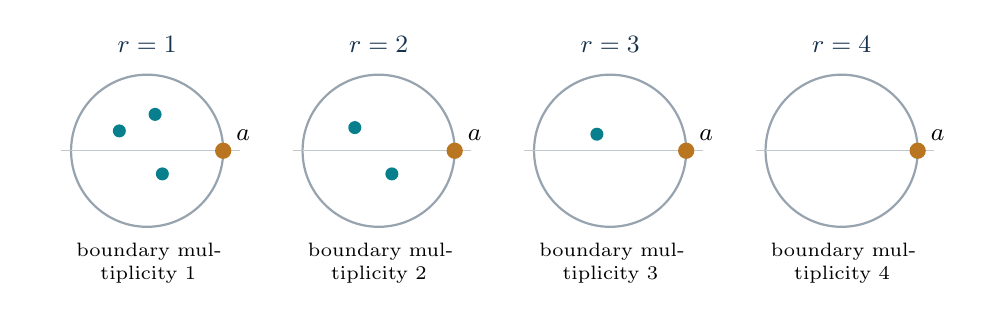
\begin{tikzpicture}[scale=.84]
\foreach \x/\r/\title in {0/1/{RH},3.5/2/{second moment level},7/3/{third moment level},10.5/4/{fourth moment level}} {
  \begin{scope}[shift={(\x,0)}]
  \draw[navy!45,thick] (0,0) circle(1.15);
  \draw[inkgray!35] (-1.3,0)--(1.4,0);
  \fill[gold] (1.15,0) circle(3.5pt);
  \node[anchor=west,font=\small] at (1.2,.23) {$a$};
  \node[font=\small\bfseries,navy] at (0,1.6) {$r=\r$};
  \node[font=\scriptsize,align=center,text width=2.8cm] at (0,-1.7) {boundary multiplicity \r};
  \end{scope}
}
\fill[teal] (-.42,.3) circle(2.8pt);
\fill[teal] (.12,.55) circle(2.8pt);
\fill[teal] (.23,-.35) circle(2.8pt);
\fill[teal] (3.14,.35) circle(2.8pt);
\fill[teal] (3.7,-.35) circle(2.8pt);
\fill[teal] (6.8,.25) circle(2.8pt);
\end{tikzpicture}
\caption{The possible multiplicities of the unique boundary root of
the degree-four limiting extremizer.  Gold marks the limiting direction;
teal marks the remaining interior roots.  This is a schematic of the
theorem, not a numerical plot of the prime polynomial.  Under the
stated fixed-strip input, RH is exactly the first case.}
\label{fc:base:rootpicture}
\end{figure}


% Consolidated source: Prime_Reciprocal_Circles_Further_Closures.tex, section-index 1
\section{The limiting extremal polynomial and its boundary multiplicity}
\label{fc:further:extremal}

The boundedness hierarchy for monic polynomial norms can be sharpened
to a theorem about the actual minimizing polynomials.  This gives an
exact location for the remaining obstruction inside a degree-four
polynomial whose norm is already bounded under the stated fixed-strip
input.  It also gives an explicit inverse bound for the original
deficit if that obstruction is removed.

We first state the result for a general sequence.  Let
\(u_n\to a\) with \(|u_n|=|a|=1\), let \(w_n>0\), and suppose
\(W_N=\sum_{n=2}^Nw_n\to\infty\).  Write
\[
 J_{k,N}=\sum_{n=2}^Nw_n|u_n-a|^{2k},\qquad
 J_{k,\infty}=\sum_{n\ge2}w_n|u_n-a|^{2k},
\]
and, for monic polynomials of degree \(m\), put
\[
 H_{m,N}=\min_{P(z)=z^m+\sum_{j<m}c_jz^j}
               \sum_{n=2}^Nw_n|P(u_n)|^2.
\]
Once at least \(m\) distinct sampled points have occurred, the
minimizer is unique; denote it by \(P_{m,N}\).

\begin{theorem}[Actual extremizer and exact boundary multiplicity]
\label{fc:further:limitpoly}
Assume that the set of sampled points is infinite and that
\(J_{m,\infty}<\infty\).  Define
\[
 r=\min\{k\in\{1,\ldots,m\}:J_{k,\infty}<\infty\},
 \qquad
 \nu_r=\sum_{n\ge2}w_n|u_n-a|^{2r}\delta_{u_n}.
\]
Then \(\nu_r\) is a finite positive measure with infinite support.
The polynomials \(P_{m,N}\) converge coefficient by coefficient to
the unique polynomial
\begin{equation}\label{fc:further:limitfactor}
 P_{m,\infty}(z)=(z-a)^r Q_{m-r}(z),
\end{equation}
where \(Q_{m-r}\) is the monic orthogonal polynomial of degree
\(m-r\) for \(\nu_r\); when \(m=r\), set \(Q_0=1\).
Moreover,
\begin{equation}\label{fc:further:limitnorm}
 H_{m,N}\uparrow H_{m,\infty}
 =\sum_{n\ge2}w_n|P_{m,\infty}(u_n)|^2
 =\min_{Q\ \mathrm{monic},\ \deg Q=m-r}
       \int |Q|^2\,d\nu_r>0.
\end{equation}
Every zero of \(Q_{m-r}\) lies strictly inside the unit disk.
Consequently \(a\) is the only zero of \(P_{m,\infty}\) on the unit
circle, and its multiplicity is exactly \(r\).
\end{theorem}

\begin{proof}
The minimum is nondecreasing in \(N\), and the trial polynomial
\((z-a)^m\) bounds it by \(J_{m,\infty}\).  Choose \(m\) distinct
sampled points at fixed indices.  Evaluation of the lower coefficients
at these points is an invertible Vandermonde map.  The bound on the
objective bounds the value of each minimizing polynomial at each of
these fixed points, and hence bounds all its lower coefficients.

Every subsequence therefore has a further coefficient-convergent
subsequence, with a monic degree-\(m\) limit \(P\).  If
\(H_{m,N}\uparrow H\), passage to the limit on each fixed finite
prefix gives
\[
 \sum_{n\ge2}w_n|P(u_n)|^2\le H.
\]
Conversely, for every monic degree-\(m\) polynomial \(R\) with
finite full energy, one has
\[
 H_{m,N}\le\sum_{n\le N}w_n|R(u_n)|^2,\qquad
 H\le\sum_{n\ge2}w_n|R(u_n)|^2.
\]
Thus every subsequential limit
is a minimizer of the full energy and its energy is exactly \(H\).

A nonzero polynomial \(R\) with \(R(a)\ne0\) has infinite energy,
because its modulus is bounded below on a tail while \(W_N\to\infty\).
More generally, if \(R(z)=(z-a)^s T(z)\) with \(T(a)\ne0\), its
energy is finite precisely when \(J_{s,\infty}<\infty\): on a tail
\(|T(u_n)|\) is bounded above and below by positive constants.
Since \(|u_n-a|\le2\), finite moments form an upper interval of
integer orders.  The monic degree-\(m\) polynomials of finite energy
are therefore exactly
\[
 (z-a)^r Q(z),\qquad Q\ \text{monic of degree }m-r.
\]
Their full energy is \(\int|Q|^2d\nu_r\).

Deleting the possible atom at \(a\) leaves infinitely many distinct
sampled points, so \(\nu_r\) has infinite support.  Its Gram matrix
on any fixed finite-dimensional polynomial space is positive definite:
a nonzero polynomial cannot vanish at infinitely many distinct points.
The preceding minimization consequently has a unique minimizer,
characterized by orthogonality to the lower-degree polynomials.  This
also makes its minimum strictly positive.  All subsequential limits
are this same polynomial, proving convergence of the entire sequence.

It remains to locate the zeros of \(Q=Q_{m-r}\).  If a zero
\(\xi\) satisfies \(|\xi|>1\), replacing the factor \(z-\xi\)
by \(z-1/\overline\xi\) gives another monic polynomial whose modulus
on the unit circle is smaller by the constant factor \(|\xi|\).
Its norm would be smaller, a contradiction.  If \(|\xi|=1\), write
\(Q(z)=(z-\xi)R(z)\).  Orthogonality to \(R\) gives
\[
 0=\int(z-\xi)|R(z)|^2\,d\nu_r(z).
\]
Thus \(\xi\) would be the average of unit vectors with positive
weights proportional to \(|R|^2d\nu_r\).  An average has unit
modulus only when all its mass is at that same unit vector; equivalently,
integrating \(|z-\xi|^2\) gives zero.  This is impossible for a
nonzero polynomial \(R\) and a measure with infinite support.
All the zeros are therefore strictly interior, in particular
\(Q(a)\ne0\).
\end{proof}

\begin{proposition}[Exact remaining-energy identity]
\label{fc:further:polysplitting}
Under the hypotheses of Theorem~\ref{fc:further:limitpoly}, for every
\(N\) at which the finite minimizer is unique,
\begin{align}
 H_{m,\infty}-H_{m,N}
 &=\sum_{n>N}w_n|P_{m,\infty}(u_n)|^2\notag\\
 &\quad+\sum_{n=2}^Nw_n
       |P_{m,\infty}(u_n)-P_{m,N}(u_n)|^2.
 \label{fc:further:polysplit}
\end{align}
Fix \(m\) distinct sampled points and let \(\lambda_0>0\) be the
smallest eigenvalue of their weighted Gram matrix on
\(1,z,\ldots,z^{m-1}\).  If \(c_{m,N}\) and \(c_{m,\infty}\)
are the vectors of lower coefficients, then, after these points have
occurred,
\begin{equation}\label{fc:further:coefficientbound}
 \|c_{m,N}-c_{m,\infty}\|_2^2
 \le\frac{H_{m,\infty}-H_{m,N}}{\lambda_0}.
\end{equation}
\end{proposition}

\begin{proof}
The difference between two monic degree-\(m\) polynomials has degree
at most \(m-1\).  Finite least-squares orthogonality therefore gives
\[
 \sum_{n\le N}w_n|P_{m,\infty}(u_n)|^2
 =H_{m,N}+\sum_{n\le N}w_n
       |P_{m,\infty}(u_n)-P_{m,N}(u_n)|^2.
\]
Add the tail and use \eqref{fc:further:limitnorm}.  Keeping the fixed
\(m\) points in the final sum bounds it below by \(\lambda_0\)
times the squared coefficient distance.
\end{proof}

The identity separates two quantities that a rate argument must
control: the tail of the limiting polynomial and the finite
projection error.  Smallness of the former alone does not bound
the latter.

\subsection{What a degree-four boundary root would settle}

Return to the original prime vectors and weights,
\[
 u_n=U_n=e^{2\pi i(S(p_n)-\log\log p_n)},\quad
 a=e^{2\pi i\BP},\quad w_n=p_{n+1}-p_{n-1}.
\]
Their support is infinite.  Indeed, finite support together with
\(U_n\to a\) would imply \(U_n=a\) eventually.  Since
\(E(p_n)\to0\), this would imply \(E(p_n)=0\) eventually, making
the sampled \(3/2\)-moment finite.  The sampling and integrability
spectrum in Theorem~\ref{fc:base:spectrum} exclude this: no
\(L^q\) energy with \(0<q<2\) is finite.

\begin{corollary}[A boundary multiplicity that encodes the zero strip]
\label{fc:further:primemultiplicity}
Whenever the prime \(2m\)-moment is finite, its limiting extremizer
has boundary multiplicity
\begin{equation}\label{fc:further:multtheta}
 r=\left\lceil\frac1{2(1-\Theta)}\right\rceil.
\end{equation}
In particular, using the separately supplied zero-free input
\(\Theta\le b_*<7/8\), the degree-four extremizers converge to a
well-defined polynomial \(P_{4,\infty}\).  Its only unit-circle
zero is \(a\), and the possibilities are exactly
\[
\begin{array}{c|c}
 \text{multiplicity of }a&\text{zero-boundary condition}\\ \hline
 1&\Theta=1/2\quad(\RH)\\
 2&1/2<\Theta\le3/4\\
 3&3/4<\Theta\le5/6\\
 4&5/6<\Theta\le b_*
\end{array}
\]
Consequently,
\begin{equation}\label{fc:further:simplerootcriterion}
 \RH\quad\Longleftrightarrow\quad
 P_{4,\infty}'(a)\ne0.
\end{equation}
The finite minimizing polynomials use no supplied value of \(\BP\);
the boundary point appears as a root of their limit.
\end{corollary}

\begin{proof}
The input spectrum states
\(J_{k,\infty}<\infty\) exactly when
\(\Theta\le1-1/(2k)\), including the endpoints.  The smallest
integer satisfying this condition is \eqref{fc:further:multtheta}.
Apply Theorem~\ref{fc:further:limitpoly}, and use that the functional
equation gives \(\Theta\ge1/2\).
\end{proof}

\begin{corollary}[Exact equality and strict improvement of the limit]
\label{fc:further:normgap}
Let \(C_{m,N}\) be the original normalized pair energy of order
\(2m\).  If \(J_{m,\infty}<\infty\), then
\[
 H_{m,\infty}=\lim_NC_{m,N}=J_{m,\infty}
 \quad\Longleftrightarrow\quad r=m.
\]
For \(r<m\), one has the strict inequality
\(H_{m,\infty}<\lim_NC_{m,N}\).
Thus under the stated fixed-strip input,
\begin{equation}\label{fc:further:fourthgap}
 H_{4,\infty}<\lim_NC_{4,N}
 \quad\Longleftrightarrow\quad \Theta\le5/6.
\end{equation}
\end{corollary}

\begin{proof}
The pair-energy limit is \(J_{m,\infty}\).  If \(r=m\), the
only admissible monic polynomial of finite energy is \((z-a)^m\).
If \(r<m\), the trial quotient \((z-a)^{m-r}\) has a boundary
zero and therefore differs from the unique minimizing quotient,
whose zeros are all strictly interior.  Positive definiteness of the
finite-measure Gram matrix makes the inequality of their squared
norms strict.
\end{proof}

A finite positive difference between the two diagnostics is not
by itself a certificate for \eqref{fc:further:fourthgap}: that statement
compares their infinite limits.  The projection term in
\eqref{fc:further:polysplit} is among the quantities that must be
controlled to turn it into a certified finite computation.

\subsection{An inverse bound for the original deficit}

\begin{proposition}[Interior-root gaps control the original budget]
\label{fc:further:inversebound}
In Theorem~\ref{fc:further:limitpoly}, suppose \(r=1\), and write
\[
 P_{m,\infty}(z)=(z-a)\prod_{j=1}^{m-1}(z-\xi_j),\qquad
 g=\prod_{j=1}^{m-1}(1-|\xi_j|)>0.
\]
Empty products equal one.  For the original deficit
\(D_N=W_N-|\sum_{n\le N}w_nu_n|\), one has
\begin{equation}\label{fc:further:rootgapbound}
 \sup_N D_N=D_\infty=\frac{J_{1,\infty}}2
 \le \frac{H_{m,\infty}}{2g^2}.
\end{equation}

There is also a bound using the boundary derivative and a finite
prefix.  Suppose \(m\ge2\), put
\(d=|P_{m,\infty}'(a)|>0\) and \(s=m-1\), and choose \(L\)
so that
\[
 |u_n-a|\le\frac{d}{s2^s}\qquad(n>L).
\]
Then
\begin{equation}\label{fc:further:derivativebound}
 D_\infty\le\frac{J_{1,L}}2+\frac{2H_{m,\infty}}{d^2}
 \le2W_L+\frac{2H_{m,\infty}}{d^2}.
\end{equation}
For degree four the required tail radius is \(d/24\).
\end{proposition}

\begin{proof}
For \(|z|=1\), the reverse triangle inequality gives
\(|\prod(z-\xi_j)|\ge g\).  Hence
\(H_{m,\infty}\ge g^2J_{1,\infty}\).
The usual variance identity, or the limiting pair-energy identity
at order two, gives \(V_N\to J_{1,\infty}\).  Since
\(V_N=D_N(1+|\sum w_nu_n|/W_N)\) and the normalized resultant
tends to \(a\), it follows that
\(D_N\to J_{1,\infty}/2\).  The triangle inequality makes
\(D_N\) nondecreasing, which proves \eqref{fc:further:rootgapbound}.

Let \(Q(z)=\prod_{j=1}^s(z-\xi_j)\).  On the closed unit disk,
\(|Q'(z)|\le s2^{s-1}\).  The line segment joining \(a\) and
any \(u_n\) lies in that disk, so
\[
 |Q(u_n)-Q(a)|\le s2^{s-1}|u_n-a|.
\]
Because \(|Q(a)|=d\), the stated tail radius ensures
\(|Q(u_n)|\ge d/2\) for \(n>L\).  Therefore
\[
 \sum_{n>L}w_n|u_n-a|^2
 \le\frac4{d^2}\sum_{n>L}w_n|P_{m,\infty}(u_n)|^2
 \le\frac{4H_{m,\infty}}{d^2}.
\]
Add the prefix and divide by two; finally use
\(J_{1,L}\le4W_L\).
\end{proof}

The simple-root condition, or a positive lower bound for its
derivative, is the remaining arithmetic assertion.  Positivity of
the finite Gram matrices proves neither.  The inverse bounds show
precisely how such an assertion would supply the original uniform
constant, without changing the weights or replacing the objective
by a higher moment.

\begin{proposition}[A finite radial-gap certificate without centering]
\label{fc:further:finitegap}
For a finite positive weighted unit-circle configuration, let
\(P_{m,N}(z)=\prod_{j=1}^m(z-\xi_{j,N})\) be its monic minimizing
polynomial, and put
\(M_N=\sum_{n\le N}w_nu_n\) and \(m_N=M_N/W_N\).
Choose one root \(\xi_{1,N}\).  If the other roots satisfy
\(|\xi_{j,N}|<1\), define
\[
 g_N=\prod_{j=2}^m(1-|\xi_{j,N}|)>0.
\]
Then the original variance and deficit satisfy
\begin{equation}\label{fc:further:finitegapbound}
 V_N\le\frac{H_{m,N}}{g_N^2},\qquad
 D_N\le\frac{H_{m,N}}{g_N^2(1+|m_N|)}.
\end{equation}
In particular, if those \(m-1\) roots lie in
\(|z|\le1-\eta\), then
\[
 D_N\le\frac{H_{m,N}}{\eta^{2m-2}(1+|m_N|)}.
\]
Every term in these finite bounds is obtained from the original
vectors and weights; no limiting direction or centering constant
is supplied.
\end{proposition}

\begin{proof}
For \(|u_n|=1\), factorization and the reverse triangle inequality
give
\[
 |P_{m,N}(u_n)|^2
 \ge g_N^2|u_n-\xi_{1,N}|^2.
\]
The weighted variance minimizes the last squared-distance sum over
all complex centers, so
\[
 H_{m,N}\ge g_N^2\sum_{n\le N}w_n|u_n-\xi_{1,N}|^2
 \ge g_N^2 V_N.
\]
Finally \(V_N=D_N(1+|m_N|)\).
\end{proof}

\begin{corollary}[The second largest root is the remaining condition]
\label{fc:further:secondroot}
For the original prime sequence, use the stated fixed-strip input
that bounds \(H_{4,N}\).  Order the moduli of the four roots of
\(P_{4,N}\) as
\(\rho_{1,N}\ge\rho_{2,N}\ge\rho_{3,N}\ge\rho_{4,N}\).
Then
\begin{equation}\label{fc:further:secondrootcriterion}
 \RH\quad\Longleftrightarrow\quad
 \limsup_{N\to\infty}\rho_{2,N}<1.
\end{equation}
More concretely, if \(H_{4,N}\le B\) and
\(\rho_{2,N}\le1-\eta\) for all sufficiently large \(N\), then
\begin{equation}\label{fc:further:finitegapK}
 \sup_ND_N\le\frac{B}{2\eta^6}.
\end{equation}
\end{corollary}

\begin{proof}
Coefficient convergence of monic polynomials implies convergence
of their multisets of roots, including multiplicities, and hence of
their ordered root moduli.  By
Corollary~\ref{fc:further:primemultiplicity}, under RH exactly one
limiting root is on the unit circle; without RH at least two are.
This proves \eqref{fc:further:secondrootcriterion}.

Alternatively the sufficient implication follows immediately from
Proposition~\ref{fc:further:finitegap}, the bound on \(H_{4,N}\), and
the original deficit criterion.  For its explicit constant, use
\(|m_N|\to1\) in the finite bound and take the limit.  Monotonicity
of \(D_N\) makes its limit its supremum, so the eventual root-gap
bound also controls every earlier prefix.
\end{proof}

\begin{proposition}[A fourfold boundary limit with divergent deficit]
\label{fc:further:fourfoldexample}
Consider the independent sequence
\[
 w_n=1,\qquad u_n=\exp(i n^{-1/7})\quad(n\ge1),\qquad
 \mathcal D_N=N-\left|\sum_{n=1}^N u_n\right|.
\]
Its fourth extremal norms are bounded, but their limiting polynomial is
\[
 P_{4,\infty}(z)=(z-1)^4,
\]
and
\begin{equation}\label{fc:further:exampleasymptotic}
 \mathcal D_N=\frac7{360}N^{5/7}+O(N^{3/7}).
\end{equation}
Thus a uniform bound for the fourth extremal norm, positivity of the
finite Gram matrices, and convergence of the phase vectors do not
alone force a simple boundary root.
\end{proposition}

\begin{proof}
The support is infinite and \(u_n\to1\).  Since
\(|u_n-1|\sim n^{-1/7}\), the moment
\(\sum_n|u_n-1|^{2k}\) is finite precisely when \(2k>7\).
Its smallest finite integer order is therefore \(r=4\), so
Theorem~\ref{fc:further:limitpoly} gives the asserted limiting polynomial.

Elementary sums of powers and the Taylor remainders for sine and cosine
give
\begin{align*}
 \Re\sum_{n=1}^Nu_n
   &=N-\frac7{10}N^{5/7}+O(N^{3/7}),\\
 \Im\sum_{n=1}^Nu_n
   &=\frac76N^{6/7}+O(N^{4/7}).
\end{align*}
Squaring and taking the square root yields
\[
 \left|\sum_{n=1}^Nu_n\right|
 =N+\frac12\left(-\frac75+\frac{49}{36}\right)N^{5/7}
      +O(N^{3/7})
 =N-\frac7{360}N^{5/7}+O(N^{3/7}).
\]
This proves \eqref{fc:further:exampleasymptotic}.
\end{proof}

This example is not the prime construction and is not a counterexample
to RH.  It isolates the additional arithmetic content required by the
radial-gap criterion: in this example all four extremal roots approach
the boundary point, so the required uniform gap fails.

\subsection{A quantitative fourth-pair-energy rate under $(H_b)$}

The pair energy has a rate that follows directly from a strict
fixed-strip input; it does not require the simple-root condition.

\begin{proposition}[Rate from a fixed strip]
\label{fc:further:pairrate}
Suppose the original prime sequence satisfies
\[
 |U_n-a|\ll \frac{p_n^{-\eta}}{\log p_n},\qquad
 \frac18<\eta<\frac17.
\]
Then, with \(X=p_N\) and \(\delta=8\eta-1>0\),
\begin{equation}\label{fc:further:C4rate}
 C_{4,N}=J_{4,\infty}
   +O\!\left(\frac{X^{-\delta}}{(\log X)^8}\right).
\end{equation}
In particular the separately supplied bound
\(E(x)=O(x^{b_*-1}/\log x)\) gives
\begin{align*}
 b_*&=0.87495701942009894612860385056145\ldots,\\
 \delta&=7-8b_*
 =0.0003438446392084309711691955084\ldots.
\end{align*}
The implicit constants include those in the analytic fixed-strip
estimate; no certified numerical error bar follows without them.
\end{proposition}

\begin{proof}
Put \(d_n=U_n-a\) and
\(S_{r,s,N}=\sum_{n\le N}w_nd_n^r\overline{d_n}^{\,s}\), with
\(S_{0,0,N}=W_N\).  Expanding the two fourth powers gives the exact
finite identity
\begin{equation}\label{fc:further:C4expansion}
 C_{4,N}=\frac1{2W_N}
 \sum_{r,s=0}^4(-1)^{r+s}\binom4r\binom4s
             S_{4-r,4-s,N}S_{r,s,N}.
\end{equation}
The terms \((r,s)=(0,0),(4,4)\) sum to \(J_{4,N}\).
For every other term the two total orders are integers
\(\ell\) and \(8-\ell\), with \(1\le\ell\le7\).

Bertrand's postulate bounds neighboring prime ratios.  Comparison
over the adjacent prime gaps, whose overlap is at most two, gives
for \(1\le\ell\le7\)
\[
 \sum_{n\le N}w_n|d_n|^\ell
 \ll 1+\int_3^{2X}\frac{x^{-\ell\eta}}{(\log x)^\ell}\,dx
 \ll\frac{X^{1-\ell\eta}}{(\log X)^\ell}.
\]
Here \(\ell\eta<1\), and \(W_N\asymp X\).  Every non-endpoint
term in \eqref{fc:further:C4expansion} is consequently
\(O(X^{1-8\eta}/(\log X)^8)\).  The same gap comparison on the
tail gives
\[
 J_{4,\infty}-J_{4,N}
 \ll\int_X^\infty\frac{x^{-8\eta}}{(\log x)^8}\,dx
 \ll\frac{X^{1-8\eta}}{(\log X)^8}.
\]
Combining these estimates proves the proposition.
\end{proof}

At the weaker boundary value \(\eta=1/8\), the same proof instead
gives \(C_{4,N}=J_{4,\infty}+O((\log X)^{-7})\): the non-endpoint
terms are \(O((\log X)^{-8})\), while the tail integral is of
order \((\log X)^{-7}\).  Neither rate is a bound for the
degree-one deficit.  The limiting-polynomial criterion above states
the additional condition that would yield that bound.


% Consolidated source: Prime_Reciprocal_Circles_Further_Closures.tex, section-index 2
\section{The exactly centered Laguerre endpoint and Li's chart}
\label{fc:li:section}

The Laguerre scale \(\alpha=1/2\) places the expansion center at
\(s=1\) and makes the disk coordinate exactly Li's coordinate.
This endpoint is admissible for the exactly centered prime error.
Its justification requires both absolute convergence of the individual
coefficients and a genuine holomorphic germ at \(s=1\).
We retain
\[
 E(x)=\sum_{p\le x}\frac1p-\log\log x-\BP,
 \qquad F(s)=\int_2^\infty E(x)x^{-s}\dd x\quad(\Re s>1),
\]
and use the ordinary Laguerre polynomials
\[
 L_n(t)=\sum_{j=0}^n(-1)^j\binom nj\frac{t^j}{j!}.
\]

\begin{lemma}[Absolute endpoint moments and a holomorphic germ]
\label{fc:li:germ}
For every nonnegative integer \(j\),
\[
 \int_2^\infty |E(x)|x^{-1}(\log x)^j\dd x<\infty.
\]
The initially defined function \(F\) extends holomorphically across
\(s=1\), and its derivatives there are
\begin{equation}\label{fc:li:derivatives}
 F^{(j)}(1)=\int_2^\infty E(x)x^{-1}(-\log x)^j\dd x.
\end{equation}
\end{lemma}

\begin{proof}
Write \(\Delta(x)=\pi(x)-\operatorname{li}(x)\).
The unconditional estimate of Johnston and Yang
\cite[Corollary~1.3]{fc:li-johnstonyang} gives
\[
 |\Delta(x)|\le 9.59x(\log x)^{0.515}
           e^{-0.8274\sqrt{\log x}}\qquad(x\ge2).
\]
Partial summation, with the constant fixed by \(E(x)\to0\), yields
\[
 E(x)=\frac{\Delta(x)}x-\int_x^\infty\frac{\Delta(y)}{y^2}\dd y.
\]
After decreasing the positive exponential constant, this implies
\begin{equation}\label{fc:li:pntdecay}
 E(e^t)=O(e^{-c_0\sqrt t})\qquad(t\to\infty)
\end{equation}
for some \(c_0>0\).  It proves the asserted absolute moments.

To establish holomorphic continuation, define
\begin{equation}\label{fc:li:primepower}
 P(s)=\sum_p p^{-s}\quad(\Re s>1),\qquad
 R_0(s)=\sum_{k\ge2}\frac{P(ks)}k.
\end{equation}
\begin{equation}\label{fc:li:jzero}
 \begin{split}
 c&=\log\log2+\BP,\\
 J_0(s)&=c\,2^{1-s}-\gamma-\log\log2
       -\sum_{j\ge1}\frac{[-(s-1)\log2]^j}{j\,j!}.
 \end{split}
\end{equation}
The series for \(R_0\) converges normally on \(\Re s>1/2\),
and \(J_0\) is entire.  For \(\Re s>1\), integration of the
prime sum and of \(\log\log x\) gives
\[
 (s-1)F(s)=P(s)-c\,2^{1-s}
                -\int_2^\infty\frac{x^{-s}}{\log x}\dd x.
\]
Using the Euler product and the exponential-integral expansion gives
\begin{equation}\label{fc:li:mellinidentity}
 F(s)=\frac{\log((s-1)\zeta(s))-R_0(s)-J_0(s)}{s-1}.
\end{equation}
The logarithm is initially the branch agreeing with real values for
real \(s>1\).

The function \(H(s)=(s-1)\zeta(s)\) is holomorphic near \(1\),
with \(H(1)=1\), so \(\log H\) has a holomorphic branch there
with value zero at \(1\).  The exact constant identity
\(\BP=\gamma-R_0(1)\) gives
\(J_0(1)=\BP-\gamma=-R_0(1)\).
The numerator of \eqref{fc:li:mellinidentity} therefore vanishes at
\(1\), making its apparent pole removable.
Finally, differentiate the integral at real \(\sigma>1\) and let
\(\sigma\downarrow1\).  The absolute moments already proved give
dominated convergence, and continuity of the holomorphic derivatives
gives \eqref{fc:li:derivatives}.
\end{proof}

\begin{remark}\label{fc:li:germcaution}
The decay \eqref{fc:li:pntdecay} alone supplies all one-sided derivatives
at the original boundary; it does not by itself supply a holomorphic
extension.  Formula \eqref{fc:li:mellinidentity} is the additional step
that makes the endpoint argument valid.
\end{remark}

\begin{theorem}[The endpoint Laguerre criterion]
\label{fc:li:endpoint}
The numbers
\begin{equation}\label{fc:li:bn}
 b_n=\int_2^\infty E(x)x^{-1}L_n(\log x)\dd x,
 \qquad n\ge0,
\end{equation}
are unconditionally absolutely convergent.  The holomorphic germ
\begin{equation}\label{fc:li:gstar}
 G_*(z)=\frac1{1-z}F\!\left(\frac1{1-z}\right)
\end{equation}
has Taylor coefficients \(b_n\).  Moreover,
\begin{equation}\label{fc:li:equivalence}
 \RH\quad\Longleftrightarrow\quad (b_n)_{n\ge0}\in\ell^2
 \quad\Longleftrightarrow\quad
 G_*\text{ extends to }H^2(\mathbb D).
\end{equation}
When these conditions hold,
\begin{equation}\label{fc:li:normidentity}
 \sum_{n\ge0}|b_n|^2
 =\|G_*\|_{H^2}^2
 =\int_2^\infty E(x)^2\dd x.
\end{equation}
The Hardy norm uses normalized angular measure on the unit circle.
\end{theorem}

\begin{proof}
Absolute convergence follows from Lemma~\ref{fc:li:germ} and the
finite degree of \(L_n\).  Expanding that polynomial gives
\begin{equation}\label{fc:li:triangular}
 b_n=\sum_{j=0}^n\binom nj\frac{F^{(j)}(1)}{j!}.
\end{equation}
Since \(F\) is an actual holomorphic germ at \(1\), ordinary Taylor
algebra applied to \(s-1=z/(1-z)\) shows that the coefficient of
\(z^n\) in \eqref{fc:li:gstar} is exactly \eqref{fc:li:triangular}.
No exchange of an infinite Laguerre series with the endpoint integral
is needed.

Put
\[
 f(t)=e^{t/2}E(e^t)\mathbf1_{\{t\ge\log2\}},\qquad
 \ell_n(t)=e^{-t/2}L_n(t),\qquad t\ge0.
\]
The functions \(\ell_n\) are orthonormal in \(L^2(0,\infty)\)
by the Laguerre orthogonality relation \cite[Table~18.3.1]{fc:li-dlmf}.
For completeness, if \(h\in L^2(0,\infty)\) is orthogonal to all
\(\ell_n\), triangularity of the polynomials makes every derivative
of \(\mathcal Lh(w)=\int_0^\infty h(t)e^{-wt}\dd t\) vanish at
\(w=1/2\).  This Laplace transform is holomorphic on \(\Re w>0\),
so the identity theorem and Laplace uniqueness give \(h=0\).
Thus the system is an orthonormal basis.  Also
\(b_n=\int_0^\infty f(t)\ell_n(t)\dd t\), and
\[
 \int_0^\infty |f(t)|^2\dd t=\int_2^\infty E(x)^2\dd x.
\]
Theorem~\ref{fc:base:energy} and Parseval prove the forward implication
and the norm identity.

Conversely, suppose \((b_n)\in\ell^2\).  The orthonormal basis
produces \(h\in L^2(0,\infty)\) with precisely those coefficients.
For \(g=f-h\), polynomial triangularity gives
\begin{equation}\label{fc:li:zeromoments}
 \int_0^\infty g(t)e^{-t/2}t^j\dd t=0\qquad(j\ge0).
\end{equation}
All these integrals converge absolutely, by \eqref{fc:li:pntdecay}
for \(f\) and by Cauchy--Schwarz for \(h\).
Initially on \(\Re w>1/2\),
\[
 \mathcal Lg(w)=F(w+1/2)-\mathcal Lh(w).
\]
Lemma~\ref{fc:li:germ} and the holomorphy of \(\mathcal Lh\) on
\(\Re w>0\) extend this difference across \(w=1/2\).
Its derivatives at that point are zero by \eqref{fc:li:zeromoments},
where the derivative identities follow by the same dominated limits
as in Lemma~\ref{fc:li:germ}.  The identity theorem first makes the
difference zero locally, and then on \(\Re w>1/2\).
For any real \(\sigma>1/2\), the function \(e^{-\sigma t}g(t)\)
is in \(L^1(0,\infty)\), and its Fourier transform is zero.
Fourier uniqueness gives \(g=0\) almost everywhere.
Consequently \(f=h\in L^2\), and Theorem~\ref{fc:base:energy} gives
\(\RH\).  Finally, the usual coefficient characterization of
\(H^2(\mathbb D)\) proves the other equivalence and its norm equality.
\end{proof}

\subsection{An explicit corrected-Li square-summability condition}

Use the conventional completed zeta function and Li coefficients
\cite[\S1]{fc:li-lagarias}:
\begin{align}
 \xi(s)&=\tfrac12s(s-1)\pi^{-s/2}\Gamma(s/2)\zeta(s),
 \qquad \xi(1)=\tfrac12,\label{fc:li:xi}\\
 \lambda_n&=\frac1{(n-1)!}
 \left.\frac{\mathrm d^n}{\mathrm d s^n}
 \{s^{n-1}\log\xi(s)\}\right|_{s=1},\qquad n\ge1.
 \label{fc:li:lambda}
\end{align}
Set
\begin{align}
 s(z)&=\frac1{1-z},\qquad
 A(s)=-\log s+\frac{s}{2}\log\pi-\log\Gamma(s/2),
 \label{fc:li:arch}\\
 C(z)&=A(s(z))-R_0(s(z))-J_0(s(z)),
 \qquad c_n=[z^n]C(z).\label{fc:li:correction}
\end{align}
The logarithms in \(A\) are the holomorphic branches on
\(\Re s>1/2\) that are real on the positive real axis.
In particular, \(A(1)=0\).

\begin{proposition}[Exact bridge to Li's coefficients]
\label{fc:li:bridge}
The function \(C\) is holomorphic throughout \(\mathbb D\),
unconditionally, and \(C(0)=0\).  The following identities hold as
holomorphic germs at \(z=0\):
\begin{align}
 zG_*(z)&=\log\bigl(2\xi(s(z))\bigr)+C(z),
 \label{fc:li:bridgegerm}\\
 b_{n-1}&=\frac{\lambda_n}{n}+c_n\qquad(n\ge1).
 \label{fc:li:bridgecoeff}
\end{align}
Consequently,
\begin{equation}\label{fc:li:correctedcriterion}
 \RH\quad\Longleftrightarrow\quad
 \sum_{n\ge1}\left|\frac{\lambda_n}{n}+c_n\right|^2<\infty.
\end{equation}
If finite, this sum is exactly \(\int_2^\infty E(x)^2\dd x\).
\end{proposition}

\begin{proof}
The map \(s(z)\) sends \(\mathbb D\) into \(\Re s>1/2\).
The asserted holomorphy therefore follows from the definitions of
\(A,R_0,J_0\); their values at \(1\) give \(C(0)=0\).
Near \(s=1\), the definition of \(\xi\) gives
\[
 \log((s-1)\zeta(s))=\log(2\xi(s))+A(s).
\]
Insert this into \eqref{fc:li:mellinidentity} and use
\(s(z)-1=z/(1-z)\) to obtain \eqref{fc:li:bridgegerm}.
If \(\Phi(s)=\log(2\xi(s))\), finite Taylor algebra and the
Leibniz rule in \eqref{fc:li:lambda} give, for \(n\ge1\),
\[
 [z^n]\Phi(s(z))
 =\sum_{j=1}^n\binom{n-1}{j-1}\frac{\Phi^{(j)}(1)}{j!}
 =\frac{\lambda_n}{n}.
\]
This proves \eqref{fc:li:bridgecoeff}; Theorem~\ref{fc:li:endpoint}
then proves \eqref{fc:li:correctedcriterion} and the norm assertion.
\end{proof}

\begin{corollary}[The prime-power endpoint has no prime-zeta correction]
\label{fc:li:primepowerbridge}
Define
\[
 E^{\mathrm{pp}}(x)=
 \sum_{p^k\le x}\frac1{kp^k}-\log\log x-\gamma,\qquad
 b_n^{\mathrm{pp}}=\int_2^\infty
             E^{\mathrm{pp}}(x)x^{-1}L_n(\log x)\dd x,
\]
and put \(J_{\mathrm{pp}}(s)=J_0(s)+(\gamma-\BP)2^{1-s}\).
All these endpoint coefficients converge absolutely, and
\begin{equation}\label{fc:li:primepowercoeff}
 b_{n-1}^{\mathrm{pp}}
 =\frac{\lambda_n}{n}
   +[z^n]\{A(s(z))-J_{\mathrm{pp}}(s(z))\}\qquad(n\ge1).
\end{equation}
Moreover, \((b_n^{\mathrm{pp}})\in\ell^2\) if and only if \(\RH\);
when finite, its squared norm is
\(\int_2^\infty |E^{\mathrm{pp}}(x)|^2\dd x\).
\end{corollary}

\begin{proof}
The bias is
\[
 E(x)-E^{\mathrm{pp}}(x)
 =\sum_{\substack{k\ge2\\p^k>x}}\frac1{kp^k}
 =O\!\left(\frac1{\sqrt x\log x}\right).
\]
For \(k=2\), this bound follows by partial summation from
\(\pi(y)\ll y/\log y\); splitting \(k\ge3\) at
\(\lfloor\log x/\log2\rfloor\) gives
\(O(x^{-2/3}\log x)\) for the remaining terms.
The bias is therefore in \(L^2(2,\infty)\) and has every endpoint
logarithmic moment.  Initially for \(\Re s>1\), the Euler product gives
\[
 F^{\mathrm{pp}}(s):=\int_2^\infty E^{\mathrm{pp}}(x)x^{-s}\dd x
 =\frac{\log((s-1)\zeta(s))-J_{\mathrm{pp}}(s)}{s-1}.
\]
Since \(J_{\mathrm{pp}}(1)=0\), its singularity at \(1\) is
removable.  The proof of Theorem~\ref{fc:li:endpoint} now applies
unchanged, and the \(L^2\) bias transfers the RH equivalence.
The identity with \(\xi\) gives \eqref{fc:li:primepowercoeff}.
\end{proof}

\begin{corollary}[The endpoint radius and its singularities]
\label{fc:li:radius}
The Taylor radius of \(G_*\) is
\begin{equation}\label{fc:li:radiusformula}
 R_*=
 \min\left\{1,\inf_{\substack{\zeta(\rho)=0\\\Re\rho>1/2}}
                 \left|1-\frac1\rho\right|\right\},
\end{equation}
where the infimum of the empty set is \(+\infty\).
Thus \(R_*=1\) if and only if \(\RH\); equivalently,
\(\limsup_{n\to\infty}|b_n|^{1/n}=1\) if and only if \(\RH\).
\end{corollary}

\begin{proof}
Within \(\Re s>1/2\), the only possible obstructions in
\eqref{fc:li:mellinidentity}, apart from the already removed point \(1\),
are zeros of \(\zeta\).  At a zero \(\rho\) of multiplicity
\(m_\rho\), on a slit neighborhood,
\[
 F(s)=\frac{m_\rho}{s-1}\log(s-\rho)+H_\rho(s),
\]
where \(H_\rho\) is holomorphic.  Since
\(z_\rho=1-1/\rho\ne0\) and the change of variable has nonzero
derivative there, \(G_*\) has a nonremovable logarithmic branch
at \(z_\rho\).  A disk about zero containing no such image admits
the normalized holomorphic logarithm in \eqref{fc:li:mellinidentity}.

There is also an unconditional boundary obstruction at \(z=-1\).
For real \(s=1/2+\varepsilon\),
\[
 R_0(s)=-\tfrac12\log\varepsilon+O(1),\qquad
 F(s)=-\log\varepsilon+O(1)
 \quad(\varepsilon\downarrow0).
\]
The first relation comes from the term \(P(2s)/2\); all terms
with \(k\ge3\) remain bounded.  The other terms in the numerator
of \eqref{fc:li:mellinidentity} are regular on this real approach.
Hence \(G_*(z)=-\tfrac12\log(1+z)+O(1)\) as real
\(z\downarrow-1\) from within the disk, preventing a radius
larger than one.  This proves \eqref{fc:li:radiusformula}.
Finally, \(|1-1/\rho|<1\) exactly when \(\Re\rho>1/2\),
and the functional equation supplies such a zero whenever RH fails.
Cauchy--Hadamard gives the coefficient statement.
\end{proof}

\begin{remark}[Exact centering is essential at this endpoint]
\label{fc:li:centering}
If \(E\) is replaced by \(E_\delta=E-\delta\) with
\(\delta\ne0\), every integral in \eqref{fc:li:bn} fails to converge:
the added term is the integral of a nonzero constant times the
polynomial \(L_n(t)\) over an infinite interval.  Analytically,
\[
 F_\delta(s)=F(s)-\delta\frac{2^{1-s}}{s-1},\qquad
 G_{*,\delta}(z)=G_*(z)-\frac{\delta}{z}
                         2^{\,1-1/(1-z)}.
\]
Thus the miscentered expression has a simple pole at the expansion
center, with residue \(-\delta\).  The endpoint bridge uses the
exact constant \(\BP\); it does not turn an approximate centering
constant into valid endpoint coefficients.  The corrected-Li
criterion is a proved equivalence, not an estimate of its infinite sum.
\end{remark}


% Consolidated source: Prime_Reciprocal_Circles_Further_Closures.tex, section-index 3
\section{Exact spectral mass limits for the circle measures}
\label{fc:sp:section}

The normalized Toeplitz matrices converge to rank one.  The following
results identify exactly what remains after multiplication by the
diverging total mass.  They apply to arbitrary converging unit phases,
including finite-support examples, and specialize to the prime phases
\(u_n=U_n\), weights \(w_n\), and limit \(a=u_\infty\).

Fix \(r\ge1\) and write \(L=r+1\).  Throughout this section assume
\begin{equation}\label{fc:sp:assumptions}
 |u_n|=|a|=1,\qquad u_n\longrightarrow a,\qquad
 w_n>0,\qquad W_N=\sum_{n=2}^Nw_n\longrightarrow\infty.
\end{equation}
Define
\begin{align}
 v(u)&=(1,u,\ldots,u^r)^{\mathsf T},\qquad
 e=\frac{v(a)}{\sqrt L},\qquad \Pi=I-ee^*,\label{fc:sp:features}\\
 A_N&=\sum_{n=2}^Nw_nv(u_n)v(u_n)^*,\qquad
 T_{r,N}=\frac{A_N}{W_N},\label{fc:sp:matrices}\\
 m_{k,N}&=\frac1{W_N}\sum_{n=2}^Nw_nu_n^k,
 \qquad V_N^{(k)}=W_N(1-|m_{k,N}|^2).\label{fc:sp:harmonics}
\end{align}
Thus \((T_{r,N})_{jk}=m_{j-k,N}\) for \(0\le j,k\le r\).
Let \(\ell_{1,N}\ge\cdots\ge\ell_{L,N}\ge0\) be the
eigenvalues of \(A_N\), and put
\begin{align}
 \mathcal L_{r,N}&=LW_N-\ell_{1,N}
                  =\sum_{j=2}^L\ell_{j,N},\label{fc:sp:leakage}\\
 \mathcal T_{r,N}&=W_Ne_2(T_{r,N}),\qquad
 e_2(T)=\sum_{i<j}\lambda_i(T)\lambda_j(T).
 \label{fc:sp:secondminor}
\end{align}

\begin{theorem}[Monotone leakage and its exact limiting energy]
\label{fc:sp:masslimit}
Under \eqref{fc:sp:assumptions}, \(\mathcal L_{r,N}\) is
nondecreasing, and
\begin{align}
 \mathcal L_{r,\infty}
 :=\lim_{N\to\infty}\mathcal L_{r,N}
 &=\sum_{n=2}^\infty w_n\|\Pi v(u_n)\|^2\label{fc:sp:limitprojection}\\
 &=\frac1L\sum_{n=2}^\infty w_n
             \sum_{k=1}^r(L-k)|u_n^k-a^k|^2.\label{fc:sp:limitchords}
\end{align}
The equalities hold in \([0,\infty]\); no summability assumption
is needed.  In particular, this limit is finite exactly when
\(\sum_nw_n|u_n-a|^2<\infty\).  For the prime phases and weights,
its finiteness is equivalent to \(\RH\).
\end{theorem}

\begin{proof}
The Rayleigh principle gives the exact finite-dimensional identity
\begin{equation}\label{fc:sp:variational}
 \mathcal L_{r,N}
 =\min_{\|b\|=1} Q_N(b),\qquad
 Q_N(b)=\sum_{n=2}^Nw_n\{L-|b^*v(u_n)|^2\}.
\end{equation}
Each summand is nonnegative by Cauchy--Schwarz, since
\(\|v(u_n)\|^2=L\).  Hence \(Q_N\) increases pointwise with
\(N\), and its minima are nondecreasing.

Suppose first that their limit \(q\) is finite.  Choose a minimizer
\(b_N\) on the compact unit sphere and take a convergent subsequence
\(b_N\to b_*\).  For each fixed \(M\),
\(Q_M(b_N)\le\mathcal L_{r,N}\) when \(N\ge M\).
Continuity and then monotone convergence give
\(Q_\infty(b_*)\le q\).
If \(L-|b_*^*v(a)|^2\) were positive, convergence \(u_n\to a\)
would give a positive lower bound on that factor on a tail, and
\(W_N\to\infty\) would force \(Q_\infty(b_*)=\infty\).
Equality in Cauchy--Schwarz therefore implies that \(b_*\) is a
unit scalar multiple of \(e\).  Thus \(Q_\infty(e)\le q\).
Conversely, testing \(b=e\) in \eqref{fc:sp:variational} gives
\(\mathcal L_{r,N}\le Q_N(e)\), so \(q=Q_\infty(e)\).
If \(q=\infty\), the same test shows that \(Q_\infty(e)\)
cannot be finite.  This proves \eqref{fc:sp:limitprojection} in both
cases.

For \(u\in\mathbb T\), expand the squared geometric sum to obtain
\[
 \|\Pi v(u)\|^2
 =L-\frac1L\left|\sum_{j=0}^r(u\overline a)^j\right|^2
 =\frac1L\sum_{k=1}^r(L-k)|u^k-a^k|^2.
\]
This gives \eqref{fc:sp:limitchords}.  Its \(k=1\) term gives the
lower bound \(r|u-a|^2/L\), while
\(|u^k-a^k|\le k|u-a|\) gives a fixed multiple of
\(|u-a|^2\) as an upper bound.  The finiteness equivalence follows.
The specialization to primes uses Theorem~\ref{fc:base:energy}.
\end{proof}

\begin{corollary}[The original deficit is the first spectral case]
\label{fc:sp:firstcase}
Let \(D_N=W_N-|\sum_{n=2}^Nw_nu_n|\).  Then
\(\mathcal L_{1,N}=D_N\), and
\begin{equation}\label{fc:sp:deficitlimit}
 \lim_{N\to\infty}D_N
 =\frac12\sum_{n=2}^\infty w_n|u_n-a|^2
 \quad\text{in }[0,\infty].
\end{equation}
For every fixed \(r\), if these limits are finite, then
\begin{equation}\label{fc:sp:limitcomparison}
 \frac{2r}{r+1}D_\infty
 \le\mathcal L_{r,\infty}
 \le\binom{r+2}{3}D_\infty.
\end{equation}
\end{corollary}

\begin{proof}
For \(r=1\), the eigenvalues of \(T_{1,N}\) are
\(1\pm|m_{1,N}|\), proving the first assertion and then
\eqref{fc:sp:deficitlimit}.  The comparison follows from the bounds
used in Theorem~\ref{fc:sp:masslimit} and
\[
 \sum_{k=1}^r(r+1-k)k^2
 =\frac{r(r+1)^2(r+2)}{12}.
\]
\end{proof}

\begin{theorem}[Every small eigenvalue has an exact limit]
\label{fc:sp:smalleigenvalues}
Assume \eqref{fc:sp:assumptions} and
\(\mathcal L_{r,\infty}<\infty\).  On the \(r\)-dimensional
space \(e^\perp\), define
\begin{equation}\label{fc:sp:blimit}
 B_\infty=\left.
 \sum_{n=2}^\infty w_n\Pi v(u_n)v(u_n)^*\Pi
 \right|_{e^\perp}.
\end{equation}
This positive matrix series converges in trace norm.  Write its
eigenvalues as \(\beta_1\ge\cdots\ge\beta_r\ge0\).
Then, with multiplicities and including possible zeros,
\begin{align}
 \ell_{j+1,N}&\longrightarrow\beta_j\qquad(1\le j\le r),
 \label{fc:sp:eigenlimits}\\
 \ell_{1,N}&=LW_N-\operatorname{tr}B_\infty+o(1),
 \label{fc:sp:topeigen}\\
 W_N^r\det T_{r,N}&\longrightarrow L\det B_\infty.
 \label{fc:sp:detlimit}
\end{align}
\end{theorem}

\begin{proof}
The trace of each positive summand in \eqref{fc:sp:blimit} is
\(w_n\|\Pi v(u_n)\|^2\).  Theorem~\ref{fc:sp:masslimit} makes
their total finite.  Thus the partial sums \(B_N\) converge in
trace norm, and hence in operator norm, to \(B_\infty\).
In the orthogonal decomposition \(\mathbb Ce\oplus e^\perp\),
write
\[
 A_N=\begin{pmatrix}d_N&q_N^*\\q_N&B_N\end{pmatrix},
 \qquad d_N=LW_N-\operatorname{tr}B_N\sim LW_N.
\]
The off-diagonal vector is
\(q_N=\sum_{n=2}^Nw_n\Pi v(u_n)(v(u_n)^*e)\).
Split it at a fixed index \(K\).  The prefix has fixed norm, while
Cauchy--Schwarz gives
\[
 \left\|\sum_{n>K}^Nw_n\Pi v(u_n)(v(u_n)^*e)\right\|^2
 \le LW_N\sum_{n>K}w_n\|\Pi v(u_n)\|^2.
\]
First let \(N\to\infty\), then \(K\to\infty\).  The finite
tail energy proves
\begin{equation}\label{fc:sp:offdiagonal}
 \|q_N\|=o(\sqrt{W_N}),\qquad \frac{\|q_N\|^2}{d_N}\to0.
\end{equation}

The min--max principle applied to \(e^\perp\) gives
\(\ell_{2,N}\le\|B_N\|\), so all \(r\) small eigenvalues
are bounded.  Take any subsequence along which these eigenvalues
and an orthonormal choice of their eigenvectors converge.
Write such an eigenvector as \((x_{j,N},y_{j,N})\).
The first row of its eigenvalue equation gives
\[
 x_{j,N}=-\frac{q_N^*y_{j,N}}{d_N-\ell_{j+1,N}}\to0.
\]
The second row, together with \eqref{fc:sp:offdiagonal}, gives
\[
 (B_N-\ell_{j+1,N}I)y_{j,N}
 =-q_Nx_{j,N}\longrightarrow0.
\]
The limiting \(y\)-vectors form an orthonormal basis of
\(e^\perp\); their limiting eigenvalues therefore form the full
spectrum of \(B_\infty\).  Ordering forces those limits to be
\(\beta_1,\ldots,\beta_r\).  Since this applies to every convergent
subsequence, it proves \eqref{fc:sp:eigenlimits} for the full sequence.
The trace identity gives \eqref{fc:sp:topeigen}.  Finally,
\[
 W_N^r\det T_{r,N}
 =\frac{\ell_{1,N}}{W_N}\prod_{j=2}^L\ell_{j,N}
 \longrightarrow L\prod_{j=1}^r\beta_j,
\]
which is \eqref{fc:sp:detlimit}.
\end{proof}

\begin{remark}[Support assumptions and determinant degeneracy]
\label{fc:sp:support}
Theorems~\ref{fc:sp:masslimit} and \ref{fc:sp:smalleigenvalues} do not
assume infinite phase support.  The matrix \(B_\infty\) is positive
definite exactly when the vectors \(\Pi v(u_n)\) span \(e^\perp\).
Infinite distinct phase support is sufficient: an annihilating vector
would produce a polynomial of degree at most \(r\) vanishing at
infinitely many points.  For smaller finite supports,
\(B_\infty\) can be singular, and the determinant limit can be zero.
Positivity of a determinant by itself supplies no upper bound.
A converse for boundedness of a properly scaled determinant becomes
available once a finite prefix has full rank; this is proved below.
The hypotheses \(u_n\to a\) and
\(W_N\to\infty\) are what force the variational direction to
\(v(a)\); that forcing argument is unavailable without them.
\end{remark}

\begin{lemma}[The prime phases have infinite support]
\label{fc:sp:primesupport}
The set of prime phases
\[
 \left\{
 U_n=\exp\!\left(2\pi\ii
       \left[\sum_{p\le p_n}\frac1p-\log\log p_n\right]\right):
 n\ge2
 \right\}
\]
is infinite.  In particular, for every fixed \(r\) some finite prefix
of the prime moment matrix \(A_N\) is positive definite.
\end{lemma}

\begin{proof}
Suppose the phase set were finite.  Since \(U_n\to
a=e^{2\pi\ii\BP}\), the sequence would eventually equal \(a\).
Then \(E(p_n)\) would eventually be an integer; since \(E(p_n)\to0\),
it would eventually equal zero.  For consecutive sufficiently large
primes \(p<q\), subtraction would give
\[
 \log\!\left(\frac{\log q}{\log p}\right)=\frac1q,
 \qquad \log p=e^{-1/q}\log q.
\]
Consequently,
\[
 \log(q/p)=(1-e^{-1/q})\log q
          =\frac{\log q}{q}
             +O\!\left(\frac{\log q}{q^2}\right),
\]
and expansion of \(p=q\exp(-\log(q/p))\) gives
\begin{equation}\label{fc:sp:forcedgap}
 q-p=\log q+O\!\left(\frac{(\log q)^2}{q}\right).
\end{equation}
Both primes are odd, so \(q-p\in2\mathbb Z\).  Equation
\eqref{fc:sp:forcedgap} would force
\(\operatorname{dist}(\log q,2\mathbb Z)\to0\) along all primes.

For integers \(j\to\infty\), let
\(x_j=\lceil e^{2j+1}\rceil\).  Bertrand's postulate
\cite{fc:sp-erdos} supplies a prime \(q_j\) with
\(x_j<q_j<2x_j\).  Thus
\[
 1+o(1)<\log q_j-2j<1+\log2+o(1),
\]
so its distance from \(2\mathbb Z\) is at least
\(1-\log2-o(1)>0\).  This contradicts \eqref{fc:sp:forcedgap}.
The phase support is therefore infinite.

Finally, any \(L=r+1\) distinct phases give an invertible
Vandermonde matrix with columns \(v(u)\).  Because their weights
are positive, the sum of their rank-one matrices is positive
definite.  A prefix containing these phases is positive definite
as well.
\end{proof}

\begin{theorem}[A monotone determinant criterion after a full-rank prefix]
\label{fc:sp:detcriterion}
Assume \eqref{fc:sp:assumptions} and that the phase support contains
at least \(L=r+1\) distinct points.  Define
\begin{equation}\label{fc:sp:zdet}
 \mathcal Z_{r,N}=W_N^r\det T_{r,N}
                =\frac{\det A_N}{W_N}.
\end{equation}
Then \(\mathcal Z_{r,N}\) is nondecreasing, including its possibly
singular initial segment, and
\begin{equation}\label{fc:sp:detbounded}
 \sup_N\mathcal Z_{r,N}<\infty
 \quad\Longleftrightarrow\quad
 \sup_ND_N<\infty.
\end{equation}
Choose any \(N_0\) for which \(A_{N_0}\) is positive definite and put
\(c=\lambda_{\min}(A_{N_0})>0\).  For \(N\ge N_0\),
\begin{equation}\label{fc:sp:detfinitebound}
 D_N\le c^{\,1-r}\mathcal Z_{r,N}.
\end{equation}
If the equivalent conditions in \eqref{fc:sp:detbounded} hold, the
limits satisfy the stronger bound
\begin{equation}\label{fc:sp:detlimitbound}
 D_\infty\le
 \frac{\mathcal Z_{r,\infty}}{(r+1)c^{\,r-1}}.
\end{equation}
For the prime phases and weights, for every fixed \(r\ge1\),
\begin{equation}\label{fc:sp:detRH}
 \RH\quad\Longleftrightarrow\quad
 \sup_N W_N^r\det T_{r,N}<\infty.
\end{equation}
\end{theorem}

\begin{proof}
The Vandermonde argument in Lemma~\ref{fc:sp:primesupport} shows that
the support hypothesis supplies a positive-definite prefix.
Whenever \(A_N\) is positive definite, the rank-one determinant
identity gives, writing \(w=w_{N+1}\) and \(v=v(u_{N+1})\),
\[
 \frac{\mathcal Z_{r,N+1}}{\mathcal Z_{r,N}}
 =\frac{1+w\,v^*A_N^{-1}v}{1+w/W_N}.
\]
Since \(\|v\|^2=L\) and
\(\lambda_{\max}(A_N)\le\operatorname{tr}A_N=LW_N\),
\[
 v^*A_N^{-1}v\ge\frac{\|v\|^2}{\lambda_{\max}(A_N)}
                    \ge\frac1{W_N}.
\]
The displayed ratio is at least one.  Before the first
positive-definite prefix, the determinants are zero, so
monotonicity holds for the entire sequence.

For \(N\ge N_0\), the positive increments give
\(A_N\ge A_{N_0}\ge cI\), hence \(\ell_{j,N}\ge c\) for all
\(j\).  The leading \(2\times2\) principal submatrix of \(A_N\)
has eigenvalues \(W_N\pm|\sum_{n=2}^Nw_nu_n|\).
Eigenvalue interlacing therefore gives
\(\ell_{2,N}\ge D_N\).  Also
\(\ell_{1,N}\ge\operatorname{tr}(A_N)/L=W_N\).
It follows that
\[
 \mathcal Z_{r,N}
 =\frac{\ell_{1,N}}{W_N}\prod_{j=2}^L\ell_{j,N}
 \ge c^{\,r-1}\ell_{2,N}\ge c^{\,r-1}D_N,
\]
which proves \eqref{fc:sp:detfinitebound} and one implication in
\eqref{fc:sp:detbounded}.

Conversely, bounded \(D_N\) makes
\(\sum_nw_n|u_n-a|^2\) finite by \eqref{fc:sp:deficitlimit}.
Theorem~\ref{fc:sp:masslimit} then makes
\(\mathcal L_{r,\infty}\) finite, and
Theorem~\ref{fc:sp:smalleigenvalues} gives the finite limit
\[
 \mathcal Z_{r,\infty}=L\prod_{j=1}^r\beta_j.
\]
Here \(\beta_j\ge c\), and \(\beta_1\ge D_\infty\) by
\(\ell_{2,N}\ge D_N\).  Thus
\(\mathcal Z_{r,\infty}\ge Lc^{\,r-1}D_\infty\), proving
\eqref{fc:sp:detlimitbound}.
For the prime sequence, Lemma~\ref{fc:sp:primesupport} supplies
the support hypothesis for every \(r\), and
Theorem~\ref{fc:base:energy} completes \eqref{fc:sp:detRH}.
\end{proof}

\begin{corollary}[Factorization into the monic extremal energies]
\label{fc:sp:extremalproduct}
Let \(H_{j,N}\) be the monic extremal energies of
Section~\ref{fc:further:extremal}, and set \(H_{0,N}=W_N\).
For every \(N\),
\begin{equation}\label{fc:sp:productidentity}
 \mathcal Z_{r,N}=\prod_{j=1}^r H_{j,N}.
\end{equation}
Under the hypotheses of Theorem~\ref{fc:sp:detcriterion}, choose a
positive-definite prefix \(A_{N_0}\).  If
\(\mathcal Z_{r,\infty}<\infty\), then
\begin{equation}\label{fc:sp:productprefixbound}
 D_\infty\le
 \frac{\mathcal Z_{r,\infty}}
      {2\displaystyle\prod_{j=2}^r H_{j,N_0}},
\end{equation}
where the empty product for \(r=1\) equals one.
\end{corollary}

\begin{proof}
With the convention
\(\langle P,Q\rangle_N=\sum_{n=2}^Nw_nP(u_n)\overline{Q(u_n)}\),
linear in its first argument, the monomial Gram matrix is exactly
\(A_N\).  In the positive-definite case, monic Gram--Schmidt gives
a unit lower triangular coefficient matrix \(C\) with
\(CA_NC^*=\operatorname{diag}(H_{0,N},\ldots,H_{r,N})\).
Taking determinants and dividing by \(W_N\) proves
\eqref{fc:sp:productidentity}.  In the singular case there are
\(q\le r\) distinct phases; a monic polynomial vanishing on them
gives \(H_{q,N}=0\), and both sides are zero.
Each \(H_{j,N}\) is nondecreasing, and the positive-definite prefix
makes \(H_{j,N_0}>0\) for \(j\le r\).
Finally, \(H_{1,N}=V_N^{(1)}
=D_N(1+|m_{1,N}|)\to2D_\infty\).
Using \(H_{j,N}\ge H_{j,N_0}\) in
\eqref{fc:sp:productidentity} and taking limits proves
\eqref{fc:sp:productprefixbound}.
The determinant thus packages the existing extremal energies;
positivity of finite Gram matrices supplies no bound on their product.
\end{proof}

\begin{remark}\label{fc:sp:detcaveat}
The full-rank prefix supplies the positive constant \(c\) in the
quantitative bounds.  With fewer than \(L\) distinct phases,
the determinant is identically zero and cannot quantify the
lower-dimensional energy.  In the convergent-phase setting
\eqref{fc:sp:assumptions}, such finite support forces \(u_n=a\)
eventually, so the deficit is automatically bounded; outside that
setting, a zero determinant need not imply bounded deficit.
Under the support assumption,
the theorem concerns boundedness of \(W_N^r\det T_{r,N}\), not
positivity of \(\det T_{r,N}\).  For \(r=1\) it reduces to
\(\mathcal Z_{1,N}=V_N^{(1)}\) and
\(D_\infty=\mathcal Z_{1,\infty}/2\).
\end{remark}

\begin{proposition}[A sharp finite relation between the spectral tests]
\label{fc:sp:sharpsandwich}
For every finite positive circle measure in the notation above,
\begin{equation}\label{fc:sp:exactsecondminor}
 \mathcal T_{r,N}
 =L\mathcal L_{r,N}
 -\frac{\mathcal L_{r,N}^2+
               \sum_{j=2}^L\ell_{j,N}^2}{2W_N}.
\end{equation}
Consequently,
\begin{equation}\label{fc:sp:sandwich}
 L\mathcal L_{r,N}-\frac{\mathcal L_{r,N}^2}{W_N}
 \le\mathcal T_{r,N}
 \le L\mathcal L_{r,N}
       -\frac{L\mathcal L_{r,N}^2}{2rW_N}.
\end{equation}
Both bounds are sharp among finite positive circle measures.
Under \eqref{fc:sp:assumptions}, if the leakage is eventually positive,
\begin{equation}\label{fc:sp:ratiolimit}
 \frac{\mathcal T_{r,N}}{\mathcal L_{r,N}}\longrightarrow L.
\end{equation}
\end{proposition}

\begin{proof}
Since \(\ell_{1,N}=LW_N-\mathcal L_{r,N}\), separating this
eigenvalue from the others in \(e_2(A_N)/W_N\) gives
\eqref{fc:sp:exactsecondminor}.  For \(r\) nonnegative numbers with
sum \(\mathcal L_{r,N}\), their sum of squares lies between
\(\mathcal L_{r,N}^2/r\) and \(\mathcal L_{r,N}^2\).
This proves \eqref{fc:sp:sandwich}.
The lower bound is attained by measures supported at two distinct
points, whose moment matrices have rank at most two.  The upper
bound is attained by the uniform measure on the \(L\)-th roots of
unity, whose normalized moment matrix is \(I\).
Under \eqref{fc:sp:assumptions}, weighted Cesaro convergence gives
\(T_{r,N}\to v(a)v(a)^*\), and hence
\(\mathcal L_{r,N}/W_N\to0\).  Divide \eqref{fc:sp:sandwich}
by \(\mathcal L_{r,N}>0\) to get \eqref{fc:sp:ratiolimit}.
\end{proof}

\begin{proposition}[Exact amplification if the original deficit diverges]
\label{fc:sp:amplification}
Under \eqref{fc:sp:assumptions}, suppose \(D_N\to\infty\).
For each fixed \(r\ge1\),
\begin{equation}\label{fc:sp:amplificationformula}
 \frac{\mathcal L_{r,N}}{D_N}\longrightarrow\binom{r+2}{3},
 \qquad
 \frac{\mathcal T_{r,N}}{D_N}
       \longrightarrow(r+1)\binom{r+2}{3}.
\end{equation}
\end{proposition}

\begin{proof}
For a fixed positive integer \(k\), the pairwise identity gives
\[
 V_N^{(k)}=\frac1{2W_N}\sum_{j,l=2}^N
              w_jw_l|u_j^k-u_l^k|^2.
\]
The polynomial quotient
\[
 u^k-v^k=(u-v)\sum_{h=0}^{k-1}u^{k-1-h}v^h
\]
has squared modulus tending uniformly to \(k^2\) as
\(u,v\to a\), including the diagonal by its polynomial extension.
Thus, given \(\varepsilon>0\), the part of the pair sum with
both indices sufficiently large differs from \(k^2\) times the
first-harmonic pair sum by at most \(\varepsilon V_N^{(1)}\).
Pairs involving the fixed prefix contribute a bounded quantity,
because the prefix has fixed total mass and the normalization is
\(1/(2W_N)\).  Therefore
\[
 |V_N^{(k)}-k^2V_N^{(1)}|
 \le\varepsilon V_N^{(1)}+C_{k,\varepsilon}.
\]
Since \(m_{1,N}\to a\),
\(V_N^{(1)}=D_N(1+|m_{1,N}|)\sim2D_N\to\infty\).
It follows that \(V_N^{(k)}/V_N^{(1)}\to k^2\).
The identity
\[
 \mathcal T_{r,N}
 =\frac{W_N}{2}\{L^2-\operatorname{tr}(T_{r,N}^2)\}
 =\sum_{k=1}^r(L-k)V_N^{(k)}
\]
and \(\sum_{k=1}^r(L-k)k^2=r(r+1)^2(r+2)/12\) now give
the second limit in \eqref{fc:sp:amplificationformula}.
Equation~\eqref{fc:sp:ratiolimit} gives the first.
\end{proof}

\begin{remark}\label{fc:sp:scope}
For the prime sequence, these results close the limiting variational
problem and identify the complete finite spectrum that remains after
the leading eigenvalue diverges.  They also determine the exact
amplification factors if the deficit diverges and give a monotone
determinant criterion after a finite full-rank prefix.  Their finite limiting
energies remain equivalent to \(\RH\).  None of these identities
proves \(\sup_ND_N<\infty\).
\end{remark}


% Consolidated source: Prime_Reciprocal_Circles_Further_Closures.tex, section-index 4
\section{Closing the conditional tail law for the original polygon}
\label{fc:tails:section}

The addendum to the first supplied manuscript proposes a sharp tail law
for the original prime polygon, but leaves the passage from a logarithmic
mean square to the sampled polygon as a sketch.  This section supplies
that passage.  The conclusion is conditional on \(\RH\), and does not
supply the unconditional boundedness sought in the original question.
Neither simplicity of the zeros nor linear independence of their
ordinates is assumed.

Write
\[
 E(x)=\sum_{p\le x}\frac1p-\log\log x-B_{\mathbb P},\qquad
 E^*(x)=\sum_{p^k\le x}\frac1{kp^k}-\log\log x-\gamma.
\]
The letters \(t_n,F\) will denote either the prime sequence and \(E\), or
the increasing sequence of distinct prime powers and \(E^*\).  Put
\[
 d_n=t_{n+1}-t_n,\quad w_n=d_{n-1}+d_n\quad(n\ge2),\qquad
 u_n=\exp(2\pi\ii F(t_n)).
\]
These \(u_n\) rotate the original vectors by a fixed unit scalar, which
leaves the deficit unchanged.  Thus
\[
 W_N=\sum_{n=2}^Nw_n=t_N+t_{N+1}-5,\quad
 M_N=\sum_{n=2}^Nw_nu_n,\quad D_N=W_N-|M_N|,
 \quad J_N=\sum_{n=2}^Nw_n|u_n-1|^2.
\]
For the prime-power choice, superscripts \(*\) distinguish the resulting
quantities.  The equivalence with finite scalar energy is the imported
criterion in Theorem~\ref{fc:base:energy}.

\begin{theorem}[Exact conditional deficit tails]\label{fc:tails:main}
Assume \(\RH\).  For each distinct ordinate \(\gamma\) of a nontrivial
zero, let \(m_\gamma\) be its multiplicity and set
\[
 \kappa=\sum_{\gamma\ {
m distinct}}
       \frac{m_\gamma^2}{1/4+\gamma^2}.
\]
The sum includes both signs of the ordinate and converges.  Then
\begin{align}
 \lim_{Y\to\infty}\frac1{\log Y}
       \int_2^Y(\log x)^2E^*(x)^2\,\dd x&=\kappa,
       \label{fc:tails:densitystar}\\
 \lim_{Y\to\infty}\frac1{\log Y}
       \int_2^Y(\log x)^2E(x)^2\,\dd x&=1+\kappa.
       \label{fc:tails:density}
\end{align}
Consequently,
\begin{align}
 \int_X^\infty E^*(x)^2\,\dd x&\sim\frac{\kappa}{\log X},&
 \int_X^\infty E(x)^2\,\dd x&\sim\frac{1+\kappa}{\log X},
       \label{fc:tails:scalar}\\
 D^*_{\infty}-D^*_N&\sim\frac{4\pi^2\kappa}{\log q_N},&
 D_{\infty}-D_N&\sim\frac{4\pi^2(1+\kappa)}{\log p_N}.
       \label{fc:tails:polygon}
\end{align}
Here \(q_N\) is the \(N\)-th distinct prime power.  Every quantity and
weight in the second formula of \eqref{fc:tails:polygon} belongs to the
original prime polygon.
\end{theorem}

\subsection{The spectral statement and its measure}

Set \(y=\log x\) and
\[
 H(y)=e^{-y/2}\bigl(\psi(e^y)-e^y\bigr),\qquad
 G^*(y)=y e^{y/2}E^*(e^y).
\]
For a locally square-integrable function define its Besicovitch seminorm
by
\[
 \|h\|_{B^2}^2=\limsup_{Y\to\infty}\frac1Y
                   \int_{\log2}^Y|h(y)|^2\,\dd y.
\]
The mean-square explicit-formula theorem of Akbary--Ng--Shahabi
\cite[Theorem~1.2, Corollary~1.3, Theorem~1.14 and
Corollary~1.15]{fc:tailsans} gives, under \(\RH\), the \(B^2\) expansion
\begin{equation}\label{fc:tails:Hfourier}
 H(y)=-\sum_{\gamma\ {
m distinct}}
                  \frac{m_\gamma}{\rho}\,e^{\ii\gamma y},
 \qquad \rho=\tfrac12+\ii\gamma.
\end{equation}
This is convergence in the stated seminorm, not pointwise absolute
convergence.  Grouping equal ordinates is essential.  Their hypotheses
follow from the truncated explicit formula and the elementary zero-count
bound \(N(T+1)-N(T)=O(\log T)\); in particular, the sum of the absolute
coefficients in a unit frequency interval is \(O(\log T/T)\).
There is no zero with ordinate zero.  The multiplicity bound
\(m_\gamma=O(\log(2+|\gamma|))\) and
\(N(T)=O(T\log T)\) also show directly that
\(\sum m_\gamma^2/(1/4+\gamma^2)<\infty\).

A second input is the conditional Cram\'er estimate, in the form proved
and studied by Brent--Platt--Trudgian \cite[eq.~(1), Theorem~1]{fc:tailsbpt}:
\begin{equation}\label{fc:tails:localH}
 \int_X^{2X}(\psi(x)-x)^2\,\dd x\ll X^2,
 \qquad
 \int_y^{y+\log2}|H(v)|^2\,\dd v\ll1.
\end{equation}
The latter follows by substitution and is uniform for \(y\ge\log2\).
It is stronger than the sole assertion that the long mean is bounded,
and makes the following operator step legitimate.

\begin{lemma}[The Hardy operator after normalization]\label{fc:tails:operator}
Assume \(\RH\), and let
\[
 (\mathcal T h)(y)=\int_0^\infty e^{-v/2}h(y+v)\,\dd v.
\]
Then
\begin{equation}\label{fc:tails:operatorid}
 G^*(y)=H(y)-\mathcal T H(y)+O(1/y).
\end{equation}
On the \(B^2\) closure of the trigonometric approximants to \(H\),
\(\mathcal T\) has norm at most \(2\).  Therefore
\begin{equation}\label{fc:tails:Gfourier}
 G^*(y)=\sum_{\gamma\ {
m distinct}}
          \frac{m_\gamma}{1-\rho}\,e^{\ii\gamma y}
 \quad\hbox{in }B^2.
\end{equation}
Its mean is zero and its mean square is \(\kappa\).
\end{lemma}

\begin{proof}
The exact partial-summation identity is
\[
 E^*(x)=f^*(x)-\int_x^\infty\frac{f^*(t)}t
                      \left(1+\frac1{\log t}\right)\dd t,
 \qquad f^*(x)=\frac{\psi(x)-x}{x\log x}.
\]
Consequently
\[
 G^*(y)=H(y)-\int_0^\infty e^{-v/2}H(y+v)
       \left\{\frac{y}{y+v}+\frac{y}{(y+v)^2}\right\}\dd v.
\]
The expression in braces differs from \(1\) by at most \((v+1)/y\).
Divide the \(v\)-axis into intervals of length \(\log2\) and apply
Cauchy--Schwarz on each.  The uniform bound in \eqref{fc:tails:localH}
gives
\[
 \int_0^\infty e^{-v/2}(1+v)|H(y+v)|\,\dd v\ll1.
\]
This proves \eqref{fc:tails:operatorid}; its error has zero \(B^2\) seminorm.

For completeness, the operator may be passed through the \(B^2\) limit
without an unproved interchange of an infinite zero sum.  If \(P\) is a
trigonometric polynomial, \(H-P\) has a uniform bound for its square
integral on intervals of length \(\log2\).  Thus fixed translations
preserve its \(B^2\) seminorm; the finitely long boundary intervals
contribute \(O(1/Y)\).  Minkowski's inequality, followed by the dominated
limsup inequality (reverse Fatou) using that same local bound, gives
\[
 \|\mathcal T(H-P)\|_{B^2}
 \le\int_0^\infty e^{-v/2}\|H-P\|_{B^2}\,\dd v
 =2\|H-P\|_{B^2}.
\]
For a single frequency,
\(\mathcal T e^{\ii\gamma y}=(1/2-\ii\gamma)^{-1}e^{\ii\gamma y}\).
Its coefficient in \(H-\mathcal TH\) is therefore
\[
 -\frac{m_\gamma}{\rho}
       \left(1-\frac1{1-\rho}\right)
       =\frac{m_\gamma}{1-\rho}.
\]
Applying this calculation first to finite sums and then to their
\(B^2\) limit proves \eqref{fc:tails:Gfourier}.  Orthogonality of distinct
frequencies and \(B^2\) Parseval give mean zero and mean square
\(\sum m_\gamma^2/|1-\rho|^2=\kappa\).  Pairwise distinctness suffices;
no linear-independence hypothesis enters a second moment.
\end{proof}

The difference between the two errors is exact and nonnegative:
\begin{equation}\label{fc:tails:bias}
 B(x):=E(x)-E^*(x)=\sum_{\substack{p^k>x\\ k\ge2}}\frac1{kp^k}
       \sim\frac1{\sqrt x\log x}.
\end{equation}
For the asymptotic, the \(k=2\) terms contribute
\(\frac12\sum_{p>\sqrt x}p^{-2}\sim1/(\sqrt x\log x)\) by partial
summation and the prime number theorem; the terms \(k\ge3\) are
\(O(x^{-2/3}\log x)\), which is smaller.  Hence
\(y e^{y/2}E(e^y)=G^*(y)+1+o(1)\).  Lemma~\ref{fc:tails:operator}
proves \eqref{fc:tails:densitystar}--\eqref{fc:tails:density}, since
\[
 \int_2^Y(\log x)^2F(x)^2\,\dd x
       =\int_{\log2}^{\log Y}\bigl(y e^{y/2}F(e^y)\bigr)^2\,\dd y.
\]

\begin{lemma}[From a long mean to a scalar tail]\label{fc:tails:abel}
Suppose \(G\) is locally square-integrable and
\(A(U):=\int_{\log2}^U|G(y)|^2\,\dd y=CU+o(U)\), with \(C>0\).
Then
\[
 \int_U^\infty\frac{|G(y)|^2}{y^2}\,\dd y\sim\frac CU.
\]
More precisely, if
\(\eta(U)=\sup_{v\ge U}|A(v)-Cv|/v\), then the absolute error is at
most \(3\eta(U)/U\).
\end{lemma}
\begin{proof}
Integration by parts yields
\[
 \int_U^\infty y^{-2}\,\dd A(y)
       =-\frac{A(U)}{U^2}+2\int_U^\infty\frac{A(y)}{y^3}\,\dd y.
\]
Substitute \(A(y)=Cy+(A(y)-Cy)\).  The main terms sum to \(C/U\),
and the two error terms total at most \(3\eta(U)/U\).
\end{proof}
This proves \eqref{fc:tails:scalar}.  In particular, existence of the
limiting mean is enough; a pointwise or a fixed-width dyadic asymptotic
has not been assumed.  The lemma gives no numerical error at a specified
finite \(U\) unless \(\eta(U)\) is separately bounded.

\subsection{Prime sampling, boundary terms and the moving centroid}

We now supply the additional estimate which a mere two-sided sampling
comparison does not provide.  We use the classical mean-square-gap bound
of Peck, reproved by Maynard \cite{fc:tailsmaynard}:
\begin{equation}\label{fc:tails:gapinput}
 \sum_{p_n\le X}(p_{n+1}-p_n)^2\ll_\varepsilon X^{5/4+\varepsilon}
 \qquad(\varepsilon>0).
\end{equation}
This input is unconditional.  Its exponent need only be strictly below
\(3/2\) for the argument below.  The finer partition by prime powers
also satisfies \eqref{fc:tails:gapinput}: within a prime gap, the sum of the
squares of the subgap lengths does not exceed the square of the entire
gap.  A boundary subgap lies in a prime gap counted with left endpoint
at most \(X\).

\begin{lemma}[Asymptotically exact tail sampling]\label{fc:tails:sampling}
Assume \(\RH\).  For either choice of \((t_n,F)\), and every fixed
\(0<\varepsilon<1/4\),
\begin{equation}\label{fc:tails:sampleexact}
 \sum_{n>N}w_n F(t_n)^2
 =2\int_{t_N}^\infty F(x)^2\,\dd x
       +O_\varepsilon(t_N^{-1/4+\varepsilon}).
\end{equation}
Moreover
\begin{equation}\label{fc:tails:centroid}
 \sum_{n=2}^Nw_n|F(t_n)|\ll\frac{\sqrt{t_N}}{\log t_N},\qquad
 \frac{|M_N-W_N|^2}{W_N}\ll\frac1{\log^2t_N}.
\end{equation}
\end{lemma}

\begin{proof}
The usual pointwise RH bound and partial summation give
\(F(x)=O(x^{-1/2}\log x)\).  On \((a,b)=(t_n,t_{n+1})\),
\(F'(x)=-1/(x\log x)\), and the jump at \(b\) has size at most
\(1/b\).  Both sequences satisfy \(b<2a\).  With \(h=b-a\),
\begin{align*}
 |F(a)^2-F(x)^2|&\ll\frac{x-a}{a^{3/2}},\\
 |F(b)^2-F(x)^2|&\ll\frac{b-x+\log a}{a^{3/2}}.
\end{align*}
Thus the error in the two-endpoint trapezoid satisfies
\begin{equation}\label{fc:tails:trapezoid}
 \left|h\{F(a)^2+F(b)^2\}-2\int_a^bF(x)^2\,\dd x\right|
 \ll\frac{h^2+h\log a}{a^{3/2}}.
\end{equation}
Summing the first term over dyadic intervals above \(X\), using
\eqref{fc:tails:gapinput}, gives \(O_\varepsilon(X^{-1/4+\varepsilon})\).
The second gives \(O(X^{-1/2}\log X)\), because the gap lengths telescope.

There is one boundary term, which must not be silently omitted:
\[
 \sum_{n>N}w_nF(t_n)^2
 =\sum_{n\ge N}d_n\{F(t_n)^2+F(t_{n+1})^2\}
          -d_NF(t_N)^2.
\]
The bound \eqref{fc:tails:gapinput} gives
\(d_N\ll_\varepsilon t_N^{5/8+\varepsilon/2}\), so the subtracted term
is \(O_\varepsilon(t_N^{-3/8+\varepsilon/2}\log^2t_N)\).
This is smaller than the error in \eqref{fc:tails:sampleexact}.
The argument applies without change to the prime-power partition, with
its smaller jumps and its inherited square-gap bound.

To bound the centroid we require local energy bounds, not an assertion
that every dyadic block has a limiting density.  Put
\(f(x)=(\vartheta(x)-x)/(x\log x)\) for \(F=E\), and use \(f^*\)
above for \(F=E^*\).  Cram\'er's bound, and
\(\psi(x)-\vartheta(x)=O(\sqrt x)\), give
\(\int_X^{2X}|f|^2\ll1/\log^2X\).
The exact Hardy identity and Cauchy--Schwarz on successive dyadic
intervals imply
\[
 \left|\int_x^\infty\frac{f(t)}t
                  \left(1+\frac1{\log t}\right)\dd t\right|
 \ll\sum_{j\ge0}\frac{1}{\sqrt{2^jx}\log(2^jx)}
 \ll\frac1{\sqrt x\log x}.
\]
Consequently \(\int_X^{2X}F^2\ll1/\log^2X\).
The local version of \eqref{fc:tails:trapezoid}, or the existing finite
sampling inequality, now gives
\[
 \sum_{X\le t_n<2X}w_nF(t_n)^2\ll\frac1{\log^2X},
 \qquad \sum_{X\le t_n<2X}w_n\ll X.
\]
The possible two outer gaps only enlarge the interval by a bounded
factor; their endpoint terms obey the same estimates above.  Apply
Cauchy--Schwarz to each dyadic block and sum the resulting geometric
series.  This proves the first part of \eqref{fc:tails:centroid}.
Finally \(|u_n-1|\le2\pi|F(t_n)|\) and \(W_N\asymp t_N\) imply its
second part.
\end{proof}

\begin{proof}[Completion of Theorem~\ref{fc:tails:main}]
The scalar energy criterion gives bounded \(D_N\) and
\(J_\infty=2D_\infty\).  The chord expansion and the pointwise RH
bound show
\[
 J_\infty-J_N
 =4\pi^2\sum_{n>N}w_nF(t_n)^2
       +O\!\left(\sum_{n>N}w_nF(t_n)^4\right).
\]
The last sum is
\(O((\log^2t_N)/t_N)\) times the quadratic tail, hence is
\(o(1/\log t_N)\).  Lemma~\ref{fc:tails:sampling} and
\eqref{fc:tails:scalar} therefore give
\[
 J_\infty-J_N\sim\frac{8\pi^2C}{\log t_N},
 \qquad C=\kappa\ \hbox{or}\ 1+\kappa.
\]
The exact identity, retaining the moving-centroid correction, is
\begin{equation}\label{fc:tails:exactD}
 2(D_\infty-D_N)
 =J_\infty-J_N+\frac{|M_N-W_N|^2}{W_N}-\frac{D_N^2}{W_N}.
\end{equation}
Indeed \(J_N=V_N+|M_N-W_N|^2/W_N\) and
\(V_N=2D_N-D_N^2/W_N\).  By \eqref{fc:tails:centroid}, the second term
in \eqref{fc:tails:exactD} is \(O(1/\log^2t_N)\); the third is
\(O(1/t_N)\).  They are both smaller than the stated main term,
proving \eqref{fc:tails:polygon}.
\end{proof}

\begin{corollary}[The unique constant bias removal]\label{fc:tails:optimalbias}
Assume \(\RH\).  For real \(a\), put \(F_a=E-a(E-E^*)\).  Then
\[
 \lim_{Y\to\infty}\frac1{\log Y}
       \int_2^Y(\log x)^2F_a(x)^2\,\dd x
       =\kappa+(1-a)^2,
 \qquad
 \int_X^\infty F_a(x)^2\,\dd x
       \sim\frac{\kappa+(1-a)^2}{\log X}.
\]
Among these constant multiples of the exact prime-power bias, \(a=1\)
is the unique minimizer.  Its remaining coefficient \(\kappa>0\)
comes from the zeta zeros and cannot be removed by a constant bias.
\end{corollary}
\begin{proof}
The normalized error is \(G^*(y)+(1-a)+o(1)\).  Use its zero mean,
its mean square \(\kappa\), and Lemma~\ref{fc:tails:abel}.
\end{proof}

\subsection{A corrected, certified multiplicity allowance}

Li's first coefficient is
\(\lambda_1=1+\gamma/2-\tfrac12\log(4\pi)\)
\cite{fc:tailsli}.  Under \(\RH\), the absolutely convergent sum gives
\begin{equation}\label{fc:tails:multiplicitygap}
 \kappa-2\lambda_1
 =\sum_{\gamma\ {
m distinct}}
       \frac{m_\gamma(m_\gamma-1)}{1/4+\gamma^2}\ge0.
\end{equation}
Equality is equivalent to simplicity of every nontrivial zero.
One must not replace the square of the multiplicity by the multiplicity
when applying Parseval.

\begin{proposition}[Explicit allowance without a simplicity assumption]
\label{fc:tails:kappabound}
Assume \(\RH\).  Then
\begin{equation}\label{fc:tails:kappainterval}
 2+\gamma-\log(4\pi)\ \le\ \kappa
 <2+\gamma-\log(4\pi)+4.637\times10^{-11}.
\end{equation}
The first term is approximately \(0.04619141793224206763\).
\end{proposition}

\begin{proof}
Platt--Trudgian's interval-arithmetic verification accounts for all
zeros up to \(T=3\cdot10^{12}\) by distinct sign changes together with
Turing's total count \cite{pc:platt-trudgian}.  These zeros are therefore simple.
For larger heights we use the independently checked bound
\cite[Corollary~1]{fc:tailsbpt}
\[
 N(t)=\mathcal M(t)+R(t),\qquad
 \mathcal M(t)=\frac{t}{2\pi}\log\frac{t}{2\pi}-\frac{t}{2\pi}
                   +\frac78,\qquad
 |R(t)|\le A\log t,\quad A=0.28.
\]
A jump at \(\gamma\) satisfies \(m_\gamma\le2A\log\gamma\).
Let \(a=2A\), \(L=\log T\), \(c=\log(2\pi)\) and
\(g(t)=(a\log t-1)/t^2\).  This function is positive and decreasing
for \(t\ge T\).  With \(N\) counting positive zeros with multiplicity,
\eqref{fc:tails:multiplicitygap} and Stieltjes integration by parts give
\[
 \kappa-2\lambda_1
 \le2\int_T^\infty g(t)\,\dd N(t)
 \le2(I_1+I_2+I_3),
\]
where the factor \(2\) includes negative ordinates and
\begin{align*}
 I_1&=\int_T^\infty g(t)\mathcal M'(t)\,\dd t
 =\frac{a\{L^2+(2-c)L+2-c\}-L-1+c}{2\pi T},\\
 I_2&=A g(T)\log T=\frac{AL(aL-1)}{T^2},\\
 I_3&=A\int_T^\infty(-g'(t))\log t\,\dd t
 =\frac{A\{aL^2+(a/2-1)L+a/4-1/2\}}{T^2}.
\end{align*}
There is no uncontrolled numerical quadrature in these expressions.
For example, use the outward rational bounds
\[
 L<28.729635,\qquad c>1.837877,\qquad \pi>3.1415926.
\]
The expression is increasing in \(L\), decreasing in \(c\), and
its positive first summand is decreasing in the denominator \(\pi\)
on this range.  Exact rational substitution gives
\(2(I_1+I_2+I_3)<4.637\cdot10^{-11}\).
The certificate below verifies those elementary bounds and the last
inequality with rational arithmetic alone.
\end{proof}

\begin{remark}[Why the supplied smaller allowance was replaced]
The supplied manuscript used the constants
\(0.112\log t+0.278\log\log t+2.510+0.2/t\) from a 2014
zero-count estimate.  Brent--Platt--Trudgian explicitly note a problem
with an input lemma behind those sharper constants
\cite[p.~743, footnote~1]{fc:tailsbpt}; they instead use independently
checked constants.  Thus the supplied \(3.73\cdot10^{-11}\) allowance
is not certified by the citation given there.  Proposition~\ref{fc:tails:kappabound}
uses their safe Corollary~1.  It states an interval, rather than
claiming a shared number of significant digits for its endpoints.
\end{remark}

\begin{lstlisting}[language=Python,basicstyle=\ttfamily\scriptsize]
# Exact rational certificate for kappa - 2*lambda_1 < 4.637e-11.
# Only Python's standard library is required.
from fractions import Fraction as F

def atan_interval(x, terms):
    s = sum(((-1)**k * x**(2*k+1) / (2*k+1)
             for k in range(terms)), F(0))
    e = x**(2*terms+1) / (2*terms+1)
    return (s, s+e) if terms % 2 == 0 else (s-e, s)

def log_interval(x, terms=120):
    # For x>1: log(x)=2*atanh((x-1)/(x+1)).
    assert x > 1
    z = (x-1)/(x+1)
    s = 2*sum((z**(2*k+1)/(2*k+1)
               for k in range(terms)), F(0))
    e = 2*z**(2*terms+1)/((2*terms+1)*(1-z*z))
    return s, s+e

# Machin's identity: pi=16*atan(1/5)-4*atan(1/239).
xlo, xhi = atan_interval(F(1, 5), 20)
ylo, yhi = atan_interval(F(1, 239), 6)
pi_lo, pi_hi = 16*xlo-4*yhi, 16*xhi-4*ylo
assert pi_lo > F('3.1415926')

l3lo, l3hi = log_interval(F(3))
l10lo, l10hi = log_interval(F(10))
assert l3hi + 12*l10hi < F('28.729635')
c_lo, _ = log_interval(2*pi_lo)
assert c_lo > F('1.837877')

T = 3*10**12
A = F('0.28')
a = 2*A
L, c, pi_lower = F('28.729635'), F('1.837877'), F('3.1415926')
I1 = (a*(L*L+(2-c)*L+2-c)-L-1+c)/(2*pi_lower*T)
I2 = A*L*(a*L-1)/T**2
I3 = A*(a*L*L+(a/2-1)*L+a/4-F(1, 2))/T**2
assert 2*(I1+I2+I3) < F('4.637e-11')
print('Certified: kappa - 2*lambda_1 < 4.637e-11, under RH.')
\end{lstlisting}

\begin{remark}[What the conditional closure does not certify]
Equations~\eqref{fc:tails:scalar} and \eqref{fc:tails:polygon} are asymptotic
statements.  They do not turn the supplied predictions
\(D_\infty\approx40.14\) and \(D^*_\infty\approx3.3412\) into rigorous
upper bounds, even after assuming \(\RH\) and simplicity.  A finite
certificate would additionally need an explicit bound for the
mean-square remainder, such as the function \(\eta\) in
Lemma~\ref{fc:tails:abel}, and certified numerical integration errors.
Knowing \(\kappa\) in a narrow interval does not bound those remainders.
\end{remark}


% Consolidated source: Prime_Reciprocal_Circles_Further_Closures.tex, section-index 5
\section{An exact finite-field tail, including resonant Frobenius roots}
\label{fc:ff:section}

The supplied note \emph{Closing What Can Be Closed} proves an explicit
uniform bound for the curve analogue and the rate $O(1/N)$.
The coefficient of $1/N$ can also be determined.  The calculation
distinguishes repeated Frobenius roots from distinct roots, and shows
when the prime-square contribution interacts with the spectrum.

Let $C/\mathbb F_q$ be a smooth projective geometrically irreducible
curve of genus $g$.  Write
\[
 N_d=\#C(\mathbb F_{q^d})=q^d+1-\sum_{i=1}^{2g}\alpha_i^d,
 \qquad N_d=\sum_{e\mid d}e a_e.
\]
Here $a_e$ counts closed points of degree $e$.  The Hasse--Weil theorem
gives $|\alpha_i|=\sqrt q$; these standard facts, including their
cohomological formulation, are reviewed in \cite[Sections 26--27]{fc:milne}.
Put $r=q^{-1/2}$ and $z_i=\alpha_i/\sqrt q$.  For a distinct unit
complex number $z$, let $m_z$ be the multiplicity of $z$ among the $z_i$,
and take $m_z=0$ if it does not occur.  All sums over $z$ below are
over the finite set consisting of these points and $1,-1$.

Define the prime and prime-power errors by
\begin{align*}
 S_C(n)&=\sum_{d\le n}a_dq^{-d},
 &E_C(n)&=S_C(n)-H_n-c_C,\\
 S_C^*(n)&=\sum_{dk\le n}\frac{a_d}{kq^{dk}}
          =\sum_{j\le n}\frac{N_j}{jq^j},
 &E_C^*(n)&=S_C^*(n)-H_n-c_C^*,
\end{align*}
where the constants are the respective limits of $S-H_n$.
Both constants exist by the estimates proved below.
Use weights $w_n=q^{n+1}-q^{n-1}$, $n\ge1$, and form the deficits
$D^C_N,D^{C,*}_N$ from the phases $\exp(2\pi i(S_C(n)-H_n))$ and
$\exp(2\pi i(S_C^*(n)-H_n))$, respectively.
Rotating all phases by their limiting direction has no effect on either
deficit.

\begin{theorem}[Exact curve tail coefficients]\label{fc:ff:tail}
Set
\[
 c_z=m_z+\frac12\mathbf1_{z=1}+\frac12\mathbf1_{z=-1},
\]
and define
\begin{align}
 \mathcal K_C&=2\pi^2(1-q^{-2})
       \sum_z\frac{c_z^2}{|1-rz|^2},\label{fc:ff:K}\\
 \mathcal K_C^*&=2\pi^2(1-q^{-2})
       \sum_z\frac{m_z^2}{|1-rz|^2}.\label{fc:ff:Kstar}
\end{align}
Then, with constants in the remainder allowed to depend on the curve,
\begin{align}
 D^C_\infty-D^C_N&=\frac{\mathcal K_C}{N}+O_C(N^{-2}),\label{fc:ff:tailprime}\\
 D^{C,*}_\infty-D^{C,*}_N&=\frac{\mathcal K_C^*}{N}+O_C(N^{-2}).
 \label{fc:ff:tailpower}
\end{align}
The second leading coefficient is zero for genus zero; in that case
the sharper formula is
\begin{equation}\label{fc:ff:genuszero}
 D^{C,*}_\infty-D^{C,*}_N
 =\frac{2\pi^2(q+1)}{q^2}\,q^{-N}(\log N)^2
       +O_q(q^{-N}\log N).
\end{equation}
If neither $\sqrt q$ nor $-\sqrt q$ is a Frobenius root, then
\begin{equation}\label{fc:ff:penalty}
 \mathcal K_C-\mathcal K_C^*
   =\frac{\pi^2(q+1)^2}{q(q-1)}.
\end{equation}
In general the right side must be increased by
\begin{equation}\label{fc:ff:resonance}
 2\pi^2(1-q^{-2})\left\{
 \frac{m_1}{(1-r)^2}+\frac{m_{-1}}{(1+r)^2}\right\}.
\end{equation}
\end{theorem}

\begin{proof}
M\"obius inversion gives
\[
 d\left(a_dq^{-d}-\frac1d\right)
 =q^{-d}-\sum_i(\alpha_i/q)^d
  +\sum_{\substack{k\mid d\\k\ge2}}\mu(k)q^{-d}N_{d/k}.
\]
The $q^{d/2}$ term at $k=2$ contributes
$-\mathbf1_{2\mid d}q^{-d/2}$.  All remaining terms with $k\ge3$
have main factor at most $q^{-2d/3}$ after division by $q^d$.
The non-main parts at $k=2$ are at most
$(1+2g)q^{-3d/4}$ up to a constant depending on $q$.
Bounding the number of divisors by $d$ is enough for
\begin{equation}\label{fc:ff:mobius}
 a_dq^{-d}-\frac1d
 =-\frac1d\left\{\sum_i(rz_i)^d+
           \mathbf1_{2\mid d}r^d\right\}
    +O_{q,g}(q^{-2d/3}).
\end{equation}
This estimate also proves convergence of the defining constant $c_C$.
Since $\mathbf1_{2\mid d}r^d=(r^d+(-r)^d)/2$, the negative tail of
\eqref{fc:ff:mobius} yields
\[
 E_C(n)=\sum_z c_z T_n(rz)+O_{q,g}(q^{-2n/3}),
 \qquad T_n(v)=\sum_{d>n}\frac{v^d}{d}.
\]
For fixed $|v|<1$, elementary summation gives
\[
 T_n(v)=\frac{v^{n+1}}{n(1-v)}+O_v(|v|^n/n^2).
\]
Consequently
\begin{equation}\label{fc:ff:normalized}
 E_C(n)=\frac{r^n}{n}F_n
       +O_{q,g}(r^n/n^2+q^{-2n/3}),
 \qquad F_n=\sum_z c_z\frac{rz}{1-rz}z^n.
\end{equation}
The conjugate pairing of the Frobenius roots makes $F_n$ real.
The prime-power calculation is shorter: its exact error is
\[
 E_C^*(n)=\sum_z m_z T_n(rz)-T_n(q^{-1}).
\]
Thus \eqref{fc:ff:normalized} holds with $c_z$ replaced by $m_z$ and
remainder $O_C(r^n/n^2+q^{-n}/n)$.  The arithmetic part of the
remainder is exponentially smaller; the $r^n/n^2$ tail-expansion
correction remains.

For any finite sum $F_n=\sum_z b_z z^n$ with distinct $|z|=1$,
\begin{equation}\label{fc:ff:abel}
 \sum_{n>N}\frac{|F_n|^2}{n^2}
       =\frac1N\sum_z|b_z|^2+O_F(N^{-2}).
\end{equation}
Indeed the diagonal terms use
$\sum_{n>N}n^{-2}=N^{-1}+O(N^{-2})$.
For $z\ne z'$, partial sums of $(z\overline{z'})^n$ are bounded;
summation by parts therefore makes each off-diagonal tail $O(N^{-2})$.
Repeated roots must first be grouped, which is why the squares
$c_z^2$ and $m_z^2$ occur.
Multiplying \eqref{fc:ff:normalized} by the weights gives
\[
 \sum_{n>N}w_n E_C(n)^2
 =\frac{1-q^{-2}}N\sum_z\frac{c_z^2}{|1-rz|^2}
     +O_C(N^{-2}).
\]
The same formula holds for $E_C^*$ with $m_z$.

For completeness, pass from these fixed-center scalar energies to
the actual moving-center deficit.  For either error $e_n$ put
\[
 J_N=\sum_{n\le N}w_n|e^{2\pi i e_n}-1|^2,
 \quad A_N=\sum_{n\le N}w_n(e^{2\pi i e_n}-1),
 \quad \delta_N=|A_N|^2/W_N.
\]
The variance identities in Lemma~\ref{fc:base:variance} imply
\begin{equation}\label{fc:ff:identity}
 2(D_\infty-D_N)=J_\infty-J_N+\delta_N-D_N^2/W_N.
\end{equation}
Here $w_ne_n^4\ll q^{-n}/n^4$ and
$|A_N|\ll q^{N/2}/N$, whereas $W_N\asymp q^N$.
Hence $\delta_N=O(N^{-2})$, and $D_N^2/W_N=O(q^{-N})$.
Finally
$|e^{2\pi i e_n}-1|^2=4\pi^2e_n^2+O(e_n^4)$.
This proves both tail formulas.  In genus zero,
$E_C^*(n)=-q^{-n}/((q-1)n)+O_q(q^{-n}/n^2)$ and
$W_N=(q+1)(q^N-1)$.  Therefore
\[
 A_N=-2\pi i(1+q^{-1})\log N+O_q(1),
 \qquad J_\infty-J_N=O_q(q^{-N}/N^2).
\]
Substitution in \eqref{fc:ff:identity} proves \eqref{fc:ff:genuszero}.
Here the moving-center correction, rather than the fixed-center
energy tail, supplies the leading term.

To subtract the constants, only $z=1,-1$ remain.  At either point
$(m_z+1/2)^2-m_z^2=m_z+1/4$.
The two $1/4$ terms simplify to
\[
 \frac{\pi^2}{2}(1-q^{-2})
 \left\{(1-r)^{-2}+(1+r)^{-2}\right\}
 =\frac{\pi^2(q+1)^2}{q(q-1)}.
\]
The other two terms are exactly \eqref{fc:ff:resonance}.
\end{proof}

\begin{corollary}[A closed expression for a nonextremal elliptic curve]
\label{fc:ff:elliptic}
For genus one write the Frobenius polynomial as $X^2-aX+q$.
If $a^2<4q$, then
\[
 \mathcal K_C^*=\frac{4\pi^2(q^2-1)}{q(q+1-a)},
 \qquad
 \mathcal K_C=\frac{4\pi^2(q^2-1)}{q(q+1-a)}
                +\frac{\pi^2(q+1)^2}{q(q-1)}.
\]
At $a=\pm2\sqrt q$, use Theorem~\ref{fc:ff:tail} instead: the two roots
coincide, and replacing $m_z^2$ by $m_z$ would lose a factor of two
in the spectral contribution as well as the resonance term.
\end{corollary}
\begin{proof}
The two roots are distinct conjugates, and for each of them
$|1-\alpha_i/q|^2=(q+1-a)/q$.
\end{proof}

\paragraph{Scope of the hypothetical converse.}
The supplied note's converse for a ``zeta function of the same shape''
needs hypotheses.  A safe version assumes a finite conjugation-stable
multiset of roots, real resulting $N_d$, and
$\sqrt q<R:=\max_i|\alpha_i|<q$.  These ensure that the centered
errors exist and tend to zero.  The terms of largest modulus then give
\[
 E_C(n)=\frac{(R/q)^n}{n}
       \left(\sum_j b_j z_j^n+o(1)\right),
 \qquad |z_j|=1,
\]
with a nonzero finite exponential sum.  Its positive mean square
forces $\sum_n w_nE_C(n)^2=\infty$, so the variance lemma proves
$D_N\to\infty$.  If $R\ge q$, the centering constant need not exist;
the original formulation cannot simply be used.  This converse
concerns formal spectral data, not a curve violating Hasse--Weil.

\paragraph{What is gained.}
The $O(1/N)$ statement is now an exact leading term, with an
$O_C(N^{-2})$ remainder.  The prime and prime-power constructions
have an explicit difference, including exceptional resonance.
The calculation uses the already proved Hasse--Weil theorem; it
supplies no new zero-location estimate for the number-field zeta
function.


% Consolidated source: Prime_Reciprocal_Circles_Further_Closures.tex, section-index 6
\section{What the family average closes, and what it does not}
\label{fc:audit:average}

The large-sieve transfer in the supplied companion survives the audit
as a finite-window family estimate.  Its interpretation needs care.
For a primitive character $\chi\bmod q$ put
\[
 B_\chi(y)=\sum_{y<p\le2y}\frac{\chi(p)}p,
 \qquad \Delta_\chi(x;y)=\sum_{y<p\le x}\frac{\chi(p)}p.
\]
The multiplicative large sieve of Montgomery--Vaughan
\cite{fc:mvlarge,fc:mvbook} gives
\begin{equation}\label{fc:audit:largesieve}
 \sum_{q\le Q}\frac q{\varphi(q)}
       \sum_{\chi\bmod q}^{*}|B_\chi(y)|^2
 \le (y+Q^2)\sum_{y<p\le2y}p^{-2}.
\end{equation}
The sequence is supported on an interval of at most $y+1$ integers,
so the usual $N-1+Q^2$ constant is at most $y+Q^2$.
The short-interval Brun--Titchmarsh bound
$\pi(2y)-\pi(y)\le2y/\log y$ gives, when $y=Q^2\ge4$,
\[
 \sum_{2\le q\le Q}\frac q{\varphi(q)}
       \sum_{\chi\bmod q}^{*}|B_\chi(y)|^2\le\frac4{\log y},
\]
and application to each truncated sequence, followed by integration,
gives
\[
 \sum_{2\le q\le Q}\frac q{\varphi(q)}
       \sum_{\chi\bmod q}^{*}
       \int_y^{2y}|\Delta_\chi(x;y)|^2\,\dd x
       \le\frac{4y}{\log y}.
\]
For example, at most $4y/A$ members of this family can have local
energy larger than $A/\log y$, since $q/\varphi(q)\ge1$.
This is a direct exceptional-count consequence of the positive sum.

The estimate averages over conductors and changes the family as the
window grows.  It neither bounds the infinite tail of one fixed
character nor selects the untwisted prime error $E$.  The local
displacement $\Delta_\chi$ is also different from its globally centered
tail error.  In particular, the claimed fixed-dyadic asymptotic
``energy $\asymp\kappa_\chi/\log^2y$'' does not follow merely from
a long logarithmic mean-square formula.  This module uses the
large-sieve inequalities themselves and does not use that interpretation
as a theorem.

\subsection{Other corrections retained in the combined argument}

\begin{enumerate}[leftmargin=*,itemsep=4pt]
\item \textbf{A zero-count allowance requires a valid input bound.}
The replacement of $3.73\cdot10^{-11}$ by the certified allowance
$4.637\cdot10^{-11}$ is justified in Proposition~\ref{fc:tails:kappabound}.
Even a narrow interval must be reported as an interval, rather than
as a fixed string of decimal digits shared by all its possible values.
\item \textbf{The exact circle is not its linearization.}
Zhao's theorem concerns $\int_2^X E(x)\,\dd x$ \cite{fc:zhao}.
An assertion about the sign of
$\sum w_n\sin(2\pi E(p_n))$ needs additional control of the cubic
remainder and the quadrature error.  The supplied linearized-centroid
discussion is not used as an exact all-$N$ equivalence here.
\item \textbf{The Li endpoint is admissible only after exact centering.}
Section~\ref{fc:li:section} removes an earlier restriction
$\alpha>1/2$, while proving why an approximate centering constant
cannot be substituted at $\alpha=1/2$.
\item \textbf{A formal curve converse needs a defined limiting phase.}
Section~\ref{fc:ff:section} adds the condition
$\max_i|\alpha_i|<q$ and reality assumptions to the hypothetical
off-circle model.  Actual curves already satisfy Hasse--Weil.
\item \textbf{A predicted limit is not a certified upper bound.}
The supplied extrapolations for $D_\infty$ and $D_\infty^*$ are not
promoted to numerical values of the desired $K$.  The exact asymptotic
coefficient and the finite-cutoff remainder are different quantities.
\end{enumerate}


% Consolidated source: Prime_Circle_Cubic_Coefficient_Target.tex, section-index 0
\section{The fixed target and the retained analytic input}
\label{cub:target:setup}

Write $p_n$ for the $n$th prime, $p_1=2$, and set
\[
 S(x)=\sum_{p\le x}\frac1p,\qquad
 E(x)=S(x)-\log\log x-\BP,
 \qquad
 \BP=\gamma-\sum_p\sum_{k\ge2}\frac1{kp^k}.
\]
The phases and weights remain those of the preceding note
\cite{cub:priorc3}:
\[
 U_n=e^{2\pi i(S(p_n)-\log\log p_n)},\quad
 a=e^{2\pi i\BP},\quad w_n=p_{n+1}-p_{n-1},\quad n\ge2.
\]
Thus $U_n\to a$, and the finite $U_n$ require no numerical input
for $\BP$.  For monic polynomials put
\[
 H_{m,N}=\min_{\deg P=m}\sum_{n=2}^Nw_n|P(U_n)|^2,
 \qquad
 J_{m,N}=\sum_{n=2}^Nw_n|U_n-a|^{2m}.
\]
The minimizing polynomial is denoted $P_{m,N}$.  Work after a prefix
with at least five distinct phases, so all norms up to degree four
are positive.  The original deficit remains
\[
 D_N=\sum_{n=2}^Nw_n-
           \left|\sum_{n=2}^Nw_nU_n\right|;
\]
the present target is the weaker, specifically selected coefficient
condition, not an asserted bound for $D_N$.

We separately retain a fixed-strip input
$\Theta\le b<7/8$, where
\[
 \Theta=\sup\{\Re\rho:\zeta(\rho)=0,\ 0<\Re\rho<1\}.
\]
The previous note used Liu's reported
$b_*=0.874957019420098946\ldots$ \cite{pc:liuquasi}.
The more recent Xu--Sang value $0.8748867$ is discussed below with
its explicitly imported analytic assumptions \cite{cub:c3xs}.
Neither source's full underlying analytic proof is independently
rebuilt here.  All finite algebraic results below are independent
of those inputs; the application of the degree-four limiting
framework to the actual primes uses the retained strip input.

\begin{proposition}[Why the coefficient target has its stated meaning]
\label{cub:target:equivalence}
Under the retained input,
$J_{4,\infty}<\infty$ and $P_{4,N}$ converges coefficientwise to
\[
 P_{4,\infty}(z)=(z-a)^rQ_{4-r}(z),\qquad
 r=\min\{j\in\{1,2,3,4\}:J_{j,\infty}<\infty\}.
\]
Every zero of $Q_{4-r}$ is strictly inside the unit disk.
Consequently the following conditions are equivalent:
\begin{align*}
 &\exists\varepsilon>0:\ |c_{3,N}|\le4-\varepsilon
       \quad\text{eventually};\\
 &|c_{3,\infty}|<4;\qquad
 r\le3;\qquad J_{3,\infty}<\infty;\qquad
 \sup_NH_{3,N}<\infty;\qquad \Theta\le5/6.
\end{align*}
\end{proposition}
\begin{proof}
We give the essentials to keep the target explicit.
For $q=6,8$, the Mellin identity for $E$ and H\"older's inequality
show that $E\in L^q$ excludes zeros in $\Re s>1-1/q$:
a zero there creates a nonremovable logarithmic singularity.
For sufficiency, Grosswald's estimate as stated in
\cite[eq.~(24)]{fc:zhao} gives
$E(x)=O_\Theta(x^{\Theta-1}/\log x)$ for $1/2<\Theta<1$.
At the endpoint the integrable majorant is
$x^{-1}(\log x)^{-q}$.  Under RH the usual
$E(x)=O(x^{-1/2}\log x)$ suffices for these two exponents.
On a prime gap, $E$ varies only by $-\log\log x$ and then jumps
by $1/p$.  Changing variables to $\log\log x$ compares the gap
integral of $|E|^q$ with its endpoint powers; Bertrand's bound
keeps the Jacobian ratio bounded, and the jump corrections sum
to a finite amount.  Thus the original adjacent-gap weights give
exactly the same finiteness condition.  Since
$|U_n-a|\sim2\pi|E(p_n)|$, this proves the required moment claims.

For completeness, bounded $H_{4,N}$ bounds all minimizing
coefficients by evaluation at four fixed distinct phases and
Vandermonde inversion.  A subsequential limit has finite full
energy by passage to each finite prefix.  A polynomial with a
zero of exact order $j$ at $a$ has finite full energy precisely
when $J_j$ is finite.  The admissible monic quartics are therefore
exactly $(z-a)^rQ$, and minimizing their energy is ordinary
orthogonal projection for the finite measure
$\sum_n w_n|U_n-a|^{2r}\delta_{U_n}$.  Its infinite support
gives a unique minimizer.  The usual reflection argument excludes
zeros outside the disk; orthogonality excludes boundary zeros.
This proves convergence and factorization.  The same compactness
argument at degree three proves $\sup H_3<\infty\iff J_3<\infty$.

Finally Vi\`ete gives
$c_{3,\infty}=-ra-\sum_{j=1}^{4-r}\xi_j$ with $|\xi_j|<1$.
Its modulus is four exactly when $r=4$; otherwise it is strictly
less than four.  Coefficient convergence turns a strict limiting
inequality into an eventual uniform margin.
\end{proof}

The infinite-support assertion used here does not assume RH.
If the prime phases had finite support, convergence would force
$E(p_n)=0$ eventually.  For consecutive sufficiently large odd
primes $p<q$ this gives $\log(\log q/\log p)=1/q$, hence
$q-p=\log q+O(\log^2q/q)$.  Parity would imply
$\operatorname{dist}(\log q,2\mathbb Z)\to0$.
Bertrand's postulate applied near $e^{2j+1}$ supplies primes whose
logarithms stay a distance at least $1-\log2-o(1)$ from
$2\mathbb Z$, a contradiction.


% Consolidated source: Prime_Circle_Cubic_Coefficient_Target.tex, section-index 1
\section{The compression and its one-dimensional defect}

Let \(\mu_N=\sum_{n=2}^Nw_n\delta_{u_n}\), where \(w_n>0\) and
\(|u_n|=1\).  Work after a prefix containing at least five distinct
phases.  Let \(P_{j,N}\) be the monic orthogonal polynomial of degree
\(j\), and let \(H_{j,N}=\|P_{j,N}\|_{\mu_N}^2>0\), for
\(0\le j\le4\); thus \(P_{0,N}=1\) and \(H_{0,N}=W_N\).
Our inner product is linear in its first argument:
\[
 \langle f,g\rangle_N=\int f\overline g\,d\mu_N.
\]
Put \(\varphi_{j,N}=P_{j,N}/\sqrt{H_{j,N}}\).
Let \(V_N\) be the space of polynomials of degree at most three,
with its induced Hilbert norm, and let
\(C_N=\Pi_{V_N}M_z|_{V_N}\), where \(M_zf(z)=zf(z)\).

\begin{theorem}[Exact compression and trace bound]\label{cub:c3:compression}
The characteristic polynomial of \(C_N\) is \(P_{4,N}\), and
\(\operatorname{tr}C_N=-c_{3,N}\).
In the ordered orthonormal basis
\(\varphi_{0,N},\ldots,\varphi_{3,N}\),
\begin{equation}\label{cub:c3:defect}
 I-C_N^*C_N
 =\frac{H_{4,N}}{H_{3,N}}e_3e_3^*.
\end{equation}
Consequently,
\begin{equation}\label{cub:c3:tracebound}
 |c_{3,N}|
 \le3+\sqrt{1-\frac{H_{4,N}}{H_{3,N}}},
 \qquad
 4-|c_{3,N}|\ge
 1-\sqrt{1-\frac{H_{4,N}}{H_{3,N}}}
 \ge\frac{H_{4,N}}{2H_{3,N}}.
\end{equation}
Every ratio here belongs to \((0,1]\).
\end{theorem}

\begin{proof}
In the monomial basis, \(C_Nz^j=z^{j+1}\) for \(j<3\), while
\[
 C_Nz^3=z^4-P_{4,N}(z)
       =-c_{0,N}-c_{1,N}z-c_{2,N}z^2-c_{3,N}z^3.
\]
Its matrix is therefore the companion matrix of \(P_{4,N}\).
This proves the characteristic-polynomial and trace assertions;
the monomial basis need not be orthonormal for either assertion.

Multiplication by \(z\) is unitary on \(L^2(\mu_N)\).
For \(j<3\), \(z\varphi_{j,N}\) remains in \(V_N\).
For \(j=3\), its component orthogonal to \(V_N\) is
\(P_{4,N}/\sqrt{H_{3,N}}\), whose squared norm is
\(H_{4,N}/H_{3,N}\).  Thus the squared norm lost by compression
is exactly this ratio times the squared last coordinate, proving
\eqref{cub:c3:defect}.  The ratio is at most one also directly from
the monic trial polynomial \(zP_{3,N}\).

The singular values of \(C_N\) are consequently
\(1,1,1,\sqrt{1-H_{4,N}/H_{3,N}}\).
The inequality \(|\operatorname{tr}C|\le\sum_j s_j(C)\) follows
from a singular-value decomposition: after cyclically moving the
unitary factors inside the trace, every diagonal entry of the
remaining unitary matrix has modulus at most one.
This proves \eqref{cub:c3:tracebound}; its final inequality is
\(1-\sqrt{1-x}\ge x/2\).
\end{proof}

If \(H_{3,N}\le B_3\) eventually and \(N\ge N_0\), this yields
the explicit margin
\[
 \varepsilon=
 1-\sqrt{1-H_{4,N_0}/B_3}>0.
\]
The numerator has a positive finite-prefix lower bound.  Bounding
the denominator is the remaining arithmetic assertion:
\(\sup_NH_{3,N}<\infty\) is itself equivalent to
\(\Theta\le5/6\) for the prime sequence.
The trace inequality is sharp for the underlying rank-one-defect
contraction problem: \(C=\operatorname{diag}(a,a,a,ta)\),
\(|a|=1\), \(0\le t<1\), has equality.  This algebraic extremizer
is not asserted to be a finite prime-circle compression.


% Consolidated source: Prime_Circle_Cubic_Coefficient_Target.tex, section-index 2
\section{Exact coefficient increments and a tail radius}

For a measure \(\mu\), suppress its index and put
\[
 K_k(z,v)=\sum_{j=0}^k
              \frac{P_j(z)\overline{P_j(v)}}{H_j}.
\]
With our inner-product convention,
\(\langle Q,K_k(\,\cdot\,,v)\rangle_\mu=Q(v)\)
for every polynomial \(Q\) of degree at most \(k\).

\begin{proposition}[One-atom update and total variation]\label{cub:c3:update}
When \(\mu_{N+1}=\mu_N+w\delta_v\),
\begin{align}
 c_{3,N+1}-c_{3,N}
 &=-\frac{wP_{4,N}(v)\overline{P_{3,N}(v)}}
 {H_{3,N}(1+wK_{3,N}(v,v))},\label{cub:c3:increment}\\
 |c_{3,N+1}-c_{3,N}|^2
 &=(H_{4,N+1}-H_{4,N})
       \left(\frac1{H_{3,N}}-\frac1{H_{3,N+1}}\right).
       \label{cub:c3:incrementidentity}
\end{align}
In particular, for \(M>N\),
\begin{equation}\label{cub:c3:variation}
 \sum_{k=N}^{M-1}|c_{3,k+1}-c_{3,k}|
 \le
 \sqrt{(H_{4,M}-H_{4,N})
       \left(\frac1{H_{3,N}}-\frac1{H_{3,M}}\right)}.
\end{equation}
If \(H_{4,N}\uparrow H_{4,\infty}<\infty\), the coefficient has
finite total variation.  With \(1/H_{3,\infty}=0\) when
\(H_{3,N}\to\infty\),
\begin{equation}\label{cub:c3:tailradius}
 |c_{3,\infty}-c_{3,N}|
 \le\sqrt{(H_{4,\infty}-H_{4,N})
       \left(\frac1{H_{3,N}}-\frac1{H_{3,\infty}}\right)}
 \le\sqrt{\frac{H_{4,\infty}-H_{4,N}}{H_{3,N}}}.
\end{equation}
\end{proposition}

\begin{proof}
Reproduction and orthogonality show directly that
\[
 P_m^{\mathrm{new}}(z)=P_m(z)
       -\frac{wP_m(v)}{1+wK_{m-1}(v,v)}K_{m-1}(z,v).
\]
Indeed, its inner product for \(\mu+w\delta_v\) with any
lower-degree \(Q\) is
\[
 \left[-t+w\{P_m(v)-tK_{m-1}(v,v)\}\right]\overline{Q(v)}=0,
 \qquad t=\frac{wP_m(v)}{1+wK_{m-1}(v,v)}.
\]
The norm update is
\[
 H_m^{\mathrm{new}}-H_m
       =\frac{w|P_m(v)|^2}{1+wK_{m-1}(v,v)};
\]
it also follows by taking the new inner product of
\(P_m^{\mathrm{new}}\) with \(P_m\).
The leading coefficient of \(K_3(z,v)\), as a polynomial in \(z\),
is \(\overline{P_3(v)}/H_3\), giving \eqref{cub:c3:increment}.
Use
\[
 K_3(v,v)=K_2(v,v)+\frac{|P_3(v)|^2}{H_3}
\]
and the norm update at degree three to obtain
\[
 \frac{w|P_3(v)|^2}{H_3^2(1+wK_3(v,v))}
 =\frac1{H_3}-\frac1{H_3^{\mathrm{new}}}.
\]
Multiplication by the degree-four norm increment proves
\eqref{cub:c3:incrementidentity}.  Cauchy--Schwarz and telescoping
give \eqref{cub:c3:variation}.  Passage to \(M\to\infty\) proves
absolute convergence and \eqref{cub:c3:tailradius}.
\end{proof}

\begin{remark}[There is no one-sided sign supplied by positivity]
The two factors in \eqref{cub:c3:incrementidentity} are nonnegative,
but they control the squared magnitude, not the direction, of the
complex increment.  For unit weights on the fifth roots of unity,
\(P_3=z^3\), \(P_4=z^4\), and adding \(w\delta_v\) gives
\[
 \Delta c_3=-\frac{wv}{5+4w}.
\]
For a fixed unit \(a\), the sign of
\(\Re(\overline a\,\Delta c_3)\) changes between \(v=a\) and
\(v=-a\).  Thus positive atomic updates alone cannot supply a
one-sided radial estimate for the prime coefficient.
\end{remark}


% Consolidated source: Prime_Circle_Cubic_Coefficient_Target.tex, section-index 3
\section{What a finite coefficient certificate needs}

\begin{corollary}[A directional finite-prefix certificate]\label{cub:c3:certificate}
Suppose \(B_4\) is a rigorously established upper bound for
\(H_{4,\infty}\).  Define
\[
 R_N(B_4)=\sqrt{\frac{B_4-H_{4,N}}{H_{3,N}}}.
\]
If, at one finite index,
\begin{equation}\label{cub:c3:finitecertificate}
 |c_{3,N}|+R_N(B_4)<4,
\end{equation}
then \(|c_{3,\infty}|<4\).
More precisely, if
\(\delta=4-|c_{3,N}|-R_N(B_4)>0\), then
\(|c_{3,M}|\le4-\delta\) for every \(M\ge N\), and the same
bound holds for \(|c_{3,\infty}|\).
\end{corollary}

\begin{proof}
For \(M>N\), use \eqref{cub:c3:variation}, \(H_{4,M}\le B_4\), and
\(1/H_{3,N}-1/H_{3,M}\le1/H_{3,N}\) to obtain
\(|c_{3,M}-c_{3,N}|\le R_N(B_4)\).
The triangle inequality gives the asserted bound for every
\(M\ge N\); coefficient convergence gives the limiting bound.
Every finite quantity is obtained from
the original uncentered phases and weights.  The certified bound
\(B_4\), rather than a numerical estimate of it, is an essential
input.
\end{proof}

The usual bound \(H_{4,\infty}\le J_{4,\infty}\) cannot make this
certificate succeed.  The obstruction is exact.

\begin{proposition}[The centered-quartic bound always includes the bad coefficient]
\label{cub:c3:obstruction}
Assume \(u_n\to a\), \(|a|=1\), and
\[
 J_{4,\infty}=\sum_{n\ge2}w_n|u_n-a|^8<\infty.
\]
For every admissible finite prefix,
\begin{equation}\label{cub:c3:badpoint}
 J_{4,N}-H_{4,N}
 \ge H_{3,N}|-4a-c_{3,N}|^2.
\end{equation}
Consequently, if \(B_4\ge J_{4,N}\), then
\[
 R_N(B_4)\ge|-4a-c_{3,N}|,\qquad
 |c_{3,N}|+R_N(B_4)\ge4.
\]
In particular, \(B_4=J_{4,\infty}\), or any larger bound, cannot
verify \eqref{cub:c3:finitecertificate}.
\end{proposition}

\begin{proof}
Let \(R(z)=(z-a)^4\).  The difference \(R-P_{4,N}\) has degree
at most three, so orthogonality gives
\[
 J_{4,N}=H_{4,N}+\|R-P_{4,N}\|_{\mu_N}^2.
\]
Its cubic coefficient is \(-4a-c_{3,N}\).
By the defining extremal property of \(H_{3,N}\), its norm squared
is at least \(H_{3,N}|-4a-c_{3,N}|^2\), also when that coefficient
vanishes.  This proves \eqref{cub:c3:badpoint}; the remaining statements
follow from the triangle inequality and \(|4a|=4\).
\end{proof}

There is a strict finite improvement at every nontrivial prefix, but
it need not persist.  For real \(t\), the monic trial polynomial
\(R_t(z)=(z-a)^3(z-(1-t)a)\) has the exact energy
\[
 \|R_t\|_{\mu_N}^2=(1-t)J_{4,N}+t^2J_{3,N}.
\]
Thus
\[
 H_{4,N}\le
 J_{4,N}-\frac{J_{4,N}^2}{4J_{3,N}}<J_{4,N}.
\]
In the permitted fourfold-limit case,
\(H_{4,\infty}=J_{4,\infty}\) and \(J_{3,N}\to\infty\);
indeed \(J_{4,N}-H_{4,N}\to0\).
This rules out inferring
\(H_{4,\infty}\le H_{4,N}+J_{4,\infty}-J_{4,N}\)
from a finite optimization and the centered-quartic tail alone.

\paragraph{The remaining target.}
The compression supplies a quantitative margin once
\(H_{4,N}/H_{3,N}\) has a positive eventual lower bound.
The coefficient-ball certificate instead needs a sufficiently sharp
global norm bound; any successful instance necessarily has
\(B_4<J_{4,N}\), hence \(H_{4,\infty}<J_{4,\infty}\).
By the established limit-factorization theorem, that strict global
improvement is exactly the exclusion of the fourfold boundary root.
The finite identities are proved.  The additional prime-specific
uniform inequality remains to be established.


% Consolidated source: Prime_Circle_Cubic_Coefficient_Target.tex, section-index 4
\section{What the reciprocal recurrence and small gaps do not prove}
\label{cub:c3model:section}

The following construction concerns an increasing sequence of integers,
not the actual primes.  Its purpose is to test precisely which inputs
can force the proposed uniform coefficient gap.  It preserves an
arbitrary finite observed prime prefix, the reciprocal-step recurrence,
odd-integer parity, much smaller gaps than currently needed in the
argument, oscillation of the centered error, and the admitted power
bound for that error.  It nevertheless has the forbidden fourfold
boundary limit.  No claim about a counterexample for the actual primes
is made.

\begin{theorem}[A prime-shaped integer continuation with fourfold collapse]
\label{cub:c3model:theorem}
Fix \(b\in(5/6,7/8)\), a nonzero real \(c\), and
\[
 \max\{1/8,1-b\}<\alpha<1/6.
\]
For every fixed \(M\ge2\), there is a strictly increasing integer
sequence \((q_n)\), beginning with \(q_n=p_n\) for \(1\le n\le M\),
whose subsequent terms are odd, such that the following statements hold.
Let \(A(x)=\#\{n:q_n\le x\}\) and
\(\operatorname{Li}_2(x)=\int_2^x dt/\log t\).  Then
\begin{equation}\label{cub:c3model:count}
 A(x)=\operatorname{Li}_2(x)
       +c\frac{x^{1-\alpha}}{\log x}\sin(\log x)+O(1),
 \qquad q_{n+1}-q_n=\log q_n+O(1).
\end{equation}
The limit
\[
 B_A=\lim_{x\to\infty}
       \left(\sum_{q_n\le x}\frac1{q_n}-\log\log x\right)
\]
exists.  Its centered error satisfies
\begin{align}
 E_A(x)&=\sum_{q_n\le x}\frac1{q_n}-\log\log x-B_A\notag\\
 &=c\frac{x^{-\alpha}}{\log x}
       \operatorname{Im}\!\left(
           \left(1-\frac1{\alpha-i}\right)e^{i\log x}\right)
       +O\!\left(\frac{x^{-\alpha}}{\log^2x}\right)+O(x^{-1}).
 \label{cub:c3model:error}
\end{align}
In particular the error changes sign infinitely often, and
\(E_A(x)=O(x^{b-1}/\log x)\).
At every successive pair it obeys the exact prime-form recurrence
\[
 E_A(q_{n+1})-E_A(q_n)
 =\frac1{q_{n+1}}
   -\log\!\left(\frac{\log q_{n+1}}{\log q_n}\right).
\]

Define the corresponding phases and the same adjacent-gap weights by
\[
 U_n^A=\exp\!\left(2\pi i\left[
             \sum_{j\le n}\frac1{q_j}-\log\log q_n\right]\right),
 \quad a_A=e^{2\pi iB_A},\quad w_n^A=q_{n+1}-q_{n-1},
\]
and let \(P_{4,N}^A\) be the monic least-squares minimizer for this
weighted configuration.  Then
\[
 \sum_{n\ge2}w_n^A|U_n^A-a_A|^8<\infty,
 \qquad
 \sum_{n\ge2}w_n^A|U_n^A-a_A|^6=\infty,
\]
and consequently
\begin{equation}\label{cub:c3model:collapse}
 P_{4,N}^A(z)\longrightarrow(z-a_A)^4,
 \qquad c_{3,N}^A\longrightarrow-4a_A,
 \qquad |c_{3,N}^A|\longrightarrow4.
\end{equation}
More quantitatively, with \(X=q_N\),
\begin{align}
 \sum_{n=2}^Nw_n^A|U_n^A-a_A|^6
    &\asymp \frac{X^{1-6\alpha}}{\log^6X},\label{cub:c3model:six}\\
 \sum_{n>N}w_n^A|U_n^A-a_A|^8
    &\asymp \frac{X^{1-8\alpha}}{\log^8X}.
 \label{cub:c3model:eight}
\end{align}
Thus the eighth-energy tail can even decay faster than the bound
deduced from the currently admitted exponent \(b\), while the requested
uniform coefficient gap fails.
\end{theorem}

\begin{proof}
For sufficiently large \(x\), put
\[
 F(x)=\operatorname{Li}_2(x)
       +c\frac{x^{1-\alpha}}{\log x}\sin(\log x).
\]
Direct differentiation gives
\[
 F'(x)=\frac1{\log x}
 \left[1+cx^{-\alpha}\left((1-\alpha)\sin\log x
       +\cos\log x-\frac{\sin\log x}{\log x}\right)\right].
\]
Hence \(F'>0\) eventually.  If \(x_k=F^{-1}(k)\), the mean value
theorem gives
\[
 x_{k+1}-x_k=\log x_k+o(1).
\]
Choose an integer \(K\) so large that these gaps exceed four for
\(k\ge K\), and \(x_{K+1}>p_M+2\).  Continue the prescribed
prime prefix with the largest odd integer
not exceeding \(x_{K+j}\), \(j=1,2,\ldots\).  Each rounding changes
the quantile by less than two, so the new terms are strictly increasing
and their gaps are \(\log q_n+O(1)\).

Counting rounded quantiles at \(x\) differs from counting real
quantiles at \(x\) by at most the number in an interval of length two,
which is bounded.  The finite prefix and the starting index contribute
only a constant.  This proves \eqref{cub:c3model:count}.  In particular
\(q_{n+1}<2q_n\) for all sufficiently large \(n\).

Set \(\Delta_A(x)=A(x)-\operatorname{Li}_2(x)\).  Partial summation
shows that
\[
 B_A=-\log\log2+\int_2^\infty\frac{\Delta_A(t)}{t^2}\,dt,
 \qquad
 E_A(x)=\frac{\Delta_A(x)}x
             -\int_x^\infty\frac{\Delta_A(t)}{t^2}\,dt.
\]
The first integral converges absolutely since \(\alpha>0\).
To evaluate the tail, write the sine as an imaginary part and use
\[
 \int_x^\infty\frac{t^{-1-\alpha+i}}{\log t}\,dt
 =\frac{x^{-\alpha+i}}{(\alpha-i)\log x}
       +O\!\left(\frac{x^{-\alpha}}{\log^2x}\right),
\]
which follows by integration by parts after \(t=e^y\).
The \(O(1)\) counting error contributes \(O(x^{-1})\).
This proves \eqref{cub:c3model:error}.  Its oscillation has nonzero
amplitude
\[
 |c|\left|1-\frac1{\alpha-i}\right|
 =|c|\sqrt{\frac{(1-\alpha)^2+1}{\alpha^2+1}}>0.
\]
The bound with exponent \(b-1\) follows from \(\alpha>1-b\).

Equation \eqref{cub:c3model:error} implies
\[
 \int_2^X|E_A(x)|^6\,dx
     \asymp X^{1-6\alpha}\log^{-6}X,
 \qquad
 \int_X^\infty|E_A(x)|^8\,dx
     \asymp X^{1-8\alpha}\log^{-8}X.
\]
For the lower bounds, any logarithmic interval of fixed length
\(2\pi\) contains an interval of a fixed positive length on which
the leading sinusoid is bounded away from zero.  The error in
\eqref{cub:c3model:error} is smaller there for sufficiently large \(x\).
The resulting intervals in the original variable have length
comparable to their endpoints.  The upper bounds follow directly
from \(|E_A(x)|\ll x^{-\alpha}/\log x\).

On every gap \((q_n,q_{n+1})\), the centered error has the exact
form \(E_A(q_n)-\log(\log x/\log q_n)\), and at the next point it
jumps by \(1/q_{n+1}\).  The same endpoint sampling comparison as
for primes therefore applies: the Jacobian of \(v=\log\log x\)
varies by a bounded factor, and the summed endpoint-jump corrections
are finite.  For tail comparisons their order is
\(O(X^{1-s})\) at exponent \(s>1\), which is negligible here.
The one boundary endpoint omitted or included at \(q_N\) contributes
at most \(O(X^{-s\alpha}\log^{1-s}X)\), also negligible compared
with \(X^{1-s\alpha}\log^{-s}X\).
Finally
\[
 |U_n^A-a_A|=2|\sin(\pi E_A(q_n))|\sim2\pi|E_A(q_n)|.
\]
This proves the two quantitative moment estimates.
The phases have infinite support, since their centered errors tend
to zero while taking nonzero values on infinitely many logarithmic
intervals.  The general extremal-polynomial theorem now gives
\eqref{cub:c3model:collapse}: the first finite integer moment is exactly
the fourth.
\end{proof}

\begin{remark}[Concrete parameters and preservation of finite experiments]
For the admitted \(b_*=0.874957\ldots\), the simple choice
\(\alpha=1/7\) is valid.  In that case the leading bracket in
\eqref{cub:c3model:error} is
\[
 \frac{43\sin(\log x)-49\cos(\log x)}{50},
\]
whose squared amplitude is \(17/10\).  The sixth energy grows
like \(X^{1/7}/\log^6X\), while the eighth-energy tail is comparable
to \(X^{-1/7}/\log^8X\).  Choosing the preserved prefix through
\(p_{N_*+1}\) keeps every original phase and gap weight, hence every
computed \(P_{4,N}\), unchanged for \(N\le N_*\).  This is a
statement about the insufficiency of those finite data and stated
analytic hypotheses for a larger class of sequences.  The constructed
continuation is not asserted to consist of primes and does not preserve
the Euler product or functional equation of the ordinary Riemann zeta
function.
\end{remark}

\paragraph{A sign input that would be circular.}
For the actual primes, Zhao's Theorem~1 in
\emph{On the mean values of the error terms in Mertens' theorems}
(Research in Number Theory 11 (2025), article 62,
\url{https://doi.org/10.1007/s40993-025-00640-y}) states that
\(\int_2^X E(x)\,dx>0\) for every \(X>2\) is equivalent to RH.
It cannot be used as an unconditional sign input in a proposed proof
of the weaker target \(\Theta\le5/6\).

\paragraph{The finite variation has a nonzero cross term but a divergent cost.}
Write \(\delta_n=u_n-a\), \(|u_n|=|a|=1\).  The identity
\(\operatorname{Re}(\bar a\delta_n)=-|\delta_n|^2/2\) gives
\[
 \operatorname{Re}\!\left(
 \bar a\sum_{n\le N}w_n\delta_n^4\overline{\delta_n^3}\right)
 =-\frac12J_{4,N}.
\]
Consequently the monic trial polynomial
\(R_t(z)=(z-a)^3(z-(1-t)a)\), with real \(t\), has exact energy
\[
 \sum_{n\le N}w_n|R_t(u_n)|^2
       =(1-t)J_{4,N}+t^2J_{3,N}.
\]
Its optimal finite gain is \(J_{4,N}^2/(4J_{3,N})\).
In the constructed fourfold-collapse example this gain tends to zero,
and every fixed nonzero \(t\) has infinite full energy.  Thus the
geometrically nonzero cross term does not justify varying the infinite
energy before proving the needed sixth-moment control.


% Consolidated source: Prime_Circle_Cubic_Coefficient_Target.tex, section-index 5
\section{The exact analytic cost of the cubic-coefficient gap}
\label{cub:c3an:section}

Put
\[
 E(x)=\sum_{p\le x}\frac1p-\log\log x-B_{\mathbb P},\qquad
 \Theta=\sup\{\Re\rho:\zeta(\rho)=0,\ 0<\Re\rho<1\},
\]
and define two different accumulated quantities,
\[
 A_6(X)=\int_2^X |E(x)|^6\,dx,\qquad
 G(X)=\int_2^X E(x)\,dx.
\]
The first is nonnegative and nondecreasing; the second retains signs.
The target remains the same coefficient gap throughout this section.
When the separately stated fixed-strip input supplies the existence
and factorization of the degree-four extremizer, the previous argument
gives
\[
 |c_{3,\infty}|<4
 \quad\Longleftrightarrow\quad
 \Theta\le\frac56.
\]
The results below give exact analytic versions of this condition.
They do not establish the condition for the primes.

\subsection{Only subpower growth of the sixth energy would suffice}

Two standard prime-distribution inputs are sufficient for the argument.
For $1/2<\Theta<1$, Grosswald's estimate, as recorded in
\cite[eq.~(24)]{fc:zhao}, and partial summation give
\begin{equation}\label{cub:c3an:upperE}
 E(x)=O_\Theta\!\left(\frac{x^{\Theta-1}}{\log x}\right).
\end{equation}
Under RH, the usual pointwise bound instead gives
$E(x)=O(x^{-1/2}\log x)$.  For every $\Theta>1/2$ and every
$\varepsilon>0$, Zhao proves the two-sided oscillation
\cite[eq.~(20)]{fc:zhao}
\begin{equation}\label{cub:c3an:omega}
 G(X)=\Omega_\pm(X^{\Theta-\varepsilon}).
\end{equation}
No linear-independence or simplicity hypothesis is used here.

\begin{theorem}[Exact growth exponent of the sixth energy]
\label{cub:c3an:exponent}
For the original prime-reciprocal error,
\begin{equation}\label{cub:c3an:exponentformula}
 \limsup_{X\to\infty}
 \frac{\log(1+A_6(X))}{\log X}
 =\max\{0,6\Theta-5\}.
\end{equation}
In particular, the following conditions are equivalent:
\begin{align}
 &\Theta\le5/6;\label{cub:c3an:strip}\\
 &A_6(\infty)<\infty;\label{cub:c3an:finite}\\
 &\text{for every }\varepsilon>0,\quad
            A_6(X)=O_\varepsilon(X^\varepsilon).
 \label{cub:c3an:subpower}
\end{align}
\end{theorem}

\begin{proof}
First consider the upper bound.  If $\Theta=1/2$, the RH pointwise
estimate gives $|E(x)|^6\ll x^{-3}(\log x)^6$, so $A_6(\infty)$
is finite.  If $1/2<\Theta\le5/6$, \eqref{cub:c3an:upperE} gives
\[
 |E(x)|^6\ll_\Theta
       \frac{x^{6\Theta-6}}{(\log x)^6}.
\]
This is integrable, including the endpoint $\Theta=5/6$:
the endpoint majorant is $1/(x(\log x)^6)$.
Thus the left side of \eqref{cub:c3an:exponentformula} is zero throughout
$1/2\le\Theta\le5/6$.

If $5/6<\Theta<1$, integration of the same estimate gives
\begin{equation}\label{cub:c3an:Aupper}
 A_6(X)\ll_\Theta
        \frac{X^{6\Theta-5}}{(\log X)^6}
        \qquad(X\text{ sufficiently large}).
\end{equation}
The implicit constant may depend on $\Theta$ and is not claimed to be
numerically certified.  Finally, if $\Theta=1$, the unconditional
boundedness of $E$ gives $A_6(X)\ll X$, sufficient for the asserted
upper exponent one.  No fixed zero-free half-plane is assumed in
this last case.

For the lower bound when $\Theta>5/6$, H\"older's inequality gives
\[
 |G(X)|^6\le(X-2)^5 A_6(X).
\]
For each fixed $\varepsilon>0$, \eqref{cub:c3an:omega} supplies an
unbounded sequence $X_j$ on which
$|G(X_j)|\ge c_\varepsilon X_j^{\Theta-\varepsilon}$.
Consequently
\[
 A_6(X_j)\ge c_\varepsilon^6
              X_j^{6\Theta-5-6\varepsilon}.
\]
Taking the logarithmic limsup and then letting $\varepsilon$ decrease
to zero proves the lower exponent $6\Theta-5$, also when $\Theta=1$.
For the remaining cases the lower bound zero is automatic because
$\log(1+A_6(X))\ge0$.  This proves \eqref{cub:c3an:exponentformula}.
It also proves that \eqref{cub:c3an:subpower} forces $\Theta\le5/6$;
the upper estimates, with their endpoint logarithm, then give
\eqref{cub:c3an:finite}.  The other implications are immediate.
\end{proof}

This reduces the analytic quantifiers: a direct proof of convergence
of the sixth energy is unnecessary if every positive power of growth
can be excluded.  It does not eliminate the arithmetic difficulty.
For example, a single estimate $A_6(X)\ll X^\delta$ with
$\delta>0$ gives only $\Theta\le(5+\delta)/6$, not $\Theta\le5/6$.
Finite samples cannot certify the universal quantifier in
\eqref{cub:c3an:subpower}.

\subsection{A one-sided mean condition is already equivalent}

\begin{proposition}[One-sided accumulated-error criterion]
\label{cub:c3an:onesided}
Fix $b\in(1/2,1)$.  Each of the following is equivalent to
$\Theta\le b$:
\begin{enumerate}
\item there exist $C>0$ and $X_0$ such that
      $G(X)\ge-CX^b$ for every $X\ge X_0$;
\item there exist $C>0$ and $X_0$ such that
      $G(X)\le CX^b$ for every $X\ge X_0$.
\end{enumerate}
Thus at $b=5/6$, either single-sided bound is an exact alternative
to the cubic-coefficient gap, within the degree-four framework.
\end{proposition}

\begin{proof}
If $1/2<\Theta\le b$, integration of \eqref{cub:c3an:upperE} gives
$G(X)=O_\Theta(X^b/\log X)$.  If $\Theta=1/2$, the RH pointwise
estimate gives $G(X)=O(X^{1/2}\log X)=O_b(X^b)$.
Hence both assertions follow whenever $\Theta\le b$.

Conversely, suppose $\Theta>b$ and choose
$0<\varepsilon<\Theta-b$.  The negative excursions in
\eqref{cub:c3an:omega} violate the first assertion, since
$X^{\Theta-\varepsilon}/X^b\to\infty$.  Its positive excursions
violate the second assertion in exactly the same manner.
\end{proof}

In particular, no unjustified conversion of a signed estimate into
an absolute sixth moment is needed: the implication passes through
the independently established oscillation theorem.  The estimate
$G(X)\ge-CX^{5/6}$ itself is still unproved in this investigation.

\subsection{What the available fixed-strip inputs actually supply}

The two external inputs should not be conflated.  Liu's
\cite[Theorem~27.1]{pc:liuquasi} supplies the stated boundary
\[
 B_{\rm L}=0.874957019420098946\ldots.
\]
Xu--Sang \cite[Theorem~1.1]{cub:c3xs} state the smaller boundary
\[
 B_{\rm XS}=8748867/10000000=0.8748867,
\]
explicitly assuming the analytic inputs of the OpenAI quasi-RH
preprint.  Their Section~9 says those input proofs were not
independently verified there.  These are separately admitted
preprint inputs, not proofs rebuilt in this note.

Upon admitting either bound $\Theta\le B$, the sixth-energy exponent
in \eqref{cub:c3an:exponentformula} is at most $6B-5$.  Numerically,
\[
 6B_{\rm L}-5=0.249742116520593676\ldots,
 \qquad
 6B_{\rm XS}-5=0.2493202.
\]
Both remain positive.  They therefore establish neither
\eqref{cub:c3an:subpower} nor the coefficient gap.  The fact that they
already imply a finite eighth moment does not interpolate down to
a finite sixth moment on an infinite-measure space.

There are also precise limitations on a parameter-only attack.
Liu proves optimality at $B_{\rm L}$ inside his explicitly specified
comparison system, including successive admissible iterations
\cite[Theorem~34.4 and Corollary~34.5]{pc:liuquasi}.
Xu--Sang change an analytic numerator estimate, so their improvement
does not contradict that restricted optimality statement.

Even the latter argument cannot simply be evaluated at $5/6$.
Its stated admissibility includes $B(\ell)>87/100$, where
\[
 B(\ell)=11/12-\ell/4.
\]
Furthermore, the particular small-class estimate in their
equations~(28)--(29) requires
\[
 C_0=-1/4+b/6+5\ell/4<0.
\]
Keeping just this weaker necessary condition already gives
\[
 \ell<1/5-2b/15,
 \qquad B(\ell)>13/15+b/30>13/15.
\]
The desired $5/6$ would require $\ell=1/3$ in this balanced
normalization; then $C_0=1/6+b/6>0$.
Thus preserving that small-class treatment cannot reach the target.
This is a limitation of the specified estimates, not an impossibility
theorem for a new prime argument or a different probe.

\paragraph{Status of the targeted assertion.}
The exact energy-growth exponent and the one-sided equivalences are
proved above.  No estimate reducing the exponent to zero, no proof
of the one-sided $X^{5/6}$ bound, and no eventual uniform positive
margin in $4-|c_{3,N}|$ has been obtained here.


% Consolidated source: Prime_Circle_Cubic_Coefficient_Target.tex, section-index 6
\section{Interpolation pinpoints the missing power saving}
\label{cub:target:interpolation}

Let $I_q(X)=\int_X^{2X}|E(x)|^q\,dx$.
Suppose an eighth-moment tail estimate has the form
\[
 I_8(X)\le C\frac{X^{-\delta}}{(\log X)^8}.
\]
H\"older's inequality gives the exact implication
\[
 I_6(X)\le X^{1/4}I_8(X)^{3/4}
 \le C^{3/4}\frac{X^{(1-3\delta)/4}}{(\log X)^6}.
\]
Therefore $\delta\ge1/3$ suffices for the target.  At the endpoint,
dyadic summation is bounded by a constant times $\sum_k k^{-6}$.
The retained pointwise strip bound supplies only
\[
 \delta=7-8b.
\]
The Liu and Xu--Sang inputs give respectively
$0.000343844639208432\ldots$ and $0.0009064$.
Neither reaches $1/3$.  In Theorem~\ref{cub:c3model:theorem},
$\alpha=1/7$ even supplies the stronger eighth-energy exponent
$\delta=1/7$ with the same logarithmic factor, while the sixth
energy still diverges.  Thus the existence of some positive power
saving is not sufficient.


% Consolidated source: Prime_Circle_Cubic_Coefficient_Target.tex, section-index 7
\section{Finite checks on the actual prime coefficients}
\label{cub:target:checks}

The following computations use the original phases and weights,
75 decimal digits, and the prime-index cutoff $N$.  The sieve
includes $p_{N+1}$, so the final weight is exact.  Normal equations
are solved at degrees three and four.  Independently, multiplication
by the circle coordinate is compressed in the orthonormal basis,
and its defect and trace are checked.  These are numerical algebra
checks, not interval certificates or proofs of limiting behavior.

\begin{center}\small
\begin{tabular}{rrrrrr}
\toprule
$N$ & $p_N$ & $|c_{3,N}|$ & $H_{3,N}$ & $H_{4,N}$ & Bound\\
\midrule
100 & 541 & 1.83566520 & 18.65576619 & 4.91220962 & 3.85830773\\
1000 & 7919 & 1.74325964 & 26.07364725 & 8.79299688 & 3.81410261\\
10000 & 104729 & 1.71895081 & 29.36053158 & 10.74112505 & 3.79634445\\
100000 & 1299709 & 1.71010218 & 30.95815086 & 11.72273944 & 3.78824865\\
\bottomrule
\end{tabular}
\end{center}

The last column is the proved finite bound
$3+\sqrt{1-H_{4,N}/H_{3,N}}$, evaluated numerically.
At the last sample the actual coefficient remains well inside the
radius-four circle, but no bound for future $H_{3,N}$ follows.
The smallest displayed finite margin from the compression bound is
about $0.14169$; it is not asserted to persist beyond the computed
indices.  The independent trace and rank-one-defect residuals are
below $10^{-50}$ in every run.

At $N=100000$, a hypothetical certified bound $H_{4,\infty}\le B_4$
would make the coefficient-ball certificate succeed if
\[
 B_4 < H_{4,N}+H_{3,N}(4-|c_{3,N}|)^2
       \approx 174.05589117.
\]
This is a required upper bound, not one we have established.
The centered-quartic bound is already too large on this finite
prefix.  Its implied radius is at least $5.7193734$, while the
distance to the bad coefficient is about $3.2024066$; its
modulus certificate is at least $7.4294756>4$ before adding
any positive tail.  Proposition~\ref{cub:c3:obstruction} proves the
failure for every prefix, without relying on these decimals.

\subsection{A rigorous finite certificate with one unproved global hypothesis}
\label{cub:target:interval}

An independent computation uses 256-bit MPFR outward interval
arithmetic, including the prime reciprocal sum, logarithms, phases,
moments, and linear-system residuals.  It certifies the following
strict rational bounds at $N_*=100000$:
\begin{equation}
 |c_{3,N_*}|<1.710103,\qquad
 H_{3,N_*}>30.958150,\qquad H_{4,N_*}>11.722738.
 \label{cub:target:rationalbounds}
\end{equation}
Here the finite decimals denote exact rational numbers, not rounded
confidence limits.  The exact sieve gives $p_{N_*}=1299709$,
$p_{N_*+1}=1299721$, and total weight $2599425$.

\begin{theorem}[Conditional computer-assisted certificate]
\label{cub:target:174}
For the original prime phases and weights, suppose that
\begin{equation}
 H_{4,\infty}:=\sup_M H_{4,M}\le174.
 \label{cub:target:unproved174}
\end{equation}
Then every $M\ge100000$ satisfies
\[
 |c_{3,M}|<\frac{39999}{10000}=4-10^{-4}.
\]
The hypothesis \eqref{cub:target:unproved174} is not proved in this note.
\end{theorem}

\begin{proof}
The finite-variation certificate gives, for every $M\ge N_*$,
\[
 |c_{3,M}|\le |c_{3,N_*}|+
 \sqrt{\frac{174-H_{4,N_*}}{H_{3,N_*}}}.
\]
Using \eqref{cub:target:rationalbounds}, the right side is strictly less
than $1.710103+\sqrt{(174-11.722738)/30.958150}$.
The desired inequality now follows entirely by rational arithmetic:
\begin{align*}
 &(3.9999-1.710103)^2\,30.958150-(174-11.722738)\\
 &\hspace{20mm}=\frac{831813207468067}{20000000000000000}>0.
\end{align*}
All quantities being compared before squaring are positive.
\end{proof}

\paragraph{What was verified by the interval computation.}
Let $C_k=\sum_{n=2}^{N_*}w_nU_n^k$ and $C_{-k}=\overline{C_k}$.
At degree $m$, the coefficient vector solves $G c=-b$ with
$G_{jk}=C_{k-j}$ and $b_j=C_{m-j}$, $0\le j,k<m$.
The program first chooses binary rational candidate coefficients
$c_0$ and a preconditioner $R$.  With
\[
 \|v\|_{\infty,1}=\max_j(|\Re v_j|+|\Im v_j|),\qquad
 \|A\|_{\infty,1}\le
       \max_j\sum_k(|\Re A_{jk}|+|\Im A_{jk}|),
\]
outward intervals certify $q=\|I-RG\|_{\infty,1}<10^{-40}$ and
\[
 \|c-c_0\|_{\infty,1}
 \le\frac{\|R(Gc_0+b)\|_{\infty,1}}{1-q}<10^{-40}.
\]
This is a Neumann-series residual proof; the accuracy of the
initial numerical inverse is not an assumption.  Orthogonality gives
$H_{m,N_*}=C_0+\sum_{k<m}c_kC_{k-m}$, which is enclosed by the same
interval calculation.  The implementation uses correctly rounded
MPFR operations followed by outward neighboring floating-point
numbers.  Sine and cosine are enclosed from a midpoint value and
their global Lipschitz constant one; see the MPFR specification
\cite{cub:c3mpfr}.  Appendix~\ref{cub:target:intervalcode} contains the
complete executable certificate.

This result verifies the finite part of a sufficient condition.
It does not bound the uncomputed tail.  The numerical value $174$
is chosen below the finite threshold above; it is not claimed to
be a necessary condition or an equivalent reformulation of the
original target.  This conditional implication itself needs no
external fixed-strip theorem: it uses only the original finite
prime data, the update identity, and the explicitly stated global
energy hypothesis.


% Consolidated source: Boundary_Energy_and_Theta_Kernel_Obstructions.tex, section-index 0
\section{The unchanged target and the role of the new auxiliary problem}
\label{bnd:sec:target}

Let $p_n$ be the $n$th prime and define
\[
 S(x)=\sum_{p\le x}\frac1p,\qquad
 U_n=\exp\!\bigl(2\pi i[S(p_n)-\log\log p_n]\bigr),\qquad
 w_n=p_{n+1}-p_{n-1}\quad(n\ge2).
\]
The classical prime Mertens theorem \cite{bnd:rosserschoenfeld} gives
\[
 S(x)-\log\log x\longrightarrow B_{\PP},\qquad
 U_n\longrightarrow a=e^{2\pi iB_{\PP}}.
\]
The uncentered circle advances by $1/p$ turns at prime $p$; $U_n$
removes its main drift.  The weights and the phases in this note are
the original ones.  They are not optimized, replaced by random points,
or rescaled to improve a numerical threshold.

For the finite measure $\mu_N=\sum_{n=2}^Nw_n\delta_{U_n}$, let
\[
 H_{m,N}=\min_{\substack{P\text{ monic}\\\deg P=m}}
              \int |P|^2\dd\mu_N,
 \qquad H_{m,\infty}=\sup_NH_{m,N}.
\]
For a prefix with at least $m+1$ distinct points the minimizer is
unique.  Write its quartic form as
\[
 P_{4,N}(z)=z^4+c_{3,N}z^3+c_{2,N}z^2+c_{1,N}z+c_{0,N}.
\]
The target retained from the preceding note is exactly
\begin{equation}\label{bnd:eq:original-target}
 \exists\epsilon>0\ \exists N_0\ \forall N\ge N_0:
               |c_{3,N}|\le4-\epsilon.
\end{equation}
This is a criterion developed inside the prime-circle programme, not
itself a historically named conjecture.  The earlier relation to
prime-error moments is background motivation; none of the proofs of
the finite certificates below assumes the Riemann hypothesis or a
new zero-free strip.

Define also
\[
 J_{m,N}(a)=\int|z-a|^{2m}\dd\mu_N,
 \qquad
 T_m(\mu_N)=\min_{|b|=1}\int|z-b|^{2m}\dd\mu_N.
\]
The difference between these quantities matters.  $J_{m,N}(a)$ fixes
the actual limiting point, whereas $T_m$ minimizes over every possible
boundary direction.  The latter is used only as an auxiliary bound;
it does not change the original coefficient target.

\subsection{What improves over the preceding certificate}

The preceding note \cite{bnd:previous} controlled the movement of $c_{3,N}$ by a disk
whose radius involved the unspent energy $H_{4,\infty}-H_{4,N}$.
It certified a gap $10^{-4}$ under the global hypothesis
$H_{4,\infty}\le174$.  The new argument controls the whole quartic
near its boundary family.  At the same hypothesis it certifies the
larger gap $1/2000$.  More substantially, the allowable hypothesis
becomes $H_{4,\infty}\le800$, with an explicit smaller gap, or
$H_{4,\infty}\le1000$, with a nonexplicit eventual cutoff.

All three bounds on $H_{4,\infty}$ are additional global hypotheses.
The first $100000$ primes determine finite energies and give lower
bounds on $H_{4,\infty}$; they do not give an upper bound on the
unseen tail.  The distinction is preserved in every theorem and in
the certificate output.

\subsection{Provenance and reproducibility}

The corpus snapshot used here is commit
\texttt{c30d40119134a59eda6fa5cc6331f27c8e67d034} of the repository
specified by the user.  Its index and selected relevant proof sections
were examined; this is not a verification of every proof in its
$130$ numbered TeX manuscripts.  Appendix~\ref{bnd:app:code} contains the
complete finite certificate, including its exact integer sieve,
interval arithmetic, global angular cover, and rational final tests.
The PDF and its single TeX source are self-contained: no external
figure, bibliography, or included source file is required to compile
the paper.


% Consolidated source: Boundary_Energy_and_Theta_Kernel_Obstructions.tex, section-index 1
\section{A boundary-energy problem and its complete finite solution}
\label{bnd:bridge:section}

Fix a finite positive measure $\mu=\sum_{j=1}^L w_j\delta_{u_j}$
on the unit circle, and write $W=\sum_jw_j$.  Define
\[
 T_m(\mu)=\min_{|b|=1}\int |z-b|^{2m}\,d\mu(z).
\]
This is an auxiliary extremal problem, not a replacement for the
original prime assertion.  Its purpose is to separate all boundary
polynomials $(z-b)^m$ from a given energy sublevel set.  The minimum
exists by continuity and compactness.

\begin{lemma}[Stability near the boundary coefficient]\label{bnd:bridge:stability}
Let $m\ge2$ and let $P(z)=\prod_{j=1}^m(z-r_j)$, where $|r_j|\le1$.
Put
\[
 \epsilon=m-\left|\sum_{j=1}^m r_j\right|.
\]
If $0\le\epsilon\le1$, set
$b=(\sum_jr_j)/|\sum_jr_j|$.  Then
\[
 \sup_{|z|=1}|P(z)-(z-b)^m|\le C_m\epsilon,
\]
where
\[
 C_m=2^{m-1}+\frac32\,2^{m-2}
      +\sum_{k=3}^m2^{m-k}\binom{m}{k}
                    \left(\frac2m\right)^{k/2}.
\]
In particular one may use $C_4=18$ for quartics.
\end{lemma}
\begin{proof}
The sum defining $b$ is nonzero because its modulus is at least
$m-1\ge1$.  Put $d_j=r_j-b$, and let $e_k$ be the elementary
symmetric functions of the $d_j$.  The exact first-order
cancellation is
\[
 e_1=\sum_jd_j=-\epsilon b.
\]
Also
\[
 \sum_j|d_j|^2
 =\sum_j|r_j|^2+m-2\Re\left(\overline b\sum_jr_j\right)
 \le2\epsilon.
\]
Thus
\[
 |e_2|=\frac12\left|e_1^2-\sum_jd_j^2\right|
 \le\epsilon+\frac{\epsilon^2}{2}\le\frac32\epsilon.
\]
Maclaurin's inequality applied to $|d_j|$, followed by
Cauchy--Schwarz, gives for $k\ge3$
\[
 |e_k|\le\binom{m}{k}
       \left(\frac{\sum_j|d_j|}{m}\right)^k
 \le\binom{m}{k}\left(\frac{2\epsilon}{m}\right)^{k/2}.
\]
Expand $P(z)=\sum_{k=0}^m(-1)^ke_k(z-b)^{m-k}$ and use
$|z-b|\le2$ and $\epsilon^{k/2}\le\epsilon$ for $k\ge2$.
This proves the stated bound.  At $m=4$, the constant is
$57/4+2\sqrt2<18$.
\end{proof}

\begin{theorem}[Finite boundary-energy certificate]\label{bnd:bridge:finite}
Suppose $P$ is monic of degree $m$, all its zeros lie in the closed
unit disk, and $\|P\|_\mu^2\le B<T_m(\mu)$.  If $c_{m-1}$ is its
next-to-leading coefficient, then
\[
 m-|c_{m-1}|\ge
 \min\left\{1,
 \frac{\sqrt{T_m(\mu)}-\sqrt B}{C_m\sqrt W}\right\}.
\]
For quartics, $C_4$ may be replaced by $18$.
\end{theorem}
\begin{proof}
If $\epsilon=m-|c_{m-1}|>1$, the conclusion is immediate.
Otherwise use Lemma~\ref{bnd:bridge:stability} and the triangle
inequality:
\[
 \sqrt{T_m(\mu)}\le\|(z-b)^m\|_\mu
 \le\|P\|_\mu+C_m\epsilon\sqrt W
 \le\sqrt B+C_m\epsilon\sqrt W.
\]
\end{proof}

Apply the theorem to an original finite prime prefix $\mu_N$ and
$P=P_{4,M}$ for any $M\ge N$.  These minimizing polynomials have
all zeros strictly inside the unit disk, and
$\|P_{4,M}\|_{\mu_N}^2\le H_{4,M}$.  For completeness, a zero
$r$ of modulus greater than one can be replaced by $1/\overline r$;
on the unit circle this strictly reduces the norm by the factor
$|r|^{-2}$.  If $|r|=1$ and $P=(z-r)Q$, orthogonality with $Q$
would make $r$ the weighted average of the support points under
weights $w_j|Q(u_j)|^2$.  A prefix with at least $m+1$ distinct
points gives at least two positive such weights, so this average
has modulus less than one, a contradiction.

Consequently any independently proved bound
$H_{4,\infty}\le B<T_4(\mu_N)$ yields a uniform coefficient gap
for every $M\ge N$.  This argument uses no asymptotic zero-free
strip and no numerical value of the prime Mertens constant.

\subsection{Certified boundary minimum for the original primes}
\label{bnd:bridge:certificate}

Write $C_k=\sum_{n=2}^Nw_nU_n^k$ and $W=C_0$.
For $b=e^{i\theta}$, the boundary energy is exactly
\[
 f(\theta)=70W+2\Re\left(-56C_1e^{-i\theta}
                 +28C_2e^{-2i\theta}-8C_3e^{-3i\theta}
                 +C_4e^{-4i\theta}\right).
\]
At $N=100000$, outward-rounded 256-bit MPFR arithmetic certifies
\begin{equation}\label{bnd:bridge:threshold}
 W=2599425,\qquad T_4(\mu_N)>\frac{1601}{2}=800.5.
\end{equation}
The same computation verifies five distinct original phase points.

The global minimum certificate uses an exact dyadic cover of
$[0,7]\supset[0,2\pi]$ by $1792$ intervals of width $1/256$.
At the midpoint of each interval it encloses $f,f',\ldots,f^{(4)}$.
Since $|C_k|\le W$,
\[
 \sup_\theta|f^{(5)}(\theta)|
 \le2W\sum_{k=1}^4|a_k|k^5=7840W,
 \qquad (a_1,a_2,a_3,a_4)=(-56,28,-8,1).
\]
Writing $h=1/512$, the interval lower bound is
\[
 f(\theta_0)-\sum_{j=1}^4
       \frac{|f^{(j)}(\theta_0)|h^j}{j!}
       -\frac{7840Wh^5}{120},
\]
with every arithmetic bound taken outward.  Every such bound is
strictly above $800.5$.  The smallest computed lower endpoint is
$800.514800821199094\ldots$; this decimal is descriptive, while
\eqref{bnd:bridge:threshold} is the exact rational claim checked by
the program.  No samples between grid points are assumed safe:
the fifth-derivative remainder covers their whole intervals.

\begin{corollary}[A stronger conditional prime certificate]
\label{bnd:bridge:800}
If the original prime sequence satisfies the additional, presently
unproved hypothesis $H_{4,\infty}\le800$, then
\[
 |c_{3,M}|<4-10^{-7}\qquad(M\ge100000).
\]
In fact $3\cdot10^{-7}$ can replace $10^{-7}$.
\end{corollary}
\begin{proof}
For a proposed gap $\delta\le1$, Theorem~\ref{bnd:bridge:finite} and
\eqref{bnd:bridge:threshold} apply whenever
\[
 \sqrt B+18\delta\sqrt W<\sqrt{1601/2}.
\]
Put $A=1601/2-B-324\delta^2W$.  The last assertion follows by
exact rational arithmetic from $A>0$ and
$A^2-1296\delta^2BW>0$.  At $B=800$, $\delta=10^{-7}$, this last
quantity is
\[
 \frac{223040739533932391646769}{10^{24}}>0.
\]
At $\delta=3\cdot10^{-7}$ it is
$7366660912523723388289/10^{24}>0$.
\end{proof}

Other certified choices from the same finite prefix are:
\begin{center}
\begin{tabular}{rll}
\hline
Assumed global bound $B$ & Certified gap $\delta$ & Valid indices\\
\hline
$174$ & $1/2000$ & every $M\ge100000$\\
$300$ & $3/10000$ & every $M\ge100000$\\
$500$ & $1/5000$ & every $M\ge100000$\\
$800$ & $3/10^7$ & every $M\ge100000$\\
\hline
\end{tabular}
\end{center}
Each row assumes its displayed global bound; none proves that
bound.  Compared with the earlier coefficient-disk certificate,
the same bound $174$ now gives a five-times larger explicit gap.
The allowed energy hypothesis can also be weakened to $800$,
at the cost of a smaller explicit gap.


% Consolidated source: Boundary_Energy_and_Theta_Kernel_Obstructions.tex, section-index 2
\section{Sharpness of the finite boundary-energy problem}
\label{bnd:bridge:sharpness}

\begin{theorem}[Arbitrarily inexpensive collapsing completions]
\label{bnd:bridge:completion}
Fix a finite positive circle measure $\mu_0$ with at least $m+1$
distinct support points, a point $b$ on the unit circle, and
$\eta_0>0$.  There is an infinite positive atomic continuation
whose atoms converge to $b$, whose total mass is infinite, and for
which the degree-$m$ monic minimizers satisfy
\[
 P_{m,N}(z)\longrightarrow(z-b)^m,
\]
while
\[
 H_{m,\infty}
 <\int|z-b|^{2m}\,d\mu_0(z)+\eta_0.
\]
Thus, for every $B>T_m(\mu_0)$, some such continuation has
$H_{m,\infty}<B$ but no eventual positive gap in
$m-|c_{m-1,N}|$.
\end{theorem}
\begin{proof}
Set $\alpha=1/(2m-1)$ and append unit-mass atoms at
\[
 u_j=b\exp(i\eta j^{-\alpha}),\qquad j=1,2,\ldots,
\]
where $0<\eta<1$ is small enough.  Since $|e^{it}-1|\le|t|$,
\[
 \sum_{j\ge1}|u_j-b|^{2m}
 \le\eta^{2m}\sum_{j\ge1}j^{-2m/(2m-1)}
 \le2m\eta^{2m}<\eta_0.
\]
Here the final series bound follows by the integral test.
For every $r<m$, the sum of $|u_j-b|^{2r}$ diverges, because
$|e^{it}-1|\sim|t|$ and $2r/(2m-1)<1$.
Consequently the only monic polynomial of degree $m$ having finite
full energy is $(z-b)^m$: every lower vanishing order at $b$
would give infinite energy.

Finite minimizing polynomials have all their zeros in the unit
disk, so their coefficients lie in a fixed compact set.  Any
subsequential limit has finite full energy, by first passing to
each finite prefix and then increasing the prefix.  It must
therefore be $(z-b)^m$.  This proves coefficient convergence.
The same finite-prefix argument and the trial polynomial
$(z-b)^m$ show
\[
 H_{m,\infty}=\int|z-b|^{2m}\,d\mu_0(z)
                 +\sum_j|u_j-b|^{2m},
\]
which proves the claimed estimate.  Finally choose $b$ attaining
$T_m(\mu_0)$ and take $\eta_0<B-T_m(\mu_0)$.
\end{proof}

This sharpness statement concerns the class of positive circle
measures.  The appended atoms are not claimed to arise from the
actual primes or from their reciprocal recurrence.  It proves
that a universal certificate using only the finite prefix,
positive circle atoms, and a global energy budget cannot cross
the threshold $T_m(\mu_0)$.  It is not a counterexample to the
prime target and is not a general impossibility theorem for
methods using additional arithmetic information.

\begin{proposition}[Exhaustion of the boundary energy]
\label{bnd:bridge:exhaustion}
Suppose $u_n\to a$, $|a|=1$, $w_n>0$, and $\sum_nw_n=\infty$.
Then
\[
 T_m(\mu_N)\uparrow\sum_{n\ge1}w_n|u_n-a|^{2m},
\]
where both sides may be infinite.
\end{proposition}
\begin{proof}
The minima are nondecreasing, and choosing $b=a$ gives the upper
bound.  If their limit $L$ is finite, choose minimizers $b_N$.
Any cluster point $b$ has finite full centered energy at most $L$,
by passage to each finite prefix.  Infinite total mass and
$u_n\to a$ force $b=a$.  Thus $b_N\to a$.  For every fixed $K$,
continuity gives
\[
 \sum_{n\le K}w_n|u_n-a|^{2m}
 =\lim_{N\to\infty}\sum_{n\le K}w_n|u_n-b_N|^{2m}\le L.
\]
Increasing $K$ proves equality and also excludes a finite $L$
when the full centered energy is infinite.
\end{proof}


% Consolidated source: Boundary_Energy_and_Theta_Kernel_Obstructions.tex, section-index 3
\section{Using the known limiting point without an explicit cutoff}
\label{bnd:bridge:anchored}

The boundary family can be reduced to $(z-a)^4$ when passing to
subsequential limits.  This permits a still weaker global energy
hypothesis, but the argument below supplies only an eventual
index, not the explicit cutoff $100000$.

\begin{lemma}[Anchored quartic estimate]\label{bnd:bridge:anchoredlemma}
Let $P(z)=(z-a)\prod_{j=1}^3(z-r_j)$ with $|a|=1$ and $|r_j|\le1$.
Put $r=|a+\sum_jr_j|$, and $D^2=\sum_j|r_j-a|^2$.
Then $D^2\le16-r^2$, and, with
$J_k=\int|z-a|^{2k}\,d\mu$,
\[
 \|P-(z-a)^4\|_\mu
 \le\sqrt3D\sqrt{J_3}+D^2\sqrt{J_2}
                  +\frac{D^3}{3\sqrt3}\sqrt{J_1}.
\]
\end{lemma}
\begin{proof}
Write $S=a+\sum_jr_j$.  Since $|S-a|\le3$,
$2\Re(\overline aS)\ge|S|^2-8$.
Hence
\[
 D^2\le8-2\Re(\overline aS)\le16-|S|^2.
\]
For the three shifts $r_j-a$, Cauchy--Schwarz and Maclaurin give
bounds $\sqrt3D,D^2,D^3/(3\sqrt3)$ for their first three elementary
symmetric functions.  Expansion around $a$ and the triangle
inequality in $L^2(\mu)$ finish the proof.
\end{proof}

\begin{corollary}[Conditional bound $1000$ with an eventual cutoff]
\label{bnd:bridge:1000}
For the original prime circle, if $H_{4,\infty}\le1000$, then
\[
 |c_{3,M}|<4-10^{-5}\qquad\hbox{for all sufficiently large }M.
\]
The global bound $1000$ is not proved here, and the cutoff is not
asserted to equal $100000$.
\end{corollary}
\begin{proof}
At the fixed prefix $N=100000$, outward interval arithmetic
certifies
\[
 J_{1,N}<75,\quad J_{2,N}<108,\quad J_{3,N}<310,
 \quad J_{4,N}>1024.
\]
These are centered at the actual point $a=e^{2\pi iB_{\mathbb P}}$.
The computation uses the identity
\[
 B_{\mathbb P}=\gamma+\sum_{k\ge2}\frac{\mu(k)}k\log\zeta(k).
\]
The identity follows by absolutely convergent rearrangement of the Euler product,
using $\sum_{d\mid n,\ d\ge2}\mu(d)=-1$ for $n\ge2$.
Its tail after $k=360$ has absolute value less than $2^{-360}$;
the program uses the looser outward bound $2^{-358}$.
Indeed $\log\zeta(k)\le3\cdot2^{-k}$ for $k\ge2$, so the
absolute tail after $K\ge3$ is at most
$3\cdot2^{-K}/(K+1)<2^{-K}$.

Suppose infinitely many $M$ violated the conclusion.  Compactness
of the roots supplies a subsequential monic quartic limit $P$ with
$|c_3(P)|\ge4-10^{-5}$ and full energy at most $1000$.
Since the original phases tend to $a$ and the total weight is
infinite, $P(a)=0$.  All its roots remain in the closed unit disk.
Let $\epsilon=4-|c_3(P)|\le10^{-5}$.  In
Lemma~\ref{bnd:bridge:anchoredlemma},
$D^2\le8\epsilon-\epsilon^2<(9/1000)^2$.  Therefore
\[
 \|P-(z-a)^4\|_{\mu_N}
 <31\frac9{1000}+11\left(\frac9{1000}\right)^2
          +2\left(\frac9{1000}\right)^3<\frac7{25}.
\]
Here $\sqrt{3\cdot310}<31$, $\sqrt{108}<11$, and
$\sqrt{75}/(3\sqrt3)<2$.
But
\[
 32<\sqrt{J_{4,N}}
 \le\|P\|_{\mu_N}+\|P-(z-a)^4\|_{\mu_N}
 <\sqrt{1000}+\frac7{25}<32,
\]
where the final inequality follows from $(32-7/25)^2>1000$.
This contradiction proves the eventual assertion.
\end{proof}

The conditional conclusions in this section and
Corollary~\ref{bnd:bridge:800} do not establish a new zero-free
half-plane.  They improve the finite-to-global transfer once an
independent prime-specific energy bound is supplied.  Establishing
such a bound remains the unresolved arithmetic part of the
original problem.


% Consolidated source: Boundary_Energy_and_Theta_Kernel_Obstructions.tex, section-index 4
\section{Completeness of boundary-energy certification}
\label{bnd:bridge:complete}

\begin{theorem}[Exact abstract completeness]\label{bnd:bridge:completeness}
Suppose $u_n\to a$ on the unit circle, $w_n>0$,
$\sum_nw_n=\infty$, the support contains at least five distinct
points, and
\[
 J_{4,\infty}=\sum_nw_n|u_n-a|^8<\infty.
\]
Let $P_{4,N}$ be the monic degree-four minimizers, with cubic
coefficient $c_{3,N}$, and put
$T_N=\min_{|b|=1}\sum_{n\le N}w_n|u_n-b|^8$.
The following statements are equivalent:
\begin{enumerate}
\item There exist $\epsilon>0$ and $N_0$ such that
$|c_{3,N}|\le4-\epsilon$ for every $N\ge N_0$.
\item $J_{3,\infty}=\sum_nw_n|u_n-a|^6<\infty$.
\item $H_{4,\infty}<J_{4,\infty}$.
\item Some finite $N$ satisfies $T_N>H_{4,\infty}$.
\item There exist a finite $N$ and rational numbers $B,\tau$ with
$H_{4,\infty}\le B<\tau<T_N$.
\end{enumerate}
Whenever the last condition is proved, Theorem~\ref{bnd:bridge:finite}
gives an explicit positive coefficient gap for every $M\ge N$.
\end{theorem}
\begin{proof}
The trial polynomial $(z-a)^4$ bounds $H_{4,N}$ uniformly.
Finite minimizing polynomials have roots in the unit disk, so
their coefficients lie in a fixed compact set.  Let
\[
 r=\min\{j\in\{1,2,3,4\}:J_{j,\infty}<\infty\}.
\]
A polynomial has finite full energy exactly when its vanishing
order at $a$ is at least $r$.  Indeed, infinite total mass first
forces a zero at $a$; after factoring its exact vanishing order,
the remaining factor is bounded above and away from zero near
$a$.  Finitely many earlier terms do not affect convergence.

Thus the admissible monic quartics are exactly
$(z-a)^rQ(z)$ with $Q$ monic of degree $4-r$.  Their minimization
is ordinary orthogonal projection for the finite positive measure
\[
 \nu_r=\sum_n w_n|u_n-a|^{2r}\delta_{u_n}.
\]
This measure has at least four distinct support points: only
$a$ can be removed from the original support.  Therefore its
Gram matrix through degree $4-r\le3$ is positive definite and
its monic minimizer $Q_*$ is unique.  Every zero of $Q_*$ lies
strictly inside the unit disk, by the reflection and weighted
average arguments already given above.

Any subsequential limit of $P_{4,N}$ has full energy at most
$H_{4,\infty}$, by passing first to each finite prefix.  Conversely,
for any admissible full-energy quartic $P$, one has
$H_{4,N}\le\|P\|_{\mu_N}^2$, so
$H_{4,\infty}\le\|P\|_\mu^2$.  Consequently every subsequential
limit is the unique full-energy minimizer
\[
 P_*=(z-a)^rQ_*,
\]
and $P_{4,N}\to P_*$ coefficientwise.
Vi\`ete gives $|c_3(P_*)|<4$ when $r\le3$, and
$c_3(P_*)=-4a$ when $r=4$.  Coefficient convergence proves the
equivalence of (1) and (2).

If $J_{3,\infty}=\infty$, the sole admissible monic quartic is
$(z-a)^4$, so $H_{4,\infty}=J_{4,\infty}$.  If instead
$J_{3,\infty}<\infty$, the full-energy trial
\[
 R_t(z)=(z-a)^3(z-(1-t)a)
\]
has norm squared
$(1-t)J_{4,\infty}+t^2J_{3,\infty}$.  Taking
$t=J_{4,\infty}/(2J_{3,\infty})$ makes this
\[
 J_{4,\infty}-\frac{J_{4,\infty}^2}{4J_{3,\infty}}
 <J_{4,\infty}.
\]
Both moments here are positive because the support is nondegenerate.
This proves (2)$\Leftrightarrow$(3).
Proposition~\ref{bnd:bridge:exhaustion} gives
$T_N\uparrow J_{4,\infty}$, proving
(3)$\Leftrightarrow$(4).  Density of the rationals proves
(4)$\Leftrightarrow$(5), and Theorem~\ref{bnd:bridge:finite} supplies
the claimed explicit margin from a verified instance of (5).
\end{proof}

The completeness statement does not provide a method for proving
$H_{4,\infty}\le B$.  It says that this family of boundary-energy
certificates can express a successful proof whenever the original
coefficient gap is true.  Neither the equivalence nor the finite
computations establish the remaining global prime estimate.


% Consolidated source: Boundary_Energy_and_Theta_Kernel_Obstructions.tex, section-index 5
\section{A theta-cusp obstruction with infinitely many strict failures}
\label{bnd:theta:section}

This section concerns the spatial theta density
\begin{equation}\label{bnd:theta:Phi}
 \Phi(t)=\sum_{n\ge1}
 \left(2\pi^2n^4e^{9t}-3\pi n^2e^{5t}\right)
 e^{-\pi n^2e^{4t}}.
\end{equation}
It is not the Fourier transform of this density and must not be
identified with the Riemann $\Xi$ function.  The all-derivative
inequality in Csordas's Open Problem~4.13, restating
Coffey--Csordas Conjecture~2.5, asks whether
\begin{equation}\label{bnd:theta:J}
 J_n(t):=\bigl(\Phi^{(n)}(t)\bigr)^2
       -\Phi^{(n-1)}(t)\Phi^{(n+1)}(t)>0
 \qquad(n\ge1,\ t\in\mathbb R).
\end{equation}
The normalization in \eqref{bnd:theta:Phi} is exactly the one in
\cite[Theorem~4.1 and Open Problem~4.13]{bnd:csordas}.

\begin{theorem}[Cusp flatness, nonvanishing, and strict sign failures]
\label{bnd:theta:main}
Put $R=\pi/8$ and $a_k=(-1)^k\Phi^{(2k)}(0)$.  Then:
\begin{enumerate}
 \item For every fixed integer $j\ge0$,
 \[
   \lim_{y\uparrow R}\frac{d^j}{dy^j}\Phi(iy)=0.
 \]
 More precisely, as $\epsilon\downarrow0$,
 \begin{equation}\label{bnd:theta:negative-asymptotic}
 \Phi\bigl(i(R-\epsilon)\bigr)
 =-\frac{\pi^2}{4096}\epsilon^{-9/2}
     \exp\left(-\frac{\pi}{16\epsilon}\right)
       \bigl(1+O(\epsilon)\bigr).
 \end{equation}
 \item Every even derivative $\Phi^{(2k)}(0)$ is nonzero.
 \item The sequence $(a_k)$ has infinitely many positive terms and
 infinitely many negative terms.  In particular,
 \begin{equation}\label{bnd:theta:infinite-failures}
       J_{2k+1}(0)<0
       \quad\hbox{for infinitely many integers }k\ge0.
 \end{equation}
\end{enumerate}
\end{theorem}

The proof of the second assertion uses the established algebraic
independence of $\pi$ and $\Gamma(1/4)$.  The first assertion and the
existence of infinitely many nonpositive $J_{2k+1}(0)$ do not require
that transcendence input.  We give the full argument to distinguish
these two levels of conclusion.

\subsection{The exact cusp and all-order flatness}

Write
\[
 \vartheta(x)=\sum_{n\in\mathbb Z}e^{-\pi n^2x},
 \qquad \Re x>0,
 \qquad F(t)=e^t\vartheta(e^{4t}).
\]
Termwise differentiation, justified by locally uniform convergence,
gives
\begin{align}
 \Phi(t)&=e^{9t}\vartheta''(e^{4t})
          +\frac32 e^{5t}\vartheta'(e^{4t}),
          \label{bnd:theta:derivative-representation}\\
 16\Phi(t)&=F''(t)-F(t).\label{bnd:theta:F-Phi}
\end{align}
Poisson summation gives
$\vartheta(x)=x^{-1/2}\vartheta(1/x)$ in $\Re x>0$, with the
principal square root.  Since $|\Im t|<R$ implies
$\Re(e^{4t})>0$, this proves that $F$ and $\Phi$ are analytic and
even in that strip.  They are real on the real axis.  Moreover,
$\Phi(0)>0$, since every summand in \eqref{bnd:theta:Phi} at zero is
positive.

\begin{lemma}[Flatness at the first imaginary cusp]
\label{bnd:theta:flatness}
For each fixed $j\ge0$ there are $c>0$, $C_j>0$ and
$\epsilon_j>0$ such that
\[
 \left|\Phi^{(j)}\bigl(i(R-\epsilon)\bigr)\right|
 \le C_j\epsilon^{-2j-9/2}e^{-c/\epsilon}
 \qquad(0<\epsilon<\epsilon_j).
\]
The leading asymptotic is \eqref{bnd:theta:negative-asymptotic}.
\end{lemma}

\begin{proof}
For $t=i(R-\epsilon)$ put $x=e^{4t}=i+\delta$.  The exact
identities
\begin{equation}\label{bnd:theta:delta}
 \delta=2\sin(2\epsilon)e^{-2i\epsilon},
 \qquad
 \delta^{-1}=\tfrac12\cot(2\epsilon)+\tfrac i2
\end{equation}
hold.  In particular, $\Re\delta>0$ for sufficiently small positive
$\epsilon$, $|\delta|\asymp\epsilon$, and
$\Re(\delta^{-1})\asymp\epsilon^{-1}$.

The alternating Gaussian Poisson identity is
\begin{equation}\label{bnd:theta:alternating-poisson}
 \vartheta(i+\delta)
 =\sum_{n\in\mathbb Z}(-1)^n e^{-\pi n^2\delta}
 =\delta^{-1/2}\sum_{m\in\mathbb Z}
          e^{-\pi(m+1/2)^2/\delta}.
\end{equation}
For positive real $\delta$ this is the Fourier transform of a
Gaussian evaluated on the shifted dual lattice.  Analytic
continuation proves it throughout $\Re\delta>0$; both series
converge locally uniformly there.  It is also the classical theta
transformation in \cite[\S20.7(viii)]{bnd:dlmf}.

Let $A=\pi/4$ and $A_m=\pi(m+1/2)^2$.  For every fixed $r\ge0$,
direct differentiation gives
\[
 \frac{d^r}{d\delta^r}
       \left(\delta^{-1/2}e^{-A_m/\delta}\right)
 =\delta^{-r-1/2}e^{-A_m/\delta}P_r(A_m/\delta),
\]
where $P_r$ is a polynomial of degree $r$.  Consequently, on the
curve \eqref{bnd:theta:delta}, the absolute value of this expression is
at most
\[
 C_r|\delta|^{-2r-1/2}(1+A_m)^r
       e^{-A_m\Re(1/\delta)}.
\]
After factoring out $e^{-A\Re(1/\delta)}$, the sum of the remaining
bounds over $m\in\mathbb Z$ is uniformly bounded once
$\Re(1/\delta)\ge1$.  Differentiating the locally uniformly
convergent series in \eqref{bnd:theta:alternating-poisson} therefore
proves
\begin{equation}\label{bnd:theta:theta-derivative-bound}
 |\vartheta^{(r)}(i+\delta)|
 \le C_r'|\delta|^{-2r-1/2}e^{-A\Re(1/\delta)}.
\end{equation}
Every fixed derivative of \eqref{bnd:theta:derivative-representation}
is a finite sum of bounded exponential factors times
$\vartheta^{(r)}(e^{4t})$, with $r\le j+2$.  This proves the
claimed flatness bound.  Multiplication by $i^j$ gives the same
conclusion for the real derivatives of $y\mapsto\Phi(iy)$.

For the leading term, the terms $m=0,-1$ in
\eqref{bnd:theta:alternating-poisson} both have $A_m=A$.  All other
terms have $A_m\ge9A$, and the same differentiated estimates show
that their relative contribution is exponentially small.  In
particular,
\[
 \vartheta''(i+\delta)
 =2e^{-A/\delta}
   \left(A^2\delta^{-9/2}-3A\delta^{-7/2}
                         +\tfrac34\delta^{-5/2}\right)
   +O\!\left(|\delta|^{-9/2}e^{-9A\Re(1/\delta)}\right).
\]
Similarly, the leading order of $\vartheta'(i+\delta)$ is
$2Ae^{-A/\delta}\delta^{-5/2}$.  It follows that
\[
 \Phi(t)=2A^2e^{9t}\delta^{-9/2}e^{-A/\delta}
                   \bigl(1+O(\epsilon)\bigr).
\]
The phase of the leading expression is exactly
\[
 9(R-\epsilon)+9\epsilon-A/2=\pi.
\]
Its magnitude is
\[
 2A^2\bigl(2\sin(2\epsilon)\bigr)^{-9/2}
          \exp\left(-\tfrac\pi8\cot(2\epsilon)\right).
\]
Using $2\sin(2\epsilon)=4\epsilon(1+O(\epsilon^2))$ and
$\cot(2\epsilon)=(2\epsilon)^{-1}+O(\epsilon)$ gives
\eqref{bnd:theta:negative-asymptotic}.
\end{proof}

Since $\Phi$ is even and real on the real axis, $\Phi(iy)$ is real
for $|y|<R$.  Its positive value at zero and its negative values
near $R$ also prove that the spatial density has a nonreal zero
inside its analytic strip.  This is a statement about $\Phi$,
not a statement about the zeros of its Fourier transform.

\subsection{Flatness forces infinitely many Taylor sign changes}

\begin{lemma}[Flat boundary and Taylor coefficients]
\label{bnd:theta:flat-coefficients}
Let $g$ be a nonzero even function analytic on $|z|<R$, real on
$(-R,R)$, and suppose
\[
       g^{(j)}(y)\longrightarrow0\quad(y\uparrow R)
       \qquad\hbox{for every fixed }j\ge0.
\]
If $g(z)=\sum_{k\ge0}a_kz^{2k}/(2k)!$, then $(a_k)$ contains
infinitely many positive terms and infinitely many negative terms.
\end{lemma}

\begin{proof}
Suppose first that $a_k\ge0$ for every $k\ge K$.  Termwise
differentiation in $0<y<R$ gives
\[
 g^{(2K)}(y)=\sum_{k\ge K}
             \frac{a_k y^{2k-2K}}{(2k-2K)!}.
\]
If at least one coefficient in this tail is positive, this sum is
bounded below by a positive constant for all $y$ sufficiently close
to $R$, contradicting flatness.  If the tail vanishes identically,
$g$ is a polynomial; flatness of all its derivatives at $R$ then
forces that polynomial to be zero, again a contradiction.  Thus
the coefficients are not eventually nonnegative.  Applying the
same argument to $-g$ shows that they are not eventually
nonpositive.
\end{proof}

Apply this lemma to $g(y)=\Phi(iy)$, using
Lemma~\ref{bnd:theta:flatness}.  Its Taylor coefficients are precisely
$a_k=(-1)^k\Phi^{(2k)}(0)$.  Since all odd derivatives of $\Phi$
vanish at zero,
\begin{equation}\label{bnd:theta:adjacent-product}
 J_{2k+1}(0)
 =-\Phi^{(2k)}(0)\Phi^{(2k+2)}(0)
 =a_ka_{k+1}.
\end{equation}
If these products were eventually positive, the coefficients would
be nonzero and have constant sign from some point onward.  This
contradicts Lemma~\ref{bnd:theta:flat-coefficients}.  We have therefore
already proved, without transcendence theory,
\[
       J_{2k+1}(0)\le0\quad\hbox{for infinitely many }k.
\]
To make the inequalities strictly negative, it remains to exclude
zero even derivatives.  The next argument closes exactly that gap.

\subsection{An algebraic-independence argument excludes zero derivatives}

Let $\theta_j(\tau)$ denote the classical theta constants; thus
$\theta_3(ix)=\vartheta(x)$.  Put
\[
 q_*=\pi\theta_3(i)^4
     =\frac{\Gamma(1/4)^4}{4\pi^2}.
\]
The displayed evaluation follows from
$K(1/\sqrt2)=\frac\pi2\theta_3(i)^2
=\Gamma(1/4)^2/(4\sqrt\pi)$, the classical lemniscatic period
formula; see \cite[\S20.9(i)]{bnd:dlmf} and
\cite[p.~1321]{bnd:nesterenko}.
The algebraic independence of $\pi$ and $\Gamma(1/4)$ implies
that $q_*$ is transcendental.  This independence was proved by
Chudnovsky; it is also contained in Nesterenko's stronger
Corollary~5.  Nesterenko explicitly records the earlier attribution
on p.~1322 of \cite{bnd:nesterenko}.

\begin{proposition}[Nonzero polynomials for the even derivatives]
\label{bnd:theta:nonvanishing}
For every $k\ge0$ there is a nonzero polynomial
$R_k\in\mathbb Q[X]$ such that
\[
        \Phi^{(2k)}(0)=\theta_3(i)R_k(q_*).
\]
Consequently, $\Phi^{(2k)}(0)\ne0$ for every $k\ge0$.
\end{proposition}

\begin{proof}
Let $x=e^{4t}$ and introduce the scaled functions
\[
 E=\pi x E_2(ix),\qquad
 A=\pi x\theta_2(ix)^4,\qquad
 B=\pi x\theta_3(ix)^4,\qquad
 C=\pi x\theta_4(ix)^4.
\]
Here $E_2$ is the normalized weight-two Eisenstein series.  The
classical theta differential identities, with the chain rule, give
the polynomial differential system
\begin{align}
 E'&=4E-\tfrac23E^2+\tfrac13(A^2+B^2+C^2),\label{bnd:theta:ODE}\\
 A'&=4A-\tfrac43A(E+B+C),\notag\\
 B'&=4B-\tfrac43B(E+A-C),\notag\\
 C'&=4C-\tfrac43C(E-A-B),\notag\\
 F'&=\left(1-\tfrac13(E+A-C)\right)F.\notag
\end{align}
For a primary statement of the differential identities, see
\cite[Proposition~1, equation~(8)]{bnd:bls}; their Weierstrass
quantity is $\eta=\pi^2E_2/12$.  This substitution yields exactly
\eqref{bnd:theta:ODE}.

At $t=0$, the modular transformation at $\tau=i$ and Jacobi's
quartic identity give
\begin{equation}\label{bnd:theta:initial-data}
        (E,A,B,C)=(3,q_*/2,q_*,q_*/2).
\end{equation}
Indeed, $E_2(i)=3/\pi$ and
$\theta_2(i)^4=\theta_4(i)^4=\theta_3(i)^4/2$.
Let $\mathcal D$ be the polynomial vector field consisting of the
first four equations of \eqref{bnd:theta:ODE}, and put
$L=1-(E+A-C)/3$.  The recursion
\[
 Q_0=1,\qquad Q_{r+1}=\mathcal DQ_r+LQ_r
\]
defines polynomials $Q_r\in\mathbb Q[E,A,B,C]$ and proves by
induction that $F^{(r)}=Q_r(E,A,B,C)F$.  Evaluation at
\eqref{bnd:theta:initial-data}, followed by \eqref{bnd:theta:F-Phi}, proves
the claimed polynomial representation, with
\[
 R_k(X)=\frac1{16}
 \bigl(Q_{2k+2}-Q_{2k}\bigr)(3,X/2,X,X/2).
\]

It remains essential to prove that $R_k$ is not the zero
polynomial.  Specialize the polynomial initial data formally to
$X=0$.  The solution of \eqref{bnd:theta:ODE} through
$(E,A,B,C)=(3,0,0,0)$ satisfies
\[
 A=B=C=0,\qquad E(t)=\frac{6e^{4t}}{1+e^{4t}}.
\]
The last equation then becomes
$F'/F=-\tanh(2t)$.  With normalization $F(0)=1$ its solution is
\[
       f(t)=(\cosh(2t))^{-1/2}.
\]
This specialization is an auxiliary solution of the polynomial
system, used to evaluate a polynomial's constant term; it is not
an assertion that theta constants vanish at $\tau=i$.

Write $h(y)=f(iy)=(\sec(2y))^{1/2}$ near zero and
$b_k=h^{(2k)}(0)$.  Every $b_k$ is strictly positive.  One
elementary proof uses $T(y)=\tan(2y)$: the differential equation
$T'=2(1+T^2)$ and $T(0)=0$ imply that all its odd Taylor
coefficients are positive.  Since $h'=Th$ and $h(0)=1$, coefficient
comparison then proves inductively that every even Taylor
coefficient of $h$ is positive as well.  Therefore
\[
 f^{(2k)}(0)=(-1)^kb_k,
 \qquad
 R_k(0)=\frac{(-1)^{k+1}}{16}(b_{k+1}+b_k)\ne0.
\]
The polynomials are nonzero.  Their evaluation at the transcendental
number $q_*$ cannot vanish, proving the proposition.
\end{proof}

\begin{proof}[Completion of Theorem~\ref{bnd:theta:main}]
The flatness and asymptotic statement is
Lemma~\ref{bnd:theta:flatness}.  The nonvanishing is
Proposition~\ref{bnd:theta:nonvanishing}.  Lemma~\ref{bnd:theta:flat-coefficients}
shows that the nonzero real sequence $(a_k)$ takes both signs
infinitely often.  It must therefore change sign between adjacent
terms infinitely often.  Equation~\eqref{bnd:theta:adjacent-product}
then gives \eqref{bnd:theta:infinite-failures}.
\end{proof}

\subsection{What this closes, and its prior-art status}

The theorem rules out the strict all-order positivity claim
\eqref{bnd:theta:J}, and shows that its failure at the origin occurs
at arbitrarily high derivative orders.  The cusp argument is a
concrete obstruction to transferring a global positivity premise
from the spatial theta density to all of its derivatives.

It is not a new resolution of a previously unresolved named
problem.  Theorem~5.2 of the public preprint \cite{bnd:counterexamples},
dated 30 August 2026, already gives an interval-certified
counterexample at $n=9$, $t=1/50$.  The cusp mechanism also appears
in the 18 October 2026 public manuscript \cite[Section~3.1]{bnd:fabry}.
Thus the proposed first-resolution claim fails G3 and G6.  The
proof above is supplied as a complete mathematical argument,
including the additional nonvanishing step needed for infinitely
many \emph{strict} failures.  No priority claim for that strengthening
is made; the literature audit does not establish one.

The statements in this section are logically independent of the
conditional prime-circle boundary-energy certificates.  They do
not bound $H_{4,\infty}$, do not prove the cubic coefficient gap,
and do not supply a zero-free half-plane for the Riemann zeta
function.  In particular, zeros or derivative sign failures of
$\Phi$ cannot be substituted for assertions about zeros of
$\Xi$.


% Consolidated source: Boundary_Energy_and_Theta_Kernel_Obstructions.tex, section-index 6
\section{Corpus transfers and the missing arithmetic input}
\label{bnd:sec:audit-corpus}

We inspected selected relevant statements and proof mechanisms in the
\emph{Verifiable Mathematical Reasoning Corpus}, at commit
\texttt{c30d40119134a59eda6fa5cc6331f27c8e67d034}
(accessed 8 November 2026).  These are research manuscripts; this section
does not certify all proofs in the repository.  In particular, an
implication in a source is not an unconditional proof of its premise for
the prime sequence used here.

\renewcommand{\arraystretch}{1.13}
\begin{longtable}{@{}>{\raggedright\arraybackslash}p{0.09\textwidth}>{\raggedright\arraybackslash}p{0.42\textwidth}>{\raggedright\arraybackslash}p{0.43\textwidth}@{}}
\hline
Source & Transferable mechanism & Input still required here\\
\hline
\endfirsthead
\hline
Source & Transferable mechanism & Input still required here\\
\hline
\endhead
\texttt{[004]} & Prime-phase hulls, local Jensen counts, and recovery from divisor
and boundary data in $\Re s>1$. & A prime-error estimate across the
relevant analytic boundary.  The manuscript explicitly limits its
claims to the absolute-convergence half-plane.\\
\texttt{[006]} & Polynomial-coefficient recurrences impose a finite singularity
budget; critical values can establish lower bounds for recurrence order.
& An actual finite recurrence for the object under study.  The integral
Franel lattice is not inherited by an arbitrary weighted prime sequence.\\
\texttt{[028]} & Spectral surgery and a quantitative squared-distance remainder
away from extremal spectra. & Uniform separation from the extremal set,
backed by arithmetic information.  Positive defect at each finite stage
is insufficient.\\
\texttt{[103]} & A nodal-tangency criterion converts strict shifted Laguerre
positivity into real-rootedness. & The strict positivity premise for the
actual Riemann function; the criterion does not establish that premise.\\
\texttt{[126]} & Rationally weighted cancellation controls heat-flow collisions
and prevents collision mass escaping to spatial infinity. & A global
Laguerre sign for the actual Riemann heat family.  The source explicitly
retains an unresolved interior region.\\
\texttt{[097]} & Metric completeness for a class containing the Fisher metric
of Dirichlet probability distributions. & This is not a theorem about
Dirichlet series or Hardy-space completeness.  No direct transfer to the
present prime-circle problem has been established.\\
\hline
\end{longtable}

\subsection{Why the spectral stability result is relevant}

The finite-dimensional count model of corpus manuscript [028] writes
$G=P+Q$, where
\[
 P\succeq0,\qquad \operatorname{rank}P\le s,\qquad
 \operatorname{tr}P\le s,\qquad n_+(Q)\le b,\qquad s+2b\le N.
\]
It sets
\[
 L_0=4\operatorname{tr}G-\operatorname{tr}G^2-2N,
 \qquad
 D_0=\operatorname{tr}\!\left([G(2I-G)]^2\right)
\]
and proves, for $0<\theta<1$,
\begin{equation}\label{bnd:eq:audit-stability}
 s\ge\frac{2L_0}{\theta}-\frac{D_0}{\theta^2}
 +c_\theta\sum_j\operatorname{dist}(\lambda_j,\mathcal S_\theta)^2,
\end{equation}
where
\[
 \mathcal S_\theta=\{0,2,1-\sqrt{1-\theta},1+\sqrt{1-\theta}\},
 \qquad
 c_\theta=\min\{2/\theta,(1-\theta)/\theta^2\}.
\]
The proof supplies an exact decomposition into nonnegative rank, trace,
and polynomial defects.  The manuscript also proves strict finite
nonattainment for a sinc evaluation frame, but expressly does not infer
a uniform normalized defect from it.  Its zeta application retains
unproved third- and fourth-moment asymptotics as well as the required
positive limiting spectral-distance bound.

This is the useful conceptual transfer to the coefficient problem:
identify the extremal configuration, write an explicit distance defect,
and then obtain a quantitative lower bound for that defect.  The new
energy-barrier estimates in the present work concern a different
extremal set, namely fourth powers $(z-b)^4$ with $|b|=1$.  They make the
required finite-prefix separation quantitative.  They still require an
independent bound on the energy of the actual infinite prime sequence.
Neither the old spectral certificate nor the new polynomial separation
turns finite nonattainment alone into that arithmetic bound.

\subsection{The positivity converses preserve their premises}

For $L[g]=(g')^2-gg''$ and
$f_\mu(z)=f(z+i\mu)+f(z-i\mu)$, manuscript [103] claims
\[
 L[f_\mu](x)>0\quad(x\in\mathbb R,\ \mu\ne0)
 \quad\Longrightarrow\quad f\in\mathcal{LP}
\]
in its real entire strip class.  Its proof excludes horizontal nodal
tangencies by means of a Jensen count and a descent argument.  This
does not establish the strict inequalities for a specified $f$.
Moreover, the distinction between strict and weak inequalities is
essential: for $p(z)=z(z^2+1)$,
\[
 L[p_\mu](x)=4\bigl(3x^4+(1-3\mu^2)^2\bigr)\ge0,
\]
although $p$ has nonreal zeros.

Manuscript [126] applies a collision theorem to the detector
\[
 \Delta_f(t,x)=L(F_t)(x)L(F'_t)(x).
\]
For the Riemann family, its global sign condition is another criterion;
the source expressly leaves the range
$0<t<1/5$, $|x|<\exp(C/t)+2$ unresolved.  Thus these manuscripts do not
provide automatic Li or Weil positivity, a new zeta zero-free region,
or the missing prime-circle energy estimate.

\subsection{A direct limit on the finite-recurrence transfer}

\begin{proposition}\label{bnd:prop:audit-prime-zeta-not-dfinite}
The prime zeta function $P(s)=\sum_p p^{-s}$ is not D-finite over
$\mathbb C(s)$.
\end{proposition}
\begin{proof}
In $\Re s>1$, Mobius inversion of the logarithmic Euler product gives
\[
 P(s)=\sum_{k\ge1}\frac{\mu(k)}{k}\log\zeta(ks),\qquad
 P'(s)=\sum_{k\ge1}\mu(k)\frac{\zeta'(ks)}{\zeta(ks)}.
\]
The second series continues meromorphically to $\Re s>0$: on each compact
subset its tail converges normally, since its terms decrease
exponentially in $k$.  If $m$ is squarefree, then $s=1/m$ is a pole of
the $k=m$ term with residue $-\mu(m)/m$.  Every other term is analytic
near that point.  Here one uses that zeta has no positive real zero and
has its sole positive real pole at $1$.

Thus $P'$ has infinitely many finite singularities.  A solution of a
polynomial-coefficient linear differential equation can have finite
singularities only at the finitely many zeros of its leading
coefficient, and differentiation preserves D-finiteness.  This proves
the assertion.
\end{proof}

This is a structural consequence of the classical prime-zeta expansion,
not a novelty claim.  It blocks a direct finite-holonomic argument for
$P$ itself.  It does not rule out auxiliary recurrences and does not,
without an additional argument, establish non-holonomicity of the
separate prime-circle coefficient sequence.

\subsection{Prior art for the theta-derivative candidate}

Csordas's Open Problem 4.13 in
\url{https://arxiv.org/html/1309.0055v2}, restating Coffey--Csordas
Conjecture 2.5, asks whether
\[
 J_n(t)=(\Phi^{(n)}(t))^2-
             \Phi^{(n-1)}(t)\Phi^{(n+1)}(t)>0
 \quad(n\in\mathbb N,\ t\in\mathbb R),
\]
for
\[
 \Phi(t)=\sum_{m\ge1}\pi m^2(2\pi m^2e^{4t}-3)
                      e^{5t-\pi m^2e^{4t}}.
\]
This is not an eligible newly solved open problem in the present work.
Theorem 5.2 of \emph{GPT, the Counterexample Machine},
\url{https://arxiv.org/html/2608.29595v1}, publicly dated
30 August 2026, already gives $J_9(1/50)<0$ by interval arithmetic with
an explicit tail bound.  The theorem's original hypotheses and the
normalization above agree.  We checked this prior statement; we do not
claim to have rerun its certificate.

The modular boundary mechanism also has a public antecedent.
Section 3.1 of the 18 October 2026 manuscript
\emph{A Fabry obstruction to the separated meromorphic Pick
construction of the Riemann xi function},
\url{https://rstation.ai/problems/riemann_hypothesis/papers/20/v1},
uses the normalization $P(x)=2\Phi(x/2)$ and proves all-orders flatness
at the theta cusp by Poisson summation.  It applies that fact to a
different obstruction involving Fabry's theorem.  This is a public
research manuscript, not evidence here of conventional journal review.

The signed-even-derivative consequence developed in the present paper
should therefore be described as an independently derived analytic
consequence, with novelty unresolved.  The focused search did not
establish an exhaustive priority result.  In particular, neither this
consequence nor the preceding converse criteria establish the required
unconditional arithmetic estimate for the prime circle.


\clearpage
\part{Analogues, computation, and the complete transfer ledger}\label{part:ledger}


% Consolidated source: Prime_Reciprocal_Circles_closure.tex, section-index 11
\section{Addendum: an attempt to close the remaining step}\label{cl:sec:closure}

\noindent\emph{This section was added after an independent check of
Sections~\ref{pc:sec:foundation}--\ref{pc:sec:open}. It records what can be
closed, what cannot, and why. No proof of RH is claimed.}

\subsection{Independent verification}

Every proof in Sections~\ref{pc:sec:foundation}--\ref{pc:sec:zeros} was
rechecked line by line, including the constants in
Lemma~\ref{pc:lem:gap}, the update \eqref{pc:eq:dupdate}, the generating
function \eqref{pc:eq:G}, the asymptotics
\eqref{pc:eq:optimal}--\eqref{pc:eq:largescale}, the bound
\eqref{pc:eq:rootbound} and the miscentering law \eqref{pc:eq:miscenter}.
No error was found. The cited inputs were checked against the source:
\eqref{pc:eq:grosswald} is exactly \cite[eq.~(24)]{pc:zhao}, whose proof uses
Ingham's zero-density estimate, and the forward half of
Theorem~\ref{pc:thm:energy} is the case \(\Theta=1/2\) of
\cite[Lemma~9]{pc:zhao}. The embedded program reproduces
Tables~\ref{pc:tab:energies} and \ref{pc:tab:deficits} and the seven Laguerre
coefficients to every printed digit.

The caption of Table~\ref{pc:tab:deficits} uses an inequality that is not
proved in the text. It holds for every \(N\):
\begin{equation}\label{cl:eq:2DJ}
 \mathcal J_N-2D_N
 =W_N\bigl(|m_N-u_\infty|^2-(1-|m_N|)^2\bigr)\ \ge\ 0,
\end{equation}
by \eqref{pc:eq:variance1}, \eqref{pc:eq:fixedcenter} and
\(|m_N-u_\infty|\ge1-|m_N|\).

\subsection{Why a change of representation cannot close the gap}

\begin{proposition}[Representation invariance]\label{cl:prop:invariance}
Except for the root criterion, each criterion collected in
Section~\ref{pc:sec:open} is equivalent to
\(\int_2^\infty E(x)^2\dd x<\infty\) through isometries, two-sided
bounded distortions, or exact identities. These are the circle and the
fixed ellipse \eqref{pc:eq:chord}, \eqref{pc:eq:ellipsebounds}; the prime and
integer samplings \eqref{pc:eq:finitecomparison} and
Corollary~\ref{pc:cor:integers}; the deficit identities of
Lemma~\ref{pc:lem:variance}; and the Laguerre isometry with its Cayley
image \eqref{pc:eq:Parseval}. The root criterion of
Theorem~\ref{pc:thm:radius} and the zero geometry of
Section~\ref{pc:sec:zeros} are bijective relabellings of \(\mathcal Z\)
that preserve the property \(\Re\rho=1/2\).
\end{proposition}

The proofs are the cited equations. Consequently no statement about
these maps alone can decide RH. The missing ingredient is an a~priori
arithmetic estimate.

The same applies to the classical criteria built on the coordinate
\(u=1-1/s\) of Section~\ref{pc:sec:zeros}. One is Li's positivity criterion
\cite{cl:li,cl:bombieri-lagarias}. Another is the criterion of Balazard, Saias
and Yor \cite{cl:bsy}, which in this coordinate is Jensen's formula on the
unit disk. Indeed, put \(f(u)=(s-1)\zeta(s)/s\) with \(s=1/(1-u)\). Then
\(f(0)=1\) and \(|\dd u|=|\dd s|/|s|^2\). Moreover \(|s-1|=|s|\) on the
critical line, and \(|u_\rho|<1\) exactly when \(\Re\rho>1/2\).
Letting the radius tend to \(1\) in Jensen's formula (justified in
\cite{cl:bsy}) gives
\[
 \frac1{2\pi}\int_{-\infty}^{\infty}
 \frac{\log|\zeta(\tfrac12+\ii t)|}{\tfrac14+t^2}\dd t
 =\sum_{\Re\rho>1/2}\log\left|\frac{\rho}{1-\rho}\right| ,
\]
so RH is equivalent to the vanishing of the left side. It is a further
exact identity, and again it supplies no bound.

\subsection{What is unconditionally true}

\begin{theorem}[Unconditional deficit bound]\label{cl:thm:VK}
There is an absolute constant \(c>0\) such that, for \(N\ge2\),
\[
 D_N\le V_N\le\mathcal J_N\ll
 p_N\exp\!\Bigl(-c\,(\log p_N)^{3/5}(\log\log p_N)^{-1/5}\Bigr).
\]
In particular \(D_N=o(W_N)\).
\end{theorem}
\begin{proof}
The Vinogradov--Korobov zero-free region gives \cite[Ch.~6]{cl:ivic}
\[
 \pi(x)-\operatorname{li}(x)\ll x\exp\bigl(-c_0(\log x)^{3/5}(\log\log x)^{-1/5}\bigr).
\]
Inserting this in \eqref{pc:eq:pitail} and integrating the tail gives,
for some \(0<c_1<c_0\),
\[
 E(x)\ll\exp\bigl(-c_1(\log x)^{3/5}(\log\log x)^{-1/5}\bigr).
\]
Since \(|e^{\ii\phi}-1|\le|\phi|\), one has
\(\mathcal J_N\le4\pi^2A_N\). Then \eqref{pc:eq:finitecomparison} gives
\(A_N\ll1+I(p_{N+1})\). Lemma~\ref{pc:lem:variance} gives the first two
inequalities.
\end{proof}

\begin{theorem}[Dictionary for zero-free half-planes]\label{cl:thm:dictionary}
For \(1/2\le\sigma_0<1\) the following are equivalent:
\begin{enumerate}[label=(\roman*),itemsep=2pt]
 \item \(\zeta(s)\ne0\) for \(\Re s>\sigma_0\), that is, \(\Theta\le\sigma_0\);
 \item \(D_N\ll_\varepsilon p_N^{2\sigma_0-1+\varepsilon}\) for every \(\varepsilon>0\);
 \item \(\int_2^\infty x^{1-2\sigma_0}E(x)^2\dd x<\infty\);
 \item when \(\sigma_0>1/2\): \(\int_2^\infty|E(x)|^q\dd x<\infty\) with
 \(q=1/(1-\sigma_0)\).
\end{enumerate}
\end{theorem}
\begin{proof}
Use Theorem~\ref{pc:thm:ThetaD} for (ii), Theorem~\ref{pc:thm:weighted} for
(iii), and Theorem~\ref{pc:thm:Lq} for (iv).
\end{proof}

\begin{corollary}[The 2026 quasi-Riemann preprints]\label{cl:cor:qrh}
A preprint released in October 2026 and attributed to an OpenAI model
claims \(\zeta(s)\ne0\) for \(\Re s>7/8\), with a Lean formalization
\cite{cl:openai-qrh}. Liu claims the slight improvement
\(\sigma_0\approx0.874957\) \cite{pc:liuquasi}. Neither had been refereed
when this addendum was written.

By Theorem~\ref{cl:thm:dictionary}, the first claim is \emph{equivalent}
to \(E\in L^8(2,\infty)\). Equivalently, it is finite energy for every
curve of contact order \(k=4\) (Corollary~\ref{pc:cor:contact}). It
implies \(D_N\ll_\varepsilon p_N^{3/4+\varepsilon}\).
\end{corollary}

\begin{table}[htbp]
\centering
\small
\begin{tabular}{@{}cll@{}}
\toprule
Contact order \(k\) & Finite energy \(\Longleftrightarrow\) & Status (November 2026)\\
\midrule
\(1\) & \(\Theta=1/2\) (RH) & open\\
\(2\) & \(\Theta\le3/4\) & open\\
\(3\) & \(\Theta\le5/6\) & open\\
\(4\) & \(\Theta\le7/8\) & claimed in \cite{cl:openai-qrh}, unrefereed\\
\(\ge5\) & \(\Theta\le1-1/(2k)\) & follows from \(k=4\)\\
\bottomrule
\end{tabular}
\caption{The contact-order hierarchy of Corollary~\ref{pc:cor:contact}
against current knowledge. Without the 2026 claim, only
\(\Theta\le1\) is known, and no level is closed.}
\label{cl:tab:hierarchy}
\end{table}

\subsection{A positivity form of the same question}

Zhao proved that RH is equivalent to
\(\int_2^XE(x)\dd x>0\) for all \(X>2\) \cite[Theorem~1]{pc:zhao}.
This is a one-sided, or positivity, statement. It is of the type that
closes the function-field case below, and the note's geometry displays
it.

Write \(A_N=M_N-W_Nu_\infty=\sum_{n\le N}w_n(U_n-u_\infty)\), so that
\(m_N=u_\infty+A_N/W_N\). Then
\[
 \Im(\overline{u_\infty}A_N)=\sum_{n=2}^Nw_n\sin(2\pi E(p_n))
 =2\pi\sum_{n=2}^Nw_nE(p_n)+O\Bigl(\sum_{n\le N}w_n|E(p_n)|^3\Bigr),
\]
and \(\sum_nw_nE(p_n)\) is a two-sided Riemann sum for
\(2\int_2^{p_N}E\). After linearization, Zhao's criterion says that the
centroid of the prime polygon never crosses the radius through its
limit point.

Under RH the margin is large. The prime-square tail
\(\sum_{p^k>x,\,k\ge2}1/(kp^k)\sim1/(\sqrt x\log x)\) contributes
\(\sim2\sqrt X/\log X\) to \(\int_2^XE\). The zeros contribute
oscillations bounded by
\((\sum_\gamma(\tfrac14+\gamma^2)^{-1}+o(1))\sqrt X/\log X\), where the
sum is \(0.0461\ldots\) (Zhao's constant \(B_1\) \cite[(16)]{pc:zhao}).

In the computed range the criterion holds trivially. Indeed
\(E(p_n)>0\) for every prime \(3\le p_n\le10^9\), with minimum
\(4.35\cdot10^{-7}\) at \(p_n=905\,055\,691\), so
\(\Im(\overline{u_\infty}A_N)>0\) throughout. Proving the positivity
for all \(X\) is again equivalent to RH.

\subsection{A better-conditioned variant: prime powers and Euler's constant}

Let \(q_1=2<q_2=3<q_3=4<q_4=5<q_5=7<q_6=8<\cdots\) be the prime powers,
and put
\begin{equation}\label{cl:eq:Estar}
 S^*(x)=\sum_{p^k\le x}\frac1{kp^k}=\sum_{n\le x}\frac{\Lambda(n)}{n\log n},
 \qquad
 E^*(x)=S^*(x)-\log\log x-\gamma .
\end{equation}
Mertens' theorem gives \(E^*(x)\to0\). Define \(U_n^*\), \(D_N^*\),
\(V_N^*\) and \(\mathcal J_N^*\) as in \eqref{pc:eq:U}--\eqref{pc:eq:DV}. In
these definitions replace \(p_n\) by \(q_n\), \(w_n\) by
\(w_n^*=q_{n+1}-q_{n-1}\), and \(S\) by \(S^*\). The construction is
again free of an input constant; its limit point is
\(e^{2\pi\ii\gamma}\).

\begin{theorem}[Prime-power criterion]\label{cl:thm:Estar}
\leavevmode
\begin{enumerate}[label=(\alph*),itemsep=2pt]
\item For \(\Re s>1\),
\(F^*(s)=\int_2^\infty E^*(x)x^{-s}\dd x
 =\bigl[\log((s-1)\zeta(s))-J^*(s)\bigr]/(s-1)\), where
\[
 J^*(s)=(\gamma+\log\log2)\,2^{1-s}-\gamma-\log\log2
 -\sum_{j\ge1}\frac{[-(s-1)\log2]^j}{j\,j!}
\]
is entire and \(J^*(1)=0\). The singularities of \(F^*\) in
\(\Re s>-2\) are exactly the nontrivial zeros of \(\zeta\). The
prime-square singularity of Lemma~\ref{pc:lem:square} is absent.
\item \(\RH\Longleftrightarrow E^*\in L^2(2,\infty)
\Longleftrightarrow\sup_ND^*_N<\infty\).
\item Theorems~\ref{pc:thm:Lq}, \ref{pc:thm:weighted} and \ref{pc:thm:ThetaD}
hold verbatim for \(E^*\) and \(D^*_N\), with \(p_N\) replaced by \(q_N\).
\end{enumerate}
\end{theorem}
\begin{proof}
(a) Since
\(\int_{2^-}^\infty x^{1-s}\dd S^*(x)=\sum_n\Lambda(n)n^{-s}/\log n
=\log\zeta(s)\), the computation leading to \eqref{pc:eq:PF} and
\eqref{pc:eq:Fanalytic} applies with \(\BP\) replaced by \(\gamma\) and
with \(R_0\equiv0\). The expansion of
\(\mathrm E_1\) gives the formula. At \(s=1\) both
\(\log((s-1)\zeta(s))\) and \(J^*\) vanish.

(b) If \(E^*\in L^2\), then \(F^*\) is holomorphic in \(\Re s>1/2\),
hence so is \(\log((s-1)\zeta(s))\), and \(\zeta\) has no zeros there.
Conversely, partial summation gives the exact analogue of
\eqref{pc:eq:hardyidentity}:
\[
 E^*(x)=f^*(x)-\int_x^\infty\frac{f^*(t)}t\Bigl(1+\frac1{\log t}\Bigr)\dd t,
 \qquad f^*(x)=\frac{\psi(x)-x}{x\log x}.
\]
Then \eqref{pc:eq:cramer} and the Hardy bound give \(E^*\in L^2\).
Lemma~\ref{pc:lem:gap} and \eqref{pc:eq:jumpcorrection} hold for consecutive
prime powers: \(q_{n+1}<2q_n\) by Bertrand's postulate, and the jump at
\(q_{n+1}=p^k\) is \(1/(kq_{n+1})\le1/q_{n+1}\). Then
Lemma~\ref{pc:lem:variance} applies.

(c) The proofs use only Lemma~\ref{pc:lem:mellin}, a barrier at
\(\Re s=1/2\), and pointwise bounds. Here the barrier is supplied by any
zero on the critical line, for example \(\rho=\tfrac12+14.1347\ldots\ii\),
where \(F^*\) has a logarithmic singularity by (a). The pointwise bounds
follow from \(\psi(x)-x=O(x^\Theta\log^2x)\) and from
\eqref{pc:eq:grosswald}.
\end{proof}

The variant matters numerically. In \(E\), the prime-square tail
\(E-E^*\) is a positive bias of normalized size near \(1\). The
oscillation coming from the zeros has normalized mean square only
\(0.046\). The variant removes this bias, as quantified next.

\subsection{The exact energy density under RH, and the constant in condition (a)}

\begin{proposition}[Energy density; sketch of proof]\label{cl:prop:density}
Assume RH, and let
\(\kappa=\sum_\gamma m_\gamma^2/(\tfrac14+\gamma^2)\), summed over
distinct ordinates with multiplicities \(m_\gamma\). Then, as
\(Y\to\infty\),
\begin{equation}\label{cl:eq:density}
 \frac1{\log Y}\int_2^Y(\log x)^2E^*(x)^2\dd x\to\kappa,
 \qquad
 \frac1{\log Y}\int_2^Y(\log x)^2E(x)^2\dd x\to1+\kappa .
\end{equation}
Consequently
\(\int_X^\infty E^{*2}\sim\kappa/\log X\),
\(\int_X^\infty E^2\sim(1+\kappa)/\log X\), and
\begin{equation}\label{cl:eq:Dtail}
 D_\infty^*-D_N^*\sim\frac{4\pi^2\kappa}{\log q_N},\qquad
 D_\infty-D_N\sim\frac{4\pi^2(1+\kappa)}{\log p_N}.
\end{equation}
If all zeros are simple, then
\[
 \kappa=\sum_\rho\frac1{\rho(1-\rho)}=2\lambda_1=2+\gamma-\log4\pi
 =0.0461914179\ldots .
\]
This is twice the first Li coefficient \cite{cl:li}, and it is also Zhao's
\(B_1\) \cite[(16)]{pc:zhao}.
\end{proposition}
\begin{proof}[Sketch]
Under RH, the explicit formula gives
\(x^{-1/2}(\psi(x)-x)=-\sum_\gamma m_\gamma x^{\ii\gamma}/\rho+o(1)\) in
the Besicovitch mean-square sense with respect to \(\dd x/x\). This
is the mean-value principle behind Cram\'er's theorem (cf.\
\cite{cl:cramer}).

In the identity of Theorem~\ref{cl:thm:Estar}(b), the operator
\(f^*\mapsto\int_x^\infty f^*(t)t^{-1}\dd t\) multiplies
\(x^{\rho-1}/\log x\) by \(1/(1-\rho)\) to leading order, since
\(\int_x^\infty t^{\rho-2}\dd t=x^{\rho-1}/(1-\rho)\). Hence
\[
 \sqrt x\,\log x\;E^*(x)=\sum_\gamma\frac{m_\gamma x^{\ii\gamma}}{1-\rho}+o(1)
\]
in the same sense. Parseval's identity for Besicovitch almost periodic
functions gives the mean square
\(\sum_\gamma m_\gamma^2/|1-\rho|^2=\kappa\).

For \(E\), add
\(E-E^*=\sum_{p^k>x,\,k\ge2}1/(kp^k)=(1+o(1))/(\sqrt x\log x)\); its
cross term with the oscillation has mean zero. Partial integration
against \(\dd x/(x\log^2x)\) gives the tails.

Finally, the following facts give \eqref{cl:eq:Dtail}:
\(2D_\infty=\mathcal J_\infty\) (Lemma~\ref{pc:lem:variance});
\(|e^{\ii\phi}-1|^2=\phi^2(1+O(\phi^2))\);
\(\sum_{n>N}w_nE(p_n)^2=(2+o(1))\int_{p_N}^\infty E^2\); and
\(\mathcal J_N-V_N=W_N|m_N-u_\infty|^2=O(1/\log^2p_N)\).
\end{proof}

\paragraph{Computation to \(10^9\).}
The construction was streamed with a segmented sieve through
\(X=10^9\): \(50\,847\,534\) primes, plus the prime powers.
Every gap was integrated by Gauss--Legendre quadrature, with \(32\)
nodes below \(10^5\) and \(4\) nodes above. The calculation used
extended precision. Up to \(10^6\) it reproduces
Table~\ref{pc:tab:deficits} to all digits. \(D_N\) was evaluated both by
direct subtraction and through the stable identity
\(D_N=V_N/(1+|m_N|)\), \(V_N=\mathcal J_N-|A_N|^2/W_N\). The two
values agree to better than \(5\cdot10^{-9}\).

\begin{table}[htbp]
\centering
\small
\begin{tabular}{@{}lcccc@{}}
\toprule
Decade & \([10^5,10^6)\) & \([10^6,10^7)\) & \([10^7,10^8)\) & \([10^8,10^9)\)\\
\midrule
Log-mean of \((\sqrt x\log x\,E^*)^2\) & 0.045211 & 0.046274 & 0.046252 & 0.046114\\
Log-mean of \((\sqrt x\log x\,E)^2\) & 0.927024 & 0.913109 & 0.899210 & 0.913860\\
Log-mean of \(\sqrt x\log x\,(E-E^*)\) & 0.93744 & 0.93119 & 0.93212 & 0.93249\\
\bottomrule
\end{tabular}
\caption{Measured energy densities. The \(E^*\) row should tend to
\(\kappa=2\lambda_1=0.0461914\) under RH with simple zeros; on the last
three decades it agrees to \(0.2\%\). The \(E\) row equals the square
of the prime-square bias plus \(\kappa\), up to cross terms. The bias
tends to \(1\) only like \(1-2/\log x\).}
\label{cl:tab:densities}
\end{table}

\paragraph{Extrapolated limits.}
By Lemma~\ref{pc:lem:variance} and Proposition~\ref{cl:prop:density},
\begin{equation}\label{cl:eq:extrap}
 2D_\infty=\mathcal J_N+8\pi^2\int_{\log X}^\infty\frac{\varrho(u)}{u^2}\dd u
 \,(1+o(1)) .
\end{equation}
Here \(\varrho=\kappa\) for \(E^*\), and \(\varrho(u)=b(u)^2+\kappa\)
for \(E\). The bias \(b(u)\) is modelled by the logarithmic-integral
density of prime powers,
\(b(u)=\sum_{k\ge2}(u/k)e^{u/2}\mathrm E_1((k-1)u/k)\). This model
agrees with the measured mean \(0.93249\) on \([10^8,10^9)\) to
\(0.4\%\).

\begin{table}[htbp]
\centering
\small
\begin{tabular}{@{}rrrrrr@{}}
\toprule
\(X\) & \(D_N\) & \(\mathcal J_N\) & limit from \eqref{cl:eq:extrap}
 & \(D^*_N\) & limit from \eqref{cl:eq:extrap}\\
\midrule
\(10^6\) & 36.2562939 & 74.8491148 & 40.1568 & 3.2073175 & 3.34106\\
\(10^7\) & 37.0363059 & 75.5998205 & 40.1482 & 3.2277388 & 3.34118\\
\(10^8\) & 37.5420619 & 76.1524252 & 40.1409 & 3.2422226 & 3.34122\\
\(10^9\) & 37.8925538 & 76.5892248 & 40.1397 & 3.2532151 & 3.34122\\
\bottomrule
\end{tabular}
\caption{Deficits at \(p_N\le X<p_{N+1}\) and the RH-conditional
extrapolations. Thirteen checkpoints between \(10^6\) and \(10^9\) give extrapolated values in
\([40.1397,40.1568]\) for \(D\) and in \([3.3404,3.3420]\) for \(D^*\).}
\label{cl:tab:limits}
\end{table}

\begin{remark}[Uncertified numerical extrapolations]\label{cl:cor:K}
Assume RH and simple zeros. Then the computations above give the
following numerical predictions. The displayed error bars are heuristic extrapolation ranges, not rigorously certified enclosures:
\[
 \sup_ND_N=D_\infty=40.14\pm0.02,\qquad
 \sup_ND^*_N=D^*_\infty=3.3412\pm0.0002,
\]
\[
 \int_2^\infty E^2=0.8566\pm0.0005,\qquad
 \int_2^\infty E^{*2}=0.05387\pm0.00001 .
\]
\end{remark}

By \eqref{pc:eq:Parseval}, the third value is also
\(\sum_n|a_n^{(1)}|^2\) under RH. The coefficients with \(n\ge7\)
therefore carry about \(0.147\) of the total, beyond the partial sum
\(0.7092\) of Section~\ref{pc:sec:numerics}.

The approach to the limits is only logarithmic. At \(p_N\approx10^9\)
the extrapolation places the deficit about \(2.25\) below the proposed limit. In that model, a correction of size \(0.1\) occurs near \(\log p_N\approx400\). No finite computation can
replace condition~(a), even with the constant known.

\begin{figure}[htbp]
\centering
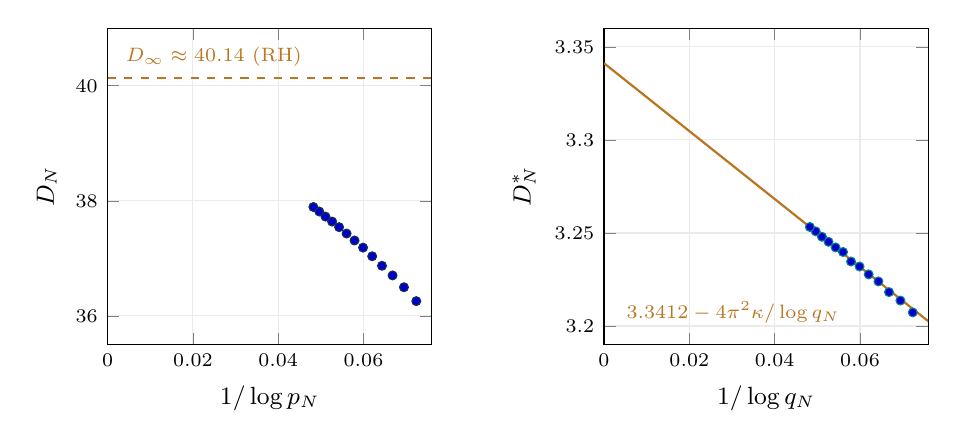
\begin{tikzpicture}
\begin{axis}[
 width=.47\textwidth,height=5.6cm,
 xmin=0,xmax=0.076,ymin=35.5,ymax=41,
 xlabel={\(1/\log p_N\)},ylabel={\(D_N\)},
 tick label style={font=\scriptsize},label style={font=\small},
 scaled x ticks=false,xtick={0,0.02,0.04,0.06},
 x tick label style={/pgf/number format/fixed},
 grid=major,grid style={black!8},mark size=1.6pt]
\addplot+[navy,only marks,mark=*] coordinates {
 (0.072382,36.256294) (0.069487,36.497673) (0.066815,36.703025)
 (0.064340,36.871051) (0.062042,37.036306) (0.059903,37.186404)
 (0.057906,37.310521) (0.056038,37.431375) (0.054287,37.542062)
 (0.052642,37.639455) (0.051093,37.725876) (0.049634,37.814290)
 (0.048255,37.892554)};
\addplot[gold,thick,dashed,domain=0:0.076] {40.14};
\node[gold,font=\scriptsize,anchor=south west] at (axis cs:0.002,40.17) {\(D_\infty\approx40.14\) (RH)};
\end{axis}
\begin{axis}[
 at={(.52\textwidth,0)},anchor=south west,
 width=.47\textwidth,height=5.6cm,
 xmin=0,xmax=0.076,ymin=3.19,ymax=3.36,
 xlabel={\(1/\log q_N\)},ylabel={\(D^*_N\)},
 tick label style={font=\scriptsize},label style={font=\small},
 scaled x ticks=false,xtick={0,0.02,0.04,0.06},
 x tick label style={/pgf/number format/fixed},
 y tick label style={/pgf/number format/fixed,/pgf/number format/precision=2},
 grid=major,grid style={black!8},mark size=1.6pt]
\addplot+[teal,only marks,mark=*] coordinates {
 (0.072382,3.207317) (0.069487,3.213689) (0.066815,3.218221)
 (0.064340,3.223955) (0.062042,3.227739) (0.059903,3.231981)
 (0.057906,3.234658) (0.056038,3.239767) (0.054287,3.242223)
 (0.052642,3.245243) (0.051093,3.247955) (0.049634,3.250851)
 (0.048255,3.253215)};
\addplot[gold,thick,domain=0:0.076] {3.3412-39.4784176*0.0461914*x};
\node[gold,font=\scriptsize,anchor=south west] at (axis cs:0.003,3.196) {\(3.3412-4\pi^2\kappa/\log q_N\)};
\end{axis}
\end{tikzpicture}
\caption{Deficits at thirteen checkpoints \(10^{6}\le X\le10^{9}\),
plotted against \(1/\log X\). Right: the prediction
\(D^*_\infty-4\pi^2\kappa/\log q_N\) with \(\kappa=2\lambda_1\). It has
no fitted slope; only the intercept is taken from Table~\ref{cl:tab:limits}.}
\label{cl:fig:limits}
\end{figure}

\subsection{The function-field analogue: here the closure is a theorem}

Let \(C/\mathbb F_q\) be a smooth projective geometrically irreducible
curve of genus \(g\). Then
\(Z_C(T)=\prod_{i=1}^{2g}(1-\alpha_iT)/((1-T)(1-qT))\) and
\(N_n=\#C(\mathbb F_{q^n})=q^n+1-\sum_i\alpha_i^n\). Let \(a_d\) be the
number of closed points of degree \(d\), so that
\(N_n=\sum_{d\mid n}da_d\). The analogue of \(p^{-1}\) is
\(q^{-\deg P}\), and the analogue of \(\log\log x\) is the harmonic
number \(H_n\). Put
\[
 S_C(n)=\sum_{d\le n}a_dq^{-d},\qquad
 E_C(n)=S_C(n)-H_n-c_C,\qquad c_C=\lim_{n\to\infty}(S_C(n)-H_n),
\]
and, with the \(x\)-measure weights \(w_n=q^{n+1}-q^{n-1}\),
\[
 D_N^C=\sum_{n=1}^Nw_n-\Bigl|\sum_{n=1}^Nw_n\,e^{2\pi\ii(S_C(n)-H_n)}\Bigr| .
\]
Again no constant is supplied.

\begin{theorem}[Function-field closure]\label{cl:thm:ff}
\leavevmode
\begin{enumerate}[label=(\alph*),itemsep=2pt]
\item \(|\alpha_i|=\sqrt q\) for all \(i\) if and only if
\(\sup_ND_N^C<\infty\).
\item The left side holds: Hasse proved it for \(g=1\) \cite{cl:hasse},
and Weil in general \cite{cl:weil}. Hence \(\sup_ND_N^C<\infty\)
unconditionally, and \(D^C_\infty-D^C_N=O_C(1/N)\).
\end{enumerate}
\end{theorem}
\begin{proof}
M\"obius inversion gives
\(na_n=N_n+\sum_{d\mid n,\,d<n}\mu(n/d)N_d\), and the inner sum is
\(O_g(q^{n/2})\). Hence
\[
 a_nq^{-n}-\frac1n=-\frac1n\sum_i\Bigl(\frac{\alpha_i}q\Bigr)^n
 +O_g\Bigl(\frac{q^{-n/2}}n\Bigr).
\]
If \(|\alpha_i|=\sqrt q\), then
\(|E_C(n)|\le\sum_{d>n}|a_dq^{-d}-1/d|\ll_g q^{-n/2}/n\). Therefore
\(\sum_nw_n|e^{2\pi\ii E_C(n)}-1|^2\ll\sum_nn^{-2}<\infty\), with tail
\(O(1/N)\), and Lemma~\ref{pc:lem:variance} applies.

Conversely, suppose \(r=\max_i|\alpha_i|/q>q^{-1/2}\). The terms with
\(|\alpha_i|=rq\) dominate and give
\(E_C(n)=n^{-1}r^n\bigl(\sum_ic_iz_i^n+o(1)\bigr)\), with distinct
\(|z_i|=1\) and \(c_i\ne0\). A nondegenerate exponential sum
\(\sum_ic_iz_i^n\) has positive mean square. Hence
\(w_nE_C(n)^2\gg(r^2q)^n/n^2\) on a set of \(n\) of positive density,
and \(\mathcal J=\infty\).
\end{proof}

For \(g=1\), the input in (b) is Hasse's inequality \(|a|\le2\sqrt q\),
where \(a=q+1-\#C(\mathbb F_q)\). Its standard proof shows that the
degree form
\(\deg(m-n\pi)=m^2-a\,mn+q\,n^2\ge0\) on \(\operatorname{End}(C)\) is
positive semidefinite. It is positive definite, with elliptic level curves, when $a^2<4q$, and degenerate when $a^2=4q$. The discriminant
condition \(a^2\le4q\) then places the Frobenius eigenvalues on the
circle \(|\alpha|=\sqrt q\). In this analogue, therefore, the closure
missing from Section~\ref{pc:sec:open} is supplied by the nonnegative degree form, including its degenerate equality case. Both cases give the required spectral modulus. Weil's
proof for general \(g\) uses the positivity of the
Castelnuovo--Severi, or Hodge index, form. The number-field counterpart
of that positivity is Weil's explicit-formula positivity, which is
equivalent to RH \cite{cl:bombieri-lagarias}.

\begin{table}[htbp]
\centering
\small
\begin{tabular}{@{}lrrrrrr@{}}
\toprule
\(N\) & 5 & 10 & 20 & 40 & 60 & 140\\
\midrule
\(D^C_N\), \(y^2=x^3+x+1\) over \(\mathbb F_5\)
 & 27.738 & 33.164 & 35.216 & 36.191 & 36.536 & 36.887\\
\(D_N\), fake \(|\alpha|=5^{0.7}\)
 & 108.5 & 808.5 & \(1.28\cdot10^{5}\) & \(1.18\cdot10^{10}\)
 & \(2.03\cdot10^{15}\) & --\\
\bottomrule
\end{tabular}
\caption{The curve has \(a=-3\) and \(a^2-4q=-11<0\), so its degree form
is an ellipse; \(|q^{N/2}NE_C(N)|\le1.22\) for \(5\le N\le140\), and
\(D^C_N\) converges. Replacing \(\alpha\) by \(5^{0.7}e^{1.1\ii\,}\)
violates the analogue of RH, and the deficit grows geometrically.
Exact integer point counts were used, with 260-digit arithmetic.}
\label{cl:tab:ff}
\end{table}

\subsection{What remains}

The attempt ends where Section~\ref{pc:sec:open} ended, with a sharper
description of the gap.
\begin{itemize}[itemsep=3pt]
\item Every representation used here is equivalent to RH and supplies
no bound by itself (Proposition~\ref{cl:prop:invariance}). This includes
the circle, the fixed and spectral ellipses, the Cayley/Hardy disk,
Li's coordinate and Jensen's formula.
\item Unconditionally, \(D_N=o(p_N)\) with the Vinogradov--Korobov
saving (Theorem~\ref{cl:thm:VK}). A power saving \(D_N\ll p_N^{1-\delta}\)
is equivalent to a zero-free half-plane
(Theorem~\ref{cl:thm:dictionary}). The unrefereed 2026 claims would give
the exponent \(3/4\).
\item Under the RH and simplicity model, the extrapolations are near
$40.14$ for $D_\infty$ and $3.3412$ for $D^*_\infty$.
These are not upper-bound certificates. The conditional tail theorem describes
a logarithmic approach (Proposition~\ref{cl:prop:density} and
Remark~\ref{cl:cor:K}).
\item In the function-field analogue the same deficit is bounded, and
the bound comes from the nonnegative degree form and the Hasse--Weil theorem
(Theorem~\ref{cl:thm:ff}). For \(\mathbb Q\) the corresponding positivity
statements are Weil's criterion and Zhao's one-sided integral
criterion. Both are equivalent to RH.
\end{itemize}
No unconditional bound of the required strength is supplied here.


% Consolidated source: Prime_Reciprocal_Circles_Eighty_Methods.tex, section-index 6
\section{Independent interval evaluation of finite deficits}
The original prime-endpoint deficit was recomputed by a direct
vector sum using outward-rounded \texttt{mpmath.iv} intervals at
40 decimal places. This uses no centering constant, no quadrature,
and a different summation identity from the manuscript's stable
nonnegative-update calculation. A deterministic Eratosthenes sieve
includes the next prime needed for the final weight. For display,
the raw enclosures have been widened to the following shorter intervals:
\begin{center}
\small
\begin{tabular}{@{}rrrr@{}}
\toprule
$X$ & $p_N$ & $W_N$ & Enclosure for $D_N$\\
\midrule
$10$ & $7$ & $13$ & $[1.969759465990,\ 1.969759465991]$\\
$10^2$ & $97$ & $193$ & $[16.710860675974,\ 16.710860675975]$\\
$10^3$ & $997$ & $2001$ & $[26.969965365289,\ 26.969965365290]$\\
$10^4$ & $9973$ & $19975$ & $[32.298046003525,\ 32.298046003526]$\\
$10^5$ & $99991$ & $199989$ & $[34.913607775328,\ 34.913607775329]$\\
$10^6$ & $999983$ & $1999981$ & $[36.256293902575,\ 36.256293902576]$\\
$10^7$ & $9999991$ & $20000005$ & $[37.036305899751,\ 37.036305899752]$\\
\bottomrule
\end{tabular}
\end{center}
The first six reproduce the original checkpoints, while the last
extends the cutoff by a factor of ten. These are reproducible
interval-library enclosures, not a formally verified proof of the
software's implementation. The complete interval source is embedded in Appendix~\ref{e80:app:code}; the intervals above are widened from its output.

Monotonicity gives the finite lower bound
$\sup_ND_N>37.03630589975147353138$, subject to the computational
certificate just described. If RH is assumed, the supremum is
$D_\infty$, and the manuscript's identity gives the corresponding
weighted circle energy greater than $74.07261179950294706276$.
Neither statement is an upper bound, and neither verifies RH.

A separate non-certified long-double experiment evaluated the new
integer-window criterion through $m=4{,}194{,}303$. It gave
$D_{21}^*\approx15.703975172$, $L_{21}\approx5.127737034$, and
$d_{20}\approx0.011272267$. These values concern integer sampling,
not the differently weighted prime-endpoint deficit; their numerical
scales must not be conflated. Agreement with the finite inequalities
is a consistency test, not evidence controlling all subsequent windows.
\paragraph{A rigorously certified obstruction to local monotonicity.}
Although the cumulative global deficit is nondecreasing, the new
local deficits are not nonincreasing. An independent calculation
using only exact Python integers, with no floating-point operations
or external numerical packages, proves
\[
\begin{aligned}
 d_5\in[0.17426320563310160979,0.17426320563310160980],\\
 d_6\in[0.18116395307408146771,0.18116395307408146772].
\end{aligned}
\]
In particular $d_6>d_5$. The exact-integer program in Appendix~\ref{e80:app:rational} represents every interval as
$[a/10^{70},b/10^{70}]$, rounding each integer operation outwards.
For logarithms, it first scales the argument into $[1,2)$ and uses
\[
 \log y=2\sum_{j=0}^{99}\frac{t^{2j+1}}{2j+1}+R,
 \qquad t=\frac{y-1}{y+1},\qquad
 |R|\le\frac{9}{4\cdot201\cdot3^{201}},
\]
with the appropriate integer multiple of $\log2$ restored.
Monotonicity of the logarithm handles interval endpoints.
Machin's identity $\pi=16\arctan(1/5)-4\arctan(1/239)$ is
combined with 100-term alternating series and their next-term bounds.
The sine and cosine Taylor polynomials have degrees 161 and 160;
the code verifies $|\text{phase}|\le6$ and bounds the respective
remainders by $6^{162}/162!$ and $6^{161}/161!$.
Square-root bounds use integer square root. The output records exact
integer numerators and verifies that the upper numerator for $d_5$
is strictly less than the lower numerator for $d_6$. This is a
fully specified finite rational certificate; it is not an estimate
of subsequent deficits and does not settle their boundedness.

The larger interval run used Python 3.12.14, NumPy 2.3.5, and
mpmath 1.3.0, with \texttt{iv.dps=40} decimal interval precision.


% Consolidated source: Prime_Reciprocal_Circles_Further_Closures.tex, section-index 7
\section{Finite checks and the role of computation}
\label{fc:checks:section}

The new finite calculations use 90 decimal digits in \texttt{mpmath}.
They are checks of algebra and normalization, not interval certificates
of an infinite assertion.  The distinct exception is the exact rational
certificate following Proposition~\ref{fc:tails:kappabound}.
All code needed for the tables is embedded in this TeX file.

\subsection{The actual degree-four prime polynomials}

The prime index $N$ is used, not a cutoff $x$.  The sieve includes
$p_{N+1}$ so that the final original weight is correct.
The normal equations for $P_{4,N}$ are solved directly, and its norm
is independently evaluated as a positive weighted sum.
The deficit is computed from a positive variance sum to avoid subtracting
two nearly equal large numbers.  Neither computation supplies $\BP$.

\begin{table}[htbp]
\centering\small
\begin{tabular}{@{}rrrrrr@{}}\toprule
$N$ & $p_N$ & $D_N$ & $H_{4,N}$ & $\rho_{1,N}$ & $\rho_{2,N}$\\
\midrule
100 & 541 & 24.716380 & 4.912210 & 0.99763801 & 0.96186498\\
1000 & 7919 & 31.902292 & 8.792997 & 0.99960317 & 0.95471782\\
10000 & 104729 & 34.944886 & 10.741125 & 0.99995002 & 0.95455190\\
\bottomrule\end{tabular}
\caption{Finite values for the original prime weights and phases.
The final two columns are the largest and second largest root moduli,
not zeta-zero locations.}\label{fc:checks:primetable}
\end{table}

Every displayed finite root lies inside the disk, as expected from
the finite OPUC theory.  What is unproved is a gap for the second root
that persists for all sufficiently large $N$.
At the largest sample, the bound in
Proposition~\ref{fc:further:finitegap} is about $4.92\cdot10^7$, whereas
$D_N$ is about $34.94$.  Thus the general root-gap inequality is
valid but loose in this numerical example; it is not presented as
a good numerical estimate for $D_\infty$.

\begin{figure}[htbp]\centering
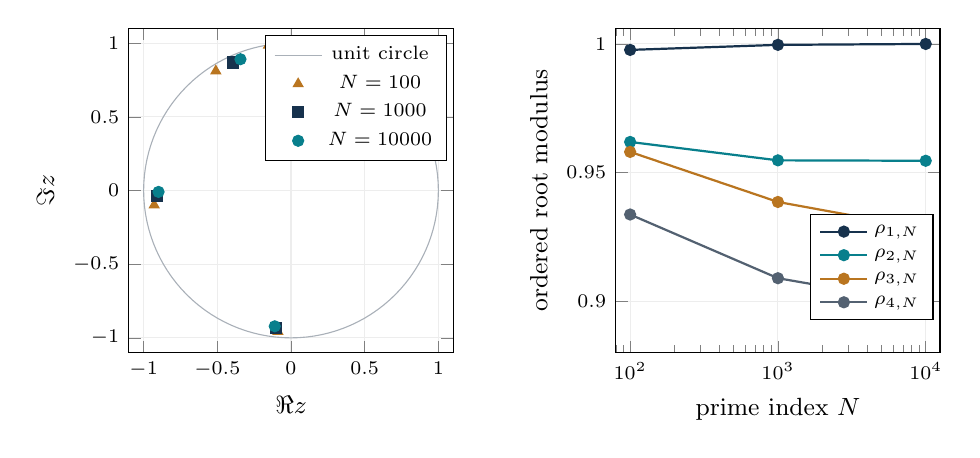
\begin{tikzpicture}
\begin{axis}[width=.47\textwidth,height=.47\textwidth,
 axis equal image,xmin=-1.1,xmax=1.1,ymin=-1.1,ymax=1.1,
 xlabel={$\Re z$},ylabel={$\Im z$},
 tick label style={font=\scriptsize},label style={font=\small},
 legend style={font=\scriptsize,at={(.98,.98)},anchor=north east},
 grid=major,grid style={black!7}]
\addplot[inkgray!50,domain=0:360,samples=121,no marks] ({cos(x)},{sin(x)});
\addlegendentry{unit circle}
\addplot[only marks,gold,mark=triangle*,mark size=2pt] coordinates {(-0.152761259802,0.985873010478) (-0.088472097066,-0.957787513752) (-0.510150589078,0.810866661177) (-0.928429221518,-0.098753223825)};
\addlegendentry{$N=100$}
\addplot[only marks,navy,mark=square*,mark size=2pt] coordinates {(-0.089150954501,0.995619705241) (-0.395354497419,0.869011466011) (-0.102962717501,-0.932879789780) (-0.908189178474,-0.036227366662)};
\addlegendentry{$N=1000$}
\addplot[only marks,teal,mark=*,mark size=2pt] coordinates {(-0.075942305282,0.997062089425) (-0.342879780420,0.890843861352) (-0.110256634999,-0.921502560336) (-0.898908869863,-0.009510860087)};
\addlegendentry{$N=10000$}
\end{axis}
\begin{axis}[at={(.51\textwidth,0)},anchor=south west,
 width=.47\textwidth,height=.47\textwidth,
 xmode=log,xmin=80,xmax=12500,ymin=.88,ymax=1.006,
 xlabel={prime index $N$},ylabel={ordered root modulus},
 tick label style={font=\scriptsize},label style={font=\small},
 legend style={font=\scriptsize,at={(.98,.1)},anchor=south east},
 grid=major,grid style={black!7}]
\addplot[navy,thick,mark=*,mark size=1.8pt] coordinates {(100,0.997638008140) (1000,0.999603166337) (10000,0.999950020701)};
\addlegendentry{$\rho_{1,N}$}
\addplot[teal,thick,mark=*,mark size=1.8pt] coordinates {(100,0.961864976730) (1000,0.954717815214) (10000,0.954551899653)};
\addlegendentry{$\rho_{2,N}$}
\addplot[gold,thick,mark=*,mark size=1.8pt] coordinates {(100,0.957997059361) (1000,0.938544630465) (10000,0.928075155505)};
\addlegendentry{$\rho_{3,N}$}
\addplot[inkgray,thick,mark=*,mark size=1.8pt] coordinates {(100,0.933666438609) (1000,0.908911440127) (10000,0.898959183044)};
\addlegendentry{$\rho_{4,N}$}
\end{axis}\end{tikzpicture}
\caption{Left: roots of the computed degree-four prime extremizers.
Right: their ordered moduli at three finite indices.
The lines join observations only; they are not estimates of future
behavior or certified limiting root gaps.}\label{fc:checks:primefigure}
\end{figure}

The relative least-squares orthogonality residual is below
$7\cdot10^{-88}$ in these runs.  Evaluation of the computed roots
in the polynomial gives residuals below $4\cdot10^{-91}$.
For the $r=3$ spectral matrices, the finite leakage identity and its
independent harmonic expression agree to absolute error below
$1.2\cdot10^{-84}$.
The ratios $\mathcal T_{3,N}/\mathcal L_{3,N}$ are respectively
$3.89775697$, $3.98992652$, and $3.99912027$; their convergence to four
is predicted by an unconditional theorem for convergent phase sequences,
so it does not constitute evidence resolving RH.

\subsection{Curve-tail coefficients}

We evaluate closed-point counts using integer recurrences and
M\"obius inversion, then compute the errors by backward summation
of their tails.  The sum is carried 160 degrees past the largest
displayed cutoff.  Stable phase differences use \texttt{expm1},
and the deficit is recovered through the variance identity.
The quantity
\[
 2N\{D^C_{2N}-D^C_N\}
\]
must tend to $\mathcal K_C$, by Theorem~\ref{fc:ff:tail}; this comparison
requires no extrapolated value of $D^C_\infty$.

\begin{table}[htbp]\centering\small
\begin{tabular}{@{}lrrr@{}}\toprule
Data & $\mathcal K_C$ & $2N(D_{2N}-D_N)$ & $\mathcal K_C^*$\\
 & (exact formula, decimal) & at $N=800$ & (exact formula, decimal)\\
\midrule
$q=5$, $a=-3$ & 38.820444 & 38.845534 & 21.055156\\
$q=3$, $a=0$ & 52.637890 & 52.564379 & 26.318945\\
$q=9$, $a=6$ & 276.897235 & 276.842347 & 175.459634\\
$q=5$, genus zero & 17.765288 & 17.759789 & 0.000000\\
\bottomrule\end{tabular}
\caption{The curve-tail constant compared with finite differences.
An $O(1/N)$ error in the middle column follows from the proved
$O(1/N^2)$ remainder of the deficit tail.}\label{fc:checks:fieldtable}
\end{table}

The $q=9$, trace-six spectral data test the repeated-root and
prime-square resonance case.  The genus-zero row tests the nonzero
prime-square coefficient even when there are no Frobenius roots.
The prime-power variant has zero $1/N$ coefficient in genus zero,
and its finer behavior is the separate formula \eqref{fc:ff:genuszero}.


% Consolidated source: Prime_Reciprocal_Circles.tex, section-index 20
\section{Finite experiments and what they verify}\label{pc:sec:numerics}

The computations in this section are finite numerical experiments.
They are not interval-certified, and they do not establish any
infinite convergence claim. The equations proved above are exact;
the displayed decimals here are approximations.

\subsection{Continuous energies}

We sieved primes through \(10^6\) and evaluated each prime gap
separately, so no quadrature panel crossed a discontinuity of \(S\).
For each cutoff, Gauss--Legendre quadrature of orders \(16\) and
\(32\) was compared. The largest absolute difference among the
reported energy values was below \(6\cdot10^{-14}\).
That agreement is a numerical consistency check, not a rigorous
quadrature-error bound.

Let \(J_{\rm circ}(X)=\int_2^X|Z(x)-1|^2\dd x\) and let
\(J_{\rm ell}(X)\) use axes \(a=2,b=1/2\) in
Theorem~\ref{pc:thm:energy}.
\begin{table}[htbp]
\centering
\small
\begin{tabular}{@{}rrrr@{}}
\toprule
\(X\) & \(I(X)\) & \(J_{\rm circ}(X)\) & \(J_{\rm ell}(X)\)\\
\midrule
\(10\)      &0.4528982208&12.3501439535&28.9243950387\\
\(10^2\)    &0.6453466953&19.7963685485&32.3999690652\\
\(10^3\)    &0.7183439651&22.6756655349&33.1480535456\\
\(10^4\)    &0.7541530540&24.0893056345&33.5019817574\\
\(10^5\)    &0.7745490579&24.8945062699&33.7032968338\\
\(10^6\)    &0.7879412220&25.4232076629&33.8354727627\\
\bottomrule
\end{tabular}
\caption{Finite continuous energies. Distinct initial behavior is
compatible with equivalent tail-convergence criteria.}
\label{pc:tab:energies}
\end{table}

\subsection{The constant-free deficit}

The deficit was accumulated using the nonnegative update
\eqref{pc:eq:dupdate}, with extended-precision floating-point
arithmetic. The next prime after each cutoff is needed for the
last weight \(w_N\). Direct subtraction and the variance identity
were used as independent numerical checks.

\begin{table}[htbp]
\centering
\small
\begin{tabular}{@{}rrrrr@{}}
\toprule
Cutoff \(X\)&Last prime \(p_N\)&\(W_N\)&\(D_N\)&\(\mathcal J_N\)\\
\midrule
\(10\)&7&13&1.9697594660&34.1413094763\\
\(10^2\)&97&193&16.7108606760&60.8759929534\\
\(10^3\)&997&2,001&26.9699653653&68.7831808384\\
\(10^4\)&9,973&19,975&32.2980460035&72.0512604990\\
\(10^5\)&99,991&199,989&34.9136077753&73.7657173538\\
\(10^6\)&999,983&1,999,981&36.2562939026&74.8491148279\\
\bottomrule
\end{tabular}
\caption{The deficit does not use \(\BP\).
The comparison column
\(\mathcal J_N=\sum_{n=2}^Nw_n|U_n-e^{2\pi\ii\BP}|^2\)
does use it. At finite \(N\), \(2D_N\le\mathcal J_N\);
equality is a limit statement under RH.}
\label{pc:tab:deficits}
\end{table}

\begin{figure}[htbp]
\centering
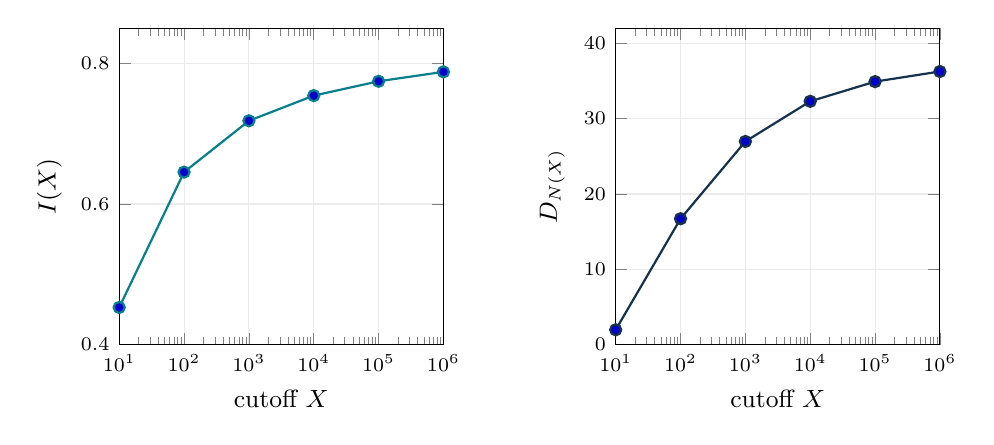
\begin{tikzpicture}
\begin{axis}[
 width=.47\textwidth,height=5.6cm,
 xmode=log,log basis x=10,
 xmin=10,xmax=1000000,ymin=.4,ymax=.85,
 xlabel={cutoff \(X\)},ylabel={\(I(X)\)},
 tick label style={font=\scriptsize},
 label style={font=\small},
 grid=major,grid style={black!8},
 mark size=2pt]
\addplot+[teal,thick,mark=*] coordinates {
 (10,.4528982208)(100,.6453466953)
 (1000,.7183439651)(10000,.7541530540)
 (100000,.7745490579)(1000000,.7879412220)};
\end{axis}
\begin{axis}[
 at={(.52\textwidth,0)},anchor=south west,
 width=.47\textwidth,height=5.6cm,
 xmode=log,log basis x=10,
 xmin=10,xmax=1000000,ymin=0,ymax=42,
 xlabel={cutoff \(X\)},ylabel={\(D_{N(X)}\)},
 tick label style={font=\scriptsize},
 label style={font=\small},
 grid=major,grid style={black!8},
 mark size=2pt]
\addplot+[navy,thick,mark=*] coordinates {
 (10,1.969759466)(100,16.710860676)
 (1000,26.9699653653)(10000,32.2980460035)
 (100000,34.9136077753)(1000000,36.2562939026)};
\end{axis}
\end{tikzpicture}
\caption{Reported checkpoints joined for readability.
The visible flattening over this finite range does not prove
boundedness. Here \(N(X)=\pi(X)\).}
\end{figure}

\subsection{Initial Laguerre coefficients}

For \(\alpha=1\), a high-precision evaluation of
\eqref{pc:eq:Fcompute}--\eqref{pc:eq:coeffderivs}, checked against
derivatives of the generating function, gives:
\begin{table}[htbp]
\centering
\begin{tabular}{@{}rr@{}}
\toprule
\(n\)&\(a_n^{(1)}\)\\
\midrule
0&\(\phantom{-}0.346934737830795621\)\\
1&\(-0.661616469769648581\)\\
2&\(\phantom{-}0.225894182779432296\)\\
3&\(-0.140258082155750076\)\\
4&\(\phantom{-}0.228257943870596736\)\\
5&\(-0.040192481906854658\)\\
6&\(\phantom{-}0.163353841105629616\)\\
\bottomrule
\end{tabular}
\caption{Approximate initial coefficients, not certified intervals.}
\end{table}
Their squared sum is approximately
\[
 \sum_{n=0}^6|a_n^{(1)}|^2
 =0.709202178753600527.
\]
These are global transform coefficients, so their finite partial sum
is not an integral truncated at \(x=10^6\).
Under RH, all coefficient squares sum to \(I(\infty)\), but neither
the printed coefficients nor Table~\ref{pc:tab:energies} controls the
remaining tail. Appendix~\ref{pc:app:certification} supplies explicit
bounds that can be used to certify individual finite calculations.


\subsection{Finite checks of the harmonic and determinant transfers}
\label{pc:m80:numerics}

The following values use the original prime vectors and weights.
The pair definition of \(C_{4,N}\) was evaluated independently of
its alternating harmonic formula. The least-squares value \(H_{4,N}\)
was also compared with the Gram determinant ratio. Calculations used
90 decimal digits; they are floating-point checks, not interval
certificates. No infinite bound is inferred from the table.

\begin{table}[htbp]
\centering\small
\begin{tabular}{rrrrr}
\toprule
\(N\) & \(p_N\) & \(D_N\) & \(C_{4,N}\) & \(H_{4,N}\)\\
\midrule
8 & 19 & 7.16815104 & 225.62037355 & 0.14477688\\
16 & 53 & 13.36793576 & 510.93018613 & 0.76241711\\
32 & 131 & 18.13936274 & 700.80614780 & 2.04459049\\
64 & 311 & 22.31007541 & 828.12192867 & 3.75468037\\
128 & 719 & 25.82085230 & 909.14157506 & 5.47180933\\
\bottomrule
\end{tabular}
\caption{Finite checks of the original deficit, fourth pair moment,
and degree-four monic extremal norm.}
\label{pc:m80:tablechecks}
\end{table}

Across all tested prefixes and moment orders \(1\le m\le4\), the
maximum absolute discrepancy in the harmonic identity was less than
\(10^{-86}\). The determinant-ratio discrepancy was also less than
\(10^{-86}\). The finite H\"older bridge was satisfied at every
tested prefix. Its values grow much faster than the observed deficit;
it is a valid upper bound, not an effective numerical estimate of the
remaining constant. The nonmonotonicity example gives exactly
\(9/2\) followed by \(11/3\), as stated in
Remark~\ref{pc:m80:rem:nonmonotone}.
The complete calculation is embedded in Appendix~\ref{pc:m80:checkcode}.


% Consolidated source: Prime_Reciprocal_Circles.tex, section-index 22
\section{Eighty methods: complete transfer and source audit}
\label{pc:m80:audit}

Every numbered example supplied for this extension appears below.
An application is counted as a proved transfer only when its hypotheses
have been checked in the present construction. Otherwise the row states
the additional mathematical input required. The original target remains
\(\sup_ND_N<\infty\). A different finite-moment threshold, a finite
computation, or an existence theorem is not substituted for that target.

The links identify the supplied source or a primary replacement.
``Access'' distinguishes a full text, an abstract or author survey,
indexed source text, and an unavailable original. This is a targeted
mechanism audit, not an independent reproduction of eighty original
proofs. Several entries share one proof technology; the eighty examples
do not provide eighty independent estimates for the prime error.

The connections and missing-hypothesis statements in the right column
are deductions in this note. They are not claims made by the authors
of the linked papers. Complete proofs of the successful transfers are
in Sections~\ref{pc:m80:pairenergy}--\ref{pc:m80:topology}.

\subsection{Fourier analysis, circle integrals, and determinants: 1--20}
\begingroup
\footnotesize
\setlength{\tabcolsep}{5pt}
\renewcommand{\arraystretch}{1.10}
\begin{longtable}{@{}>{\raggedright\arraybackslash}p{0.255\textwidth}>{\raggedright\arraybackslash}p{0.705\textwidth}@{}}
\toprule
\textbf{Method and source} & \textbf{Mechanism, attempted transfer, and outcome}\\
\midrule\endfirsthead
\toprule
\textbf{Method and source} & \textbf{Mechanism, attempted transfer, and outcome}\\
\midrule\endhead
\midrule\multicolumn{2}{r}{\scriptsize Continued on next page}\\\endfoot
\bottomrule\endlastfoot
\textbf{1. Ternary Goldbach}\par\smallskip \href{https://arxiv.org/abs/1404.2224}{Source}\par\smallskip {\scriptsize\textit{Access:} Primary author overview opened; the whole multi-paper proof and computation were not independently reproduced.} & \textbf{Mechanism.} Helfgott combines major-arc estimates, minor-arc bounds, the large sieve, and finite verification to prove the three-prime theorem for odd integers greater than five.\par\smallskip\textbf{Transfer.} Apply Fourier orthogonality to the dyadic polynomials \(A_j\) whose coefficients are E(n). Both arc regions would need a uniform or summable quadratic budget.\par\smallskip\textbf{Outcome.} An exact Fourier criterion is obtained in the main text. Published threefold-convolution estimates do not provide the required bound for these error coefficients.\\[6pt]
\midrule
\textbf{2. Integer partitions}\par\smallskip \href{https://pmc.ncbi.nlm.nih.gov/articles/PMC1076871/}{Source}\par\smallskip {\scriptsize\textit{Access:} User's circle-method overview was read. Rademacher's 1937 primary record was retrieved; full PMC access hit a bot check.} & \textbf{Mechanism.} Cauchy coefficient extraction and the modular transformation of the partition generating function yield asymptotics and Rademacher's convergent exact series.\par\smallskip\textbf{Transfer.} A comparable transformation law for the relevant prime-error generating function would be needed, with rigorous uniform control of the transformed remainder.\par\smallskip\textbf{Outcome.} No such modular law follows from circle integration alone. The finite Laguerre-polynomial construction instead gives an exact Szego determinant identity, with its uniform constant still unknown.\\[6pt]
\midrule
\textbf{3. Waring representation counts}\par\smallskip \href{https://personal.science.psu.edu/rcv4/568s20/568chapter22.pdf}{Source}\par\smallskip {\scriptsize\textit{Access:} Vaughan's author-hosted Waring notes were read; the user's Encyclopedia overview was also checked.} & \textbf{Mechanism.} The circle method extracts representations by powers and bounds minor arcs; singular series and singular integrals supply the main term under the relevant hypotheses.\par\smallskip\textbf{Transfer.} A prime-energy violation would need to force an impossible representation count, or the relevant exponential-sum bounds would have to control the dyadic error norms uniformly.\par\smallskip\textbf{Outcome.} The coefficient-extraction step transfers exactly, but no such arithmetic implication or bound has been established. Hilbert's prior existence proof is a separate method.\\[6pt]
\midrule
\textbf{4. Sixteen fourth powers}\par\smallskip \href{https://personal.science.psu.edu/rcv4/568s20/568chapter22.pdf}{Source}\par\smallskip {\scriptsize\textit{Access:} Supplied author lecture notes opened. The number is G(4), the eventual threshold, not the all-integer Waring number g(4).} & \textbf{Mechanism.} The exact eventual threshold G(4)=16 combines analytic representation estimates with congruence obstructions that show optimality.\par\smallskip\textbf{Transfer.} The analogue would be a sharp minor-arc bound for the original quadratic error, with local arithmetic conditions strong enough to prevent remaining exceptional concentration.\par\smallskip\textbf{Outcome.} No threshold from additive fourth powers bounds our second moment. The four-harmonic statistic bounded under $(H_b)$ has eighth-order contact and a different exact zero-location threshold.\\[6pt]
\midrule
\textbf{5. Five prime squares}\par\smallskip \href{https://arxiv.org/abs/1711.08578}{Source}\par\smallskip {\scriptsize\textit{Access:} Primary paper opened. The linked proof is a transference proof; it should not be described as merely the original circle-method proof.} & \textbf{Mechanism.} The linked paper gives an L-function-free transference proof of Hua's theorem for sufficiently large N congruent to 5 modulo 24, using a sieve majorant and pseudorandomness estimates.\par\smallskip\textbf{Transfer.} A dense-model or transference argument would need a verified majorant and pseudorandom estimates for the actual centered-error observable, together with a quantitative inverse comparison.\par\smallskip\textbf{Outcome.} The theorem's admissible congruence class and its pseudorandomness hypotheses do not automatically control \(D_N\). Higher moments can remain finite while its quadratic energy diverges.\\[6pt]
\midrule
\textbf{6. Roth's three-term progressions}\par\smallskip \href{https://doi.org/10.1112/jlms/s1-28.1.104}{Source}\par\smallskip {\scriptsize\textit{Access:} Original 1953 publisher metadata retrieved; direct full text blocked. The supplied 2018 article is a Roth obituary, not the original proof.} & \textbf{Mechanism.} Fourier analysis detects a large coefficient when a dense set has too few progressions; a density increment then forces a contradiction after iteration.\par\smallskip\textbf{Transfer.} One would need a density or bounded potential attached to prime-error blocks, and a quantitatively controlled increment caused by excessive variance.\par\smallskip\textbf{Outcome.} The block merger identity is exact, but no bounded density parameter or exhausting increment argument has been constructed for the original prime sequence.\\[6pt]
\midrule
\textbf{7. Square differences in dense sets}\par\smallskip \href{https://doi.org/10.1007/BF01896079}{Source}\par\smallskip {\scriptsize\textit{Access:} Original Sarkozy reference identified, full DOI access unavailable. Scope corroborated by primary difference-set research; the supplied MathWorld entry is secondary.} & \textbf{Mechanism.} Fourier estimates for square exponential sums and density increment, or ergodic recurrence, force a square difference in a set of positive upper density.\par\smallskip\textbf{Transfer.} A high-error subset would need positive density with a quantitatively controlled square-difference obstruction derived from the prime-reciprocal recurrence.\par\smallskip\textbf{Outcome.} No such forbidden-difference implication is present. An energy can diverge on a set of density zero, so the qualitative density theorem alone cannot settle the required norm.\\[6pt]
\midrule
\textbf{8. Prime-minus-one differences}\par\smallskip \href{https://arxiv.org/abs/0710.0644}{Source}\par\smallskip {\scriptsize\textit{Access:} Primary Ruzsa-Sanders abstract opened. The user's Oxford link is a research seminar announcement; it was also read.} & \textbf{Mechanism.} Shifted-prime exponential sums, Fourier concentration and density increment control sets avoiding differences p-1; Ruzsa and Sanders give a quantitative bound.\par\smallskip\textbf{Transfer.} Large prime-circle errors would need to create a sufficiently dense difference-avoiding set, or the shifted-prime estimates would need to control the actual error coefficients directly.\par\smallskip\textbf{Outcome.} The required connection to a forbidden difference has not been proved. A theorem about existence of one additive configuration is not a uniform upper bound for all weighted error blocks.\\[6pt]
\midrule
\textbf{9. Birch's systems of forms}\par\smallskip \href{https://doi.org/10.1098/rspa.1962.0007}{Source}\par\smallskip {\scriptsize\textit{Access:} Original DOI/full text unavailable; bibliographic and abstract text retrieved. Related author research on forms was opened. No full fresh reading of Birch's proof is claimed.} & \textbf{Mechanism.} A torus integral, Weyl differencing and local densities give asymptotic solution counts when the singular locus has sufficiently large codimension and the required local solubility holds.\par\smallskip\textbf{Transfer.} An explicit system of fixed-degree forms would have to encode a prime-energy violation while satisfying the rank and local hypotheses uniformly in the index.\par\smallskip\textbf{Outcome.} A multitorus coordinate change supplies no such system. The original analytic target has no verified reduction to these finite-dimensional polynomial constraints.\\[6pt]
\midrule
\textbf{10. Cubic forms in many variables}\par\smallskip \href{https://www.math.purdue.edu/~twooley/publ/2003pcub.pdf}{Source}\par\smallskip {\scriptsize\textit{Access:} The supplied SciXplorer page had a bot wall. Dietmann-Wooley's primary paper was opened and explicitly records Davenport's sixteen-variable result.} & \textbf{Mechanism.} Davenport's circle-method estimates, with arithmetic and geometric reductions, show that sixteen variables suffice for a rational cubic form to have a nontrivial rational zero.\par\smallskip\textbf{Transfer.} One needs a faithful polynomial encoding in which the existence or impossibility of a cubic zero gives a uniform prime-error estimate.\par\smallskip\textbf{Outcome.} Adding auxiliary variables can make a new equation soluble without retaining any bound for the original observable. No faithful encoding with the required quantitative comparison is available.\\[6pt]
\midrule
\textbf{11. Longest increasing subsequences}\par\smallskip \href{https://arxiv.org/abs/math/9810105}{Source}\par\smallskip {\scriptsize\textit{Access:} Primary arXiv record and the relevant method description opened. No identity with the random permutation model is assumed.} & \textbf{Mechanism.} Baik-Deift-Johansson use a Toeplitz determinant representation, orthogonal polynomials and Riemann-Hilbert asymptotics to determine the limiting distribution.\par\smallskip\textbf{Transfer.} Form the Toeplitz moment matrix of the original positive atomic prime measure and study its monic extremal polynomial norms.\par\smallskip\textbf{Outcome.} This produces the proved hierarchy \(H_m\): boundedness is exactly the 2m-moment threshold. \(H_4\) is bounded using the stated zero-free input; \(H_1\) remains the RH-equivalent variance.\\[6pt]
\midrule
\textbf{12. Fisher-Hartwig asymptotics}\par\smallskip \href{https://annals.math.princeton.edu/2011/174-2/p12}{Source}\par\smallskip {\scriptsize\textit{Access:} Primary Annals theorem record opened; its scope is retained rather than calling every Fisher-Hartwig regime solved.} & \textbf{Mechanism.} The cited theorem analyzes Toeplitz and related determinants with controlled root and jump singularities, using orthogonal-polynomial and Riemann-Hilbert methods within stated parameter ranges.\par\smallskip\textbf{Transfer.} The prime-dependent symbols would need a justified singularity model and estimates uniform as the number or location of singularities varies.\par\smallskip\textbf{Outcome.} Finite determinant identities transfer, but the cited fixed-symbol theorem does not furnish a uniform bound over all prime prefixes. The exact double-index criterion isolates that missing uniformity.\\[6pt]
\midrule
\textbf{13. Dyson's large-gap constant}\par\smallskip \href{https://arxiv.org/abs/math/0401258}{Source}\par\smallskip {\scriptsize\textit{Access:} Primary arXiv paper record opened.} & \textbf{Mechanism.} Krasovsky analyzes orthogonal polynomials on an arc and Toeplitz determinants to compute the constant in the large-gap asymptotic.\par\smallskip\textbf{Transfer.} An arc-supported prime measure would need uniformly controlled weights and a matching asymptotic regime; the constant must then dominate the original quadratic deficit.\par\smallskip\textbf{Outcome.} The atomic prime measure and its increasing total mass are not the fixed ensemble in that theorem. Our degree-four determinant ratio closes a different observable; no original constant follows.\\[6pt]
\midrule
\textbf{14. One-dimensional Bose occupations}\par\smallskip \href{https://arxiv.org/abs/1403.3639}{Source}\par\smallskip {\scriptsize\textit{Access:} Claeys-Krasovsky primary record, revised version, opened. The application concerns the specified model and conjecture.} & \textbf{Mechanism.} Uniform Toeplitz asymptotics for two merging Fisher-Hartwig singularities resolve the cited occupation-number conjecture for the impenetrable Bose gas.\par\smallskip\textbf{Transfer.} A proven correspondence between the arithmetic symbol and the physical symbol, including uniform control of its merging parameter, is required.\par\smallskip\textbf{Outcome.} No physical-model identity has been established. The useful imported operation is finite positive Toeplitz optimization, whose exact arithmetic threshold is proved separately.\\[6pt]
\midrule
\textbf{15. A random-matrix second moment}\par\smallskip \href{https://arxiv.org/abs/1403.3639}{Source}\par\smallskip {\scriptsize\textit{Access:} Same primary paper as item 14; this is a separate application, not a second independent proof technology.} & \textbf{Mechanism.} The same merging-singularity analysis evaluates a particular averaged characteristic-polynomial moment and resolves the corresponding conjectured case.\par\smallskip\textbf{Transfer.} A random model would need a rigorous comparison controlling this deterministic prime sequence, not only its ensemble mean or typical behavior.\par\smallskip\textbf{Outcome.} No deterministic comparison of that strength is supplied. Positive atomic Gram matrices are available, but their positivity alone is compatible with an unbounded quadratic deficit.\\[6pt]
\midrule
\textbf{16. Strong Szego theorem}\par\smallskip \href{https://arxiv.org/pdf/math/0402110}{Source}\par\smallskip {\scriptsize\textit{Access:} Simon's primary proof and sharp Theorem 1.1 were read. This replaces reliance on the supplied encyclopedia exposition.} & \textbf{Mechanism.} The normalized Toeplitz determinant limit is the exponential of the weighted square sum of the Fourier coefficients of the log symbol.\par\smallskip\textbf{Transfer.} Use the smooth finite symbol \(L_M\)=2 Re \(g_M\) built from the unconditional Laguerre coefficients; then take a supremum over both polynomial degree and determinant size.\par\smallskip\textbf{Outcome.} An exact identity is proved: the double supremum of log determinants equals the full coefficient energy. Finiteness is RH-equivalent, and a bound C converts to an explicit original K(C).\\[6pt]
\midrule
\textbf{17. Optimal prediction of time series}\par\smallskip \href{https://arxiv.org/abs/1108.0368}{Source}\par\smallskip {\scriptsize\textit{Access:} Bingham's author survey was opened; it is a primary author synthesis of prediction theory, not a new proof of every cited historical result.} & \textbf{Mechanism.} Spectral measures, outer functions and orthogonal polynomials on the circle express prediction errors as extremal polynomial norms and determinant ratios.\par\smallskip\textbf{Transfer.} Use monic least squares for the atomic prime measure. A prediction interpretation is legitimate only after its precise spectral measure and normalization are specified.\par\smallskip\textbf{Outcome.} The extremal norm and Schur-complement identities are exact. They yield \(H_1\)=V and the full \(H_m\) hierarchy, but existence of an optimal predictor does not bound its unnormalized error uniformly.\\[6pt]
\midrule
\textbf{18. Ising correlations and magnetization}\par\smallskip \href{https://research.ibm.com/publications/correlations-and-spontaneous-magnetization-of-the-two-dimensional-ising-model}{Source}\par\smallskip {\scriptsize\textit{Access:} Primary author/publisher abstract opened. The website's later metadata date is not treated as the original publication date.} & \textbf{Mechanism.} Correlation formulas reduce the model to determinants with explicit circle symbols; their asymptotics give an alternative derivation of spontaneous magnetization.\par\smallskip\textbf{Transfer.} An explicit arithmetic symbol with an equally controlled determinant identity and limiting regime would have to be found.\par\smallskip\textbf{Outcome.} The double-index Szego construction gives a rigorous symbol, but its limiting constant is precisely the unknown coefficient energy. The Ising model's integrability does not transfer by analogy alone.\\[6pt]
\midrule
\textbf{19. Fourier proof of isoperimetry}\par\smallskip \href{https://www2.math.upenn.edu/~gressman/analysis/09-isoperimetric.html}{Source}\par\smallskip {\scriptsize\textit{Access:} The author page was search-indexed but direct access returned 403. The transfer result here has an independent elementary proof in the main text.} & \textbf{Mechanism.} For an arc-length parametrized closed curve, Fourier orthogonality and a spectral inequality compare area with squared perimeter and identify the circle equality case.\par\smallskip\textbf{Transfer.} One needs a coercive inequality that turns an actually bounded derivative or curvature norm into the unbounded-domain displacement norm of the prime phase.\par\smallskip\textbf{Outcome.} Finite bending of a natural prime-phase interpolation is proved, but it is insufficient: a function may tend to zero and have square-integrable derivative while its own square integral diverges.\\[6pt]
\midrule
\textbf{20. Weyl equidistribution}\par\smallskip \href{https://doi.org/10.1007/BF01475864}{Source}\par\smallskip {\scriptsize\textit{Access:} Weyl's 1916 primary bibliographic record located. The supplied Hamenstadt paper discusses linear irrational rotation in its introduction, not the full polynomial theorem; its scope was corrected.} & \textbf{Mechanism.} Fourier characters detect the uniform distribution of polynomial sequences with an irrational nonconstant coefficient; differencing controls their exponential sums.\par\smallskip\textbf{Transfer.} Determine the actual limiting measure of the centered prime points before applying an equidistribution criterion.\par\smallskip\textbf{Outcome.} Their weighted empirical measures converge to a point mass, and all normalized harmonic moments converge to powers of that point. This gives a sublinear deficit, not a uniform deficit bound.\\[6pt]
\end{longtable}
\endgroup

\subsection{Elliptic curves and Diophantine equations: 21--40}
\begingroup
\footnotesize
\setlength{\tabcolsep}{5pt}
\renewcommand{\arraystretch}{1.10}
\begin{longtable}{@{}>{\raggedright\arraybackslash}p{0.255\textwidth}>{\raggedright\arraybackslash}p{0.705\textwidth}@{}}
\toprule
\textbf{Method and source} & \textbf{Mechanism, attempted transfer, and outcome}\\
\midrule\endfirsthead
\toprule
\textbf{Method and source} & \textbf{Mechanism, attempted transfer, and outcome}\\
\midrule\endhead
\midrule\multicolumn{2}{r}{\scriptsize Continued on next page}\\\endfoot
\bottomrule\endlastfoot
\textbf{21. Fermat's Last Theorem via Frey curves and modularity}\par\smallskip \href{https://annals.math.princeton.edu/1995/141-3/p01}{Source}\par\smallskip {\scriptsize\textit{Access:} Publisher record checked; detailed operative mechanism checked in the primary Darmon-Merel and BCDT papers.} & \textbf{Mechanism.} A hypothetical solution produces a Frey curve; modularity, an irreducible residual representation, and level lowering force an impossible residual level.\par\smallskip\textbf{Transfer.} A large prime-circle error must yield similarly constrained Galois data, including removable new conductor primes.\par\smallskip\textbf{Outcome.} The explicit curve Y\textasciicircum{}2=X(X-A\_n)(X+Q\_n) retains discriminant valuation 2 at every new odd denominator prime. The standard odd-prime removal mechanism fails for this encoding, with the stated irreducibility qualification.\\[6pt]
\midrule
\textbf{22. Perfect powers in the Fibonacci sequence}\par\smallskip \href{https://annals.math.princeton.edu/2006/163-3/p05}{Source}\par\smallskip {\scriptsize\textit{Access:} Primary publisher abstract checked; both the theorem and the combined methods are explicitly stated.} & \textbf{Mechanism.} Bugeaud, Mignotte and Siksek combine logarithmic lower bounds, Thue equations, and modular methods; the perfect-power values are 0, 1, 8 and 144.\par\smallskip\textbf{Transfer.} The actual centered prime phases would need an exact fixed algebraic recurrence or a controlled Thue-equation encoding, with the required height estimates.\par\smallskip\textbf{Outcome.} No such recurrence is supplied. The direct expression contains log log p, which is not already a logarithm of an algebraic argument of the required kind.\\[6pt]
\midrule
\textbf{23. Perfect powers in the Lucas sequence}\par\smallskip \href{https://annals.math.princeton.edu/2006/163-3/p05}{Source}\par\smallskip {\scriptsize\textit{Access:} Primary publisher abstract checked; this is a separate application within the same paper.} & \textbf{Mechanism.} The same classical and modular program uses the special recurrence structure to prove that the Lucas perfect-power values are 1 and 4.\par\smallskip\textbf{Transfer.} An exact Lucas-type or Thue identity must encode the original reciprocal recurrence and logarithmic centering, rather than only a point on a circle.\par\smallskip\textbf{Outcome.} No required identity has been constructed. The explicit comparison sequences preserve primorial order, height zero and convergence while having opposite quadratic-deficit behavior, so those data alone cannot replace the recurrence.\\[6pt]
\midrule
\textbf{24. Three distinct positive nth powers in arithmetic progression}\par\smallskip \href{https://perso.imj-prg.fr/loic-merel/wp-content/uploads/merel-pub/winding.pdf}{Source}\par\smallskip {\scriptsize\textit{Access:} Primary main theorem, Frey invariants and residual-conductor argument checked directly.} & \textbf{Mechanism.} Darmon-Merel treat x\textasciicircum{}n+y\textasciicircum{}n=2z\textasciicircum{}n using Frey curves, level lowering and winding quotients; nontrivial primitive solutions are excluded for n at least 3.\par\smallskip\textbf{Transfer.} A violation of the prime-circle bound must force this exact primitive identity or an equally restrictive modular representation.\par\smallskip\textbf{Outcome.} Prime-reciprocal rationality supplies no such identity. In the natural numerator-primorial Frey curve, the new discriminant valuations are 2 rather than multiples of an odd residual exponent.\\[6pt]
\midrule
\textbf{25. The generalized Fermat signature x\textasciicircum{}n+y\textasciicircum{}n=z\textasciicircum{}2}\par\smallskip \href{https://perso.imj-prg.fr/loic-merel/wp-content/uploads/merel-pub/winding.pdf}{Source}\par\smallskip {\scriptsize\textit{Access:} Primary main theorem and reduction to prime exponents checked directly.} & \textbf{Mechanism.} The Darmon-Merel theorem excludes nontrivial primitive solutions for n at least 4, combining small-exponent descent with modular arguments for larger primes.\par\smallskip\textbf{Transfer.} A faithful encoding of prime errors must produce the square identity and preserve primitive conditions uniformly over all indices.\par\smallskip\textbf{Outcome.} The reduced pair A\_n,Q\_n is coprime, but it satisfies no established square identity of this form. Attaching an elliptic curve does not manufacture the special equation needed for the theorem.\\[6pt]
\midrule
\textbf{26. The generalized Fermat signature x\textasciicircum{}n+y\textasciicircum{}n=z\textasciicircum{}3}\par\smallskip \href{https://perso.imj-prg.fr/loic-merel/wp-content/uploads/merel-pub/winding.pdf}{Source}\par\smallskip {\scriptsize\textit{Access:} Primary conditional statement checked; BCDT's primary Theorem A separately checked.} & \textbf{Mechanism.} Darmon-Merel exclude nontrivial primitive solutions for n at least 3 under full modularity. BCDT later proved that modularity hypothesis for elliptic curves over Q.\par\smallskip\textbf{Transfer.} Prime-circle errors must produce the corresponding Frey representation, with its restrictive local behavior, including the prime 3.\par\smallskip\textbf{Outcome.} The historical modularity condition is now satisfied, but no transfer from the actual centered errors to those special Galois data is established.\\[6pt]
\midrule
\textbf{27. Primitive solutions of x\textasciicircum{}2+y\textasciicircum{}3=z\textasciicircum{}7}\par\smallskip \href{https://math.mit.edu/~poonen/papers/pss.pdf}{Source}\par\smallskip {\scriptsize\textit{Access:} Primary abstract, solution theorem, and Chabauty and Mordell-Weil sieve section checked.} & \textbf{Mechanism.} Nonabelian descent, modularity and level lowering leave ten genus-3 curves; Chabauty and the Mordell-Weil sieve determine their rational points.\par\smallskip\textbf{Transfer.} One needs a finite specified family of arithmetic covers receiving hypothetical prime-error violations, together with certified ranks and finite-index information.\par\smallskip\textbf{Outcome.} No such cover is constructed. The natural periodic lift instead produces elliptic torsion of unbounded order, which cannot remain over number fields of uniformly bounded degree.\\[6pt]
\midrule
\textbf{28. Primitive positive solutions of x\textasciicircum{}2+y\textasciicircum{}8=z\textasciicircum{}3}\par\smallskip \href{https://www.cambridge.org/core/services/aop-cambridge-core/content/view/A1F11FEADBCFE720756819531A5E9CAE/S0010437X99000573a.pdf/the-diophantine-equations-x2-y4-z6-and-x2-y8-z3.pdf}{Source}\par\smallskip {\scriptsize\textit{Access:} Primary publisher full text checked; the original DOI landing request failed.} & \textbf{Mechanism.} Genus-2 covers, rank-zero elliptic quotients and effective Chabauty leave the positive primitive solution (1549034,33,15613).\par\smallskip\textbf{Transfer.} An actual prime-error encoding must satisfy the covering equations and the rank condition making the relevant p-adic intersection finite.\par\smallskip\textbf{Outcome.} Those hypotheses have not been supplied. The raw reciprocal sums are not Cauchy in any fixed Q\_l, so direct local summation cannot stand in for a constructed Chabauty map.\\[6pt]
\midrule
\textbf{29. Primitive solutions of x\textasciicircum{}2+y\textasciicircum{}4=z\textasciicircum{}5}\par\smallskip \href{https://www.cecm.sfu.ca/~nbruin/bruin_crelle.pdf}{Source}\par\smallskip {\scriptsize\textit{Access:} Primary Theorem 1.1 and the covering framework checked directly.} & \textbf{Mechanism.} Bruin's elliptic Chabauty methods use higher-genus covers and arithmetic over number fields; every primitive solution of this equation has xyz equal to zero.\par\smallskip\textbf{Transfer.} A fixed arithmetic cover must encode the centered prime phase while preserving the weighted error needed for the original deficit.\par\smallskip\textbf{Outcome.} A rational coordinate change from the circle cannot supply the requested elliptic point: every rational map from a smooth conic to an elliptic curve in characteristic zero is constant.\\[6pt]
\midrule
\textbf{30. Primitive positive solutions of x\textasciicircum{}2-y\textasciicircum{}4=z\textasciicircum{}5}\par\smallskip \href{https://www.cecm.sfu.ca/~nbruin/bruin_crelle.pdf}{Source}\par\smallskip {\scriptsize\textit{Access:} Primary Theorem 1.2 and local logarithmic framework checked directly.} & \textbf{Mechanism.} Elliptic covers over number fields and Chabauty determine the primitive solutions; the positive primitive triple is (122,11,3).\par\smallskip\textbf{Transfer.} The prime sequence would require a fixed number field, a covering condition, certified Mordell-Weil information and the appropriate rank restriction.\par\smallskip\textbf{Outcome.} The natural group-preserving lift of the raw rational phase has exact primorial torsion order. Merel's theorem forces its necessary field degrees to become unbounded, so this lift does not enter the fixed-field calculation.\\[6pt]
\midrule
\textbf{31. Primitive positive solutions of x\textasciicircum{}8+y\textasciicircum{}3=z\textasciicircum{}2}\par\smallskip \href{https://www.cecm.sfu.ca/~nbruin/bruin_crelle.pdf}{Source}\par\smallskip {\scriptsize\textit{Access:} Primary Theorem 1.3 and the stated genus-5 and genus-17 covering program checked.} & \textbf{Mechanism.} Higher-genus elliptic-cover Chabauty gives positive primitive solutions (1,2,3) and (43,96222,30042907).\par\smallskip\textbf{Transfer.} A controlled arithmetic covering construction must constrain the prime-indexed points, and its estimates must transfer to the weighted archimedean energy.\par\smallskip\textbf{Outcome.} The fixed-cover classification does not bound an unconstrained sequence of complex torus points. Explicit countermodels preserve exact primorial order and zero height while all higher moments converge and the quadratic deficit diverges.\\[6pt]
\midrule
\textbf{32. Primitive solutions of x\textasciicircum{}2+y\textasciicircum{}3=z\textasciicircum{}9}\par\smallskip \href{https://arxiv.org/pdf/math/0311002}{Source}\par\smallskip {\scriptsize\textit{Access:} Primary full text, main solution theorem and covering method checked.} & \textbf{Mechanism.} The source treats a\textasciicircum{}3+b\textasciicircum{}9=c\textasciicircum{}2 using genus-10 covers and Chabauty on Weil restrictions. The substitution (a,b,c)=(-y,z,x) connects the equations.\par\smallskip\textbf{Transfer.} A concrete Weil-restriction model must encode actual prime errors and satisfy the required arithmetic and rank conditions.\par\smallskip\textbf{Outcome.} The positive primitive solution is (13,7,2). The signed substitution is essential; the linked title is not literally the requested equation. No analogous prime-error lift has been constructed.\\[6pt]
\midrule
\textbf{33. Three consecutive positive cubes with square sum}\par\smallskip \href{https://www.math.ubc.ca/~bennett/BePaSi-Mathematika-2017.pdf}{Source}\par\smallskip {\scriptsize\textit{Access:} Primary introduction checked; it states the completed square classification and the elliptic-logarithm method.} & \textbf{Mechanism.} For fixed length, genus-1 integral-point methods and elliptic logarithms give the positive starting values 1 and 23.\par\smallskip\textbf{Transfer.} The actual prime-error data must become integral points on a controlled curve, with a height estimate that implies the required weighted energy bound.\par\smallskip\textbf{Outcome.} Rationality of the reciprocal sum is insufficient: its reduced denominator contains every prime up to the cutoff. No fixed integral-point equation for the logarithmically centered errors is present.\\[6pt]
\midrule
\textbf{34. Five consecutive positive cubes with square sum}\par\smallskip \href{https://www.math.ubc.ca/~bennett/BePaSi-Mathematika-2017.pdf}{Source}\par\smallskip {\scriptsize\textit{Access:} Primary introduction and table checked; positive and nonnegative starting conventions are distinguished.} & \textbf{Mechanism.} The positive starting values are 1,25,96,118; allowing zero adds start 0. Fixed-length genus-1 integral-point methods complete the square case.\par\smallskip\textbf{Transfer.} A fixed polynomial identity, or genuinely uniform height estimates for the varying prime-dependent parameters, must control the actual error sequence.\par\smallskip\textbf{Outcome.} The finite-length classifications provide no automatic uniform bound over changing arithmetic complexity. They cannot be substituted for the original weighted quadratic estimate.\\[6pt]
\midrule
\textbf{35. Common tetrahedral and square-pyramidal values}\par\smallskip \href{https://www.math.rug.nl/~top/oranges.pdf}{Source}\par\smallskip {\scriptsize\textit{Access:} Image-only primary PDF read by OCR, including the theorem and explicit proof-dependency disclaimer.} & \textbf{Mechanism.} The only positive common value is 1. The completing proof uses a small cubic-form inequality, continued fractions and Easton's irrationality bound.\par\smallskip\textbf{Transfer.} A large prime error would need to imply a forbidden approximation to a fixed algebraic target with a controlled irrationality measure.\par\smallskip\textbf{Outcome.} The moving logarithmic reference is not the fixed algebraic target used here. The authors expressly state that their elliptic-curve calculation is not used in the completing proof.\\[6pt]
\midrule
\textbf{36. Lucas' cannonball or square-pyramid problem}\par\smallskip \href{https://www.math.ubc.ca/~bennett/paper21.pdf}{Source}\par\smallskip {\scriptsize\textit{Access:} Primary solution theorem, quartic reduction and congruent-number correspondence checked.} & \textbf{Mechanism.} The positive solutions of 1\textasciicircum{}2+...+n\textasciicircum{}2=t\textasciicircum{}2 are (1,1) and (24,70). Bennett's treatment uses quartic Pell equations and a congruent-number correspondence.\par\smallskip\textbf{Transfer.} The prime data must satisfy a fixed quartic identity or lie in a controlled Pell-unit orbit whose estimates bound the original error.\par\smallskip\textbf{Outcome.} No such orbit is established. The expanding denominator support obstructs treating the raw reciprocal sums as a sequence in one fixed ring of S-integers.\\[6pt]
\midrule
\textbf{37. An explicit rational right triangle of area 157}\par\smallskip \href{https://www.williamstein.org/Tables/elliptic_curves_in_nature/congruent_number_problem/157.html}{Source}\par\smallskip {\scriptsize\textit{Access:} Direct page requests timed out; indexed author-book side lengths were independently verified by exact integer arithmetic.} & \textbf{Mechanism.} A rational triangle corresponds to a non-torsion rational point on Y\textasciicircum{}2=X\textasciicircum{}3-157\textasciicircum{}2 X, certifying that 157 is a congruent number.\par\smallskip\textbf{Transfer.} A rational elliptic point must encode the actual centered phase, and elliptic-logarithm estimates must control the weighted distance to its limit.\par\smallskip\textbf{Outcome.} This existence certificate supplies no quadratic-energy estimate. Analytic transport preserves the energy question without proving rationality of the transported phases.\\[6pt]
\midrule
\textbf{38. Four rational squares in nonconstant arithmetic progression}\par\smallskip \href{https://kconrad.math.uconn.edu/ross2007/4squarearithprog.pdf}{Source}\par\smallskip {\scriptsize\textit{Access:} Primary exposition checked, including its express qualification about the numerical L-value.} & \textbf{Mechanism.} A birational reduction gives an elliptic curve with eight rational torsion points; rank zero excludes additional rational points.\par\smallskip\textbf{Transfer.} One needs an exact map from prime-error violations to additional rational points, plus a certified rank-zero conclusion.\par\smallskip\textbf{Outcome.} The classical nonexistence theorem is unconditional. The supplied exposition invokes Kolyvagin with an explicitly uncertified numerical L-value; that illustration cannot be promoted to a certificate. A direct rational circle-to-elliptic map is constant.\\[6pt]
\midrule
\textbf{39. The Lebesgue-Nagell equation x\textasciicircum{}2+D=y\textasciicircum{}n}\par\smallskip \href{https://arxiv.org/pdf/math/0405220}{Source}\par\smallskip {\scriptsize\textit{Access:} Primary abstract and stated range checked directly; no extension to arbitrary D is asserted.} & \textbf{Mechanism.} The linked work completes the range 1 through 100 for D and n at least 3, using Thue equations, logarithmic bounds and modular techniques.\par\smallskip\textbf{Transfer.} A prime-error violation must force a solution within this fixed parameter range, or new estimates uniform in the prime-dependent parameters must be proved.\par\smallskip\textbf{Outcome.} No such bounded-parameter encoding is established. The finite-D classification cannot automatically become a theorem about arbitrary denominator primes or the moving logarithmic reference.\\[6pt]
\midrule
\textbf{40. Elliptic binomial equations with pairs (2,3) and (2,4)}\par\smallskip \href{https://math.deweger.net/papers/%5B28%5DStdW-EllBinom-MathComp%5B1999%5D.pdf}{Source}\par\smallskip {\scriptsize\textit{Access:} Primary abstract, parameter scope and elliptic-logarithm and LLL reduction steps checked.} & \textbf{Mechanism.} Elliptic logarithms, explicit height bounds, lattice reduction and finite checks determine solutions for eight specified binomial-index pairs, including the two requested pairs.\par\smallskip\textbf{Transfer.} Uniform polynomial identities and arithmetic height bounds must encode the actual prime errors in controlled elliptic models.\par\smallskip\textbf{Outcome.} No such identity is supplied. Finite interpolation of sampled phases would not provide a uniform arithmetic equation, and the source does not solve all repeated entries of Pascal's triangle.\\[6pt]
\end{longtable}
\endgroup

\subsection{Geometric transformations and inequalities: 41--60}
\begingroup
\footnotesize
\setlength{\tabcolsep}{5pt}
\renewcommand{\arraystretch}{1.10}
\begin{longtable}{@{}>{\raggedright\arraybackslash}p{0.255\textwidth}>{\raggedright\arraybackslash}p{0.705\textwidth}@{}}
\toprule
\textbf{Method and source} & \textbf{Mechanism, attempted transfer, and outcome}\\
\midrule\endfirsthead
\toprule
\textbf{Method and source} & \textbf{Mechanism, attempted transfer, and outcome}\\
\midrule\endhead
\midrule\multicolumn{2}{r}{\scriptsize Continued on next page}\\\endfoot
\bottomrule\endlastfoot
\textbf{41. Circle inversion and straight-line linkages}\par\smallskip \href{https://pi.math.cornell.edu/~web452/chapter14.pdf}{Source}\par\smallskip {\scriptsize\textit{Access:} Supplied Cornell teaching notes were opened; their inversion and linkage sections were inspected. They are not an original research proof.} & \textbf{Mechanism.} A linkage enforces an exact distance-product identity realizing inversion. Circles through the inversion center become straight lines.\par\smallskip\textbf{Transfer.} Rotate the limiting prime direction to one and apply a Cayley map. On a sufficiently short tail arc its squared displacement is comparable to the original squared chord distance. Closing \(D_N\) therefore requires a uniform sum of the transformed squared displacements, with the original weights.\par\smallskip\textbf{Outcome.} A rigorous equivalent scalar model follows; inversion supplies no new upper budget. A pole at the limiting point invalidates bounded distortion.\\[6pt]
\midrule
\textbf{42. Tarski circle squaring}\par\smallskip \href{https://arxiv.org/abs/1612.05833}{Source}\par\smallskip {\scriptsize\textit{Access:} The supplied MathWorld URL did not resolve. The alternative primary Marks--Unger manuscript and its graph-flow description were retrieved.} & \textbf{Mechanism.} Discrepancy estimates and graph flows permit finite translation equidecompositions. The constructive Borel version preserves measurability while matching sets of equal measure.\par\smallskip\textbf{Transfer.} Treat weighted prime directions as mass to transport toward their limit. The required certificate is a bounded unnormalized squared transport cost. A finite number of pieces with bounded translation lengths only gives a cost proportional to the growing total weight.\par\smallskip\textbf{Outcome.} A transport formulation is available, but neither equidecomposability nor equality of mass proves the required finite cost.\\[6pt]
\midrule
\textbf{43. Kakeya needle compression}\par\smallskip \href{https://www.cambridge.org/core/journals/mathematical-proceedings-of-the-cambridge-philosophical-society/article/abs/some-remarks-on-the-kakeya-problem/F994CB74D52930B6A0209D8F52B66627}{Source}\par\smallskip {\scriptsize\textit{Access:} MathWorld opened. Davies's primary research-paper extract confirmed the needle result; the original Besicovitch DOI was access-blocked.} & \textbf{Mechanism.} Overlapping thin configurations permit all needle directions inside arbitrarily small area. The area counts occupied locations rather than repeated visits or transport multiplicity.\par\smallskip\textbf{Transfer.} Compressing a phase curve must retain its energy measure. A legitimate transfer needs a measure-preserving rearrangement, or a Jacobian bounded below together with a uniformly bounded transformed energy. Otherwise a small image area can hide arbitrarily large weighted multiplicity.\par\smallskip\textbf{Outcome.} Measure-preserving rearrangement preserves the energy; area compression alone does not bound \(D_N\). No suitable Jacobian and budget estimate was obtained.\\[6pt]
\midrule
\textbf{44. Dehn invariant and Hilbert's third problem}\par\smallskip \href{https://arxiv.org/pdf/1710.11247}{Source}\par\smallskip {\scriptsize\textit{Access:} The supplied encyclopedia page repeatedly returned 502. Definitions and original references were checked in Gaifullin--Ignashchenko's primary paper.} & \textbf{Mechanism.} An additive dissection invariant distinguishes polyhedra whose equal volumes do not imply scissors congruence. Tracking an invariant prevents an invalid geometric replacement.\par\smallskip\textbf{Transfer.} For prime blocks, the exact variance merger identity has an additional nonnegative term: the product of their weights divided by the combined weight, times the squared difference of their mean directions. A multiscale proof must budget every such merger term.\par\smallskip\textbf{Outcome.} Exact bookkeeping transfers, but an unrelated additive invariant cannot eliminate the interblock costs. Their total summability remains unproved.\\[6pt]
\midrule
\textbf{45. Flexible closed polyhedra}\par\smallskip \href{https://www.numdam.org/item/PMIHES_1977__47__333_0.pdf}{Source}\par\smallskip {\scriptsize\textit{Access:} The supplied original 1977 paper was opened; its introduction and construction were inspected.} & \textbf{Mechanism.} Connelly constructs an embedded closed polyhedral sphere that flexes while its faces remain congruent. Local metric constraints therefore need not determine the whole configuration.\par\smallskip\textbf{Transfer.} Represent the weighted prime vectors as a linkage. Fixing each segment length does not determine the resultant endpoint and hence does not determine \(D_N\). A useful rigidity transfer would require additional global constraints forcing a quantitatively bounded endpoint deficit.\par\smallskip\textbf{Outcome.} The test identifies missing global constraints. It does not prove that every geometric approach to the prime phases must fail.\\[6pt]
\midrule
\textbf{46. Bellows volume invariance}\par\smallskip \href{https://www.mathnet.ru/php/archive.phtml?jrnid=rm&option_lang=eng&paperid=9396&wshow=paper}{Source}\par\smallskip {\scriptsize\textit{Access:} The supplied source is Sabitov's own survey; its record and abstract were retrieved, rather than a new full proof audit.} & \textbf{Mechanism.} A volume polynomial ties volume to fixed metric and combinatorial data. During a continuous flex, volume cannot move among finitely many roots of that fixed polynomial.\par\smallskip\textbf{Transfer.} A sufficient analogue would be a monic equation for \(D_N\) whose coefficients are uniformly bounded across N. Cauchy's root bound would then give a uniform constant. The available quadratic relation involving \(W_N\) and the resultant has coefficients growing with N.\par\smallskip\textbf{Outcome.} This yields a concrete sufficient algebraic certificate. Finite algebraicity separately at each cutoff does not establish uniform boundedness.\\[6pt]
\midrule
\textbf{47. Countable circle-domain uniformization}\par\smallskip \href{https://www.math.stonybrook.edu/~bishop/classes/math536.S24/He_Schramm_1993.pdf}{Source}\par\smallskip {\scriptsize\textit{Access:} The supplied Annals record and this full primary-paper copy were opened; Theorem 0.1 and the proof architecture were read.} & \textbf{Mechanism.} He--Schramm combine fixed-point indices, normal families and controlled limiting maps to uniformize domains with countably many boundary components by circle domains.\par\smallskip\textbf{Transfer.} A conformal change can round boundaries, but the prime-circle weighted one-dimensional energy is not automatically conformally invariant. Transfer requires bounded pullback and inverse-pullback operators, uniform throughout the exhaustion, together with a uniform energy bound on the transformed side.\par\smallskip\textbf{Outcome.} Existence of the circle-domain map supplies geometric organization, not the required norm estimate. No uniform energy budget was established.\\[6pt]
\midrule
\textbf{48. Nitsche's harmonic annulus theorem}\par\smallskip \href{https://arxiv.org/pdf/0908.1253}{Source}\par\smallskip {\scriptsize\textit{Access:} The supplied primary arXiv record and full manuscript were opened. The endpoint-inclusive radius statement was checked.} & \textbf{Mechanism.} Harmonic homeomorphisms between circular annuli obey the sharp target-radius restriction expressed by the hyperbolic cosine of the source modulus.\par\smallskip\textbf{Transfer.} An annular estimate could control the existing Hardy representation only after an appropriate harmonic homeomorphism and uniform boundary data are constructed. A sufficient conclusion would be a uniform bound on all radial boundary square norms of the generating function.\par\smallskip\textbf{Outcome.} Neither the required homeomorphism nor its norm budget is known. The radius inequality alone does not bound the prime-circle energy.\\[6pt]
\midrule
\textbf{49. Poincaré--Birkhoff annulus twist}\par\smallskip \href{https://www.jstor.org/stable/1988766}{Source}\par\smallskip {\scriptsize\textit{Access:} The supplied AMS PDF returned 403. The matching original-paper record and indexed text were inspected; the full PDF was not freshly read.} & \textbf{Mechanism.} Area preservation together with opposite rotations of the two boundary components forces fixed points. These hypotheses concern a single annulus transformation.\par\smallskip\textbf{Transfer.} The prime construction instead follows a nonautonomous sequence of rotations. To control its entire orbit, one could seek a bounded nonnegative potential whose decrease dominates each original deficit increment. Fixed-point existence for an auxiliary map would not provide that inequality.\par\smallskip\textbf{Outcome.} No autonomous twist representation or decreasing potential was obtained. An auxiliary periodic orbit would not bound the full prime sequence.\\[6pt]
\midrule
\textbf{50. Alexandrov reflection and moving planes}\par\smallskip \href{https://mathematicalanalysis.unibo.it/article/download/7800/7510/23722}{Source}\par\smallskip {\scriptsize\textit{Access:} The supplied Magnanini article was opened. It explicitly describes itself as a survey without rigorous proofs; its hypotheses and method description were checked.} & \textbf{Mechanism.} Constant mean curvature, embeddedness and a strong comparison principle force spherical symmetry. The differential equation supplies the decisive rigidity, not visual roundness.\par\smallskip\textbf{Transfer.} Seek an equation or defect identity with a uniform coercivity constant: its residual must dominate the prime variance and remain uniformly bounded. The prime phase has jumps and has not been shown to solve the relevant elliptic equation.\par\smallskip\textbf{Outcome.} A precise coercive certificate is identified but unproved. Zeta's functional-equation symmetry alone allows paired zeros away from the critical line.\\[6pt]
\midrule
\textbf{51. Lawson conjecture and the Clifford torus}\par\smallskip \href{https://arxiv.org/pdf/1203.6597}{Source}\par\smallskip {\scriptsize\textit{Access:} The supplied primary record and full paper were opened; the main theorem and explicit embeddedness qualification were read.} & \textbf{Mechanism.} Brendle's two-point maximum-principle argument exploits an embedded minimal torus in the three-sphere. Embeddedness and the minimal-surface equation are essential inputs.\par\smallskip\textbf{Transfer.} The prime analogue starts from pairwise chord distances. A valid maximum-principle argument needs a discrete elliptic operator, uniformly controlled boundary terms and a bounded forcing term that dominates those distances. A positive pair kernel by itself is insufficient.\par\smallskip\textbf{Outcome.} The two-point formulation transfers, but the required differential inequality has not been established. No uniform \(D_N\) bound follows.\\[6pt]
\midrule
\textbf{52. The double bubble theorem}\par\smallskip \href{https://annals.math.princeton.edu/2002/155-2/p04}{Source}\par\smallskip {\scriptsize\textit{Access:} The supplied primary Annals record and its exact minimization statement were retrieved; no complete new proof audit was attempted.} & \textbf{Mechanism.} A sharp constrained minimization theorem identifies the least-area enclosure and separation of two regions of prescribed volumes.\par\smallskip\textbf{Transfer.} To use this architecture, construct a variational problem whose minimizer is the actual prime configuration, whose excess energy dominates a fixed positive multiple of \(D_N\), and whose explicit competitor has uniformly bounded excess. All three requirements must hold with constants independent of cutoff.\par\smallskip\textbf{Outcome.} No such minimizer identification or competitor budget was obtained. A geometric lower bound alone does not give an arithmetic upper bound.\\[6pt]
\midrule
\textbf{53. The honeycomb theorem}\par\smallskip \href{https://arxiv.org/abs/math/9906042}{Source}\par\smallskip {\scriptsize\textit{Access:} The supplied primary Hales record was opened, including the qualification permitting disconnected cells and gaps.} & \textbf{Mechanism.} Local geometric inequalities and global accounting establish a perimeter-minimizing equal-area partition. The proof controls contributions across an entire partition rather than checking isolated cells.\par\smallskip\textbf{Transfer.} Partition the prime range into blocks and apply the exact variance merger formula. A sufficient certificate needs summable local defects, including every interblock mean displacement. A positive fixed allowance per block would accumulate without bound over infinitely many blocks.\par\smallskip\textbf{Outcome.} The method gives a valid design for a block certificate. The necessary summable arithmetic budget has not been proved.\\[6pt]
\midrule
\textbf{54. The Kepler packing theorem}\par\smallskip \href{https://annals.math.princeton.edu/wp-content/uploads/annals-v162-n3-p01.pdf}{Source}\par\smallskip {\scriptsize\textit{Access:} The supplied Annals record and full original paper were opened. The table records the proof architecture, not an independent revalidation of all computations.} & \textbf{Mechanism.} Geometric reduction and rigorously checked local inequalities cover every admissible packing configuration, converting an infinite packing problem into exhaustive controlled cases.\par\smallskip\textbf{Transfer.} A comparable prime argument needs a uniform finite description of every admissible phase-block configuration and a summable error or telescoping potential across scales. Merely verifying many prime cutoffs does not demonstrate that all possible later blocks lie in the checked cases.\par\smallskip\textbf{Outcome.} Finite certification remains viable in principle. The exhaustive arithmetic reduction needed for the original \(D_N\) is presently missing.\\[6pt]
\midrule
\textbf{55. The dodecahedral volume theorem}\par\smallskip \href{https://arxiv.org/abs/math/9811079}{Source}\par\smallskip {\scriptsize\textit{Access:} The supplied DOI returned 403; the matching primary Hales--McLaughlin arXiv manuscript record was retrieved.} & \textbf{Mechanism.} Voronoi cells in a separated sphere packing satisfy a uniform geometric lower-volume bound. Local cells connect the packing constraints to a global density estimate.\par\smallskip\textbf{Transfer.} The original prime weights have an exact Voronoi meaning: the cell between neighboring prime midpoints has length w\_n divided by two. A unit-speed polygon with direction \(U_n\) on that cell has \(D_N\) equal to twice its length excess over endpoint distance.\par\smallskip\textbf{Outcome.} This gives an exact realization of the original target. A uniform excess-length estimate is still required.\\[6pt]
\midrule
\textbf{56. The strong dodecahedral surface theorem}\par\smallskip \href{https://arxiv.org/abs/1110.0402}{Source}\par\smallskip {\scriptsize\textit{Access:} The supplied paper was opened; it explicitly sketches results and points elsewhere for complete proofs.} & \textbf{Mechanism.} A sharper local surface-area inequality controls bounded Voronoi cells in a separated sphere packing. The cited construction uses computer-assisted geometric estimates.\par\smallskip\textbf{Transfer.} Seek local surface or bending defects controlling the excess length of each prime block. The transfer needs both a uniform lower coercivity constant and a finite total sum of these defects. Sharpening each local positive inequality does not itself make the infinite sum converge.\par\smallskip\textbf{Outcome.} A natural phase interpolation has finite bending energy, proved separately, but this supplies no uniform displacement-energy bound on an unbounded interval.\\[6pt]
\midrule
\textbf{57. The four-dimensional kissing number}\par\smallskip \href{https://annals.math.princeton.edu/wp-content/uploads/annals-v168-n1-p01.pdf}{Source}\par\smallskip {\scriptsize\textit{Access:} The supplied primary Annals record and full Musin paper were opened.} & \textbf{Mechanism.} Musin modifies Delsarte's method, combining positive polynomial kernels with angular separation constraints to bound a spherical code and prove the kissing number is twenty-four.\par\smallskip\textbf{Transfer.} Positive-definite circle kernels yield positive combinations of harmonic variances. A proved comparison shows these retain the original quadratic criterion. Closure requires their weighted arithmetic sum to be bounded above by a constant; nonnegativity alone is not sufficient.\par\smallskip\textbf{Outcome.} The harmonic-kernel comparison theorem is proved. Packing separation is unavailable unchanged because the prime directions converge and cluster.\\[6pt]
\midrule
\textbf{58. Eight-dimensional sphere packing}\par\smallskip \href{https://annals.math.princeton.edu/wp-content/uploads/annals-v185-n3-p07-p.pdf}{Source}\par\smallskip {\scriptsize\textit{Access:} The primary paper was opened; the auxiliary-function sign conditions, normalization and Poisson argument were inspected.} & \textbf{Mechanism.} Viazovska constructs an auxiliary function with nonnegative Fourier transform and a spatial sign restriction. Poisson summation and packing separation turn these into matching bounds.\par\smallskip\textbf{Transfer.} An arithmetic auxiliary function needs both a positivity identity and a uniform signed-sum budget for the actual prime configuration. The logarithms of neighboring primes have arbitrarily small spacing, so the spatial exclusion hypothesis cannot be imported unchanged.\par\smallskip\textbf{Outcome.} The auxiliary-function architecture yields exact pair-moment formulas and finite bounds for \(D_N\). No uniformly bounded quadratic certificate has been found.\\[6pt]
\midrule
\textbf{59. Twenty-four-dimensional sphere packing}\par\smallskip \href{https://annals.math.princeton.edu/wp-content/uploads/annals-v185-n3-p08-p.pdf}{Source}\par\smallskip {\scriptsize\textit{Access:} The supplied primary record and full paper were opened.} & \textbf{Mechanism.} An optimal interpolating auxiliary function matches the Leech lattice's structure and saturates the linear-programming bound. Its prescribed zeros are tied to the problem's geometry.\par\smallskip\textbf{Transfer.} Cancel successive low-order phase terms using harmonic interpolation. This produces the nonnegative fourth pair moment, exactly 56 V1 minus 28 V2 plus 8 V3 minus V4. The admitted zero-free input below seven eighths proves this combination bounded.\par\smallskip\textbf{Outcome.} Under $(H_b)$, the constant-free four-harmonic statistic is bounded with the original weights. Its finite Holder bridge bounds \(D_N\) by order \(W_N\) to the three-quarters power, not by a constant.\\[6pt]
\midrule
\textbf{60. Poncelet closure by elliptic-curve translation}\par\smallskip \href{https://publications.ias.edu/sites/default/files/poncelettheorem.pdf}{Source}\par\smallskip {\scriptsize\textit{Access:} The supplied Griffiths--Harris paper was read through its planar Poncelet argument and the explicit translation formula.} & \textbf{Mechanism.} Two involutions lift to a fixed translation on an elliptic curve. Polygon closure becomes a torsion condition independent of the starting point.\par\smallskip\textbf{Transfer.} A direct transfer would require a homeomorphic conjugacy between the centered prime sequence and a fixed translation orbit. A nonconstant convergent orbit cannot arise from a nonzero translation on a compact group, whereas the centered prime directions converge and are nonconstant.\par\smallskip\textbf{Outcome.} This specific fixed-translation construction is obstructed. Nonautonomous or noninjective alternatives remain possible, but none presently supplies the required energy bound.\\[6pt]
\end{longtable}
\endgroup

\subsection{Disks, spheres, tori, and topology: 61--80}
\begingroup
\footnotesize
\setlength{\tabcolsep}{5pt}
\renewcommand{\arraystretch}{1.10}
\begin{longtable}{@{}>{\raggedright\arraybackslash}p{0.255\textwidth}>{\raggedright\arraybackslash}p{0.705\textwidth}@{}}
\toprule
\textbf{Method and source} & \textbf{Mechanism, attempted transfer, and outcome}\\
\midrule\endfirsthead
\toprule
\textbf{Method and source} & \textbf{Mechanism, attempted transfer, and outcome}\\
\midrule\endhead
\midrule\multicolumn{2}{r}{\scriptsize Continued on next page}\\\endfoot
\bottomrule\endlastfoot
\textbf{61. Lovasz and the Kneser conjecture}\par\smallskip \href{https://www.sciencedirect.com/science/article/pii/0097316578900225}{Source}\par\smallskip {\scriptsize\textit{Access:} The original journal abstract was verified through primary-source search. Direct opening returned 403; the complete paper was not inspected.} & \textbf{Mechanism.} Connectivity and equivariant topology of a graph's neighborhood complex obstruct colorings and give the required chromatic lower bound.\par\smallskip\textbf{Transfer.} One would need a graph construction whose topological index controls the arithmetic weighted error, with comparison constants independent of the number of primes.\par\smallskip\textbf{Outcome.} No such encoding has been established. A coloring obstruction records combinatorial structure, whereas the target requires an upper bound on the size of a specific arithmetic vector.\\[6pt]
\midrule
\textbf{62. Ham-sandwich bisection}\par\smallskip \href{https://doi.org/10.1215/S0012-7094-42-00925-6}{Source}\par\smallskip {\scriptsize\textit{Access:} The supplied DOI could not be opened. The 1942 bibliography was verified, and a primary 2006 generalization was checked; the original proof was not inspected.} & \textbf{Mechanism.} An odd continuous map on a sphere and the Borsuk-Ulam theorem produce a hyperplane bisecting finitely many measures simultaneously.\par\smallskip\textbf{Transfer.} Moment balancing would have to imply a uniform bound for the original positive-weight squared error, rather than merely make selected signed integrals vanish.\par\smallskip\textbf{Outcome.} Finite balancing is available in an appropriate nonatomic model, but it does not control total error energy. The explicit Hobby-Rice application below divides the deficit equally and preserves its sum.\\[6pt]
\midrule
\textbf{63. Hobby-Rice simultaneous cancellation}\par\smallskip \href{https://www.jstor.org/stable/2041117}{Source}\par\smallskip {\scriptsize\textit{Access:} JSTOR supplied no article body. Pinkus's author-hosted three-page PDF was read instead; fractional splitting of original weights is explicitly allowed.} & \textbf{Mechanism.} For finitely many real integrable functions on a nonatomic interval, a sign function with a controlled number of changes annihilates every prescribed integral.\par\smallskip\textbf{Transfer.} The cancellation must reduce the original deficit or furnish an independent uniform energy estimate; cancellation alone is insufficient.\par\smallskip\textbf{Outcome.} Apply the theorem to mass and the real and imaginary phase components. At most three cuts give two parts with half the mass and half the complex moment, hence exactly half the deficit each. Total deficit is conserved.\\[6pt]
\midrule
\textbf{64. Necklace splitting}\par\smallskip \href{https://web.math.princeton.edu/~nalon/PDFS/Publications2/Splitting%20necklaces.pdf}{Source}\par\smallskip {\scriptsize\textit{Access:} The supplied scan was accessible without searchable text. The exact cut-count statement was verified from Alon's original journal abstract.} & \textbf{Mechanism.} Equivariant topology gives an equitable division of a necklace with t colors among k recipients using at most (k-1)t cuts.\par\smallskip\textbf{Transfer.} Prime phases would need a controlled conversion to color measures, followed by a summable estimate for the arithmetic energy across all scales.\par\smallskip\textbf{Outcome.} Equitable subdivision can balance finitely many quantities. Recombining the parts restores the original mass and complex moment, and therefore the original deficit. The cut-count theorem supplies no global upper bound.\\[6pt]
\midrule
\textbf{65. Fundamental theorem of algebra through winding}\par\smallskip \href{https://www.dpmms.cam.ac.uk/~wtg10/ftalg.html}{Source}\par\smallskip {\scriptsize\textit{Access:} Gowers's Cambridge exposition was opened and read. It is an explanatory proof sketch, not an original research paper on this arithmetic problem.} & \textbf{Mechanism.} A nonzero winding number of a polynomial's image of a large boundary circle forces a zero inside by homotopy invariance.\par\smallskip\textbf{Transfer.} A zero-exclusion argument would require certified boundary control on every relevant region, not only the existence of a winding-number calculation.\par\smallskip\textbf{Outcome.} The Mellin transform has nontrivial logarithmic monodromy around a hypothetical off-line zero. Winding detects this obstruction but does not rule it out. The monodromy also survives finite ramified changes of variable.\\[6pt]
\midrule
\textbf{66. Brouwer fixed point and no retraction}\par\smallskip \href{https://services.math.duke.edu/~wka/math204/fixed.pdf}{Source}\par\smallskip {\scriptsize\textit{Access:} Direct opening failed. Indexed text from the same official Duke teaching note supplied the theorem and no-retraction argument.} & \textbf{Mechanism.} The impossibility of retracting a closed ball onto its boundary forces a continuous self-map of that ball to have a fixed point.\par\smallskip\textbf{Transfer.} An arithmetic fixed-point construction would need an invariant ball or coercive estimate whose radius does not increase with the number of primes.\par\smallskip\textbf{Outcome.} Finite-prefix minimizers and compact fixed-point problems can be constructed, but existence does not bound their objective values. Establishing an invariant ball of uniform radius would require the missing arithmetic estimate.\\[6pt]
\midrule
\textbf{67. Nash equilibrium existence}\par\smallskip \href{https://irving.vassar.edu/faculty/gj/FTU/io/literature/Nash51.pdf}{Source}\par\smallskip {\scriptsize\textit{Access:} The PDF of Nash's original 1951 paper was opened, including its finite-game definitions and equilibrium-existence statement.} & \textbf{Mechanism.} A fixed-point construction on a finite product of mixed-strategy simplices establishes equilibrium for every finite noncooperative game.\par\smallskip\textbf{Transfer.} The proposed game would need payoffs and equilibrium values that quantitatively bound the prime-error norm with constants uniform across finite prefixes.\par\smallskip\textbf{Outcome.} Finite optimization or equilibrium existence supplies no bound independent of game size or payoff scale. Without an additional arithmetic comparison, it does not close the required uniform deficit estimate.\\[6pt]
\midrule
\textbf{68. Riemann mapping and Dirichlet's principle}\par\smallskip \href{https://link.springer.com/article/10.1186/s40627-016-0009-7}{Source}\par\smallskip {\scriptsize\textit{Access:} The open-access Greene-Kim research article was read, including its rigorous account of Riemann's Dirichlet-problem approach.} & \textbf{Mechanism.} Solving an appropriate Dirichlet problem, or using normal families, constructs a conformal equivalence between a proper simply connected plane domain and the disk.\par\smallskip\textbf{Transfer.} The arithmetic boundary trace must be retained and its Dirichlet energy bounded uniformly; existence of a conformal coordinate alone is insufficient.\par\smallskip\textbf{Outcome.} The Laguerre coefficients transfer exactly to disk Dirichlet energy and boundary H\textasciicircum{}(1/2) energy. Conformal changes of domain preserve this energy, so uniformization does not reduce the missing upper bound.\\[6pt]
\midrule
\textbf{69. Circle-packing realization}\par\smallskip \href{https://www.math.stonybrook.edu/~dennis/publications/PDF/DS-pub-0081.pdf}{Source}\par\smallskip {\scriptsize\textit{Access:} Rodin-Sullivan's original paper was opened. It states packing realization as background; the earlier original realization proof was not separately inspected.} & \textbf{Mechanism.} A triangulated sphere admits a realization by tangent circles, with the normalized configuration determined up to the appropriate Mobius freedom.\par\smallskip\textbf{Transfer.} Arithmetic gaps and sampling weights must become quantitatively controlled radii or conductances, and the corresponding geometric energy must dominate the original deficit.\par\smallskip\textbf{Outcome.} A packing realizes incidence information. It does not automatically preserve the arithmetic weights or provide an energy bound independent of the number of vertices. Those additional comparisons remain unproved.\\[6pt]
\midrule
\textbf{70. Rodin-Sullivan convergence of circle packings}\par\smallskip \href{https://www.math.stonybrook.edu/~dennis/publications/PDF/DS-pub-0081.pdf}{Source}\par\smallskip {\scriptsize\textit{Access:} The original paper's proof structure and compact convergence were checked. It explicitly notes that its argument gives no definite convergence rate.} & \textbf{Mechanism.} Ring bounds, length-area estimates, approximate rigidity, and compactness show that refined circle-packing maps converge to the normalized conformal map.\par\smallskip\textbf{Transfer.} Arithmetic functions transported through the refinements would need uniform energy or boundary-tail control, beyond convergence on compact subsets.\par\smallskip\textbf{Outcome.} Compact-open convergence alone cannot bound Dirichlet energy: the polynomials z to the power m converge locally to zero while their normalized Dirichlet energies equal m. The missing uniform energy estimate remains explicit.\\[6pt]
\midrule
\textbf{71. Planar and sphere-packing separators}\par\smallskip \href{https://www.cs.cmu.edu/~glmiller/Publications/Papers/MiTeThVa97a.pdf}{Source}\par\smallskip {\scriptsize\textit{Access:} The original Miller-Teng-Thurston-Vavasis paper was opened and its packing and separator statements were checked.} & \textbf{Mechanism.} Packing geometry produces a sphere meeting few balls while separating the remaining system into balanced parts, yielding graph-separator theorems.\par\smallskip\textbf{Transfer.} Small separator cardinality would have to control weighted arithmetic interactions and cumulative error across every scale, with constants independent of the prefix.\par\smallskip\textbf{Outcome.} The ordered prime samples already form a path, which has a one-vertex separator. That combinatorial fact imposes no bound on cumulative weighted variance. Planarity alone does not supply the desired arithmetic upper estimate.\\[6pt]
\midrule
\textbf{72. Fenchel total-curvature inequality}\par\smallskip \href{https://math.mit.edu/~hrm/papers/milnor-kinky.pdf}{Source}\par\smallskip {\scriptsize\textit{Access:} The supplied MIT document is a two-page teaching summary, not Milnor's original paper or Fenchel's original proof. That distinction is retained.} & \textbf{Mechanism.} The tangent indicatrix or directional-extrema argument gives a lower bound of two pi for the total curvature of a closed space curve.\par\smallskip\textbf{Transfer.} One would need an arithmetic curve and a quantitative comparison converting curvature information into an upper bound for the weighted deficit.\par\smallskip\textbf{Outcome.} The supporting unit circle has fixed total curvature while its sampling mass can be arbitrarily rescaled. The resulting deficit can grow without changing the curve. Geometry that forgets the weights cannot provide the required bound.\\[6pt]
\midrule
\textbf{73. Fary-Milnor knot-curvature inequality}\par\smallskip \href{https://math.mit.edu/~hrm/papers/milnor-kinky.pdf}{Source}\par\smallskip {\scriptsize\textit{Access:} The supplied two-page MIT teaching summary was read. It summarizes Milnor's argument; the original 1950 research paper was not inspected in full.} & \textbf{Mechanism.} A nontrivial knot requires additional directional extrema, forcing total curvature strictly greater than four pi.\par\smallskip\textbf{Transfer.} The prime-error data would need a canonical nontrivial spatial knot together with a quantitative inequality relating knot geometry to the original sampling weights.\par\smallskip\textbf{Outcome.} The current phase data are planar. An arbitrary lift into three dimensions introduces knotting that is not determined by the arithmetic deficit. The curvature lower bound therefore supplies no upper bound for that deficit.\\[6pt]
\midrule
\textbf{74. Rectangles inscribed in smooth Jordan curves}\par\smallskip \href{https://annals.math.princeton.edu/2021/194-2/p04}{Source}\par\smallskip {\scriptsize\textit{Access:} The original publisher abstract confirmed both the theorem and the Lagrangian Klein-bottle mechanism. The full proof was not opened.} & \textbf{Mechanism.} A symplectic obstruction to a smooth Lagrangian Klein-bottle embedding forces a rectangle of each prescribed aspect ratio on every smooth Jordan curve.\par\smallskip\textbf{Transfer.} A smooth Jordan completion of the prime data would need to preserve their weights and make the resulting rectangle constraint control arithmetic energy quantitatively.\par\smallskip\textbf{Outcome.} The existence conclusion is shared by all smooth Jordan curves. A chosen geometric completion may satisfy it without constraining the weighted prime error, so it gives no uniform deficit estimate.\\[6pt]
\midrule
\textbf{75. Willmore conjecture and min-max theory}\par\smallskip \href{https://annals.math.princeton.edu/2014/179-2/p06}{Source}\par\smallskip {\scriptsize\textit{Access:} The original Annals abstract verified the theorem and method. The full hundred-page proof was not inspected.} & \textbf{Mechanism.} Min-max theory of minimal surfaces, combined with conformal geometry and topology, proves the sharp Willmore-energy lower bound for immersed tori.\par\smallskip\textbf{Transfer.} An arithmetic surface and a quantitative energy comparison must convert the geometric inequality into an upper bound for the prime-circle deficit.\par\smallskip\textbf{Outcome.} No such surface or comparison has been supplied. A lower bound for curvature energy is a different assertion from the required upper bound on weighted arithmetic error. The shared use of an energy functional does not establish a transfer.\\[6pt]
\midrule
\textbf{76. Mobius-invariant knot energy}\par\smallskip \href{https://arxiv.org/abs/math/9301212}{Source}\par\smallskip {\scriptsize\textit{Access:} The original arXiv abstract was checked for invariance and minimizer statements. The complete proof was not inspected.} & \textbf{Mechanism.} Conformal invariance and renormalized self-repulsion characterize round-circle minimizers and impose quantitative restrictions on knot types.\par\smallskip\textbf{Transfer.} The geometric construction must retain the prime sampling weights and provide a bound on the arithmetic deficit from the knot energy.\par\smallskip\textbf{Outcome.} An unparametrized curve invariant ignores rescaling of its sampling measure. On the same circle, uniform mass L gives zero complex moment and deficit L, although the geometric image is unchanged. Weight control is indispensable.\\[6pt]
\midrule
\textbf{77. Min-max theory and link energy}\par\smallskip \href{https://arxiv.org/abs/1205.0825}{Source}\par\smallskip {\scriptsize\textit{Access:} The original arXiv PDF was opened and its Main Theorem checked, including the nonsplit hypothesis and sharp two-pi-squared constant.} & \textbf{Mechanism.} Linking constraints and min-max minimal-surface theory establish the sharp cross-energy lower bound, attained by the conformal Hopf-link model.\par\smallskip\textbf{Transfer.} An arithmetic two-component link must be constructed, and a comparison must turn its geometric energy information into an upper bound for the weighted prime error.\par\smallskip\textbf{Outcome.} The theorem concerns nonsplit two-component links and supplies a different lower bound. Without the missing arithmetic construction and comparison, it does not bound the prime-circle deficit.\\[6pt]
\midrule
\textbf{78. Ricci flow with surgery and finite extinction}\par\smallskip \href{https://arxiv.org/abs/math/0307245}{Source}\par\smallskip {\scriptsize\textit{Access:} Perelman's original preprint abstract was checked. This is not a full inspection of all Ricci-surgery papers, and the tested heat flow is not the Xi deformation.} & \textbf{Mechanism.} Nonlinear geometric estimates, controlled surgery, and a minimal-disk argument give finite extinction for the specified class of three-manifolds.\par\smallskip\textbf{Transfer.} One would need an arithmetic metric and flow whose estimates retain the prime information through surgery and control the original deficit uniformly.\par\smallskip\textbf{Outcome.} No such nonlinear identification is established. A separate rigorous linear test shows that every fixed positive time of Gaussian heat smoothing of the logarithmic prime error preserves RH equivalence and the exact energy-growth exponent.\\[6pt]
\midrule
\textbf{79. Smale's sphere eversion}\par\smallskip \href{https://www.maths.ed.ac.uk/~v1ranick/papers/smale5.pdf}{Source}\par\smallskip {\scriptsize\textit{Access:} Smale's original 1959 paper was opened and its classification and three-dimensional corollary were checked.} & \textbf{Mechanism.} Regular-homotopy classification through Stiefel-manifold obstruction groups shows that immersions of the two-sphere in three-space can be deformed into one another.\par\smallskip\textbf{Transfer.} An arithmetic realization would need to preserve the sampling information and provide quantitative energy bounds throughout the regular homotopy.\par\smallskip\textbf{Outcome.} Existence of a deformation, even one reversing the sphere, does not bound its geometric energy or the arithmetic variance. Self-intersections are permitted, and no uniform deficit estimate follows from the classification alone.\\[6pt]
\midrule
\textbf{80. Inverse Galois theory over C(t) and branched covers}\par\smallskip \href{https://www2.math.upenn.edu/~harbater/patchca.pdf}{Source}\par\smallskip {\scriptsize\textit{Access:} Direct opening returned 403. Indexed primary text from the same author-hosted document was recovered; the complete long paper was not inspected.} & \textbf{Mechanism.} Fundamental-group monodromy, Riemann existence, and patching construct finite branched covers realizing prescribed finite Galois groups.\par\smallskip\textbf{Transfer.} A proposed covering must remove the offending arithmetic singularity or furnish a uniform norm estimate on the original domain.\par\smallskip\textbf{Outcome.} A logarithmic branch pulls back under finite ramification to a nonzero integer multiple of a logarithm. Its infinite additive monodromy survives. Finite covers therefore cannot remove this particular obstruction; universal covering does not itself restore the required energy bound.\\[6pt]
\end{longtable}
\endgroup


% Consolidated source: Prime_Reciprocal_Circles.tex, section-index 23
\section{Explicit error bounds for finite coefficient calculations}
\label{pc:app:certification}

The following bounds explain how one could turn finite coefficient
calculations into rigorous intervals. They are not a claim that the
decimals in Section~\ref{pc:sec:numerics} were computed by interval
arithmetic.

\subsection{Direct prime tails}

For real \(s_0>1\) and integer \(j\ge0\),
\[
 P^{(j)}(s_0)=(-1)^j\sum_p(\log p)^j p^{-s_0}.
\]
If the integer \(N\ge e^{j/s_0}\), the summand as a function of its
real argument is decreasing after \(N\). Thus
\begin{equation}\label{pc:eq:primetail}
 \sum_{p>N}\frac{(\log p)^j}{p^{s_0}}
 \le
 \frac{\Gamma(j+1,(s_0-1)\log N)}{(s_0-1)^{j+1}}.
\end{equation}
For integer \(j\), the bound is
\[
 N^{1-s_0}\sum_{r=0}^j
 \frac{j!}{(j-r)!}\frac{(\log N)^{j-r}}{(s_0-1)^{r+1}}.
\]
The proof is the integral test after bounding the prime tail by the
integer tail. Equations \eqref{pc:eq:Fcompute} and
\eqref{pc:eq:coeffderivs} propagate these bounds to any fixed
coefficient, provided the elementary functions and \(\BP\) are
also enclosed rigorously.

\subsection{A geometric tail through M\"obius inversion}

For \(\Re s\ge\sigma_0>1\), truncate \eqref{pc:eq:euler} after \(K\).
Its tail \(\mathcal T_K(s)\) satisfies
\begin{equation}\label{pc:eq:Mobtail}
 |\mathcal T_K(s)|
 \le
 \frac1{K+1}
 \left(1+\frac2{(K+1)\sigma_0-1}\right)
 \frac{2^{-(K+1)\sigma_0}}{1-2^{-\sigma_0}}.
\end{equation}
Indeed,
\[
 |\log\zeta(ks)|\le\log\zeta(k\sigma_0)
 \le\zeta(k\sigma_0)-1
 \le2^{-k\sigma_0}\left(1+\frac2{k\sigma_0-1}\right),
\]
and the remaining sum is geometric after replacing the decreasing
prefactors by their first values.

Choose
\[
 0<r<\frac{\alpha-\frac12}{\alpha+\frac12},\qquad
 \sigma_r=\frac12+\alpha\frac{1-r}{1+r}>1.
\]
Let \(\varepsilon_K\) denote the right side of
\eqref{pc:eq:Mobtail} with \(\sigma_0=\sigma_r\).
Cauchy's coefficient estimate gives
\begin{equation}\label{pc:eq:coefftail}
 |\Delta a_n^{(\alpha)}|
 \le\frac{\sqrt{2\alpha}}{(1-r)(\sigma_r-1)}
 r^{-n}\varepsilon_K .
\end{equation}
This bounds only the prime-zeta truncation error.
The centering error from \(\BP\), finite precision in \(\zeta\),
and the numerical extraction of coefficients need their own
bounds. Theorem~\ref{pc:thm:miscenter} explains why the centering error
cannot be ignored at high order.

\clearpage


% Consolidated source: Prime_Reciprocal_Circles.tex, section-index 24
\section{Embedded reproduction code}\label{pc:app:code}

The following Python program uses NumPy and mpmath. Its default
part reproduces the finite energy and deficit experiments.
The optional coefficient routine is slower and should be run with
increasing precision as an empirical check; it does not implement
the interval certification of Appendix~\ref{pc:app:certification}.
No random inputs are used.

\begin{lstlisting}
import math
import numpy as np

LD = np.longdouble
CD = np.clongdouble
PI = LD("3.1415926535897932384626433832795028841971693993751")
B = LD("0.2614972128476427837554268386086958590515666482612")
CUTS = [10, 100, 1000, 10000, 100000, 1000000]

def sieve(limit):
    a = np.ones(limit + 1, dtype=bool)
    a[:2] = False
    for p in range(2, math.isqrt(limit) + 1):
        if a[p]:
            a[p*p::p] = False
    return np.flatnonzero(a)

# Bertrand's postulate ensures enough primes for the next endpoint.
primes = sieve(2 * max(CUTS) + 64)
p = primes.astype(LD)
S = np.cumsum(1 / p, dtype=LD)

def energies(X, order):
    n = np.searchsorted(primes, X, side="left")
    left = p[:n]
    right = np.minimum(p[1:n+1], LD(X))
    nodes, weights = np.polynomial.legendre.leggauss(order)
    nodes, weights = nodes.astype(LD), weights.astype(LD)
    half = (right - left) / 2
    mid = (right + left) / 2
    x = mid[:, None] + half[:, None] * nodes[None, :]
    e = S[:n, None] - np.log(np.log(x)) - B
    jac = half[:, None] * weights[None, :]
    phase = 2 * PI * e
    scalar = np.sum(jac * e**2, dtype=LD)
    circle = np.sum(jac * 4*np.sin(PI*e)**2, dtype=LD)
    ellipse = np.sum(
        jac * (4*(np.cos(phase)-1)**2 + LD(".25")*np.sin(phase)**2),
        dtype=LD
    )
    return np.array([scalar, circle, ellipse], dtype=LD)

print("Continuous energies: X, scalar, circle, ellipse")
max_difference = LD(0)
for X in CUTS:
    a, b = energies(X, 16), energies(X, 32)
    max_difference = max(max_difference, np.max(np.abs(a-b)))
    print(X, *[f"{v:.12f}" for v in b])
print("Largest order-16/order-32 difference:", max_difference)

# U, D, and V use no B. Only the comparison J uses B.
checkpoints = {
    np.searchsorted(primes, X, side="right") - 1: X for X in CUTS
}
last = max(checkpoints)
W = LD(0)
M = CD(0)
D = LD(0)
V = LD(0)
mean = CD(0)
J = LD(0)
print("Deficit: X, p_N, W, D, V, fixed-center J")
for i in range(1, last + 1):  # i=1 corresponds to p_2=3
    w = p[i+1] - p[i-1]
    phase = 2*PI*(S[i] - np.log(np.log(p[i])))
    u = CD(np.cos(phase) + 1j*np.sin(phase))
    r = abs(M)
    newM = M + w*u
    if r > 0:
        D += w*r*abs(u-M/r)**2 / (r+w+abs(newM))
    if W > 0:
        V += W*w/(W+w) * abs(u-mean)**2
    mean += w/(W+w) * (u-mean)
    M = newM
    W += w
    e = S[i] - np.log(np.log(p[i])) - B
    J += w*4*np.sin(PI*e)**2
    if i in checkpoints:
        print(checkpoints[i], int(primes[i]), int(W),
              f"{D:.12f}", f"{V:.12f}", f"{J:.12f}")
        print("  subtraction check:", float((W-abs(M))-D))
        print("  variance check:", float(V-D*(1+abs(M)/W)))

def laguerre_coefficients(nmax=6, dps=70, alpha="1"):
    import mpmath as mp
    mp.mp.dps = dps
    aa = mp.mpf(alpha)
    if aa <= mp.mpf(".5"):
        raise ValueError("alpha must exceed 1/2")
    # Increase this constant's precision for larger n or larger dps.
    bb = mp.mpf(
        "0.261497212847642783755426838608695859051566648261199206"
        "192064213924924510897368209714142631434246651051617728876"
    )
    ell = mp.log(2)
    cc = mp.log(ell) + bb
    def F(s):
        return (mp.primezeta(s) - cc*mp.power(2, 1-s)
                - mp.e1((s-1)*ell)) / (s-1)
    # taylor returns F^(k)(s0)/k!, so no extra factorial is needed.
    deriv = mp.taylor(F, mp.mpf(".5")+aa, nmax)
    values = [
        mp.sqrt(2*aa) * sum(
            mp.binomial(n, k)*(2*aa)**k*deriv[k]
            for k in range(n+1)
        ) for n in range(nmax+1)
    ]
    for n, value in enumerate(values):
        print(n, mp.nstr(value, min(40, dps-15)))
    print("Squared partial sum:",
          mp.nstr(sum(v*v for v in values), min(40, dps-15)))
    return values

# Optional, slower transform calculation:
# laguerre_coefficients()
\end{lstlisting}

\clearpage
\subsection{Interval certificate for the rectangular Epstein crossing}
\label{pc:app:epsteincertificate}

This executable Python certificate uses \texttt{mpmath.iv}.  The signed
polynomial bounds and positive series-tail bound are proved in
Section~\ref{pc:sec:epsteinclosure}.  All numerical comparisons below are
interval comparisons.  The printed enclosures are asserted before
printing, so their deliberately rounded endpoints remain rigorous.

\begin{lstlisting}[language=Python,basicstyle=\ttfamily\footnotesize,breaklines=true]
from mpmath import iv

iv.dps = 75
k0 = 4 * iv.pi * iv.exp(-iv.euler)


def K0_polynomial_bound(x, last):
    # Odd last: lower bound. Even last: upper bound.
    term = iv.mpf(1)
    poly = term
    for j in range(1, last + 1):
        term *= -iv.mpf((2*j - 1)**2) / (8*j*x)
        poly += term
    return iv.exp(-x) * iv.sqrt(iv.pi / (2*x)) * poly


def central_bounds(k):
    q = iv.exp(-2 * iv.pi * k)
    main = 2 * iv.ln(k / k0)

    lower = main + 8 * (
        K0_polynomial_bound(2 * iv.pi * k, 13)
        + 2 * K0_polynomial_bound(4 * iv.pi * k, 13)
    )

    # Bounds the entire positive tail with r >= 3.
    tail = q**3 * (3 - 2*q) / (
        2 * iv.sqrt(k) * (1 - q)**2
    )
    upper = main + 8 * (
        K0_polynomial_bound(2 * iv.pi * k, 12)
        + 2 * K0_polynomial_bound(4 * iv.pi * k, 12)
        + tail
    )
    return lower, upper


# Certify the constants used in global monotonicity/existence.
q1 = iv.exp(-2 * iv.pi)
B = (
    8 * iv.pi * iv.sqrt(iv.pi / (2 * (2 * iv.pi - 1)))
    * q1 * (1 + q1) / (1 - q1)**3
)
F1_upper = -2 * iv.log(k0) + 4 * q1 / (1 - q1)**2
assert B < iv.mpf("0.026")
assert F1_upper < iv.mpf("-3.9001")

c_small = iv.mpf("2.96037427750280e-19")
c_large = iv.mpf("2.96037427750281e-19")
lo_small, hi_small = central_bounds(k0 - c_small)
lo_large, hi_large = central_bounds(k0 - c_large)

# Certify the outward-rounded printed intervals.
assert lo_small > iv.mpf("1.5398e-34")
assert hi_small < iv.mpf("1.5459e-34")
assert lo_large > iv.mpf("-1.2949e-34")
assert hi_large < iv.mpf("-1.2888e-34")
assert lo_small > 0
assert hi_large < 0

print("B < 0.026; F(1) < -3.9001")
print("F(k0-c_small) in [1.5398, 1.5459] * 1e-34")
print("F(k0-c_large) in [-1.2949, -1.2888] * 1e-34")
print("2.96037427750280e-19 < k0-k_rect")
print("k0-k_rect < 2.96037427750281e-19")
\end{lstlisting}


\subsection{Finite checks for the eighty-method extension}
\label{pc:m80:checkcode}
This standalone script uses only \texttt{mpmath} and Python's standard
library. It checks algebraic formulas at finite prefixes; it does not
certify an infinite bound or replace any proof in the main text.
\begin{lstlisting}
"""Finite algebra checks for the eighty-method extension.

These are high-precision floating-point checks, not interval certificates
and not evidence for a uniform bound over all primes.
"""
import json
from pathlib import Path
import mpmath as mp

mp.mp.dps = 90

def first_primes(count):
    primes = []
    candidate = 2
    while len(primes) < count:
        if all(candidate % p for p in primes if p*p <= candidate):
            primes.append(candidate)
        candidate += 1
    return primes

primes = first_primes(129)
partial = mp.mpf(0)
points = []
weights = []
for index, p in enumerate(primes[:-1]):
    partial += mp.mpf(1)/p
    if index:
        points.append(mp.exp(2j*mp.pi*(partial-mp.log(mp.log(p)))))
        weights.append(primes[index+1]-primes[index-1])

rows = []
max_harmonic_error = mp.mpf(0)
max_ratio_error = mp.mpf(0)
for N in [8, 16, 32, 64, 128]:
    u, w = points[:N-1], weights[:N-1]
    W = mp.mpf(sum(w))
    moment = [mp.fsum(wi*ui**k for wi,ui in zip(w,u))
              for k in range(5)]
    variance = [W-abs(moment[k])**2/W for k in range(1,5)]
    D = W-abs(moment[1])
    direct = []
    for m in range(1,5):
        pair = mp.fsum(w[j]*w[k]*abs(u[j]-u[k])**(2*m)
                       for j in range(len(u)) for k in range(j+1,len(u)))/W
        harmonic = mp.fsum((-1)**(k+1)*mp.binomial(2*m,m-k)*variance[k-1]
                           for k in range(1,m+1))
        max_harmonic_error = max(max_harmonic_error,abs(pair-harmonic))
        direct.append(pair)
    gram = mp.matrix([[mp.fsum(wi*ui**(k-j) for wi,ui in zip(w,u))
                       for k in range(5)] for j in range(5)])
    G4 = gram[:4,:4]
    coefficients = mp.lu_solve(G4,-gram[:4,4])
    H4 = mp.fsum(wi*abs(ui**4+mp.fsum(coefficients[k]*ui**k for k in range(4)))**2
                  for wi,ui in zip(w,u))
    ratio = mp.det(gram)/mp.det(G4)
    max_ratio_error = max(max_ratio_error,abs(H4-ratio))
    bound = (W/2)**mp.mpf('0.75')*direct[3]**mp.mpf('0.25')
    assert D <= variance[0] <= 2*D
    assert D <= bound
    assert all(x >= 0 for x in direct)
    rows.append({"N":N,"p_N":primes[N-1],"D":mp.nstr(D,14),
                 "C4":mp.nstr(direct[3],14),"H4":mp.nstr(H4,14),
                 "holder_bound":mp.nstr(bound,14)})

assert max_harmonic_error < mp.mpf('1e-80')
assert max_ratio_error < mp.mpf('1e-75')
assert all(mp.mpf(rows[i]['H4']) <= mp.mpf(rows[i+1]['H4'])
           for i in range(len(rows)-1))

nonmono = [mp.exp(1j*mp.pi/3),mp.exp(-1j*mp.pi/3),mp.mpf(1)]
c22 = abs(nonmono[0]-nonmono[1])**4/2
c23 = mp.fsum(abs(nonmono[j]-nonmono[k])**4
               for j in range(3) for k in range(j+1,3))/3
assert abs(c22-mp.mpf(9)/2) < mp.mpf('1e-85')
assert abs(c23-mp.mpf(11)/3) < mp.mpf('1e-85')
result = {"decimal_precision":mp.mp.dps,"rows":rows,
          "max_harmonic_identity_abs_error":mp.nstr(max_harmonic_error,8),
          "max_gram_ratio_abs_error":mp.nstr(max_ratio_error,8),
          "nonmonotone_C2":[mp.nstr(c22,12),mp.nstr(c23,12)]}
print(json.dumps(result,indent=2))
Path(__file__).with_suffix('.json').write_text(json.dumps(result,indent=2))

\end{lstlisting}

\clearpage


% Consolidated source: Prime_Variance_Logarithmic_Target.tex, section-index 8
\section{Reproducible interval certificate}\label{vt:app:code}
The following complete Python program uses \texttt{mpmath}'s
interval context. It reproduces the four enclosures, checks the
strict rational lower bounds and the logarithmic comparisons,
and writes the enclosing intervals to a JSON file. It certifies
Theorem~\ref{vt:thm:finite} only; it does not test an infinite set of
large primes. No auxiliary mathematical data file is required.
\begin{lstlisting}
"""Finite interval certificates, not a proof of the infinite target.

Uses mpmath interval arithmetic and analytic composite-trapezoid remainders.
Only logarithms and exact prime enumeration occur; no zeta-zero data or RH.
"""
import json
from math import isqrt, ceil, sqrt
from pathlib import Path
from mpmath import iv, mp

iv.dps = 50
mp.dps = 50
END = 200000
CHECKPOINTS = {3, 5, 23, END}
sieve = bytearray(b'\x01') * (END + 1)
sieve[0:2] = b'\x00\x00'
for p in range(2, isqrt(END) + 1):
    if sieve[p]:
        sieve[p*p:END+1:p] = b'\x00' * (((END-p*p)//p)+1)
primes = [p for p in range(2, END+1) if sieve[p]]
knots = sorted(set(primes + [END]))
prime_set = set(primes)
S = iv.mpf(0)
T1 = iv.mpf(0)
T2 = iv.mpf(0)
err1 = iv.mpf(0)
err2 = iv.mpf(0)
quarter = iv.mpf(1)/4
results = {}
panels = 0

def interval_text(v):
    return str(v)

for a,b in zip(knots, knots[1:]):
    if a in prime_set:
        S += iv.mpf(1)/a
    # The scale is only a performance choice; all errors are bounded below.
    count = max(1, ceil(128/sqrt(a)))
    step = iv.mpf(b-a)/count
    la = iv.log(iv.mpf(a))
    fa = S-quarter-iv.log(la)
    fb = S-quarter-iv.log(iv.log(iv.mpf(b)))
    M = max(abs(fa).b, abs(fb).b)
    F2 = (la+1)/(iv.mpf(a)**2*la**2)
    G2 = 2/(iv.mpf(a)**2*la**2) + 2*M*F2
    err1 += (iv.mpf(b-a)**3/(12*count**2)*F2).b
    err2 += (iv.mpf(b-a)**3/(12*count**2)*G2).b
    local1 = (fa+fb)/2
    local2 = (fa**2+fb**2)/2
    for j in range(1,count):
        t = iv.mpf(a)+iv.mpf((b-a)*j)/count
        f = S-quarter-iv.log(iv.log(t))
        local1 += f
        local2 += f**2
    T1 += step*local1
    T2 += step*local2
    panels += count
    if b in CHECKPOINTS:
        # [-err,err] formed using exact interval endpoint tuples.
        delta1 = iv.mpf([-err1.b, err1.b])
        delta2 = iv.mpf([-err2.b, err2.b])
        I1 = T1+delta1
        I2 = T2+delta2
        V = I2-I1**2/(b-2)
        results[str(b)] = {
            'V': interval_text(V),
            'integral_F': interval_text(I1),
            'integral_F_squared': interval_text(I2),
            'trapezoid_error_F': interval_text(err1),
            'trapezoid_error_F_squared': interval_text(err2),
            'panels': panels,
        }
        thresholds = {3: iv.mpf(1)/60, 5: iv.mpf(1)/25,
                      23: iv.mpf(17)/100, END: iv.mpf(37)/50}
        assert V.a > thresholds[b].b, (b,V,thresholds[b])
        print(b, V, 'panels', panels, flush=True)

# These overlapping ranges exclude every prime p_N <= 10^25.
# V(3)>1/60 covers p_N <= 3.
# V(5)>1/25 covers 3 <= p_N <= 19.
# V(23)>17/100 covers 19 <= p_N <= 200000.
# V(200000)>37/50 covers 200000 <= p_N <= 10^25.
assert (iv.log(3)/(8*iv.pi**2)).b < (iv.mpf(1)/60).a
assert (iv.log(19)/(8*iv.pi**2)).b < (iv.mpf(1)/25).a
assert (iv.log(200000)/(8*iv.pi**2)).b < (iv.mpf(17)/100).a
assert (25*iv.log(10)/(8*iv.pi**2)).b < (iv.mpf(37)/50).a
results['certificate'] = {
    'excluded_range': 'all indices N with p_N <= 10^25',
    'prime_count_through_200000':len(primes),
    'precision_decimal_digits':iv.dps,
    'algorithm':'interval composite trapezoid with rigorous second derivative bounds',
    'target_proved_infinitely_often':False,
}
dest = Path(__file__).with_name('variance_certificates.json')
dest.write_text(json.dumps(results,indent=2)+'\n')
print('CERTIFICATES PASSED',dest,flush=True)

\end{lstlisting}


% Consolidated source: Boundary_Energy_and_Theta_Kernel_Obstructions.tex, section-index 8
\section{Complete finite certificate}
\label{bnd:app:code}

The following Python program uses \texttt{gmpy2}; it has no input data
files and reconstructs the primes itself.  It was independently rerun
for this note at 256-bit precision.  All assertions passed, including
the whole-angle lower bound, the four comparison rows, and the
limiting-point moment bounds.  The final JSON labels the global energy
bound as unproved.  The proof relies on correct MPFR rounding and on
the displayed implementation; it is a computer-assisted certificate,
not a claim of formal proof-assistant verification.

The trigonometric interval routine combines a correctly rounded value
at a binary midpoint with the global Lipschitz constant $1$ for sine
and cosine.  The exact dyadic cover, together with a fifth-derivative
bound, covers every angle rather than only finitely many samples.
The final inequalities use Python exact rational arithmetic.


\begin{lstlisting}
#!/usr/bin/env python3
"""Rigorous boundary-quartic certificate, conditional on H4,infty <= 800.

Arithmetic: MPFR at 256 bits, nearest rounding, followed by next_below / next_above
for every operation used as a bound.  MPFR log, sin, cos, sqrt and pi are correctly
rounded.  Trigonometric interval enclosures use their global Lipschitz constant 1.
A fifth-order Taylor remainder certifies a trigonometric polynomial on every
interval of an exact dyadic cover of [0,7], which contains [0,2*pi].

This does NOT certify the missing global hypothesis H4,infty <= 800.
"""
from __future__ import annotations

import json
import math
import time
from fractions import Fraction
from pathlib import Path

import gmpy2 as g

PREC = 256
N = 100000
g.get_context().precision = PREC
g.get_context().round = g.RoundToNearest
ZERO, ONE, TWO = g.mpfr(0), g.mpfr(1), g.mpfr(2)


def down(x):
    return g.next_below(x)


def up(x):
    return g.next_above(x)


class I:
    """Closed real interval with MPFR endpoints, each an exact binary rational."""
    __slots__ = ('lo', 'hi')

    def __init__(self, lo=0, hi=None):
        if not isinstance(lo, (int, g.mpfr, g.mpz)):
            raise TypeError('Only exact integers or already chosen binary MPFR points')
        if not isinstance(lo, g.mpfr):
            assert abs(int(lo)).bit_length() <= PREC
        self.lo = lo if isinstance(lo, g.mpfr) else g.mpfr(lo)
        if hi is None:
            self.hi = self.lo
        else:
            if not isinstance(hi, (int, g.mpfr, g.mpz)):
                raise TypeError('Invalid endpoint')
            if not isinstance(hi, g.mpfr):
                assert abs(int(hi)).bit_length() <= PREC
            self.hi = hi if isinstance(hi, g.mpfr) else g.mpfr(hi)
        assert self.lo <= self.hi

    @staticmethod
    def cast(x):
        return x if isinstance(x, I) else I(x)

    @staticmethod
    def rational(num, den=1):
        return I(num) / I(den)

    def iszero(self):
        return self.lo == 0 and self.hi == 0

    def __add__(self, other):
        b = I.cast(other)
        if b.iszero():
            return self
        if self.iszero():
            return b
        return I(down(self.lo + b.lo), up(self.hi + b.hi))

    __radd__ = __add__

    def __neg__(self):
        # Negation changes only the sign bit and is exact.
        return I(-self.hi, -self.lo)

    def __sub__(self, other):
        return self + (-I.cast(other))

    def __rsub__(self, other):
        return I.cast(other) - self

    def __mul__(self, other):
        b = I.cast(other)
        if self.iszero() or b.iszero():
            return I(0)
        products = (self.lo*b.lo, self.lo*b.hi,
                    self.hi*b.lo, self.hi*b.hi)
        return I(down(min(products)), up(max(products)))

    __rmul__ = __mul__

    def reciprocal(self):
        assert not self.lo <= 0 <= self.hi
        return I(down(ONE/self.hi), up(ONE/self.lo))

    def __truediv__(self, other):
        return self * I.cast(other).reciprocal()

    def __rtruediv__(self, other):
        return I.cast(other) / self

    def log(self):
        assert self.lo > 0
        return I(down(g.log(self.lo)), up(g.log(self.hi)))

    def square(self):
        maxabs = max(abs(self.lo), abs(self.hi))
        if self.lo <= 0 <= self.hi:
            lower = ZERO
        else:
            minabs = min(abs(self.lo), abs(self.hi))
            lower = down(minabs*minabs)
        return I(lower, up(maxabs*maxabs))

    def sqrt(self):
        assert self.lo >= 0
        lower = ZERO if self.lo == 0 else down(g.sqrt(self.lo))
        return I(lower, up(g.sqrt(self.hi)))

    def midpoint(self):
        # This is only a chosen binary point, not used as a bound.
        return (self.lo+self.hi)/TWO

    def sincos(self):
        mid = self.midpoint()
        # A computed midpoint is allowed anywhere; this max bounds its distance
        # from every point of the interval, with outward rounding.
        rad = up(max(abs(mid-self.lo), abs(self.hi-mid)))
        sm, cm = g.sin(mid), g.cos(mid)
        sval = I(down(down(sm)-rad), up(up(sm)+rad))
        cval = I(down(down(cm)-rad), up(up(cm)+rad))
        return sval, cval

    def abs_upper(self):
        return max(abs(self.lo), abs(self.hi))

    def contains_zero(self):
        return self.lo <= 0 <= self.hi


class CI:
    """Rectangular complex interval."""
    __slots__ = ('re', 'im')

    def __init__(self, re=0, im=0):
        self.re, self.im = I.cast(re), I.cast(im)

    @staticmethod
    def cast(z):
        return z if isinstance(z, CI) else CI(z)

    def __add__(self, other):
        b = CI.cast(other)
        return CI(self.re+b.re, self.im+b.im)

    __radd__ = __add__

    def __neg__(self):
        return CI(-self.re, -self.im)

    def __sub__(self, other):
        return self + (-CI.cast(other))

    def __rsub__(self, other):
        return CI.cast(other) - self

    def __mul__(self, other):
        if not isinstance(other, CI):
            real = I.cast(other)
            return CI(self.re*real, self.im*real)
        return CI(self.re*other.re-self.im*other.im,
                  self.re*other.im+self.im*other.re)

    __rmul__ = __mul__

    def conjugate(self):
        return CI(self.re, -self.im)

    def abs_interval(self):
        return (self.re.square()+self.im.square()).sqrt()

    def l1_upper(self):
        return up(self.re.abs_upper()+self.im.abs_upper())


def primes_count(k):
    bound = max(100, int(k*(math.log(k)+math.log(math.log(k))))+128)
    while True:
        s = bytearray(b'\x01')*(bound+1)
        s[:2] = b'\x00\x00'
        for p in range(2, math.isqrt(bound)+1):
            if s[p]:
                s[p*p::p] = b'\x00'*((bound-p*p)//p+1)
        out = [i for i in range(2, bound+1) if s[i]]
        if len(out) >= k:
            return out[:k]
        bound *= 2




def exact_binary(x):
    n, d = x.as_integer_ratio()
    return {'numerator': str(n), 'denominator': str(d)}


def rational_interval(q):
    return I.rational(q.numerator, q.denominator)


def mertens_interval(cap=360):
    # B_P = gamma + sum_{k>=2} mu(k) log(zeta(k))/k.
    # For k>=2, log(zeta(k)) <= zeta(k)-1 <= 3*2^(-k).
    # The absolute tail after cap is <2^(-cap) for cap>=3;
    # we pad by the looser exact binary bound 2^(2-cap).
    assert cap >= 3
    mu = [1]*(cap+1)
    for p in range(2,cap+1):
        if all(p % q for q in range(2,math.isqrt(p)+1)):
            for j in range(p,cap+1,p):
                mu[j] *= -1
            for j in range(p*p,cap+1,p*p):
                mu[j] = 0
    euler = g.const_euler()
    value = I(down(euler),up(euler))
    for k in range(2,cap+1):
        if mu[k]:
            zeta = g.zeta(g.mpfr(k))
            value = value+I(mu[k])*I(down(zeta),up(zeta)).log()/k
    tail = g.mpfr(2)**(2-cap)
    return value+I(-tail,tail)


def main():
    start = time.monotonic()
    primes = primes_count(N+1)
    assert primes[N-1] == 1299709
    pi = g.const_pi()
    two_pi = I(2)*I(down(pi), up(pi))
    assert two_pi.hi < 7
    harmonic = I(0)
    moments = [CI(0) for _ in range(5)]
    initial_points = []
    weight_sum = 0
    for i, p in enumerate(primes[:-1]):
        harmonic = harmonic+I.rational(1, p)
        if i == 0:
            continue
        theta = two_pi*(harmonic-I(p).log().log())
        sin_i, cos_i = theta.sincos()
        u = CI(cos_i, sin_i)
        if len(initial_points) < 5:
            initial_points.append(u)
        w = primes[i+1]-primes[i-1]
        weight_sum += w
        power = CI(1)
        for j in range(1,5):
            power = power*u
            moments[j] = moments[j]+power*w
    assert weight_sum == primes[N-1]+primes[N]-5 == 2599425
    # Five disjoint rectangles certify five distinct circle points, hence
    # positive degree-four norm and unique finite minimizers.
    for i in range(5):
        for j in range(i):
            x,y=initial_points[i],initial_points[j]
            assert (x.re.lo>y.re.hi or y.re.lo>x.re.hi or
                    x.im.lo>y.im.hi or y.im.lo>x.im.hi)
    moments[0] = CI(weight_sum)
    print('Certified prime moments:', round(time.monotonic()-start, 3),
          'seconds', flush=True)

    # f(theta)=sum_n w_n |u_n-exp(i theta)|^8.
    # Fourier coefficients are a[0]=70, a[1]=-56, a[2]=28,
    # a[3]=-8, a[4]=1.  Since |C_k|<=W,
    # |f^(5)| <= 2 W sum_{k=1}^4 |a[k]| k^5 = 7840 W.
    a = (70,-56,28,-8,1)
    assert 2*sum(abs(a[k])*k**5 for k in range(1,5)) == 7840
    derivative5_bound = I(7840*weight_sum)
    division = 256
    h = I.rational(1, 2*division)
    hp = [I(1)]
    for j in range(1,6):
        hp.append(hp[-1]*h)
    factorial = (1,1,2,6,24,120)
    threshold = Fraction(1601,2)  # 800.5 exactly
    threshold_interval = rational_interval(threshold)
    minimum_lower = None
    minimum_index = None

    # Intervals [j/256,(j+1)/256], j=0,...,1791, cover [0,7].
    # Exact binary centers avoid any grid coverage ambiguity.
    for j in range(7*division):
        center = g.mpfr(2*j+1)/g.mpfr(2*division)
        assert center.as_integer_ratio() == g.mpq(2*j+1,2*division).as_integer_ratio()
        derivatives = [I(70*weight_sum)]+[I(0) for _ in range(4)]
        for k in range(1,5):
            s, c = (I(-k)*I(center)).sincos()
            term = moments[k]*CI(c,s)
            step = CI(0,-k)
            for order in range(5):
                derivatives[order] = derivatives[order]+(2*a[k])*term.re
                term = term*step
        lower = derivatives[0]
        for order in range(1,5):
            lower = lower-I(derivatives[order].abs_upper())*hp[order]/factorial[order]
        lower = lower-derivative5_bound*hp[5]/factorial[5]
        # Every actual f(theta) on this closed interval is >= lower.lo.
        assert lower.lo > threshold_interval.hi
        if minimum_lower is None or lower.lo < minimum_lower:
            minimum_lower, minimum_index = lower.lo, j

    # For a monic quartic with all roots in the closed disk and
    # epsilon=4-|sum roots|<=1, ||P-(z-b)^4|| <= 18 epsilon sqrt(W),
    # where b is the direction of the sum.  Hence the following entirely
    # rational check certifies the claimed coefficient gap under B4<=800.
    B4 = Fraction(800)
    epsilon = Fraction(1,10**7)
    crossfree = threshold-B4-324*epsilon**2*weight_sum
    rational_margin = crossfree**2-1296*epsilon**2*B4*weight_sum
    assert crossfree > 0 and rational_margin > 0

    comparisons = []
    for bound,gap in [(174,Fraction(1,2000)),
                      (300,Fraction(3,10000)),
                      (500,Fraction(1,5000)),
                      (800,Fraction(3,10**7))]:
        left = threshold-bound-324*gap**2*weight_sum
        margin = left**2-1296*gap**2*bound*weight_sum
        assert 0<gap<=1 and left>0 and margin>0
        comparisons.append({'B4_unproved_global_hypothesis':str(bound),
                            'gap':str(gap),
                            'strict_rational_margin':str(margin)})

    # Anchored limiting-point version.  These finite centered moments
    # certify the separate implication H4,infty<=1000 => eventual gap10^-5.
    # That implication has no explicit cutoff N0=100000.
    bp = mertens_interval()
    sa,ca=(two_pi*bp).sincos()
    abar=CI(ca,-sa)
    powers=[CI(1)]
    for k in range(1,5):
        powers.append(powers[-1]*abar)
    centered={}
    for m in range(1,5):
        value=I(math.comb(2*m,m)*weight_sum)
        for k in range(1,m+1):
            value=value+(2*(-1)**k*math.comb(2*m,m+k))*(moments[k]*powers[k]).re
        centered[m]=value
    assert centered[1].hi<75 and centered[2].hi<108
    assert centered[3].hi<310 and centered[4].lo>1024
    # For e<=10^-5: D^2<=8e-e^2<(9/1000)^2 and
    # ||P-(z-a)^4|| <31D+11D^2+2D^3<7/25.
    # Also sqrt(1000)+7/25<32, exactly checked by squaring.
    anchored_gap=Fraction(1,10**5)
    d=Fraction(9,1000)
    assert 8*anchored_gap-anchored_gap**2<d*d
    assert 31*d+11*d*d+2*d*d*d<Fraction(7,25)
    assert (Fraction(32)-Fraction(7,25))**2>1000
    ctx = g.get_context()
    assert not ctx.overflow and not ctx.invalid and not ctx.divzero
    result = {
        'scope': 'Finite boundary energy certified. Global coefficient conclusion CONDITIONAL on H4_infinity <= 800.',
        'conditional_conclusion': 'For every M >= 100000, abs(c3_M) < 4-1/10^7, provided H4_infinity <= 800.',
        'N': N, 'p_N': primes[N-1], 'p_N_plus_1': primes[N],
        'W_N': weight_sum, 'atom_count': N-1,
        'precision_bits': PREC, 'gmpy2':g.version(), 'MPFR':g.mpfr_version(),
        'grid': {'interval_count':7*division,'range':'[0,7]',
                 'width':'1/256','half_width':'1/512',
                 'remainder_derivative_order':5,
                 'derivative_bound':7840*weight_sum},
        'T_N_strict_lower_rational':str(threshold),
        'minimum_Taylor_lower_display':str(minimum_lower),
        'minimum_Taylor_lower_exact_binary':exact_binary(minimum_lower),
        'minimum_interval_index':minimum_index,
        'B4_unproved_global_hypothesis':str(B4),
        'epsilon':str(epsilon),
        'rational_crossfree':str(crossfree),
        'strict_rational_margin':str(rational_margin),
        'comparison_certificates':comparisons,
        'centered_moments':{str(m):{'lower_display':str(v.lo),
                                   'upper_display':str(v.hi),
                                   'lower_exact_binary':exact_binary(v.lo),
                                   'upper_exact_binary':exact_binary(v.hi)}
                            for m,v in centered.items()},
        'anchored_conditional_conclusion':
            'If H4_infinity<=1000, then abs(c3_M)<4-10^-5 eventually; cutoff not specified.',
        'all_checks_passed':True,
        'elapsed_seconds':round(time.monotonic()-start,3)
    }
    out=Path(__file__).with_suffix('.json')
    out.write_text(json.dumps(result,indent=2)+'\n')
    print('Boundary minimum >', threshold, 'certified; Taylor lower:', minimum_lower, flush=True)
    print('Exact positive final margin:',rational_margin,flush=True)
    print('Saved',out,'seconds',result['elapsed_seconds'],flush=True)


if __name__ == '__main__':
    main()

\end{lstlisting}


\clearpage
\part{Supporting proof dependencies and finite certificates}\label{part:dependencies}

The following supporting sections are retained so that no cited certificate or proof dependency is external to the single source.

\section{Baseline conclusions and their retained dependencies}\label{pc:sec:open}

This section records the baseline results and the dependencies of the
earlier source stage. Table~\ref{syn:table:new} and Section~\ref{syn:finalledger}
give the additional results and the final consolidated status.
The baseline constructions give a connected family of exact statements:
\begin{align*}
 \RH
 &\Longleftrightarrow E\in L^2(2,\infty)\\
 &\Longleftrightarrow\text{finite circle or fixed-ellipse energy}\\
 &\Longleftrightarrow\sum_{n\ge2}w_nE(p_n)^2<\infty\\
 &\Longleftrightarrow\sup_ND_N<\infty\\
 &\Longleftrightarrow(a_n^{(\alpha)})\in\ell^2\\
 &\Longleftrightarrow G_\alpha\in H^2(\Disk)\\
 &\Longleftrightarrow
   \limsup_n|a_n^{(\alpha)}|^{1/n}=1.
\end{align*}
Beyond equivalence to RH, the deficit growth exponent recovers
\(\Theta\) exactly, and the full \(L^q\), weighted-energy,
contact-order, and shrinking-ellipse classifications are closed.
The Taylor-radius formula and the centering instability are also
proved, not heuristic. Fixed compact or half-line-supported logarithmic
filters, and finite-time Gaussian smoothing, preserve both the RH
equivalence and the exact energy exponent.

With the stated 2026 zero-free theorem as an external input,
Section~\ref{pc:sec:zerofreeclosure} closes the modified weighted
deficit and the eighth-moment circle energy, and bounds the original
deficit by \(p_N^{0.749914\ldots}/(\log p_N)^2\).
These statements concern a larger exponent than zero or altered
weights/contact order. They do not imply boundedness of the original
deficit. Independently, Section~\ref{pc:sec:epsteinclosure} certifies a
distinct Epstein threshold calculation; it does not replace the
arithmetic estimate below.


The eighty-method audit also closes the following exact statements:
\begin{itemize}[itemsep=3pt]
\item Pair energies have exact finite harmonic formulas, extended-real
limits, and rightmost-zero growth exponents. In particular the original
weights support the bounded statistic
\(56V_N^{(1)}-28V_N^{(2)}+8V_N^{(3)}-V_N^{(4)}\), using the
explicit fixed-strip hypothesis $(H_b)$.
\item The monic polynomial norms \(H_{m,N}\) form a monotone hierarchy
with the same even-moment thresholds. Degree four is bounded under $(H_b)$; degree one is the original variance.
\item The double supremum of the finite Szeg\H{o} log determinants is
exactly the Laguerre coefficient energy. An upper bound \(C\) would
give the original explicit constant \(K(C)\) in
\eqref{pc:m80:KfromC}; no such uniform determinant bound is proved.
\item Finite bending of a natural phase interpolation is unconditional.
Finite covers retain the Mellin logarithmic branch; Hobby--Rice
balancing splits a deficit exactly without reducing its total.
\item Explicit comparison sequences retain the actual prime-gap weights,
primorial torsion orders and zero heights, with every moment above two
finite but the quadratic deficit divergent. A natural Frey curve retains
new conductor primes. Both results specify missing transfer hypotheses,
without refuting the actual prime-circle assertion.
\end{itemize}

The remaining task is to establish an unconditional bound strong
enough to force one of these equivalent conditions. For example,
any of the following would suffice:
\begin{enumerate}[label=(\alph*),itemsep=4pt]
 \item A uniform bound \(D_N\le K\) for every \(N\).
 \item For every \(\varepsilon>0\), a bound
 \(D_N\ll_\varepsilon p_N^\varepsilon\) valid for all \(N\).
 \item A uniform bound on
 \(Q_m=\int_{2^m}^{2^{m+1}}E(x)^2\dd x\).
 \item For one fixed \(\alpha>1/2\), a proof that
 \(\sum_n|a_n^{(\alpha)}|^2<\infty\), or that its root limsup is \(1\).
 \item A common upper bound for \(\log\det T_L(e^{L_M})\) over
 all finite \(M,L\), as in Theorem~\ref{pc:m80:Szego}.
 \item A positive-harmonic certificate as in
 Remark~\ref{pc:m80:rem:certificate}, valid for every prime prefix.
\end{enumerate}
Condition (c) gives \(I(X)=O(\log X)\), and
Theorem~\ref{pc:thm:momentgrowth} then forces \(\Theta=1/2\).
Even \(Q_m=O_\varepsilon(2^{\varepsilon m})\) for every
\(\varepsilon>0\) would suffice by the same argument.
No such unconditional bound is supplied by this note.


There is also a precise endpoint-approach criterion. For a real \(q>2\),
put
\[
 \mathcal P_{q,N}=\frac1{W_N}\sum_{j<k}w_jw_k|U_j-U_k|^q.
\]
The proof of Theorem~\ref{pc:m80:thm:pairlimit} uses only \(q\ge1\),
not its integrality; Proposition~\ref{pc:m80:prop:sampling} also applies.
Consequently, for the actual prime sequence,
\[
 \RH\quad\Longleftrightarrow\quad
 \text{there exists }q_j\downarrow2\text{ with }
       \sup_N\mathcal P_{q_j,N}<\infty\text{ for every }j.
\]
The bounds need not be uniform in \(j\): each one gives
\(\Theta\le1-1/q_j\), and taking \(j\to\infty\) gives
\(\Theta\le1/2\). The converse follows from the moment criterion.
This is an arithmetic implication using the Mellin obstruction. The
comparison sequences in Theorem~\ref{pc:m80:countermodels} do not satisfy
the prime-error identities and therefore do not contradict it.

There is a precise obstacle to a simple geometric proof:
a sum of nonnegative deficit increments need not remain bounded.
The triangle inequality proves monotonicity, but supplies no
finite total budget. Likewise, re-expressing a function in an
orthogonal basis or mapping a line to a circle does not itself
control its norm or its singularities. The unresolved arithmetic
estimate survives every exact change of representation.

The constant-free deficit is a concrete candidate for further work
because it has positive stable increments and exact variance
identities. The weighted-energy threshold is useful for measuring
how much a proposed estimate would actually prove. A prospective
argument should therefore state its uniform bound explicitly,
show that it does not assume the desired zero-free region, and
keep the real-\(x\) measure or the corresponding prime-gap weights.
Finite calculations can test an estimate, but cannot replace that
last step.
\section{Outward-rounded finite certificate}
\label{cub:target:intervalcode}
This standalone program requires \texttt{gmpy2} and \texttt{mpmath}.
The verified run used \texttt{gmpy2 2.3.2} and MPFR 4.2.2.
The program asserts \eqref{cub:target:rationalbounds} and the exact
rational margin in Theorem~\ref{cub:target:174}; it writes its full
interval endpoints as exact binary fractions in JSON.  Its
\texttt{mpmath} calculations only propose candidate binary points.
All claimed bounds are separately validated by MPFR intervals.
The global hypothesis \eqref{cub:target:unproved174} is not an output
of this program.
\begin{lstlisting}
#!/usr/bin/env python3
"""Rigorous finite certificate for the c3 target, conditional on H4,infty <= 174.

Arithmetic: MPFR at 256 bits, nearest rounding, followed by next_below / next_above
for every operation used as a bound.  MPFR log, sin, cos, sqrt and pi are correctly
rounded.  Trigonometric interval enclosures use their global Lipschitz constant 1.
The mpmath solve ONLY proposes exact-binary centers and inverses; a rigorous
interval Neumann residual bound verifies every solution enclosure independently.

This does NOT certify the missing global hypothesis H4,infty <= 174.
"""
from __future__ import annotations

import json
import math
import time
from fractions import Fraction
from pathlib import Path

import gmpy2 as g
import mpmath as mp

PREC = 256
N = 100000
g.get_context().precision = PREC
g.get_context().round = g.RoundToNearest
mp.mp.dps = 105
ZERO, ONE, TWO = g.mpfr(0), g.mpfr(1), g.mpfr(2)


def down(x):
    return g.next_below(x)


def up(x):
    return g.next_above(x)


class I:
    """Closed real interval with MPFR endpoints, each an exact binary rational."""
    __slots__ = ('lo', 'hi')

    def __init__(self, lo=0, hi=None):
        if not isinstance(lo, (int, g.mpfr, g.mpz)):
            raise TypeError('Only exact integers or already chosen binary MPFR points')
        if not isinstance(lo, g.mpfr):
            assert abs(int(lo)).bit_length() <= PREC
        self.lo = lo if isinstance(lo, g.mpfr) else g.mpfr(lo)
        if hi is None:
            self.hi = self.lo
        else:
            if not isinstance(hi, (int, g.mpfr, g.mpz)):
                raise TypeError('Invalid endpoint')
            if not isinstance(hi, g.mpfr):
                assert abs(int(hi)).bit_length() <= PREC
            self.hi = hi if isinstance(hi, g.mpfr) else g.mpfr(hi)
        assert self.lo <= self.hi

    @staticmethod
    def cast(x):
        return x if isinstance(x, I) else I(x)

    @staticmethod
    def rational(num, den=1):
        return I(num) / I(den)

    def iszero(self):
        return self.lo == 0 and self.hi == 0

    def __add__(self, other):
        b = I.cast(other)
        if b.iszero():
            return self
        if self.iszero():
            return b
        return I(down(self.lo + b.lo), up(self.hi + b.hi))

    __radd__ = __add__

    def __neg__(self):
        # Negation changes only the sign bit and is exact.
        return I(-self.hi, -self.lo)

    def __sub__(self, other):
        return self + (-I.cast(other))

    def __rsub__(self, other):
        return I.cast(other) - self

    def __mul__(self, other):
        b = I.cast(other)
        if self.iszero() or b.iszero():
            return I(0)
        products = (self.lo*b.lo, self.lo*b.hi,
                    self.hi*b.lo, self.hi*b.hi)
        return I(down(min(products)), up(max(products)))

    __rmul__ = __mul__

    def reciprocal(self):
        assert not self.lo <= 0 <= self.hi
        return I(down(ONE/self.hi), up(ONE/self.lo))

    def __truediv__(self, other):
        return self * I.cast(other).reciprocal()

    def __rtruediv__(self, other):
        return I.cast(other) / self

    def log(self):
        assert self.lo > 0
        return I(down(g.log(self.lo)), up(g.log(self.hi)))

    def square(self):
        maxabs = max(abs(self.lo), abs(self.hi))
        if self.lo <= 0 <= self.hi:
            lower = ZERO
        else:
            minabs = min(abs(self.lo), abs(self.hi))
            lower = down(minabs*minabs)
        return I(lower, up(maxabs*maxabs))

    def sqrt(self):
        assert self.lo >= 0
        lower = ZERO if self.lo == 0 else down(g.sqrt(self.lo))
        return I(lower, up(g.sqrt(self.hi)))

    def midpoint(self):
        # This is only a chosen binary point, not used as a bound.
        return (self.lo+self.hi)/TWO

    def sincos(self):
        mid = self.midpoint()
        # A computed midpoint is allowed anywhere; this max bounds its distance
        # from every point of the interval, with outward rounding.
        rad = up(max(abs(mid-self.lo), abs(self.hi-mid)))
        sm, cm = g.sin(mid), g.cos(mid)
        sval = I(down(down(sm)-rad), up(up(sm)+rad))
        cval = I(down(down(cm)-rad), up(up(cm)+rad))
        return sval, cval

    def abs_upper(self):
        return max(abs(self.lo), abs(self.hi))

    def contains_zero(self):
        return self.lo <= 0 <= self.hi


class CI:
    """Rectangular complex interval."""
    __slots__ = ('re', 'im')

    def __init__(self, re=0, im=0):
        self.re, self.im = I.cast(re), I.cast(im)

    @staticmethod
    def cast(z):
        return z if isinstance(z, CI) else CI(z)

    def __add__(self, other):
        b = CI.cast(other)
        return CI(self.re+b.re, self.im+b.im)

    __radd__ = __add__

    def __neg__(self):
        return CI(-self.re, -self.im)

    def __sub__(self, other):
        return self + (-CI.cast(other))

    def __rsub__(self, other):
        return CI.cast(other) - self

    def __mul__(self, other):
        if not isinstance(other, CI):
            real = I.cast(other)
            return CI(self.re*real, self.im*real)
        return CI(self.re*other.re-self.im*other.im,
                  self.re*other.im+self.im*other.re)

    __rmul__ = __mul__

    def conjugate(self):
        return CI(self.re, -self.im)

    def abs_interval(self):
        return (self.re.square()+self.im.square()).sqrt()

    def l1_upper(self):
        return up(self.re.abs_upper()+self.im.abs_upper())


def primes_count(k):
    bound = max(100, int(k*(math.log(k)+math.log(math.log(k))))+128)
    while True:
        s = bytearray(b'\x01')*(bound+1)
        s[:2] = b'\x00\x00'
        for p in range(2, math.isqrt(bound)+1):
            if s[p]:
                s[p*p::p] = b'\x00'*((bound-p*p)//p+1)
        out = [i for i in range(2, bound+1) if s[i]]
        if len(out) >= k:
            return out[:k]
        bound *= 2


def exact_mp_to_mpmath(x):
    num, den = x.as_integer_ratio()
    return mp.mpf(int(num))/int(den)


def approximate_point(z):
    # This chooses an exact-binary point.  No accuracy assertion is attached
    # to the conversion; the interval residual will verify the choice.
    return CI(g.mpfr(mp.nstr(mp.re(z), 110)),
              g.mpfr(mp.nstr(mp.im(z), 110)))


def dot(a, b):
    out = CI(0)
    for x, y in zip(a, b):
        out = out+x*y
    return out


def matrix_product(A, B):
    cols = list(zip(*B))
    return [[dot(row, col) for col in cols] for row in A]


def matrix_norm_upper(A):
    rows = []
    for row in A:
        total = ZERO
        for z in row:
            total = up(total+z.l1_upper())
        rows.append(total)
    return max(rows)


def verified_solve(G, b):
    """Enclose solution of G*c=-b using an interval Neumann residual proof."""
    m = len(b)
    G0 = mp.matrix([[mp.mpc(exact_mp_to_mpmath(z.re.midpoint()),
                            exact_mp_to_mpmath(z.im.midpoint()))
                     for z in row] for row in G])
    b0 = mp.matrix([mp.mpc(exact_mp_to_mpmath(z.re.midpoint()),
                           exact_mp_to_mpmath(z.im.midpoint())) for z in b])
    c_mp = -mp.lu_solve(G0, b0)
    R_mp = G0**-1
    c0 = [approximate_point(c_mp[j]) for j in range(m)]
    R = [[approximate_point(R_mp[i,j]) for j in range(m)] for i in range(m)]
    RG = matrix_product(R, G)
    Q = [[CI(1 if i == j else 0)-RG[i][j] for j in range(m)]
         for i in range(m)]
    q_upper = matrix_norm_upper(Q)
    assert q_upper < ONE
    residual = [dot(G[i], c0)+b[i] for i in range(m)]
    transformed = [dot(R[i], residual) for i in range(m)]
    residual_upper = max(z.l1_upper() for z in transformed)
    denominator_lower = down(ONE-q_upper)
    assert denominator_lower > 0
    radius_upper = up(residual_upper/denominator_lower)
    radius = I(-radius_upper, radius_upper)
    enclosure = [CI(z.re+radius, z.im+radius) for z in c0]
    return enclosure, dict(q_upper=q_upper,
                           transformed_residual_upper=residual_upper,
                           coefficient_l1_radius_upper=radius_upper)


def exact_binary(x):
    n, d = x.as_integer_ratio()
    return {'numerator': str(n), 'denominator': str(d)}


def real_serial(x):
    return {'lower_display': str(x.lo), 'upper_display': str(x.hi),
            'lower_exact_binary': exact_binary(x.lo),
            'upper_exact_binary': exact_binary(x.hi)}


def scalar_serial(x):
    return {'display': str(x), 'exact_binary': exact_binary(x)}


def rational_interval(q):
    return I.rational(q.numerator, q.denominator)


def main():
    start = time.monotonic()
    primes = primes_count(N+1)
    assert primes[N-1] == 1299709
    pi = g.const_pi()
    two_pi = I(2)*I(down(pi), up(pi))
    harmonic = I(0)
    moments = [CI(0) for _ in range(5)]
    weight_sum = 0
    for i, p in enumerate(primes[:-1]):
        harmonic = harmonic+I.rational(1, p)
        if i == 0:
            continue
        theta = two_pi*(harmonic-I(p).log().log())
        sin_i, cos_i = theta.sincos()
        u = CI(cos_i, sin_i)
        w = primes[i+1]-primes[i-1]
        weight_sum += w
        power = CI(1)
        for j in range(1,5):
            power = power*u
            moments[j] = moments[j]+power*w
        if (i+1) % 20000 == 0:
            print('Certified moments through prime index', i+1,
                  'seconds', round(time.monotonic()-start, 2), flush=True)
    assert weight_sum == primes[N-1]+primes[N]-5
    moments[0] = CI(weight_sum)

    def C(k):
        return moments[k] if k >= 0 else moments[-k].conjugate()

    solutions, norms, verification = {}, {}, {}
    for m in (3,4):
        G = [[C(k-j) for k in range(m)] for j in range(m)]
        b = [C(m-j) for j in range(m)]
        coefficients, info = verified_solve(G, b)
        norm = C(0)
        for k in range(m):
            norm = norm+coefficients[k]*C(k-m)
        assert norm.im.contains_zero()
        assert norm.re.lo > 0
        solutions[m], norms[m], verification[m] = coefficients, norm.re, info

    cabs = solutions[4][3].abs_interval()
    # Coarse rational claims are the mathematical output.  The decimal endpoint
    # strings in JSON are for display; exact binary endpoints are also retained.
    c_upper = Fraction('1.710103')
    h3_lower = Fraction('30.958150')
    h4_lower = Fraction('11.722738')
    assert cabs.hi < rational_interval(c_upper).lo
    assert norms[3].lo > rational_interval(h3_lower).hi
    assert norms[4].lo > rational_interval(h4_lower).hi
    for info in verification.values():
        assert info['q_upper'] < rational_interval(Fraction(1, 10**40)).lo
        assert info['coefficient_l1_radius_upper'] < rational_interval(Fraction(1, 10**40)).lo

    B4 = Fraction(174)
    target_modulus = Fraction('3.9999')
    rational_margin = ((target_modulus-c_upper)**2*h3_lower
                       -(B4-h4_lower))
    assert target_modulus > c_upper and B4 > h4_lower
    assert rational_margin > 0
    # No overflow/invalid/division-by-zero is allowed.  Extreme subnormal
    # outward neighbors of exact zero may set MPFR underflow; outward padding
    # still contains the exact result and is covered by the endpoint proof.
    ctx = g.get_context()
    assert not ctx.overflow and not ctx.invalid and not ctx.divzero
    result = {
        'scope': 'Rigorously certified finite prefix. All-N conclusion is CONDITIONAL on H4_infinity <= 174.',
        'conditional_conclusion': 'For every M >= 100000, abs(c3_M) < 3.9999, provided H4_infinity <= 174.',
        'arithmetic': {
            'gmpy2': g.version(), 'mpfr': g.mpfr_version(), 'precision_bits': PREC,
            'rounding': 'Nearest MPFR operation with outward next_below / next_above padding.',
            'trigonometry': 'Correctly rounded midpoint sin/cos, enlarged by global Lipschitz radius.',
            'linear_system_proof': 'q=||I-RG||_infty,l1<1; radius=||R(G*c0+b)||/(1-q). R and c0 are exact binary points.',
            'mpmath_role': 'Approximate candidate generation only; no unverified mpmath value is used as a bound.'
        },
        'N': N, 'p_N': primes[N-1], 'p_N_plus_1': primes[N],
        'weight_sum': weight_sum, 'atom_count': N-1,
        'c3_real': real_serial(solutions[4][3].re),
        'c3_imag': real_serial(solutions[4][3].im),
        'c3_abs': real_serial(cabs),
        'H3': real_serial(norms[3]), 'H4': real_serial(norms[4]),
        'verified_solve': {str(m): {key: scalar_serial(value)
                                  for key,value in info.items()}
                           for m,info in verification.items()},
        'coarse_rational_enclosures': {
            'c3_abs_strict_upper': str(c_upper),
            'H3_strict_lower': str(h3_lower), 'H4_strict_lower': str(h4_lower),
            'B4_hypothesis': str(B4), 'target_modulus': str(target_modulus),
            'strict_rational_margin': str(rational_margin),
            'proof': '(target-c_upper)^2*H3_lower > 174-H4_lower'
        },
        'all_checks_passed': True,
        'elapsed_seconds': round(time.monotonic()-start, 3)
    }
    out = Path(__file__).with_suffix('.json')
    out.write_text(json.dumps(result, indent=2)+'\n')
    print('Coarse rational bounds certified:', result['coarse_rational_enclosures'], flush=True)
    print('Saved', out, 'seconds', result['elapsed_seconds'], flush=True)


if __name__ == '__main__':
    main()
\end{lstlisting}
\section{The exact variance and the strength of a sparse logarithmic bound}\label{di:app:sparse}
\label{di:app:collision-sparse}

Throughout this appendix, \(p_n\) denotes the ordinary primes and
\[
 P(x)=\pi(x)-\operatorname{Li}_2(x),\qquad
 \operatorname{Li}_2(x)=\int_2^x\frac{dt}{\log t},\qquad
 E(x)=\sum_{p\le x}\frac1p-\log\log x-B_{\mathbb P}.
\]
Here \(B_{\mathbb P}\) is the prime Mertens constant, so the
classical unconditional Mertens theorem states \(E(x)\to0\).
The functions are taken right-continuously at primes.

\begin{lemma}[Exact equality of the two centered variances]
\label{di:spa:variance}
For every real \(X>2\),
\begin{equation}\label{di:spa:V}
 V(X):=\min_{a\in\mathbb R}\int_2^X
             \frac{(P(t)-a)^2}{t^2}\,dt
       =\min_{c\in\mathbb R}\int_2^X(E(t)-c)^2\,dt.
\end{equation}
Put
\[
 Q(X)=\int_2^X\frac{P(t)^2}{t^2}\,dt,\qquad
 A(X)=\int_2^X\frac{P(t)}{t^2}\,dt,\qquad
 b_0=\log\log2+B_{\mathbb P}.
\]
Then
\begin{equation}\label{di:spa:correction}
 Q(X)-V(X)=\frac{2X}{X-2}A(X)^2,
 \qquad
 A(X)=b_0+E(X)-\frac{P(X)}X\longrightarrow b_0.
\end{equation}
In particular \(Q(X)=V(X)+O(1)\), uniformly for \(X\ge3\).
\end{lemma}
\begin{proof}
Let \(J(t)=\int_2^tE(u)\,du\).  Stieltjes partial summation gives
\begin{equation}\label{di:spa:inverseAbel}
 P(t)=tE(t)-J(t)+2b_0.
\end{equation}
Indeed, both sides have Stieltjes differential \(t\,dE(t)\)
and agree at \(t=2\), where \(P(2)=1\) and
\(E(2)=1/2-b_0\).  For a real \(c\), set
\(J_c(t)=J(t)-c(t-2)\).  This function is absolutely
continuous, \(J_c(2)=0\), and
\[
 \frac{P(t)-2b_0-2c}{t}=J_c'(t)-\frac{J_c(t)}t
 \quad\hbox{almost everywhere}.
\]
The identity
\((J_c'-J_c/t)^2=(J_c')^2-(J_c^2/t)'\) therefore proves
\[
 \int_2^X(E-c)^2dt
 =\int_2^X\frac{(P-2b_0-2c)^2}{t^2}\,dt
   +\frac{(J(X)-c(X-2))^2}{X}.
\]
The left side is minimized at \(c_X=J(X)/(X-2)\), where
the last term vanishes.  Integrating \eqref{di:spa:inverseAbel}
after division by \(t^2\) gives
\[
 A(X)=2b_0\left(\frac12-\frac1X\right)+\frac{J(X)}X.
\]
Thus the corresponding \(a_X=2b_0+2c_X\) is also the weighted
mean of \(P\) for the measure \(t^{-2}dt\), and minimizes
the other integral.  This proves \eqref{di:spa:V}.

Expanding that weighted variance, whose total mass is
\((X-2)/(2X)\), gives the first identity in
\eqref{di:spa:correction}.  Combining the displayed formula for
\(A(X)\) with \eqref{di:spa:inverseAbel} gives its second identity.
Mertens' theorem gives \(E(X)\to0\), and Chebyshev's estimate
\(\pi(X)=O(X/\log X)\), together with the elementary analogous
bound for \(\operatorname{Li}_2(X)\), gives \(P(X)/X\to0\).
The bounded-correction conclusion follows.
\end{proof}

\begin{theorem}[A sparse logarithmic variance bound implies RH]
\label{di:spa:RH}
If there is any unbounded sequence of real numbers \(X_j\)
such that \(V(X_j)=O(\log X_j)\), then RH holds.
In particular, the original statement
\begin{equation}\label{di:spa:original}
 V(p_{N+1})\le\frac{\log p_N}{8\pi^2}
 \quad\hbox{for infinitely many }N
\end{equation}
would imply RH.  No bound on the gaps between the selected
endpoints is assumed.
\end{theorem}
\begin{proof}
Pass to a sequence tending to infinity and put
\(T_j=\log X_j\).  Lemma~\ref{di:spa:variance} gives
\(Q(X_j)=O(T_j)\).  Define the entire functions
\[
 F_j(s)=\int_2^{X_j}P(x)x^{-s-1}dx,
 \qquad
 G_j(s)=(sF_j(s))'
       =\int_2^{X_j}P(x)x^{-s-1}(1-s\log x)dx.
\]
For every compact set \(K\subset\{\Re s>1/2\}\),
Cauchy--Schwarz gives
\begin{equation}\label{di:spa:compact}
 \sup_{s\in K}|G_j(s)|
 \le\sqrt{Q(X_j)}\sup_{s\in K}
 \left(\int_2^\infty x^{-2\Re s}|1-s\log x|^2dx\right)^{1/2}
 \ll_K\sqrt{T_j}.
\end{equation}
The integral is uniformly finite because
\(\min_{s\in K}\Re s>1/2\).

Initially for \(\Re s>1\), set
\[
 F(s)=\int_2^\infty P(x)x^{-s-1}dx,
 \qquad\mathcal P(s)=\sum_p p^{-s}.
\]
Absolutely convergent termwise integration yields
\(sF(s)=\mathcal P(s)-\int_2^\infty x^{-s}/\log x\,dx\).
Differentiation and the Euler product give
\begin{align}
 G(s):=(sF(s))'
 &=\mathcal P'(s)+\frac{2^{1-s}}{s-1}\notag\\
 &=\frac{\zeta'(s)}{\zeta(s)}
  -\sum_{k\ge2}\mathcal P'(ks)+\frac{2^{1-s}}{s-1}.
 \label{di:spa:continuation}
\end{align}
The chain factor \(k\) cancels \(1/k\) when differentiating
\(\log\zeta(s)=\sum_{k\ge1}\mathcal P(ks)/k\).
Only the Euler-product logarithm in \(\Re s>1\) is used;
no logarithm is continued through a zero.

The prime-power sum is normally convergent in \(\Re s>1/2\),
as follows from, for every \(\sigma_0>1/2\),
\[
 \sum_{k\ge2}\sum_p(\log p)p^{-k\sigma_0}
 =\sum_p\frac{(\log p)p^{-2\sigma_0}}{1-p^{-\sigma_0}}<\infty.
\]
At \(s=1\), the respective principal parts of
\(\zeta'/\zeta\) and \(2^{1-s}/(s-1)\) are
\(-1/(s-1)\) and \(1/(s-1)\); they cancel.  Thus
\eqref{di:spa:continuation} is meromorphic throughout \(\Re s>1/2\),
with a simple pole at each zeta zero there, whose residue is
that zero's positive integer multiplicity.

On any fixed bounded segment of \(\Re s=b>1\), the bound
\(P(x)=O(x)\) implies uniformly
\begin{equation}\label{di:spa:rightedge}
 G_j(s)-G(s)
 =-\int_{X_j}^\infty P(x)x^{-s-1}(1-s\log x)dx
 =O\!\left(T_j e^{-(b-1)T_j}\right).
\end{equation}
Suppose now that \(\zeta(\rho)=0\) with \(\Re\rho>1/2\).
Choose a finite rectangle \(\mathcal R\) containing \(\rho\),
with left edge \(\Re s=\alpha\), where
\(1/2<\alpha<\Re\rho\), and right edge
\(\Re s=b>\max(1,\Re\rho)\).  Choose both horizontal
heights and the left edge to avoid all zeta zeros.  Discreteness
of the zeros permits these choices.  Let
\(\rho_1,\ldots,\rho_m\) be all its distinct interior zeros and put
\[
 \mathcal C(s)=\prod_{r=1}^m(s-\rho_r),
 \qquad H_j(s)=\mathcal C(s)(G_j(s)-G(s)).
\]
Each distinct zero is included once: a zero of any multiplicity
produces only a simple logarithmic-derivative pole.  Consequently
\(H_j\) is holomorphic on a neighborhood of the closed rectangle.
By \eqref{di:spa:compact}, it is bounded by \(C\sqrt{T_j}\) on
the boundary, while \eqref{di:spa:rightedge} improves the right-edge
bound to \(CT_j e^{-(b-1)T_j}\).  The constants are fixed
independently of \(j\).

Let \(\omega(s)\) be the harmonic measure of the right edge
in this rectangle: its boundary values are one on that open
edge and zero on the other open edges.  The maximum principle
gives \(0<\omega(s)<1\) at every interior point.  Applying
the subharmonic maximum principle to \(\log|H_j|\) gives
\[
 |H_j(s)|\le
  \left(CT_j e^{-(b-1)T_j}\right)^{\omega(s)}
  \left(C\sqrt{T_j}\right)^{1-\omega(s)}.
\]
The four corners have harmonic measure zero and do not change
this two-constants estimate.  In particular \(H_j(\rho)\to0\).

But if \(\rho=\rho_r\) has multiplicity \(m_\rho\),
the removable value at that point is exactly
\[
 H_j(\rho)=-m_\rho
       \prod_{\substack{1\le\ell\le m\\\ell\ne r}}
                 (\rho-\rho_\ell)\ne0,
\]
independently of \(j\).  This contradiction rules out every
zero with real part greater than \(1/2\).  The functional
equation's symmetry \(\rho\mapsto1-\rho\) for nontrivial
zeros then gives RH.  Finally, \eqref{di:spa:original} supplies
the hypothesis with \(X_j=p_{N_j+1}\), since
\(\log p_{N_j}\le\log X_j\).
\end{proof}

\paragraph{Scope.}
This proves only the implication from the stated sparse upper
bound to RH.  It neither proves that such endpoints exist nor
uses the desired upper bound as an unconditional premise.
The proof imports no every-scale oscillation theorem or assumed
zero-free region beyond the absolutely convergent Euler product.
\section{The original sparse target and its direct upper bound}

Let $p_n$ denote the $n$th ordinary prime and set
\begin{align}
 S(x)&=\sum_{p\le x}\frac1p,
 & E(x)&=S(x)-\log\log x-B_{\mathbb P},\\
 U_n&=e^{2\pi i(S(p_n)-\log\log p_n)},
 & w_n&=p_{n+1}-p_{n-1}\quad(n\ge2).
\end{align}
Here $B_{\mathbb P}$ is the prime Mertens constant. Define
\begin{equation}
 W_N=\sum_{n=2}^Nw_n=p_N+p_{N+1}-5,\qquad
 M_N=\sum_{n=2}^Nw_nU_n,\qquad D_N=W_N-|M_N|.
 \label{du:eq:original}
\end{equation}
The earlier direct-upper-bound stage singled out the equivalent sparse assertion
\begin{equation}
 \boxed{\forall N_0\ge2\ \exists N\ge N_0:\quad D_N\le\log p_N.}
 \label{du:eq:target}
\end{equation}
No different sequence, normalization, or threshold replaces
\eqref{du:eq:target}. The main proved estimate is
\begin{equation}
 D_N\le4\pi^2V(p_{N+1})+C,\qquad
 V(X)=\min_{a\in\mathbb R}\int_2^X\frac{(P(t)-a)^2}{t^2}\,dt,
 \label{du:eq:headline}
\end{equation}
where $P(x)=\pi(x)-\operatorname{Li}_2(x)$ and
$\operatorname{Li}_2(x)=\int_2^xdt/\log t$. The constant $C$ is
finite and independent of $N$. This controls the original deficit
from above, but a sufficiently small value of the right-hand side
at infinitely many indices is not proved here.

All integrals use Lebesgue measure. The functions $E$ and $P$ are
right-continuous at primes. The symbols $\ll$ and $O$ permit fixed
constants; a parameter subscript indicates allowed dependence.
\section{Embedded interval reproduction code}\label{e80:app:code}
The following standalone Python program uses NumPy and mpmath. It runs the deterministic sieve and interval vector sum, then writes the raw interval endpoints as JSON. The output path has been made local to the working directory; this does not change the arithmetic. The supplied cutoff includes a prime after $10^7$, and an assertion checks that requirement.

\begin{lstlisting}
"""Independent outward interval calculation of constant-free prime circle deficit.
No input Meissel-Mertens constant and no quadrature.
Uses mpmath.iv elementary intervals; implementation is not formally verified.
"""
import time, json, math
import numpy as np
from mpmath import iv
iv.dps=40
limit=10000100
sieve=np.ones(limit+1,dtype=np.bool_); sieve[:2]=False
for p in range(2,math.isqrt(limit)+1):
    if sieve[p]:sieve[p*p::p]=False
ps=[int(p) for p in np.flatnonzero(sieve)]
assert ps[-1] > 10000000  # next prime for the final weight
S=iv.mpf(0); re=iv.mpf(0); im=iv.mpf(0); W=0
cuts=[10,100,1000,10000,100000,1000000,10000000]
cutindices={sum(p<=X for p in ps)-1:X for X in cuts}
rows=[]
t0=time.time()
for i,p in enumerate(ps):
    if p>10000000: break
    S+=iv.mpf(1)/p
    if i==0:continue
    w=ps[i+1]-ps[i-1]
    phase=2*iv.pi*(S-iv.ln(iv.ln(iv.mpf(p))))
    re+=w*iv.cos(phase)
    im+=w*iv.sin(phase)
    W+=w
    if i in cutindices:
        D=W-iv.sqrt(re*re+im*im)
        row={'cutoff':cutindices[i], 'last_prime':p,'W':W,'D_interval':str(D)}
        rows.append(row)
        print(row,'seconds',round(time.time()-t0,1),flush=True)
with open('certified_deficit_intervals_1e7.json', 'w') as f:
    json.dump(rows, f, indent=2)
\end{lstlisting}
\section{Exact rational local comparison code}\label{e80:app:rational}
This program uses only the Python standard library and exact integers. Its final assertion verifies that the upper bound for $d_5$ is smaller than the lower bound for $d_6$.
\begin{lstlisting}
"""Exact integer fixed-point interval proof for local deficits d_5 < d_6.
No external packages and no floating-point arithmetic.
Every represented interval is [lo/S, hi/S], S=10**70.
Logarithms use atanh series with geometric tail; pi uses Machin's
formula and alternating arctan series; sin/cos use Taylor's theorem.
"""
import math, json
SCALE=10**70
N=100

def ceildiv(a,b): return -((-a)//b)
class I:
 def __init__(self,lo,hi=None): self.lo=lo; self.hi=lo if hi is None else hi
 @classmethod
 def rat(cls,n,d=1):
  assert d>0
  return cls(n*SCALE//d,ceildiv(n*SCALE,d))
 def __add__(self,b): return I(self.lo+b.lo,self.hi+b.hi)
 def __neg__(self): return I(-self.hi,-self.lo)
 def __sub__(self,b): return self+-b
 def __mul__(self,b):
  p=[self.lo*b.lo,self.lo*b.hi,self.hi*b.lo,self.hi*b.hi]
  return I(min(p)//SCALE,ceildiv(max(p),SCALE))
 def divint(self,n):
  assert n>0
  return I(self.lo//n,ceildiv(self.hi,n))
 def scaleint(self,n):
  return I(self.lo*n,self.hi*n) if n>=0 else I(self.hi*n,self.lo*n)
 def enlarge(self,r): return I(self.lo-r,self.hi+r)
 def sqrt(self):
  assert self.lo>=0
  a=math.isqrt(self.lo*SCALE); b=math.isqrt(self.hi*SCALE)
  if b*b<self.hi*SCALE: b+=1
  return I(a,b)
 def text(self):
  def dec(n):
   sign='-' if n<0 else ''; n=abs(n)
   return sign+str(n//SCALE)+'.'+str(n%SCALE).zfill(70)
  return '['+dec(self.lo)+', '+dec(self.hi)+']'
ZERO=I.rat(0);ONE=I.rat(1)

def atanh_twice(t):
 z=t*t; power=t; ans=ZERO
 for j in range(N):
  ans=ans+power.divint(2*j+1)
  power=power*z
 # Analytic tail for the underlying |t| <= 1/3.
 tail=ceildiv(9*SCALE,4*(2*N+1)*3**(2*N+1))
 return ans.scaleint(2).enlarge(tail)
LN2=atanh_twice(I.rat(1,3))

def logpoint(n):
 assert n>0
 d=SCALE; e=0
 while n>=2*d: d*=2; e+=1
 while n<d: n*=2; e-=1
 # Now 1 <= n/d < 2, so 0 <= t < 1/3.
 return LN2.scaleint(e)+atanh_twice(I.rat(n-d,n+d))

def log_interval(a):
 return I(logpoint(a.lo).lo,logpoint(a.hi).hi)

def atan_rational(q):
 t=I.rat(1,q); z=t*t; power=t; ans=ZERO
 for j in range(N):
  term=power.divint(2*j+1)
  ans=ans+term if j%2==0 else ans-term
  power=power*z
 tail=ceildiv(SCALE,(2*N+1)*q**(2*N+1))
 return ans.enlarge(tail)
PI=atan_rational(5).scaleint(16)-atan_rational(239).scaleint(4)

def sincos(a):
 z=a*a; cs=ONE; ct=ONE; ss=a; st=a
 for j in range(1,81):
  ct=-(ct*z).divint((2*j-1)*(2*j)); cs=cs+ct
  st=-(st*z).divint((2*j)*(2*j+1)); ss=ss+st
 # Taylor remainder: max |a|^(degree+1)/(degree+1)!.
 # Here we enforce |a| <= 6 and use the exact rational bound.
 assert max(abs(a.lo),abs(a.hi))<=6*SCALE
 rc=ceildiv(SCALE*6**161,math.factorial(161))
 rs=ceildiv(SCALE*6**162,math.factorial(162))
 return ss.enlarge(rs),cs.enlarge(rc)

prime=[True]*256;prime[:2]=[False,False]
for p in range(2,16):
 if prime[p]:
  for m in range(p*p,256,p):prime[m]=False
recip=ZERO; values={}
for m in range(2,256):
 if prime[m]:recip=recip+I.rat(1,m)
 a=PI.scaleint(2)*(recip-log_interval(log_interval(I.rat(m))))
 sn,cs=sincos(a);values[m]=(cs,sn)
rows=[]
for k in range(1,7):
 re=ZERO;im=ZERO
 for m in range(2**k,2**(k+2)):
  re=re+values[m][0];im=im+values[m][1]
 deficit=I.rat(3*2**k)-(re*re+im*im).sqrt()
 rows.append({'k':k,'lower_numerator':deficit.lo,'upper_numerator':deficit.hi,
              'denominator':SCALE,'decimal_interval':deficit.text()})
assert rows[4]['upper_numerator']<rows[5]['lower_numerator']
print(json.dumps({'arithmetic':'exact Python integers','interval_scale':SCALE,'rows':rows,
                  'verified_statement':'d_5 < d_6'},indent=2))
\end{lstlisting}
\section{An independent check that the sparse target implies RH}\label{vt:app:RH}

Write
\[
 P(x)=\pi(x)-\operatorname{Li}_2(x),\qquad
 \operatorname{Li}_2(x)=\int_2^x\frac{dt}{\log t},\qquad
 V(X)=\min_{a\in\mathbb R}\int_2^X\frac{(P(t)-a)^2}{t^2}\,dt.
\]
The target under investigation is exactly
\begin{equation}\label{vt:av:target}
 V(p_{N+1})\le\frac{\log p_N}{8\pi^2}
 \quad\hbox{for infinitely many }N.
\end{equation}
The argument below independently proves that this statement would
imply RH.  It does not establish \eqref{vt:av:target}.

\begin{theorem}\label{vt:av:implication}
If \eqref{vt:av:target} holds for the ordinary primes, then every
nontrivial zero of $\zeta$ has real part $1/2$.
\end{theorem}

\begin{proof}
\textit{Step 1: recover the uncentered positive energy.}
Put
\[
 Q(X)=\int_2^X\frac{P(t)^2}{t^2}\,dt,\qquad
 A(X)=\int_2^X\frac{P(t)}{t^2}\,dt,
 \qquad b_0=\log\log2+B_{\mathbb P}.
\]
Expanding the quadratic in $a$ gives
\begin{equation}\label{vt:av:center}
 Q(X)=V(X)+\frac{2X}{X-2}A(X)^2.
\end{equation}
For the reciprocal-prime error
$E(x)=\sum_{p\le x}p^{-1}-\log\log x-B_{\mathbb P}$,
exact partial summation gives
\[
 A(X)=b_0+E(X)-\frac{P(X)}X.
\]
The ordinary prime number theorem and Mertens' theorem imply
$A(X)\to b_0$.  Thus $Q(X)=V(X)+O(1)$ for $X\ge3$.
Selecting the indices in \eqref{vt:av:target} and writing
$X_j=p_{N_j+1}\to\infty$, $T_j=\log X_j$, we obtain
\begin{equation}\label{vt:av:prefix}
 Q(X_j)=O(T_j).
\end{equation}
No bound on the gaps between successive $X_j$ is needed.

\textit{Step 2: entire truncations and a meromorphic continuation.}
For each $j$ define the entire functions
\[
 F_j(s)=\int_2^{X_j}P(x)x^{-s-1}\,dx,
 \qquad
 G_j(s)=(sF_j(s))'
       =\int_2^{X_j}P(x)x^{-s-1}(1-s\log x)\,dx.
\]
If $K$ is any compact subset of $\Re s>1/2$, Cauchy--Schwarz
and \eqref{vt:av:prefix} imply
\begin{equation}\label{vt:av:compact}
 \sup_{s\in K}|G_j(s)|
 \le \sqrt{Q(X_j)}
     \sup_{s\in K}\left(\int_2^\infty
         x^{-2\Re s}|1-s\log x|^2\,dx\right)^{1/2}
 \ll_K\sqrt{T_j}.
\end{equation}
The last integral is uniformly finite on $K$ because
$\min_{s\in K}\Re s>1/2$.

Initially for $\Re s>1$, let
\[
 F(s)=\int_2^\infty P(x)x^{-s-1}\,dx,
 \qquad \mathcal P(s)=\sum_p p^{-s}.
\]
Termwise integration, justified by absolute convergence, gives
\[
 sF(s)=\mathcal P(s)-\int_2^\infty\frac{x^{-s}}{\log x}\,dx.
\]
Differentiating and using the Euler product yields
\begin{align}
 G(s):=(sF(s))'
 &=\mathcal P'(s)+\frac{2^{1-s}}{s-1}\label{vt:av:G-initial}\\
 &=\frac{\zeta'(s)}{\zeta(s)}
   -\sum_{k\ge2}\mathcal P'(ks)
   +\frac{2^{1-s}}{s-1}.\label{vt:av:G-continued}
\end{align}
There is no missing chain factor: differentiating
$\log\zeta(s)=\sum_{k\ge1}\mathcal P(ks)/k$ cancels the factor
$k$ against $1/k$.

The higher-prime-power series in \eqref{vt:av:G-continued} is
normally convergent on $\Re s>1/2$.  Indeed, for any fixed
$\sigma_0>1/2$,
\[
 \sum_{k\ge2}\sum_p(\log p)p^{-k\sigma_0}
 =\sum_p\frac{(\log p)p^{-2\sigma_0}}{1-p^{-\sigma_0}}
 <\infty.
\]
At $s=1$, the principal parts of $\zeta'/\zeta$ and
$2^{1-s}/(s-1)$ are respectively $-1/(s-1)$ and $1/(s-1)$;
they cancel.  Thus $G$ is meromorphic in $\Re s>1/2$ and its
only poles there are the zeros of $\zeta$, each giving a simple
pole whose residue is its positive integer multiplicity.

On a bounded segment of the vertical line $\Re s=b>1$, the
elementary estimate $P(x)=O(x)$ gives
\begin{equation}\label{vt:av:right}
 G_j(s)-G(s)
 =-\int_{X_j}^\infty P(x)x^{-s-1}(1-s\log x)\,dx
 =O_b\!\left(T_j e^{-(b-1)T_j}\right),
\end{equation}
uniformly on that segment.  Dependence on its fixed height bound
is included in the implied constant.

\textit{Step 3: a finite rectangle rules out a pole.}
Suppose $\zeta(\rho)=0$ with $\Re\rho>1/2$.
Choose a rectangle $\mathcal R$ whose left edge is
$\Re s=\alpha$ with $1/2<\alpha<\Re\rho$, whose right edge is
$\Re s=b>1$, and whose horizontal edges have finite heights
strictly below and above $\Im\rho$.  Choose its boundary to avoid
all zeros of $\zeta$.  This is possible since the zeros are
discrete.  There are only finitely many distinct zeros
$\rho_1,\ldots,\rho_m$ inside the rectangle.  Define
\[
 B(s)=\prod_{r=1}^m(s-\rho_r).
\]
Each zero is included once, because a zero of any multiplicity
produces only a simple pole of $\zeta'/\zeta$.  The functions
\[
 H_j(s)=B(s)(G_j(s)-G(s))
\]
are holomorphic on a neighborhood of the closed rectangle.
By \eqref{vt:av:compact}, their modulus on its boundary is at most
$C\sqrt{T_j}$ after enlarging a fixed constant.  On the right
edge, \eqref{vt:av:right} improves this to
$CT_j e^{-(b-1)T_j}$.

Let $\omega(s)$ denote the harmonic measure, in $\mathcal R$,
of its right edge.  It is the harmonic function with boundary
values $1$ on the open right edge and $0$ on the other open
edges.  For every interior point, $0<\omega(s)<1$ by the
strong maximum principle.  Applying the subharmonic maximum
principle to $\log|H_j|$ (or its standard regularization) gives
the two-constants estimate
\[
 |H_j(s)|\le
 \left(CT_j e^{-(b-1)T_j}\right)^{\omega(s)}
 \left(C\sqrt{T_j}\right)^{1-\omega(s)}.
\]
The corner discontinuities of the boundary data have harmonic
measure zero and do not affect this estimate.  In particular,
$H_j(\rho)\to0$.

On the other hand, if $\rho=\rho_r$ has multiplicity $m_\rho$,
then the removable value at that point is exactly
\[
 H_j(\rho)
 =-m_\rho\prod_{\substack{1\le\ell\le m\\\ell\ne r}}
              (\rho-\rho_\ell)\ne0,
\]
independently of $j$.  This contradiction rules out all zeros
in $\Re s>1/2$.  The functional-equation symmetry of the
nontrivial zeros then gives RH.
\end{proof}

\paragraph{What the argument uses.}
The sparse bound supplies uniform control of the entire
truncations on a compact rectangle.  Absolute convergence on its
right edge supplies exponential approximation.  Meromorphic
continuation and the two-constants theorem are essential;
positivity of an accumulated energy alone does not turn a sparse
prefix estimate into a global pointwise bound.  This proof does
not import the Stechkin--Popov every-scale lower theorem and does
not prove that the required sparse prefix estimate holds.
\clearpage\section{Finite checks of the additional synthesis results}\label{syn:numerics}
The checks in this section were run for this consolidation. The first uses
integer interval arithmetic and is rigorous for its finite range. The other
checks use floating-point arithmetic to detect constant, index, or normalization
errors; they are not proofs of asymptotic claims or RH.

\subsection{Three exact crossing certificates}
For $B=2^{120}$ and the first $n$ primes, put
$L_n=\sum_{j\le n}\lfloor B/p_j\rfloor$. Integer arithmetic gives
$L_n/B\le S(p_n)<(L_n+n)/B$. For each entry below we verified
$L_n\ge mB$ and $L_{n-1}+n-1<mB$. These inequalities certify the first crossing;
the decimals only display the excess and do not supply the proof.
\begin{center}\begin{tabular}{rrrr}\toprule
Turn $m$ & Crossing prime & Prime index & Excess (displayed)\\\midrule
1 & 5 & 3 & $3.333333333333E-2$\\
2 & 277 & 59 & $2.350151450293E-3$\\
3 & 5,195,977 & 361,139 & $3.092735082356E-8$\\
\bottomrule\end{tabular}\end{center}
The interval width is at most $n/2^{120}$, below $3\times10^{-31}$
for these three certificates. The first twelve exact rational sums also have
denominator equal to the product of their primes, as predicted by the proof.

\subsection{Actual prime deficits}
To reduce cancellation in $W-|M|$, the program computes the centered complex
scatter and divides it by $1+|M|/W$. The upper cutoff means $p_N\le X$;
the next prime is retained to form the original neighboring-gap weight.
\begin{center}\begin{tabular}{rrrrr}\toprule
$X$ & $p_N$ & $D_N$ & $D_N^{(2)}/D_N$ & $D_N^{(3)}/D_N$\\\midrule
1,000 & 997 & 26.969965365 & 2.216332848 & 3.474532260\\
10,000 & 9,973 & 32.298046004 & 2.374465621 & 3.929850143\\
100,000 & 99,991 & 34.913607775 & 2.465151301 & 4.201386517\\
1,000,000 & 999,983 & 36.256293902 & 2.514984160 & 4.354281691\\
\bottomrule\end{tabular}\end{center}
Every finite ratio must be smaller than $4$ or $9$, respectively, under both
truth values of RH. This table therefore cannot certify the strict limiting gap.

\subsection{A convergent-phase model with divergent variance}
Take $t_n=n^{-1/4}$, $w_n=1$, and phases $e^{0.4it_n}$. Its scalar variance
diverges, so it provides a model in which the synthesis asymptotics apply
without making any hypothesis about zeta zeros. With $m=3$, the predicted
second-eigenvalue ratio is $\binom53=10$; the third ratio tends to zero.
\begin{center}\begin{tabular}{rrrrr}\toprule
$N$ & $D_N$ & $\lambda_2/D_N$ & $\lambda_3/D_N$ & $D_N^{(2)}/D_N$\\\midrule
1,000 & 0.473182864 & 9.893059164 & 0.017650880 & 3.977983821\\
10,000 & 1.675504753 & 9.924717024 & 0.014735490 & 3.984914937\\
100,000 & 5.510718478 & 9.957455210 & 0.009488540 & 3.991733261\\
1,000,000 & 17.660537669 & 9.979181743 & 0.005099988 & 3.996064255\\
\bottomrule\end{tabular}\end{center}
A separate deterministic finite test (seed 20261109) checked 560 weighted circle configurations satisfying the finite spectral theorem's sufficient hypothesis. All inequalities held to floating-point rounding tolerance. 0 configurations did not satisfy that hypothesis and were not counted as tests of its conclusion. The Taylor and min--max proof, rather than these trials, establishes the theorem.
\subsection{Embedded reproduction program}
\begin{lstlisting}
from pathlib import Path
import math,json
from decimal import Decimal, localcontext
from fractions import Fraction
import numpy as np
from scipy.linalg import toeplitz

ROOT=Path('.')
(ROOT/'tmp').mkdir(exist_ok=True)
result={}

def primes_up_to(n):
 a=np.ones(n+1,dtype=bool);a[:2]=False
 for p in range(2,math.isqrt(n)+1):
  if a[p]:a[p*p::p]=False
 return np.flatnonzero(a)

primes=primes_up_to(5_300_000)
scale=1<<120
total=0;crossings=[];turn=1
for idx,p0 in enumerate(primes,1):
 p=int(p0);before=total;total+=scale//p
 if total>=turn*scale:
  assert before+idx-1<turn*scale
  with localcontext() as ctx:
   ctx.prec=42
   lo=Decimal(total-turn*scale)/Decimal(scale)
   hi=Decimal(total+idx-turn*scale)/Decimal(scale)
  crossings.append({'turn':turn,'prime':p,'prime_index':idx,'excess_low':str(lo),'excess_high':str(hi)})
  turn+=1
  if turn==4:break
assert [x['prime'] for x in crossings]==[5,277,5195977]
result['certified_laps']=crossings

small=primes[:12]
sumq=Fraction(0);product=1
for p0 in small:
 p=int(p0);sumq+=Fraction(1,p);product*=p
 assert sumq.denominator==product
result['rational_denominator_examples']=len(small)

def circle_deficit(angle,weight,m):
 u=np.exp(1j*m*angle);W=float(weight.sum());mean=np.sum(weight*u)/W
 scatter=np.sum(weight*np.abs(u-mean)**2)
 return float(scatter/(1+abs(mean)))

actual=[]
for X in [1000,10000,100000,1000000]:
 stop=int(np.searchsorted(primes,X,side='right'))
 pn=primes[:stop+1].astype(float)
 S=np.cumsum(1/pn)
 E=S-np.log(np.log(pn))-0.26149721284764278375542683860869585905
 weight=pn[2:]-pn[:-2];angle=2*np.pi*E[1:-1]
 ds=[circle_deficit(angle,weight,m) for m in [1,2,3]]
 assert 0<ds[1]<4*ds[0] and 0<ds[2]<9*ds[0]
 actual.append({'cutoff':X,'p_N':int(pn[-2]),'D1':ds[0],'D2_over_D1':ds[1]/ds[0],'D3_over_D1':ds[2]/ds[0]})
result['actual_prime_deficits']=actual

model=[]
for N in [1000,10000,100000,1000000]:
 n=np.arange(1,N+1,dtype=float)
 t=n**(-.25);angles=.4*t;weights=np.ones(N)
 D=circle_deficit(angles,weights,1)
 row=np.array([np.sum(np.exp(1j*j*angles)) for j in range(4)])
 G=toeplitz(row,row.conj())
 eig=np.linalg.eigvalsh(G)[::-1]
 model.append({'N':N,'D':D,'lambda2_over_D':float(eig[1]/D),'lambda3_over_D':float(eig[2]/D),'D2_over_D':circle_deficit(angles,weights,2)/D})
result['divergent_convergent_phase_model']=model

rng=np.random.default_rng(20261109)
accepted=0;not_applicable=0;max_violation=0.0
for m in range(1,8):
 for rep in range(80):
  t=rng.normal(0,.003+rep*.0004,size=40)
  w=rng.uniform(.2,2,size=t.size);W=float(w.sum());x=t-np.sum(w*t)/W
  lam=1.0;d=m+1;S2=float(np.sum(w*x*x));Q3=float(np.sum(w*np.abs(x)**3))
  r=d*abs(lam)**3*m**3*Q3/6;b=d*lam*lam*m*m*S2/2+r
  if d*W<=2*b:not_applicable+=1;continue
  row=np.array([np.sum(w*np.exp(1j*lam*j*x)) for j in range(m+1)])
  eig=np.linalg.eigvalsh(toeplitz(row,row.conj()))[::-1]
  c=m*(m+1)*(m+2)/12
  low=lam*lam*c*S2-r-b*b/(d*W-2*b);up=lam*lam*c*S2+r
  violation=max(0.0,low-eig[1],eig[1]-up,(-float(eig[-1])),float(eig[2]-r) if m>=2 else 0.0)
  max_violation=max(max_violation,violation)
  assert violation<1e-10*d*W
  accepted+=1
result['finite_spectral_certificate']={'seed':20261109,'accepted':accepted,'not_applicable':not_applicable,'max_float_violation':max_violation}

(ROOT/'tmp/rh_synthesis_checks.json').write_text(json.dumps(result,indent=2))
print(json.dumps(result,indent=2))


\end{lstlisting}


\clearpage
\section{Final proof ledger and the unchanged open estimate}
\label{syn:finalledger}
The original target has not been replaced by a sensor constant or a finite
height calculation. In the notation fixed at the beginning, it is still
\[
\exists K<\infty\ \forall N\ge2:\ D_N\le K.
\]
The proofs in this manuscript give several exact equivalents, including the
strict limiting harmonic gap, the centered variance bound, the critical prime
Sobolev norm, the compensated correlation bound, and the positive-mass integral
of the signed primitive. The additional theorems quantify how these objects
behave and how a failure would appear. None establishes their required finite
upper bound for the actual infinite prime sequence.

\begin{center}
\begin{tabular}{@{}p{.35\textwidth}p{.57\textwidth}@{}}\toprule
Question & Status in this manuscript\\\midrule
Exact reciprocal laps and finite arithmetic & Settled as rational finite sums;
prime-endpoint closure is impossible. This does not test primality.\\[2pt]
Energy, disk, operator, and sign equivalences & Proved with the displayed domains,
weights, and quantifiers.\\[2pt]
New cross-structure estimates & Sharp divergent-regime comparison, single-mode
spectral localization, invertible constant-free Hardy coordinates, nonlinear
moment endpoints, and count-threshold criteria are proved.\\[2pt]
Finite computations and boundary certificates & Finite identities or implications
with an explicit global-budget premise; no universal extrapolation.\\[2pt]
Degree-four applications using a fixed strip & Kept under $(H_b)$ or the directly
stated required moment hypothesis, separately from the unconditional synthesis.\\[2pt]
Original RH-equivalent upper bound & Remains unproved.\\[2pt]
Historical novelty and external review & Not certified by this manuscript;
bounded searches and internal checks are not substitutes for a literature review
and independent expert scrutiny.\\\bottomrule
\end{tabular}
\end{center}

One should therefore distinguish two accomplishments. Several auxiliary problems
have complete answers, and several changes of representation now have sharp
error bounds. The global arithmetic assertion has not acquired a proof merely
because it has acquired more equivalent formulations. A future advance must
supply a noncancellation or upper-bound estimate for the actual prime sequence
that is absent from the present hypotheses.

\section{Provenance, version scope, and compilation}
\label{syn:provenance}
This document consolidates the following eleven working sources from the
8--9 November 2026 investigation. Repeated foundations were merged where they
were verbatim; distinct proof routes and finite certificates were retained.
The sign-sparsity source is its seventh revision, and the main circle source
is its second revision. The separate Mittag--Leffler paper is excluded.

\begin{enumerate}[itemsep=2pt]
\item \emph{Prime Reciprocal Circles} (expanded source, revision 2).
\item \emph{Prime Reciprocal Circles: Closure Addendum}.
\item \emph{Prime Reciprocal Circles: Eighty Methods}.
\item \emph{Prime Reciprocal Circles: Further Closures}.
\item \emph{Prime Circle: Cubic Coefficient Target}.
\item \emph{Boundary Energy and Theta Kernel Obstructions}.
\item \emph{Prime Circle: Uniform Growth and Subsequence Reduction}.
\item \emph{Prime Circle: Direct Upper Bounds}.
\item \emph{Prime Variance: Logarithmic Target}.
\item \emph{Prime Variance: Dilation and Obstruction}.
\item \emph{Prime Variance: A Sign-Sparsity Criterion} (revision 7;
formerly \emph{Compact Frequency Criterion}).
\end{enumerate}

The title, unified reading guide, additional synthesis sections, and new finite
checks belong to this consolidation. The eightieth-method ledger retains its
source-access qualifications. Older computations are preserved as reported
finite computations with their original code; they are not all recomputed in
this consolidation. The separate numerical section specifies the checks actually
rerun for the additional theorems.

This is a single-file \LaTeX{} source using standard packages. Compile with
\texttt{pdflatex} until cross-references stabilize, or use \texttt{latexmk -pdf}.
No external figures, bibliography file, or auxiliary source file is required;
the diagrams are drawn by TikZ and PGFPlots. The build-generated auxiliary files
are disposable. The mathematical status is the one in Section~\ref{syn:finalledger},
independent of whether the file compiles or finite tests pass.

\clearpage
\begin{thebibliography}{999}
\raggedright
\addcontentsline{toc}{section}{References}
\bibitem{pc:zhao}
T. Zhao,
\emph{On the mean values of the error terms in Mertens' theorems},
Research in Number Theory \textbf{11}, article 62 (2025).
\href{https://doi.org/10.1007/s40993-025-00640-y}
{doi:10.1007/s40993-025-00640-y}.
Open version:
\url{https://arxiv.org/abs/2411.18903}.

\bibitem{pc:mertens}
F. Mertens,
\emph{Ein Beitrag zur analytischen Zahlentheorie},
Journal f\"ur die reine und angewandte Mathematik
\textbf{78} (1874), 46--62.

\bibitem{pc:grosswald}
E. Grosswald,
\emph{Sur l'ordre de grandeur des diff\'erences
\(\psi(x)-x\) et \(\pi(x)-\operatorname{li}(x)\)},
Comptes rendus de l'Acad\'emie des sciences de Paris
\textbf{260} (1965), 3813--3816.
The bound used here is quoted in \cite[eq.~(24)]{pc:zhao}.

\bibitem{pc:dlmf-zeta}
NIST Digital Library of Mathematical Functions,
Chapter 25, \emph{Zeta and Related Functions},
especially \S25.2 and \S25.16.
\url{https://dlmf.nist.gov/25.2},
\url{https://dlmf.nist.gov/25.16}.
Accessed 8 November 2026.

\bibitem{pc:froberg}
C.-E. Fr\"oberg,
\emph{On the prime zeta function},
BIT \textbf{8} (1968), 187--202.
\href{https://doi.org/10.1007/BF01933420}
{doi:10.1007/BF01933420}.

\bibitem{pc:bpt}
R. P. Brent, D. J. Platt, and T. S. Trudgian,
\emph{The mean square of the error term in the prime number theorem},
Journal of Number Theory \textbf{238} (2022), 740--762.
\href{https://doi.org/10.1016/j.jnt.2021.09.016}
{doi:10.1016/j.jnt.2021.09.016}.
Author version:
\url{https://maths-people.anu.edu.au/~brent/pd/rpb274-final.pdf}.

\bibitem{pc:dlmf-laguerre}
NIST Digital Library of Mathematical Functions,
Chapter 18, \emph{Orthogonal Polynomials},
\S18.3 (Laguerre orthogonality) and equation 18.12.13
(generating function).
\url{https://dlmf.nist.gov/18.3},
\url{https://dlmf.nist.gov/18.12.E13}.
Accessed 8 November 2026.

\bibitem{pc:platt-trudgian}
D. Platt and T. Trudgian,
\emph{The Riemann hypothesis is true up to \(3\cdot10^{12}\)},
Bulletin of the London Mathematical Society
\textbf{53} (2021), 792--797.
\href{https://doi.org/10.1112/blms.12460}
{doi:10.1112/blms.12460}.
\url{https://arxiv.org/abs/2004.09765}.

\bibitem{pc:connessurvey}
A. Connes,
\emph{The Riemann Hypothesis: Past, Present and a Letter Through Time},
arXiv:2602.04022v1 (2026).
\url{https://arxiv.org/html/2602.04022v1}.
Theorem 6.1 and Section 6.6 distinguish the spectral theorem
from the remaining hypotheses in its proposed zeta application.

\bibitem{pc:noor}
S. W. Noor,
\emph{A Hardy space analysis of the B\'aez-Duarte criterion for the RH},
arXiv:1809.09577v4, 9 May 2019.
\url{https://arxiv.org/html/1809.09577v4}.

\bibitem{pc:lagariassuzuki}
J. C. Lagarias and M. Suzuki,
\emph{The Riemann hypothesis for certain integrals of Eisenstein series},
Journal of Number Theory \textbf{118} (2006), 98--122.
\url{https://arxiv.org/abs/math/0412039}.

\bibitem{pc:suzukinote}
M. Suzuki,
\emph{A note on the Riemann hypothesis for the constant term
of the Eisenstein series}, joint work with J. C. Lagarias.
Author-hosted note:
\url{https://www.math.titech.ac.jp/top/~msuzuki/shizuoka_2004_2.pdf}.

\bibitem{pc:liuquasi}
B. Liu,
\emph{Improved zero-free half-planes for the quasi-Riemann hypothesis},
arXiv:2610.12234v2, 12 October 2026.
\url{https://arxiv.org/html/2610.12234v2}.
Theorem 27.1 supplies the zero boundary; Theorem 34.4 and
Corollary 34.5 specify the optimization barrier.
The supplied formalization is described in the manuscript.

\bibitem{pc:m80simon}
B. Simon, \emph{The sharp form of the strong Szeg\H{o} theorem},
arXiv:math/0402110 (2004), especially Theorem 1.1 and Section 2.
\url{https://arxiv.org/pdf/math/0402110}.

\bibitem{pc:m80helfgott}
H. A. Helfgott, \emph{The ternary Goldbach problem},
arXiv:1404.2224 (2014).
\url{https://arxiv.org/abs/1404.2224}.

\bibitem{pc:m80merel1996}
L.~Merel,
\emph{Bornes pour la torsion des courbes elliptiques sur les corps de nombres},
Inventiones Mathematicae \textbf{124} (1996), 437--449.
The opening corollary bounds the order of torsion points uniformly
in the degree of the number field.
\url{https://perso.imj-prg.fr/wp-content/uploads/merel-pub/torsion.pdf}.

\bibitem{pc:m80bcdt2001}
C.~Breuil, B.~Conrad, F.~Diamond and R.~Taylor,
\emph{On the modularity of elliptic curves over $\mathbb Q$:
wild $3$-adic exercises},
Journal of the American Mathematical Society
\textbf{14} (2001), 843--939.
Theorem A proves modularity of every elliptic curve over $\mathbb Q$.
\url{https://virtualmath1.stanford.edu/~conrad/papers/tswfinal.pdf}.

\bibitem{pc:m80darmonmerel1997}
H.~Darmon and L.~Merel,
\emph{Winding quotients and some variants of Fermat's Last Theorem},
Journal f\"ur die reine und angewandte Mathematik
\textbf{490} (1997), 81--100.
Sections 1--3 give the Frey curves, discriminant and conductor
computations, and the residual level-lowering argument.
\url{https://perso.imj-prg.fr/loic-merel/wp-content/uploads/merel-pub/winding.pdf}.

\bibitem{pc:m80perelman}
G.~Perelman,
\emph{Finite extinction time for the solutions to the Ricci flow on
certain three-manifolds},
arXiv:math/0307245 (2003).
\url{https://arxiv.org/abs/math/0307245}.

\bibitem{pc:m80harbater}
D.~Harbater,
\emph{Patching and Galois theory},
in \emph{Galois Groups and Fundamental Groups},
Mathematical Sciences Research Institute Publications \textbf{41},
Cambridge University Press (2003), 313--424.
\url{https://www2.math.upenn.edu/~harbater/patchca.pdf}.

\bibitem{pc:m80pinkus}
A.~Pinkus,
\emph{A simple proof of the Hobby--Rice theorem},
Proceedings of the American Mathematical Society \textbf{60} (1976),
82--84.
\url{https://pinkus.net.technion.ac.il/files/2021/02/hr.pdf}.

\bibitem{e80:ell-washington}
L.~C.~Washington,
\emph{Introduction to Cyclotomic Fields}, second edition,
Graduate Texts in Mathematics 83, Springer, 1997.
Cyclotomic irreducibility and the degree of a primitive root of unity.

\bibitem{e80:ell-silverman}
J.~H.~Silverman,
\emph{The Arithmetic of Elliptic Curves}, second edition,
Graduate Texts in Mathematics 106, Springer, 2009.
Local minimal models, multiplicative reduction, and conductor exponents.

\bibitem{e80:ell-hartshorne}
R.~Hartshorne,
\emph{Algebraic Geometry}, Graduate Texts in Mathematics 52,
Springer, 1977, Chapter IV.
Maps of nonsingular projective curves and the Riemann--Hurwitz formula.

\bibitem{ug:StechkinPopov1996}
S.~B. Stechkin and A.~Yu. Popov,
\emph{The asymptotic distribution of prime numbers on the average},
Russian Mathematical Surveys \textbf{51}(6) (1996), 1025--1092.
\href{https://doi.org/10.1070/RM1996v051n06ABEH003000}{doi:10.1070/RM1996v051n06ABEH003000}.
Theorem~12, pp.~1034--1035, equations (15.2)--(16.2).

\bibitem{fc:tailsmaynard}
J. Maynard,
\emph{On the difference between consecutive primes}, 2012,
\url{https://arxiv.org/abs/1201.1787}.
The author explicitly identifies this as a reproving of A. Peck's
1996 mean-square-gap bound, not a claim of a new bound.

\bibitem{fc:li-johnstonyang}
D.~R. Johnston and A. Yang,
\emph{Some explicit estimates for the error term in the prime number theorem},
arXiv:2204.01980v2 (2022), Corollary~1.3.
\url{https://arxiv.org/abs/2204.01980}.

\bibitem{fc:mvlarge}
H. L. Montgomery and R. C. Vaughan, \emph{The large sieve},
Mathematika \textbf{20} (1973), 119--134.
\url{https://doi.org/10.1112/S0025579300004708}.

\bibitem{vt:Pintz}
J. Pintz, \emph{On the sign changes of $\pi(x)-\operatorname{li}x$},
Ast\'erisque \textbf{41--42} (1977), 255--265.
Littlewood's theorem is stated in (1.3)--(1.4), p.255.
\url{https://www.numdam.org/item/AST_1977__41-42__255_0.pdf}.

\bibitem{di:MV}
H. L. Montgomery and R. C. Vaughan,
\emph{The large sieve}, Mathematika \textbf{20} (1973), 119--134.
Theorem 2, equation (1.12).
\url{https://personal.science.psu.edu/rcv4/personal/Publications/large_sieve.pdf}.

\bibitem{di:Selberg}
A. Selberg, \emph{An elementary proof of the prime-number theorem},
Annals of Mathematics \textbf{50} (1949), 305--313.
\url{https://doi.org/10.2307/1969455}.
Original text consulted at
\url{https://www.math.lsu.edu/~mahlburg/teaching/handouts/2014-7230/Selberg-ElemPNT1949.pdf}.

\bibitem{di:Kunik}
M. Kunik, \emph{Logarithmic Fourier integrals for the Riemann Zeta Function},
arXiv:0804.4829.  Exact factorization, equations (1.2)--(1.6).
\url{https://arxiv.org/pdf/0804.4829}.
The formula credits the earlier work of Burnol; its use here is not
claimed as a new factorization.

\bibitem{di:Kedlaya}
K. S. Kedlaya, \emph{Notes on analytic number theory},
Chapter 9, ``von Mangoldt's formula,'' Lemmas 9.4 and 9.6.
\url{https://kskedlaya.org/ant/chap-von-mangoldt.html}.

\bibitem{sp:Kedlaya}
K. S. Kedlaya, \emph{Notes on analytic number theory},
Chapter 9, Lemmas 9.4 and 9.6.
\url{https://kskedlaya.org/ant/chap-von-mangoldt.html}.

\bibitem{sp:LT2022}
J. D. Lichtman and J. Ter\"av\"ainen,
\emph{On the Hardy--Littlewood--Chowla conjecture on average},
Forum of Mathematics, Sigma \textbf{10} (2022), e57, 1--17.
Lemma 2.3 (uniform upper-bound sieve).
\url{https://doi.org/10.1017/fms.2022.54}.

\bibitem{sp:MV1974}
H. L. Montgomery and R. C. Vaughan,
\emph{Hilbert's inequality}, J. London Math. Soc. (2)
\textbf{8} (1974), 73--82.  Corollary 2, equation (1.9).
\url{https://doi.org/10.1112/jlms/s2-8.1.73}.
Author-hosted original:
\url{https://personal.science.psu.edu/rcv4/personal/Publications/s2-8-1-73.pdf}.

\bibitem{sp:Pintz1977}
J. Pintz, \emph{On the sign changes of \(\pi(x)-\operatorname{li}x\)},
Ast\'erisque \textbf{41--42} (1977), 255--265.
Littlewood's sign oscillation is recorded on p.~255, (1.3)--(1.4).
\url{https://www.numdam.org/item/AST_1977__41-42__255_0.pdf}.

\bibitem{sp:MVIII}
H. L. Montgomery and R. C. Vaughan,
\emph{Multiplicative Number Theory III}, author-hosted manuscript,
Theorems 26.7, 26.10, and 28.6. Accessed 9 November 2026.
\url{https://personal.science.psu.edu/rcv4/Vol3/Vol3.pdf}.

\bibitem{sp:Johnston2022}
D. R. Johnston, \emph{On the average value of
\(\pi(t)-\operatorname{li}(t)\)}, arXiv:2201.06184v2 (2022).
\url{https://arxiv.org/abs/2201.06184}.

\bibitem{sp:Villarino2005}
M. B. Villarino, \emph{Mertens' Proof of Mertens' Theorem},
arXiv:math/0504289v3 (2005).
\url{https://arxiv.org/abs/math/0504289}.

\bibitem{sp:BPTzeros}
R. P. Brent, D. J. Platt, and T. S. Trudgian,
\emph{Accurate estimation of sums over zeros of the Riemann zeta-function},
Mathematics of Computation \textbf{90} (2021), 2923--2935.
Corollary 1.
\url{https://doi.org/10.1090/mcom/3652}.
Author-hosted published version:
\url{https://maths-people.anu.edu.au/~brent/pd/rpb276-MC-preprint.pdf}.

\bibitem{fc:li-lagarias}
J.~C. Lagarias,
\emph{Li coefficients for automorphic L-functions},
Annales de l'Institut Fourier \textbf{57} (2007), no.~5,
1689--1740, especially equations~(1.2)--(1.5).
\url{https://doi.org/10.5802/aif.2311}.
Author manuscript: \url{https://arxiv.org/abs/math/0404394}.

\bibitem{sp:FlOd1990}
P. Flajolet and A. Odlyzko,
\emph{Singularity analysis of generating functions},
SIAM J. Discrete Math. \textbf{3} (1990), 216--240.
\url{https://algo.inria.fr/flajolet/Publications/FlOd90b.pdf}.

\bibitem{sp:BHP2001}
R. C. Baker, G. Harman, and J. Pintz,
\emph{The difference between consecutive primes, II},
Proc. London Math. Soc. (3) \textbf{83} (2001), 532--562.
Theorem 1.
\url{https://doi.org/10.1112/plms/83.3.532}.

\bibitem{sp:GuthMaynard2026}
L. Guth and J. Maynard,
\emph{New large value estimates for Dirichlet polynomials},
arXiv:2405.20552v2 (7 April 2026; first posted 2024),
Corollary 1.3.
\url{https://arxiv.org/abs/2405.20552}.

\bibitem{sp:MVI2007}
H. L. Montgomery and R. C. Vaughan,
\emph{Multiplicative Number Theory I: Classical Theory},
Cambridge Studies in Advanced Mathematics 97,
Cambridge University Press, 2007.
Chapters 12--13; Theorem 12.5, Theorem 13.5 and its proof,
and Exercise 13.1.1(1).
\url{https://personal.science.psu.edu/rcv4/personal/Publications/MNTI.html}.

\bibitem{sp:Tao2014Explicit}
T. Tao, \emph{254A, Notes 2: Complex-analytic multiplicative number
theory}, 9 December 2014, Theorem 21 and Proposition 16.
\url{https://terrytao.wordpress.com/2014/12/09/254a-notes-2-complex-analytic-multiplicative-number-theory/}.

\bibitem{sp:BMS2026}
S. Bhattacharya, G. Martin, and R. M. Simpson,
\emph{Correlations of error terms for weighted prime counting functions},
Acta Arithmetica \textbf{225} (2026), 1--71.
Author manuscript, arXiv:2507.13504v2, 6 May 2026;
Sections 1 and 3 provide related persistence and Mellin-transform context.
\url{https://arxiv.org/abs/2507.13504}.

\bibitem{pc:openaiquasi}
OpenAI,
\emph{The Quasi-Riemann Hypothesis:
A Zero-Free Half-Plane \(\Re(s)>7/8\)},
preprint dated 30 September 2026.
\url{https://github.com/openai/math/tree/main/preprints/The-Quasi-Riemann-Hypothesis-September-30-2026}.
Formalization scope:
\url{https://github.com/openai/math/blob/main/lean/docs/003.md}.
Exported results:
\url{https://github.com/openai/math/blob/main/lean/OAI/NumberTheory/DirichletL/Nonvanishing.lean}.
Primary statements inspected 8 November 2026; the full Lean build
was not independently rerun for this note.

\bibitem{fc:inputclosure}
\emph{Prime Reciprocal Circles: closure}, supplied manuscript,
file \nolinkurl{Prime_Reciprocal_Circles_closure.tex}, including
the prime-power and conditional-density addendum.  Local input,
not an independently published source.

\bibitem{fc:inputmethods}
\emph{Prime Reciprocal Circles: Eighty Methods}, supplied manuscript,
file \nolinkurl{Prime_Reciprocal_Circles_Eighty_Methods(1).tex}.
Local input, including the overlapping-window and spectral criteria.

\bibitem{fc:inputclosing}
\emph{Closing What Can Be Closed}, supplied manuscript,
file \nolinkurl{Closing_What_Can_Be_Closed.tex}.
Local input, including family averages, curve bounds and multiplicity
allowances audited here.

\bibitem{fc:inputprior}
\emph{Prime-Reciprocal Circles and the Riemann Hypothesis},
previous expanded research note prepared for Keio,
8 November 2026, eighty-method extension.
The definitions needed here are repeated in Section~\ref{fc:base:section}.

\bibitem{fc:tailsbpt}
R. P. Brent, D. J. Platt and T. S. Trudgian,
\emph{The mean square of the error term in the prime number theorem},
Journal of Number Theory \textbf{238} (2022), 740--762.
\url{https://maths-people.anu.edu.au/~brent/pd/rpb274-final.pdf}.

\bibitem{fc:zhao}
T. Zhao, \emph{On the mean values of the error terms in Mertens'
theorems}, Research in Number Theory \textbf{11} (2025), article 62.
\url{https://doi.org/10.1007/s40993-025-00640-y}.

\bibitem{fc:li-dlmf}
NIST Digital Library of Mathematical Functions,
\emph{Chapter 18: Orthogonal Polynomials},
Section~18.3, Table~18.3.1 (Laguerre orthogonality and normalization).
\url{https://dlmf.nist.gov/18.3}.

\bibitem{fc:sp-erdos}
P. Erd\H{o}s,
\emph{Beweis eines Satzes von Tschebyschef},
Acta Litt.\ Sci.\ Szeged \textbf{5} (1932), 194--198.
University archive:
\url{https://acta.bibl.u-szeged.hu/13396/}.

\bibitem{fc:tailsans}
A. Akbary, N. Ng and M. Shahabi,
\emph{Limiting distributions of the classical error terms of prime
number theory}, Quarterly Journal of Mathematics \textbf{65} (2014),
743--780.  \url{https://arxiv.org/abs/1306.1657}.

\bibitem{fc:tailsli}
X.-J. Li,
\emph{The positivity of a sequence of numbers and the Riemann
hypothesis}, Journal of Number Theory \textbf{65} (1997), 325--333.
\url{https://doi.org/10.1006/jnth.1997.2137}.

\bibitem{fc:milne}
J. S. Milne, \emph{Lectures on Etale Cohomology}, version 2.21 (2013),
Sections 26--27 and 33.
\url{https://www.jmilne.org/math/CourseNotes/LEC.pdf}.

\bibitem{fc:mvbook}
H. L. Montgomery and R. C. Vaughan,
\emph{Multiplicative Number Theory II: Primes and Sieves},
authors' manuscript, Chapter 19.
\url{https://personal.science.psu.edu/rcv4/571s25/montgomery-vaughanII.pdf}.

\bibitem{cub:priorc3}
\emph{Prime-Reciprocal Circles: Further Closures}, research companion
prepared for Keio, 8 November 2026.  The present note targets only
its cubic-coefficient gap; it does not claim an independently
published theorem or historical novelty for that companion.

\bibitem{cub:c3xs}
Y. Xu and H. Sang, \emph{Amplified moments and a refinement of the
quasi-Riemann hypothesis}, arXiv:2610.15291v2 (2026).
\url{https://arxiv.org/html/2610.15291v2}.
Theorem 1.1, equations (28)--(29), and the analytic-input disclosure
in Section 9.  Its zero-free conclusion explicitly assumes the
analytic inputs of the OpenAI preprint.

\bibitem{cub:c3mpfr}
The MPFR Team, \emph{GNU MPFR 4.2.2 Manual}, sections on rounding
and mathematical functions.
\url{https://www.mpfr.org/mpfr-current/mpfr.html}.
The \texttt{gmpy2} MPFR interface and neighboring-number functions:
\url{https://gmpy2.readthedocs.io/en/latest/mpfr.html}.

\bibitem{bnd:rosserschoenfeld}
J. B. Rosser and L. Schoenfeld, \emph{Approximate formulas for some
functions of prime numbers}, Illinois Journal of Mathematics
\textbf{6} (1962), 64--94.
\url{https://doi.org/10.1215/ijm/1255631807}.

\bibitem{bnd:previous}
\emph{Targeting the Cubic Coefficient of the Prime Circle},
preceding research note prepared for Keio, 8 November 2026.
Used only for comparison with the earlier conditional certificate.
The principal estimates of the present paper are proved here.

\bibitem{bnd:csordas}
G. Csordas, \emph{Fourier transforms of positive definite kernels and
the Riemann $\xi$-function}, arXiv:1309.0055v2 (21 February 2014),
especially Section 4 and Open Problem 4.13.
\url{https://arxiv.org/abs/1309.0055}.

\bibitem{bnd:dlmf}
NIST Digital Library of Mathematical Functions, Sections 20.7(viii)
and 20.9(i), theta transformations and relations to elliptic integrals.
\url{https://dlmf.nist.gov/20.7#viii};
\url{https://dlmf.nist.gov/20.9}.

\bibitem{bnd:nesterenko}
Yu. V. Nesterenko, \emph{Modular functions and transcendence questions},
Sbornik: Mathematics \textbf{187} (1996), 1319--1348,
especially Corollary 5 and the historical remarks on p.~1322.
\url{https://doi.org/10.1070/SM1996v187n09ABEH000158}.

\bibitem{bnd:bls}
Yu. V. Brezhnev, S. L. Lyakhovich and A. A. Sharapov,
\emph{Dynamical systems defining Jacobi's theta-constants},
Journal of Mathematical Physics \textbf{52} (2011), 112704,
Proposition 1, equation (8).
\url{https://arxiv.org/abs/1012.1429}.

\bibitem{bnd:counterexamples}
Count ex Machina (S. Sra), \emph{GPT, the Counterexample Machine},
arXiv:2608.29595v1 (30 August 2026), Theorem 5.2.
\url{https://arxiv.org/html/2608.29595v1}.
The prior interval certificate refutes the theta-derivative conjecture
at $n=9$, $t=1/50$.

\bibitem{bnd:fabry}
bramble\_trace, \emph{A Fabry obstruction to the separated meromorphic
Pick construction of the Riemann xi function}, public rStation
research manuscript, 18 October 2026, Section 3.1.
\url{https://rstation.ai/problems/riemann_hypothesis/papers/20/v1}.
This public precursor is cited for the theta cusp argument; no
conventional peer-review status is asserted.

\bibitem{cl:li}
X.-J. Li,
\emph{The positivity of a sequence of numbers and the Riemann hypothesis},
Journal of Number Theory \textbf{65} (1997), 325--333.

\bibitem{cl:bombieri-lagarias}
E. Bombieri and J. C. Lagarias,
\emph{Complements to Li's criterion for the Riemann hypothesis},
Journal of Number Theory \textbf{77} (1999), 274--287.

\bibitem{cl:bsy}
M. Balazard, E. Saias, and M. Yor,
\emph{Notes sur la fonction \(\zeta\) de Riemann, 2},
Advances in Mathematics \textbf{143} (1999), 284--287.

\bibitem{cl:ivic}
A. Ivi\'c,
\emph{The Riemann Zeta-Function},
Wiley, New York, 1985; Dover reprint, 2003. Chapter~6.

\bibitem{cl:openai-qrh}
OpenAI,
\emph{The quasi-Riemann hypothesis: a zero-free half-plane
\(\Re s>7/8\)},
preprint dated 30 September 2026, released October 2026,
\url{https://github.com/openai/math}. Not refereed.

\bibitem{cl:cramer}
H. Cram\'er,
\emph{Ein Mittelwertsatz in der Primzahltheorie},
Mathematische Zeitschrift \textbf{12} (1922), 147--153.

\bibitem{cl:hasse}
H. Hasse,
\emph{Zur Theorie der abstrakten elliptischen Funktionenk\"orper I--III},
Journal f\"ur die reine und angewandte Mathematik \textbf{175} (1936),
55--62, 69--88, 193--208.

\bibitem{cl:weil}
A. Weil,
\emph{Sur les courbes alg\'ebriques et les vari\'et\'es qui s'en
d\'eduisent},
Hermann, Paris, 1948.

\end{thebibliography}
\end{document}
